\documentclass[conference]{IEEEtran}
\IEEEoverridecommandlockouts
\usepackage{cite}
\usepackage{amsmath,amssymb,amsfonts}
\usepackage{algorithmic}
\usepackage{graphicx}
\usepackage{textcomp}
\usepackage{xcolor}
\usepackage{stfloats}
\usepackage{booktabs}
\usepackage{tabularx}
\usepackage{multirow}
\usepackage{subcaption}
\usepackage[table,xcdraw]{xcolor}
\usepackage{colortbl}
\usepackage[table,xcdraw]{xcolor}
\usepackage{adjustbox}
\usepackage{float}
\usepackage{longtable}
\usepackage{booktabs}
\usepackage{array}



\def\BibTeX{{\rm B\kern-.05em{\sc i\kern-.025em b}\kern-.08em
    T\kern-.1667em\lower.7ex\hbox{E}\kern-.125emX}}
\begin{document}

\title{Segmentación de imágenes de hueso cortical con umbrales multinivel mediante algoritmos de optimización metaheurísticos en resonancia magnética de bajo campo\\
\thanks{*Entrega para el curso de Experimentación en Ingeniería, Doctorado de Ingeniería Informática Aplicada, Escuela de Ingeniería Informática, Universidad de Valparaíso, Chile.}
}

\author{\IEEEauthorblockN{1\textsuperscript{st} Fernando Ramírez}
\IEEEauthorblockA{\textit{Escuela de Ingeniería Informática} \\
\textit{Universidad de Valparaíso}\\
Valparaíso, Chile \\
fernando.ramirezs@postgrado.uv.cl}
\and
\IEEEauthorblockN{2\textsuperscript{nd} Emilio Flores}
\IEEEauthorblockA{\textit{Escuela de Ingeniería Informática} \\
\textit{Universidad de Valparaíso}\\
Valparaíso, Chile \\
emilio.flores@postgrado.uv.cl}
}

\maketitle

\begin{abstract}
\noindent El hueso cortical conforma cerca del 80\% del esqueleto humano, tiene una importancia crítica en funciones vitales. Para determinar el estado del hueso cortical se utilizan índices de porosidad y técnicas avanzadas de resonancia magnética, en donde se mide la cantidad de agua libre y el agua ligada en el hueso utilizando tiempos de eco ultracortos (UTE). Una forma efectiva de comparar estas señales de agua es mediante la segmentación de la imagen para extraer la región de interés. La segmentación es realizada de manera no supervisada, utilizando la entropía Kapur, Otsu multiumbral y algoritmos de optimización metaheurísticos para hallar los umbrales óptimos. Se realiza una comparación de 8 algoritmos: RSA, HBA, OPA, BES, GWO, CSA, HHO y TSO mediante las métricas Fitness, PSNR y SSIM. El aporte al estado del arte radica en que estos algoritmos no han sido utilizados para la segmentación de imágenes de hueso cortical en resonancia magnética de bajo campo. Los resultados indican que los algoritmos GWO y TSO poseen un mejor desempeño en la optimización de la entropía de Kapur y Otsu, además existe un mejor rendimiento en la función objetivo basada en Otsu. Por otro lado, no existe diferencia significativa en la métrica PSNR con los algoritmos GWO, CSA, HBA y OPA. Finalmente, se determinó una diferencia significativa en el desempeño de la métrica SSIM con el algoritmo GWO. Se concluye, que el algoritmo GWO y la función Objetivo basada en Otsu presentan un mejor desempeño en líneas generales para las métricas Fitness, PSNR, SSIM y tiempo de ejecución.

\end{abstract}

\begin{IEEEkeywords}
Hueso Cortical, Secuencias Ultra cortas (UTE), Bioninspirados, Otsu, Entropia de Kapur, Metricas SSIM,PSNR,Fitness
\end{IEEEkeywords}

%--------------------------------------
\section{Introducción}

\noindent El hueso cortical, también conocido como hueso compacto, representa una forma predominantemente sólida de tejido óseo que conforma cerca del 80\% del esqueleto humano ~\cite{nyman2008measurements}. Esta componente del sistema óseo tiene importancia crítica en funciones vitales como la protección de órganos internos, incluyendo el cerebro, pulmones y médula espinal. Además, ofrece soporte estructural al cuerpo y facilita la movilidad al proporcionar puntos de anclaje para los músculos y articulaciones. Por lo tanto, la integridad y salud del hueso cortical son vitales para el bienestar del individuo. Su estado también puede ser un indicador crucial para el diagnóstico y el tratamiento de diversas enfermedades que afectan al sistema óseo, tales como la osteoporosis, fracturas y ciertos tipos de cáncer óseo~\cite{nyman2008measurements}.

\noindent En el ámbito social de la segmentación de imágenes médicas del hueso cortical, varios actores juegan roles críticos. Entre ellos se incluyen profesionales médicos como radiólogos y cirujanos ortopédicos, quienes buscan herramientas diagnósticas precisas y eficientes. Los investigadores y científicos aspiran a innovar en métodos de segmentación más avanzados, mientras que los pacientes son los beneficiarios finales que se verían impactados por diagnósticos y tratamientos más acertados. Además, administradores de instituciones de salud buscan soluciones que equilibren eficiencia, costo y cumplimiento de estándares.

\noindent La segmentación de imágenes médicas del hueso cortical, se trata de un campo interdisciplinario. Principalmente, la medicina y la radiología son fundamentales para entender las necesidades clínicas y las implicaciones de los algoritmos de segmentación en el diagnóstico y tratamiento. Además, la informática juega un rol crucial en el desarrollo y aplicación de software y sistemas que pueden manejar y analizar grandes conjuntos de datos de imágenes médicas.

\noindent Para determinar el estado del hueso cortical, uno de los indicadores más útiles es el Índice de Porosidad (PI). Este índice se cuantifica mediante técnicas avanzadas de resonancia magnética, específicamente utilizando tiempos de eco ultracortos (UTE)~\cite{Jerban2023}. La singularidad de la técnica UTE radica en su capacidad para adquirir imágenes en tiempos de eco inferior a 1 ms~\cite{du2012evaluacion}, lo cual posibilita una evaluación comparativa de la intensidad de la señal entre el agua libre y el agua ligada en el hueso. Esto es crucial para entender la microestructura del hueso y, por lo tanto, su salud general~\cite{Surowiec2021,Jerban2023}.

\noindent Una forma efectiva de comparar estas señales de agua es mediante la segmentación de la imagen para extraer la región de interés, en este caso, el hueso cortical~\cite{segmentation_bandyopadhyay_2021}. Sin embargo, la segmentación se convierte en un desafío cuando las imágenes presentan bordes poco definidos o iluminación vaga, especialmente en pacientes patológicos. Estas dificultades requieren técnicas de análisis de imágenes más avanzadas para determinar los bordes correspondientes de la región de interés.

%\noindent La exactitud en la medición del Índice de Porosidad depende en gran medida de la precisión con que se pueda segmentar la región de interés en las imágenes médicas, en este caso, el hueso cortical~\cite{nyman2008measurements}. Sin embargo, este proceso de segmentación se torna especialmente desafiante en situaciones donde las imágenes tienen bordes difusos, ruido de fondo o iluminación inconsistente. Estos problemas son más prominentes en imágenes obtenidas de pacientes con patologías óseas, donde las irregularidades en el tejido óseo pueden comprometer la calidad de la imagen~\cite{segmentation_bandyopadhyay_2021}.

\noindent Los profesionales enfrentan constantemente estos retos y dependen de la precisión de estas imágenes para diagnosticar y tratar diversas patologías óseas. La segmentación precisa del hueso cortical es un esfuerzo colectivo que requiere la colaboración y el entendimiento mutuo de todos estos actores para garantizar la mejor atención al paciente.

% Los tecnólogos médicos y radiólogos, expertos en la adquisición y análisis de estas imágenes, enfrentan constantemente estos retos. Además, otros especialistas médicos, como ortopedistas y reumatólogos, dependen de la precisión de estas imágenes para diagnosticar y tratar diversas patologías óseas. La segmentación precisa del hueso cortical es un esfuerzo colectivo que requiere la colaboración y el entendimiento mutuo de todos estos actores para garantizar la mejor atención al paciente.


%%%%%%%%%%%%%%% inicio: en evaluacion este parrafo %%%%%%%%%%%%%%%
\noindent La segmentación de imágenes del hueso cortical ha experimentado una evolución desde métodos manuales hasta técnicas automatizadas. Tradicionalmente, herramientas como ImageJ han sido utilizadas para segmentaciones manuales, un proceso laborioso y susceptible a errores.
%como se evidencia en el estudio de Abbasi-Rad et al. y Jung et al., 
\noindent En la actualidad se han introducido técnicas automáticas que prometen precisión y eficiencia ~\cite{jones2023automated}, reduciendo drásticamente el tiempo y la carga de trabajo. A pesar de estos progresos, persiste una brecha en la combinación de precisión, eficiencia y accesibilidad en las herramientas de segmentación. Nuestro trabajo busca abordar esta brecha, aspirando a desarrollar una solución que integre la exactitud de los métodos manuales y la rapidez de los métodos automáticos.
%%%%%%%%%%%%%%% Fin %%%%%%%%%%%%%%%


%En el artículo de Abbasi-Rad et al.~\cite{AbbasiRad2020} se presenta la medición del agua libre en el hueso cortical, y para realizar la segmentación utilizan una herramienta de software manual denominada ImageJ (National Institute of Health, US) en donde los pixeles son selccionados de forma manual dibujando polígonos, esto se repite 5 veces para reducir el error en la medida.

%Por otro lado, Chen et al.~\cite{Chen2018} presentaron una técnica automática para la segmentación del hueso cortical que se corresponde fuertemente con la segmentación manual utilizando menos del 3\% del tiempo y prácticamente sin carga de trabajo. De manera similar, Jung et al.~\cite{Jung2023} presentó una técnica basada en detección de contornos en donde evalúan cuantitativamente las características de los bordes para el estudio de segmentación.

%En el contexto de los desafíos inherentes a la segmentación de imágenes del hueso cortical, nuestra principal motivación radica en la necesidad de mejorar la precisión diagnóstica y la eficacia del tratamiento en enfermedades óseas. Reconocemos que las técnicas actuales pueden enfrentar limitaciones significativas, especialmente cuando se trata de imágenes de baja calidad o de pacientes con patologías complejas. Estas limitaciones no sólo afectan la calidad del diagnóstico, sino que también pueden tener consecuencias graves en el tratamiento y en el bienestar a largo plazo del paciente.

\noindent La principal contribución es el desarrollo de una metodología innovadora que emplea algoritmos de optimización metaheurísticos inspirados en la naturaleza. A diferencia de las técnicas convencionales de segmentación, nuestro enfoque se adapta de manera dinámica a las variabilidades e imperfecciones en las imágenes médicas, permitiendo una segmentación más precisa de la región de interés, en este caso, el hueso cortical. Este aumento en la precisión y la eficiencia en la segmentación tiene el potencial de mejorar la evaluación de la salud ósea, llevando a diagnósticos más acertados, tratamientos personalizados y efectivos. 

\noindent La propuesta incorpora ocho diferentes técnicas de optimización, para maximizar la eficiencia y la precisión en la segmentación de imágenes. Estas técnicas son:Reptile Search (RSA)~\cite{Abualigah2022}, Orca Predator (OPA)~\cite{Jiang2022}, Honey Badger Algorithm (HBA)~\cite{Hashim2022}, Bald Eagle Search (BES)~\cite{Alsattar2019}, Gray Wolf Optimization (GWO)~\cite{Mirjalili2014}, Crow Search (CSA)~\cite{Askarzadeh2016}, Harris Hawk Optimization (HHO)~\cite{Heidari2019}  y Tuna Swarm Optimization (TSO)~\cite{Xie2021}. La elección de estas ocho técnicas no es arbitraria. Cada una ha mostrado resultados notables en aplicaciones previas que abarcan desde ingeniería hasta ciencias, incluyendo la biomedicina. Además, estas técnicas ofrecen diversos mecanismos de búsqueda y optimización, lo que nos permite explorar un espectro más amplio de soluciones potenciales. Algunas, como el Particle Swarm Optimization y el Gray Wolf Optimization, son particularmente eficaces para explorar el espacio de soluciones en problemas complejos. Otras, como el Honey Badger Algorithm y el Harris Hawk Optimization, están diseñadas para adaptarse dinámicamente a entornos cambiantes, lo que es especialmente útil en la segmentación de imágenes médicas donde las condiciones pueden variar sustancialmente. En la Figura~\ref{fig:z} se ilustra el funcionamiento del algoritmo de optimización para la segmentación de imágenes del hueso cortical.

\begin{figure}[ht]
	\centering
	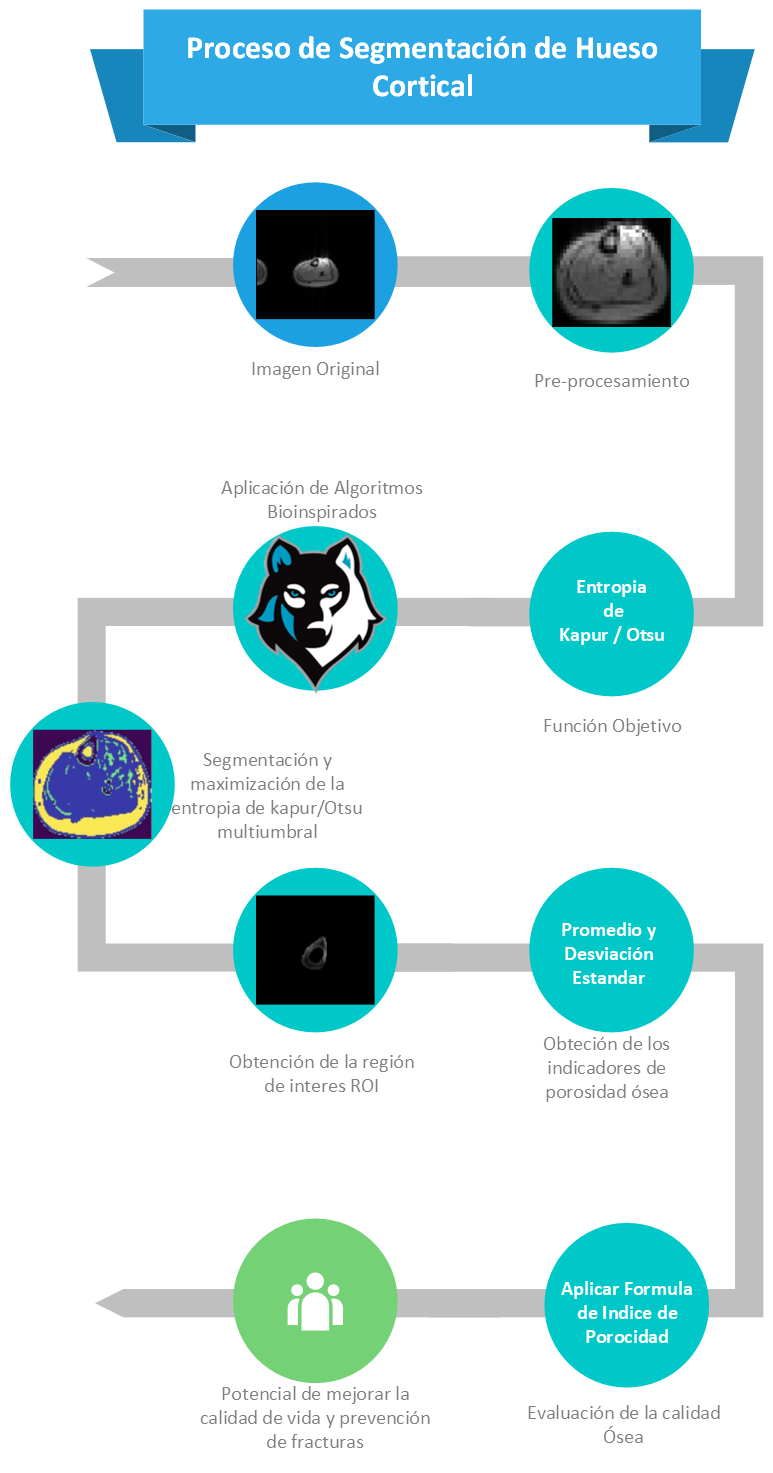
\includegraphics[width=.9\linewidth]{imagenes_hueso/Proceso_Segmentacion_Bioinspirado.png}
	\caption{Representación gráfica del proceso integral, desde la ejecución del algoritmo de segmentación hasta la obtención de los indicadores de salud ósea.}
	\label{fig:z}
\end{figure}

\noindent El objetivo primordial es validar la eficacia y eficiencia de los algoritmos de optimización metaheurísticos en la segmentación de imágenes del hueso cortical.


\section{Trabajos relacionados} \label{sec:rw}

\noindent En el ámbito de la segmentación de imágenes médicas, los algoritmos de optimización metaheurísticos han surgido como herramientas prometedoras, combinando eficacia y versatilidad. Estos algoritmos emulan comportamientos y estrategias observadas en la naturaleza, como la evolución, el comportamiento de enjambres, la caza, entre otros, para resolver problemas complejos en la informática y la optimización ~\cite{Darwish2018}, buscan soluciones óptimas a problemas complejos mediante la exploración y adaptación en el espacio de soluciones. Abualigah et al.\cite{Abualigah2023} realizaron un profundo análisis, destacando la relevancia de estos algoritmos en la segmentación de imágenes multinivel. Al emplear métricas estándar, como la función Fitness, la relación señal-ruido (PSNR) y el índice de similitud estructural (SSIM), se ha evidenciado el potencialidad de estos algoritmos en la mejora de la precisión y calidad en la segmentación de imágenes médicas\cite{Ma2023}.

%\noindent La segmentación de imágenes mediante algoritmos de optimización metaheurísticos ha emergido como un campo de investigación significativo en años recientes. Abualigah et al.~\cite{Abualigah2023} llevaron a cabo un análisis exhaustivo en el que compararon una variedad de algoritmos metaheurísticos para la segmentación de imágenes multinivel. Utilizaron métricas estándar como la función de fitness, la relación señal-ruido (PSNR) y el Índice de Similitud Estructural (SSIM) para evaluar la eficacia de estos algoritmos~\cite{Ma2023}.

\noindent En un enfoque más específico, Bandyopadhyay et al.~\cite{Bandyopadhyay2021} propusieron una versión mejorada del algoritmo de optimización de Harris Hawks (HHO) para la segmentación de imágenes de resonancia magnética cerebral. Esta versión mejorada incorpora conceptos de altruismo e inicialización caótica para potenciar las capacidades de explotación del algoritmo.

\noindent Iswisi et al.~\cite{Iswisi2021} también emplearon el algoritmo HHO, para optimizar la selección de centros en algoritmos de agrupación Fuzzy C-means (FCM). Según sus pruebas en imágenes de resonancia magnética cerebral, el método superó a otros en términos de precisión.


\noindent Xing et al.~\cite{Xing2023} utilizó el agoritmo Artificial Bee Colony (ABC) y la estrategia Elite Levy Spreading (ELS) para la segmentación de imágenes con umbrales multinivel en casos de cáncer de mama y mejorar aún más la calidad óptima de la solución.

\noindent Ryalat et al.~\cite{Ryalat2022} generó diagnóstico de Covid-19 basado en la segmentación de imágenes con umbral multinivel utilizando el algoritmo Harris Hawks optimization (HHO) con la función fitness de umbral Otsu en conjunto de datos públicos sobre imágenes de tórax con correlatos clínicos y genómicos.

\noindent Weizhu et al.~\cite{Weizhu2022} propusieron una versión mejorada del Whale Optimization Algorithm (WOA) llamado LCWOA en la que se introducen el operador Levy y una estrategia caótica de mutación aleatoria para mejorar la capacidad del algoritmo, el cual se aplicó para resolver la selección de umbrales en el problema de segmentación de imágenes de cáncer de piel.

\noindent Peng et al.~\cite{Peng2023} realizaron segmentación de imágenes de umbral multinivel basado en el método Otsu bidimensional y un algoritmo genético mejorado, los resultados indican mejoras en la exactitud y en la eficiencia del algoritmo, perfeccionando también la exactitud del umbral de la imagen y reduciendo la complejidad temporal del algoritmo.

\noindent Sharma et al.~\cite{Sharma2023} ha desarrollado un algoritmo de búsqueda dinámica bioinspirado en el águila calva opuesta (DOBES) mediante el empleo de aprendizaje dinámico de oposición (DOL), un enfoque híbrido de segmentación de imágenes de umbralización multinivel para la segmentación de imágenes de resonancia magnética, la relación señal-ruido (PSNR) y el valor de medida del índice de similitud estructural (SSIM) en comparación con el algoritmo BES para las imágenes de referencia alcanzaron altos valores.

\noindent Xing et al.~\cite{Xing2020} Método de segmentación de imágenes de umbrales múltiples basado en la optimización mejorada del pingüino emperador (EPO). La EPO se utiliza para encontrar los valores de umbral multinivel óptimos para imágenes en color. Luego, se emplean la mutación gaussiana, el vuelo de Levy y el aprendizaje basado en oposición para aumentar la capacidad de búsqueda del algoritmo EPO y equilibrar la explotación y la exploración. El algoritmo IEPO optimiza el método de umbrales múltiples de Kapur para realizar experimentos con imágenes de Berkeley, imágenes de satélite e imágenes de copas de plantas.

\noindent Zhao et al.~\cite{Zhao2023} propone un algoritmo de optimización de colonia de hormigas mejorado llamado LACOR. El algoritmo introduce una estrategia seno coseno (SC), estrategia de búsqueda de alimento disperso (DFS) y estrategia de aprendizaje de reflexión especular (SRL) a la original colonia de hormigas. Un modelo de segmentación multinivel es propuesto utilizando LACOR combinado con la estrategia de medias no locales y la entropía de Kapur aplicada a una imágen patológica de melanoma, para la evaluación se utilizaron las métricas de índice de similitud de características, índice de similitud estructural, relación señal ruido máxima.


\noindent Adicionalmente, se presentan tres estudios recientes que complementan esta revisión:

\begin{itemize}
	\item Malhotra et al.~\cite{Chakraborty2022} ofrecen una revisión exhaustiva sobre el uso de redes neuronales convolucionales profundas en la segmentación de imágenes médicas.
	\item Elyan et al.~\cite{Elyan2022} examinan los avances recientes en visión por computadora y aprendizaje automático aplicados al análisis de imágenes médicas.
	\item An y Liu~\cite{An2020} proponen un algoritmo de segmentación de imágenes médicas basado en una red neuronal convolucional optimizada.
\end{itemize}

\noindent La literatura actual destaca la eficiencia y adaptabilidad de los algoritmos metaheurísticos y de aprendizaje profundo ~\cite{jones2023automated} en la segmentación de imágenes médicas. Sin embargo, múltiples investigaciones se centran en otras áreas del nuestro organismo, dejando de lado las especificidades y retos que presenta la segmentación de imágenes del hueso cortical. Con nuestro estudio, buscamos abordar esta brecha utilizando algoritmos metaheurísticos inspirados en la naturaleza, con la finalidad de proporcionar una solución más precisa y eficaz para la segmentación de imágenes relacionadas con el hueso cortical.

%\noindent Estos trabajos subrayan la eficacia y versatilidad de los algoritmos metaheurísticos y de aprendizaje profundo en la segmentación de imágenes médicas. No obstante, la mayoría se enfoca en imágenes cerebrales y no aborda las particularidades y desafíos de la segmentación de imágenes del hueso cortical. Nuestro trabajo aspira a llenar esta brecha mediante el uso de algoritmos de optimización metaheurísticos bioinspirados, con el objetivo de ofrecer una alternativa más eficiente y precisa para la segmentación de imágenes del hueso cortical.



%(Discute al menos 3 trabajos del contexto de conocimiento en términos de los métodos empíricos utilizados para validar sus efectos, haciendo conclusión de los mismos, relacionada al artefacto propio.)%












\section{Materiales y métodos}

\subsection{Definición del estudio}


\noindent En este trabajo se presenta la segmentación de imágenes del hueso cortical mediante algoritmos de optimización metaheurísticos, considerando este tipo de algoritmos como una aproximación hacia la segmentación automática para el diagnóstico de patologías del hueso cortical. Para determinar los algoritmos con mejor desempeño se aplican los algoritmos de optimización metaheurísticos en un conjunto de datos reales el cual está compuesto por imágenes de resonancia magnéticas del hueso cortical de sujetos de prueba sanos. Los resultados corresponden a la segmentación de imágenes del hueso cortical considerando sus respectivas métricas de segmentación.

\noindent Las variables involucradas corresponden a las métricas de evaluación de la segmentación de las imágenes: función de ajuste, relación máxima de señal-ruido e índice de similitud estructural. Las variables mencionadas son cruciales para evaluar la eficacia de las imágenes segmentadas, ofreciendo una cuantificación precisa de cada algoritmo utilizado. La segmentación precisa del hueso cortical es esencial para un diagnóstico efectivo y una planificación terapéutica.


\noindent Para definir el alcance de la investigación se plantea la siguiente pregunta de investigación: ¿Qué algoritmos de optimización metaheurísticos son apropiados para la segmentación de imágenes del hueso cortical?

\noindent El propósito de este estudio es comparar el desempeño de los algoritmos metaheurísticos en la tarea de segmentación de imágenes de hueso cortical. La investigación es de tipo explicativa, cuantitativa y experimental controlada. Las imágenes fueron recolectadas de pacientes sanos mediante resonancia magnética de bajo campo de 0.55 Teslas. Para realizar la comparación se dispone de 8 algoritmos de optimización metaheurísticos implementados en el entorno de programación Jupyter Notebook con el lenguaje de programación Python. Para comparar el desempeño se utilizaron las métricas de función de ajuste (fitness function) que depende de las dimensiones de la imagen, se considera el mejor valor obtenido por los algoritmos, la relación máxima de señal-ruido (PSNR) que depende de la diferencia entre la imagen segmentada y la imagen original, no posee un rango específico y de igual forma se considera el mayor valor obtenido, y el índice de similitud estructural (SSIM) que posee valores entre 0 y 1, mientras más cercano al 1 mayor será la similitud entre la imagen segmentada. Finalmente, evaluar el numero de iteraciones para encontrar la mejor segmentación.

\noindent Las variables independientes de la investigación corresponden a las imágenes del hueso cortical y los hiperparámetros de los algoritmos de optimización. Por otro lado, las variables dependientes corresponden a  función de ajuste, relación máxima de señal-ruido e índice de similitud estructural.

\noindent Las hipótesis planteadas a partir de la pregunta de investigación corresponden a:
\begin{itemize}
	\item H0. No hay diferencia estadística significativa en el rendimiento de los algoritmos de optimización en función de las métricas PSNR, SSIM y función fitness.
	\item H1. Existe una diferencia estadística significativa en el rendimiento de los algoritmos de optimización en función de las métricas PSNR, SSIM y función Fitness.
\end{itemize}


\subsection{Modelado del problema}

%Problem statement
\noindent La segmentación de imágenes ha sido ampliamente investigada convirtiendo imágenes a color o en escala de grises en imágenes binarias determinando un umbral en la intensidad de píxeles de la imagen~\cite{Sankur2004}. Existen dos tipos de umbralización, una de ellas es binaria y la otra es multinivel. La umbralización binaria consiste en dividir la imagen en dos regiones R1 y R2 a partir de un umbral (th), en este caso se asigna cada pixel $\rho$ a una de las dos regiones como se muestra:.

\begin{equation}
	\begin{gathered}
		\rho \in R_1 \text{ if } 0 \leq \rho < \text{th,} \\
		\rho \in R_2 \text{ if } \text{th} \leq \rho < \text{L-1,}
	\end{gathered}
	\label{eq1}
\end{equation}

\noindent L corresponde al máximo nivel de intensidad.
Por otro lado, la umbralización multinivel consiste en dividir las imágenes en diferentes regiones utilizando más de un umbral como se muesta:

\begin{equation}
	\begin{gathered}
		\rho \in R_1 \text{ if } 0 \leq \rho < \text{th}_1 \\
		\rho \in R_2 \text{ if } \text{th}_1 \leq \rho < \text{th}_2 \\
		\rho \in R_i \text{ if } \text{th}_i \leq \rho < \text{th}_{i+1} \\
		\rho \in R_k \text{ if } \text{th}_{k-1} \leq \rho < \text{L-1}
	\end{gathered}
	\label{eq2}
\end{equation}

\noindent En donde $\{\text{th}_1,\text{th}_2,...,\text{th}_k\}$ corresponde a un vector que representa los diferentes valores de los umbrales.

\noindent Para determinar estos umbrales se utilizan diversos métodos, entre estos destaca la entropía de la imagen, que representa la compacidad y separación entre las clases~\cite{Pun1980}. Uno de estos métodos es la entropía de Kapur, que ha sido ampliamente utilizada para encontrar los valores de umbrales óptimos, maximizando la entropía. Para el caso binario se muestra:

\begin{equation}
	\text{th}^* = \text{max}(F_{kapur}(th))
	\label{eq3}
\end{equation}

\begin{equation}
	F_{kapur}(th) = A_0 + A_1
	\label{eq4}
\end{equation}

\begin{equation}
	\text{A}_0 = - \sum_{i=0}^{th-1} \frac{P_i}{\omega_0} ln\frac{P_i}{\omega_0}, \quad \text{A}_1 = - \sum_{i=th}^{L-1} \frac{P_i}{\omega_0} ln\frac{P_i}{\omega_0}
	\label{eq5}
\end{equation}

\noindent donde $P_i$ es la probabilidad de un nivel de gris $i$, que puede ser representado como:

\begin{equation}
	P_i =\frac{f_i}{\sum_{i=0}^{L-1} f_i}   
	\label{eq6}
\end{equation}

\noindent donde $f_i$ es la frecuencia en el nivel de gris $i$. Por otro lado, se tiene que:

\begin{equation}
	\omega_0 = \sum_{i=0}^{th-1} P_i ,   \omega_1 = \sum_{i=th}^{L-1} P_i
	\label{eq7}
\end{equation}

\noindent En el caso de una umbralización multinivel, se muestra:

\begin{equation}
	\begin{gathered}
		F_{kapur}(th) = A_0 + A_1 + \cdots + A_{k-1} \\
		\text{A}_0 = - \sum_{i=0}^{th_1-1} \frac{P_i}{\omega_0} ln\frac{P_i}{\omega_0}, \quad \omega_0 = \sum_{i=0}^{th_1-1} P_i  \\
		\text{A}_1 = - \sum_{i=th_1}^{th_{2}-1} \frac{P_i}{\omega_1} ln\frac{P_i}{\omega_1}, \quad \omega_1 = \sum_{i=th_1}^{th_{2}-1} P_i \\
		\text{A}_2 = - \sum_{i=th_2}^{th_{3}-1} \frac{P_i}{\omega_2} ln\frac{P_i}{\omega_2}, \quad \omega_2 = \sum_{i=th_2}^{th_{3}-1} P_i \\
		\text{A}_n = - \sum_{i=th_{k-1}}^{L-1} \frac{P_i}{\omega_n} ln\frac{P_i}{\omega_n}, \quad \omega_n = \sum_{i=th_{k-1}}^{L-1} P_i 
	\end{gathered}
	\label{eq8}
\end{equation}

\noindent El símbolo $th$ es un vector que contiene todos los valores de los umbrales.

\noindent Ademas del metodo de la entropia de kapur, se implemento el metodo de Otsu.
\begin{equation}
	\begin{gathered}
		f(\mathbf{t})=\sum_{i=1}^{k+1} w_i (\mu_i - \mu_T)^2 
	\end{gathered}
	\label{eq9}
\end{equation}



donde:
\begin{equation}
	\begin{gathered}
		\mathbf{t} = (t_1, t_2, \dots, t_k) \in \mathbb{Z}^k \text{ es el vector de umbrales} \\
		k = \text{dimensión de la imagen} \\
		\mu_T = \sum_{p=0}^{255} p h(p) \text{ es la media total de la imagen} \\
		h(p) = \text{histograma normalizado el valor de píxel } p \\
		w_i = \sum_{p=l_i}^{u_i} h(p) \text{ es el peso de la clase } i \\
		\mu_i = \frac{1}{w_i} \sum_{p=l_i}^{u_i} p h(p) \text{ es la media de la clase } i \\
		l_i = \begin{cases}
			0 & \text{si } i = 1 \\
			t_{i-2} & \text{en otro caso}
		\end{cases} \\
		u_i = t_i \text{ para } i = 1, 2, \dots, k \\
		u_{k+1} = 256
	\end{gathered}
	\label{eq9}
\end{equation}

\noindent El algoritmo realiza la segmentación de imágenes optimizando la varianza entre clases, basándose en umbrales definidos para los valores de los píxeles. Calcula un histograma de la imagen, y para cada segmento entre umbrales, determina la media ponderada y la contribución a la varianza total. La meta es encontrar los umbrales que maximicen esta varianza total, separando eficazmente la imagen en regiones distintas. Este enfoque es útil para destacar características relevantes dentro de las imágenes, facilitando su análisis y procesamiento.






\subsection{Configuración experimental}

\noindent La experimentación se llevó a cabo en un entorno controlado, aplicando algoritmos metaheurísticos bioinspirados. Estos algoritmos fueron puestos a prueba en imágenes de hueso cortical obtenidas de individuos sanos, Esta decisión se basa en la accesibilidad de los sujetos dentro de la población general, permitiendo así obtener resultados relevantes para un amplio espectro demográfico sin patologías óseas específicas que pudieran sesgar el estudio. El conjunto de imágenes utilizado está compuesto por 20 imágenes de resonancia magnética obtenidas por un resonador de 0.55 Teslas, con diferentes secuencias y tiempos de eco, el conjunto de datos se ilustra en la Figura \ref{fig:imagenes}.
Para mantener la consistencia en los resultados y evitar posibles sesgos en la interpretación, se estableció un tamaño mínimo de imagen de $100\times100$ pixeles como criterio de bloqueo, asegurando así que todas las imágenes estén en un rango adecuado para una segmentación y análisis efectivos.

\begin{figure}
    \centering

    \begin{subfigure}{0.5\textwidth}
        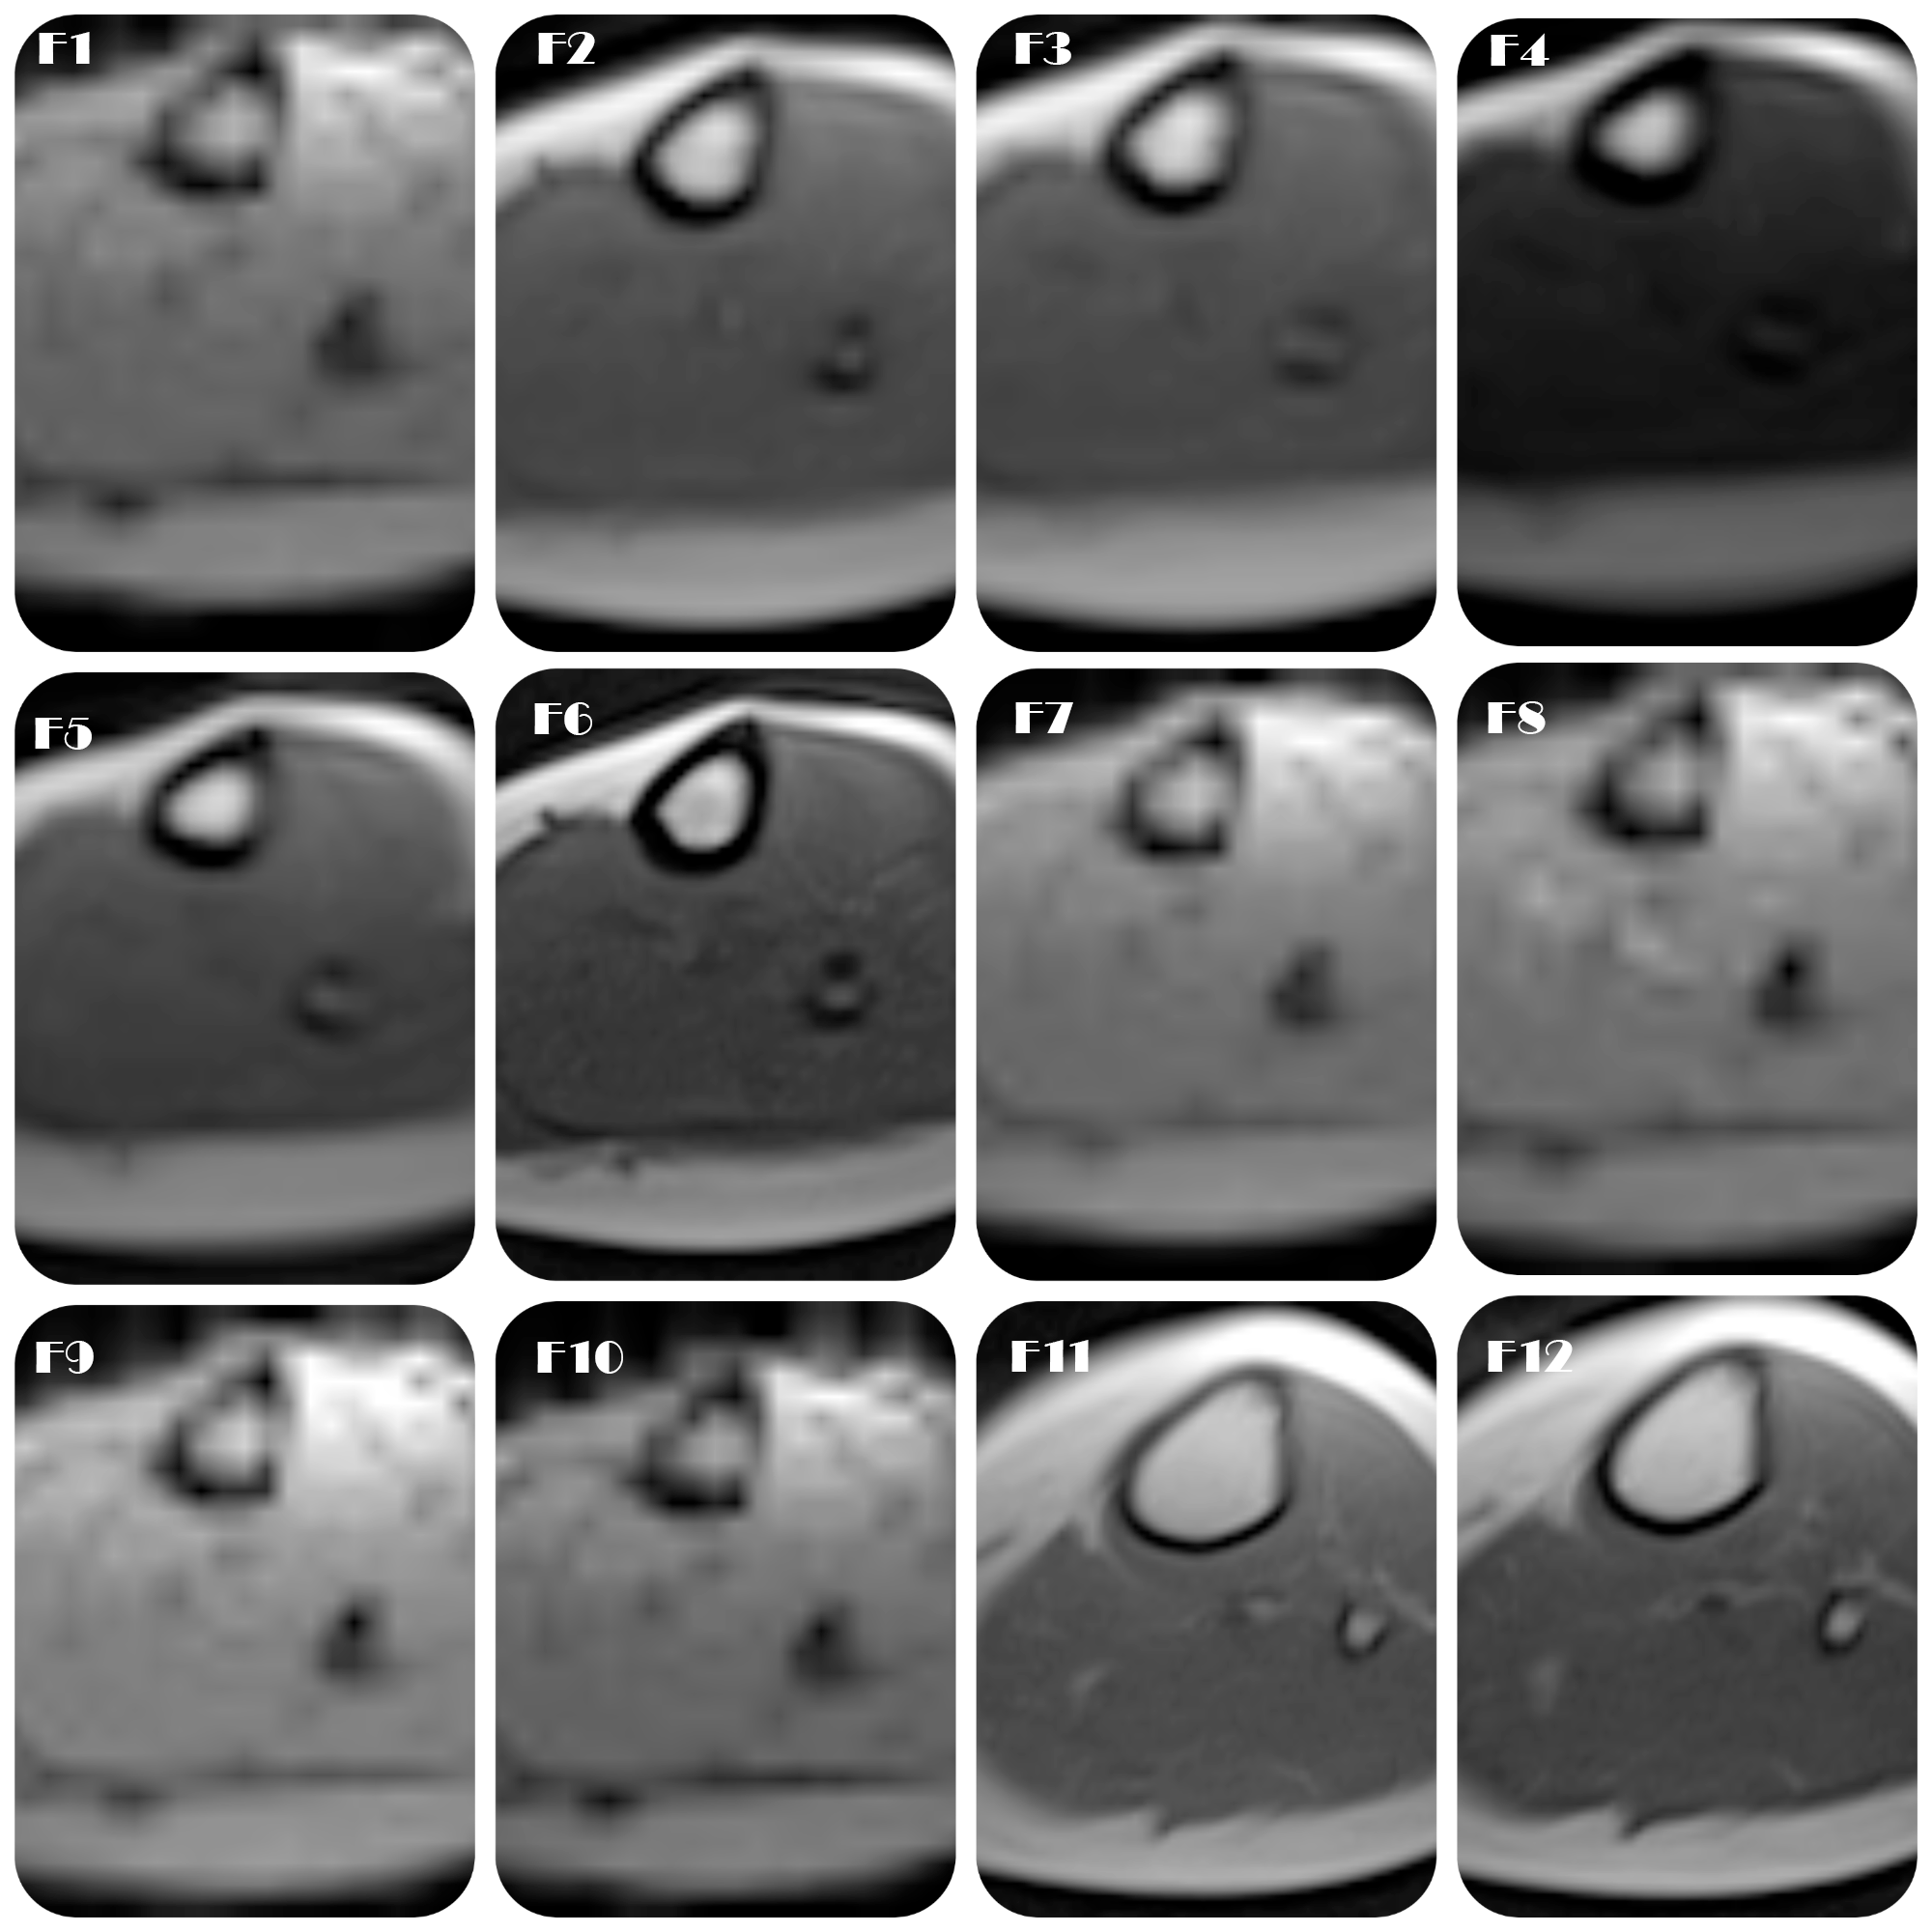
\includegraphics[width=\linewidth]{imagenes_hueso/img_1_12.png}
    \end{subfigure}
    
    \begin{subfigure}{0.5\textwidth}
        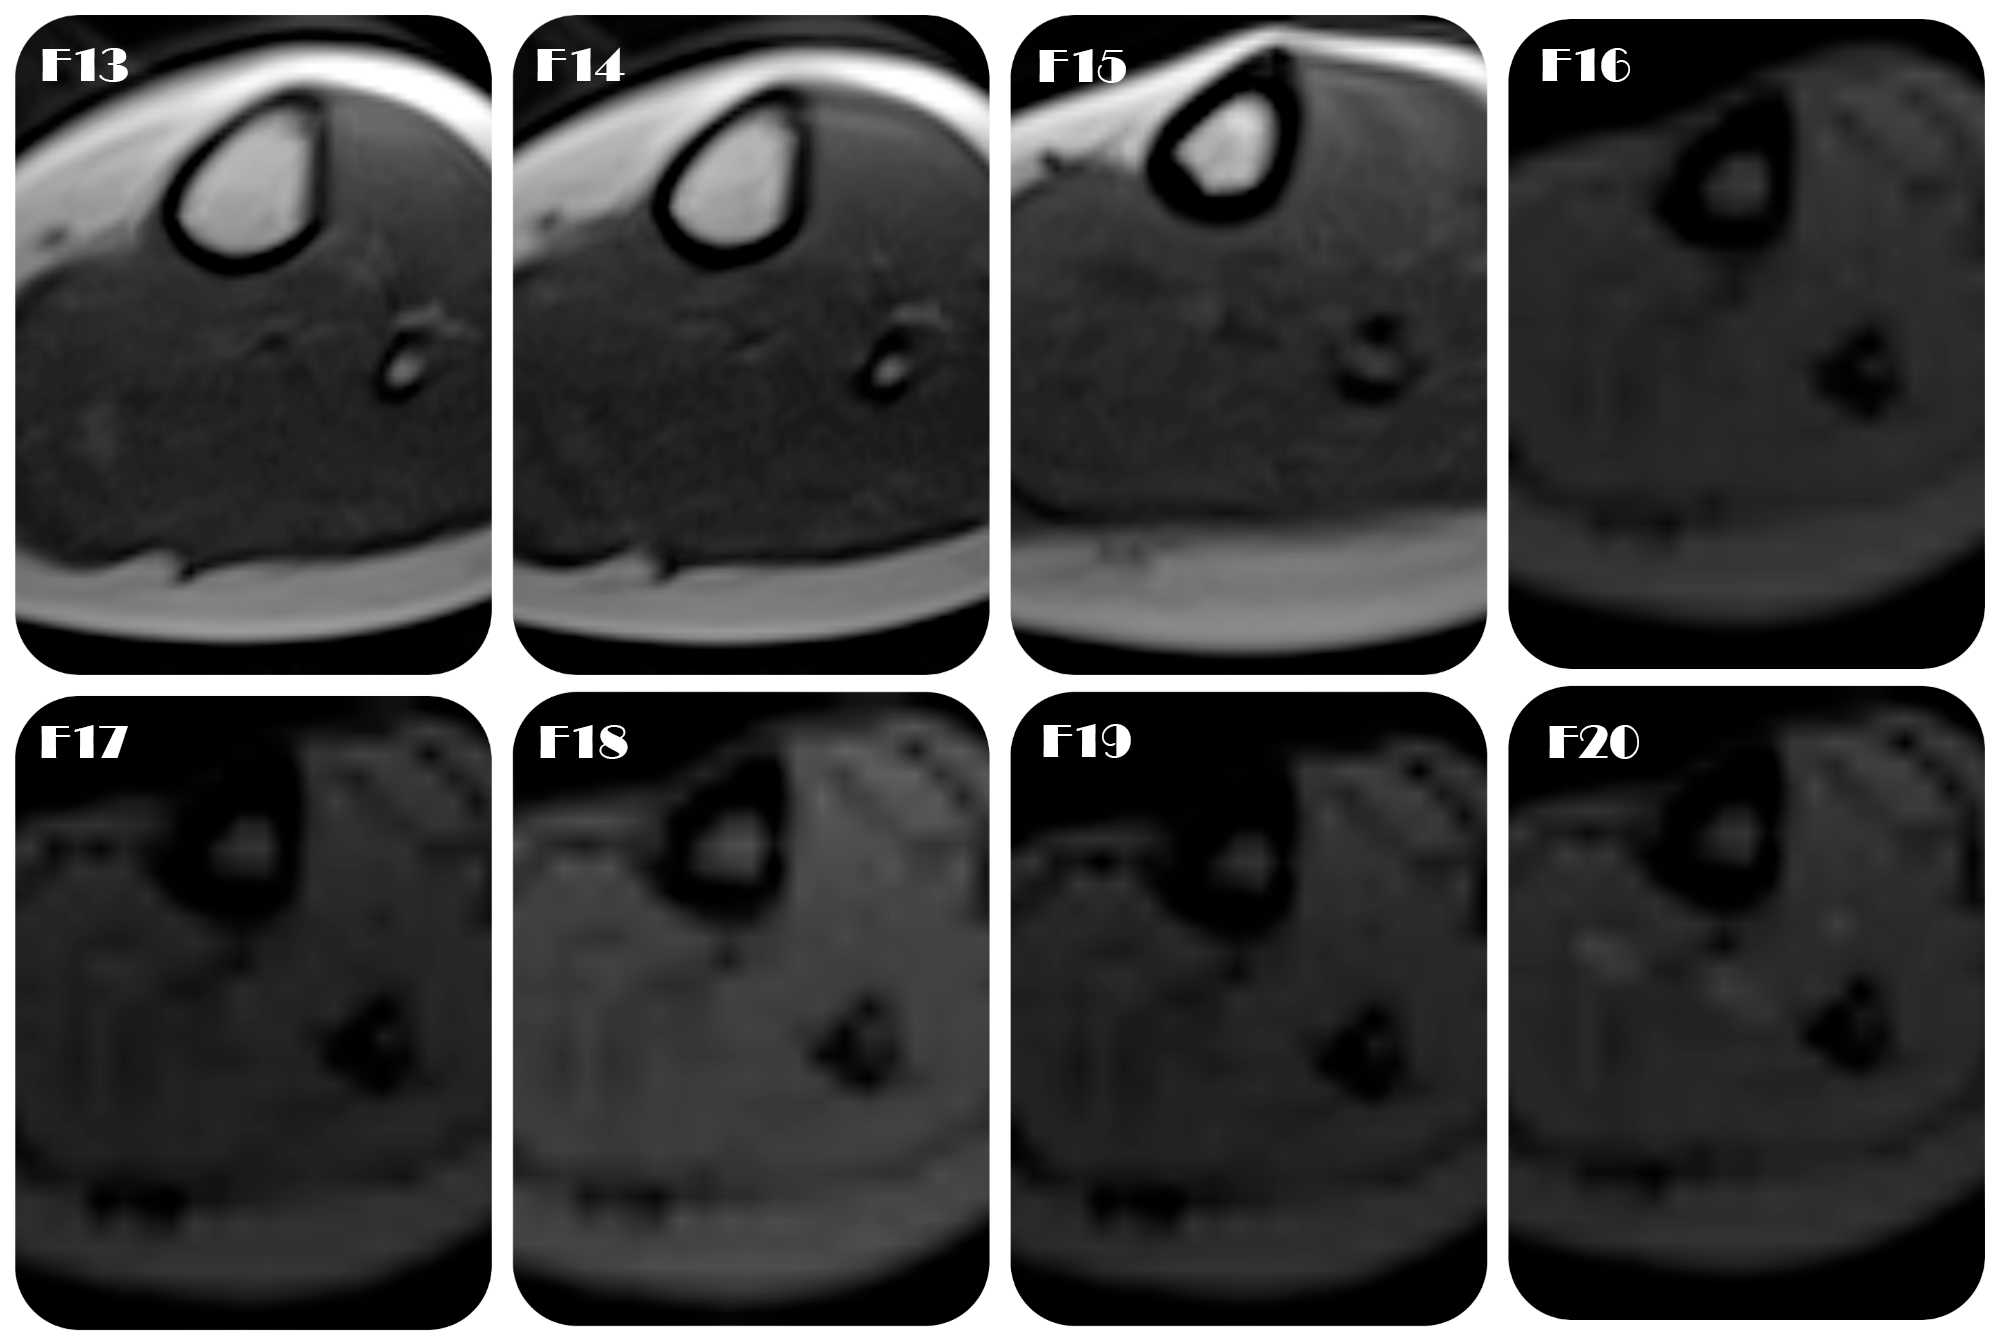
\includegraphics[width=\linewidth]{imagenes_hueso/img_13_20.png}
    \end{subfigure}
    \caption{MRI test images used in the experiments.}
\label{fig:imagenes}    
\end{figure}


\noindent El diseño experimental es multifactorial, enfocándose en tres factores principales: la evaluación de la función fitness, la relación señal-ruido (PSNR) y el Índice de Similitud Estructural (SSIM). Se realizaron ocho tratamientos distintos correspondientes a los algoritmos seleccionados: Reptile Search (RSA)~\cite{Abualigah2022}, Orca Predator (OPA)~\cite{Jiang2022}, Honey Badger Algorithm (HBA)~\cite{Hashim2022}, Bald Eagle Search (BES)~\cite{Alsattar2019}, Gray Wolf Optimization (GWO)~\cite{Mirjalili2014}, Crow Search (CSA)~\cite{Askarzadeh2016}, Harris Hawk Optimization (HHO)~\cite{Heidari2019}  y Tuna Swarm Optimization (TSO)~\cite{Xie2021}. Los parámetros utilizados se tabularon en la Tabla~\ref{tab:algorithms-parameters}, con una población de 30, una iteración fijada en 100 y se realizaron 30 ejecuciones independientes para cada algoritmo.

\begin{table}[!t]
\renewcommand{\arraystretch}{1.3}
\caption{Algoritmos y parámetros}
\label{tab:algorithms-parameters}
\centering
\begin{tabular}{|c|c|}
\hline
\textbf{Algoritmos} & \textbf{parámetros} \\
\hline
BES & 
\begin{tabular}{@{}c@{}}
$c1=c2=2$ \\
$\alpha=2$ \\
$a=10$ \\
$R=1.5$
\end{tabular} \\
\hline
HHO & - \\
\hline
OPA &
\begin{tabular}{@{}c@{}}
$p1,p2=[0,1]$ \\
$a=0.01$
\end{tabular} \\
\hline
CSA &
\begin{tabular}{@{}c@{}}
$fl=2$ \\
$AP=0.1$
\end{tabular} \\
\hline
GWO & $a=2$ (linear decreasing) \\
\hline
HBA &
\begin{tabular}{@{}c@{}}
$\beta=6$ \\
$C=2$
\end{tabular} \\
\hline
RSA &
\begin{tabular}{@{}c@{}}
$\alpha=0.1$ \\
$\beta=0.1$
\end{tabular} \\
\hline
TSO &
\begin{tabular}{@{}c@{}}
$z=0.05$ \\
$a=0.7$
\end{tabular} \\
\hline
\end{tabular}
\end{table}
%Para la implementación de los tratamientos, se utilizó un conjunto de herramientas compuesto por software de procesamiento de imágenes, una plataforma de cómputo con capacidad para ejecutar los algoritmos y realizar cálculos de entropía, PSNR y SSIM de manera eficiente, y scripts en Python para la automatización del análisis. Además, se emplearon bases de datos de imágenes médicas para proporcionar un flujo constante y estandarizado de información al sistema de prueba. Todos los instrumentos y materiales utilizados fueron seleccionados por su probada precisión y fiabilidad, asegurando la integridad y la reproducibilidad de los experimentos.

%Definir variables e hipótesis.
%Algoritmo por si solo es un artefacto
%Algoritmos aplicado al dataaset son tratamientos (justificar los parámetros de las metaheurísticas con trabajos previos)
%Describir el entorno del experimento
%Trabajar con pacientes->Dataset->Algoritmos de optimización->Se comparan utilizando técnicas


%(Define el contexto segun su setting, tipo de problemas, tipo ´de sujetos y generalidad.
%Define variables dependientes e independientes del estudio; las variables a medir son validas anal ´ ´ıtica y emp´ıricamente.
%Define hipotesis nula y alternativa consistentes con la pregunta de investigacion y las mediciones a realizar.)

%La segmentación de imágenes médicas es un área crítica para el diagnóstico y tratamiento de diversas enfermedades. En el contexto de la osteoporosis, el cáncer óseo y otras afecciones relacionadas con el sistema esquelético, la segmentación precisa del hueso cortical es esencial para un diagnóstico efectivo y una planificación terapéutica. Sin embargo, existen limitadas herramientas y técnicas para la evaluación del hueso cortical. Esto no solo compromete la calidad del cuidado médico sino que también puede llevar a tratamientos incorrectos y un aumento en los costos de atención médica. En el ámbito académico y de la investigación, se han aplicado múltiples enfoques para mejorar la segmentación de imágenes médicas, como algoritmos metaheurísticos y redes neuronales convolucionales profundas. No obstante, la mayoría de estos trabajos se enfocan en imágenes cerebrales y carecen de un enfoque específico en la segmentación de imágenes del hueso cortical. Existe, por tanto, una brecha significativa en el estado actual del conocimiento, que hace necesario explorar y desarrollar nuevas metodologías que puedan abordar las particularidades y desafíos de esta área. Ante el panorama actual, tanto social como del conocimiento, el problema que busca abordar este estudio es la falta de algoritmos en la segmentación de imágenes del hueso cortical. Nuestro trabajo aspira a llenar esta brecha mediante el desarrollo y validación de algoritmos de optimización metaheurísticos bioinspirados, con el objetivo de ofrecer una alternativa más eficiente y precisa para la segmentación de este tipo de imágenes médicas.Al definir el problema de esta manera, este estudio espera contribuir tanto al avance de la investigación en técnicas de segmentación de imágenes médicas como a la mejora en la calidad del diagnóstico y tratamiento de enfermedades relacionadas con el hueso cortical.%

%--------------------------------------
\section{Algoritmos metaheurísticos} \label{sec:ds}

\noindent En esta sección, la umbralización multinivel es realizada mediante algoritmos metaheurísticos maximizando la entropía de Kapur ~\ref{eq_Kapur} y Otsu ~\ref{eq_Otsu} como sigue:

\begin{equation}
	\begin{gathered}
		\text{max}(F_{kapur}(th)) \\
		\text{th} \in 0 \leq \text{th}_i \leq 255
	\end{gathered}
	\label{eq_Kapur}
\end{equation}
\noindent En donde $i=[1,2,...,n]$, siendo $n$ la cantidad de umbrales.
\begin{equation}
	\begin{gathered}
		\text{max}(\sigma_B^2(th)) \\
		\text{th} \in 0 \leq \text{th} \leq 255
	\end{gathered}
	\label{eq_Otsu}
\end{equation}

\noindent Aquí, $\sigma_B^2(th)$ representa la varianza entre clases para un umbral $th$, y el objetivo es encontrar el valor de $th$ que maximiza esta varianza, con $th$ variando en el rango de 0 a 255 para imágenes en escala de grises de 8 bits.

\subsection{Bald Eagle Search}

\noindent El algoritmo Bald Eagle Search (BES) propuesto por Alsattar et al.~\cite{Alsattar2019}, es un algoritmo metaheurístico bioinspirado que imita la estrategia de caza o el comportamiento social inteligente de las águilas calvas mientras cazan peces. 

\noindent La etapa de identificación del área se relaciona con el águila calva cuando realiza la búsqueda de la mejor posición $P$ para cazar comida (select space). Esta etapa se representa matemáticamente como:

\begin{equation}
	\begin{gathered}
		P_{new}=P_{best}+{\alpha}r(P_{mean}-P_{i})\\
	\end{gathered}
	\label{eq11}
\end{equation}

\noindent Una vez seleccionada la mejor posición en el espacio, el águila calva realiza diferentes movimientos en espiral para aumentar la velocidad del proceso de búsqueda de comida, a esta etapa se le denomina búsqueda dentro del área (search space) y se representa matemáticamente como:

\begin{equation}
	\begin{gathered}
		P_{new}=P_{i}+y(i)(P_{i}-P_{i+1})+x(i)(P_{i}-P_{mean}) \\
		x(i)= \frac{xr_{i}}{max(\lvert xr \rvert)} ~\ , ~\ y(i)= \frac{yr_{i}}{max(\lvert yr \rvert)} \\
		xr(i)=r(i)\cdot \sin (\theta(i)) ~\ , ~\ yr(i)=r(i)\cdot \cos (\theta(i)) \\
		\theta(i)=a\cdot r\cdot rnd ~\ , ~\ r(i)=\theta(i)+R \cdot rnd 
	\end{gathered}
	\label{eq12}
\end{equation}

\noindent La última etapa del algoritmo BES corresponde a la selección y ataque de la presa, denominada arremetida (swoop). La arremetida consiste en mover todos los mejores puntos hacia el objetivo, matemáticamente esto se expresa como:

\begin{equation}
	\begin{gathered}
		P_{\text{new}} = \text{rnd} \cdot P_{\text{best}} + x1(i)(P_{i}-c1 \cdot P_{\text{mean}}) \\
		+ y1(i)(P_{i}-c2 \cdot P_{\text{best}}) \\
		x1(i) = \frac{xr_{i}}{\max(\lvert xr \rvert)}, \quad y1(i) = \frac{yr_{i}}{\max(\lvert yr \rvert)} \\
		xr(i) = r(i) \cdot \sinh(\theta(i)), \quad yr(i) = r(i) \cdot \cosh(\theta(i))
	\end{gathered}
	\label{eq13}
\end{equation}


\subsection{Harris Hawk Optimization}

\noindent El algoritmo Harris Hawk Optimization (HHO), es un algoritmo bioinspirado propuesto por Heidari et al.~\cite{Heidari2019} basado en el comportamiento de Harris Hawks. El algoritmo fue modelado mediante las fases de exploración y explotación. En la fase de exploración, el Harris Hawk puede detectar y seguir a su presa mediante sus poderosos ojos. En el HHO el Harris Hawk se puede mantener de manera aleatoria en algunas locaciones y esperar a detectar una presa basado en su estrategia. Si se considera una chance igual $q$ para cada estrategia posado basado en la posición de los miembros de su familia, se puede modelar como una condición $q<0.5$, o posado en una posición aleatoria en los árboles como $q\geq 0.5$, como se muestra:
\begin{flalign}
	\begin{gathered}
		X(t+1)= \\
		\begin{cases}
			X_{rnd}(t) - r_1 |X_{rnd}(t) -2 r_2 X(t)| , q \geq 0.5 \\
			X_{rab}(t) - X_m(t) - r3(LB + r_4 (UB-LB)) , q < 0.5   
		\end{cases}
	\end{gathered}
	\label{eq13}
\end{flalign}

La posición promedio se puede calcular mediante:
\begin{equation}
	X_m (t) = \frac{1}{N} \sum_{i=1}^{N} X_i(t) 
	\label{eq14}
\end{equation}

\noindent En la transición de la exploración a la explotación, cuando una presa escapa pierde energía, esta pérdida se modela como:
\begin{equation}
	E = 2 E_0 (1 - \frac{t}{T}) 
	\label{eq15}
\end{equation}

\noindent El parámetro $E$ indica la energía de escape de la presa y $T$ es el máximo número de iteraciones. Por otro lado, $E_0$ es un parámetro aleatorio que oscila entre $(-1,1)$ para cada iteración.

\noindent Por otro lado, la fase de explotación se divide en dos, asedio suave y asedio duro. En el asedio suave se deben cumplir las condiciones de $r \geq 0.5$ y $|E| \geq 0.5$, la presa intenta escapar por algunos saltos aleatorios pero finalmente no puede. Esto se modela como:

\begin{equation}
	\begin{gathered}
		X(t+1) = \Delta X(t) - E |J X_{rabb}(t) -X(t)| \\
		\Delta X(t) = X_{rabb}(t) - X(t)
	\end{gathered}
	\label{eq16}
\end{equation}

\noindent En el asedio duro, se debe cumplir $r \geq 0.5$ y $|E| < 0.5$, la presa está cansada para escapar. En este caso, la posición se actualiza según:

\begin{equation}
	\begin{gathered}
		X(t+1) = X_{rabb}(t) - E |\Delta X(t)| \\
	\end{gathered}
	\label{eq17}
\end{equation}

\subsection{Orca Predator Algorithm}

\noindent El algoritmo Orca Predator (OPA) propuesto por Jiang et al.~\cite{Jiang2022} es un algoritmo metaheurístico bioinspirado en el comportamiento de las Orcas. Las Orcas son seres vivos carnívoros muy inteligentes en la familia de delfines, ellos viven en familias con aproximadamente 30 miembros. Las Orcas se comunican entre ellas con sonidos, en donde coordinan sus movimientos para pastorear peces, llevarlos hacia la superficie y finalmente encerrarlos. El modelo del grupo de Orcas puede nadar en $1-D, 2-D, 3-D$ o en un espacio extradimensional. Esto se define como:

\begin{equation}
	\begin{gathered}
		X = [ x1, x2, ..., xN ] =\begin{bmatrix}
			x1,1 & x1,2 & ... & x1,D  \\
			x2,2 & x2,2 & ... & x2,D  \\
			\vdots & \vdots & \vdots & \vdots \\
			xN,1 & xN,2 & ... & xN,D
		\end{bmatrix}
	\end{gathered}
	\label{eq18}
\end{equation}

\noindent El movimiento de las Orcas pastoreando peces se puede modelar mediante la velocidad de movimiento como sigue:

\begin{equation}
	\begin{gathered}
		v_{chase,1,i}^t = a ( d x_{best}^t - F (b M^t + c x_i^t)) \\
		v_{chase,2,i}^t = e x_{best}^t - x_{i}^t \\
		M = \frac{\sum_{i=1}^{N} x_i^t}{N} \\
		c=1-b \\
		\begin{cases}
			x_{chase,1,i}^t = x_{i}^t + v_{chase,1,i}^t , \text{if} \;rand > q     \\
			x_{chase,2,i}^t = x_{i}^t + v_{chase,2,i}^t  , \text{if} \;rand \leq q 
		\end{cases}
	\end{gathered}
	\label{eq19}
\end{equation}

\noindent El rodeo de presas se realiza mediante la posición de tres Orcas seleccionadas al azar, y luego su posición se puede determinar como:
\begin{equation}
	\begin{gathered}
		x_{chase,3,i}^t =x_{j1,k}^t +u \times (x_{j2,k}^t - x_{j3,k}^t ) \\
		u = 2 \times (\text{rand} - \frac{1}{2}) \times \frac{Max_{iter}-t}{Max_{iter}}
	\end{gathered}
	\label{eq20}
\end{equation}

\noindent El ajuste de posición se determina comparando los mejores valores obtenidos en la función de ajuste, esto se modela como:

\begin{equation}
	\begin{gathered}
		\begin{cases}
			x_{chase,i}^t = x_{chase,i}^t \;\;, \text{if} \; f(x_{chase,i}^t) < f(x_{i}^t ) \\
			x_{chase,t}^t = x_{i}^t  \;\;, \text{if} \;f(x_{chase,i}^t) \geq f(x_{i}^t )    
		\end{cases}
	\end{gathered}
	\label{eq21}
\end{equation}

\noindent En donde $f(x_{chase,i}^t)$ corresponde al valor de la función de ajuste en $x_{chase,i}^t$ y $f(x_{i}^t )$ corresponde al valor de la función de ajuste en $x_{i}^t$.

El ataque de las Orcas se puede modelar como sigue:

\begin{equation}
	\begin{gathered}
		v_{attack,1,i}^t = \frac{(x_{first}^t+x_{second}^t + x_{third}^t + x_{four}^t)}{4-x_{chase,i}^t} \\
		v_{attack,2,i}^t = \frac{(x_{chase,j1}^t+x_{chase,j2}^t + x_{chase,j3}^t}{3-x_{i}^t}  \\
		v_{attack,i}^t = x_{chase,i}^t+ g1 \times v_{attack,1,i}^t + g2 \times v_{attack,2,i}^t
	\end{gathered}
	\label{eq22}
\end{equation}

\subsection{Crow Search Algorithm}

\noindent El algoritmo Crow Search (CSA) propuesto inicialmente por Askarzadeh et al.~\cite{Askarzadeh2016}, es un algoritmo metaheurístico bioinspirado en el comportamiento de los Crows. Los Crows son consideradas las aves más inteligentes, observan a otras aves, observan donde esconden su comida, y las roban cuando no están. De hecho, utilizan su propia experiencia de haber sido ladrones para predecir el comportamiento de un ladrón y pueden determinar el camino más seguro para proteger sus tesoros contra el robo. El primer paso está asociado a la posición y se modela como:

\begin{equation}
	\begin{gathered}
		x^{i,iter} = [x_{1}^{i,iter}, x_{2}^{i,iter},...,x_{d}^{i,iter}]\\
		x^{i,iter+1}=x^{i,iter}+r_{i} \times fl^{i,iter} \times (m^{j,iter}-x^{i,iter})
	\end{gathered}
	\label{eq23}
\end{equation}

\noindent Crow j sabe que crow i lo está siguiendo. Como resultado, para proteger su caché contra el robo, el cuervo j engañará al cuervo i yendo a otra posición del espacio de búsqueda. Esto se modela como:

\begin{equation}
	\begin{gathered}
		x^{i,iter+1}=\\
		\begin{cases}
			x^{i,iter}+r_{i} fl^{i,iter} (m^{j,iter} - x^{i,iter}) \; \; \; r_j \geq AP^{i,iter}                                     \\
			\text{a random position} \; \; \; \; \; \;\; \; \;\; \; \;\;\; \; \;\;\; \; \; \; \;\;\; \; \;\; \; \;  \text{otherwise} 
		\end{cases}
	\end{gathered}
	\label{eq24}
\end{equation}


\subsection{Gray Wolf Optimization}

\noindent El algoritmo Gray Wolf Optimization (GWO) originalmente propuesto por Mirjalili et al.~\cite{Mirjalili2014}, es un algoritmo metaheurístico bioinspirado en el comportamiento de los Gray Wolf, quienes son considerados superdeprepadores, viven en manada y el tamaño grupal suele ir desde los 5 hasta los 12 individuos. Matemáticamente, se considera una jerarquía dentro de la manada, en donde los valores de las soluciones se almacenan en orden, en $\alpha$, $\beta$ y $\delta$, como primero, segundo y tercero respectivamente. El resto de soluciones se almacenan en $\omega$. El algoritmo GWO almacena la caza guiados por $\alpha,\beta$ y $\delta$ mientras que $\omega$ sigue a las otras variables.

\noindent La fase de caza comienza con rodear las presas, esto se modela como:

\begin{equation}
	\begin{gathered}
		\vec{D} = |\vec{C} \times \vec{X_p}(t)-\vec{X}(t)|\\
		\vec{X}(t+1) = \vec{X_p}(t) - \vec{A} \times \vec{D}
	\end{gathered}
	\label{eq25}
\end{equation}

\noindent En donde $\vec{A}$ y $\vec{C}$ son coeficientes del vector y $\vec{X}$ es la posición. La caza es guiada por el alfa, el beta y delta no suelen participar. Matemáticamente, se asume que alfa, beta y delta tienen el mejor conocimiento sobre la posición de las presas. Luego, se almacenan las tres mejores soluciones y se les obliga a los demás agentes a moverse y actualizar sus posiciones acorde a las mejores soluciones.


\begin{equation}
	\begin{gathered}
		\vec{D}_{\alpha} = |\vec{C}_1 \times \vec{X}_{\alpha} -\vec{X}|, \vec{D}_{\beta} = |\vec{C}_1 \times \vec{X}_{\beta} -\vec{X}| \\
		\vec{D}_{\delta} = |\vec{C}_1 \times \vec{X}_{\delta} -\vec{X}|\\
		\vec{X}_1=\vec{D}_{\alpha}-\vec{A}_1 \times (\vec{D}_{\alpha}), \vec{X}_2=\vec{D}_{\beta}-\vec{A}_2 \times (\vec{D}_{\beta})\\
		\vec{X}_3=\vec{D}_{\delta}-\vec{A}_3 \times (\vec{D}_{\delta}) \\
		\vec{X}(t+1) = \frac{\vec{X}_1+\vec{X}_2+\vec{X}_3}{3}
	\end{gathered}
	\label{eq26}
\end{equation}


\subsection{Honey Badger Algorithm}

\noindent El algoritmo Honey Badger Algorithm (HBA) originalmente propuesto por Hashim et al.~\cite{Hashim2022}, es un algoritmo metaheurístico bioinspirado basado en el comportamiento de los Honey Badger. El Honey Badger realiza seguimientos al pájaro guía de la miel, también puede oler y excavar aquellos lugares en donde se haya miel. El pájaro guía de la miel no tiene la capacidad de excavar para encontrar la miel, por otro lado el Honey Badger si puede excavar, es común que tanto el pájaro de la miel como el Honey Bagder compartan la recompensa. La población de soluciones candidatas se modela como:

\begin{equation}
	\begin{gathered}
		Population \;of\; candidates\; solutions=\\\begin{bmatrix}
			x1,1 & x1,2 & ... & x1,D  \\
			x2,2 & x2,2 & ... & x2,D  \\
			\vdots & \vdots & \vdots & \vdots \\
			xn,1 & xn,2 & ... & xn,D
		\end{bmatrix}
	\end{gathered}
	\label{eq27}
\end{equation}

\noindent La intensidad está relacionada con el poder de concentración de la presa y la distancia entre este y el $ith$ Honey Badger. La intensidad del olor de la presa es representada mediante $I_i$, si el olor es alto el movimiento será rápido y viceversa. Esto se define como:

\begin{equation}
	\begin{gathered}
		I_1 = r_2 \times \frac{S}{4 \pi d_i^2}\\
		S = (x_i -x_{i+1})^2\\
		d_i = x_{prey} - x_i
	\end{gathered}
	\label{eq28}
\end{equation}

\noindent $S$ representa el poder de concentración, $d_i$ denota la distancia entre la presa y el $ith$ Honey Badger. Por otro lado, el factor de densidad $\alpha$ controla la aleatorización del tiempo variante para asegurar la transición de la exploración a la explotación, como se muestra:

\begin{equation}
	\begin{gathered}
		\alpha = C \times exp (\frac{-t}{t_{max}})\\
	\end{gathered}
	\label{eq29}
\end{equation}

\noindent En la fase de excavación el Honey Bagder realiza un movimiento cardioide, como sigue:

\begin{equation}
	\begin{gathered}
		x_{new}=x_{prey}+F \times \beta \times I x_{prey} + \\
		F \times r_3 \times \alpha \times d_i  \times |cos(2\pi r_4) \times [1-cos(2\pi r_5)]|
	\end{gathered}
	\label{eq30}
\end{equation}

\noindent $x_{prey}$ corresponde a la posición de la presa, $r_3$, $r_4$ y $r_5$ son números aleatorios entre 0 y 1. $F$ actúa como una flag que altera la dirección de búsqueda, como sigue:

\begin{equation}
	\begin{gathered}
		F=
		\begin{cases}
			1, \; \; if \; r_6 \leq 0.5 \\
			-1 \; \; else               
		\end{cases}
	\end{gathered}
	\label{eq31}
\end{equation}    

\noindent $r_6$ es un número aleatorio entre 0 y 1.Finalmente, la posición es actualizada por el pájaro guía de la miel, que se puede simular como:

\begin{equation}
	\begin{gathered}
		x_{new}=x_{prey}+F\times r_7\times \alpha \times d_i
	\end{gathered}
	\label{eq32}
\end{equation}

\noindent $r_7$ es un número aleatorio entre 0 y 1.

\subsection{Reptile Search Algorithm}

\noindent El algoritmo Reptile Search (RSA) originalmente propuesto por Abualigah et al.~\cite{Abualigah2022} está basado en el comportamiento de los cocodrilos durante la caza. 
\noindent La ecuación 1 es generada de manera estocástica, y la mejor solución es considerada la más cercana al óptimo en cada iteración.
\begin{equation}
	\begin{gathered}
		X= \begin{bmatrix}
			x1,1 & x1,2 & ... & x1,n  \\
			x2,2 & x2,2 & ... & x2,n  \\
			\vdots & \vdots & \vdots & \vdots \\
			xN,1 & xN,2 & ... & xN,n
		\end{bmatrix}
	\end{gathered}
	\label{eq33}
\end{equation}

\noindent La fase de exploración está definida por:

\begin{equation}
	\begin{gathered}
		x_{(i,j)}(t+1)=\\
		\begin{cases}
			Best_j (t) - \eta_{(i,j)}\times \beta-R_{(i,j)}(t)\times rand, \; \; \; t \leq \frac{T}{4}               \\
			Best_j (t) \times x_{(r_1,j)} \times ES(t) \times rand, \; \; t \leq 2\frac{T}{4} and t \geq \frac{T}{4} \\
		\end{cases}
	\end{gathered}
	\label{eq34}
\end{equation}   

\begin{equation}
	\begin{gathered}
		\eta_{(i,j)}=Best_j(t)\times P_{(i,j)}
	\end{gathered}
	\label{eq35}
\end{equation}

\begin{equation}
	\begin{gathered}
		R_{(i,j)}=\frac{Best_j(t) - x_{(r_2,j)}}{Best_j(t) +\epsilon}
	\end{gathered}
	\label{eq36}
\end{equation}

\begin{equation}
	\begin{gathered}
		ES(t)=2 \times r_3 \times (1 - \frac{1}{T})
	\end{gathered}
	\label{eq37}
\end{equation}

\begin{equation}
	\begin{gathered}
		P_{(i,j)}=\alpha + \frac{x_{(i,j) - M(x_i)}}{Best_j(t) \times (UB_{(j)}-LB_{(j)})+\epsilon} 
	\end{gathered}
	\label{eq38}
\end{equation}

\begin{equation}
	\begin{gathered}
		M_{(x_i)} = \frac{1}{n} \sum_{j=1}^{n} x_{(i,j)}
	\end{gathered}
	\label{eq39}
\end{equation}

\subsection{Tuna Swarm Optimization}

\noindent El algoritmo propuesto por Xie et al.~\cite{Xie2021}


\noindent En esta sección, la umbralización multinivel es realizada mediante algoritmos metaheurísticos maximizando la entropía de Kapur como sigue:

\begin{equation}
	\begin{gathered}
		\text{max}(F_{kapur}(th)) \\
		\text{th} \in 0 \leq \text{th}_i \leq 255
	\end{gathered}
	\label{eq10}
\end{equation}

\noindent En donde $i=[1,2,...,n]$, siendo $n$ la cantidad de umbrales.

\subsection{Bald Eagle Search}

\noindent El algoritmo Bald Eagle Search (BES) propuesto por Alsattar et al.~\cite{Alsattar2019}, es un algoritmo metaheurístico bioinspirado que imita la estrategia de caza o el comportamiento social inteligente de las águilas calvas mientras cazan peces. 

\noindent La etapa de identificación del área se relaciona con el águila calva cuando realiza la búsqueda de la mejor posición $P$ para cazar comida (select space). Esta etapa se representa matemáticamente como:

\begin{equation}
	\begin{gathered}
		P_{new}=P_{best}+{\alpha}r(P_{mean}-P_{i})\\
	\end{gathered}
	\label{eq11}
\end{equation}

\noindent Una vez seleccionada la mejor posición en el espacio, el águila calva realiza diferentes movimientos en espiral para aumentar la velocidad del proceso de búsqueda de comida, a esta etapa se le denomina búsqueda dentro del área (search space) y se representa matemáticamente como:

\begin{equation}
	\begin{gathered}
		P_{new}=P_{i}+y(i)(P_{i}-P_{i+1})+x(i)(P_{i}-P_{mean}) \\
		x(i)= \frac{xr_{i}}{max(\lvert xr \rvert)} ~\ , ~\ y(i)= \frac{yr_{i}}{max(\lvert yr \rvert)} \\
		xr(i)=r(i)\cdot \sin (\theta(i)) ~\ , ~\ yr(i)=r(i)\cdot \cos (\theta(i)) \\
		\theta(i)=a\cdot r\cdot rnd ~\ , ~\ r(i)=\theta(i)+R \cdot rnd 
	\end{gathered}
	\label{eq12}
\end{equation}

\noindent La última etapa del algoritmo BES corresponde a la selección y ataque de la presa, denominada arremetida (swoop). La arremetida consiste en mover todos los mejores puntos hacia el objetivo, matemáticamente esto se expresa como:

\begin{equation}
	\begin{gathered}
		P_{\text{new}} = \text{rnd} \cdot P_{\text{best}} + x1(i)(P_{i}-c1 \cdot P_{\text{mean}}) \\
		+ y1(i)(P_{i}-c2 \cdot P_{\text{best}}) \\
		x1(i) = \frac{xr_{i}}{\max(\lvert xr \rvert)}, \quad y1(i) = \frac{yr_{i}}{\max(\lvert yr \rvert)} \\
		xr(i) = r(i) \cdot \sinh(\theta(i)), \quad yr(i) = r(i) \cdot \cosh(\theta(i))
	\end{gathered}
	\label{eq13}
\end{equation}


\subsection{Harris Hawk Optimization}

\noindent El algoritmo Harris Hawk Optimization (HHO), es un algoritmo bioinspirado propuesto por Heidari et al.~\cite{Heidari2019} basado en el comportamiento de Harris Hawks. El algoritmo fue modelado mediante las fases de exploración y explotación. En la fase de exploración, el Harris Hawk puede detectar y seguir a su presa mediante sus poderosos ojos. En el HHO el Harris Hawk se puede mantener de manera aleatoria en algunas locaciones y esperar a detectar una presa basado en su estrategia. Si se considera una chance igual $q$ para cada estrategia posado basado en la posición de los miembros de su familia, se puede modelar como una condición $q<0.5$, o posado en una posición aleatoria en los árboles como $q\geq 0.5$, como se muestra:
\begin{flalign}
	\begin{gathered}
		X(t+1)= \\
		\begin{cases}
			X_{rnd}(t) - r_1 |X_{rnd}(t) -2 r_2 X(t)| , q \geq 0.5 \\
			X_{rab}(t) - X_m(t) - r3(LB + r_4 (UB-LB)) , q < 0.5   
		\end{cases}
	\end{gathered}
	\label{eq13}
\end{flalign}

\noindent La posición promedio se puede calcular mediante:
\begin{equation}
	X_m (t) = \frac{1}{N} \sum_{i=1}^{N} X_i(t) 
	\label{eq14}
\end{equation}

\noindent En la transición de la exploración a la explotación, cuando una presa escapa pierde energía, esta pérdida se modela como:
\begin{equation}
	E = 2 E_0 (1 - \frac{t}{T}) 
	\label{eq15}
\end{equation}

\noindent El parámetro $E$ indica la energía de escape de la presa y $T$ es el máximo número de iteraciones. Por otro lado, $E_0$ es un parámetro aleatorio que oscila entre $(-1,1)$ para cada iteración.

\noindent Por otro lado, la fase de explotación se divide en dos, asedio suave y asedio duro. En el asedio suave se deben cumplir las condiciones de $r \geq 0.5$ y $|E| \geq 0.5$, la presa intenta escapar por algunos saltos aleatorios pero finalmente no puede. Esto se modela como:

\begin{equation}
	\begin{gathered}
		X(t+1) = \Delta X(t) - E |J X_{rabb}(t) -X(t)| \\
		\Delta X(t) = X_{rabb}(t) - X(t)
	\end{gathered}
	\label{eq16}
\end{equation}

\noindent En el asedio duro, se debe cumplir $r \geq 0.5$ y $|E| < 0.5$, la presa está cansada para escapar. En este caso, la posición se actualiza según:

\begin{equation}
	\begin{gathered}
		X(t+1) = X_{rabb}(t) - E |\Delta X(t)| \\
	\end{gathered}
	\label{eq17}
\end{equation}

\subsection{Orca Predator Algorithm}

\noindent El algoritmo Orca Predator (OPA) propuesto por Jiang et al.~\cite{Jiang2022} es un algoritmo metaheurístico bioinspirado en el comportamiento de las Orcas. Las Orcas son seres vivos carnívoros muy inteligentes en la familia de delfines, ellos viven en familias con aproximadamente 30 miembros. Las Orcas se comunican entre ellas con sonidos, en donde coordinan sus movimientos para pastorear peces, llevarlos hacia la superficie y finalmente encerrarlos. El modelo del grupo de Orcas puede nadar en $1-D, 2-D, 3-D$ o en un espacio extradimensional. Esto se define como:

\begin{equation}
	\begin{gathered}
		X = [ x1, x2, ..., xN ] =\begin{bmatrix}
			x1,1 & x1,2 & ... & x1,D  \\
			x2,2 & x2,2 & ... & x2,D  \\
			\vdots & \vdots & \vdots & \vdots \\
			xN,1 & xN,2 & ... & xN,D
		\end{bmatrix}
	\end{gathered}
	\label{eq18}
\end{equation}

\noindent El movimiento de las Orcas pastoreando peces se puede modelar mediante la velocidad de movimiento como sigue:

\begin{equation}
	\begin{gathered}
		v_{chase,1,i}^t = a ( d x_{best}^t - F (b M^t + c x_i^t)) \\
		v_{chase,2,i}^t = e x_{best}^t - x_{i}^t \\
		M = \frac{\sum_{i=1}^{N} x_i^t}{N} \\
		c=1-b \\
		\begin{cases}
			x_{chase,1,i}^t = x_{i}^t + v_{chase,1,i}^t , \text{if} \;rand > q     \\
			x_{chase,2,i}^t = x_{i}^t + v_{chase,2,i}^t  , \text{if} \;rand \leq q 
		\end{cases}
	\end{gathered}
	\label{eq19}
\end{equation}

\noindent El rodeo de presas se realiza mediante la posición de tres Orcas seleccionadas al azar, y luego su posición se puede determinar como:
\begin{equation}
	\begin{gathered}
		x_{chase,3,i}^t =x_{j1,k}^t +u \times (x_{j2,k}^t - x_{j3,k}^t ) \\
		u = 2 \times (\text{rand} - \frac{1}{2}) \times \frac{Max_{iter}-t}{Max_{iter}}
	\end{gathered}
	\label{eq20}
\end{equation}

\noindent El ajuste de posición se determina comparando los mejores valores obtenidos en la función de ajuste, esto se modela como:

\begin{equation}
	\begin{gathered}
		\begin{cases}
			x_{chase,i}^t = x_{chase,i}^t \;\;, \text{if} \; f(x_{chase,i}^t) < f(x_{i}^t ) \\
			x_{chase,t}^t = x_{i}^t  \;\;, \text{if} \;f(x_{chase,i}^t) \geq f(x_{i}^t )    
		\end{cases}
	\end{gathered}
	\label{eq21}
\end{equation}

\noindent En donde $f(x_{chase,i}^t)$ corresponde al valor de la función de ajuste en $x_{chase,i}^t$ y $f(x_{i}^t )$ corresponde al valor de la función de ajuste en $x_{i}^t$.

El ataque de las Orcas se puede modelar como sigue:

\begin{equation}
	\begin{gathered}
		v_{attack,1,i}^t = \frac{(x_{first}^t+x_{second}^t + x_{third}^t + x_{four}^t)}{4-x_{chase,i}^t} \\
		v_{attack,2,i}^t = \frac{(x_{chase,j1}^t+x_{chase,j2}^t + x_{chase,j3}^t}{3-x_{i}^t}  \\
		v_{attack,i}^t = x_{chase,i}^t+ g1 \times v_{attack,1,i}^t + g2 \times v_{attack,2,i}^t
	\end{gathered}
	\label{eq22}
\end{equation}

\subsection{Crow Search Algorithm}

\noindent El algoritmo Crow Search (CSA) propuesto inicialmente por Askarzadeh et al.~\cite{Askarzadeh2016}, es un algoritmo metaheurístico bioinspirado en el comportamiento de los Crows. Los Crows son consideradas las aves más inteligentes, observan a otras aves, observan donde esconden su comida, y las roban cuando no están. De hecho, utilizan su propia experiencia de haber sido ladrones para predecir el comportamiento de un ladrón y pueden determinar el camino más seguro para proteger sus tesoros contra el robo. El primer paso está asociado a la posición y se modela como:

\begin{equation}
	\begin{gathered}
		x^{i,iter} = [x_{1}^{i,iter}, x_{2}^{i,iter},...,x_{d}^{i,iter}]\\
		x^{i,iter+1}=x^{i,iter}+r_{i} \times fl^{i,iter} \times (m^{j,iter}-x^{i,iter})
	\end{gathered}
	\label{eq23}
\end{equation}

\noindent Crow j sabe que crow i lo está siguiendo. Como resultado, para proteger su caché contra el robo, el cuervo j engañará al cuervo i yendo a otra posición del espacio de búsqueda. Esto se modela como:

\begin{equation}
	\begin{gathered}
		x^{i,iter+1}=\\
		\begin{cases}
			x^{i,iter}+r_{i} fl^{i,iter} (m^{j,iter} - x^{i,iter}) \; \; \; r_j \geq AP^{i,iter}                                     \\
			\text{a random position} \; \; \; \; \; \;\; \; \;\; \; \;\;\; \; \;\;\; \; \; \; \;\;\; \; \;\; \; \;  \text{otherwise} 
		\end{cases}
	\end{gathered}
	\label{eq24}
\end{equation}


\subsection{Gray Wolf Optimization}

\noindent El algoritmo Gray Wolf Optimization (GWO) originalmente propuesto por Mirjalili et al.~\cite{Mirjalili2014}, es un algoritmo metaheurístico bioinspirado en el comportamiento de los Gray Wolf, quienes son considerados superdeprepadores, viven en manada y el tamaño grupal suele ir desde los 5 hasta los 12 individuos. Matemáticamente, se considera una jerarquía dentro de la manada, en donde los valores de las soluciones se almacenan en orden, en $\alpha$, $\beta$ y $\delta$, como primero, segundo y tercero respectivamente. El resto de soluciones se almacenan en $\omega$. El algoritmo GWO almacena la caza guiados por $\alpha,\beta$ y $\delta$ mientras que $\omega$ sigue a las otras variables.

\noindent La fase de caza comienza con rodear las presas, esto se modela como:

\begin{equation}
	\begin{gathered}
		\vec{D} = |\vec{C} \times \vec{X_p}(t)-\vec{X}(t)|\\
		\vec{X}(t+1) = \vec{X_p}(t) - \vec{A} \times \vec{D}
	\end{gathered}
	\label{eq25}
\end{equation}

\noindent En donde $\vec{A}$ y $\vec{C}$ son coeficientes del vector y $\vec{X}$ es la posición. La caza es guiada por el alfa, el beta y delta no suelen participar. Matemáticamente, se asume que alfa, beta y delta tienen el mejor conocimiento sobre la posición de las presas. Luego, se almacenan las tres mejores soluciones y se les obliga a los demás agentes a moverse y actualizar sus posiciones acorde a las mejores soluciones.


\begin{equation}
	\begin{gathered}
		\vec{D}_{\alpha} = |\vec{C}_1 \times \vec{X}_{\alpha} -\vec{X}|, \vec{D}_{\beta} = |\vec{C}_1 \times \vec{X}_{\beta} -\vec{X}| \\
		\vec{D}_{\delta} = |\vec{C}_1 \times \vec{X}_{\delta} -\vec{X}|\\
		\vec{X}_1=\vec{D}_{\alpha}-\vec{A}_1 \times (\vec{D}_{\alpha}), \vec{X}_2=\vec{D}_{\beta}-\vec{A}_2 \times (\vec{D}_{\beta})\\
		\vec{X}_3=\vec{D}_{\delta}-\vec{A}_3 \times (\vec{D}_{\delta}) \\
		\vec{X}(t+1) = \frac{\vec{X}_1+\vec{X}_2+\vec{X}_3}{3}
	\end{gathered}
	\label{eq26}
\end{equation}


\subsection{Honey Badger Algorithm}

\noindent El algoritmo Honey Badger Algorithm (HBA) originalmente propuesto por Hashim et al.~\cite{Hashim2022}, es un algoritmo metaheurístico bioinspirado basado en el comportamiento de los Honey Badger. El Honey Badger realiza seguimientos al pájaro guía de la miel, también puede oler y excavar aquellos lugares en donde se haya miel. El pájaro guía de la miel no tiene la capacidad de excavar para encontrar la miel, por otro lado el Honey Badger si puede excavar, es común que tanto el pájaro de la miel como el Honey Bagder compartan la recompensa. La población de soluciones candidatas se modela como:

\begin{equation}
	\begin{gathered}
		Population \;of\; candidates\; solutions=\\\begin{bmatrix}
			x1,1 & x1,2 & ... & x1,D  \\
			x2,2 & x2,2 & ... & x2,D  \\
			\vdots & \vdots & \vdots & \vdots \\
			xn,1 & xn,2 & ... & xn,D
		\end{bmatrix}
	\end{gathered}
	\label{eq27}
\end{equation}

\noindent La intensidad está relacionada con el poder de concentración de la presa y la distancia entre este y el $ith$ Honey Badger. La intensidad del olor de la presa es representada mediante $I_i$, si el olor es alto el movimiento será rápido y viceversa. Esto se define como:

\begin{equation}
	\begin{gathered}
		I_1 = r_2 \times \frac{S}{4 \pi d_i^2}\\
		S = (x_i -x_{i+1})^2\\
		d_i = x_{prey} - x_i
	\end{gathered}
	\label{eq28}
\end{equation}

\noindent $S$ representa el poder de concentración, $d_i$ denota la distancia entre la presa y el $ith$ Honey Badger. Por otro lado, el factor de densidad $\alpha$ controla la aleatorización del tiempo variante para asegurar la transición de la exploración a la explotación, como se muestra:

\begin{equation}
	\begin{gathered}
		\alpha = C \times exp (\frac{-t}{t_{max}})\\
	\end{gathered}
	\label{eq29}
\end{equation}

\noindent En la fase de excavación el Honey Bagder realiza un movimiento cardioide, como sigue:

\begin{equation}
	\begin{gathered}
		x_{new}=x_{prey}+F \times \beta \times I x_{prey} + \\
		F \times r_3 \times \alpha \times d_i  \times |cos(2\pi r_4) \times [1-cos(2\pi r_5)]|
	\end{gathered}
	\label{eq30}
\end{equation}

\noindent $x_{prey}$ corresponde a la posición de la presa, $r_3$, $r_4$ y $r_5$ son números aleatorios entre 0 y 1. $F$ actúa como una flag que altera la dirección de búsqueda, como sigue:

\begin{equation}
	\begin{gathered}
		F=
		\begin{cases}
			1, \; \; if \; r_6 \leq 0.5 \\
			-1 \; \; else               
		\end{cases}
	\end{gathered}
	\label{eq31}
\end{equation}    

\noindent $r_6$ es un número aleatorio entre 0 y 1.Finalmente, la posición es actualizada por el pájaro guía de la miel, que se puede simular como:

\begin{equation}
	\begin{gathered}
		x_{new}=x_{prey}+F\times r_7\times \alpha \times d_i
	\end{gathered}
	\label{eq32}
\end{equation}

\noindent $r_7$ es un número aleatorio entre 0 y 1.

\subsection{Reptile Search Algorithm}

\noindent El algoritmo Reptile Search (RSA) originalmente propuesto por Abualigah et al.~\cite{Abualigah2022} está basado en el comportamiento de los cocodrilos durante la caza. 
\noindent La ecuación 1 es generada de manera estocástica, y la mejor solución es considerada la más cercana al óptimo en cada iteración.
\begin{equation}
	\begin{gathered}
		X= \begin{bmatrix}
			x1,1 & x1,2 & ... & x1,n  \\
			x2,2 & x2,2 & ... & x2,n  \\
			\vdots & \vdots & \vdots & \vdots \\
			xN,1 & xN,2 & ... & xN,n
		\end{bmatrix}
	\end{gathered}
	\label{eq33}
\end{equation}

\noindent La fase de exploración está definida por:

\begin{equation}
	\small
	\begin{gathered}
		x_{(i,j)}(t+1)=\\
		\begin{cases}
			Best_j (t) - \eta_{(i,j)}\times \beta-R_{(i,j)}(t)\times rand, \; \; \; t \leq \frac{T}{4}               \\
			Best_j (t) \times x_{(r_1,j)} \times ES(t) \times rand, \; \; t \leq 2\frac{T}{4} and t \geq \frac{T}{4} \\
		\end{cases}
	\end{gathered}
	\label{eq34}
\end{equation}   

\begin{equation}
	\begin{gathered}
		\eta_{(i,j)}=Best_j(t)\times P_{(i,j)}
	\end{gathered}
	\label{eq35}
\end{equation}

\begin{equation}
	\begin{gathered}
		R_{(i,j)}=\frac{Best_j(t) - x_{(r_2,j)}}{Best_j(t) +\epsilon}
	\end{gathered}
	\label{eq36}
\end{equation}

\begin{equation}
	\begin{gathered}
		ES(t)=2 \times r_3 \times (1 - \frac{1}{T})
	\end{gathered}
	\label{eq37}
\end{equation}

\begin{equation}
	\begin{gathered}
		P_{(i,j)}=\alpha + \frac{x_{(i,j) - M(x_i)}}{Best_j(t) \times (UB_{(j)}-LB_{(j)})+\epsilon} 
	\end{gathered}
	\label{eq38}
\end{equation}

\begin{equation}
	\begin{gathered}
		M_{(x_i)} = \frac{1}{n} \sum_{j=1}^{n} x_{(i,j)}
	\end{gathered}
	\label{eq39}
\end{equation}

\subsection{Tuna Swarm Optimization}

%\noindent El algoritmo propuesto por Xie et al..
%basado en la optimización de Enjambre de Atunes (Tuna Swarm Optimization, TSO) es una técnica de optimización metaheurística inspirada en el comportamiento social y las estrategias de búsqueda de alimento de los atunes. Este enfoque simula la dinámica de los bancos de atunes para explorar el espacio de soluciones de manera eficiente y encontrar óptimos globales en problemas complejos de optimización.

%Similar a otros algoritmos inspirados en la naturaleza, el TSO se basa en el comportamiento colectivo y las interacciones entre los individuos de un banco de atunes. La capacidad de los atunes para detectar y seguir rutas óptimas hacia fuentes de alimento se traduce en un proceso de búsqueda que equilibra entre la exploración del espacio de soluciones y la explotación de las soluciones prometedoras encontradas.

\noindent La Optimización de Enjambre de Atunes (Tuna Swarm Optimization, TSO), propuesto por  Xie et al. ~\cite{Xie2021}, se inspira en las estrategias de forrajeo de los atunes, que incluyen formaciones espirales y parabólicas para cazar presas.

\subsubsection{Inicialización}

\noindent La inicialización del TSO se realiza generando poblaciones iniciales de manera aleatoria uniforme en el espacio de búsqueda:
\begin{equation}
	\begin{gathered}
		X_{\text{inti}}= 
		\\ % Introduce un espacio vertical (ajustar según sea necesario)
		\text{rand} \cdot (ub - lb) + lb, \quad i = 1, 2, ..., NP
	\end{gathered}
\end{equation}

donde $X_{\text{inti}}$ es el $i$-ésimo individuo inicial, $ub$ y $lb$ son los límites superior e inferior del espacio de búsqueda, $NP$ es el número de poblaciones de atunes, y $\text{rand}$ es un vector aleatorio distribuido uniformemente de 0 a 1.

\subsubsection{Forrajeo Espiral}
El forrajeo espiral se modela como sigue, ajustando la posición de los atunes hacia un punto óptimo o un punto de referencia aleatorio basado en la fase de la iteración:
\begin{equation}
	\small
	\begin{gathered}
		X_{t+1}^i = \\
		\quad
		\begin{cases}
			\alpha_1 \cdot \left(X_{\text{best}}^t + \beta \cdot \left\lVert X_{\text{best}}^t - X_t^i \right\rVert \right) + \alpha_2 \cdot X_t^i, & \text{si } i = 1,\\
			\alpha_1 \cdot \left(X_{\text{rand}} + \beta \cdot \left\lVert X_{\text{rand}} - X_t^i \right\rVert \right) + \alpha_2 \cdot X_t^{i-1}, & \text{si } i = 2,3,...,NP,
		\end{cases}
	\end{gathered}
\end{equation}


donde $\alpha_1$, $\alpha_2$ son coeficientes de peso, $\beta$ es una función que involucra una variable aleatoria $b$, y $X_{\text{rand}}$ es un punto de referencia aleatorio.

\subsubsection{Forrajeo Parabólico}
El forrajeo parabólico se describe como:
\begin{equation}
	\small
	\begin{gathered}
		X_{t+1}^i = \\
		\begin{cases}
			X_{\text{best}}^t + \text{rand} \cdot (X_{\text{best}}^t - X_t^i) + TF \cdot p^2 \cdot (X_{\text{best}}^t - X_t^i), & \text{si rand } < 0.5,\\
			TF \cdot p^2 \cdot X_t^i, & \text{si rand } \geq 0.5,
		\end{cases}
	\end{gathered}
\end{equation}

\noindent donde $TF$ es un número aleatorio con valor de 1 o -1, y $p$ es una probabilidad que varía con la iteración.

\noindent Estas estrategias permiten al TSO realizar una exploración global eficaz y una explotación local precisa del espacio de búsqueda. Los individuos del algoritmo alternan entre estrategias de forrajeo espiral y parabólico, adaptando su comportamiento para encontrar soluciones óptimas.



\section{Análisis de resultados} \label{sec:ce}
%Computational experiments Kapur
\subsection{Resultados Funcion Fitness entropia de Kapur}
\subsubsection{Dimensión 7}
%Dimension 7
\begin{figure}
	\centering
	
	\begin{subfigure}{0.38\textwidth}
		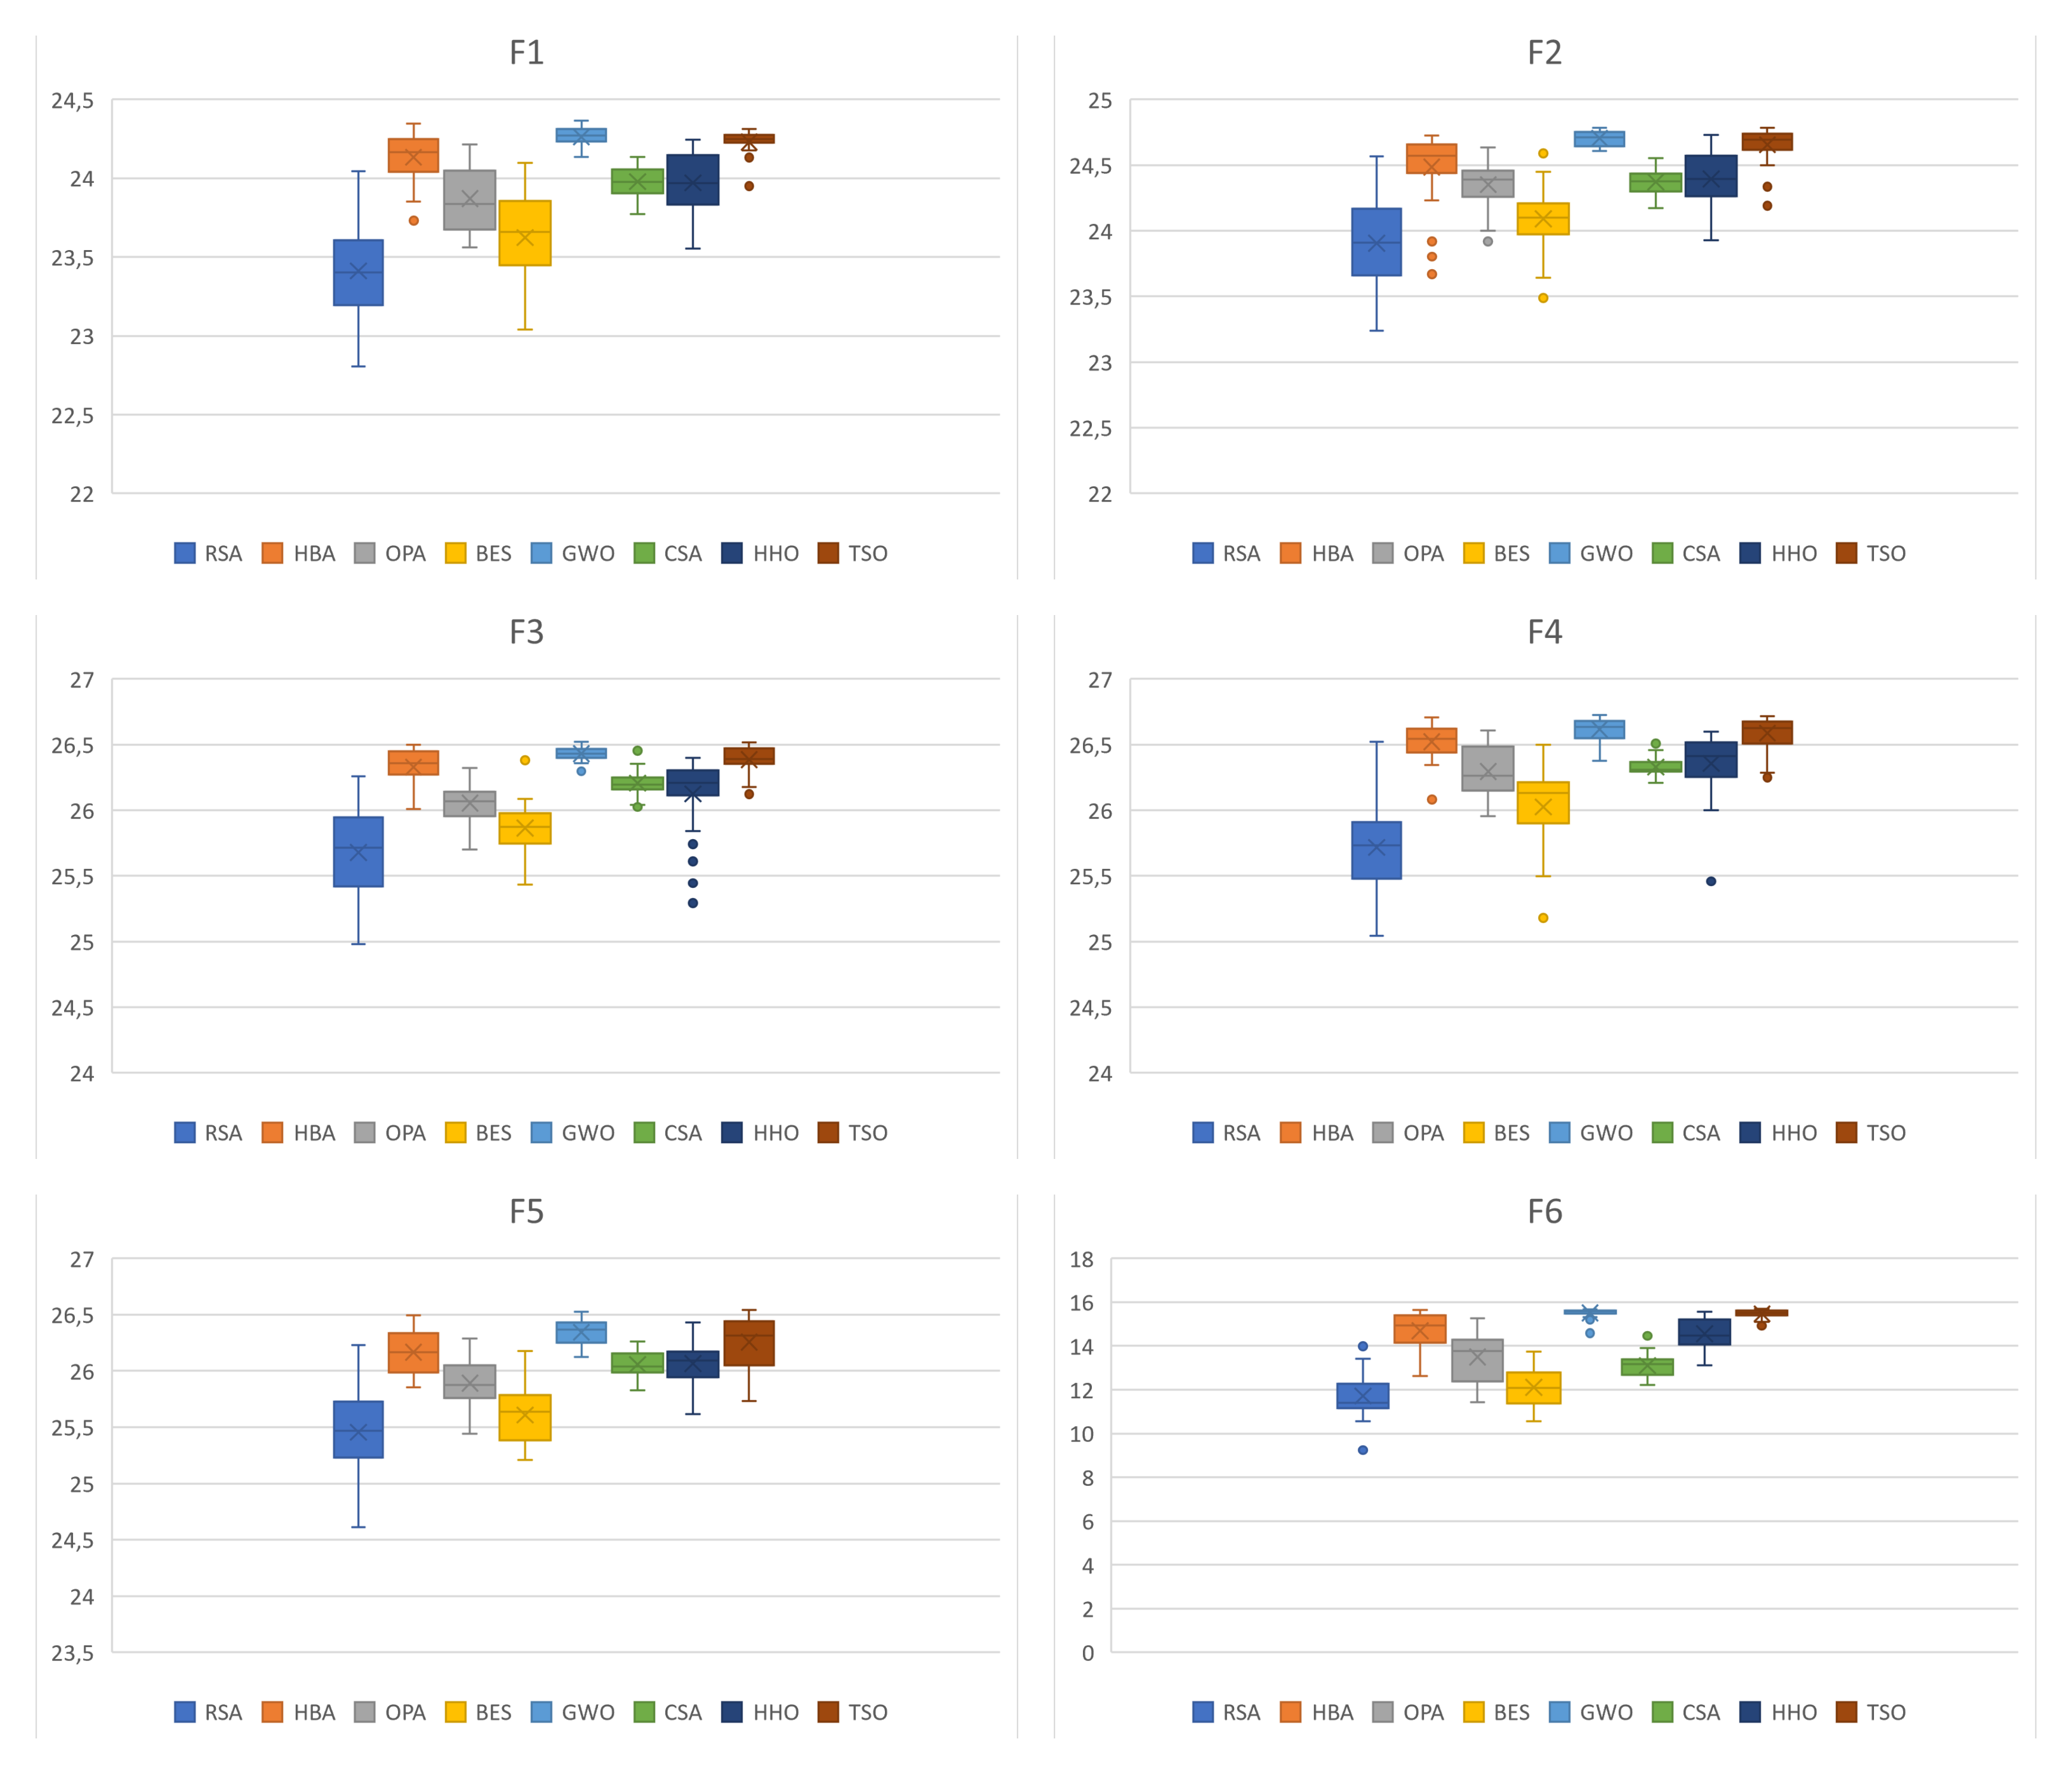
\includegraphics[width=\linewidth]{Fitness/Kapur/BoxPlot_Dim7/BoxPlots_1-6.png}
	\end{subfigure}
	
	\begin{subfigure}{0.38\textwidth}
		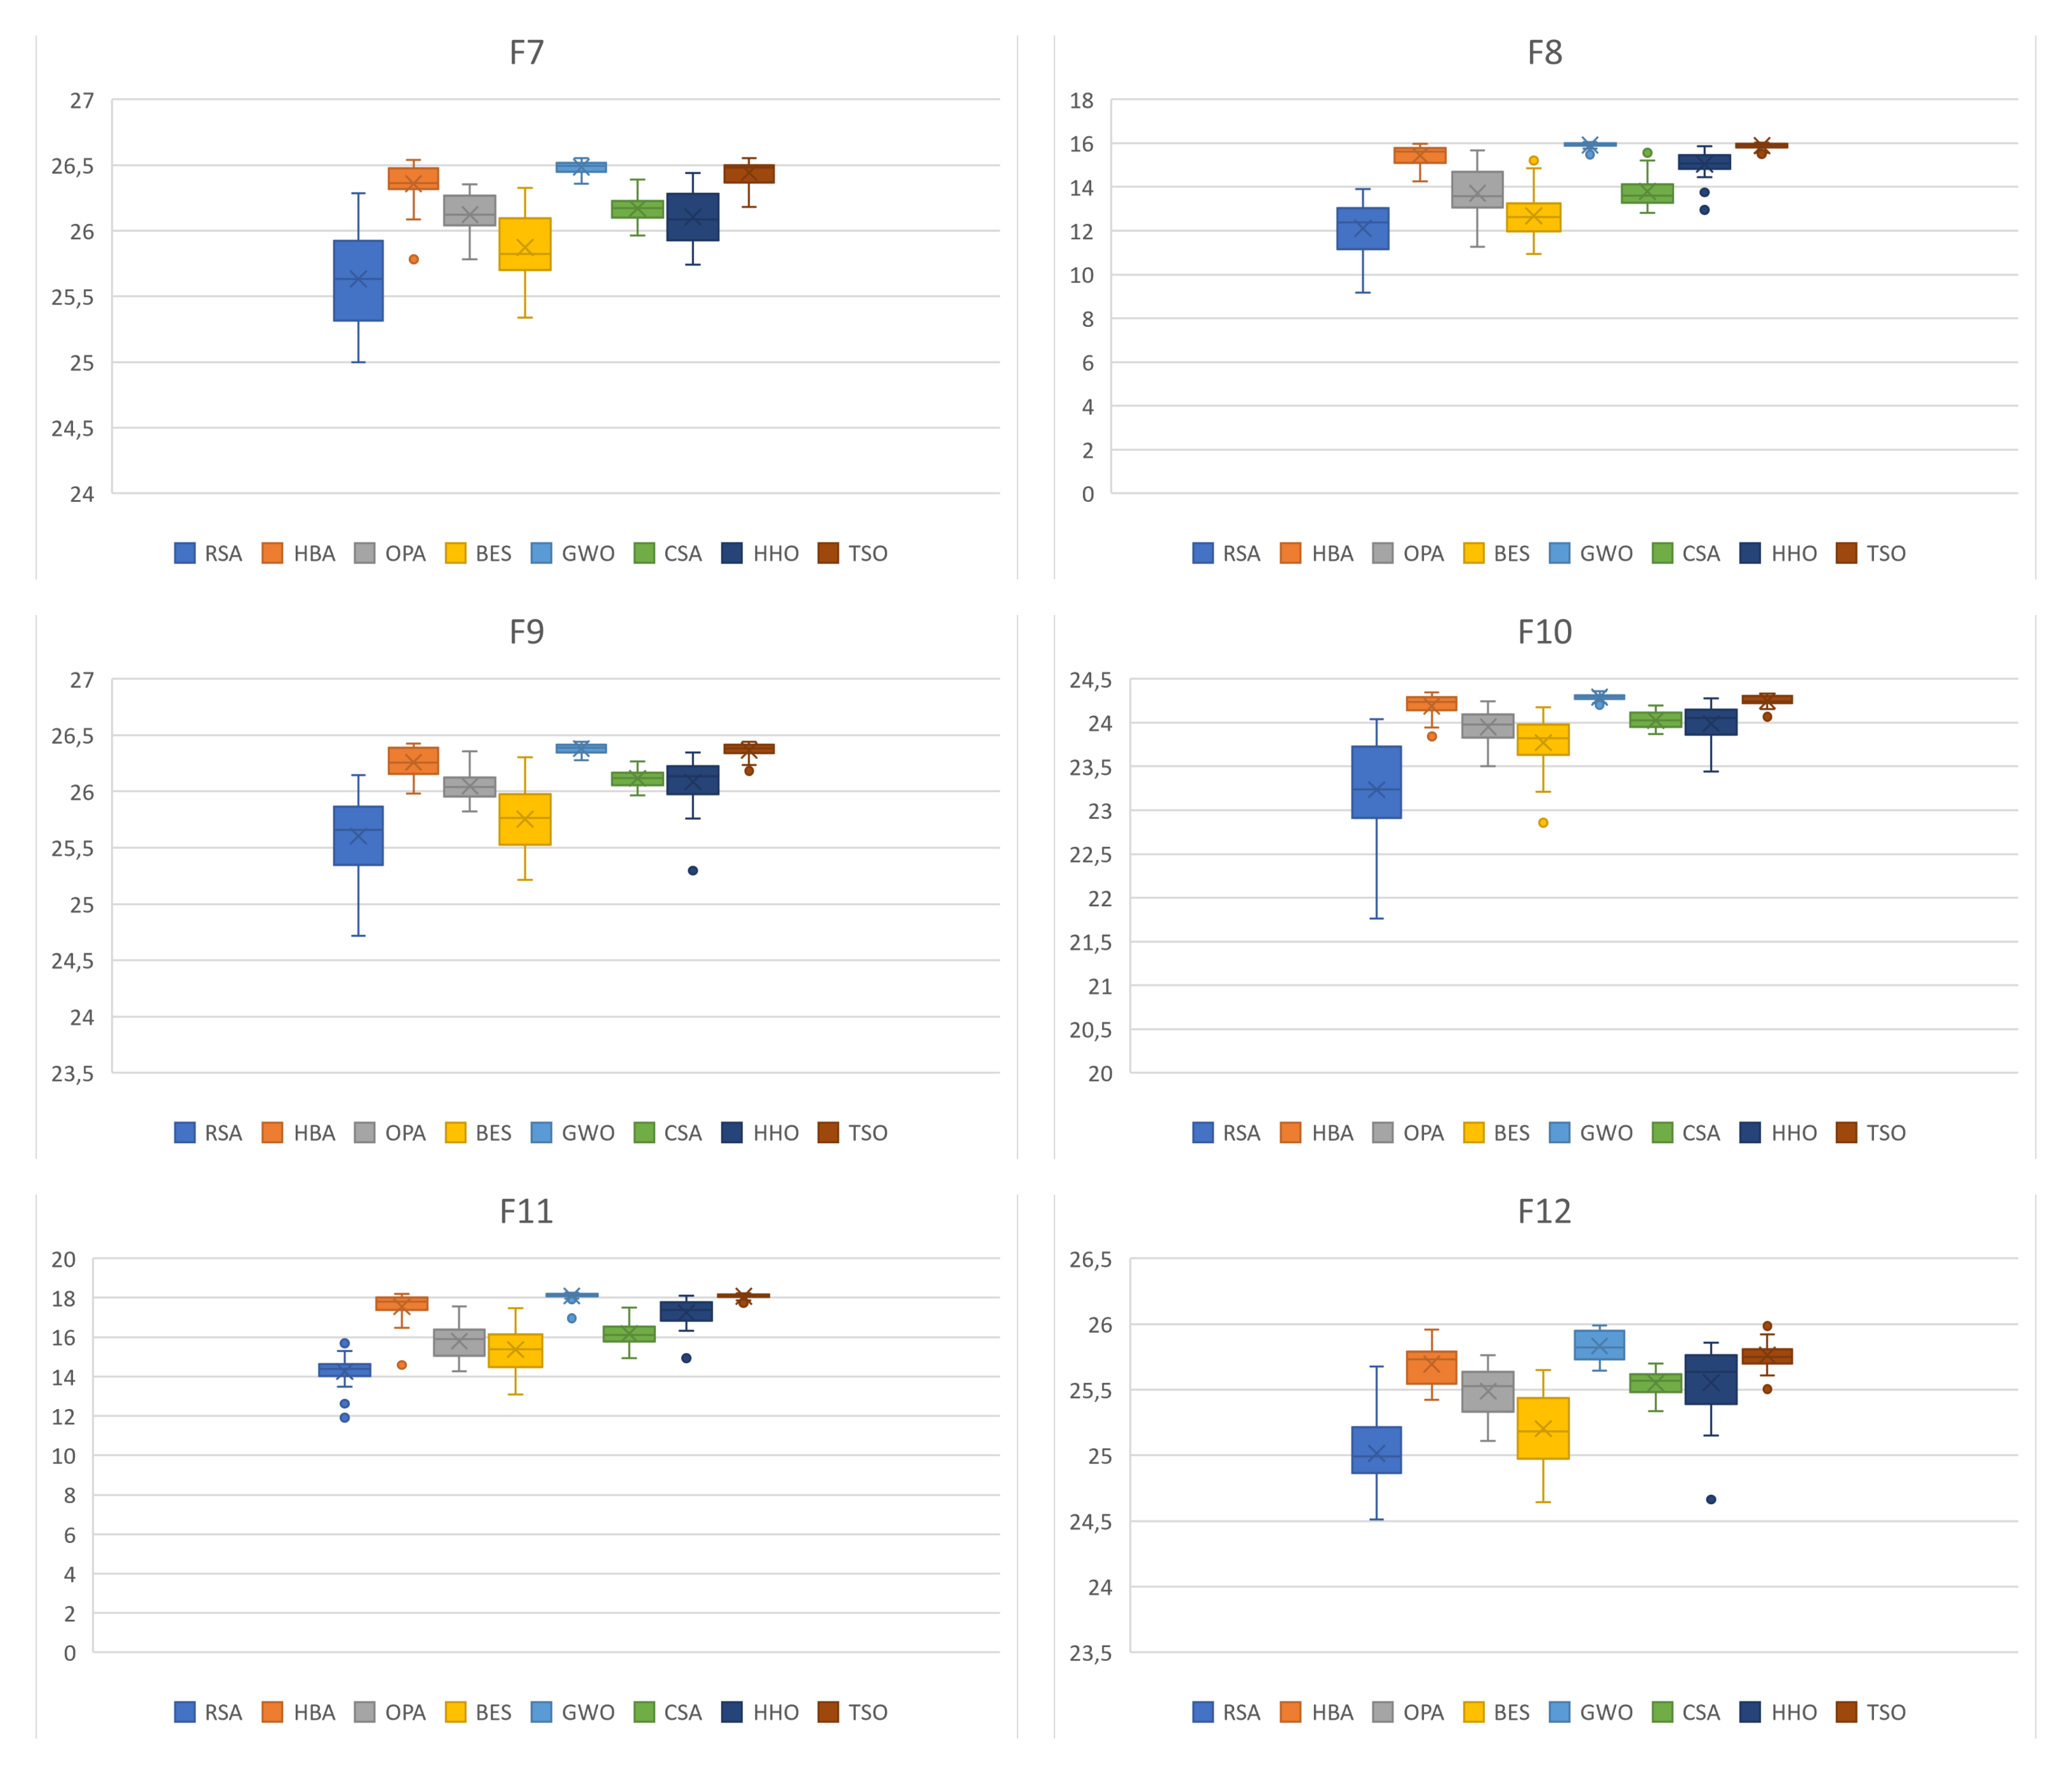
\includegraphics[width=\linewidth]{Fitness/Kapur/BoxPlot_Dim7/BoxPlots_7-12.png}
	\end{subfigure}
	\begin{subfigure}{0.38\textwidth}
		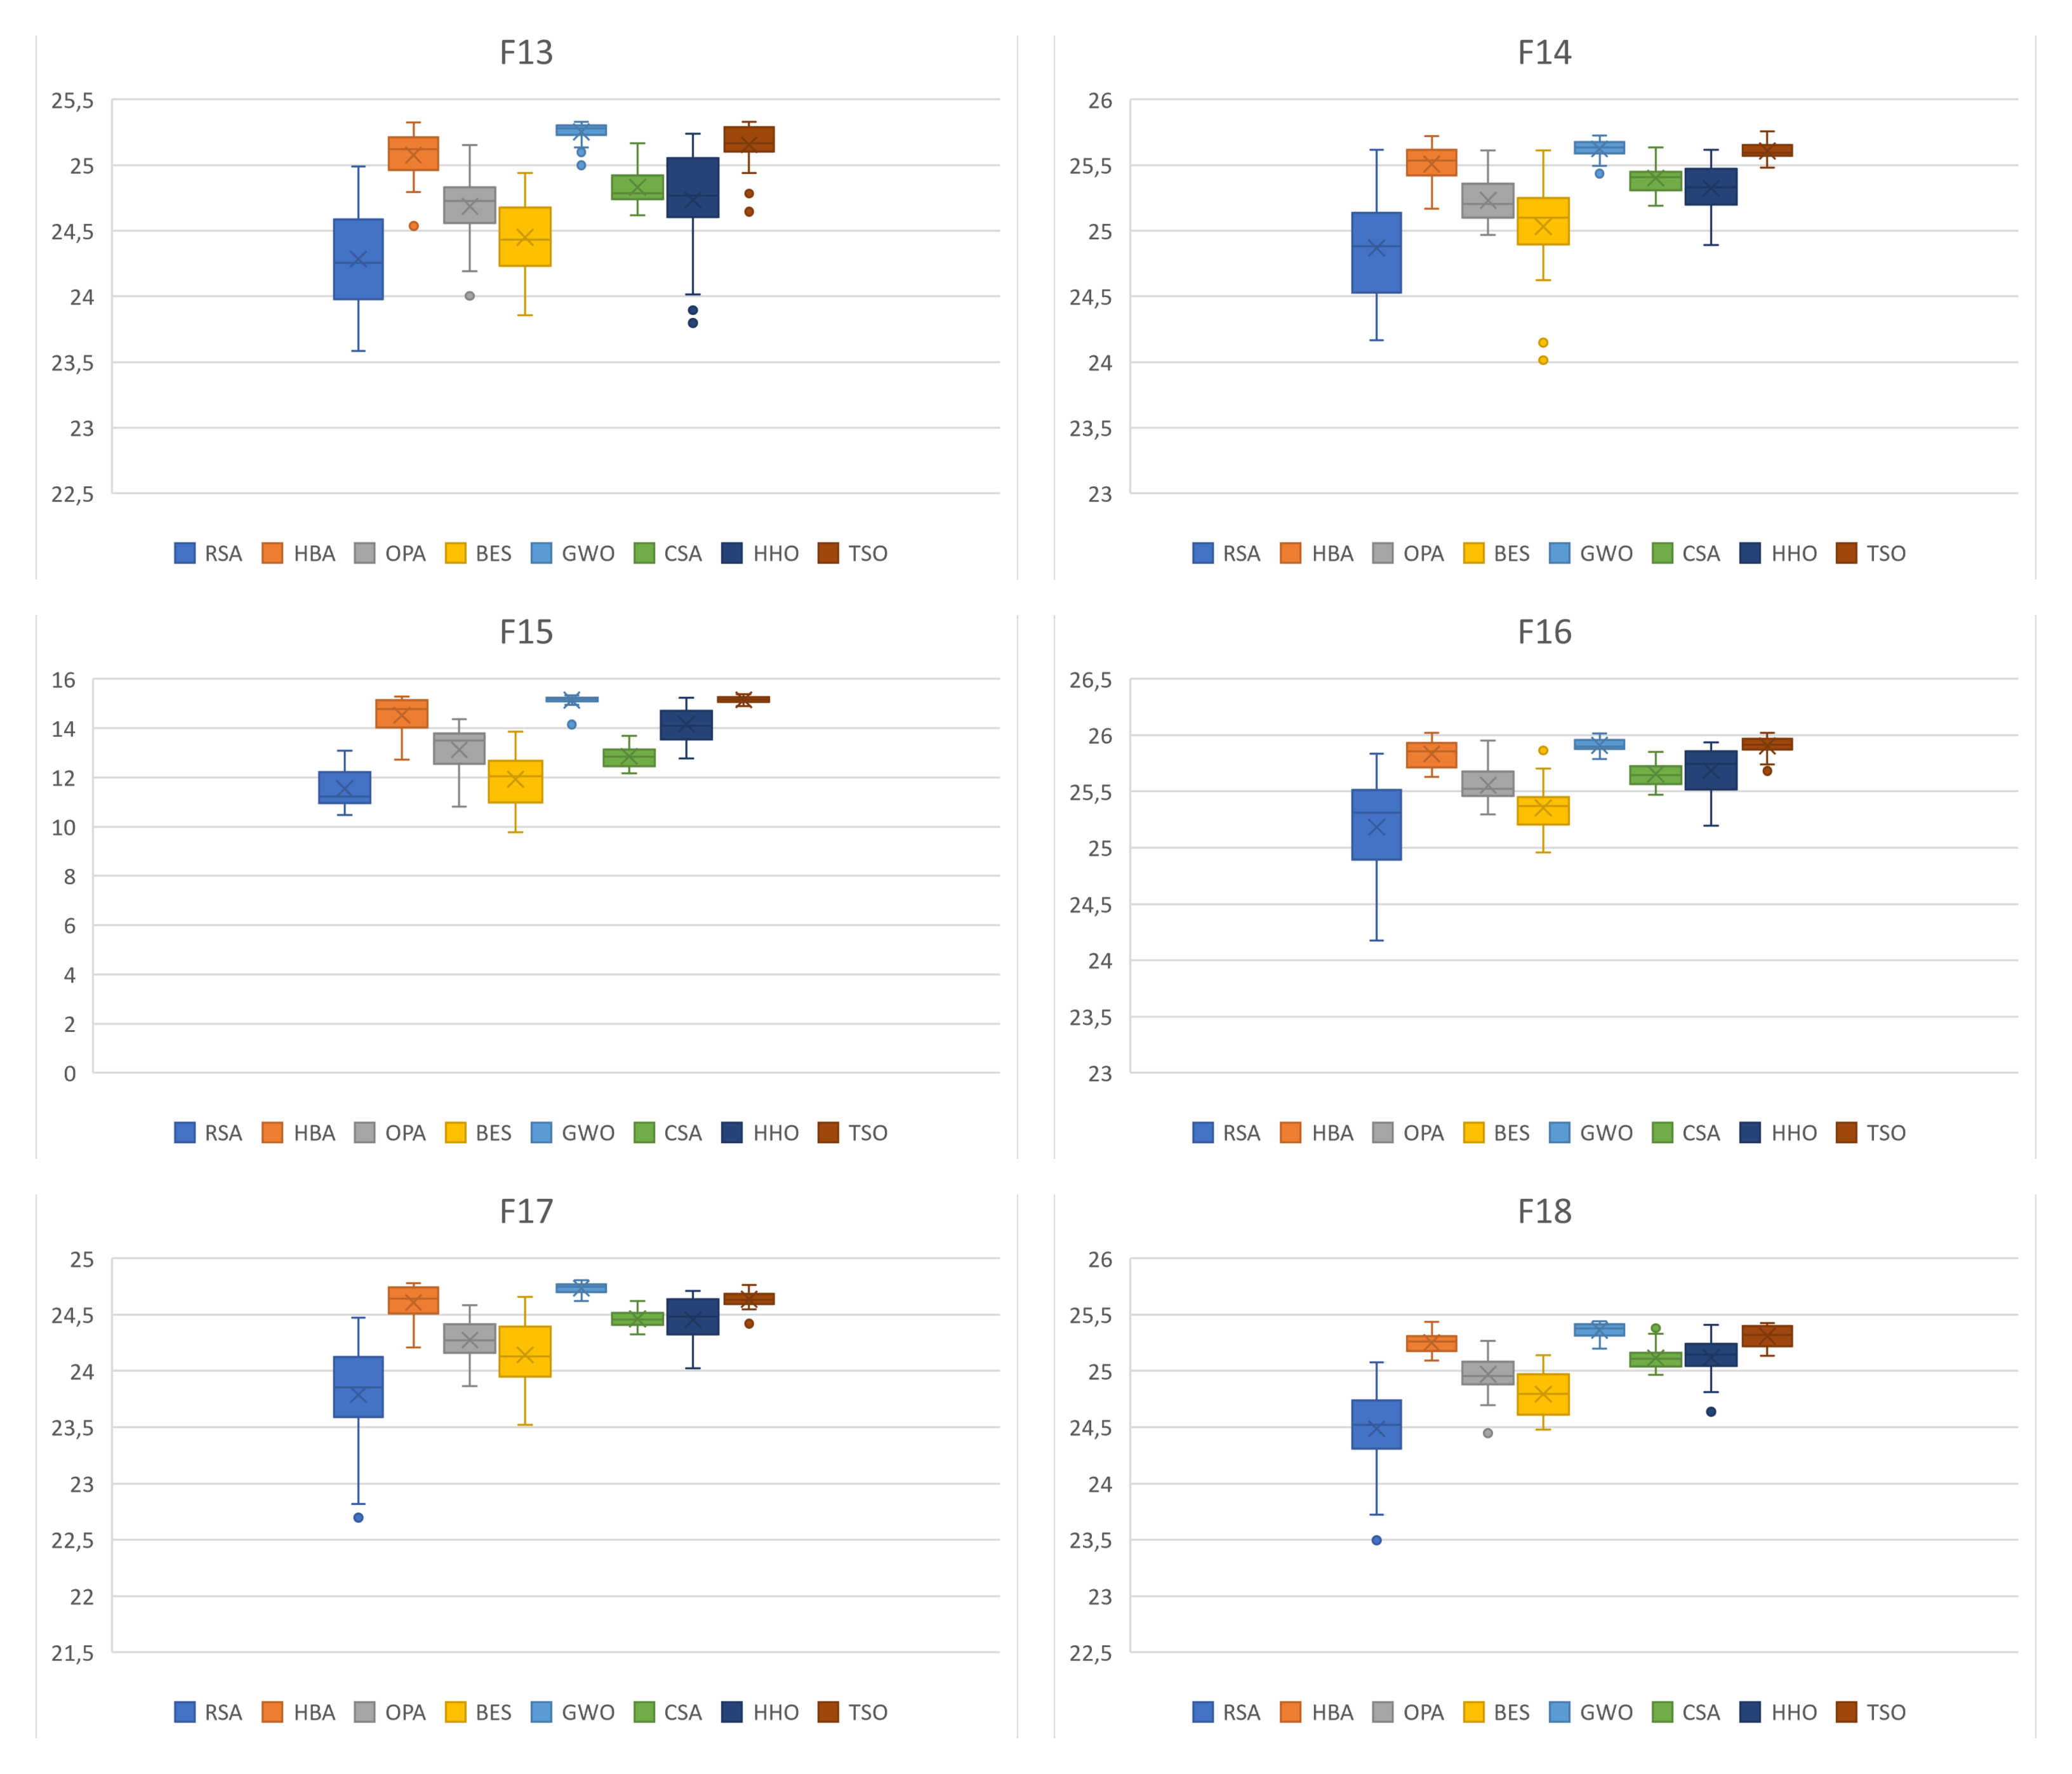
\includegraphics[width=\linewidth]{Fitness/Kapur/BoxPlot_Dim7/BoxPlots_13-18.png}
	\end{subfigure}
	\begin{subfigure}{0.38\textwidth}
		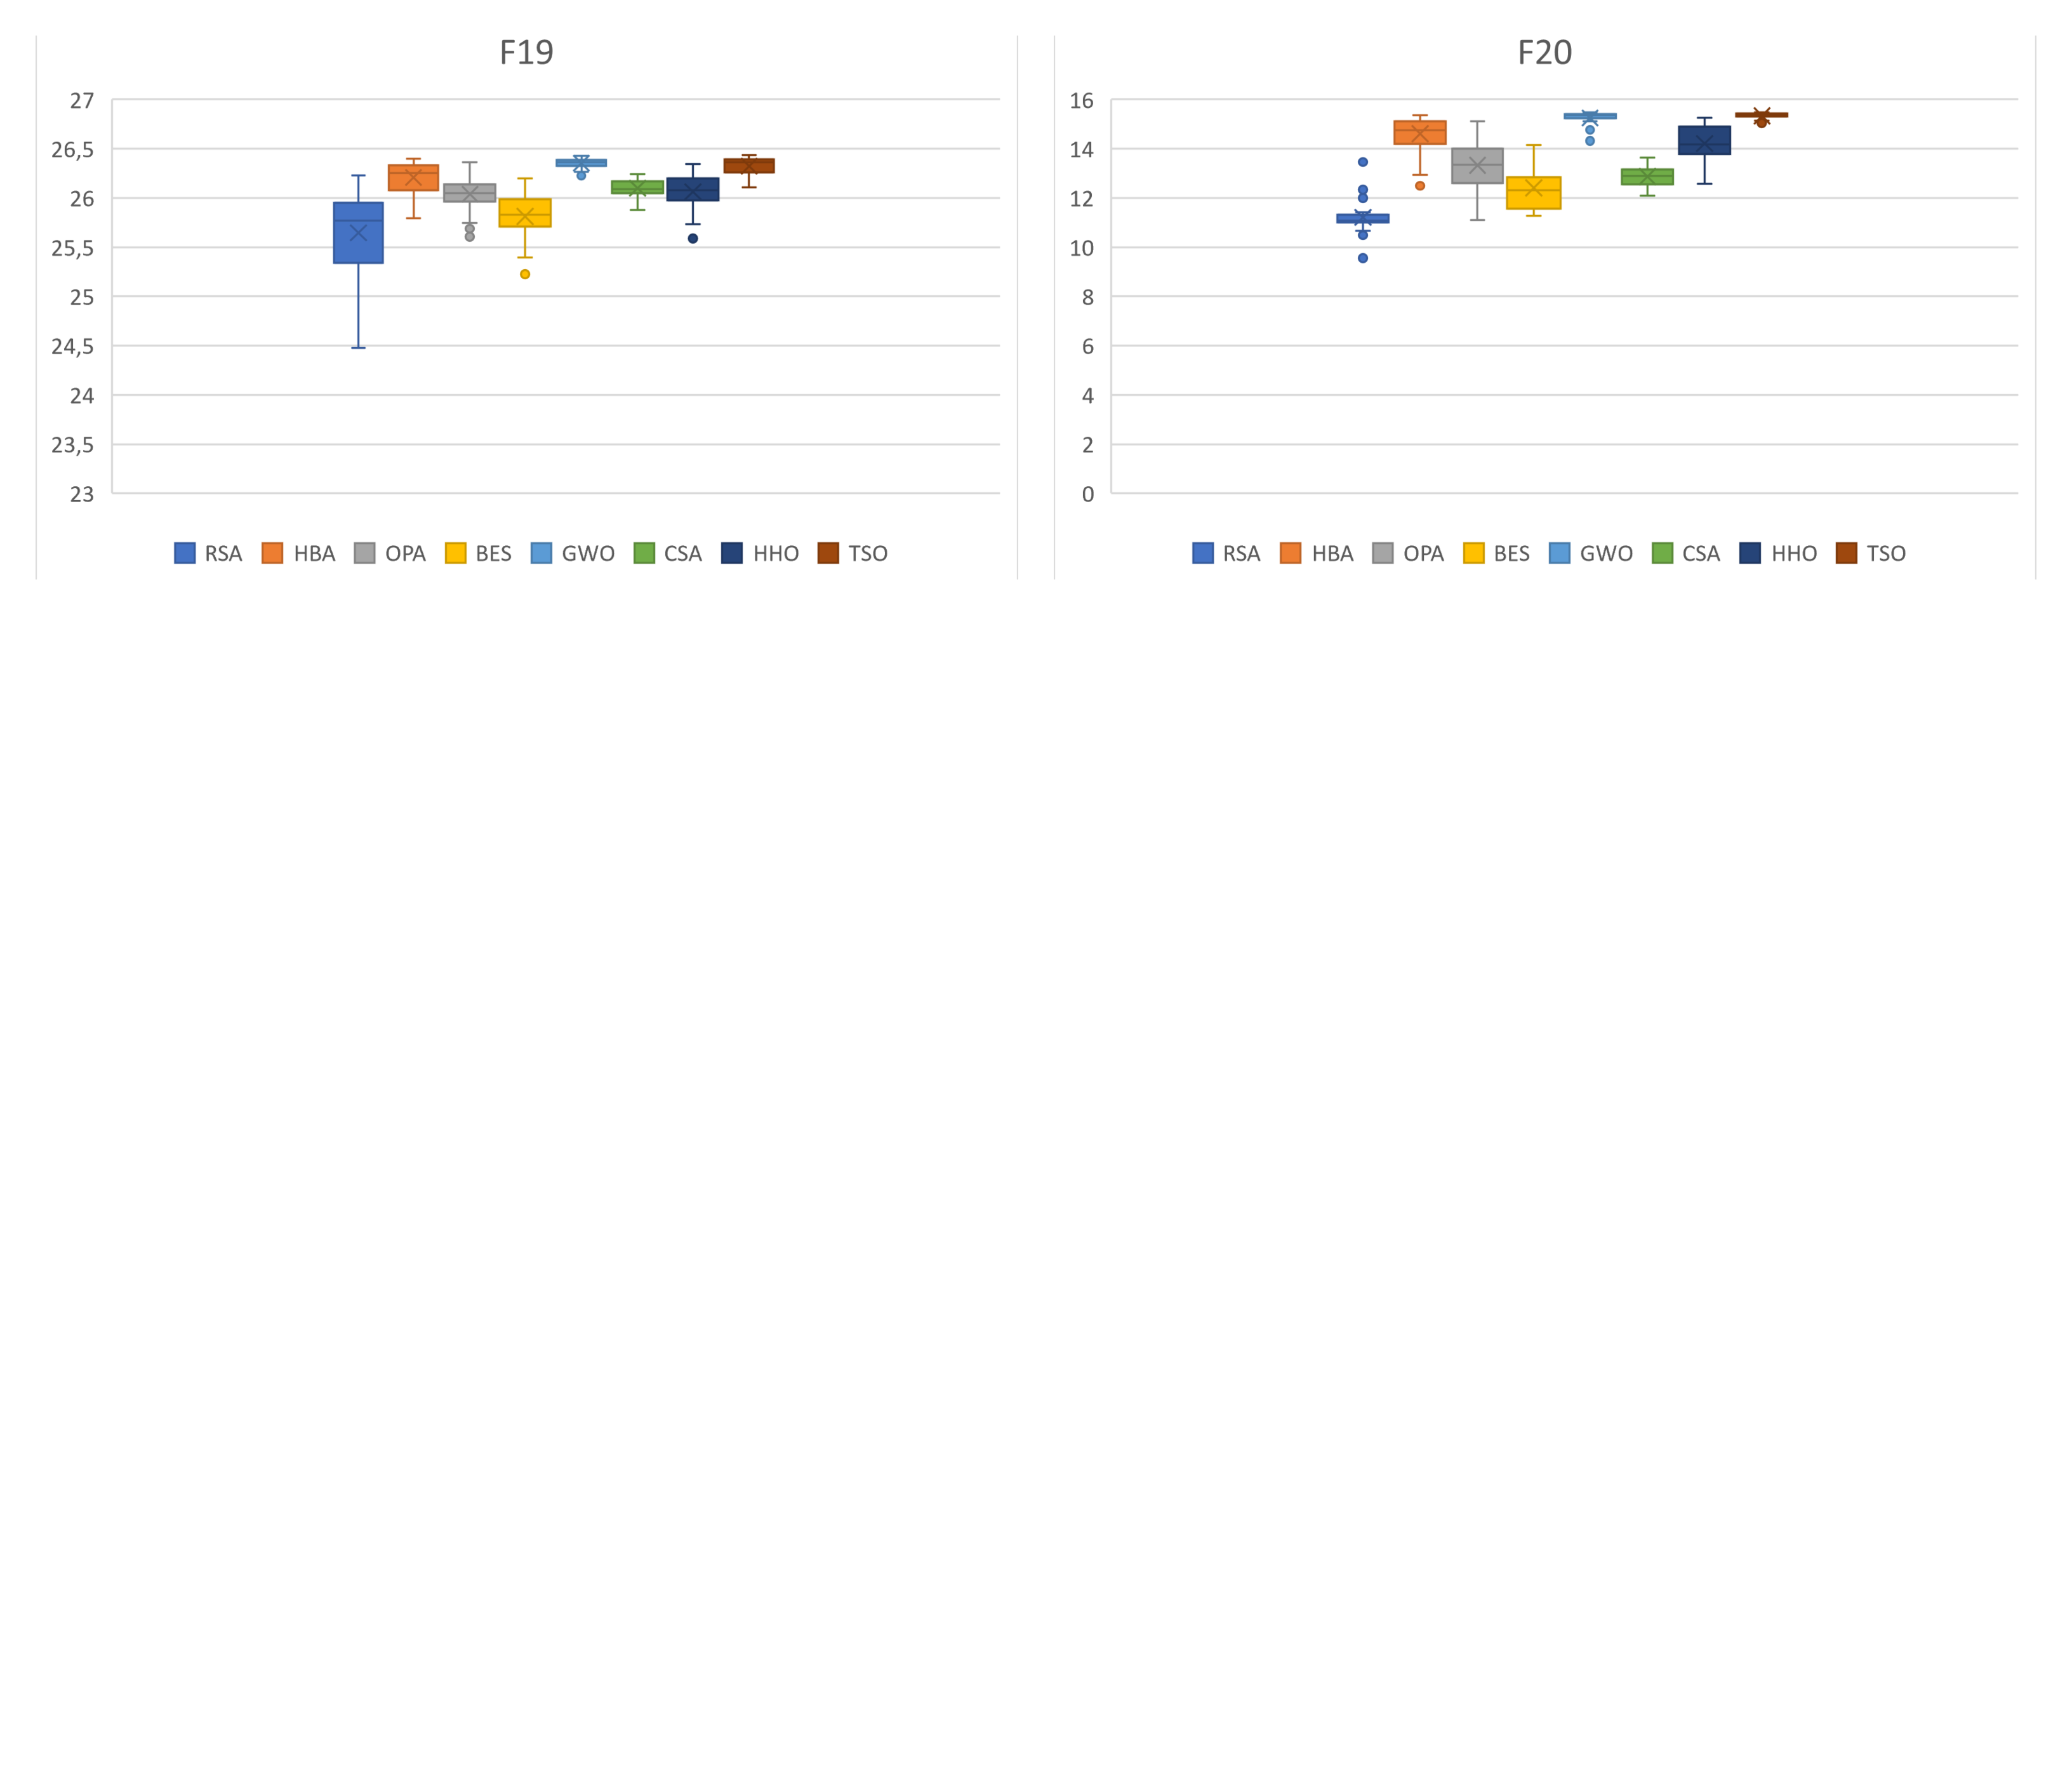
\includegraphics[width=\linewidth]{Fitness/Kapur/BoxPlot_Dim7/BoxPlots_19-20.png}
		\vspace{-120pt} % Ajusta este valor según sea necesario
	\end{subfigure}
	\caption{Boxplot de los valores Fitness por cada imagen en la dimensión 7, desde la imagen 1 hasta la imagen 20,Función Objetivo entropía de Kapur}
	\label{fig:Boxplot_Fitnes_Dim7_Kapur}    
\end{figure}

\noindent Los resultados de la función de fitness de ocho algoritmos de optimización distintos en 7 dimenciones ~\ref{fig:Boxplot_Fitnes_Dim7_Kapur}, utilizando la entropía de Kapur como función objetivo para la segmentación de imágenes, se observan patrones consistentes en el rendimiento relativo de cada algoritmo.
\begin{itemize}
	
\item GWO: Se ha mostrado consistentemente como uno de los algoritmos con mejor rendimiento. Exhibió medianas altas y rangos intercuartílicos (IQR) estrechos en la mayoría de los gráficos, lo que indica que no solo alcanza altos niveles de fitness sino que también es robusto y confiable en sus resultados.

\item CSA y HHO: Ambos algoritmos también mostraron un rendimiento fuerte y consistente a través de las diferentes evaluaciones. Sus medianas se mantuvieron altas y los IQR estrechos, reafirmando su eficacia y estabilidad como métodos de optimización.

\item RSA: Tendió a tener un rendimiento más bajo en comparación con los demás algoritmos. Aunque su IQR a veces era estrecho, lo que sugiere cierta consistencia, sus medianas eran generalmente más bajas y presentaba valores atípicos que indicaban resultados significativamente peores en algunos casos.

\item HBA, OPA, BES y TSO: Estos algoritmos mostraron un rendimiento medio, con medianas que generalmente se encontraban en el centro del rango y IQR que indicaban una variabilidad de moderada a alta. Ninguno de estos se destacó consistentemente como el mejor o el peor después del RSA, pero sus resultados no fueron tan robustos como los del GWO, CSA y HHO.
\end{itemize}

\noindent El mejor algoritmo: Basado en el análisis general, el GWO se destaca como el mejor algoritmo debido a su alto rendimiento y consistencia en todas las evaluaciones.

\noindent El peor algoritmo: El RSA parece ser el algoritmo con peor rendimiento debido a sus medianas más bajas y presencia de resultados atípicos que sugieren una mayor probabilidad de obtener resultados de optimización pobres.
\subsubsection{Dimensión 8}
% Dimension 8
\begin{figure}
	\centering
	
	\begin{subfigure}{0.415\textwidth}
		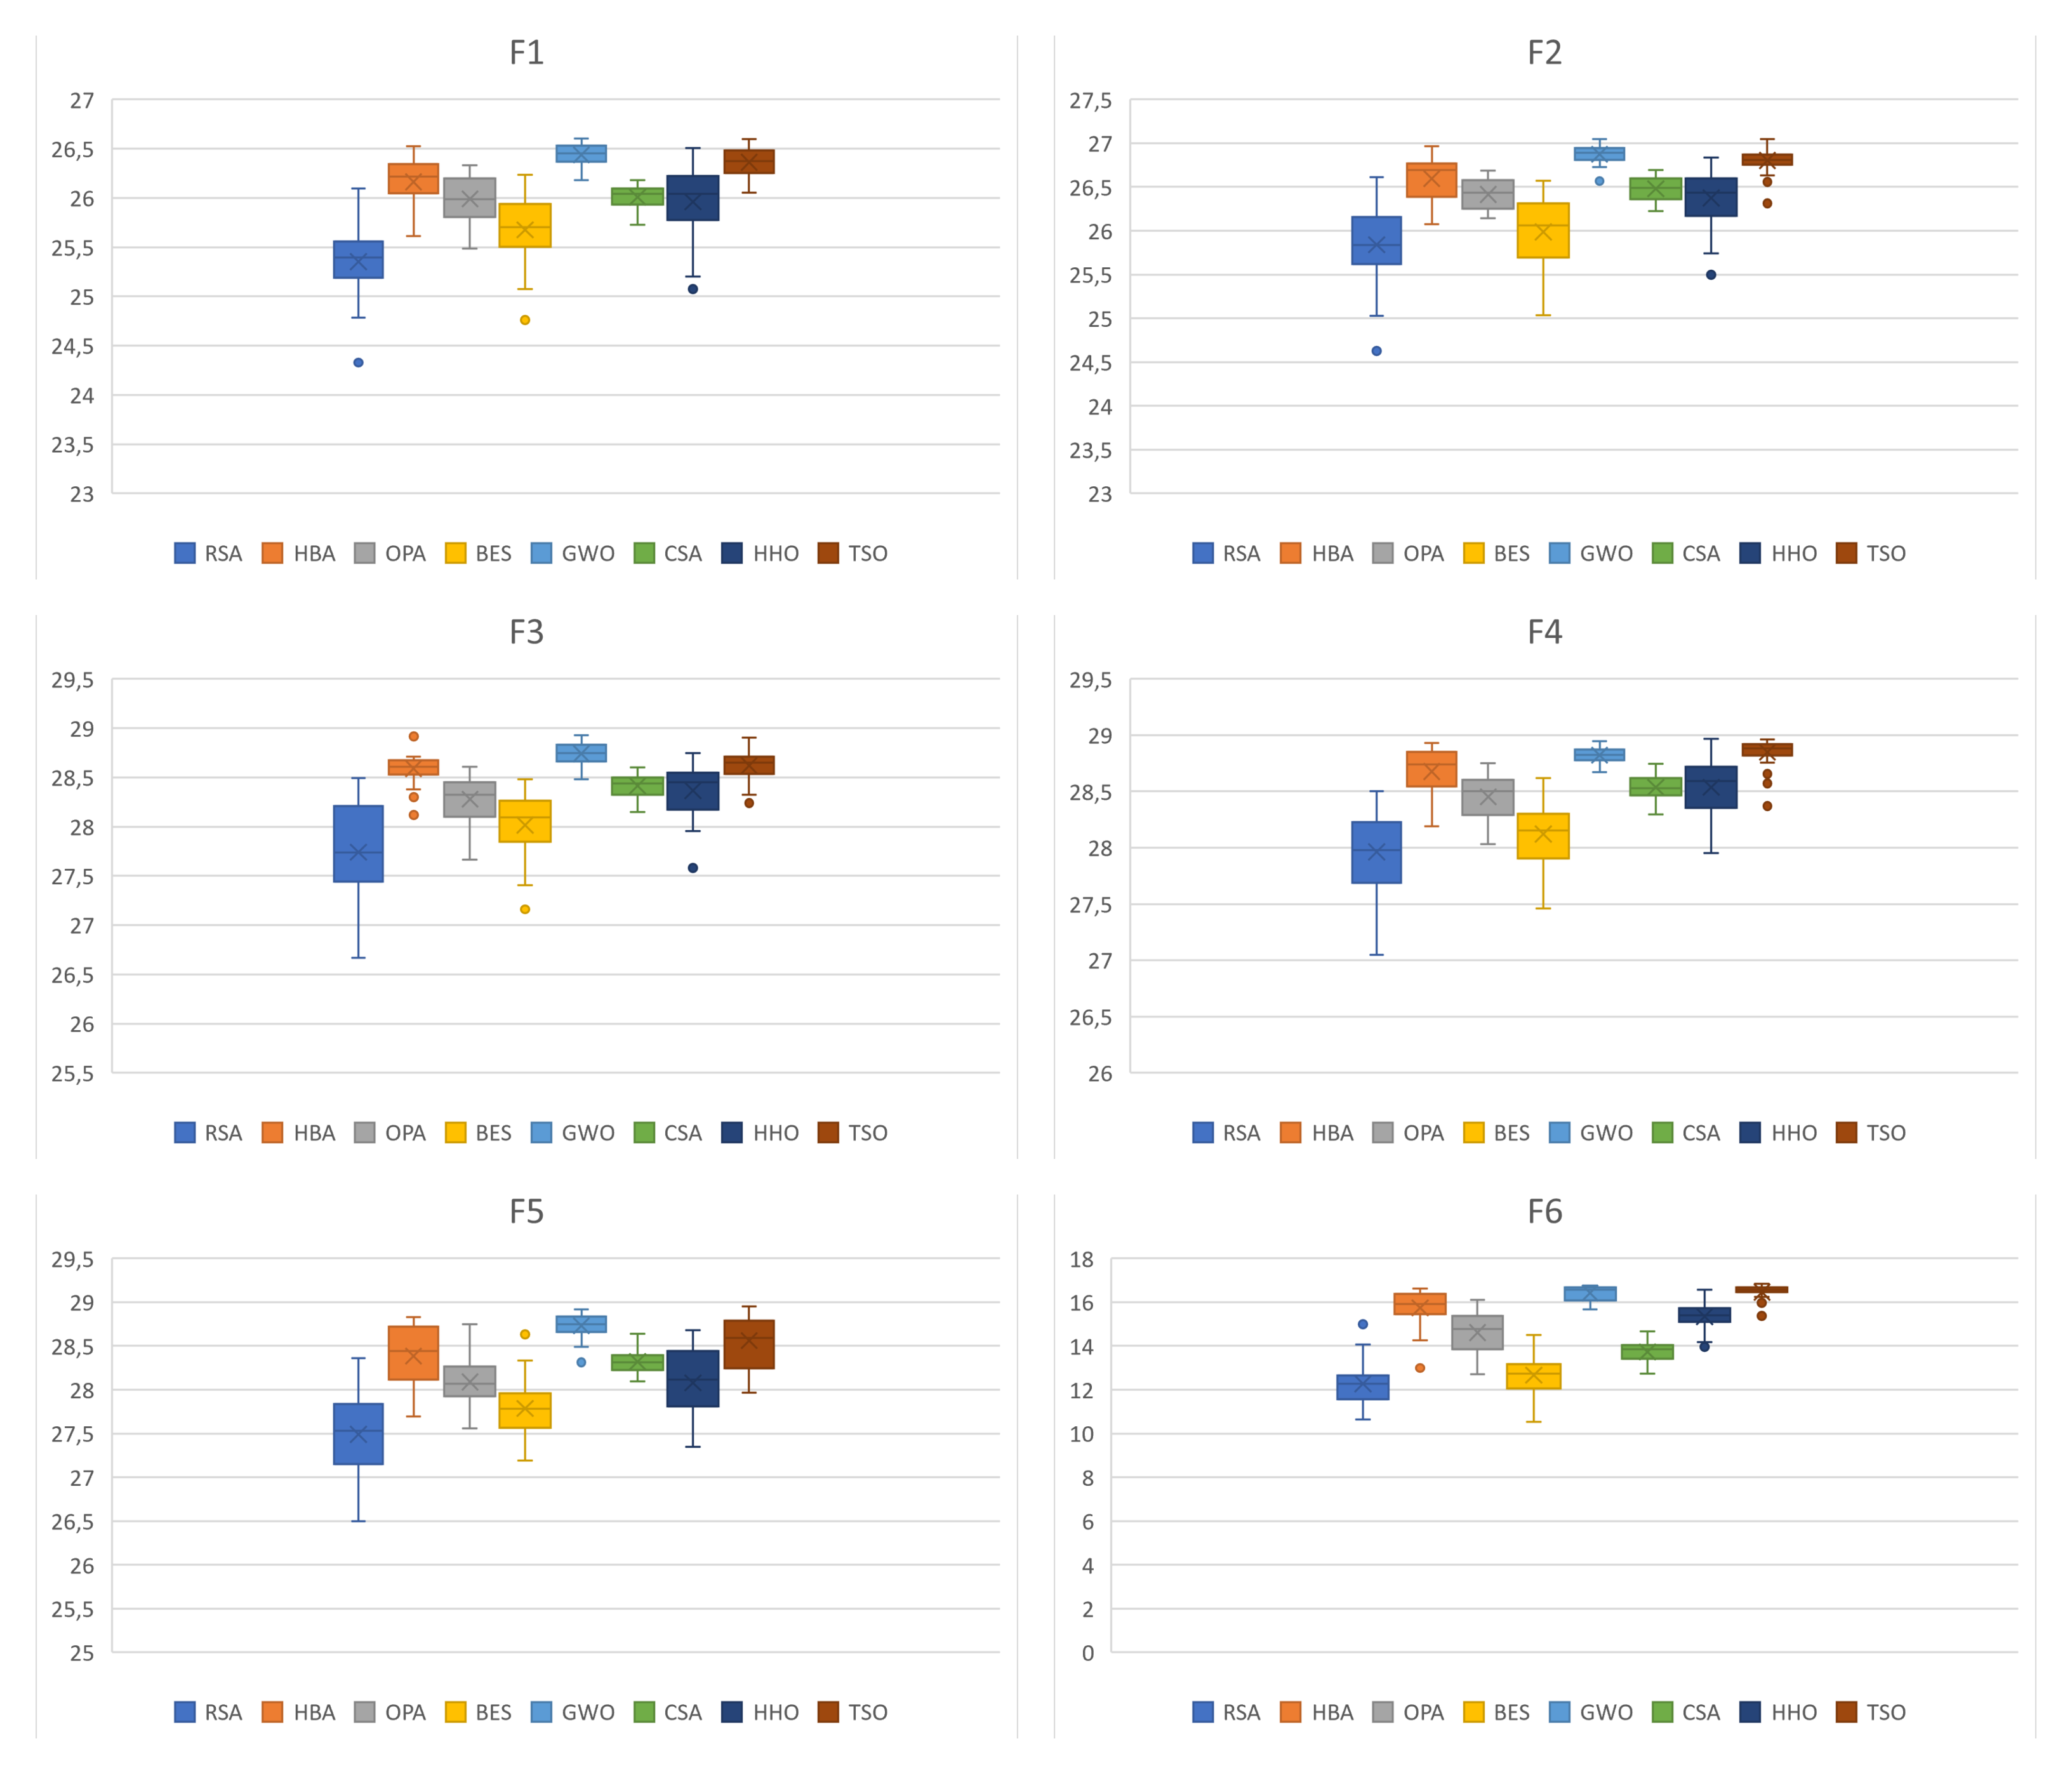
\includegraphics[width=\linewidth]{Fitness/Kapur/BoxPlot_Dim8/BoxPlots_1-6_Dim8.png}
	\end{subfigure}
	
	\begin{subfigure}{0.415\textwidth}
		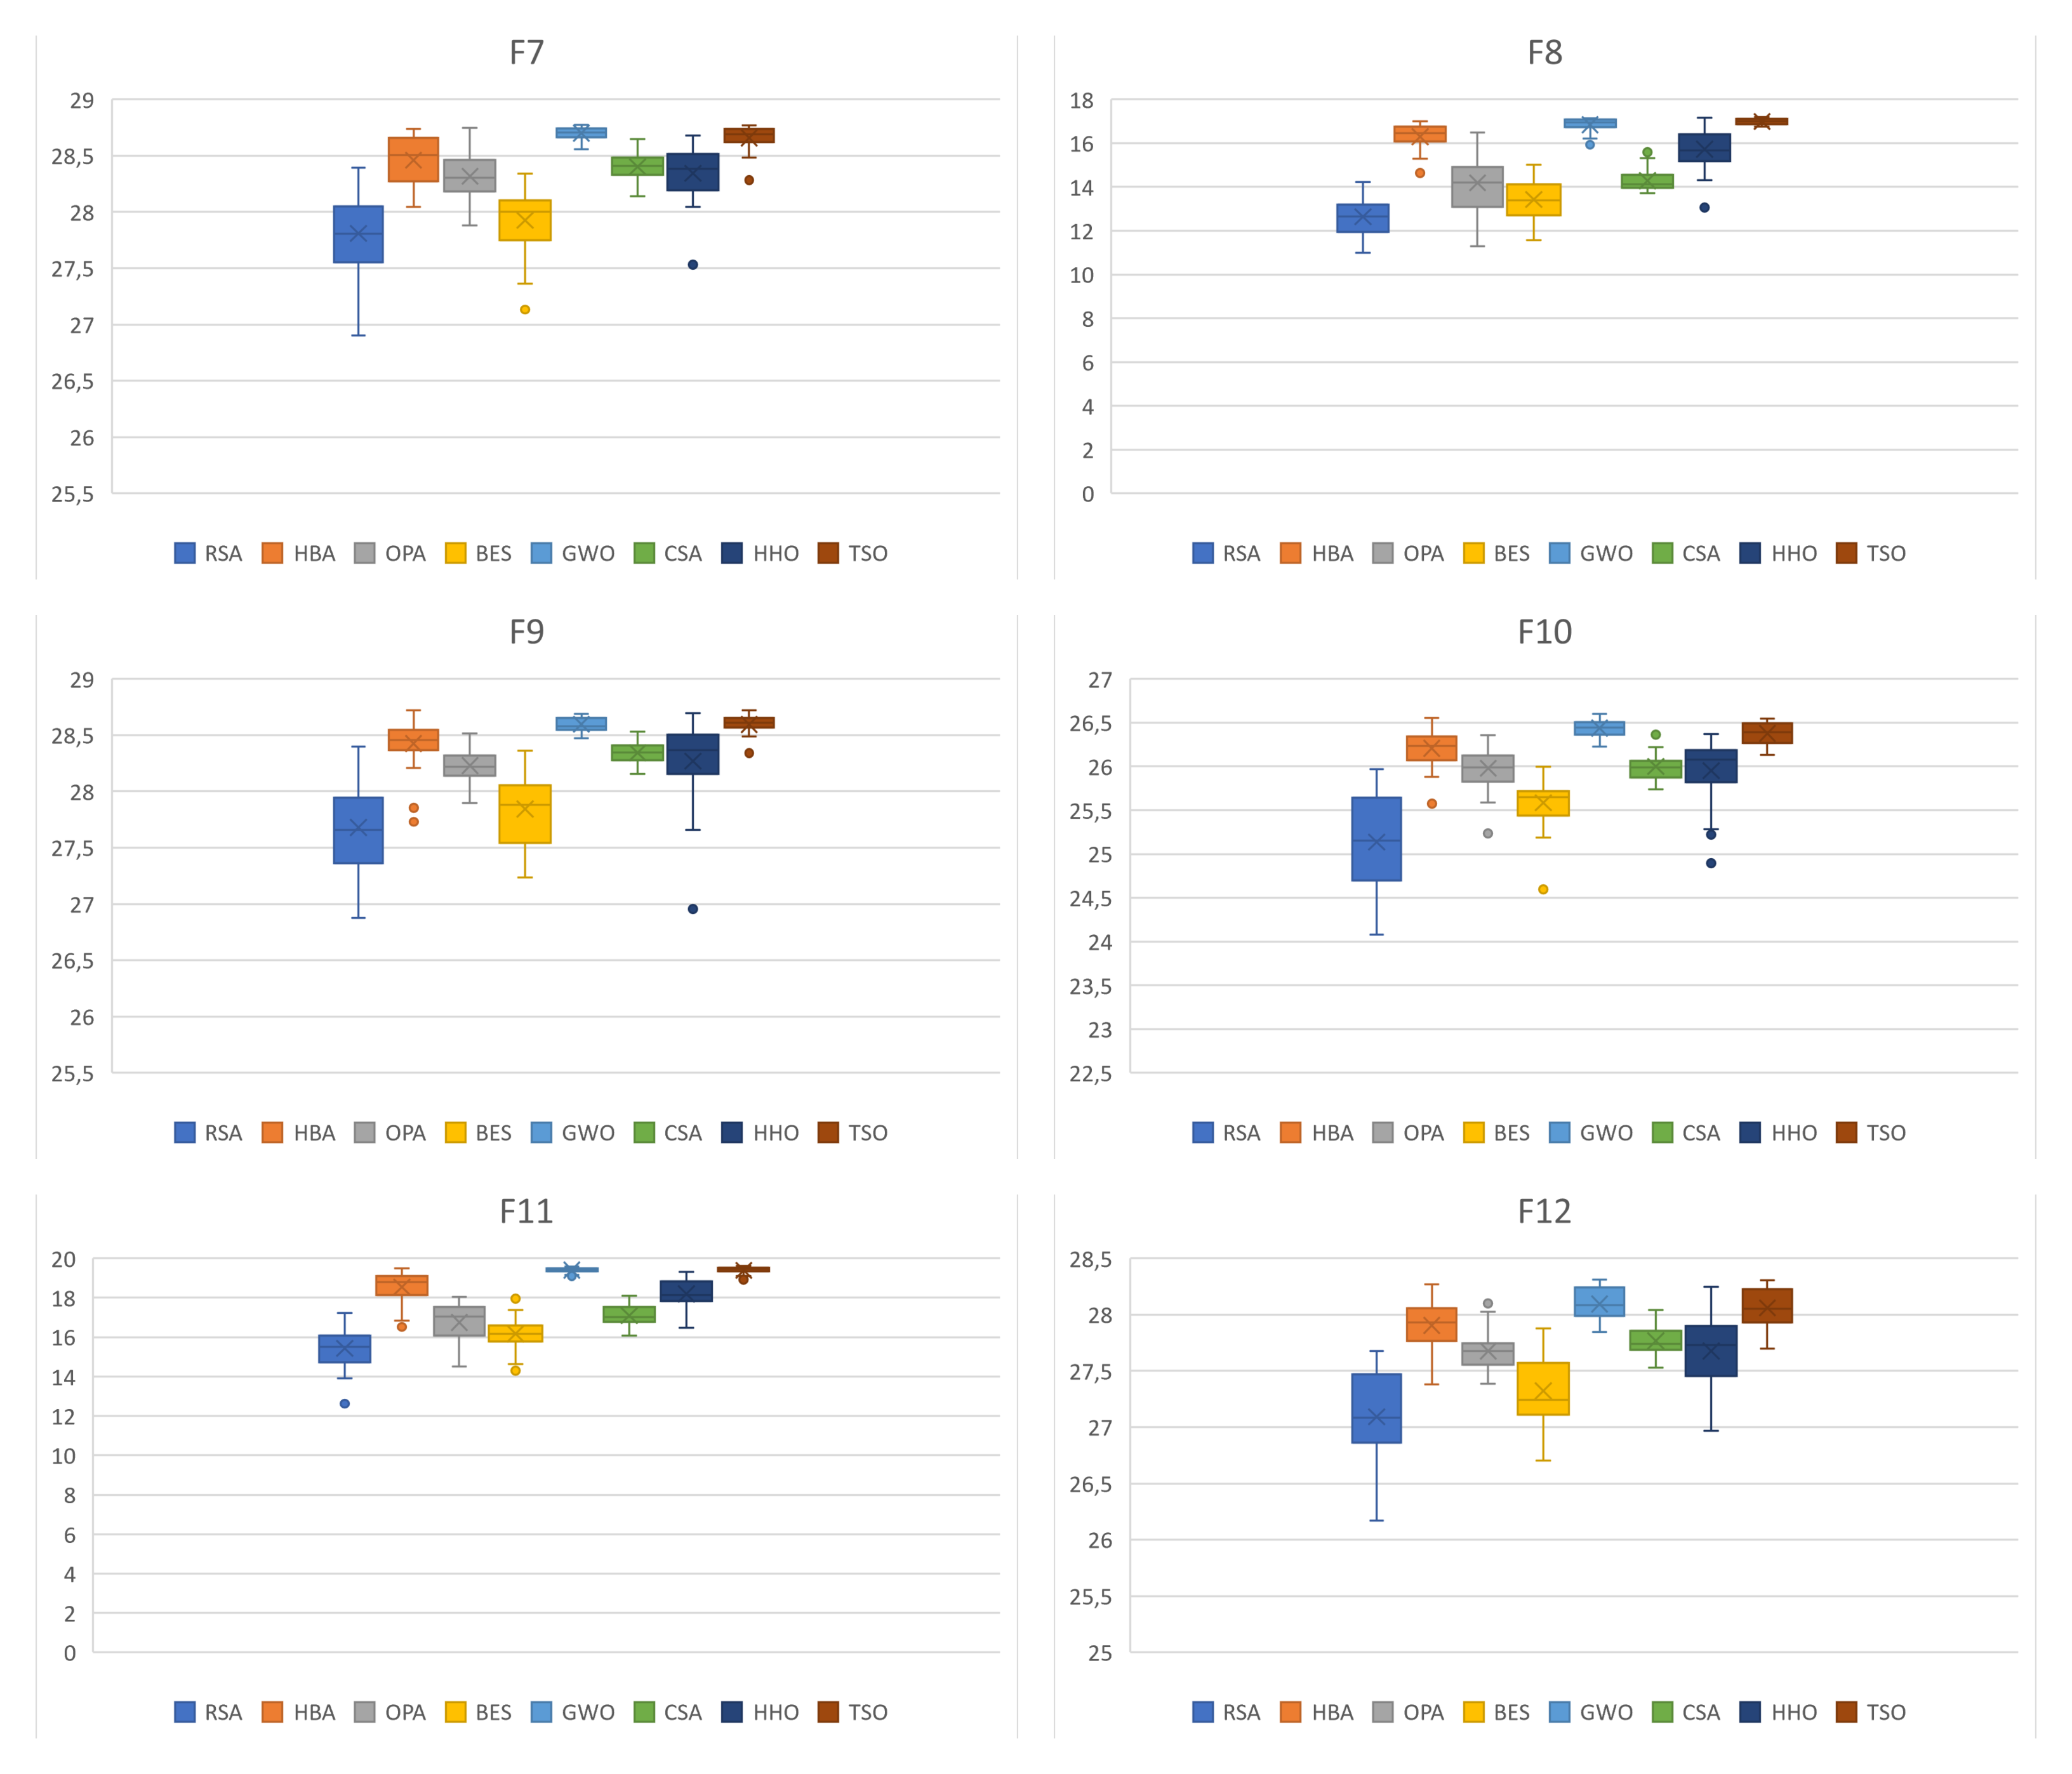
\includegraphics[width=\linewidth]{Fitness/Kapur/BoxPlot_Dim8/BoxPlots_7-12_Dim8.png}
	\end{subfigure}
	\begin{subfigure}{0.415\textwidth}
		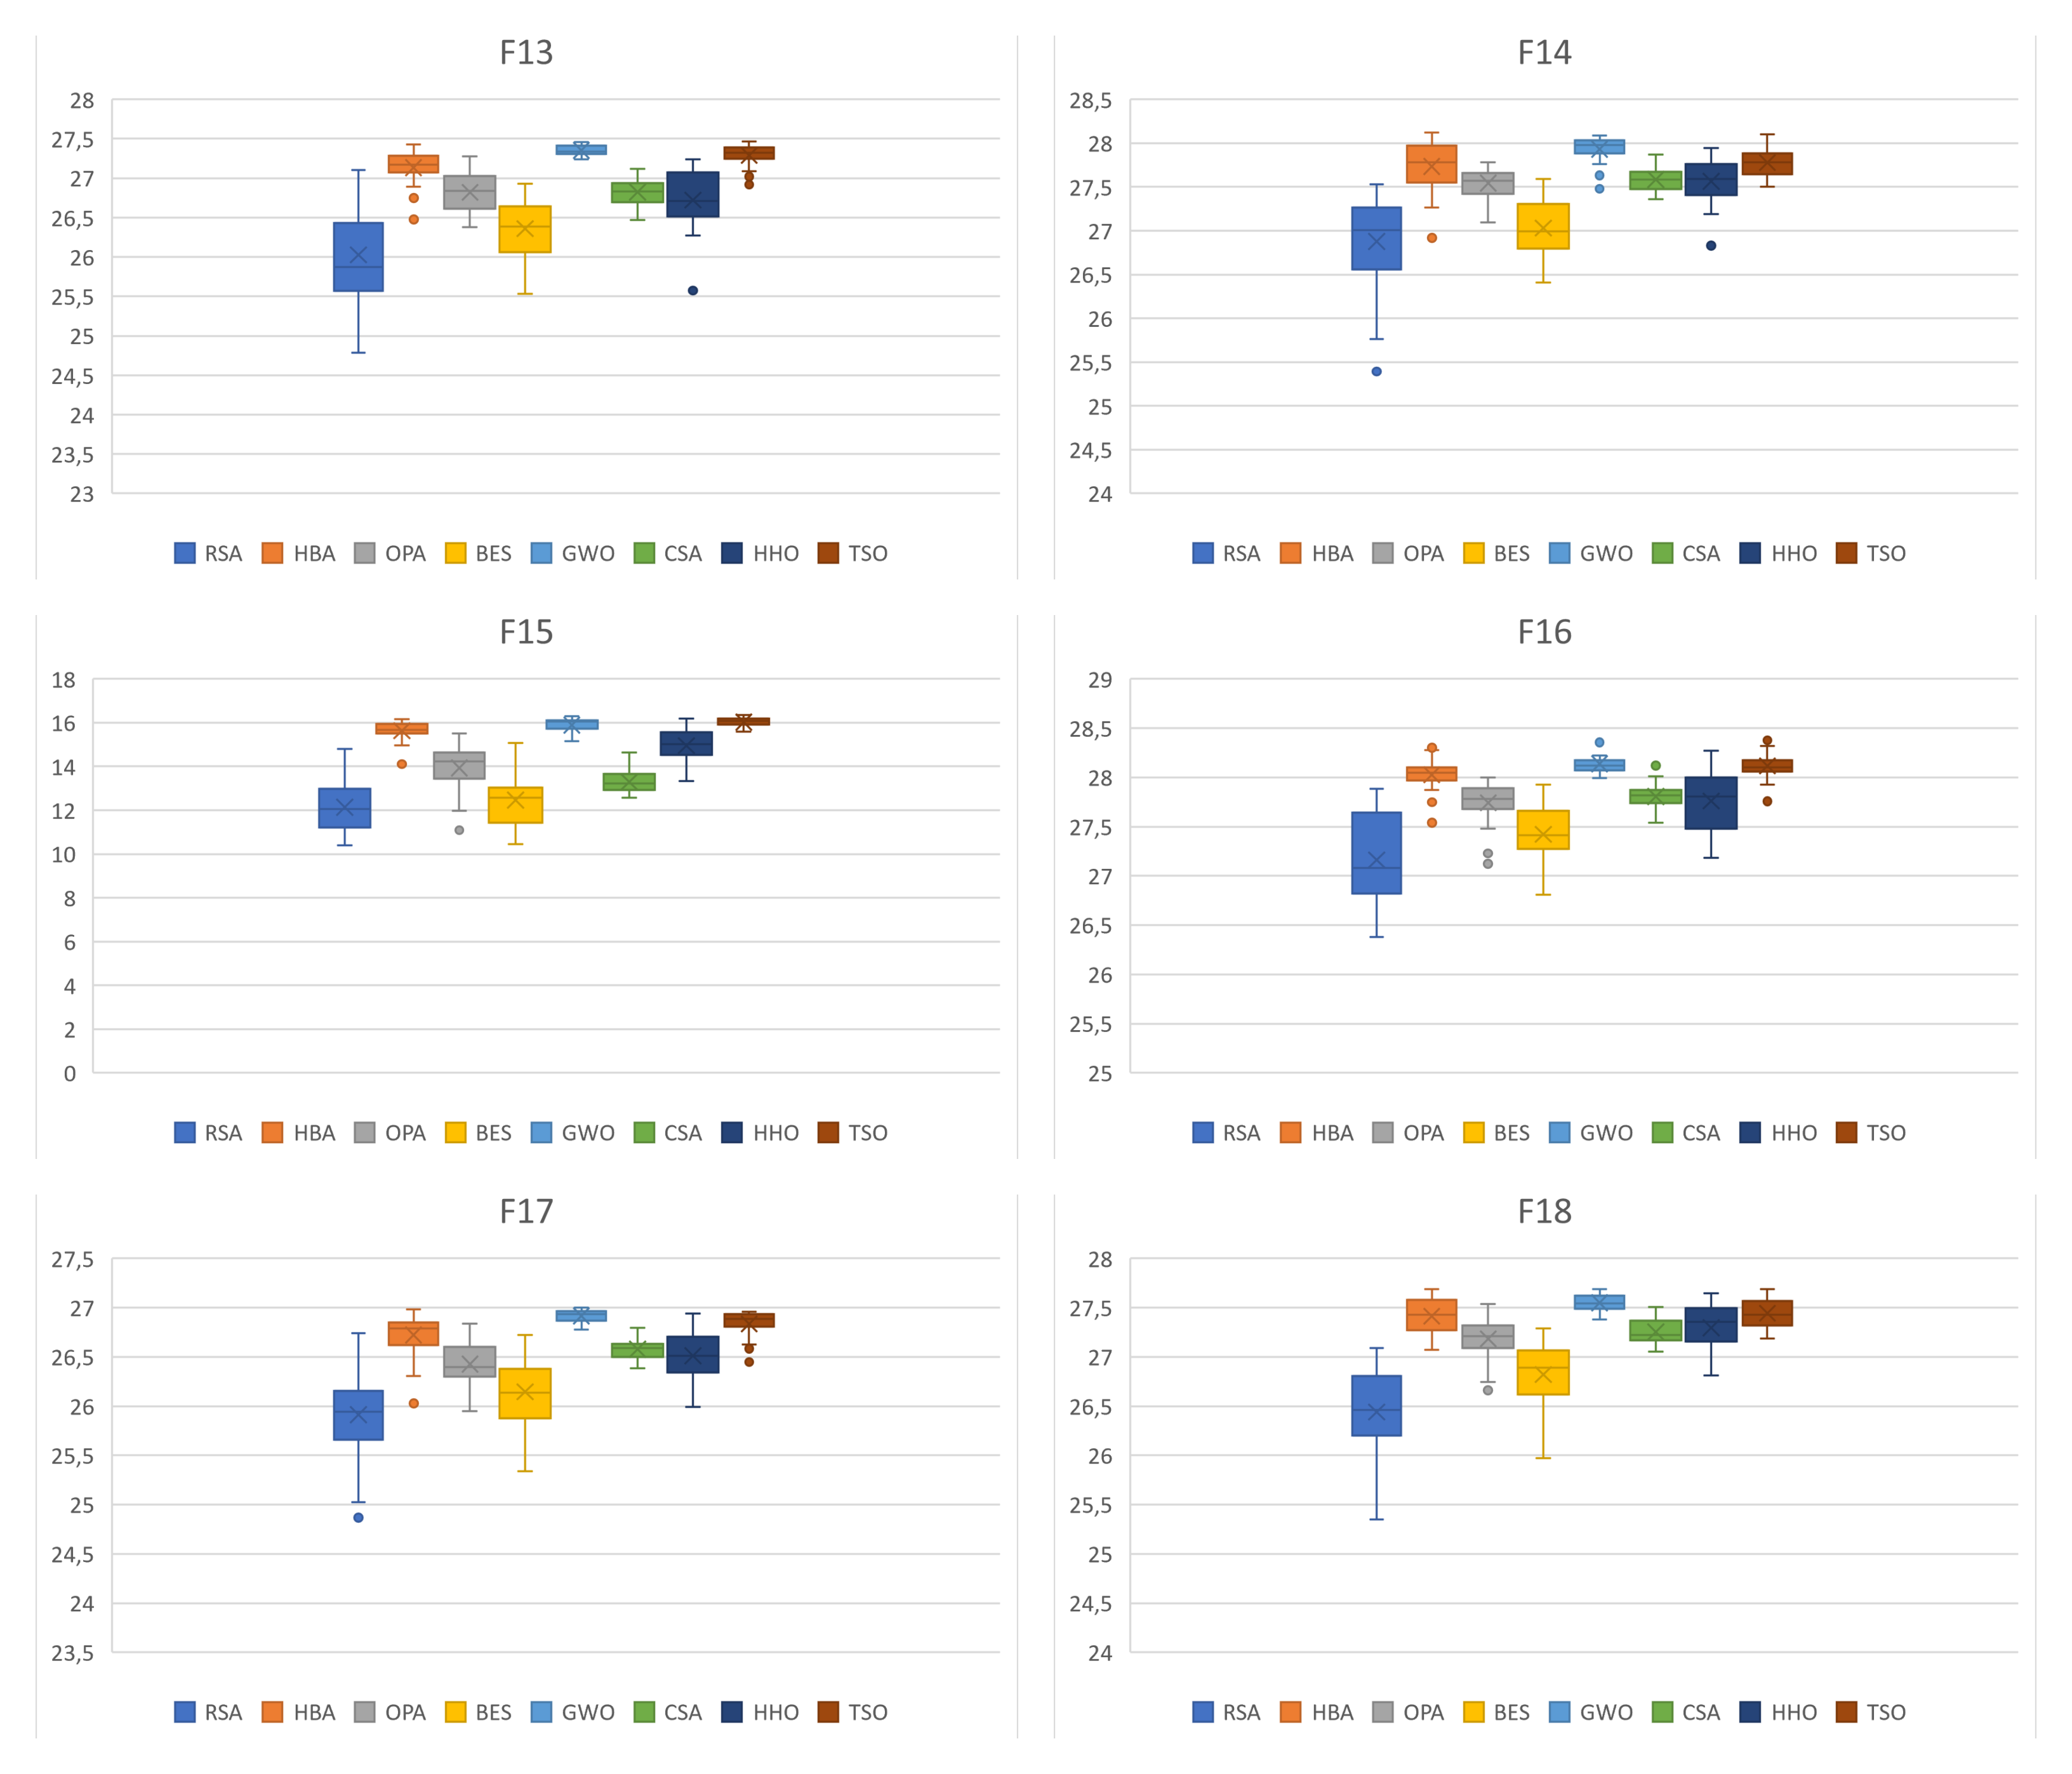
\includegraphics[width=\linewidth]{Fitness/Kapur/BoxPlot_Dim8/BoxPlots_13-18_Dim8.png}
	\end{subfigure}
	\begin{subfigure}{0.415\textwidth}
		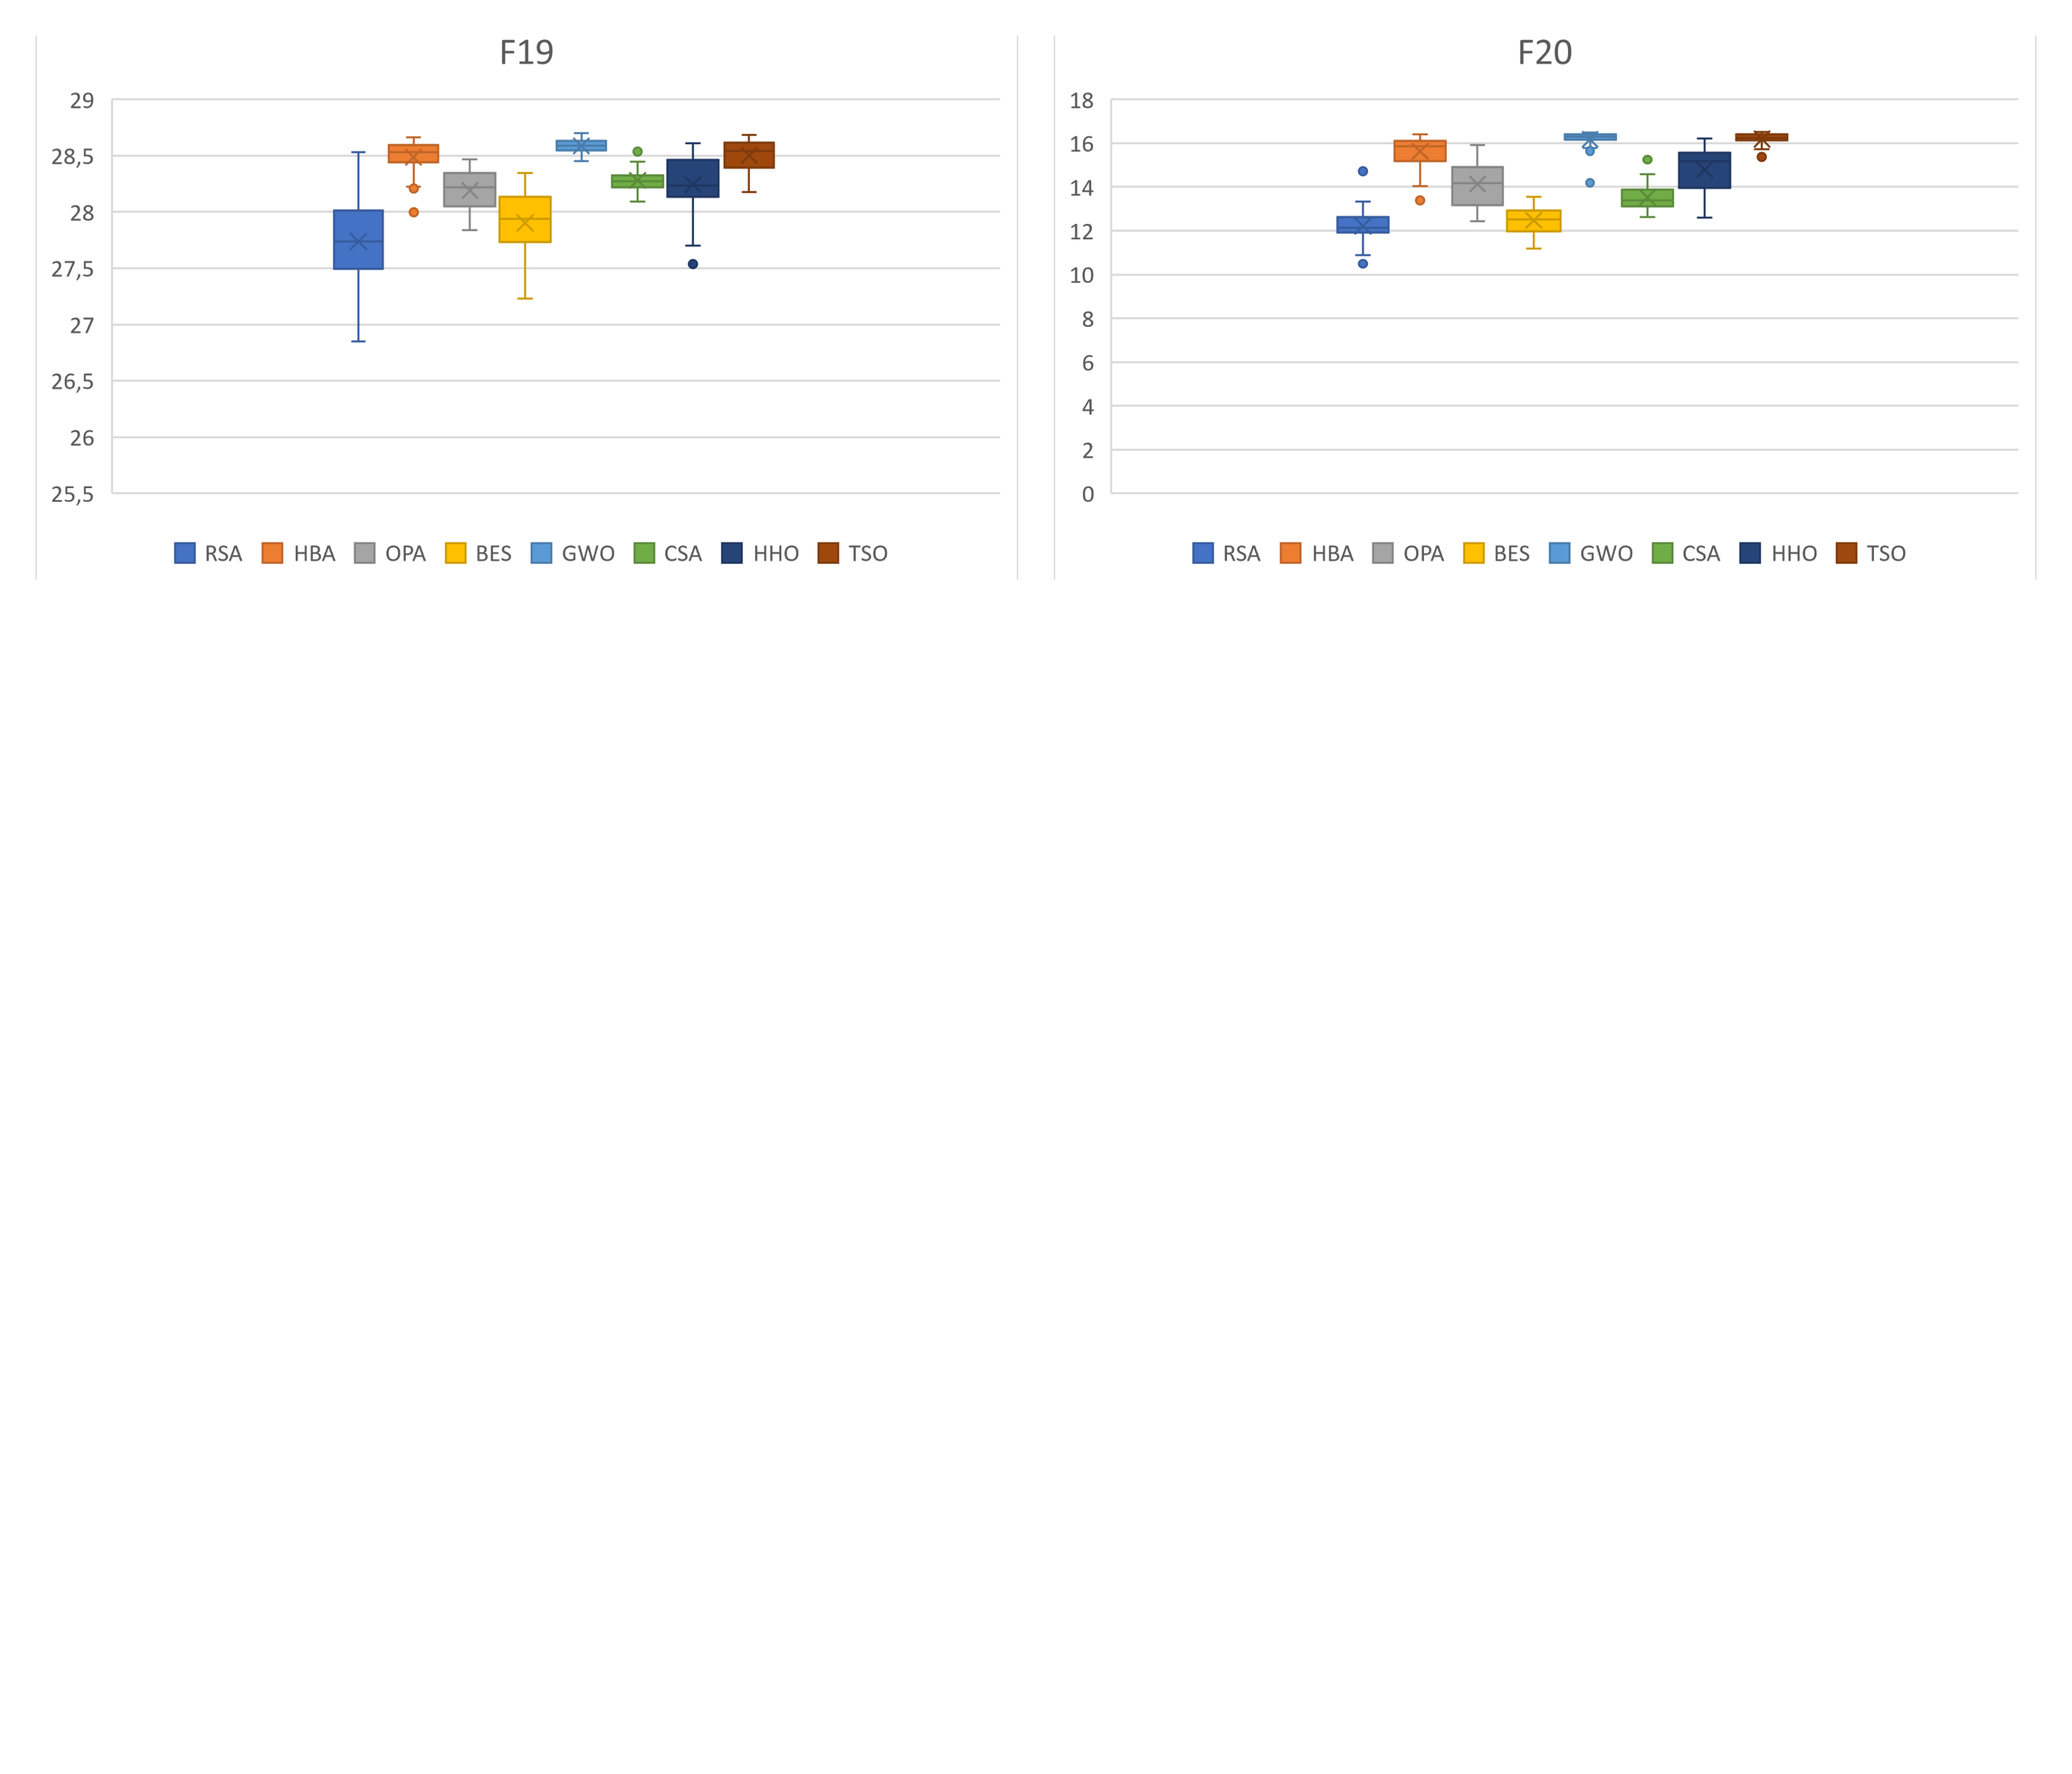
\includegraphics[width=\linewidth]{Fitness/Kapur/BoxPlot_Dim8/BoxPlots_19-20_Dim8.png}
		\vspace{-120pt} % Ajusta este valor según sea necesario
	\end{subfigure}
	\caption{Boxplot de los valores Fitness por cada imagen en la dimensión 8, desde la imagen 1 hasta la imagen 20,Función Objetivo entropía de Kapur}
	\label{fig:Boxplot_Fitnes_Dim8_Kapur}    
\end{figure}
\begin{itemize}
\item GWO: Se ha mostrado consistentemente como uno de los algoritmos con mejor rendimiento ~\ref{fig:Boxplot_Fitnes_Dim8_Kapur}. Exhibió medianas altas y rangos intercuartílicos (IQR) estrechos en la mayoría de los gráficos, lo que indica que no solo alcanza altos niveles de fitness sino que también es robusto y confiable en sus resultados.
\item CSA y HHO: Ambos algoritmos también mostraron un rendimiento fuerte y consistente a través de las diferentes evaluaciones. Sus medianas se mantuvieron altas y los IQR estrechos, reafirmando su eficacia y estabilidad como métodos de optimización.

\item RSA: Tendió a tener un rendimiento más bajo en comparación con los demás algoritmos. Aunque su IQR a veces era estrecho, lo que sugiere cierta consistencia, sus medianas eran generalmente más bajas y presentaba valores atípicos que indicaban resultados significativamente peores en algunos casos.

\item HBA, OPA, BES y TSO: Estos algoritmos mostraron un rendimiento medio, con medianas que generalmente se encontraban en el centro del rango y IQR que indicaban una variabilidad de moderada a alta. Ninguno de estos se destacó consistentemente como el mejor o el peor después del RSA, pero sus resultados no fueron tan robustos como los del GWO, CSA y HHO.
\end{itemize}
\subsubsection{Dimensión 9}

% Dimension 9
\begin{figure}
	\centering
	\begin{subfigure}{0.415\textwidth}
		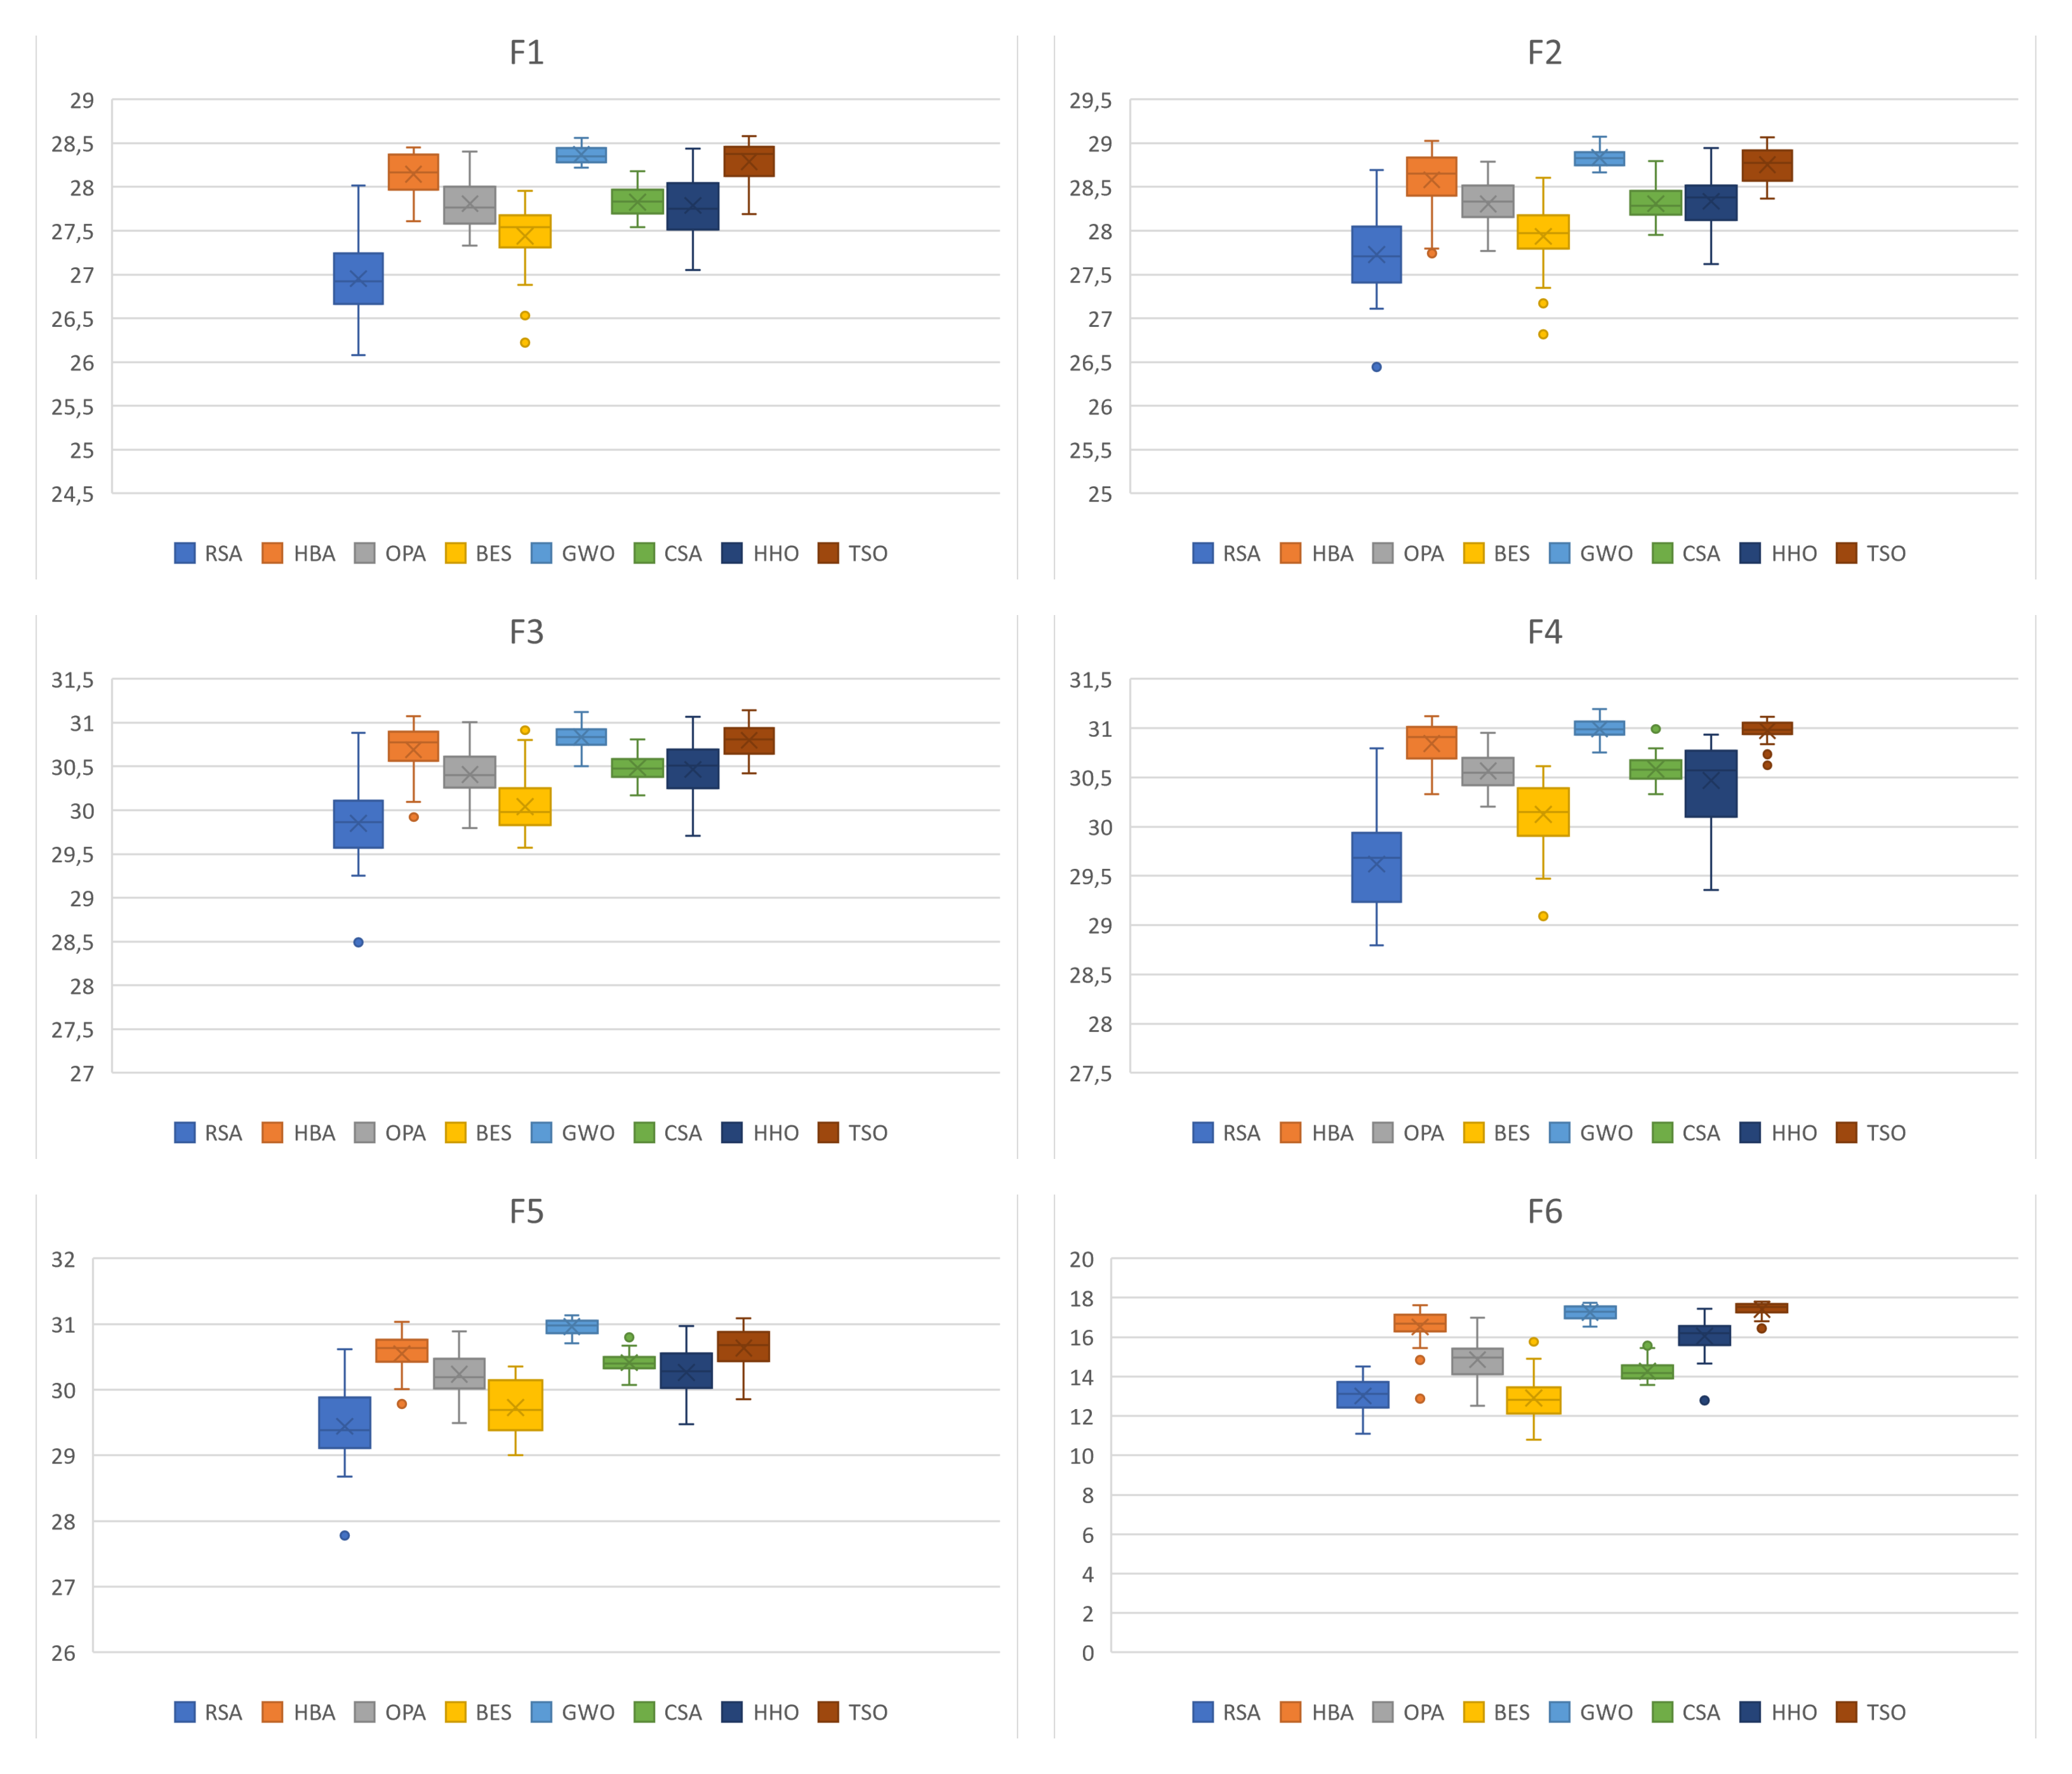
\includegraphics[width=\linewidth]{Fitness/Kapur/BoxPlot_Dim9/BoxPlots_1-6_Dim9.png}
	\end{subfigure}
	
	\begin{subfigure}{0.415\textwidth}
		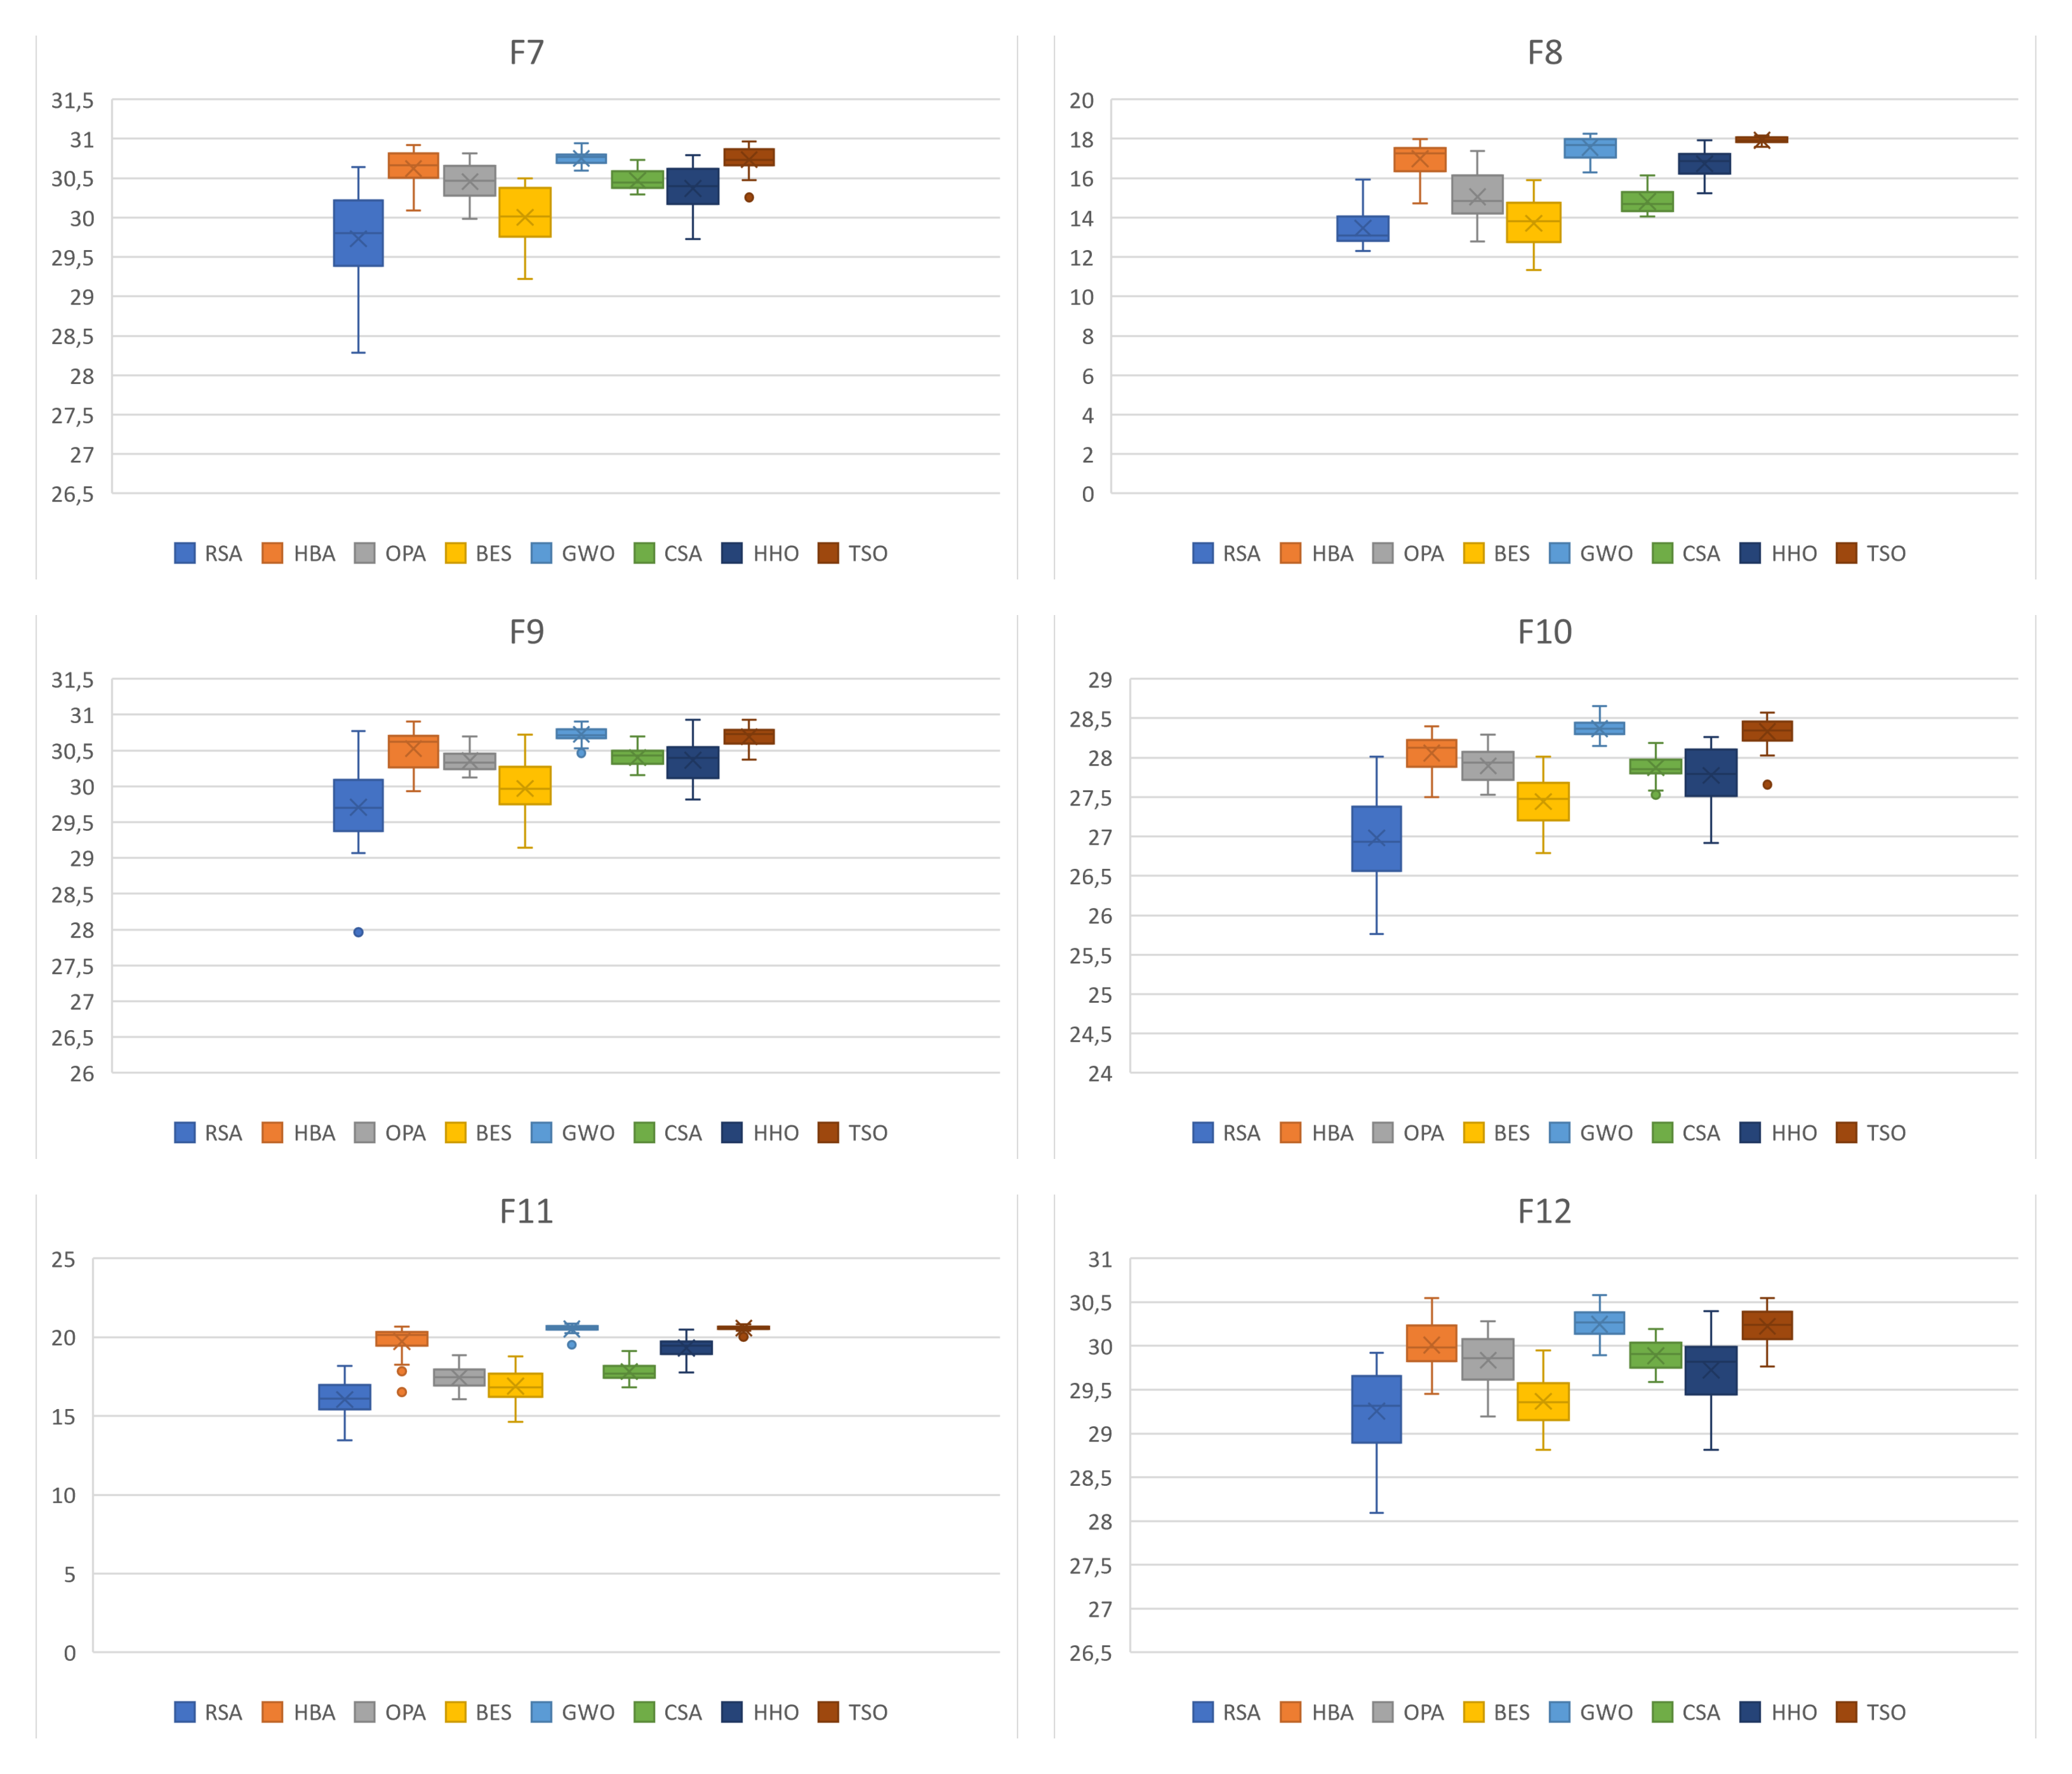
\includegraphics[width=\linewidth]{Fitness/Kapur/BoxPlot_Dim9/BoxPlots_7-12_Dim9.png}
	\end{subfigure}
	\begin{subfigure}{0.415\textwidth}
		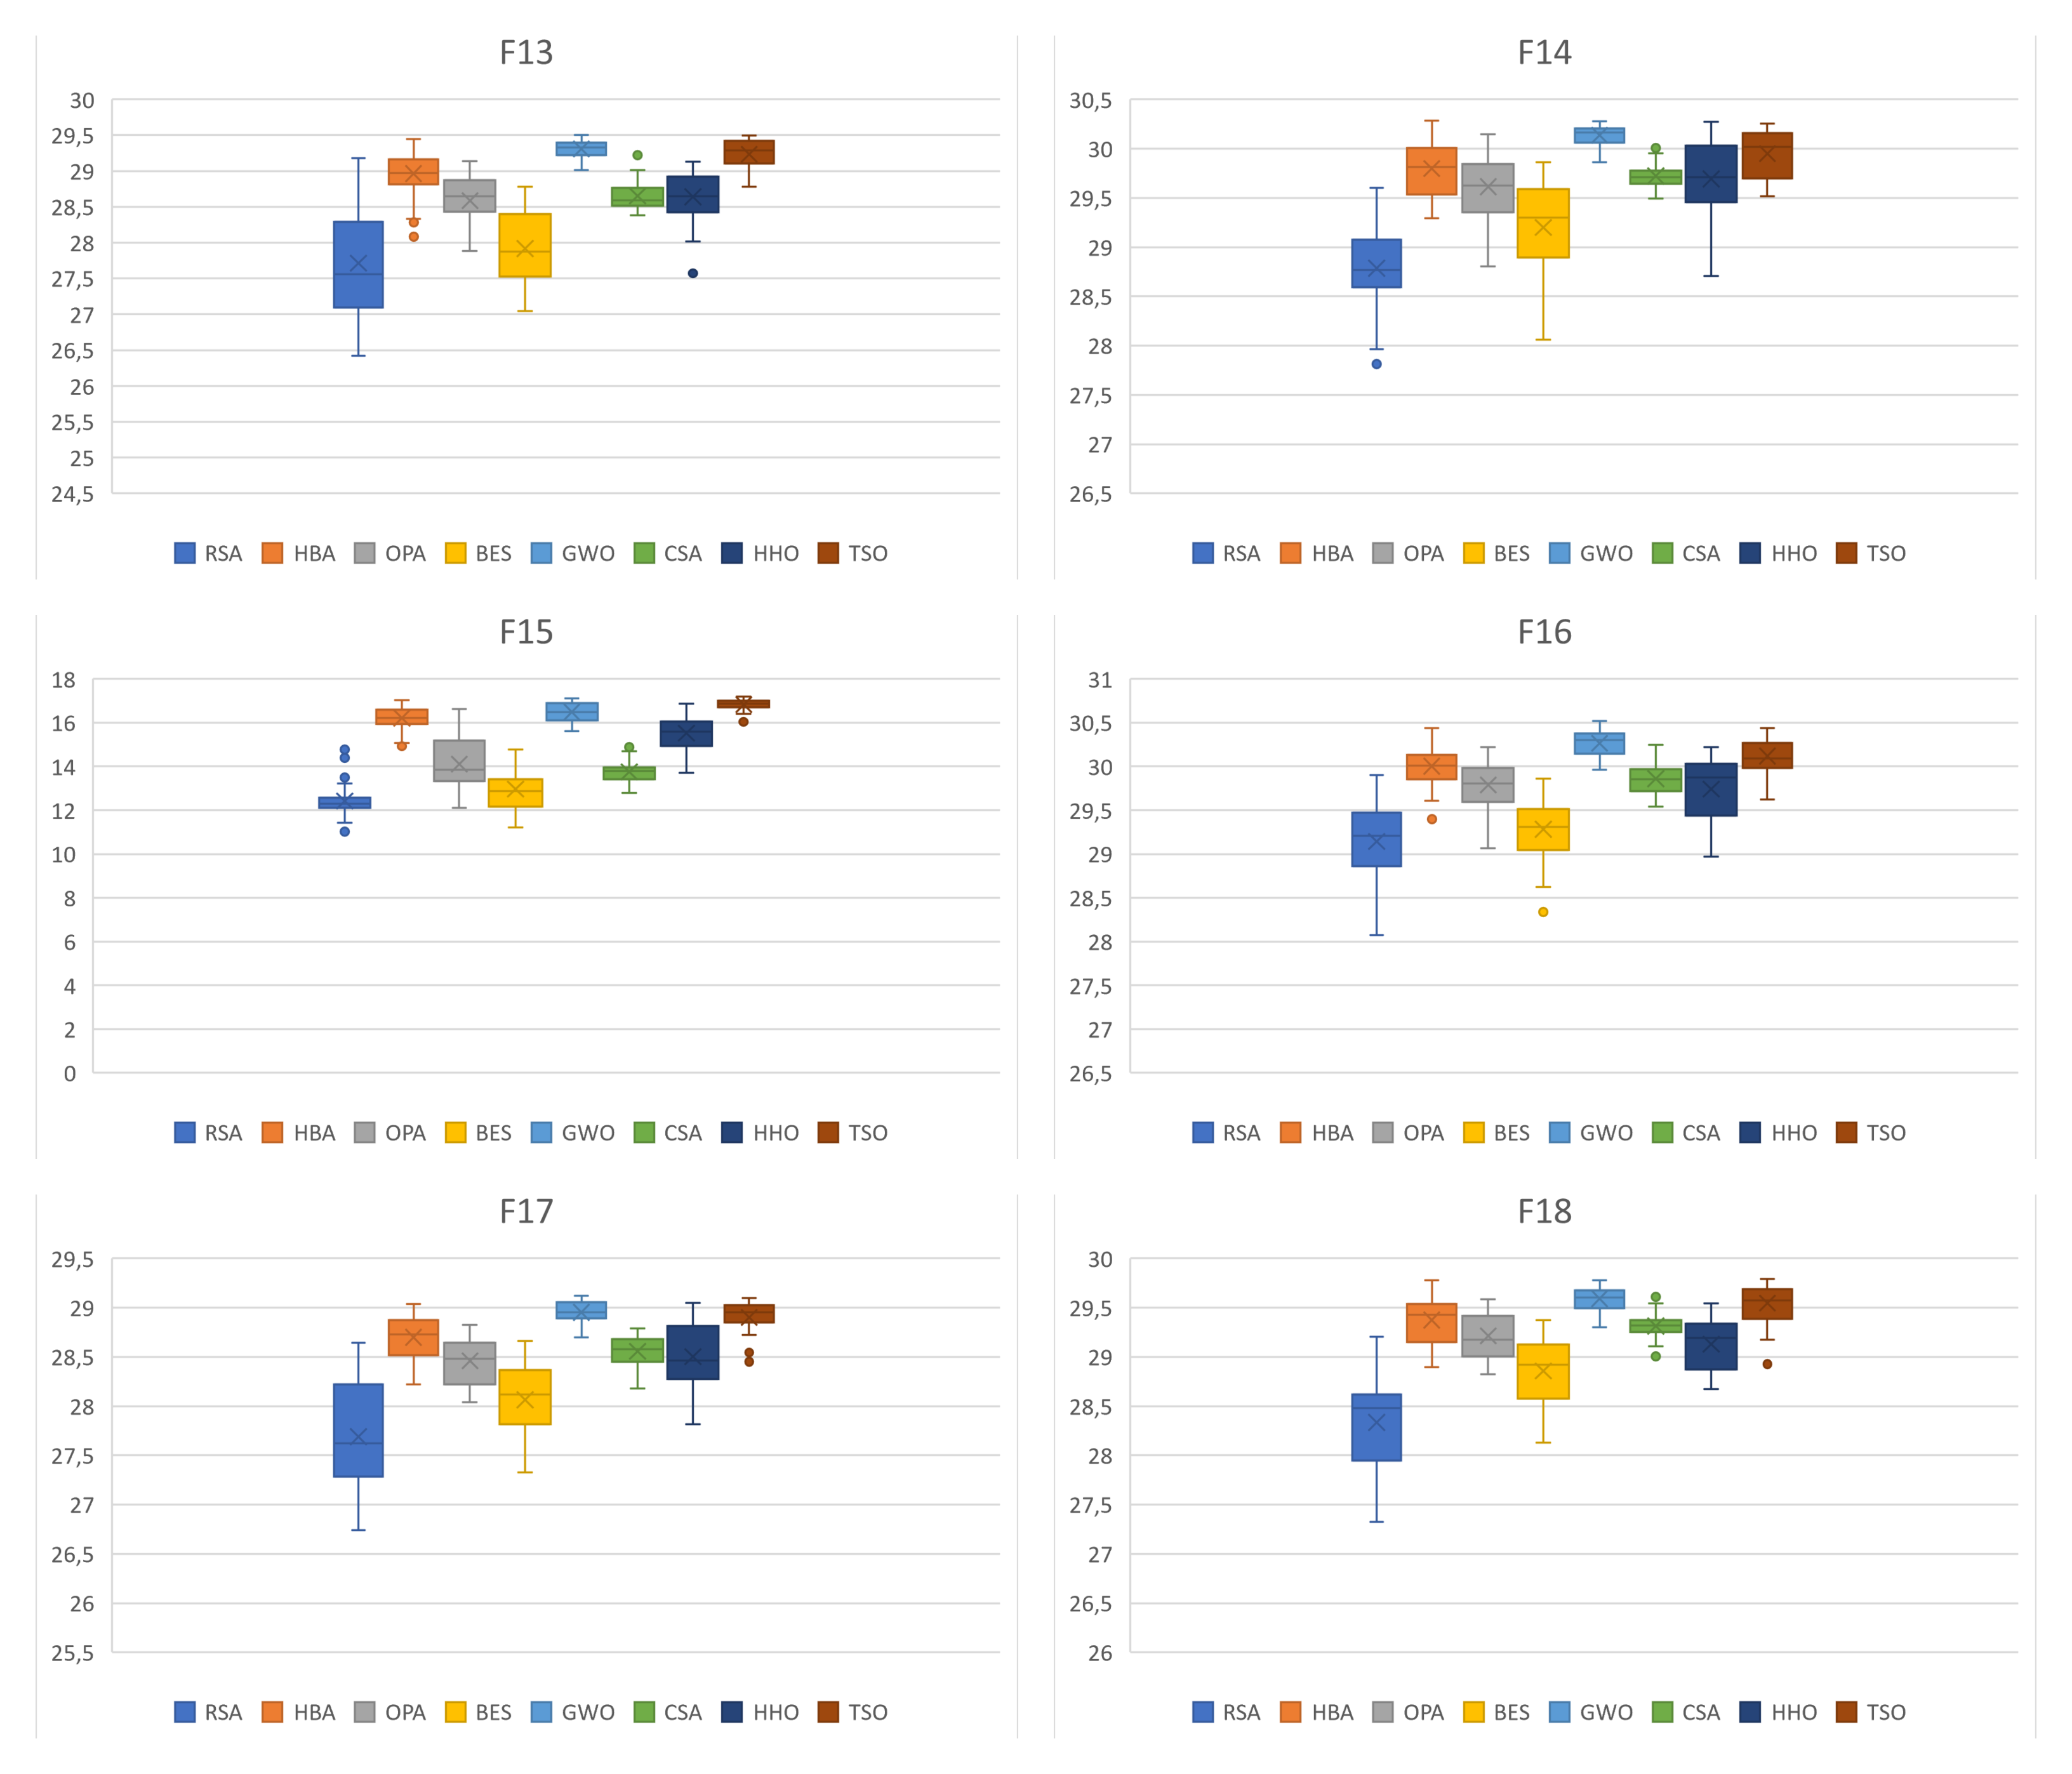
\includegraphics[width=\linewidth]{Fitness/Kapur/BoxPlot_Dim9/BoxPlots_13-18_Dim9.png}
	\end{subfigure}
	\begin{subfigure}{0.415\textwidth}
		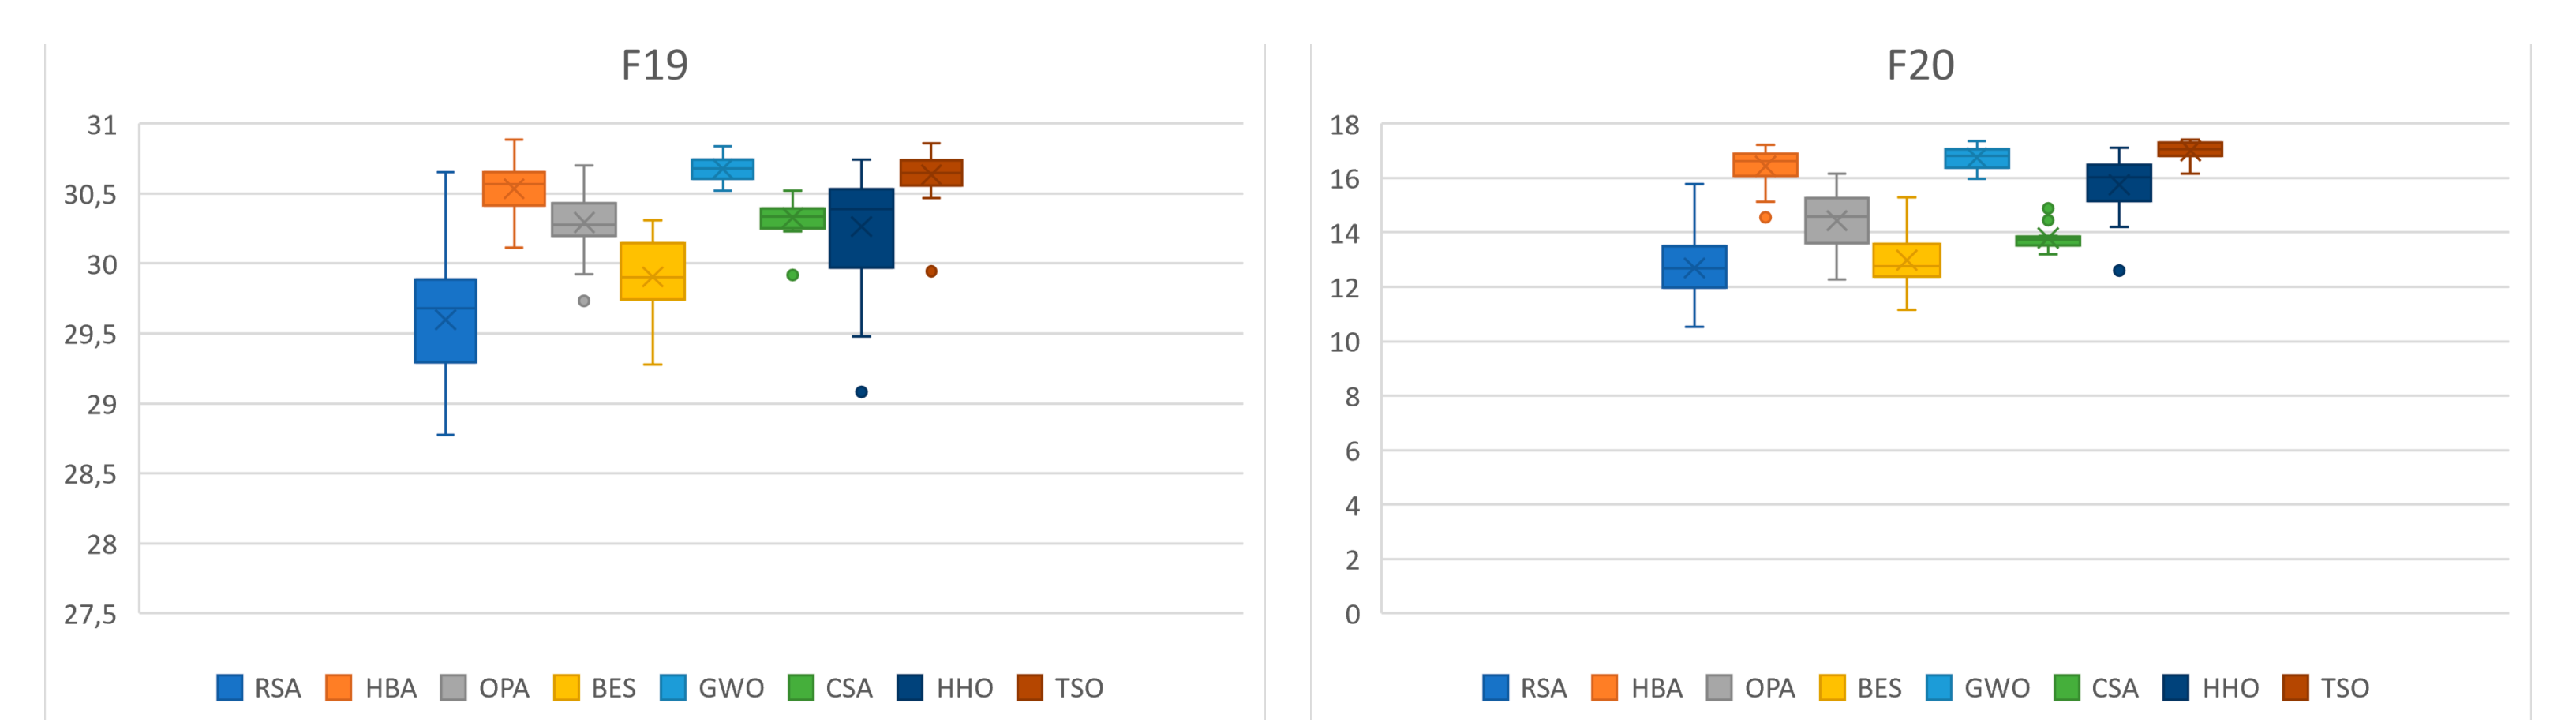
\includegraphics[width=\linewidth]{Fitness/Kapur/BoxPlot_Dim9/BoxPlots_19-20_Dim9.png}
		\vspace{4pt}
	\end{subfigure}
	\caption{Boxplot de los valores Fitness por cada imagen en la dimensión 9, desde la imagen 1 hasta la imagen 20,Función Objetivo entropía de Kapur}
	\label{fig:Boxplot_Fitnes_Dim9_Kapur}    
\end{figure}
 
\begin{itemize}

\item GWO: Este algoritmo ha demostrado consistentemente el mejor rendimiento. Tiene una mediana alta y una variabilidad baja, lo que indica que es eficaz y consistente en la segmentación de imágenes utilizando la entropía de Kapur.

\item HHO también ha mostrado un rendimiento sólido en las tres funciones objetivo. Aunque su variabilidad es un poco mayor que la de GWO, sigue siendo una opción confiable.

\item HBA, OPA, CSA: Estos algoritmos han mantenido un rendimiento intermedio en las tres funciones objetivo. Su mediana y variabilidad varían, pero en general, ofrecen resultados aceptables.

\item RSA ha mostrado un rendimiento generalmente más bajo en comparación con los otros algoritmos en las tres funciones objetivo. Tiene una mediana baja y una variabilidad alta, lo que sugiere resultados menos consistentes y menos óptimos.

\item TSO ha tenido un rendimiento variable a lo largo de las funciones objetivo. Aunque en F20 mostró una mejora en la mediana, su variabilidad y la presencia de valores atípicos plantean preocupaciones sobre su consistencia.

\item BES ha tenido un rendimiento variado, con una mediana más baja en comparación con algunos de los otros algoritmos. Su consistencia también podría ser mejorada.
\end{itemize}
\noindent En resumen ~\ref{fig:Boxplot_Fitnes_Dim9_Kapur}, GWO es consistentemente el mejor algoritmo en las tres funciones objetivo, seguido de cerca por HHO. Los algoritmos intermedios son HBA, OPA, CSA, y BES. RSA y TSO tienden a tener un rendimiento más bajo y variable.
%Computational experiments Otsu
\subsection{Resultados Función PSNR Entropia de Kapur}
\subsubsection{Dimensión 7}
\begin{itemize}
\item RSA: Este algoritmo ha mostrado un rendimiento promedio a lo largo de los diferentes boxplots, con una variabilidad moderada y pocos valores atípicos, lo que indica una consistencia razonable.
	
\item HBA: Generalmente presenta una mediana en el rango medio o ligeramente por debajo del promedio, con variabilidad moderada. En ocasiones, muestra valores atípicos que sugieren que puede tener episodios de rendimiento tanto superiores como inferiores al promedio.
	
\item OPA: Exhibe un rendimiento similar al RSA y HBA con una variabilidad comparable. Tiende a tener menos valores atípicos, lo que podría indicar un rendimiento más consistente en algunos casos.
	
\item BES: Este algoritmo consistentemente ha mostrado una mediana baja a través de los distintos boxplots, acompañada de una alta variabilidad. Esto sugiere un rendimiento generalmente más bajo y menos predecible.
	
\item GWO: Muestra un rendimiento medio con variabilidad moderada en la mayoría de los boxplots. En general, parece ser un algoritmo con un rendimiento estable, aunque no sobresaliente.
	
\item CSA: Tiene una mediana alta en la mayoría de los boxplots y una variabilidad moderada a baja, lo que indica un rendimiento generalmente bueno y consistente, convirtiéndolo en uno de los algoritmos más fiables de los evaluados.

\item HHO: Este algoritmo también muestra una mediana alta y una variabilidad moderada, similar al CSA, lo que sugiere un rendimiento robusto y confiable.
	
\item TSO: Aunque este algoritmo a menudo tiene la mediana más alta, también presenta una variabilidad considerable, lo que indica que mientras puede ofrecer el mejor rendimiento en términos de la métrica promedio, su consistencia es variable y puede tener episodios de rendimiento tanto muy altos como muy bajos.
	
\end{itemize}
\noindent En resumen, el CSA y el HHO parecen ser los algoritmos más confiables y consistentes en términos de las métricas evaluadas. El TSO, aunque potencialmente ofrece el mejor rendimiento, tiene una consistencia cuestionable. El BES parece ser el menos fiable debido a su bajo rendimiento y alta variabilidad. Los algoritmos RSA, HBA, y OPA ofrecen un rendimiento intermedio y una consistencia razonable, mientras que el GWO se mantiene en un rendimiento medio sin destacar particularmente en ninguna métrica.
% Boxplot de la 1 a la imagen 20 funcion PSNR
% Dimension 7
\begin{figure}[htbp]
	\centering
	\begin{subfigure}{0.4\textwidth}
		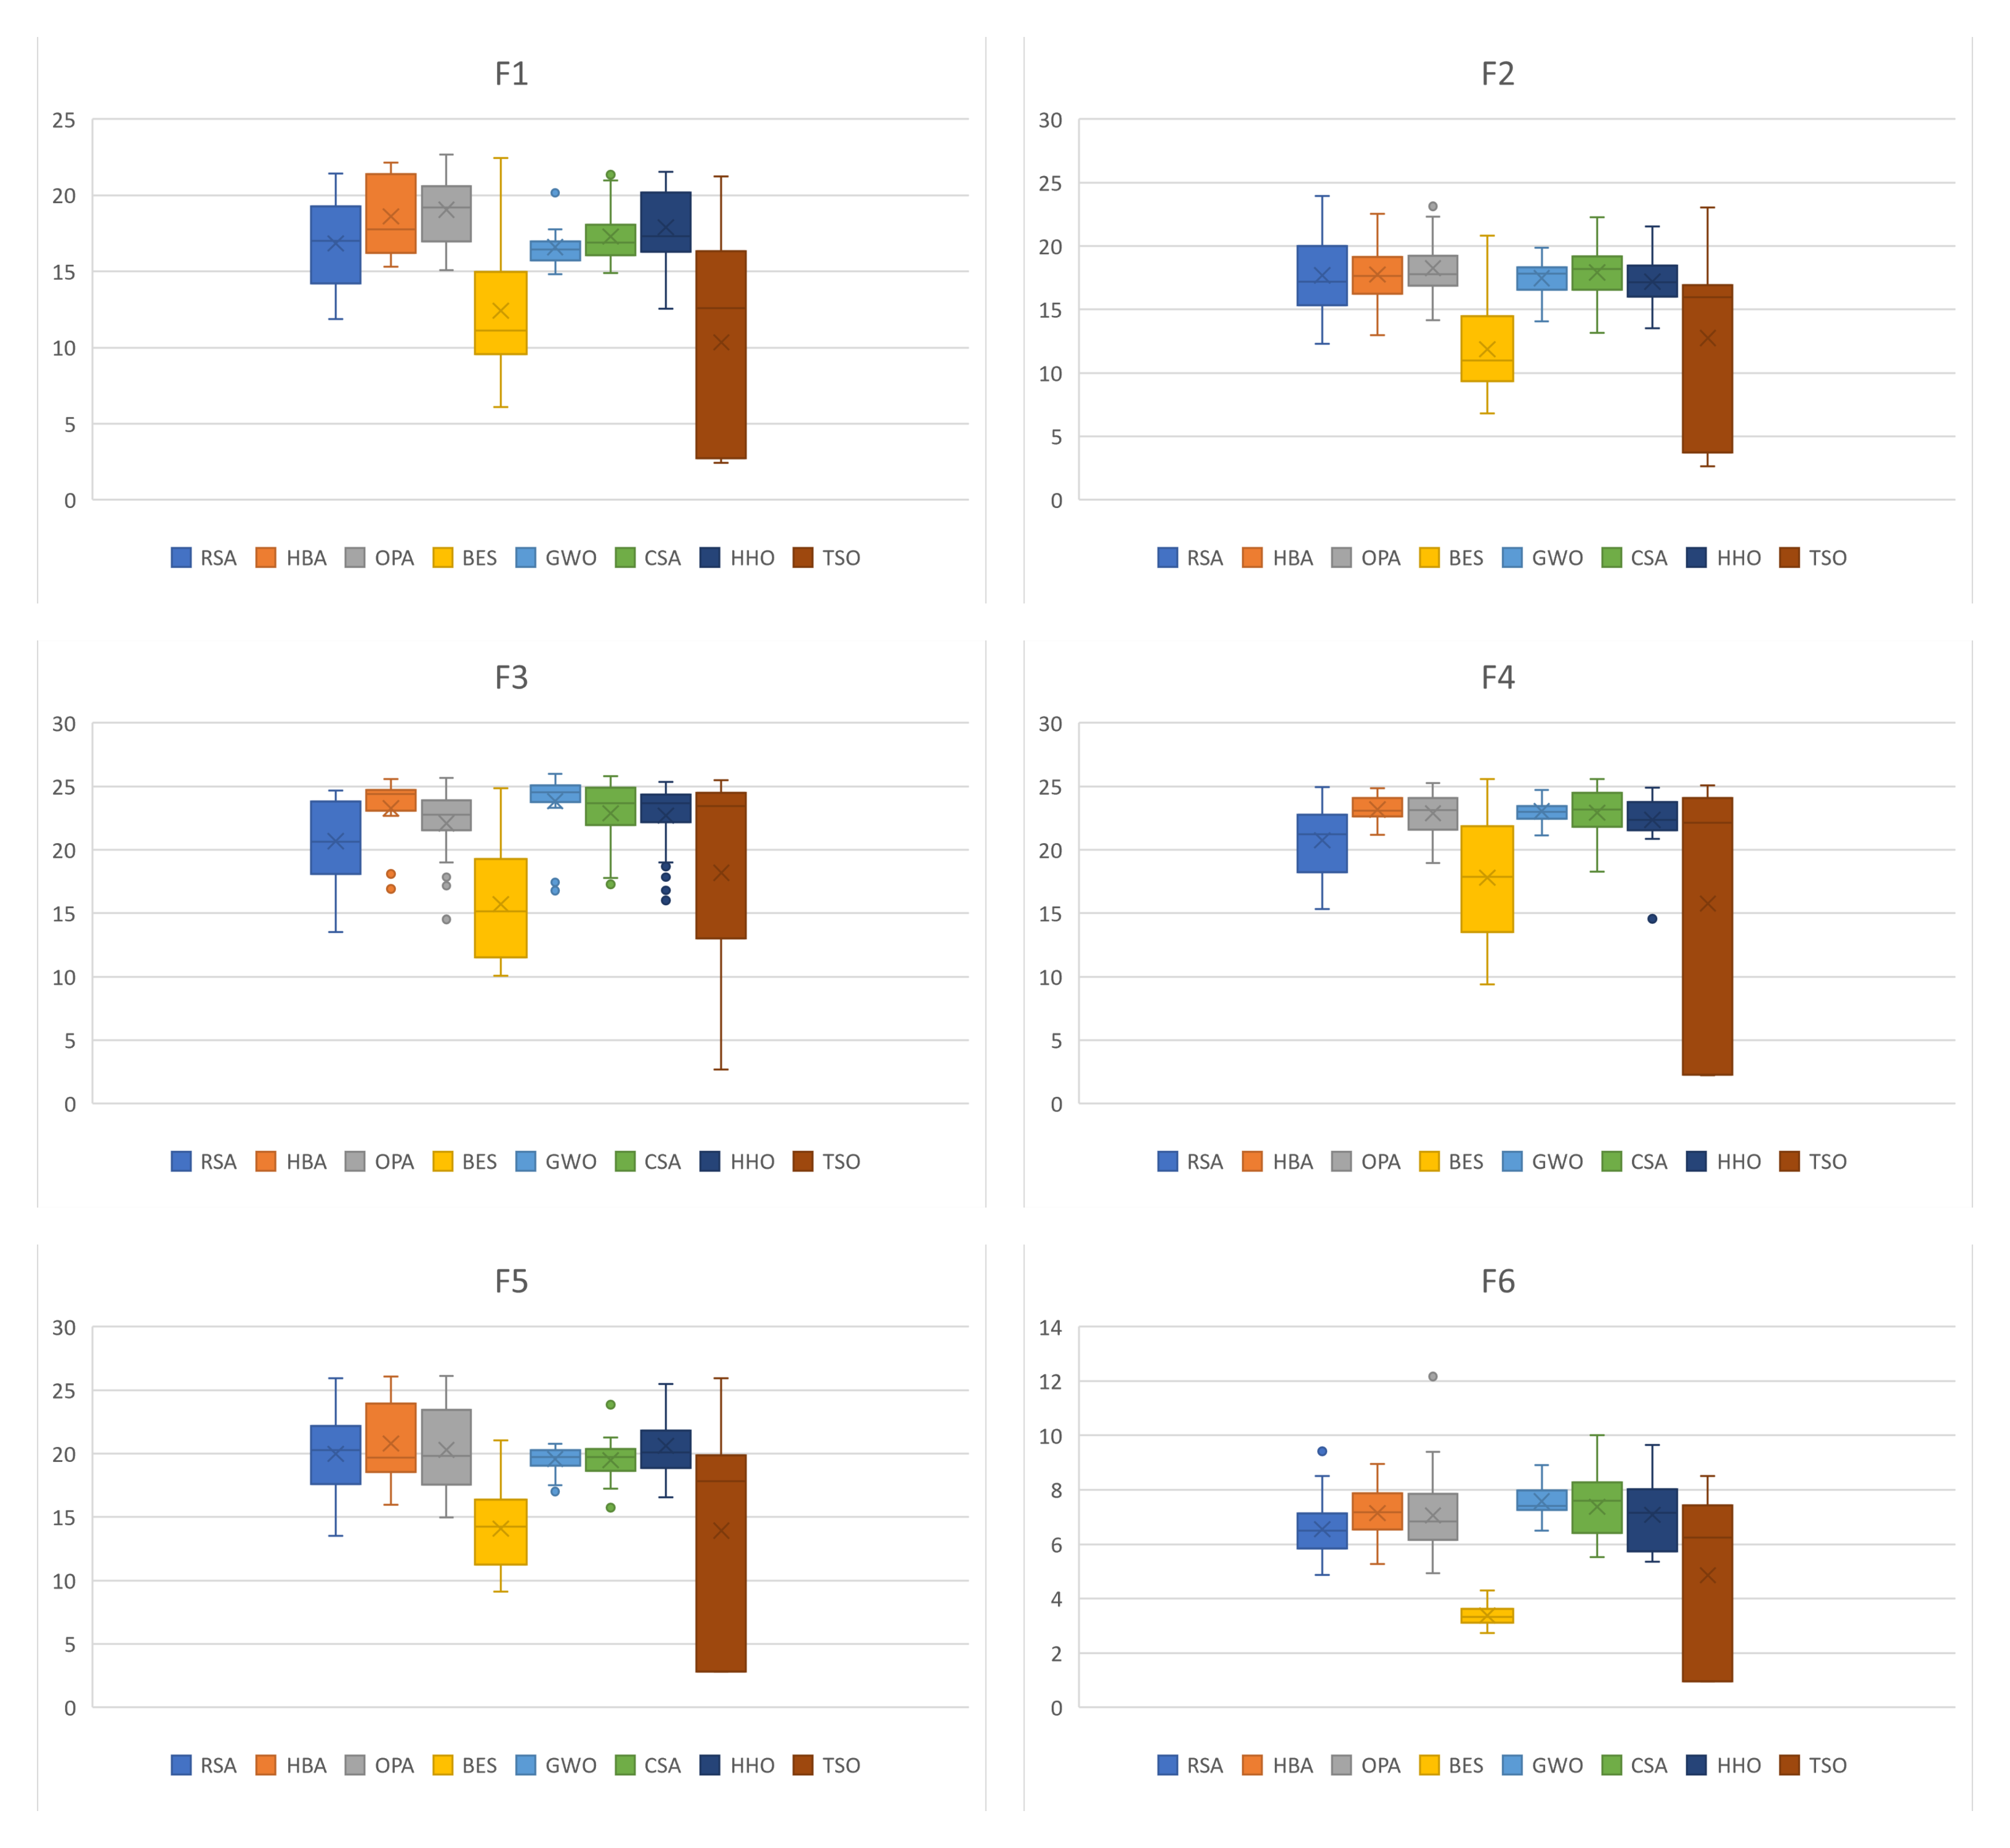
\includegraphics[width=\linewidth]{PSNR/Kapur/Dim7/PSNR_Dim7_Kapur_1_6.png}
	\end{subfigure}
	
	\begin{subfigure}{0.4\textwidth}
		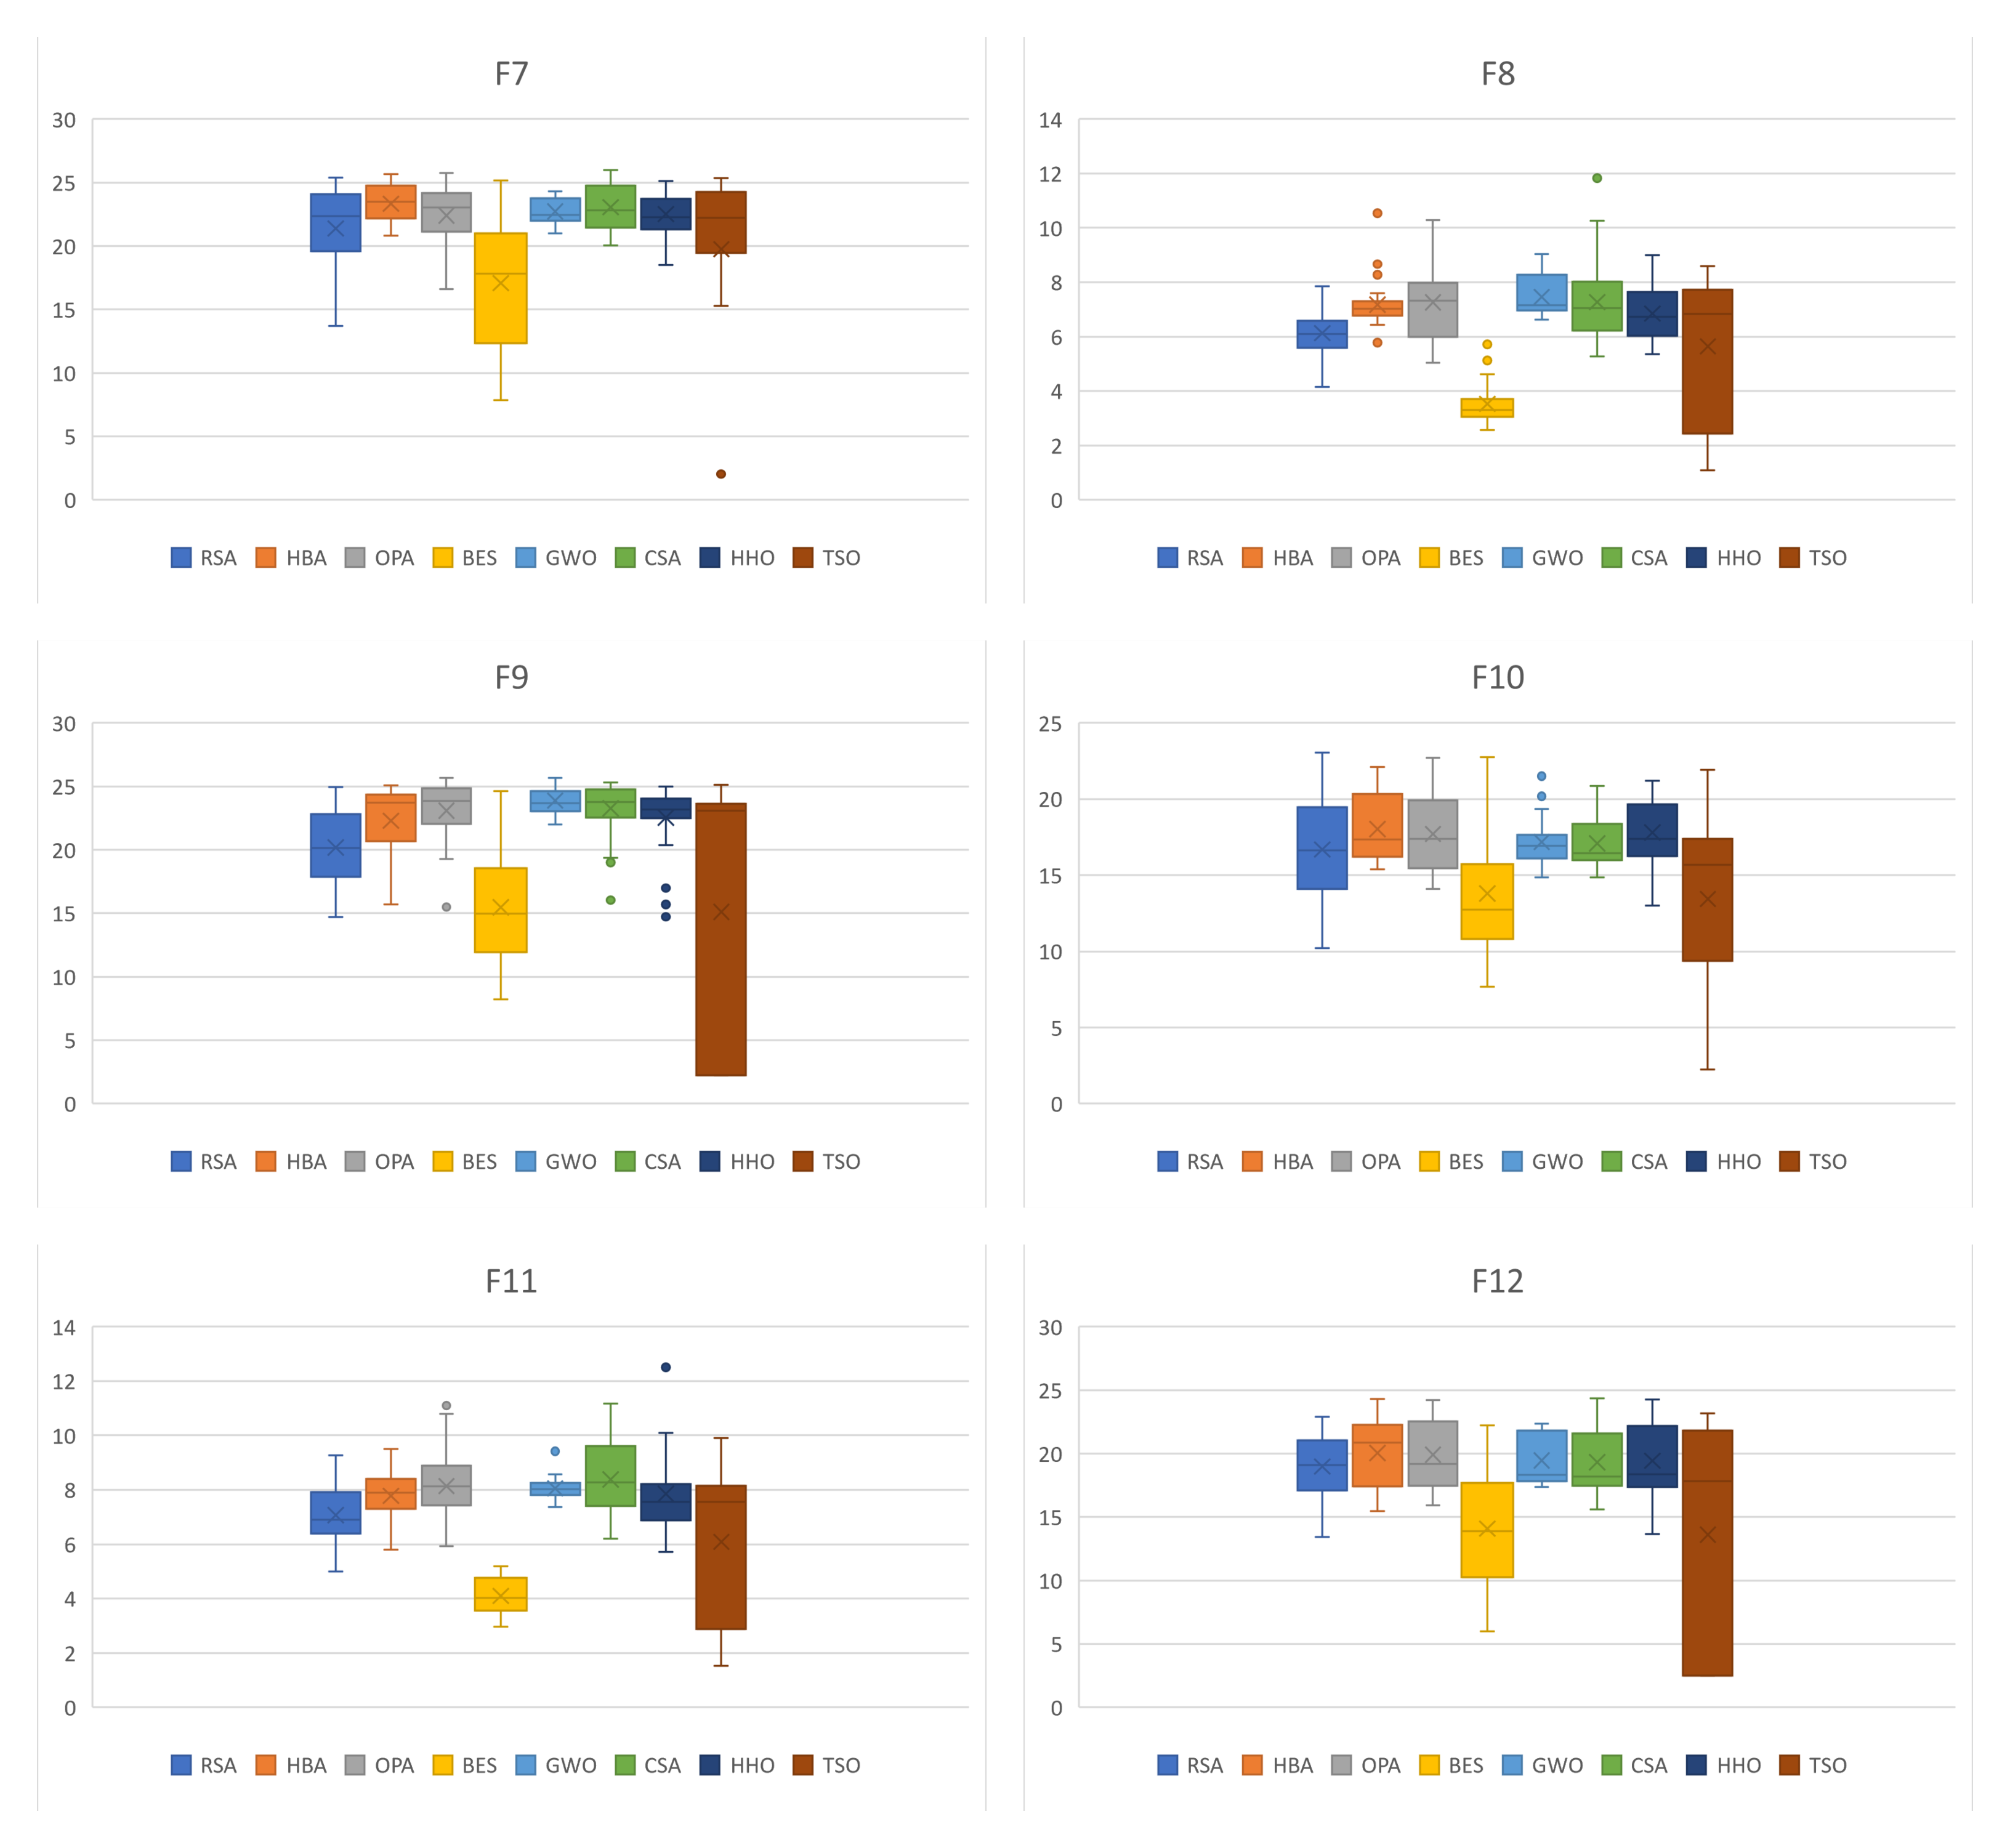
\includegraphics[width=\linewidth]{PSNR/Kapur/Dim7/PSNR_Dim7_Kapur_7_12.png}
	\end{subfigure}
	\begin{subfigure}{0.4\textwidth}
		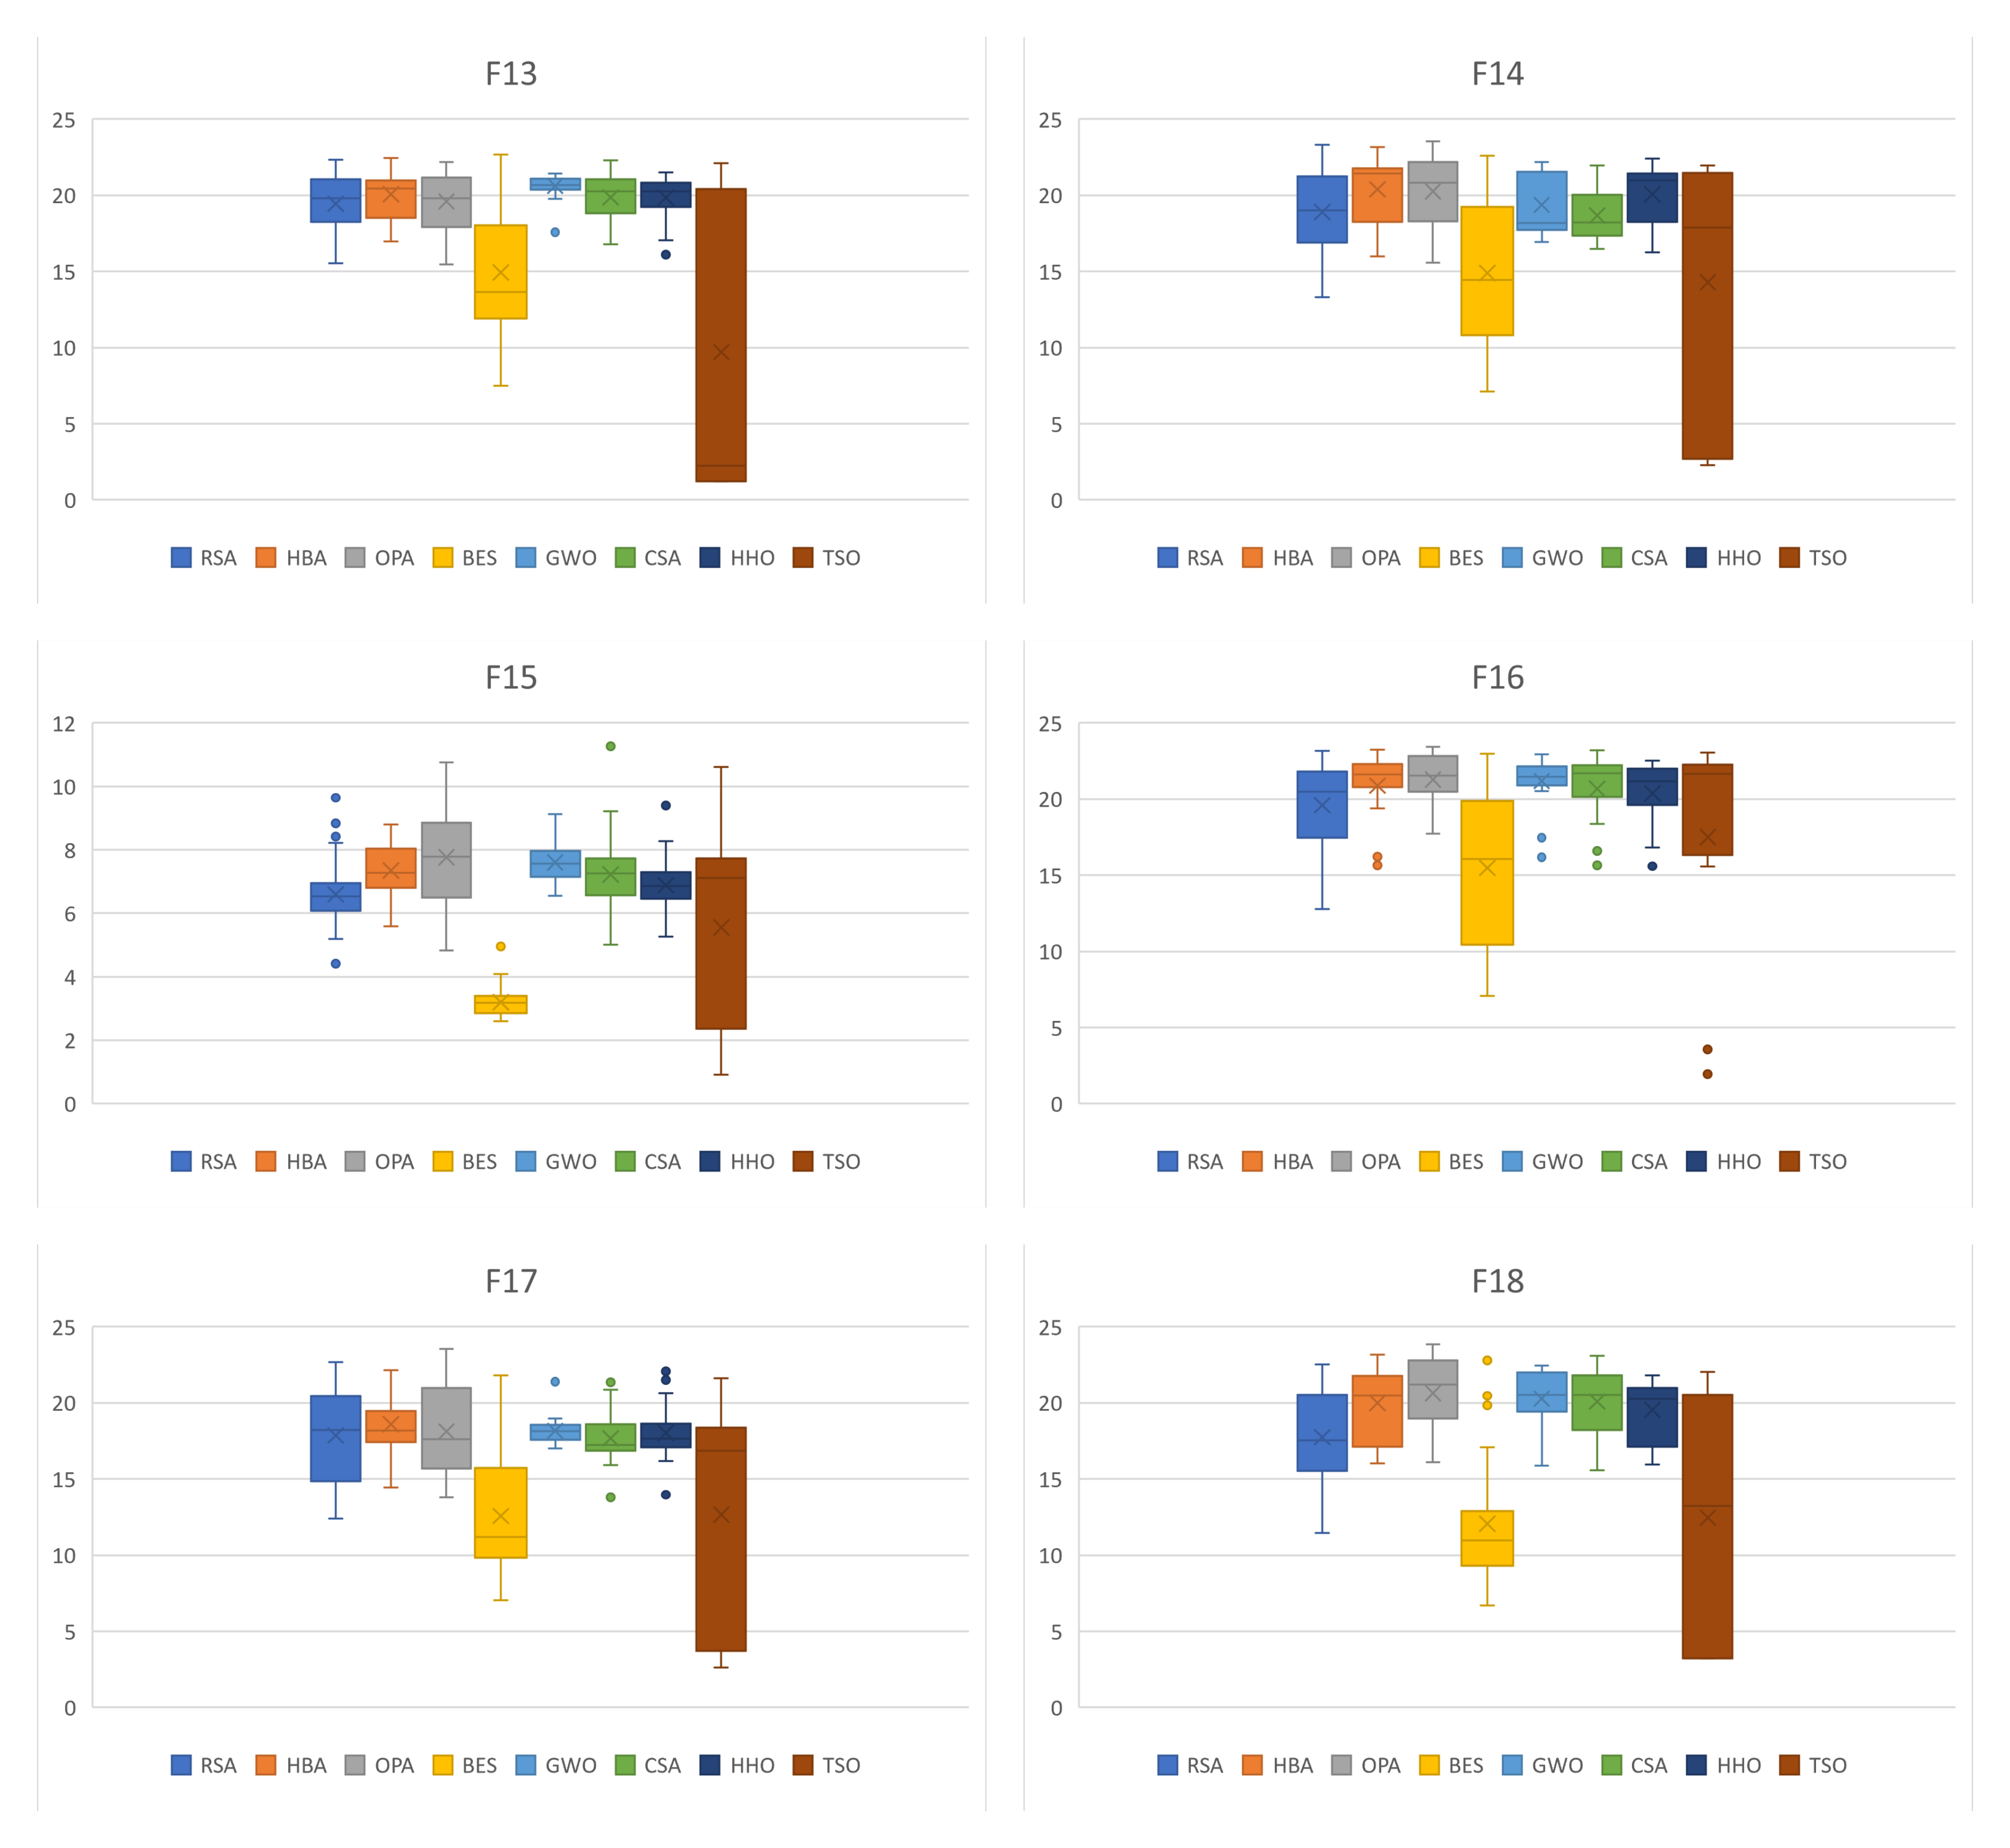
\includegraphics[width=\linewidth]{PSNR/Kapur/Dim7/PSNR_Dim7_Kapur_13_18.png}
		%\vspace{-150pt} % Ajusta este valor según sea necesario
	\end{subfigure}  
	\begin{subfigure}{0.4\textwidth}
		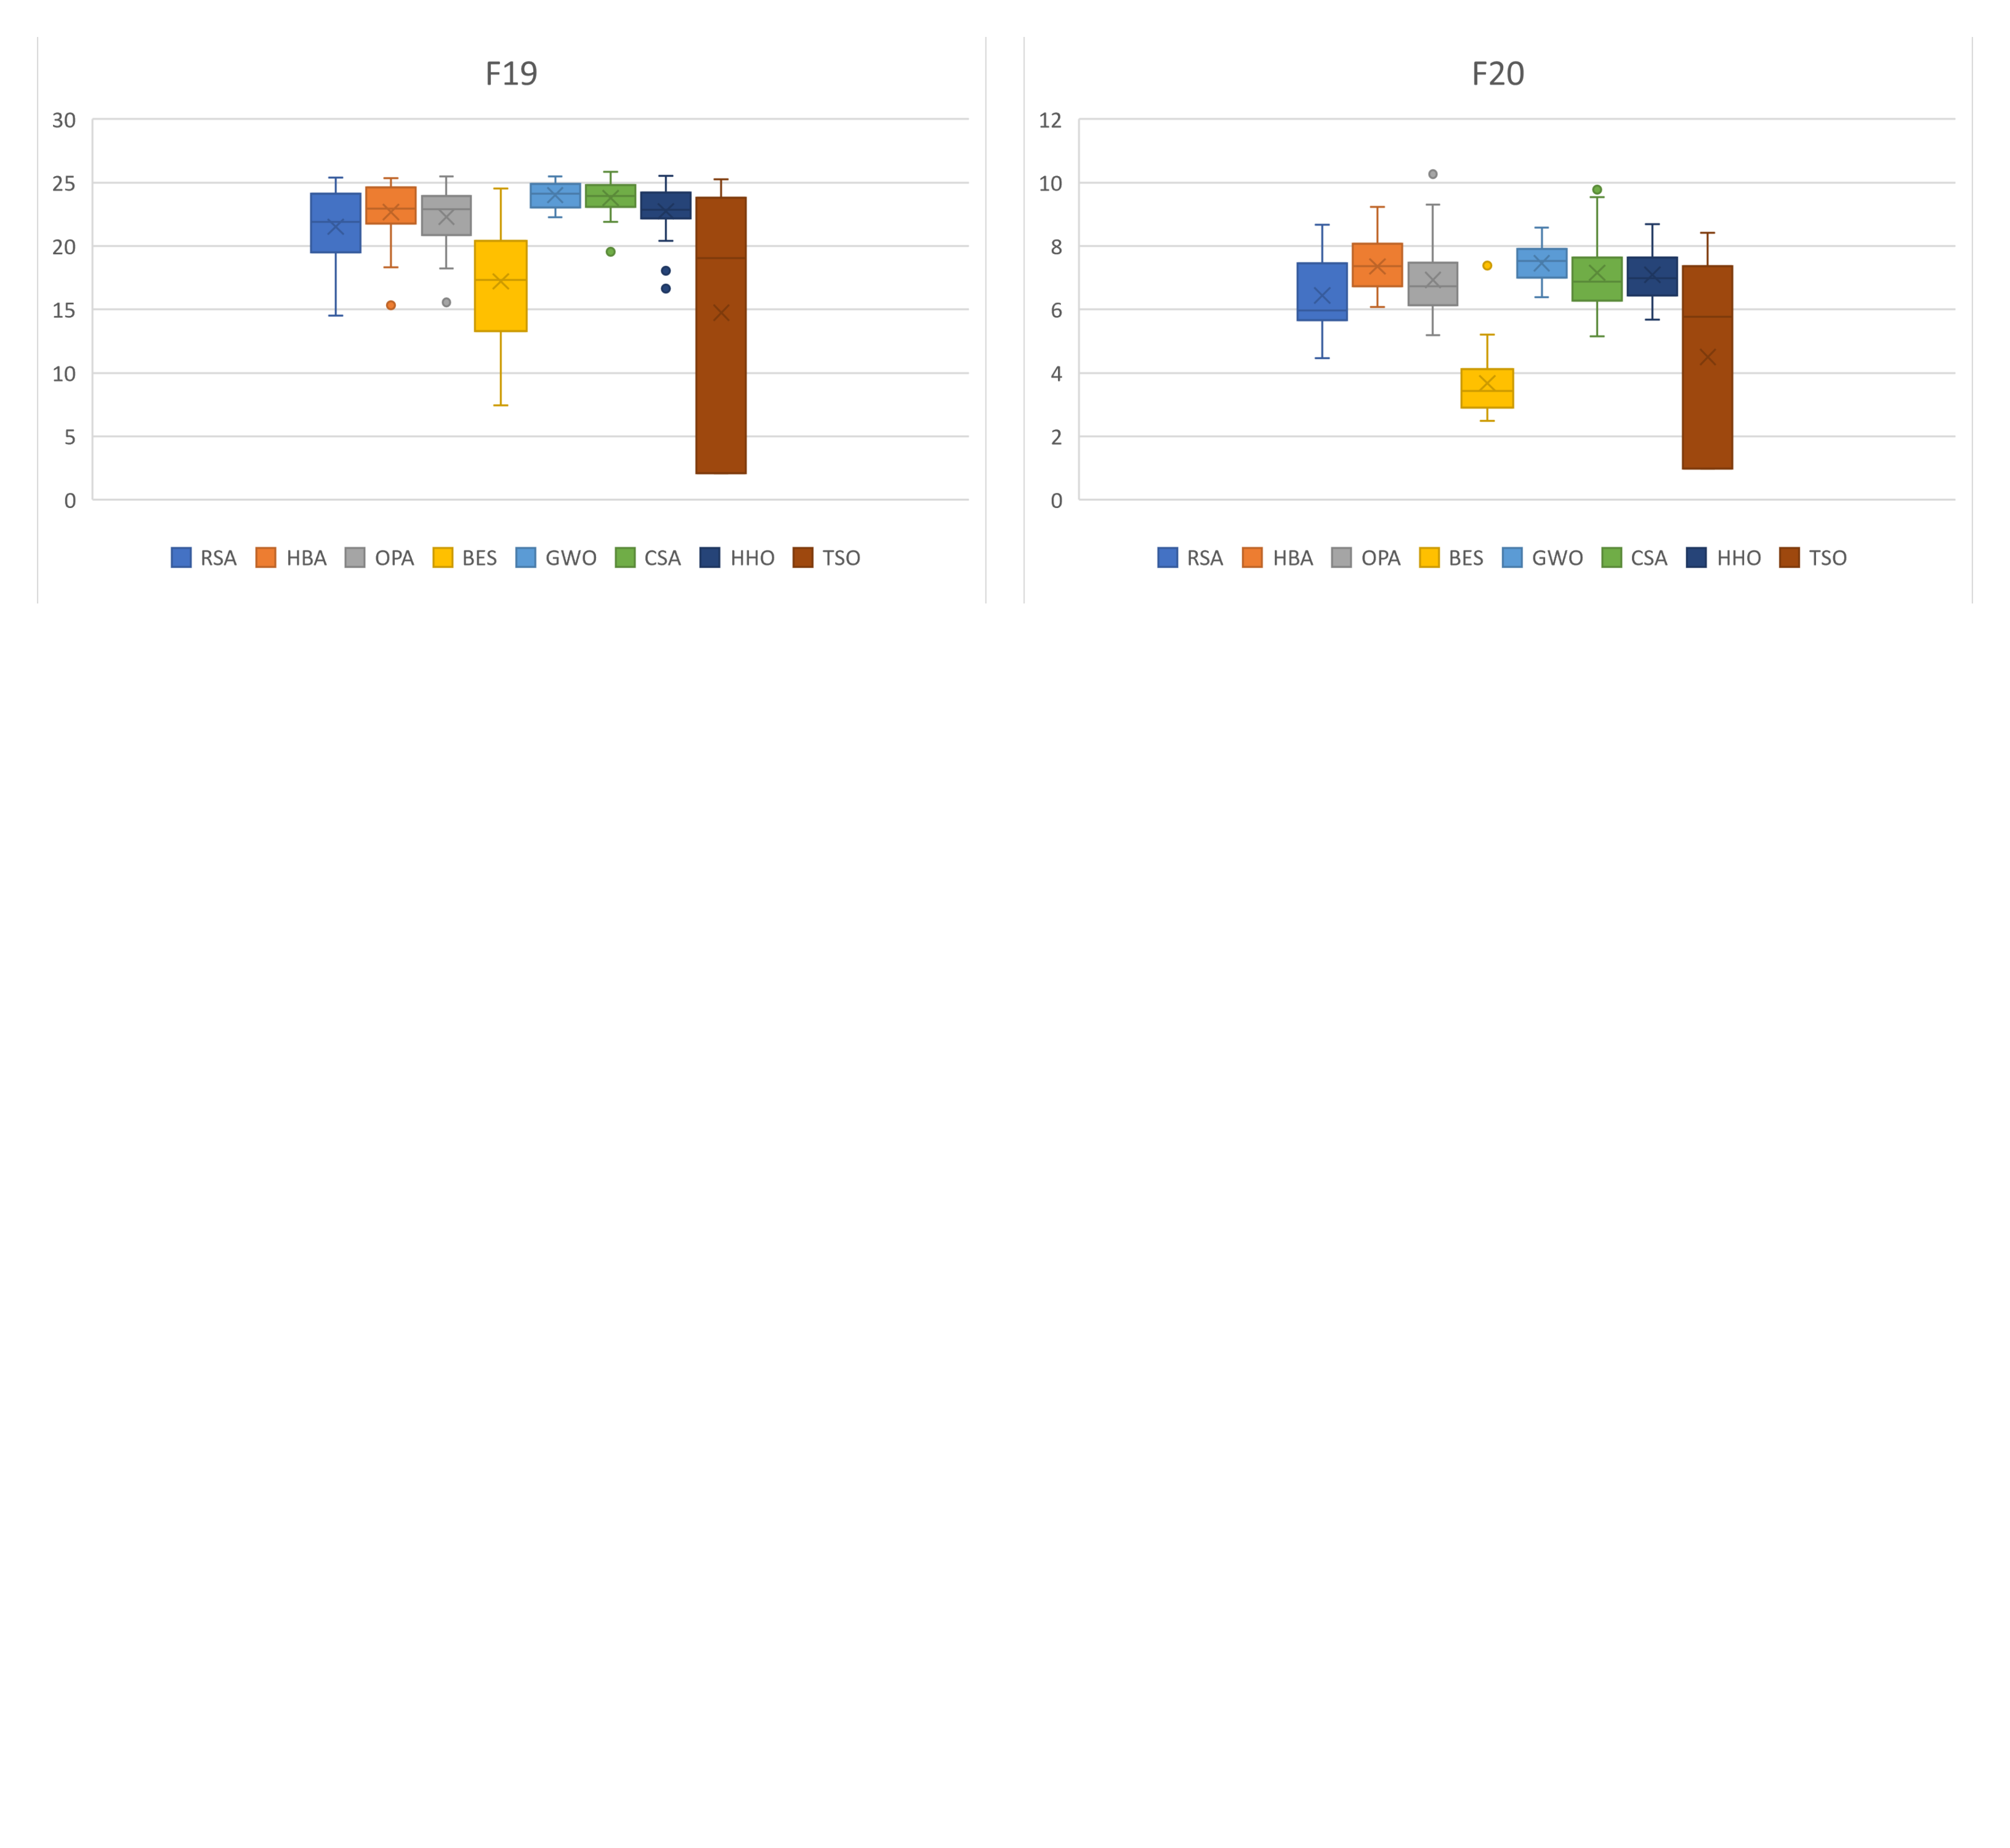
\includegraphics[width=\linewidth]{PSNR/Kapur/Dim7/PSNR_Dim7_Kapur_19_20.png}
		\vspace{-120pt} % Ajusta este valor según sea necesario
	\end{subfigure}
	\caption{Boxplot de los valores PSNR por cada imagen en la dimensión 7, desde la imagen 1 hasta la imagen 20,Función Entropia de Kapur}
	\label{fig:imagenes}    
\end{figure}

\subsubsection{Dimensión 8}
\begin{itemize}
\item RSA: Este algoritmo ha mostrado una mediana de PSNR generalmente en el rango medio a alto en todas las imágenes, con una variabilidad moderada. Esto indica un rendimiento consistente con una calidad de imagen fiable en diferentes instancias.

\item HBA: El HBA ha tenido un rendimiento similar al RSA con medianas de PSNR en el rango medio. La variabilidad ha sido moderada, y la presencia de algunos valores atípicos sugiere que puede alcanzar altos niveles de calidad en ciertas condiciones.

\item OPA: El OPA ha exhibido medianas de PSNR en el rango medio con variabilidad moderada en todas las imágenes. Esto apunta a un rendimiento promedio sin grandes fluctuaciones, lo cual es deseable para aplicaciones que necesitan consistencia.

\item BES: El BES consistentemente ha mostrado las medianas más bajas de PSNR y alta variabilidad, indicando un rendimiento inferior en términos de calidad de imagen en comparación con los demás algoritmos.

\item GWO: Este algoritmo ha tenido medianas de PSNR generalmente en el rango medio y variabilidad moderada, lo que indica un rendimiento promedio en términos de calidad de imagen.

\item CSA: El CSA ha tenido medianas de PSNR altas en la mayoría de los boxplots, con variabilidad moderada. Esto señala un rendimiento consistente y robusto, lo que lo hace confiable para obtener una alta calidad de imagen.

\item HHO: Similar al CSA, el HHO ha mostrado medianas de PSNR altas y variabilidad moderada en todas las imágenes, lo que indica un rendimiento de alta calidad y fiabilidad.

\item TSO: Aunque el TSO ha tenido las medianas más altas de PSNR, indicando el potencial para la mejor calidad de imagen, también ha mostrado una variabilidad significativa. Esto implica que su rendimiento puede ser el mejor en promedio, pero con una consistencia que puede ser problemática para algunas aplicaciones.
\end{itemize}
En resumen, CSA y HHO han demostrado ser los algoritmos más fiables y consistentes en términos de calidad de imagen a través de las diferentes imágenes examinadas. TSO ha mostrado un potencial de alta calidad, pero con inconsistencias. BES ha sido el menos fiable y con el rendimiento más bajo. Los algoritmos RSA, HBA, y OPA han ofrecido un rendimiento medio y consistente, sin destacar especialmente en ninguna métrica.
%% Boxplot de los valores PSNR por cada imagen en la dimensión 8, desde la imagen 1 hasta la imagen 20, Función Entropía de Kapur
\begin{figure}[htbp] % 'htbp' indica las preferencias de ubicación: aquí, arriba, abajo, en una página especial de figuras.
	\centering % Esto centrará las imágenes
	\begin{subfigure}{0.4\textwidth}
		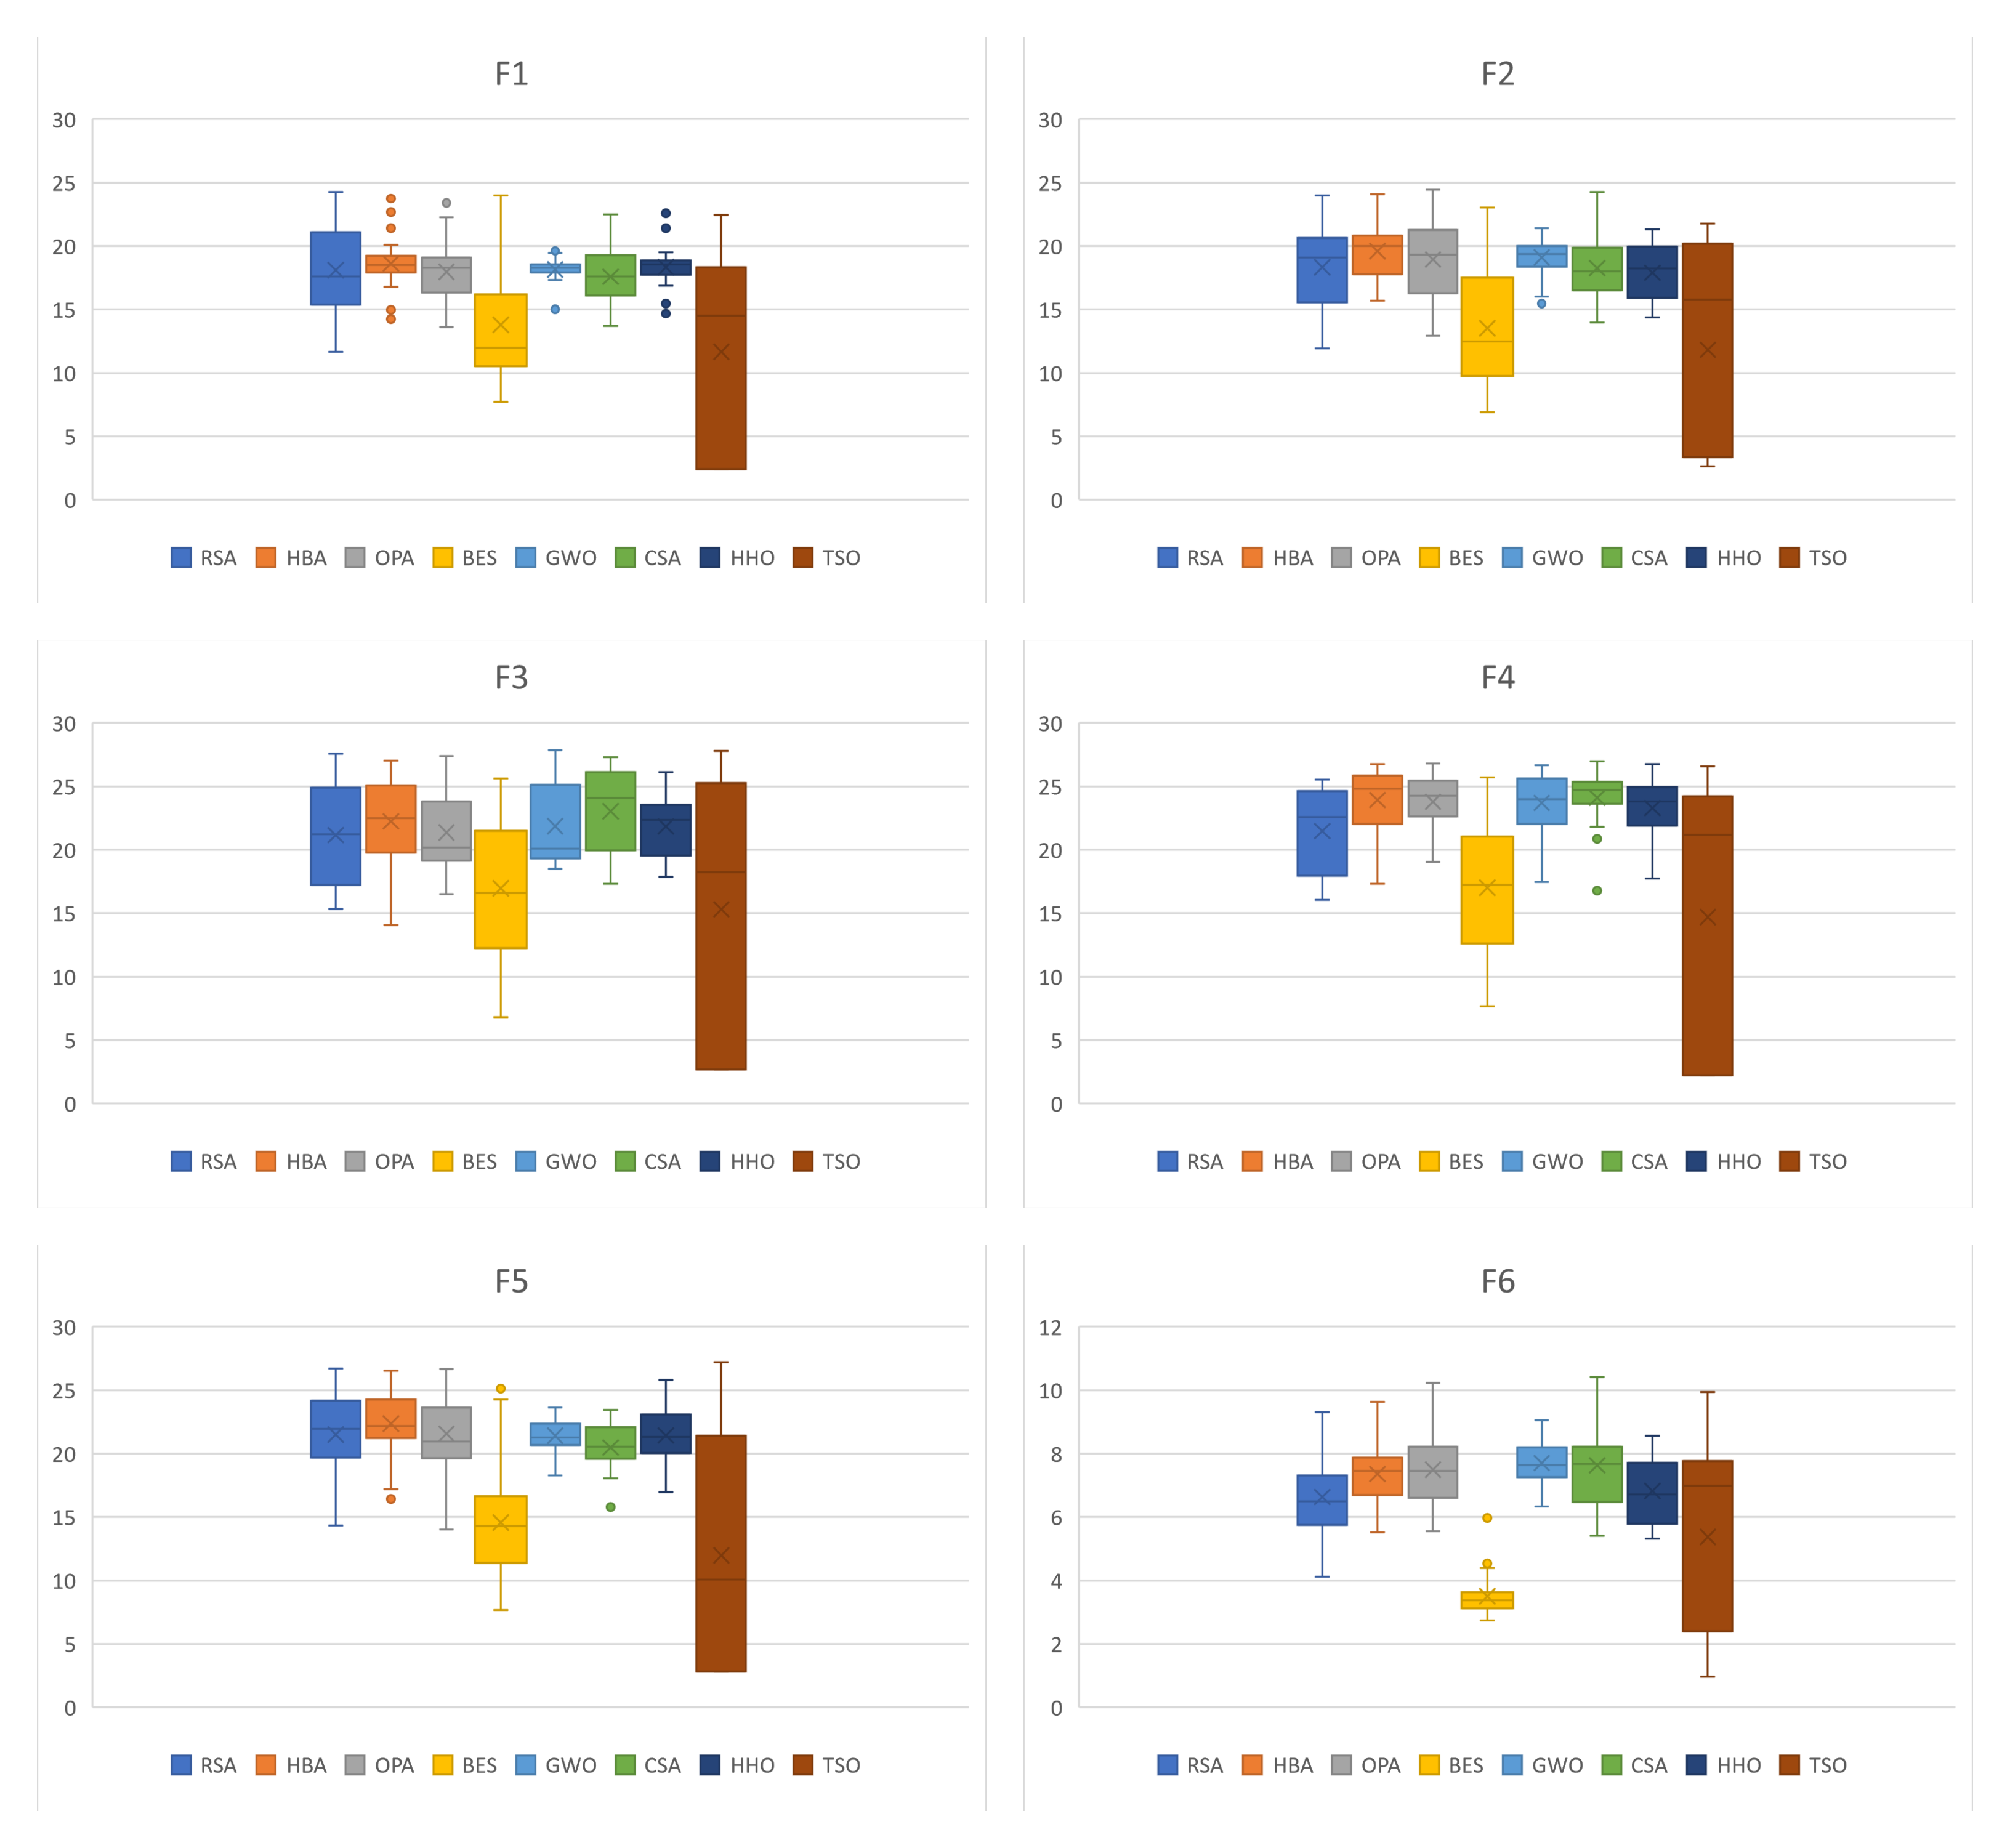
\includegraphics[width=\linewidth]{PSNR/Kapur/Dim8/PSNR_Dim8_Kapur_1_6.png}
	\end{subfigure}
	
	\begin{subfigure}{0.4\textwidth}
		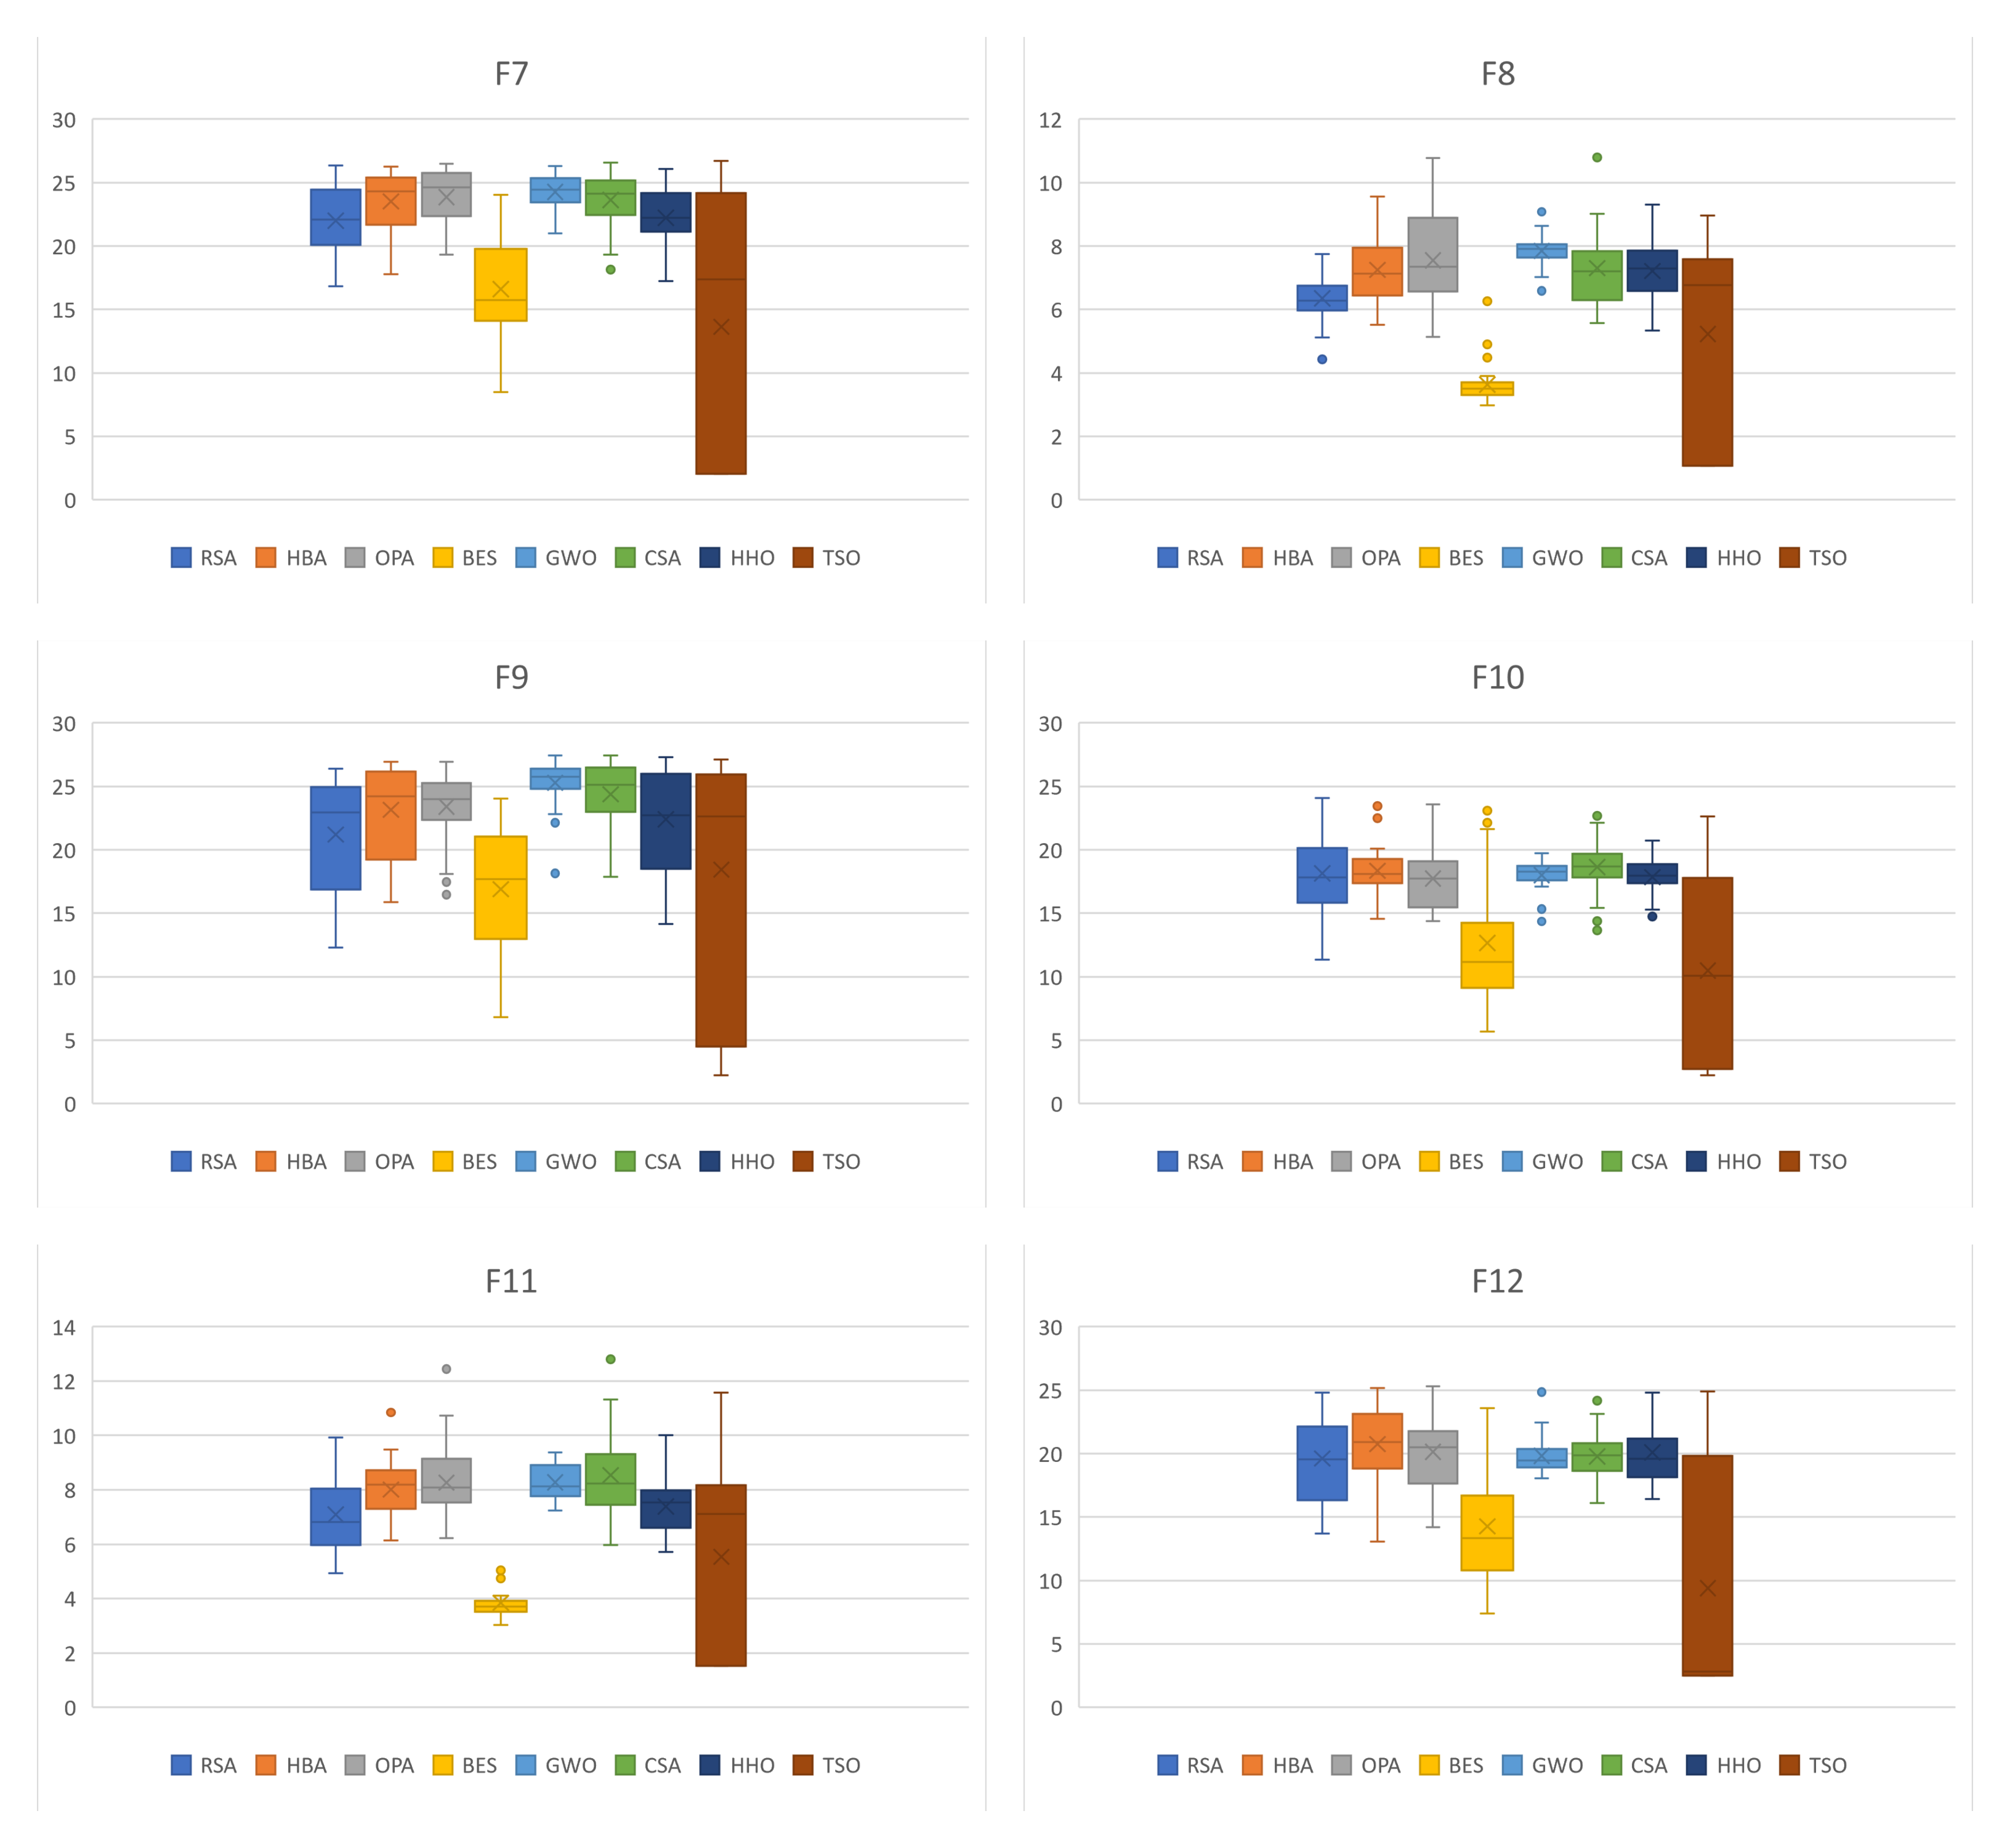
\includegraphics[width=\linewidth]{PSNR/Kapur/Dim8/PSNR_Dim8_Kapur_7_12.png}
	\end{subfigure}
	
	\begin{subfigure}{0.4\textwidth}
		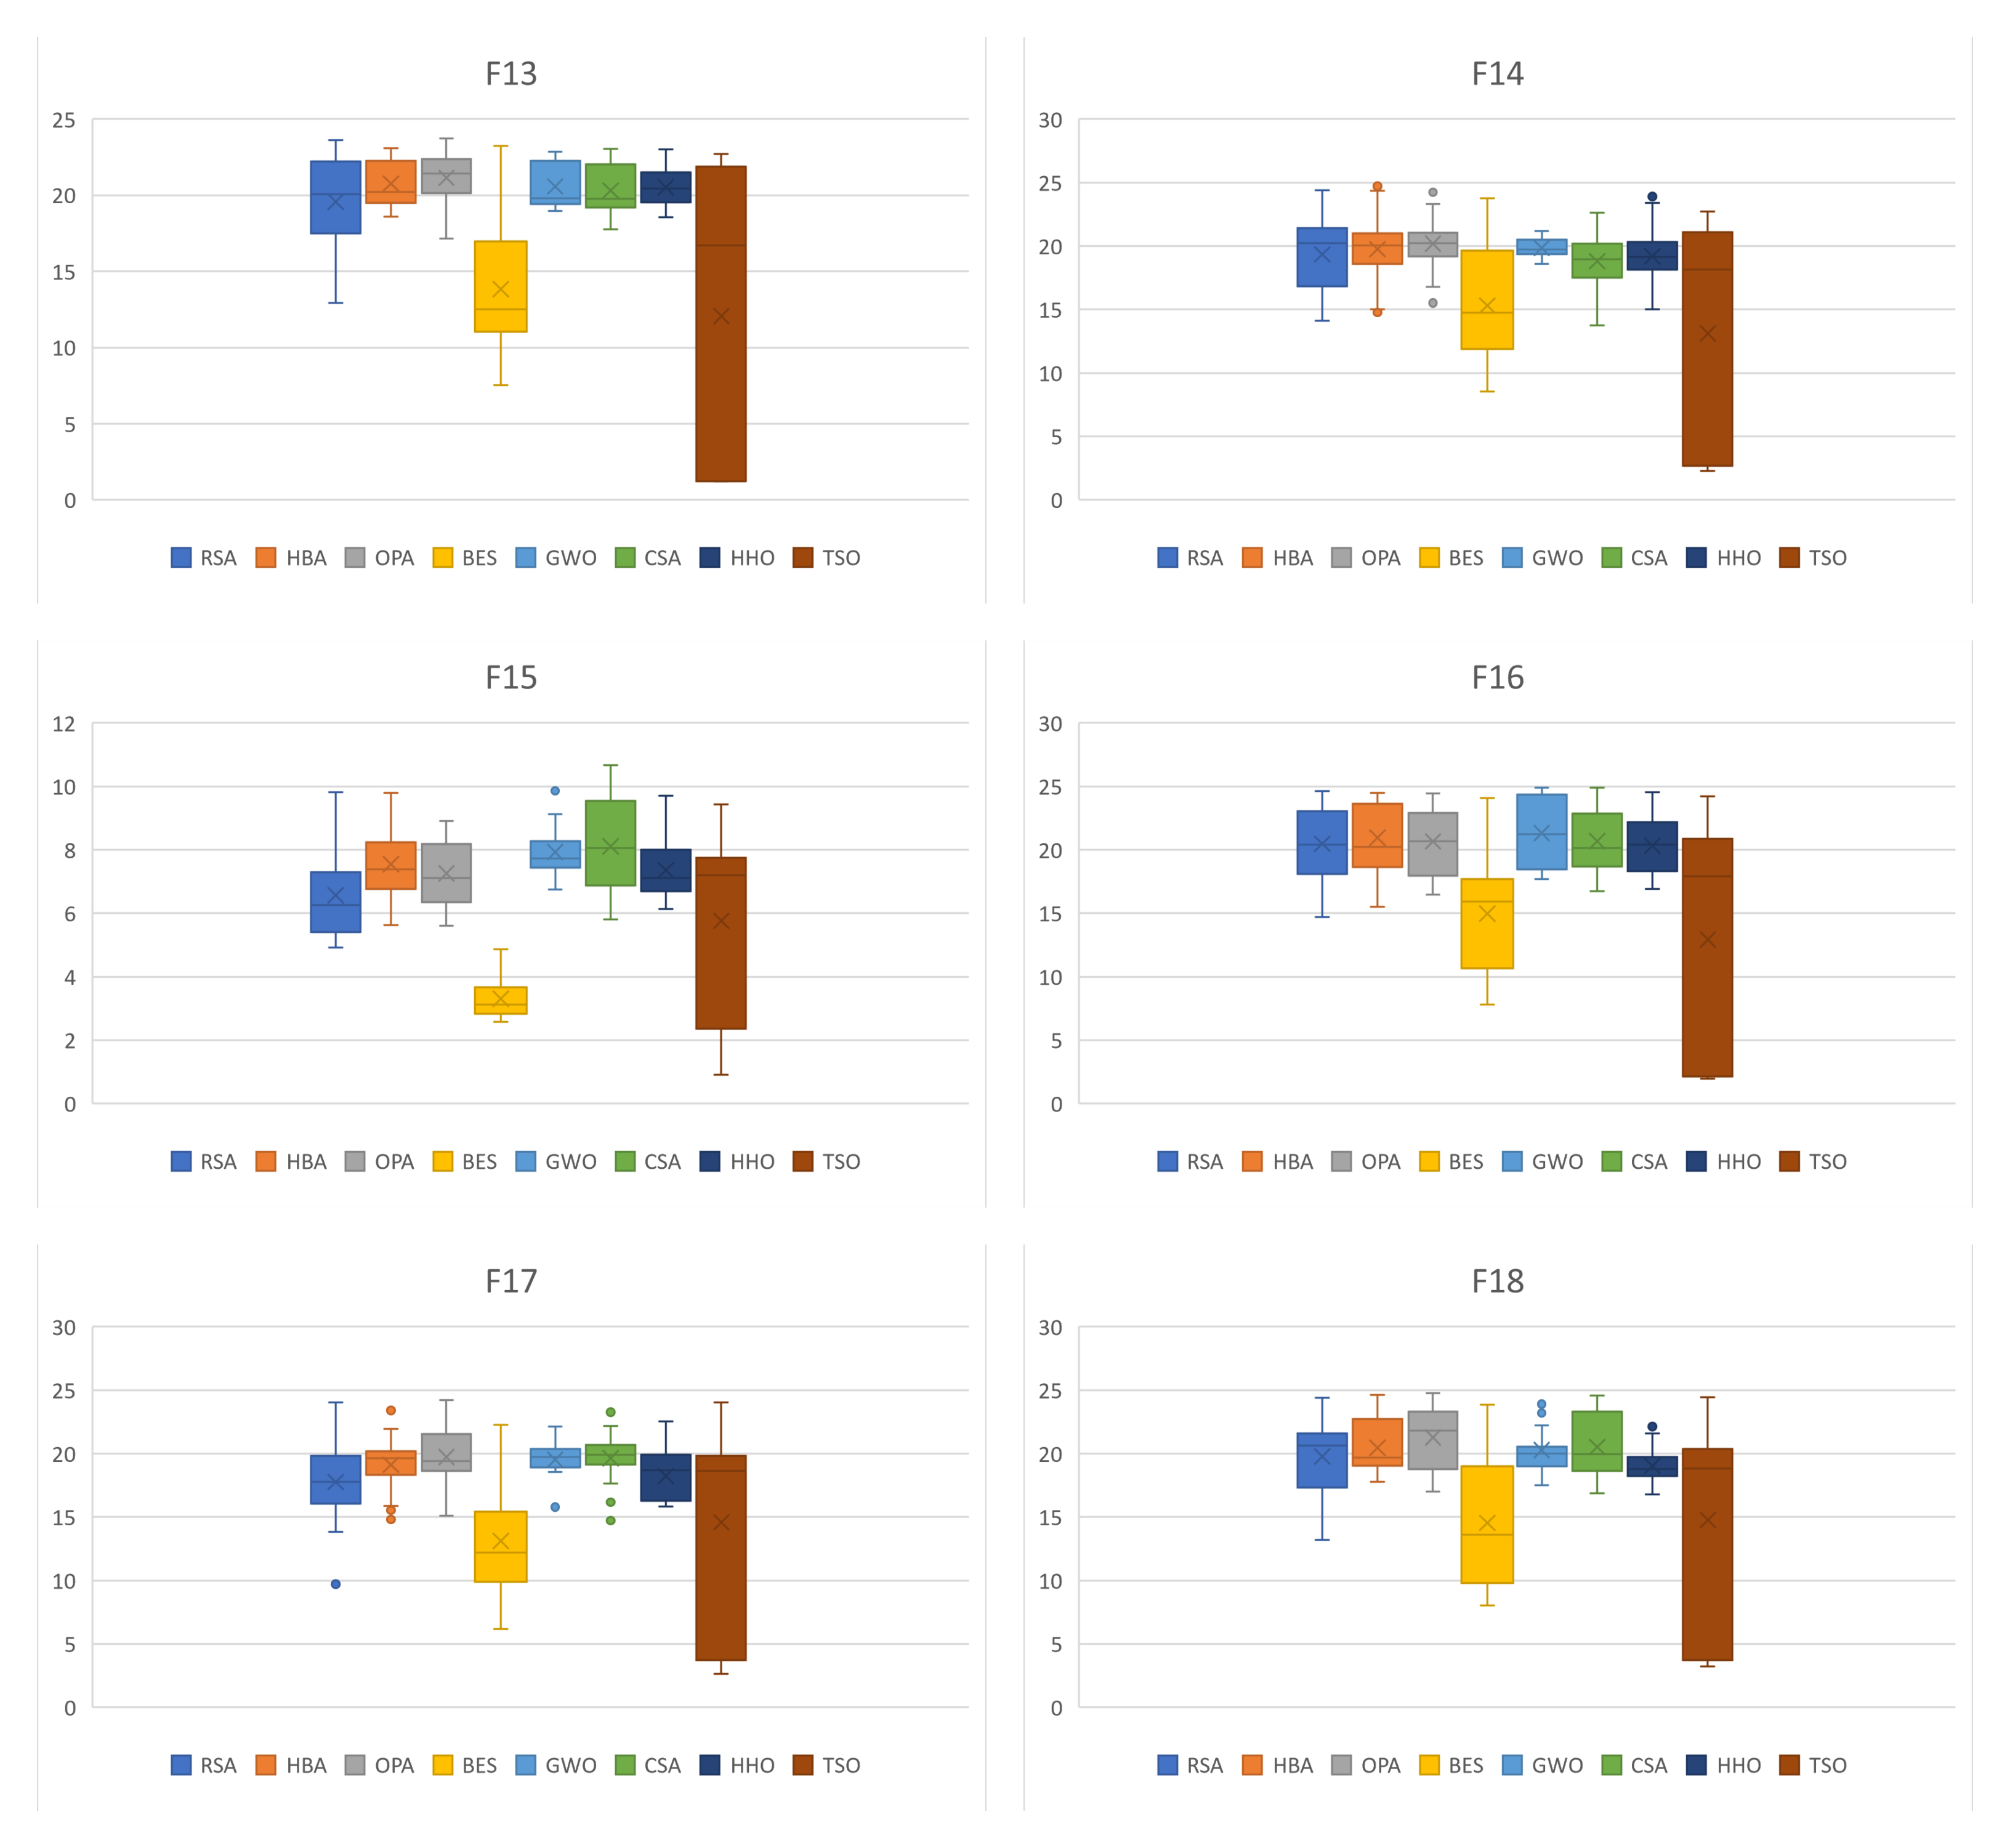
\includegraphics[width=\linewidth]{PSNR/Kapur/Dim8/PSNR_Dim8_Kapur_13_18.png}
	\end{subfigure}
	
	\begin{subfigure}{0.4\textwidth}
		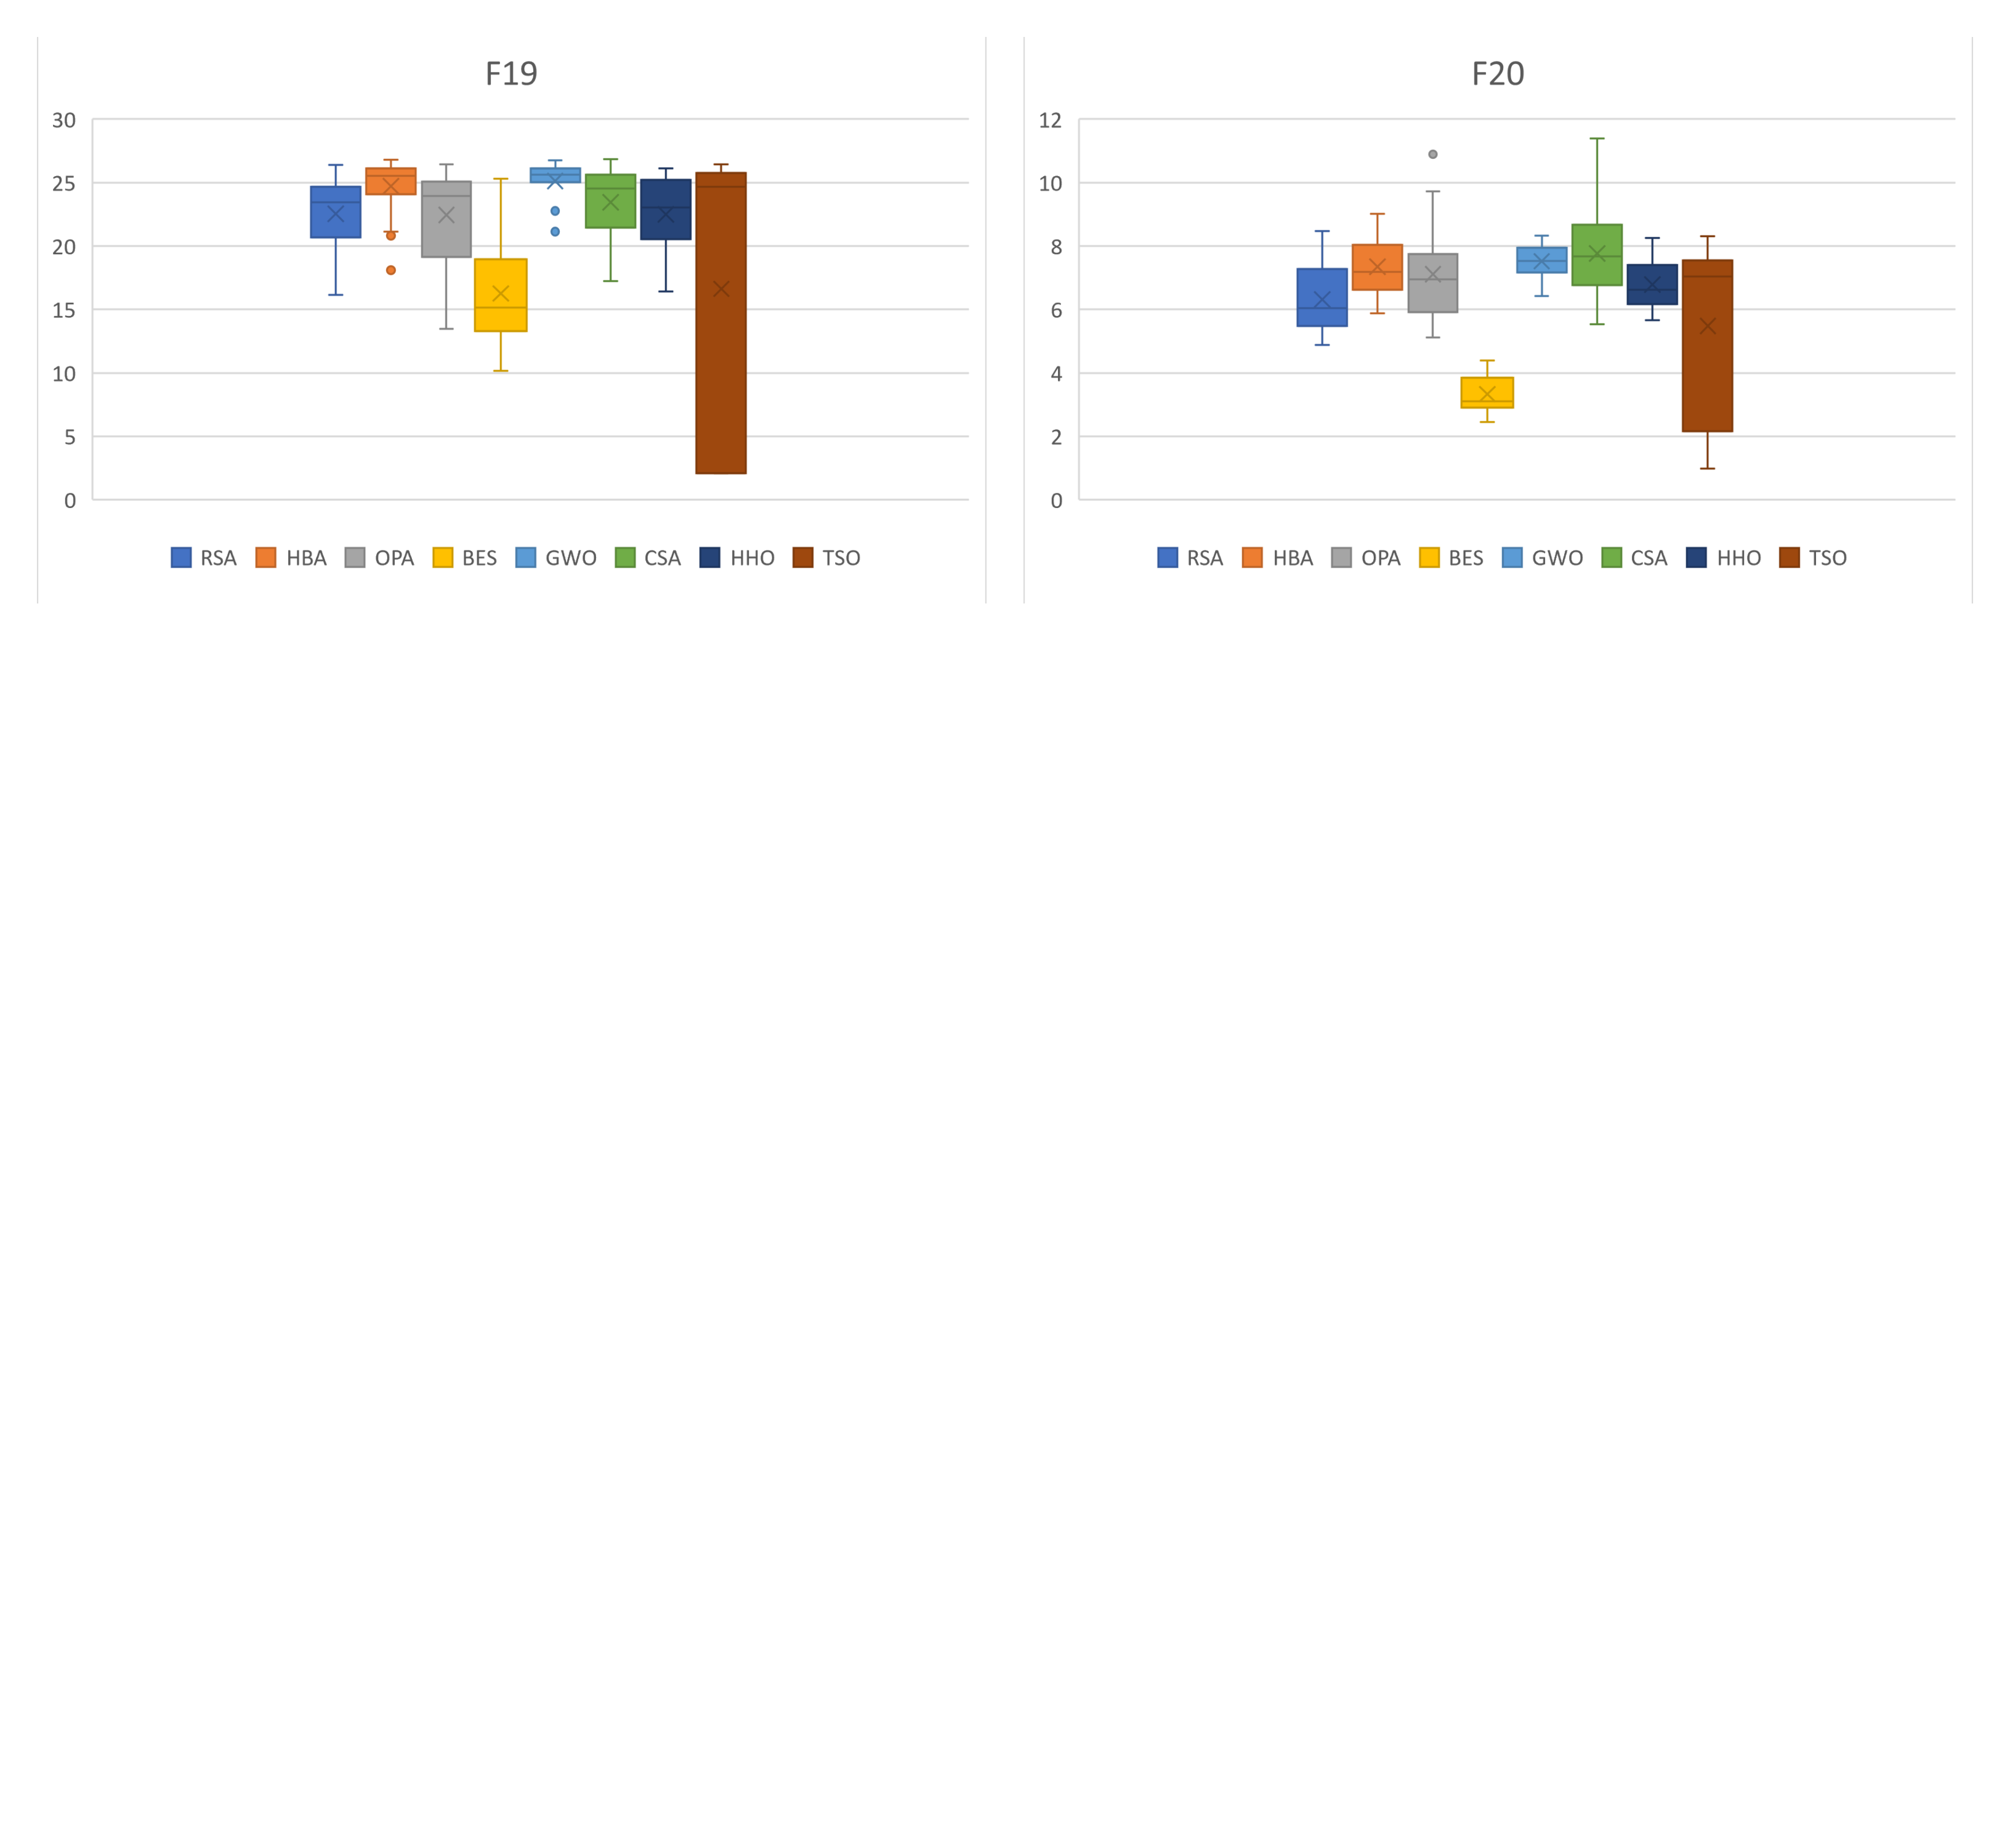
\includegraphics[width=\linewidth]{PSNR/Kapur/Dim8/PSNR_Dim8_Kapur_19_20.png}
		\vspace{-120pt} % Ajusta este valor según sea necesario
		% Elimina o ajusta el \vspace si es necesario. Aquí se ha eliminado para evitar solapamientos.
	\end{subfigure}
	\caption{Boxplot de los valores PSNR por cada imagen en la dimensión 8, desde la imagen 1 hasta la imagen 20, Función Entropía de Kapur.}
	\label{fig:imagenes_dim8_1_20}    
\end{figure}

\subsubsection{Dimensión 9}
\begin{itemize}
\item RSA: Este algoritmo ha mostrado consistentemente medianas de PSNR en el rango medio a medio-alto, con una variabilidad moderada en todas las imágenes. Esto sugiere un rendimiento confiable y una calidad de imagen generalmente buena.
	
\item HBA: Ha mantenido un rendimiento similar al RSA en términos de mediana de PSNR, con variabilidad moderada, lo cual indica un rendimiento sólido.
	
\item OPA: Ha exhibido una mediana de PSNR en el rango medio en todas las imágenes, con variabilidad moderada, indicando un rendimiento estable.
	
\item BES: Ha mostrado consistentemente las medianas de PSNR más bajas y una alta variabilidad, lo que indica un rendimiento inferior en comparación con los otros algoritmos.
	
\item GWO: Aunque no siempre ha tenido la mediana más alta de PSNR, su rendimiento ha sido sólido con una variabilidad relativamente baja en todas las imágenes. Esto sugiere que el GWO es confiable y ofrece una calidad de imagen consistente, clasificándolo entre los algoritmos de mejor rendimiento.
	
\item CSA: Este algoritmo ha tenido medianas de PSNR altas con una variabilidad moderada, lo que sugiere un rendimiento excelente y una calidad de imagen fiable.
	
\item HHO: Ha mostrado un rendimiento muy similar al CSA, con medianas de PSNR altas y variabilidad moderada, lo que también indica una calidad de imagen alta y consistente.
	
\item TSO: A pesar de tener las medianas más altas de PSNR, que señalan la mejor calidad de imagen teórica, la alta variabilidad sugiere que su rendimiento es inconsistente en comparación con los demás.
	
\end{itemize}
En resumen, el GWO se ha destacado por su confiabilidad y calidad de imagen consistente, haciéndolo uno de los mejores algoritmos junto con el CSA y el HHO. Estos tres algoritmos demuestran ser opciones robustas para aplicaciones que dependen de la alta calidad de la imagen y la consistencia. El TSO, aunque tiene el potencial de alta calidad, requiere consideración debido a su variabilidad. El BES parece ser el menos favorable en términos de rendimiento global. Los algoritmos RSA, HBA, y OPA proporcionan un rendimiento intermedio con una calidad de imagen fiable y consistentemente buena.
%% Dimension 9
\begin{figure}[htbp]
	\centering
	\begin{subfigure}{0.4\textwidth}
		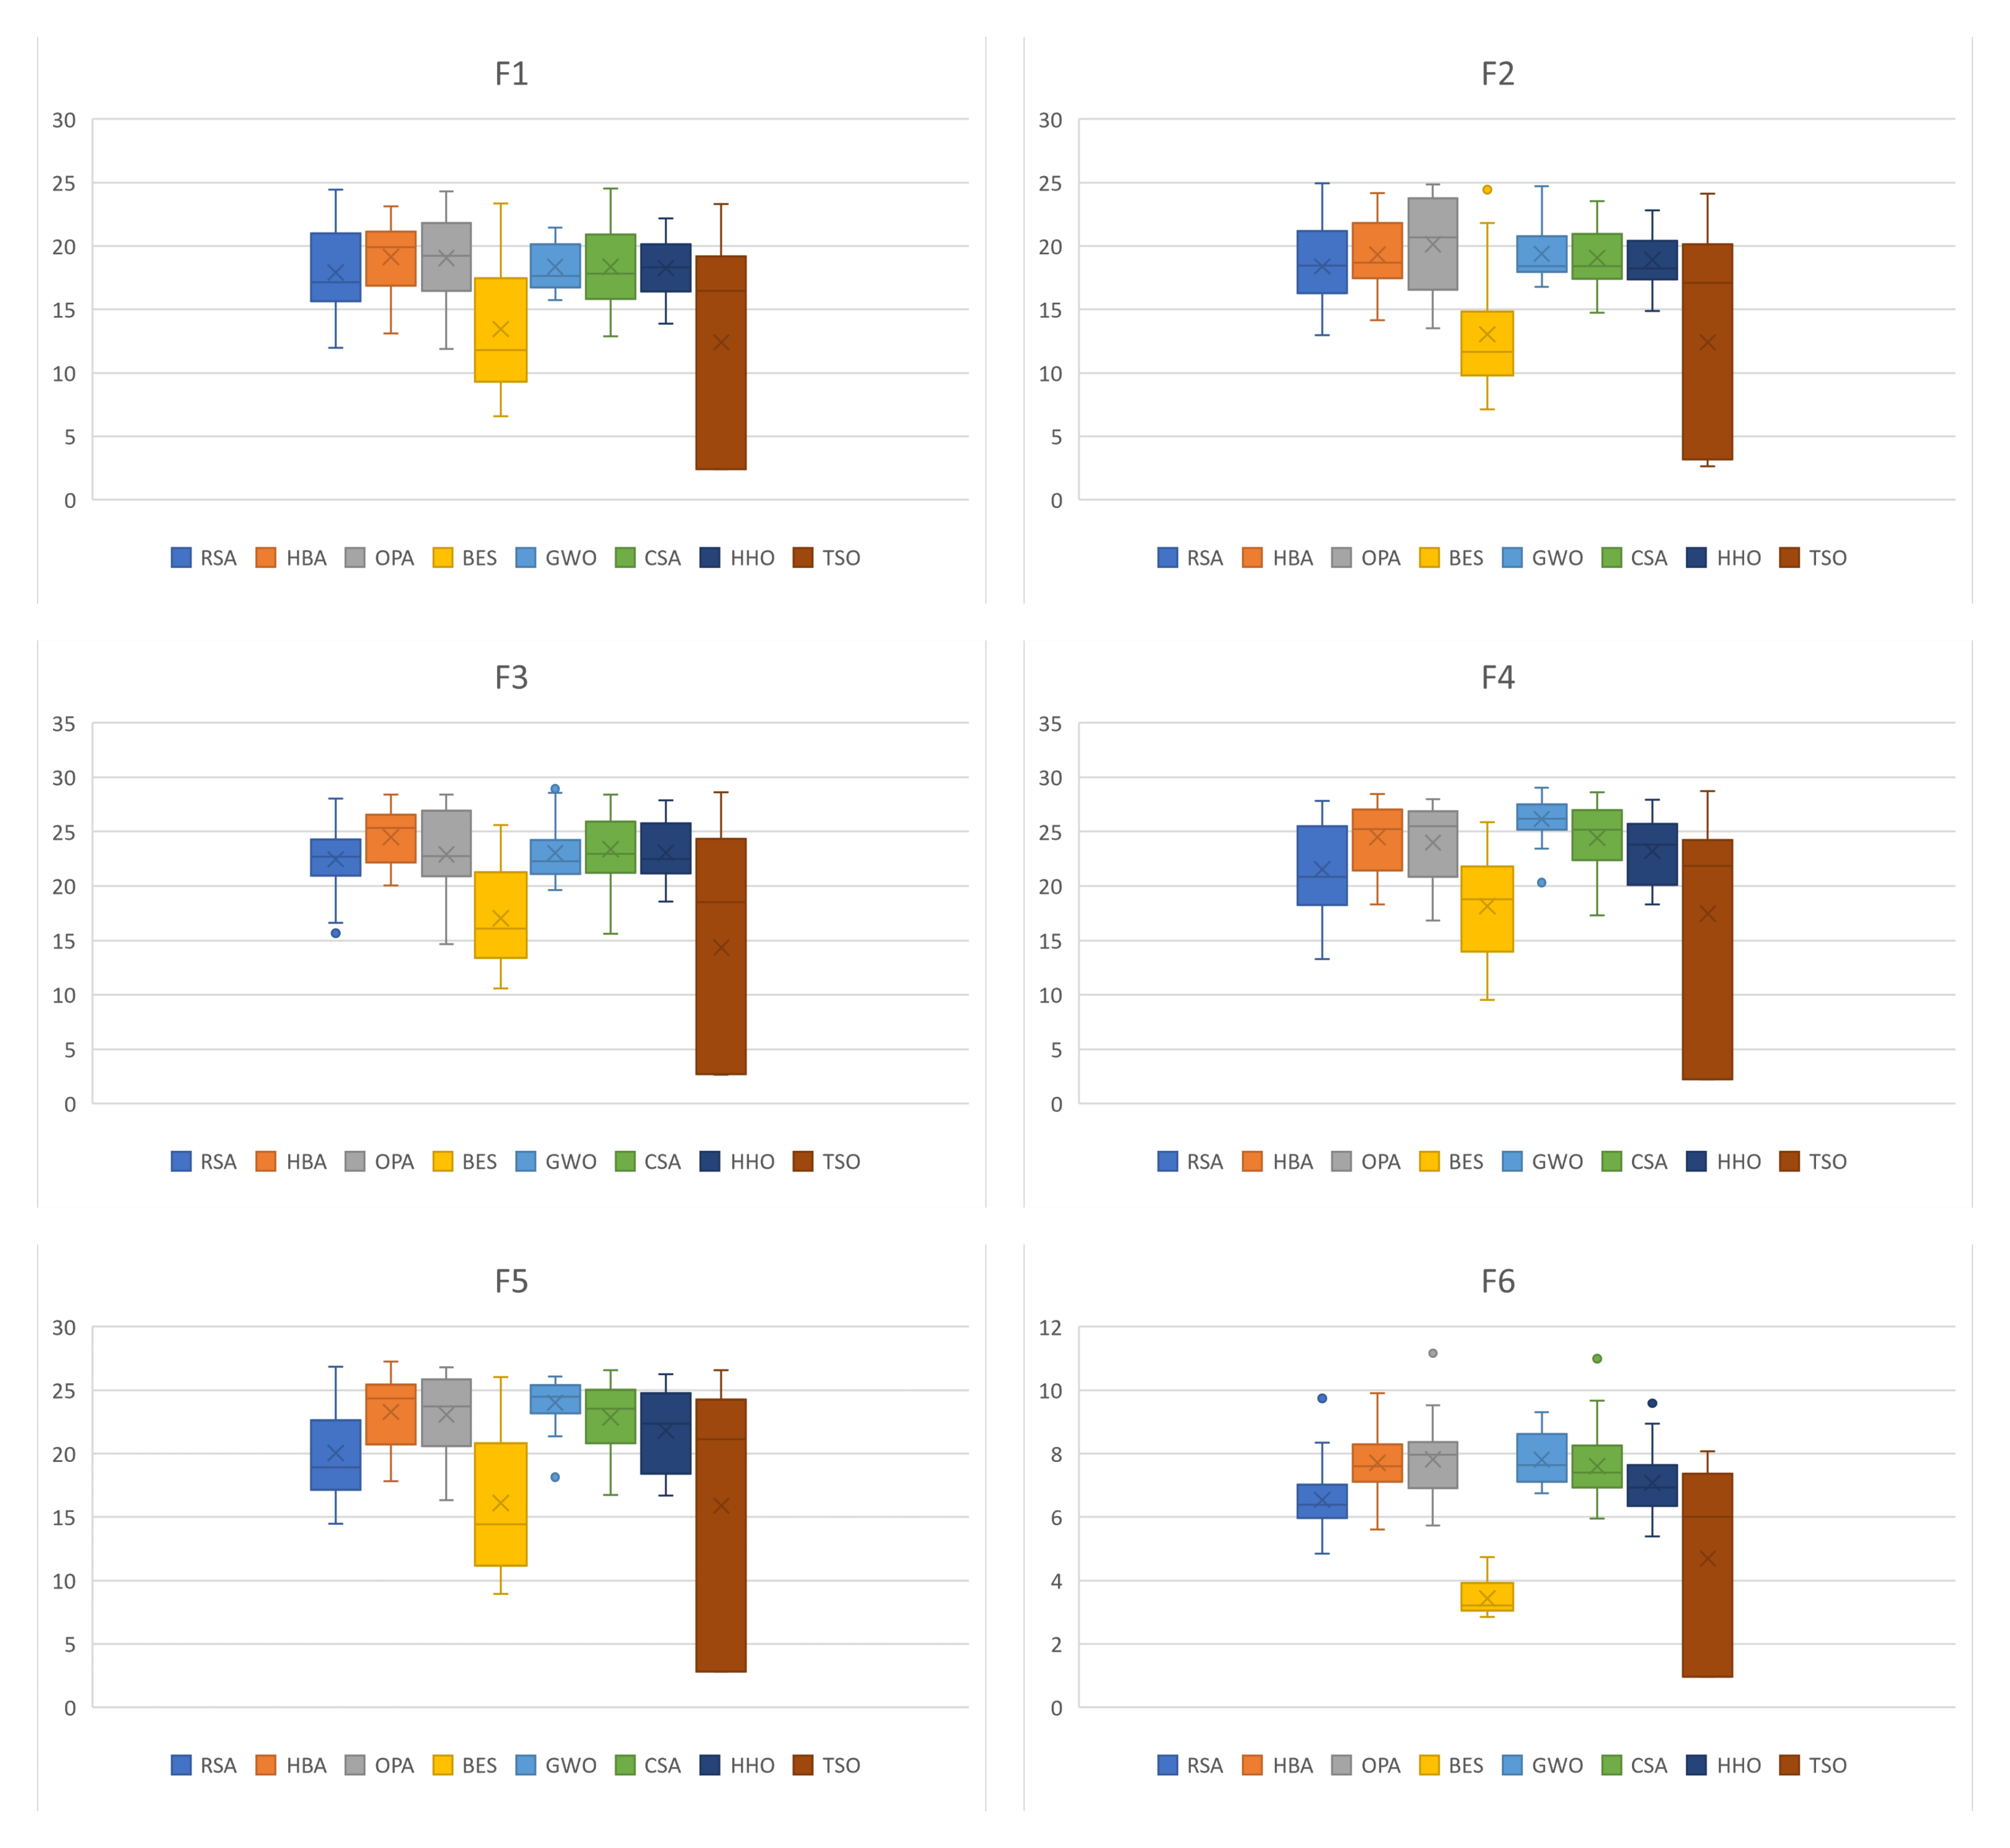
\includegraphics[width=\linewidth]{PSNR/Kapur/Dim9/PSNR_Dim9_Kapur_1_6.png}
	\end{subfigure}
	
	\begin{subfigure}{0.4\textwidth}
		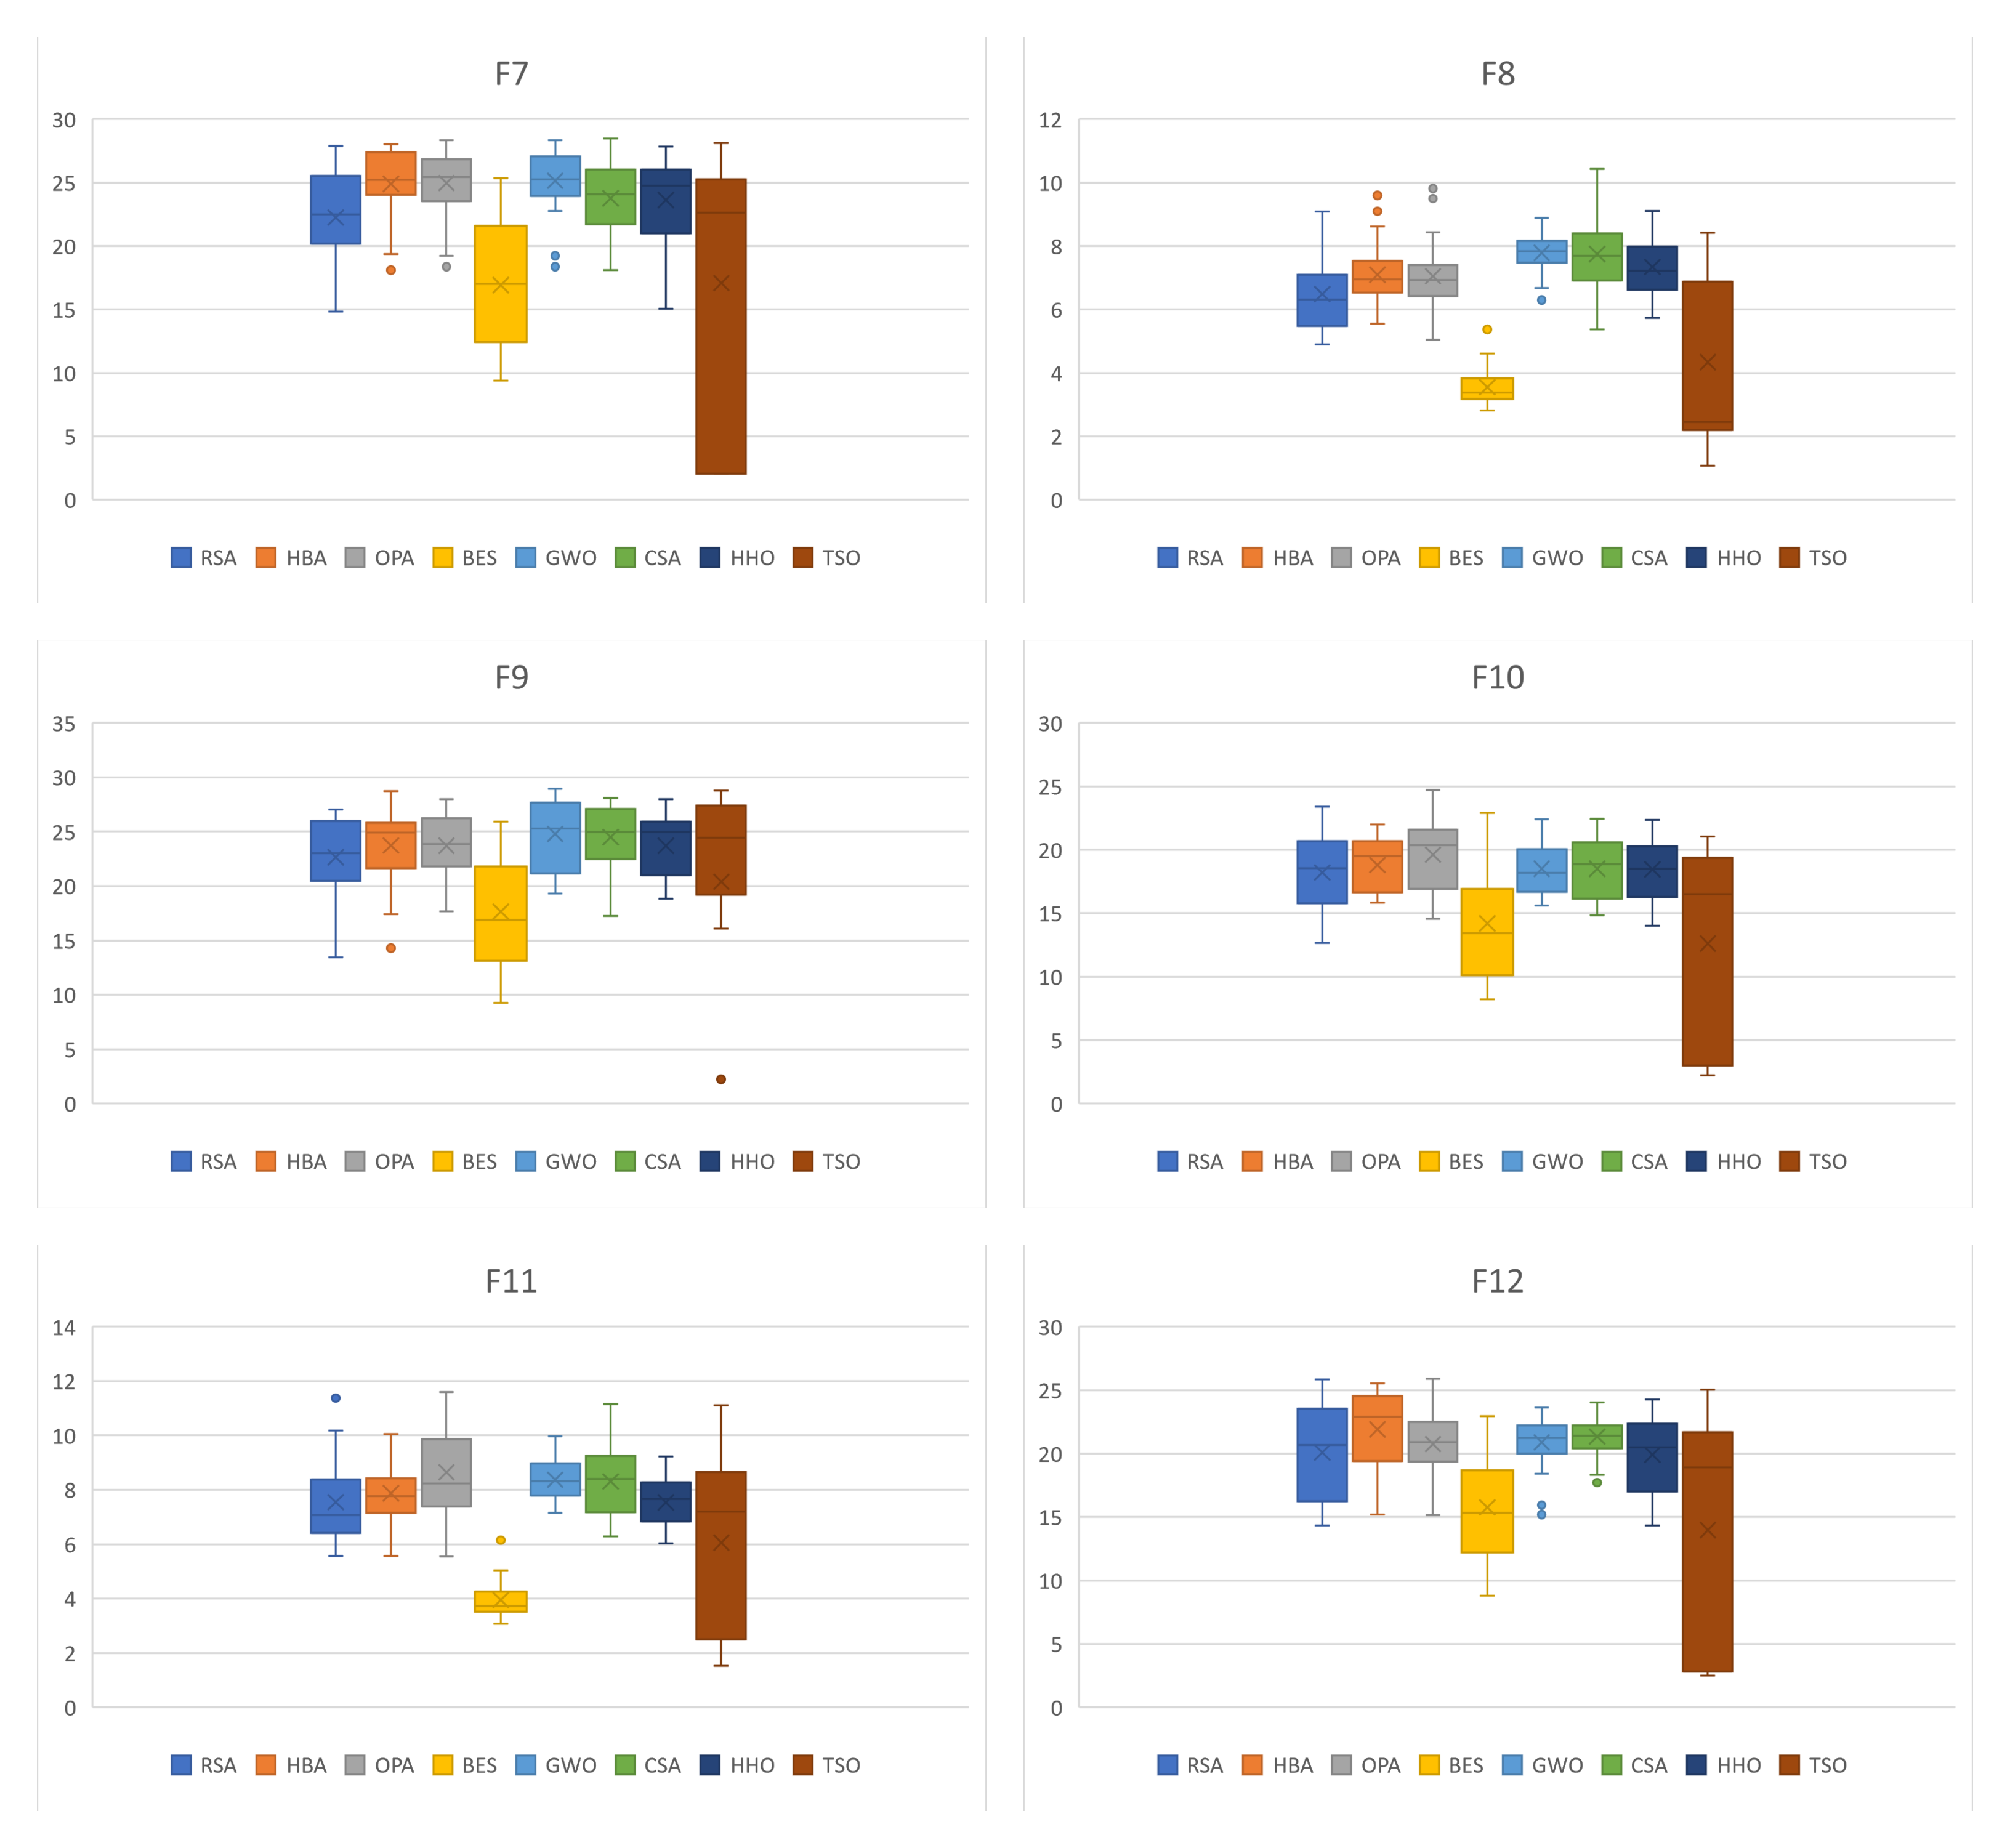
\includegraphics[width=\linewidth]{PSNR/Kapur/Dim9/PSNR_Dim9_Kapur_7_12.png}
	\end{subfigure}
	\begin{subfigure}{0.4\textwidth}
		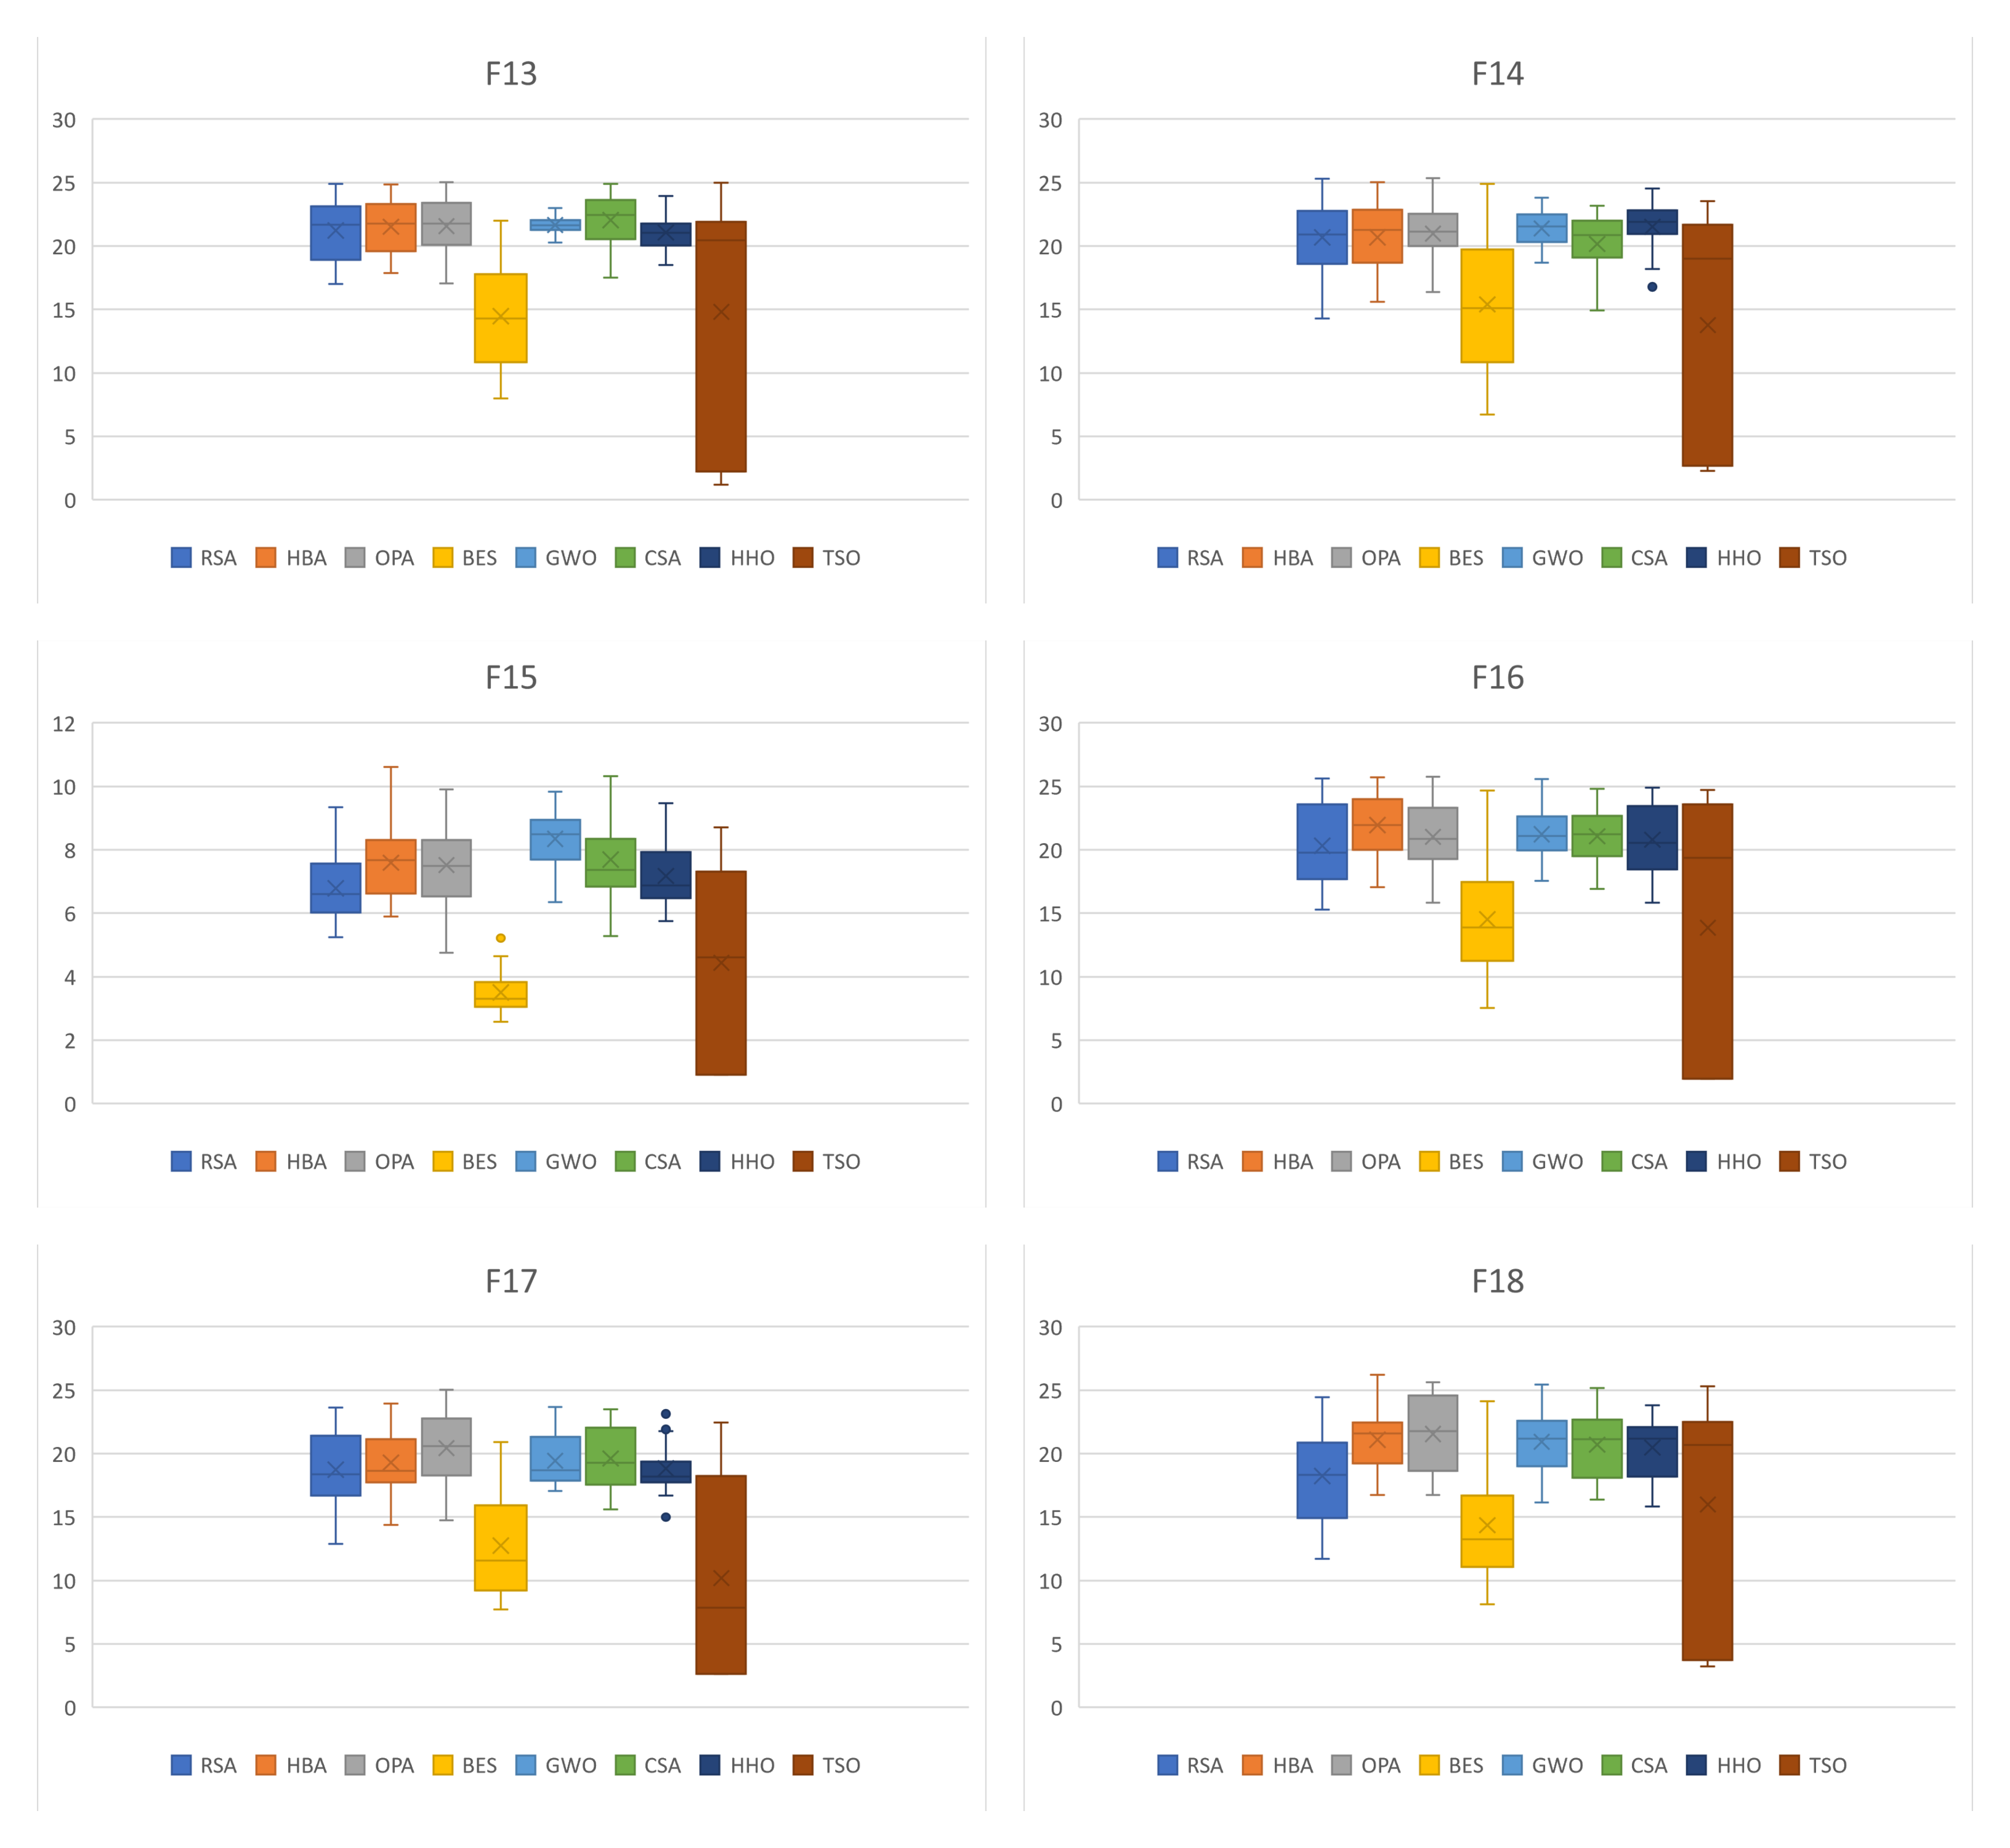
\includegraphics[width=\linewidth]{PSNR/Kapur/Dim9/PSNR_Dim9_Kapur_13_18.png}
		%\vspace{-150pt} % Ajusta este valor según sea necesario
	\end{subfigure}   
	\begin{subfigure}{0.4\textwidth}
		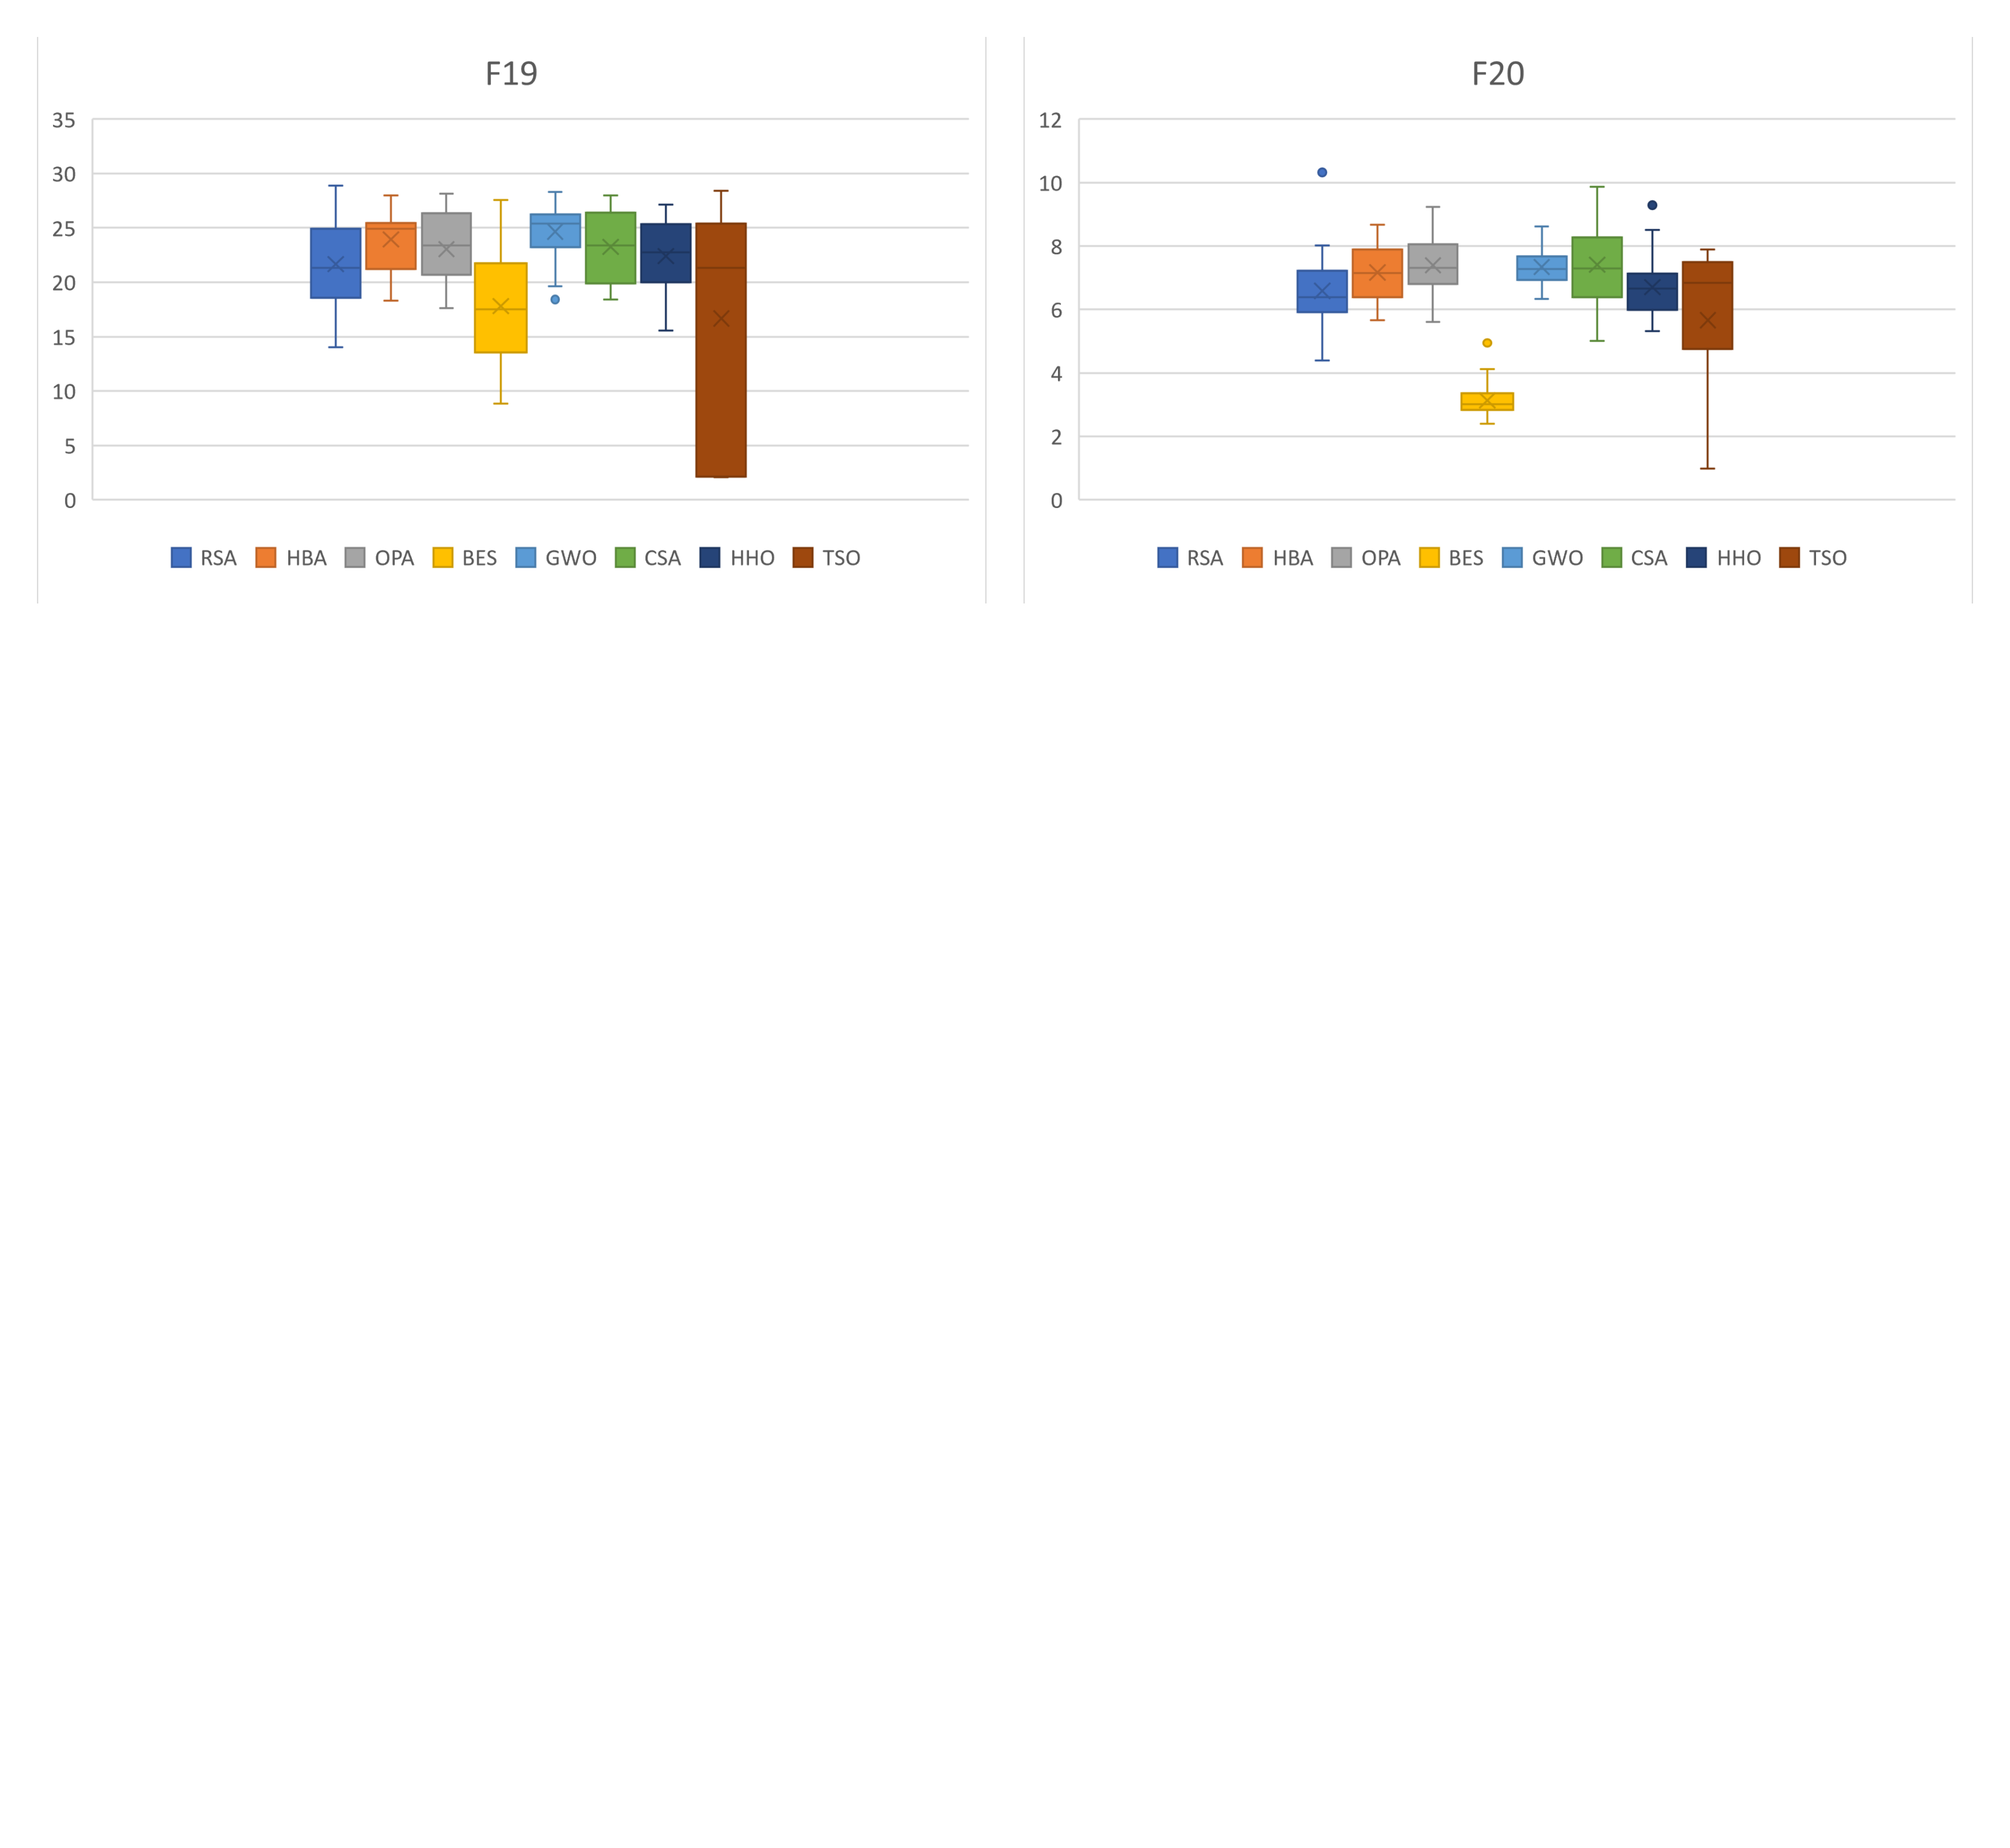
\includegraphics[width=\linewidth]{PSNR/Kapur/Dim9/PSNR_Dim9_Kapur_19_20.png}
		\vspace{-120pt} % Ajusta este valor según sea necesario
	\end{subfigure}
	\caption{Boxplot de los valores PSNR por cada imagen en la dimensión 9, desde la imagen 1 hasta la imagen 20,Función Entropía de Kapur}
	\label{fig:imagenes}    
\end{figure}
\subsection{Resultados Función SSIM Entropía de Kapur}
\subsubsection{Dimensión 7}
\begin{itemize}
\item RSA: A lo largo de las cuatro últimas imágenes, RSA ha mantenido una mediana de SSIM en el rango medio con una variabilidad moderada. Esto sugiere que RSA ofrece una calidad de imagen razonablemente buena y consistente en diferentes escenarios.
	
\item HBA ha demostrado una mediana de SSIM similar a RSA en estas imágenes, con variabilidad moderada. Esto indica un rendimiento comparable en términos de calidad de imagen en diferentes situaciones.
	
\item OPA ha exhibido una mediana de SSIM en el rango medio, similar a RSA y HBA, con variabilidad moderada. Esto sugiere una calidad de imagen consistente y razonablemente buena.
	
\item BES ha presentado la mediana más baja de SSIM en estas imágenes, lo que indica una calidad de imagen inferior en comparación con otros algoritmos. Además, la variabilidad es alta, lo que sugiere que su rendimiento puede ser menos consistente.
	
\item GWO ha mantenido una mediana de SSIM en el rango medio-alto en las últimas cuatro imágenes, con variabilidad relativamente baja. Esto indica que GWO ofrece un rendimiento robusto y consistente en términos de similitud estructural con la imagen de referencia.

\item CSA ha demostrado una mediana de SSIM alta con variabilidad moderada en estas imágenes. Esto sugiere un rendimiento sólido y una calidad de imagen confiable.
	
\item HHO ha presentado una mediana de SSIM y variabilidad similares a las de CSA, indicando un rendimiento robusto y fiable en términos de calidad de imagen.
	
\item TSO ha mostrado la mediana más alta de SSIM en estas imágenes, lo que indica la mejor similitud estructural con la imagen de referencia. Sin embargo, su variabilidad es significativa, lo que sugiere que su calidad de imagen puede variar ampliamente en diferentes escenarios.
	
\end{itemize}
\noindent En resumen, GWO, CSA y HHO se destacan por ofrecer un rendimiento fuerte y consistente en términos de similitud estructural con la imagen de referencia en las últimas cuatro imágenes. TSO, aunque muestra la calidad potencialmente más alta, es menos confiable debido a su variabilidad. BES parece ser el menos favorable en términos de calidad de imagen y consistencia. RSA, HBA y OPA proporcionan una calidad de imagen razonablemente buena y consistente en diferentes situaciones.
%% Boxplot de los valores SSIM por cada imagen en la dimensión 7, desde la imagen 1 hasta la imagen 20,Función Entropía de Kapur
\begin{figure}
	\centering
	
	\begin{subfigure}{0.4\textwidth}
		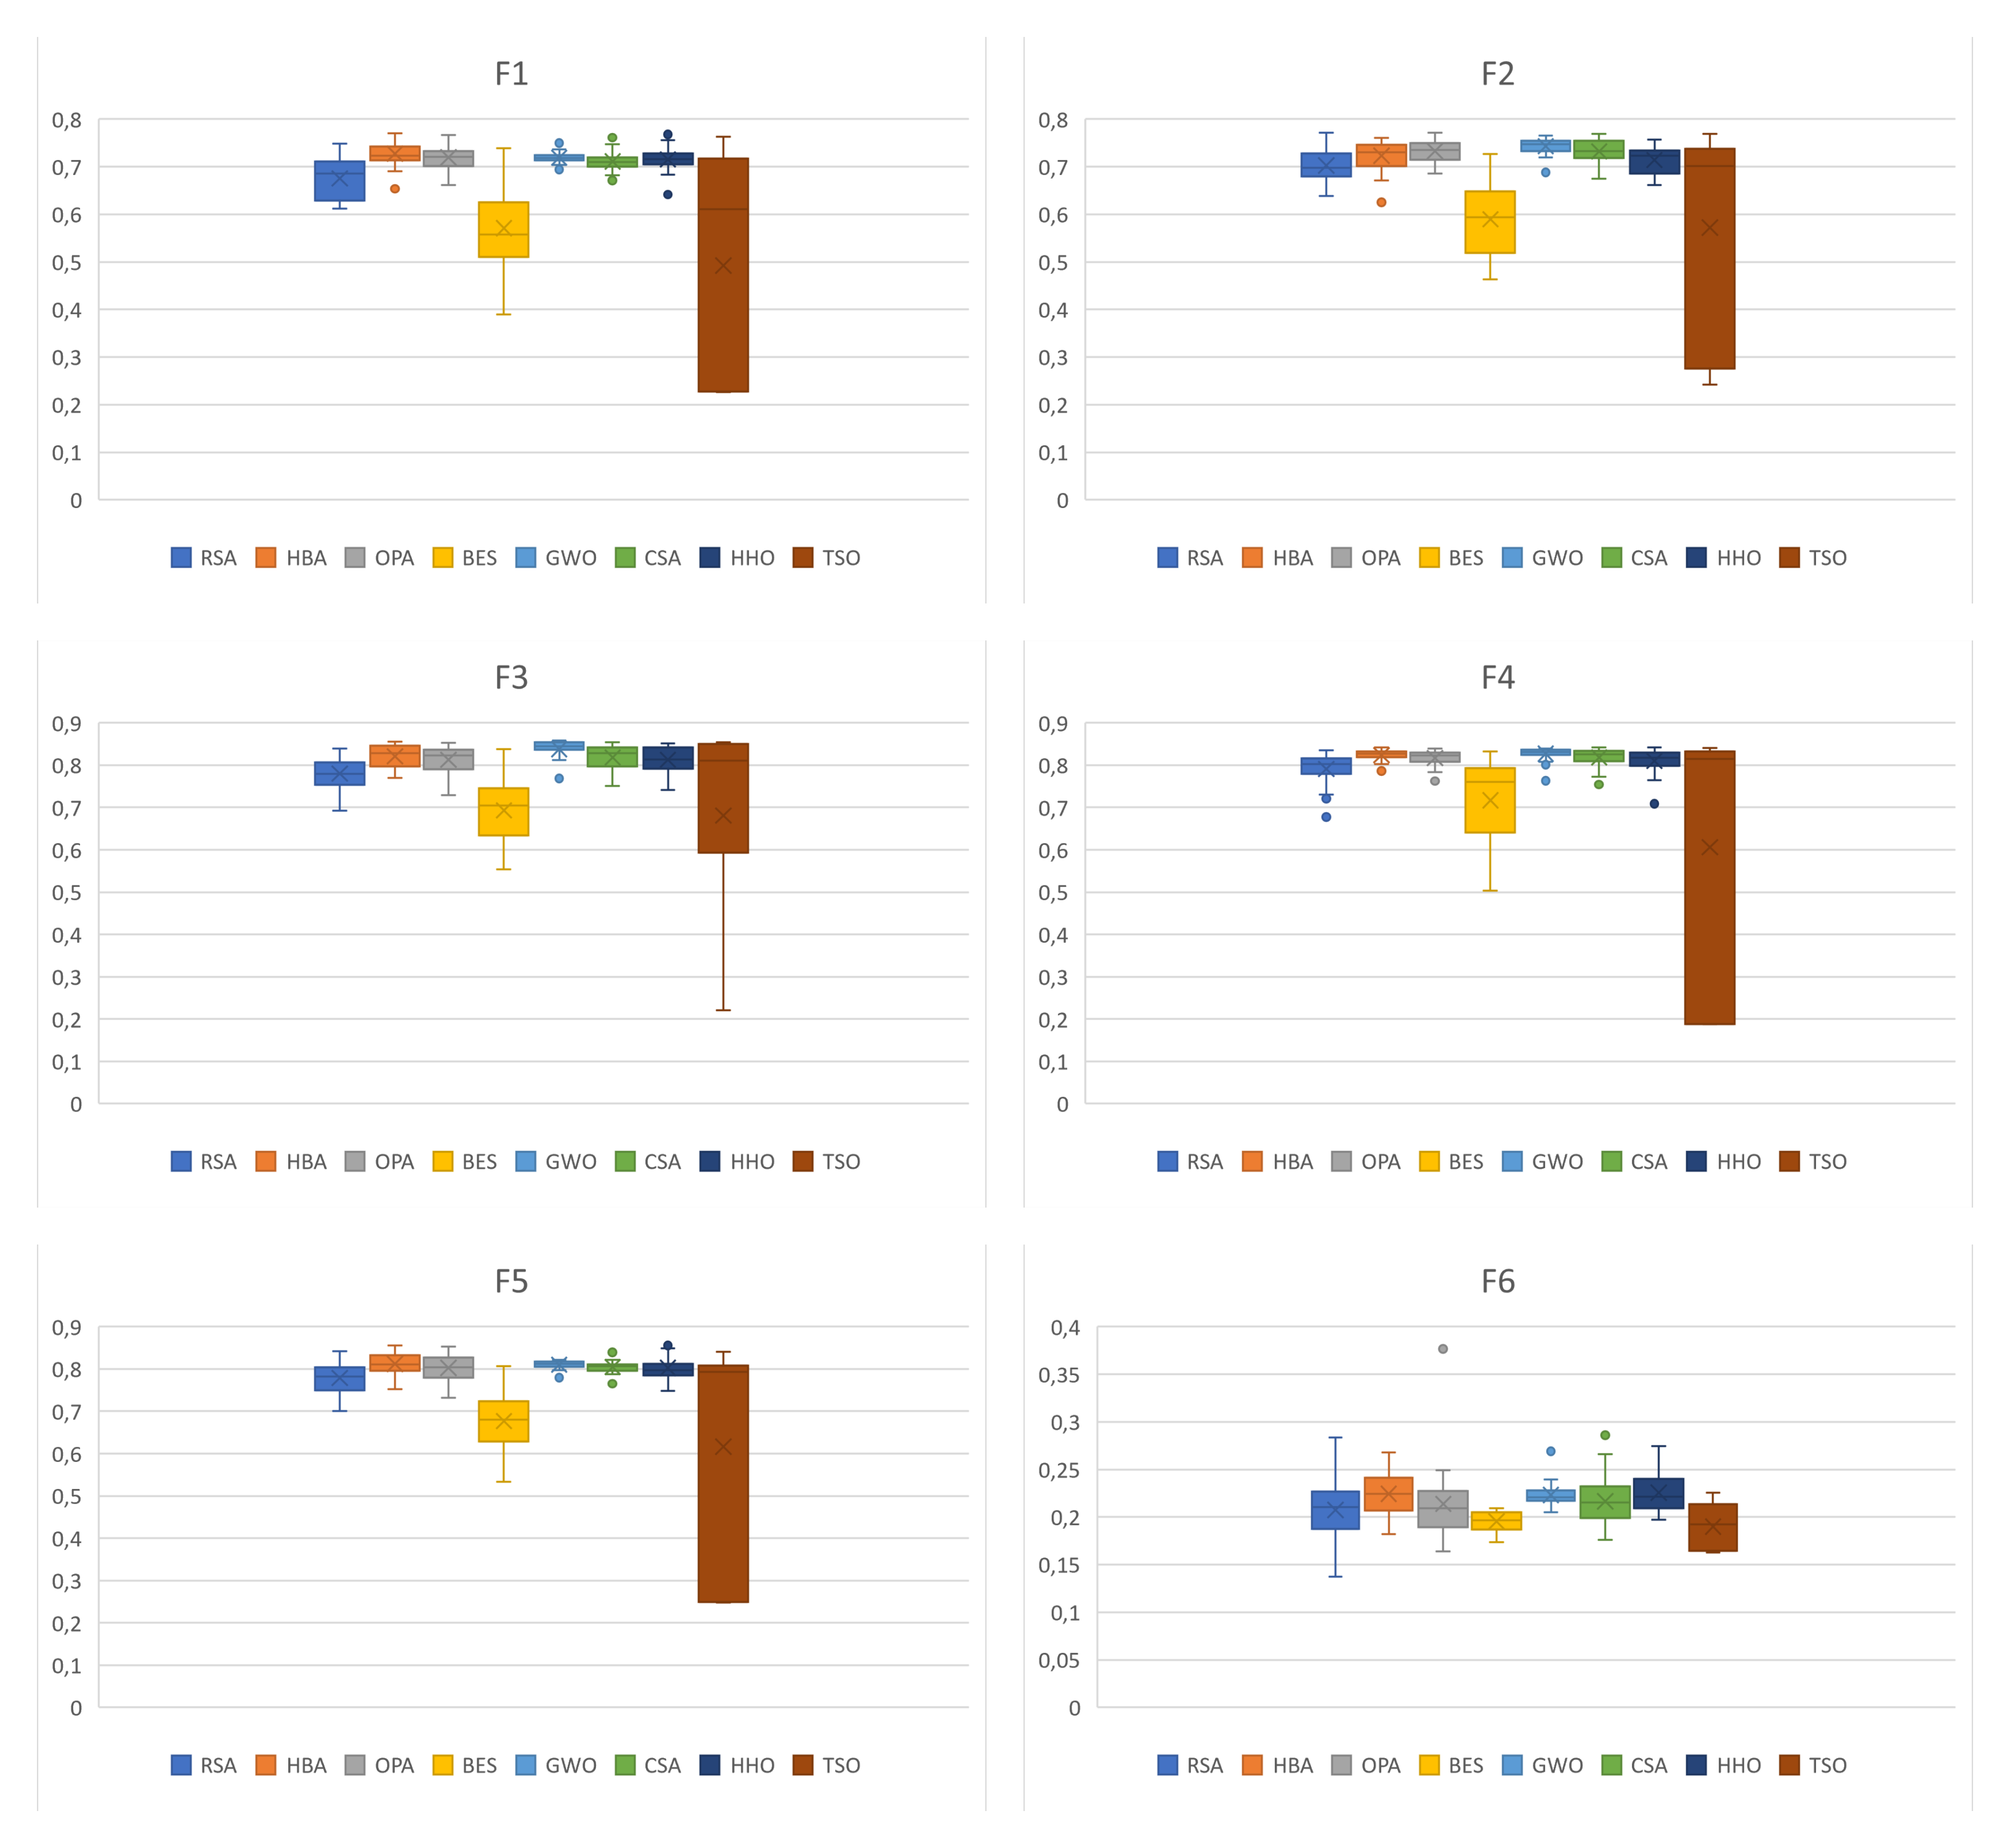
\includegraphics[width=\linewidth]{SSIM/Kapur/Dim7/SSIM_Dim7_Kapur_1_6.png}
	\end{subfigure}
	
	\begin{subfigure}{0.4\textwidth}
		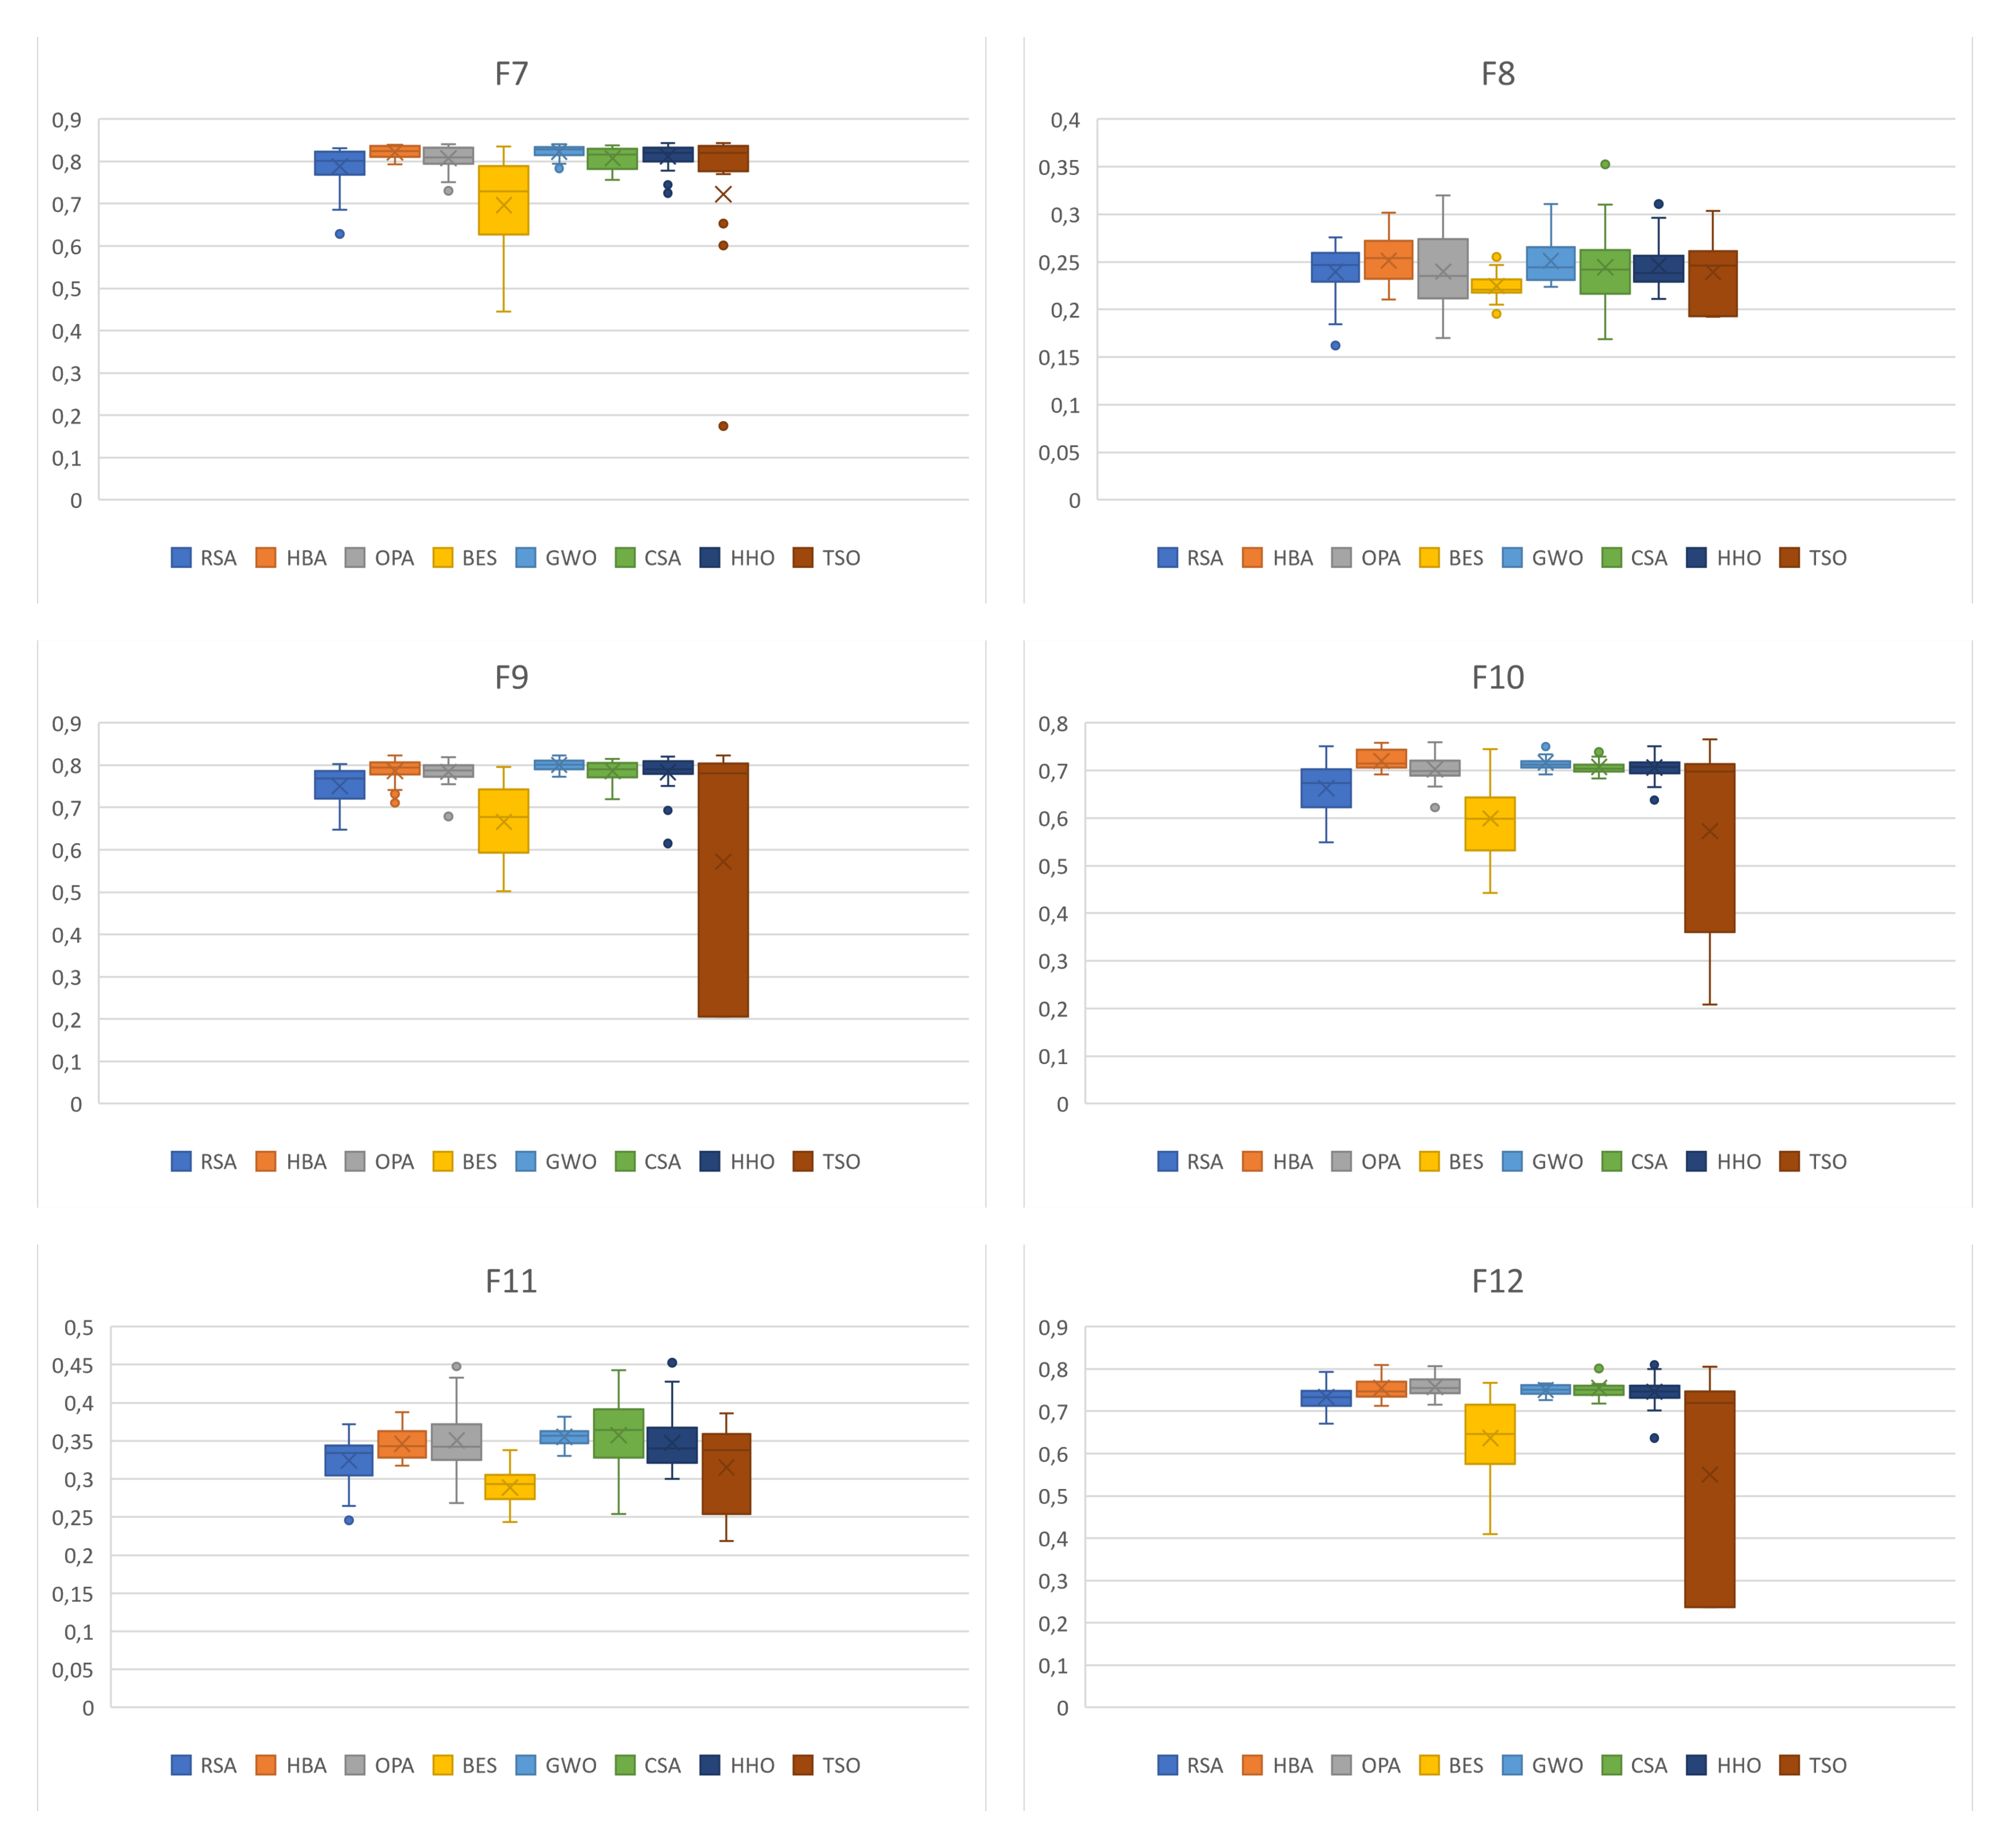
\includegraphics[width=\linewidth]{SSIM/Kapur/Dim7/SSIM_Dim7_Kapur_7_12.png}
	\end{subfigure}
	\begin{subfigure}{0.4\textwidth}
		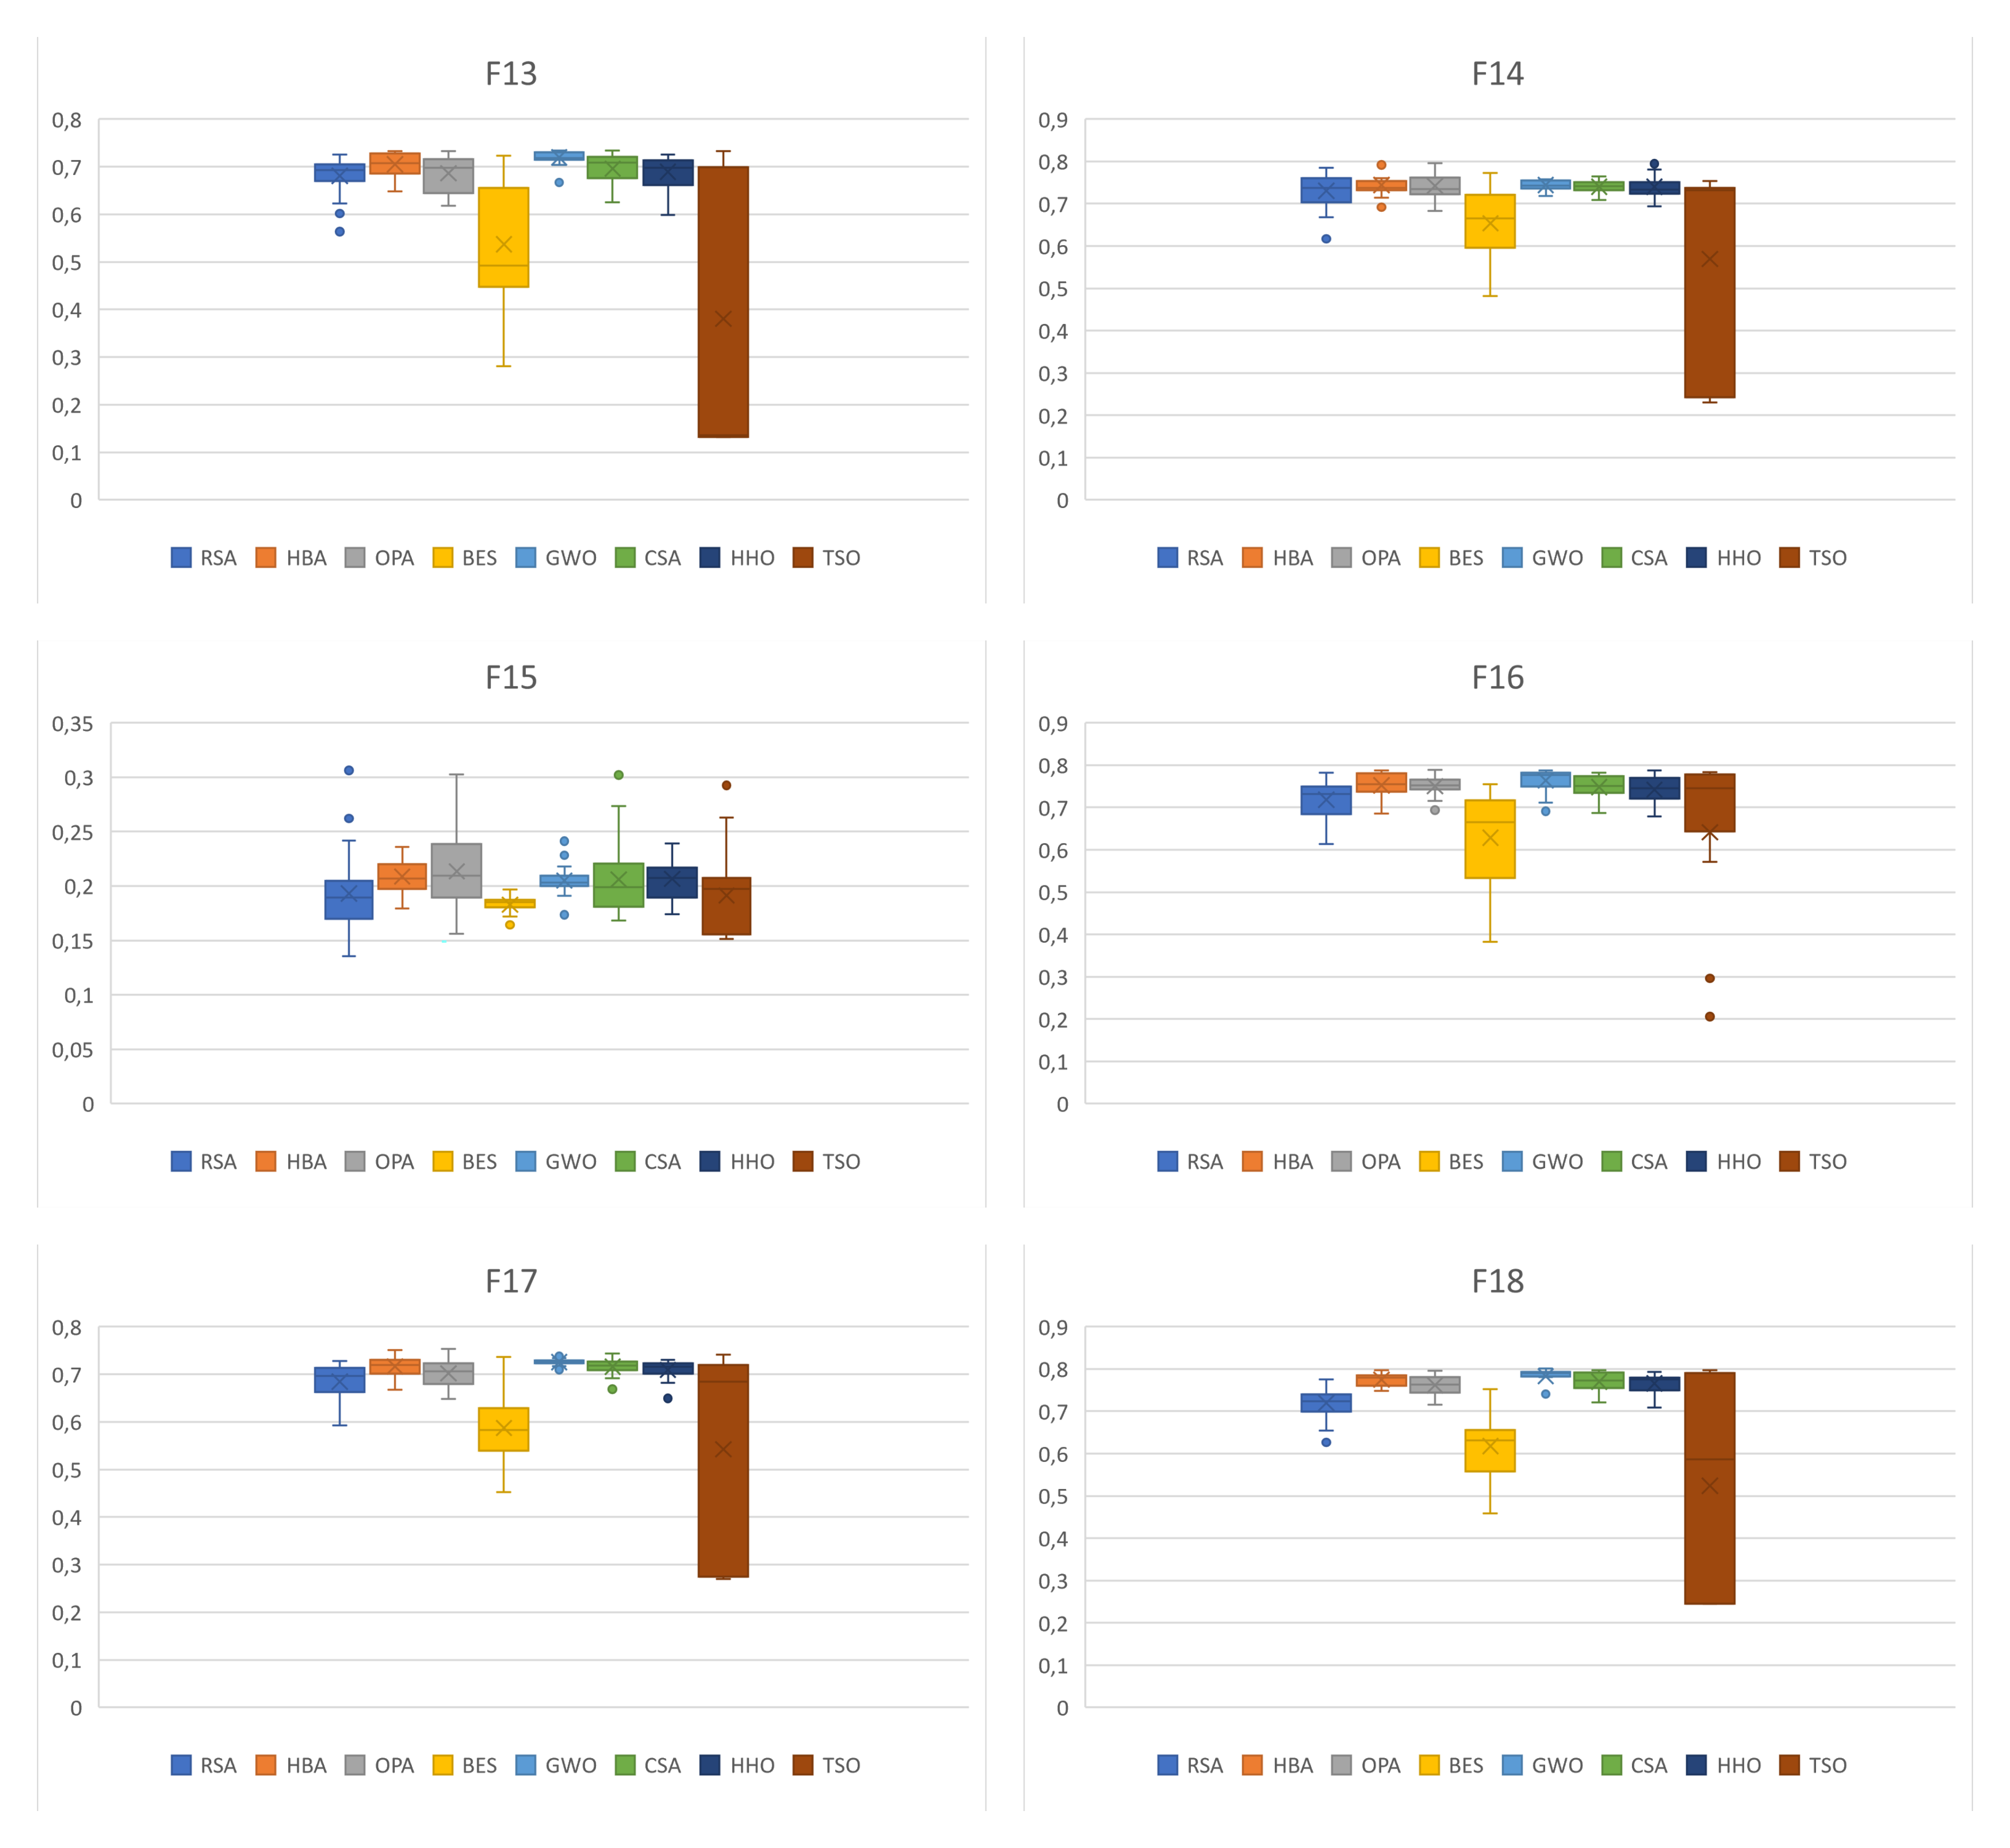
\includegraphics[width=\linewidth]{SSIM/Kapur/Dim7/SSIM_Dim7_Kapur_13_18.png}
		%\vspace{-150pt} % Ajusta este valor según sea necesario
	\end{subfigure}   
	\begin{subfigure}{0.4\textwidth}
		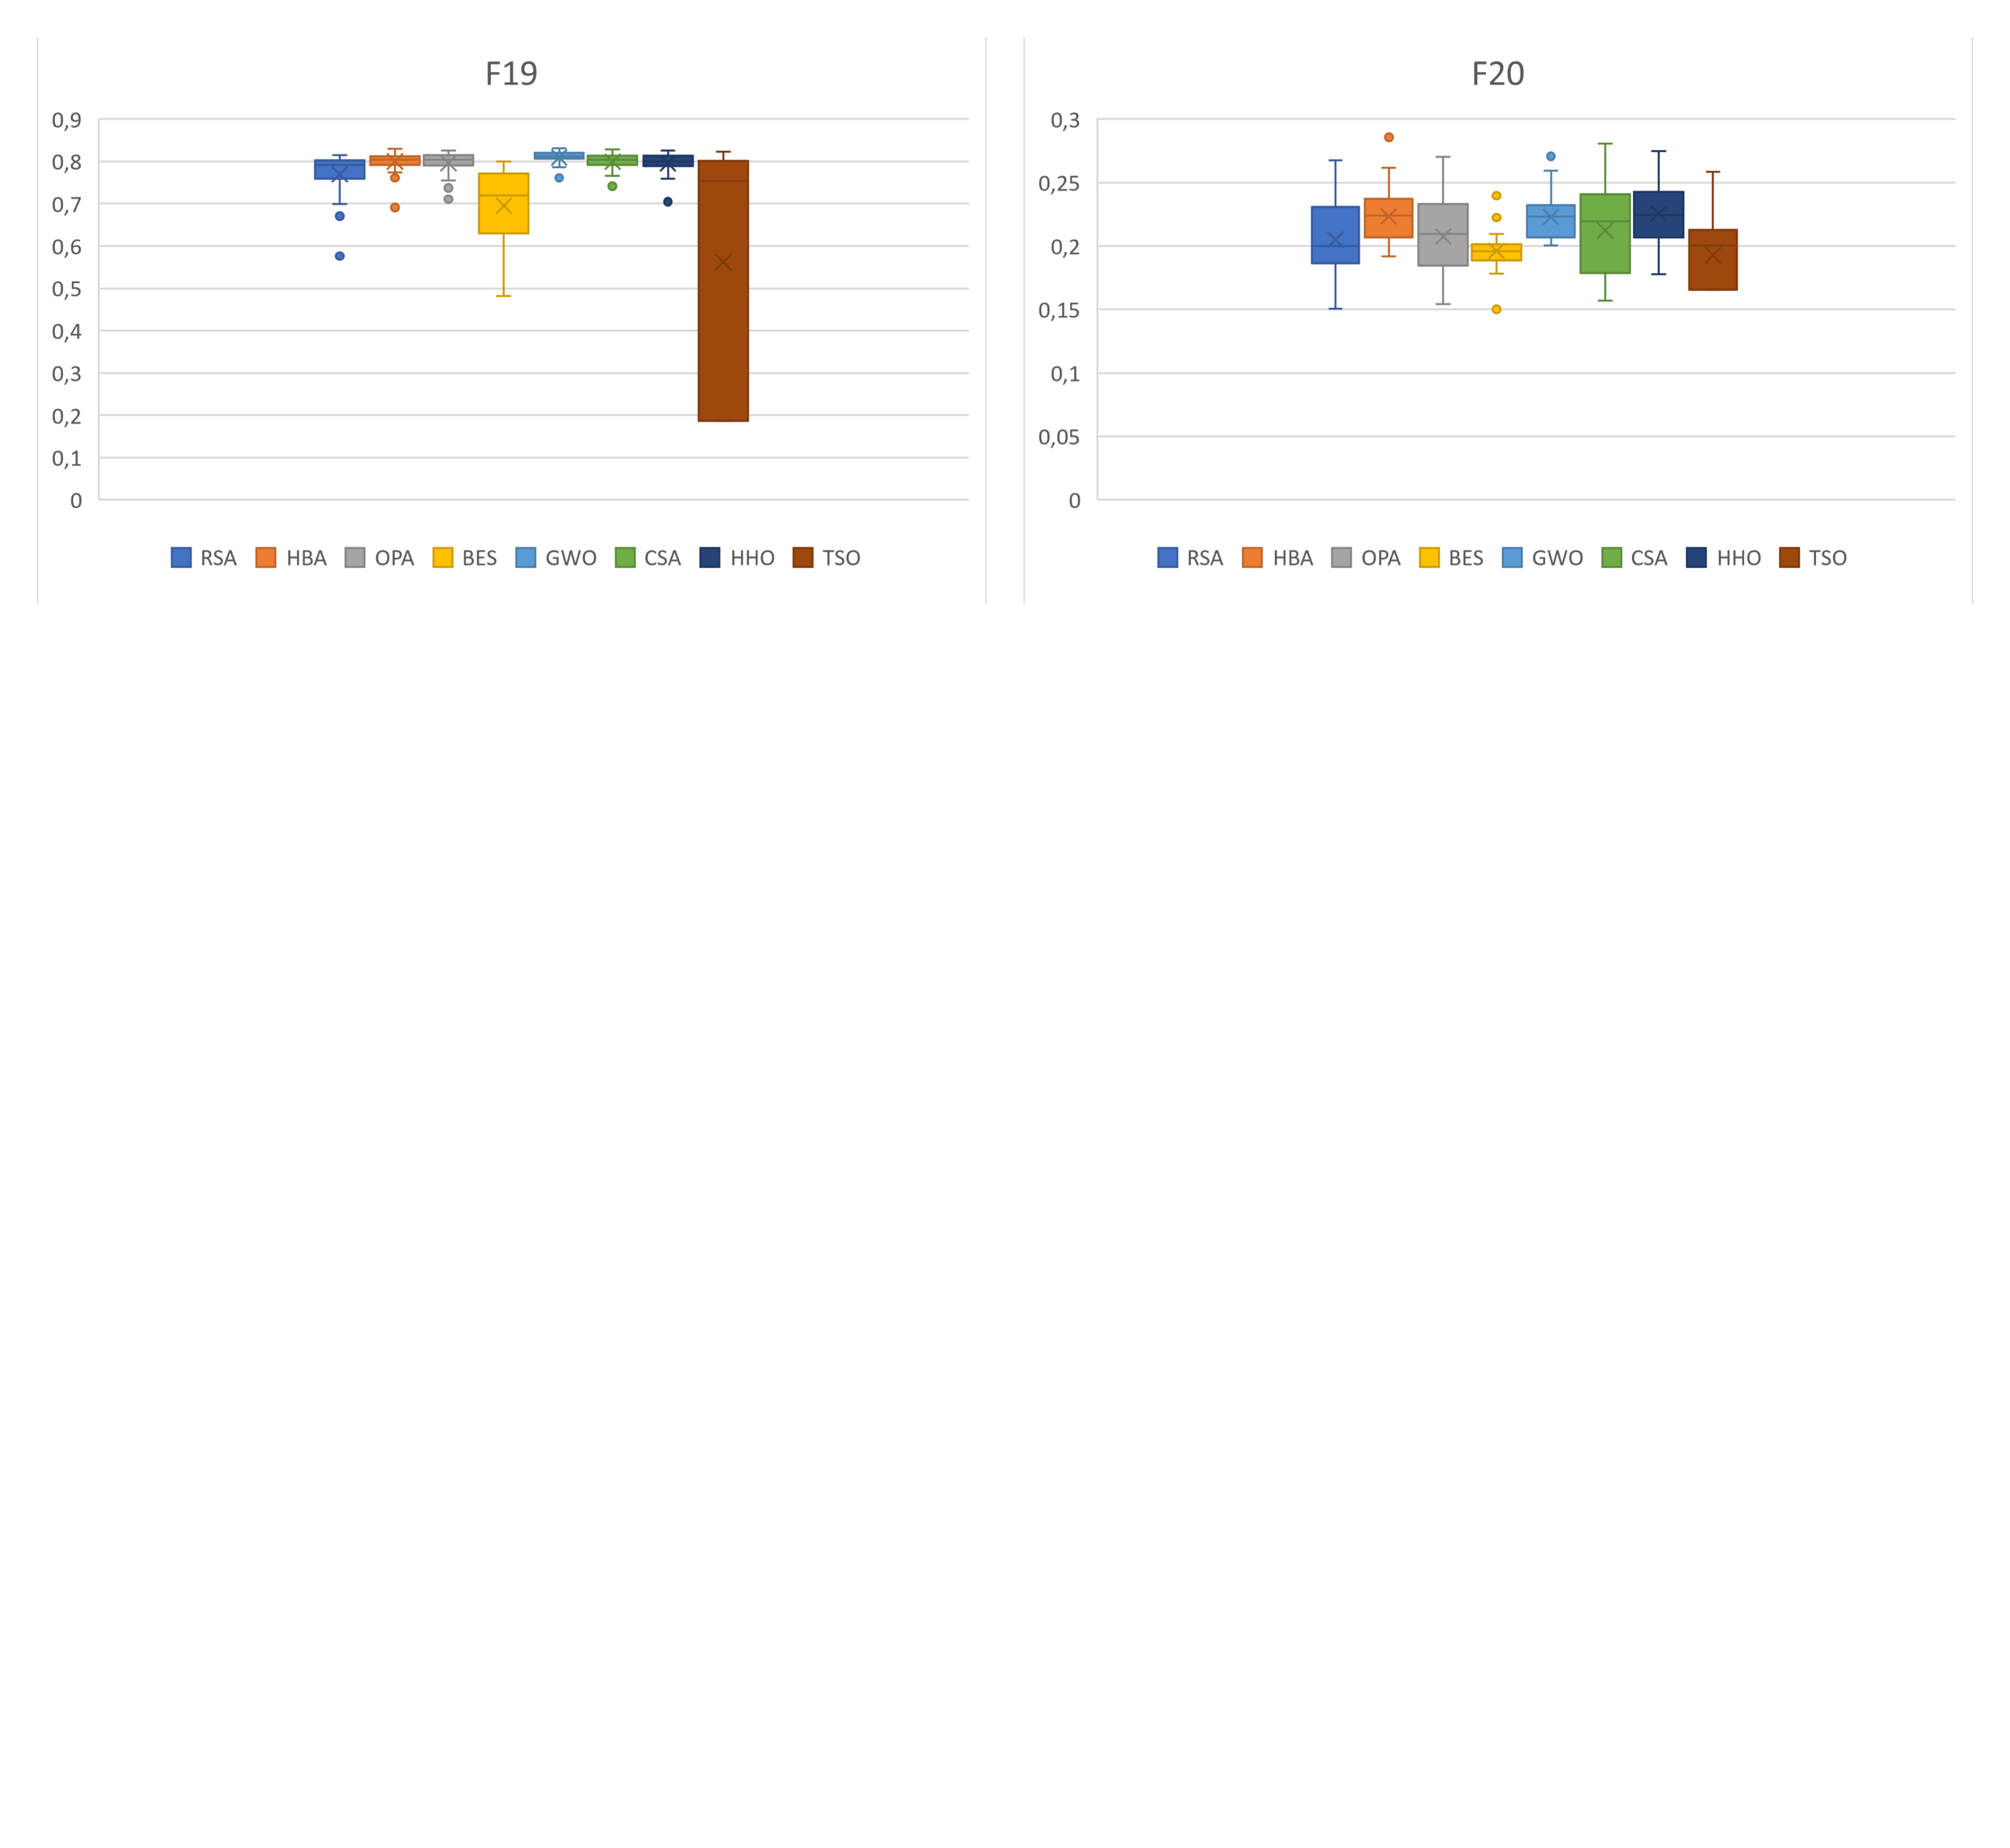
\includegraphics[width=\linewidth]{SSIM/Kapur/Dim7/SSIM_Dim7_Kapur_19_20.png}
		\vspace{-120pt} % Ajusta este valor según sea necesario
	\end{subfigure}
	\caption{Boxplot de los valores SSIM por cada imagen en la dimensión 7, desde la imagen 1 hasta la imagen 20,Función Entropía de Kapur}
	\label{fig:imagenes}    
\end{figure}

\subsubsection{Dimensión 8}
\begin{itemize}
\item RSA: Mostró un rendimiento medio a alto en las distintas métricas, con una variabilidad generalmente baja a moderada. Esto sugiere que es un algoritmo consistentemente confiable en la dimensión 8.

\item HBA: Exhibió un rendimiento similar al de RSA, con medianas consistentemente altas y un rango intercuartílico moderado. Parece ser un algoritmo estable con un buen rendimiento general.

\item OPA: Este algoritmo tuvo un rendimiento variable a lo largo de las métricas. Aunque en algunos casos mostró un rendimiento medio, también presentó cierta inconsistencia, como lo indican los valores atípicos y los rangos intercuartílicos más amplios.

\item BES: Generalmente, BES tuvo un rendimiento bajo, especialmente en las métricas F6 y F16, lo que lo identifica como uno de los algoritmos con menor rendimiento en la dimensión 8.

\item GWO: A pesar de tener valores atípicos en algunas métricas, GWO tuvo un buen rendimiento, particularmente destacando en la métrica F16 con una mediana alta, aunque con una variabilidad notable.

\item CSA: Este algoritmo mostró un rendimiento medio en la mayoría de las métricas, con una variabilidad moderada. No fue consistentemente el mejor ni el peor, colocándose en un término medio en términos de rendimiento y estabilidad.

\item HHO: Se mantuvo en el rango medio en términos de rendimiento, con una variabilidad relativamente baja a moderada. No se destacó particularmente ni hacia arriba ni hacia abajo en ninguna de las métricas.

\item TSO: Aunque tuvo el mejor rendimiento en la métrica F16, mostró gran variabilidad en otras métricas. Esta inconsistencia sugiere que, aunque puede ser capaz de alcanzar resultados altos, su rendimiento puede ser impredecible.
\end{itemize}
\noindent En resumen, si bien algunos algoritmos como GWO y TSO mostraron altos rendimientos en métricas individuales, RSA y HBA se destacaron por su consistencia y rendimiento general en la dimensión 8. En contraste, BES mostró un área de preocupación debido a su bajo rendimiento. La elección del algoritmo adecuado dependerá del equilibrio entre el rendimiento medio y la consistencia de los resultados según sea prioritario para la aplicación o la investigación en cuestión.
%% Boxplot de los valores SSIM por cada imagen en la dimensión 8, desde la imagen 1 hasta la imagen 20,Función Entropía de Kapur
\begin{figure}
	\centering
	
	\begin{subfigure}{0.4\textwidth}
		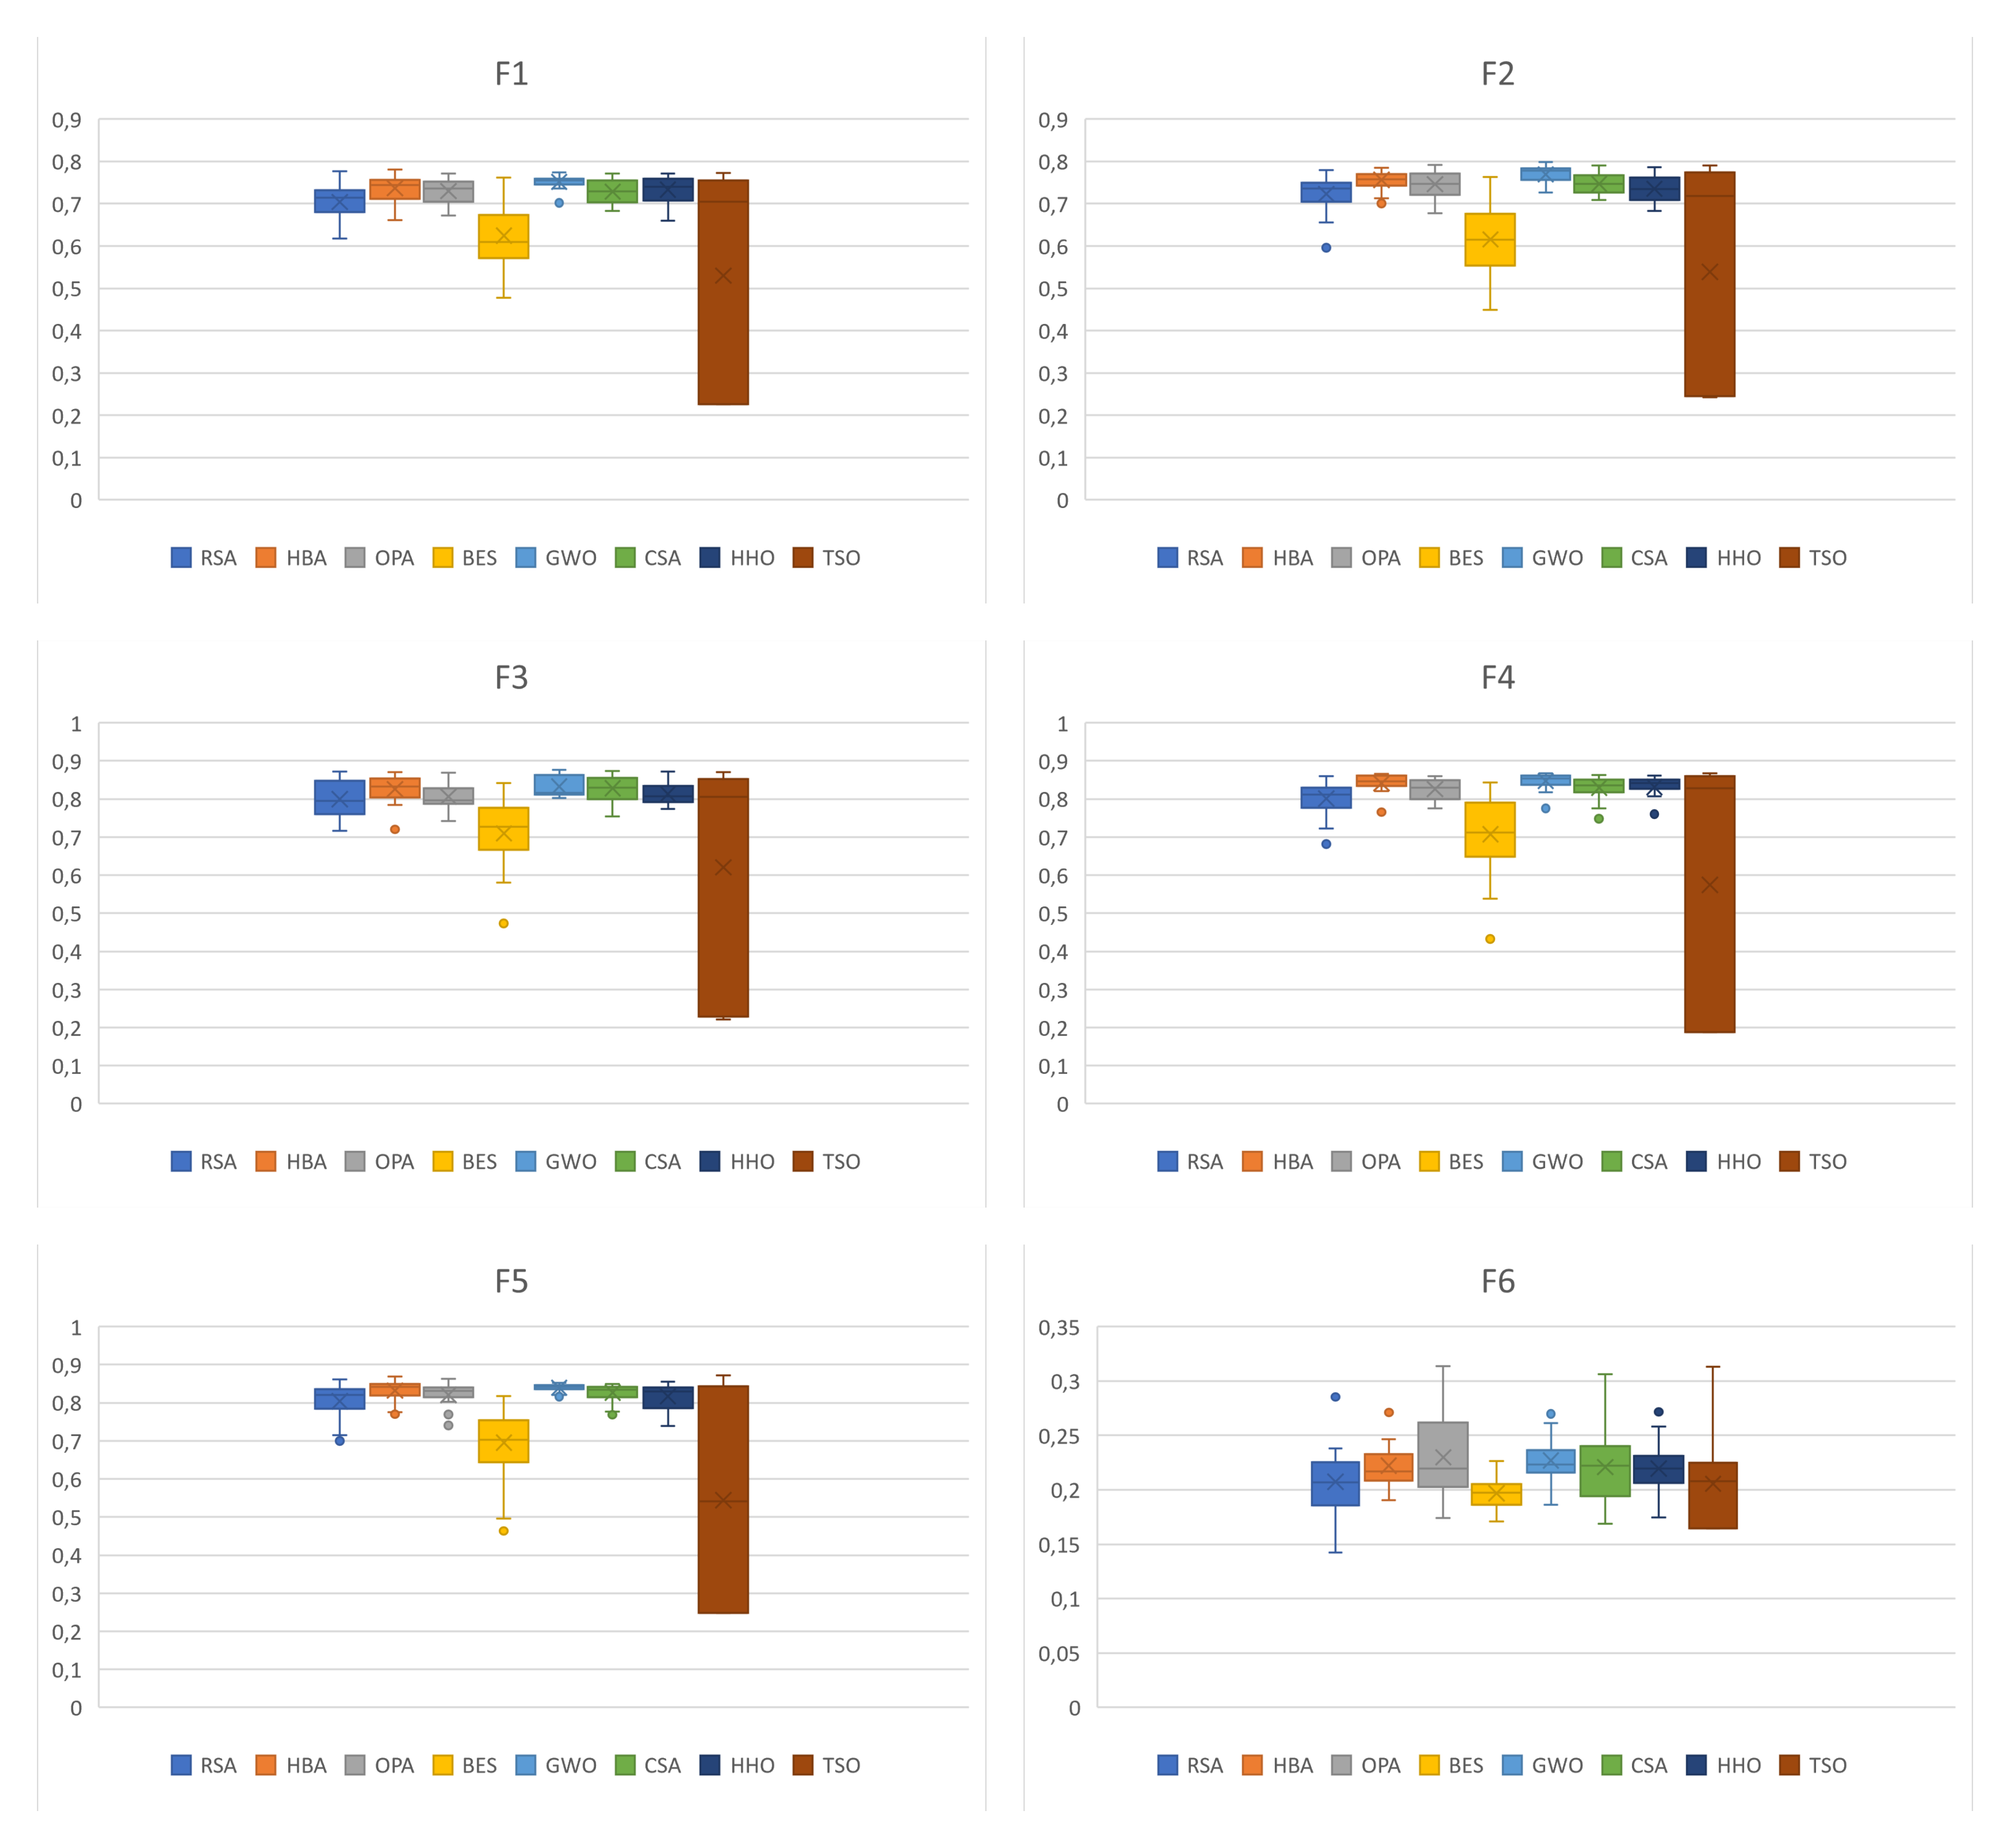
\includegraphics[width=\linewidth]{SSIM/Kapur/Dim8/SSIM_Dim8_Kapur_1_6.png}
	\end{subfigure}
	
	\begin{subfigure}{0.4\textwidth}
		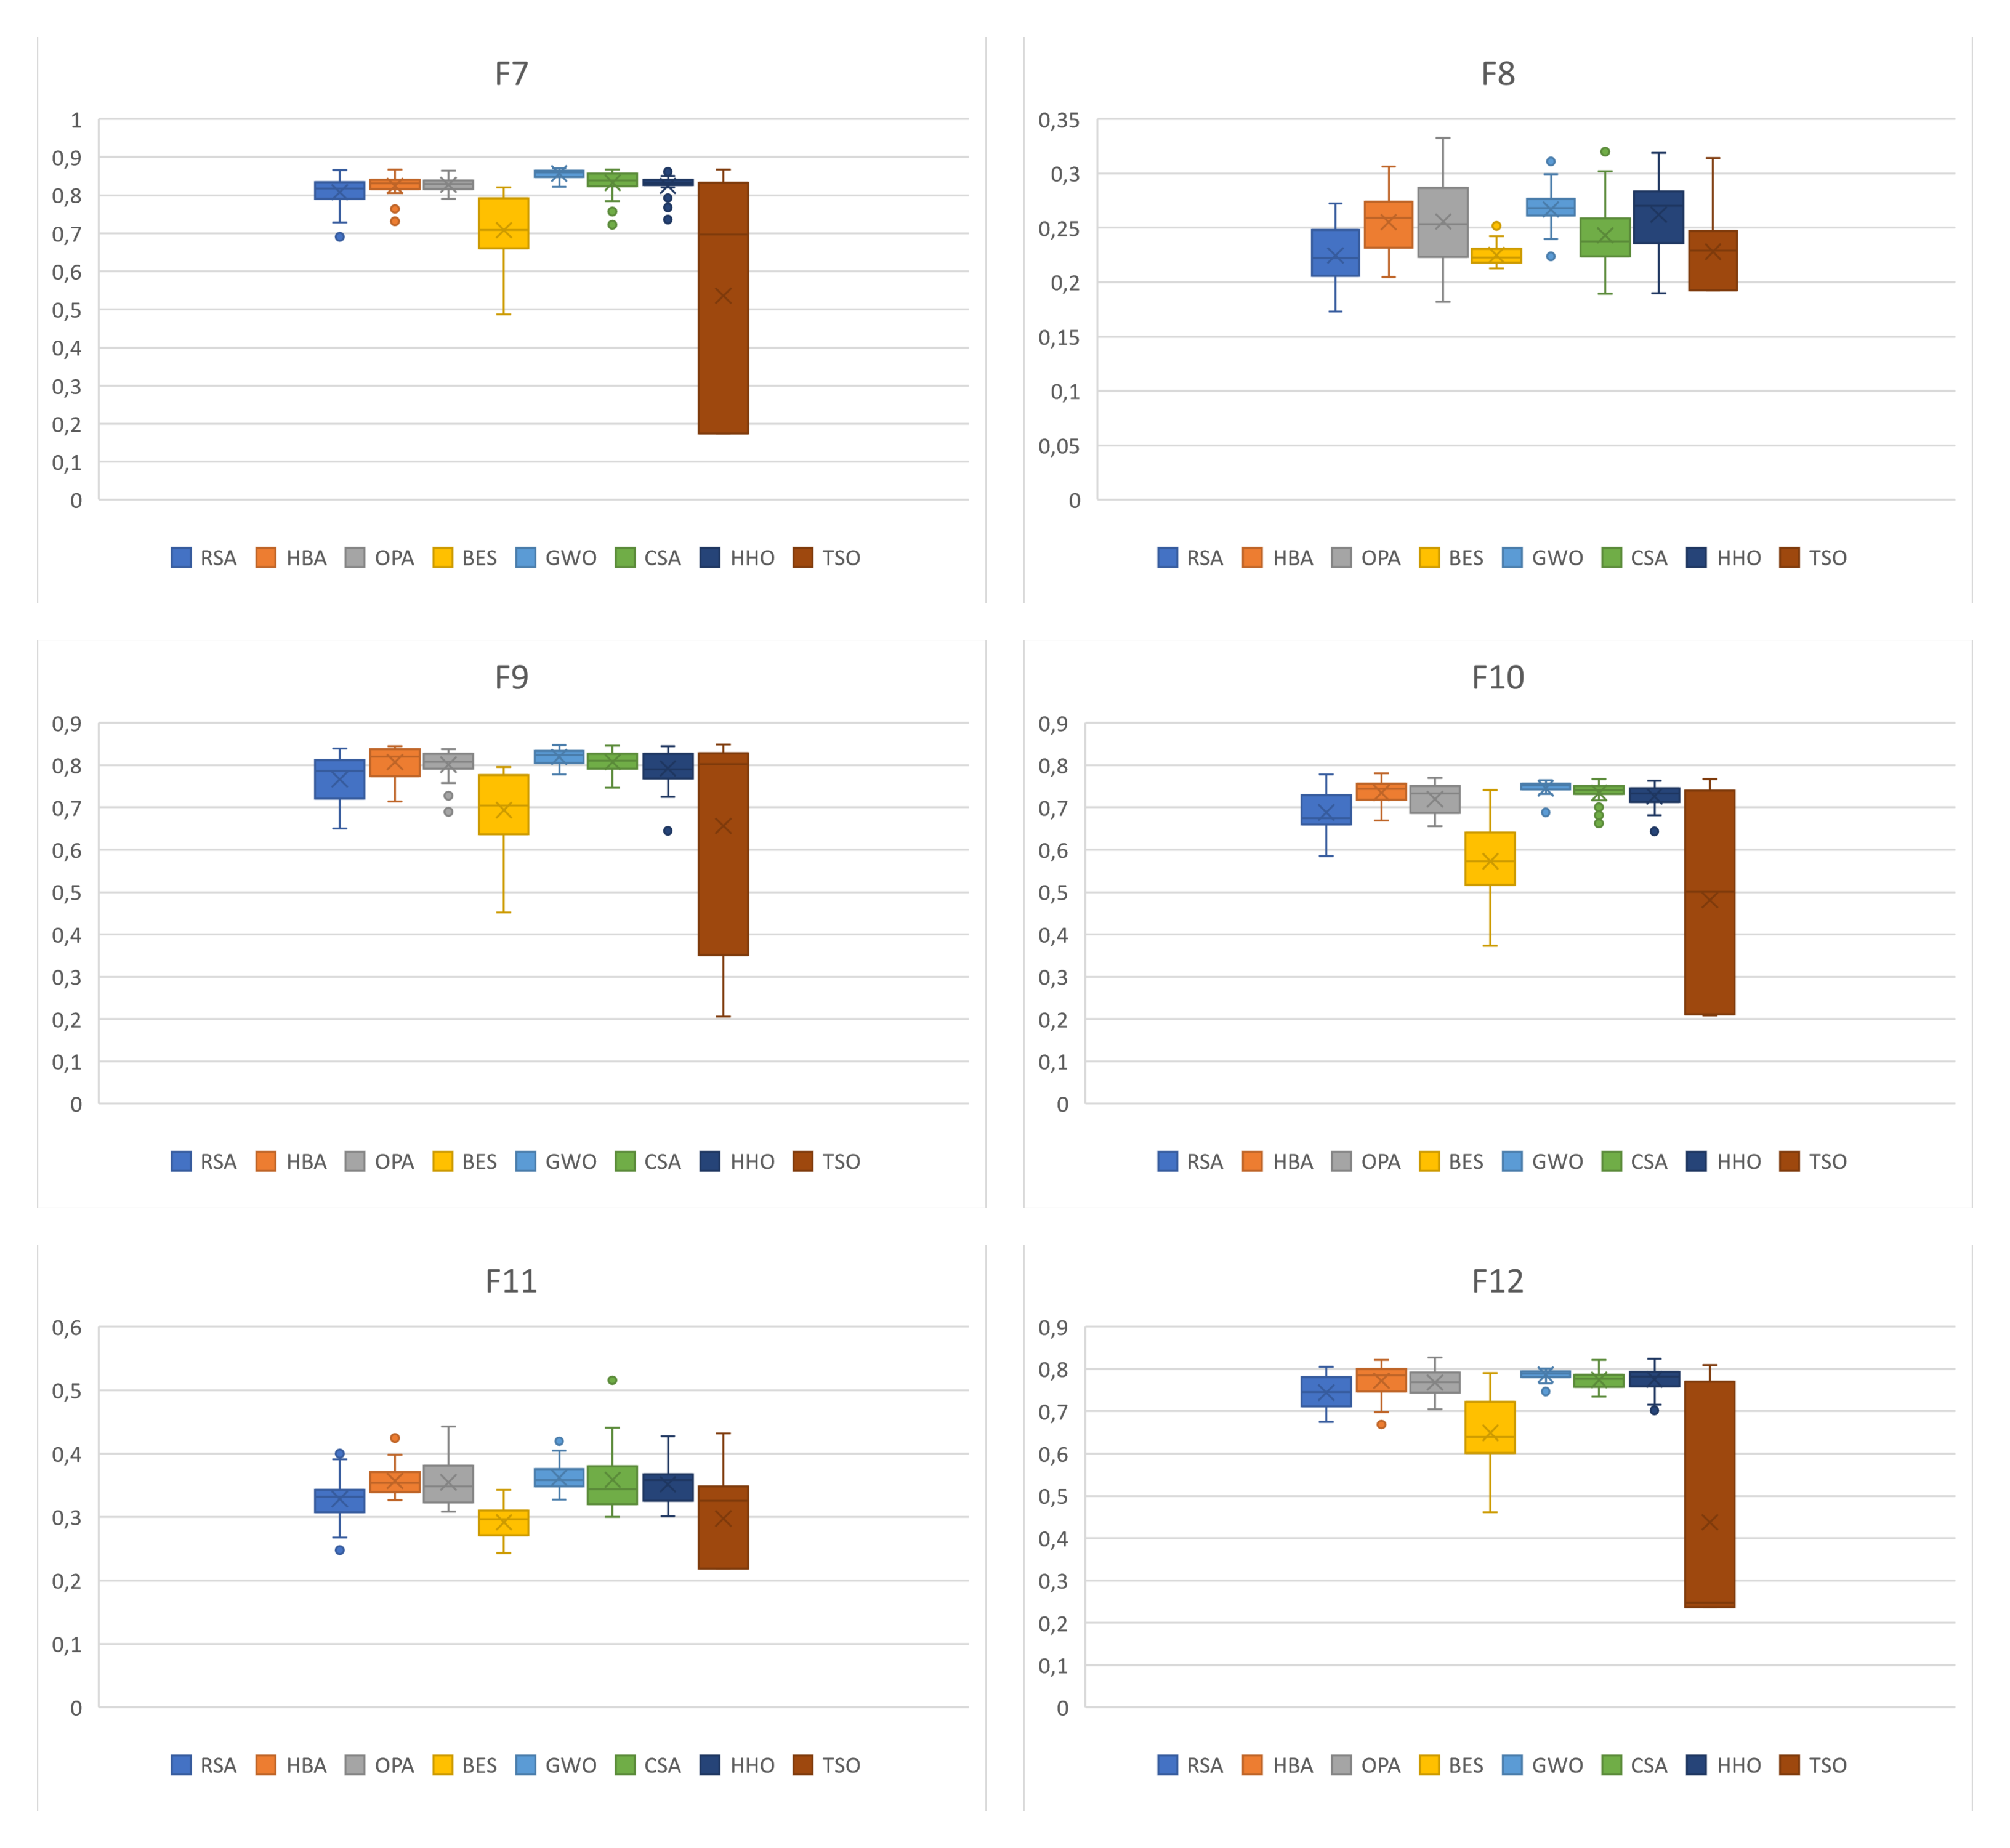
\includegraphics[width=\linewidth]{SSIM/Kapur/Dim8/SSIM_Dim8_Kapur_7_12.png}
	\end{subfigure}  
	\begin{subfigure}{0.4\textwidth}
		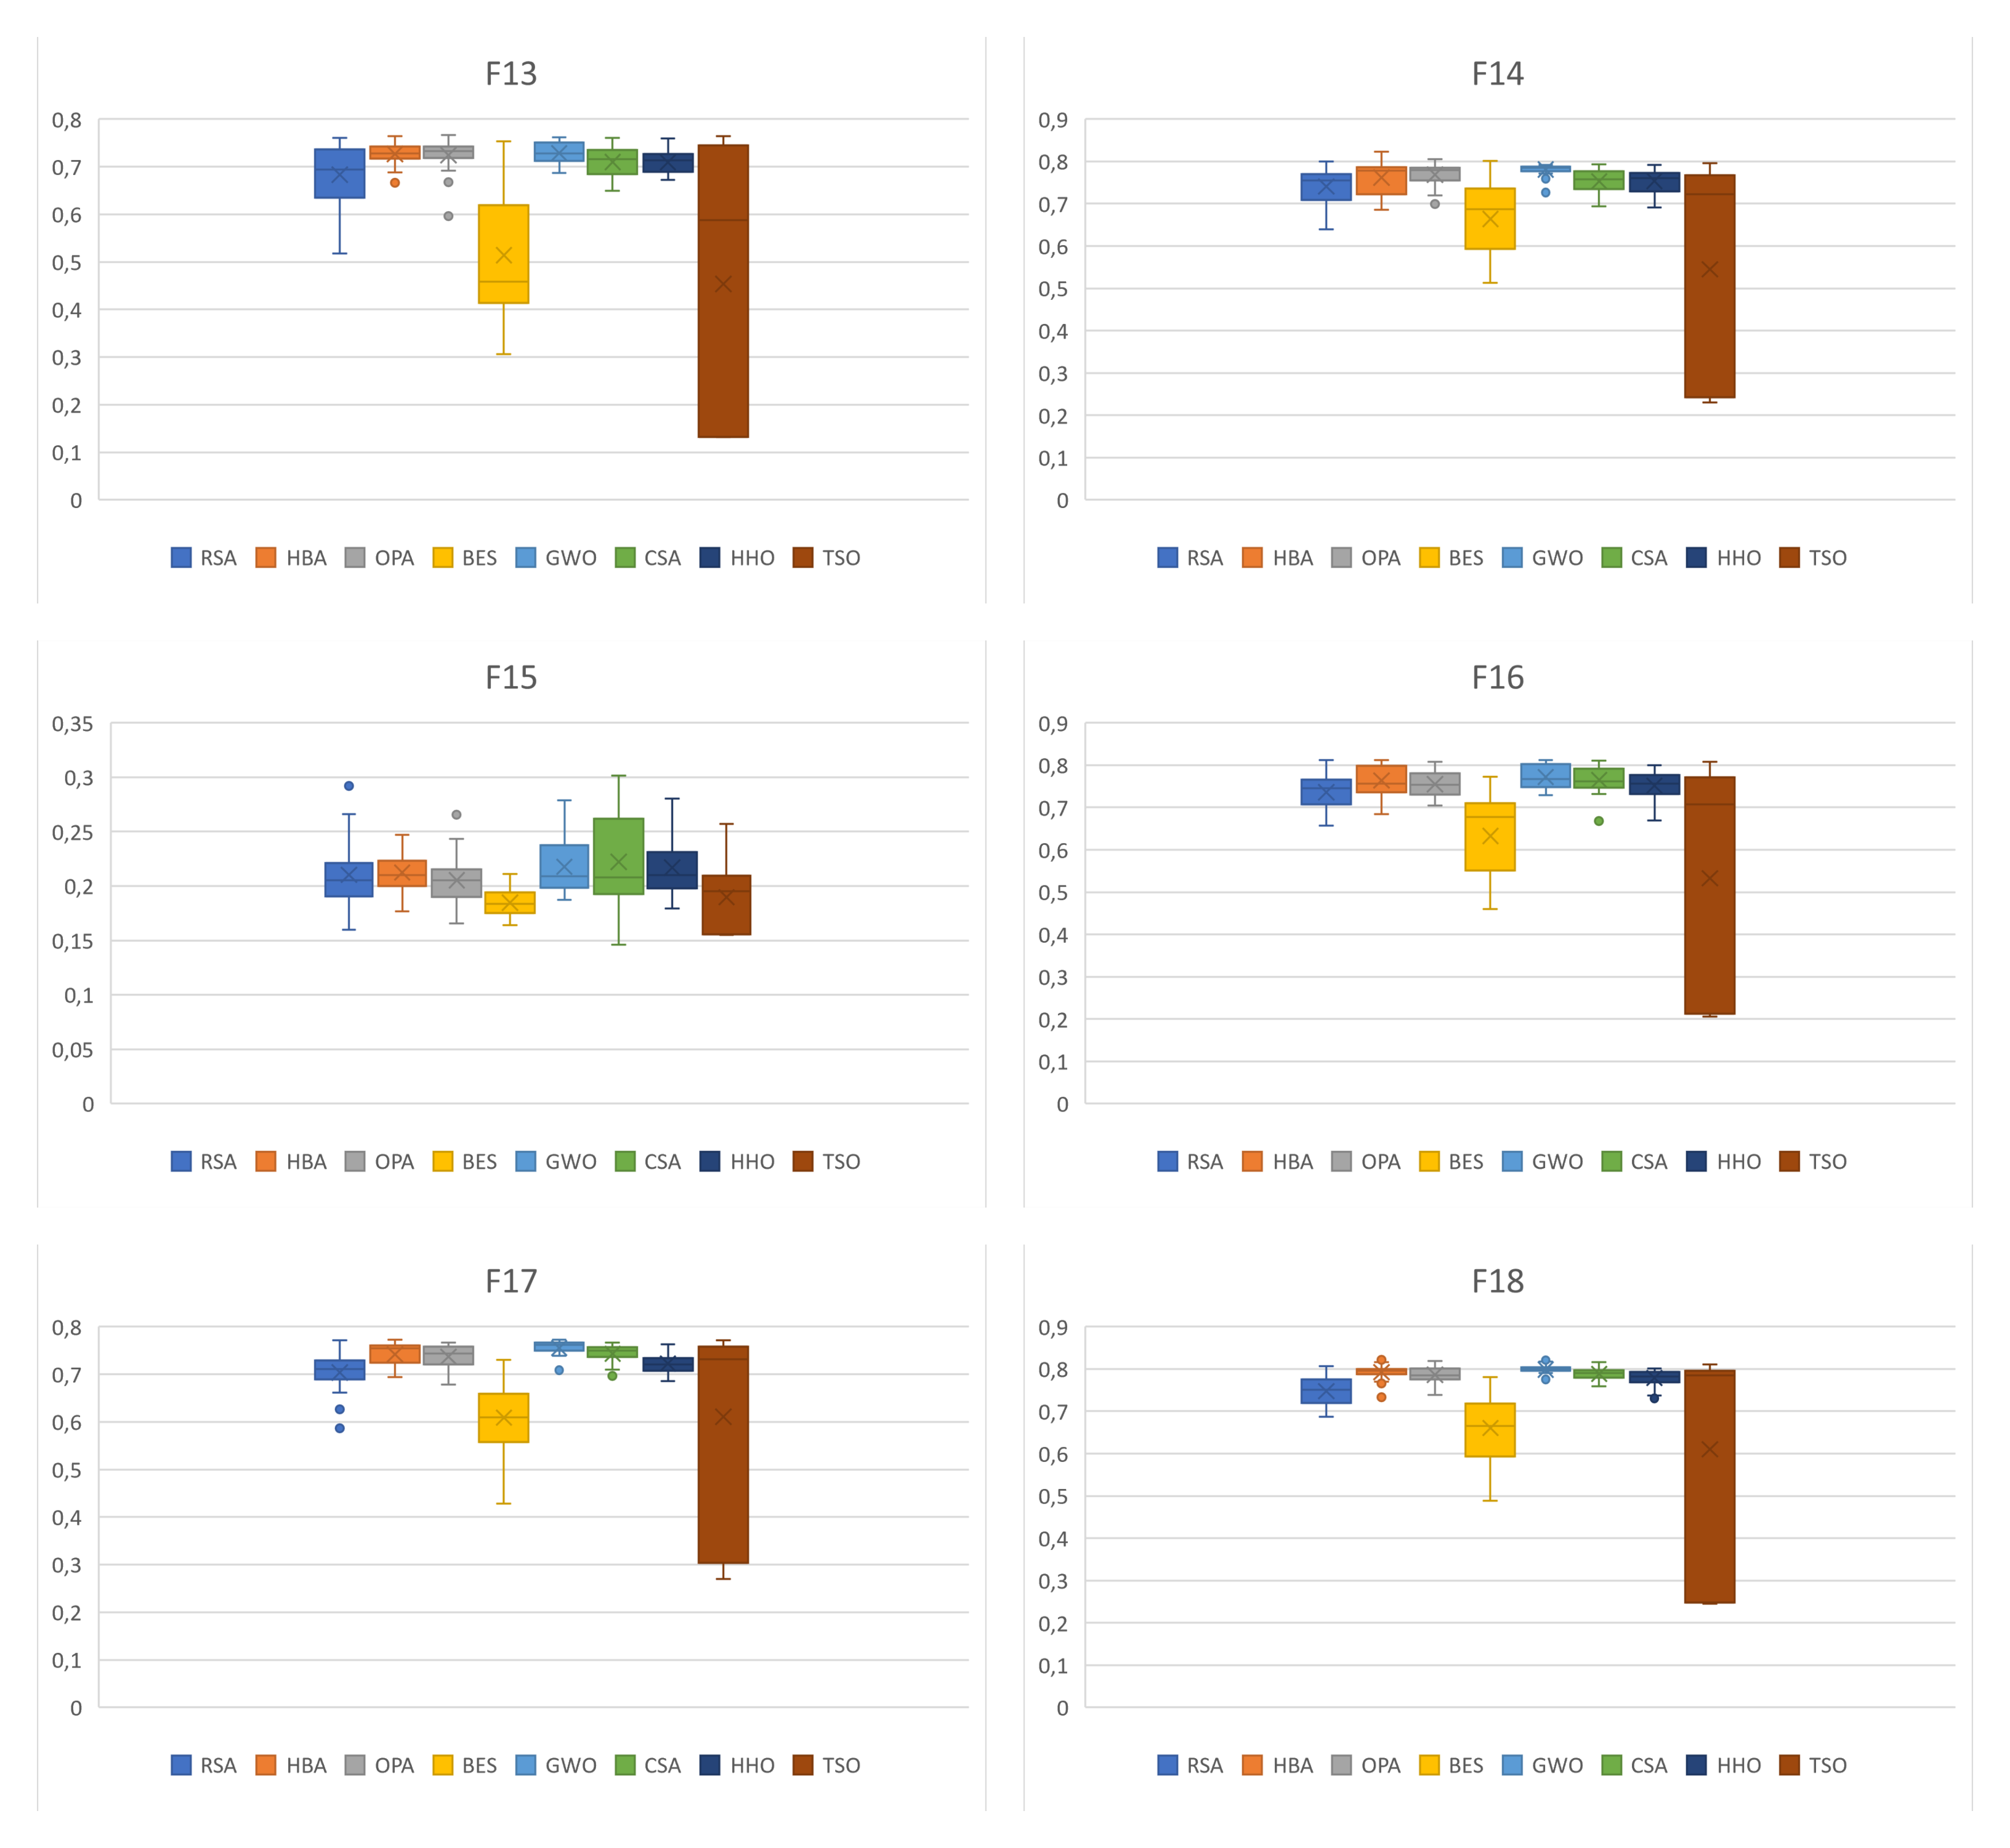
\includegraphics[width=\linewidth]{SSIM/Kapur/Dim8/SSIM_Dim8_Kapur_13_18.png}
		%\vspace{-150pt} % Ajusta este valor según sea necesario
	\end{subfigure}   
	\begin{subfigure}{0.4\textwidth}
		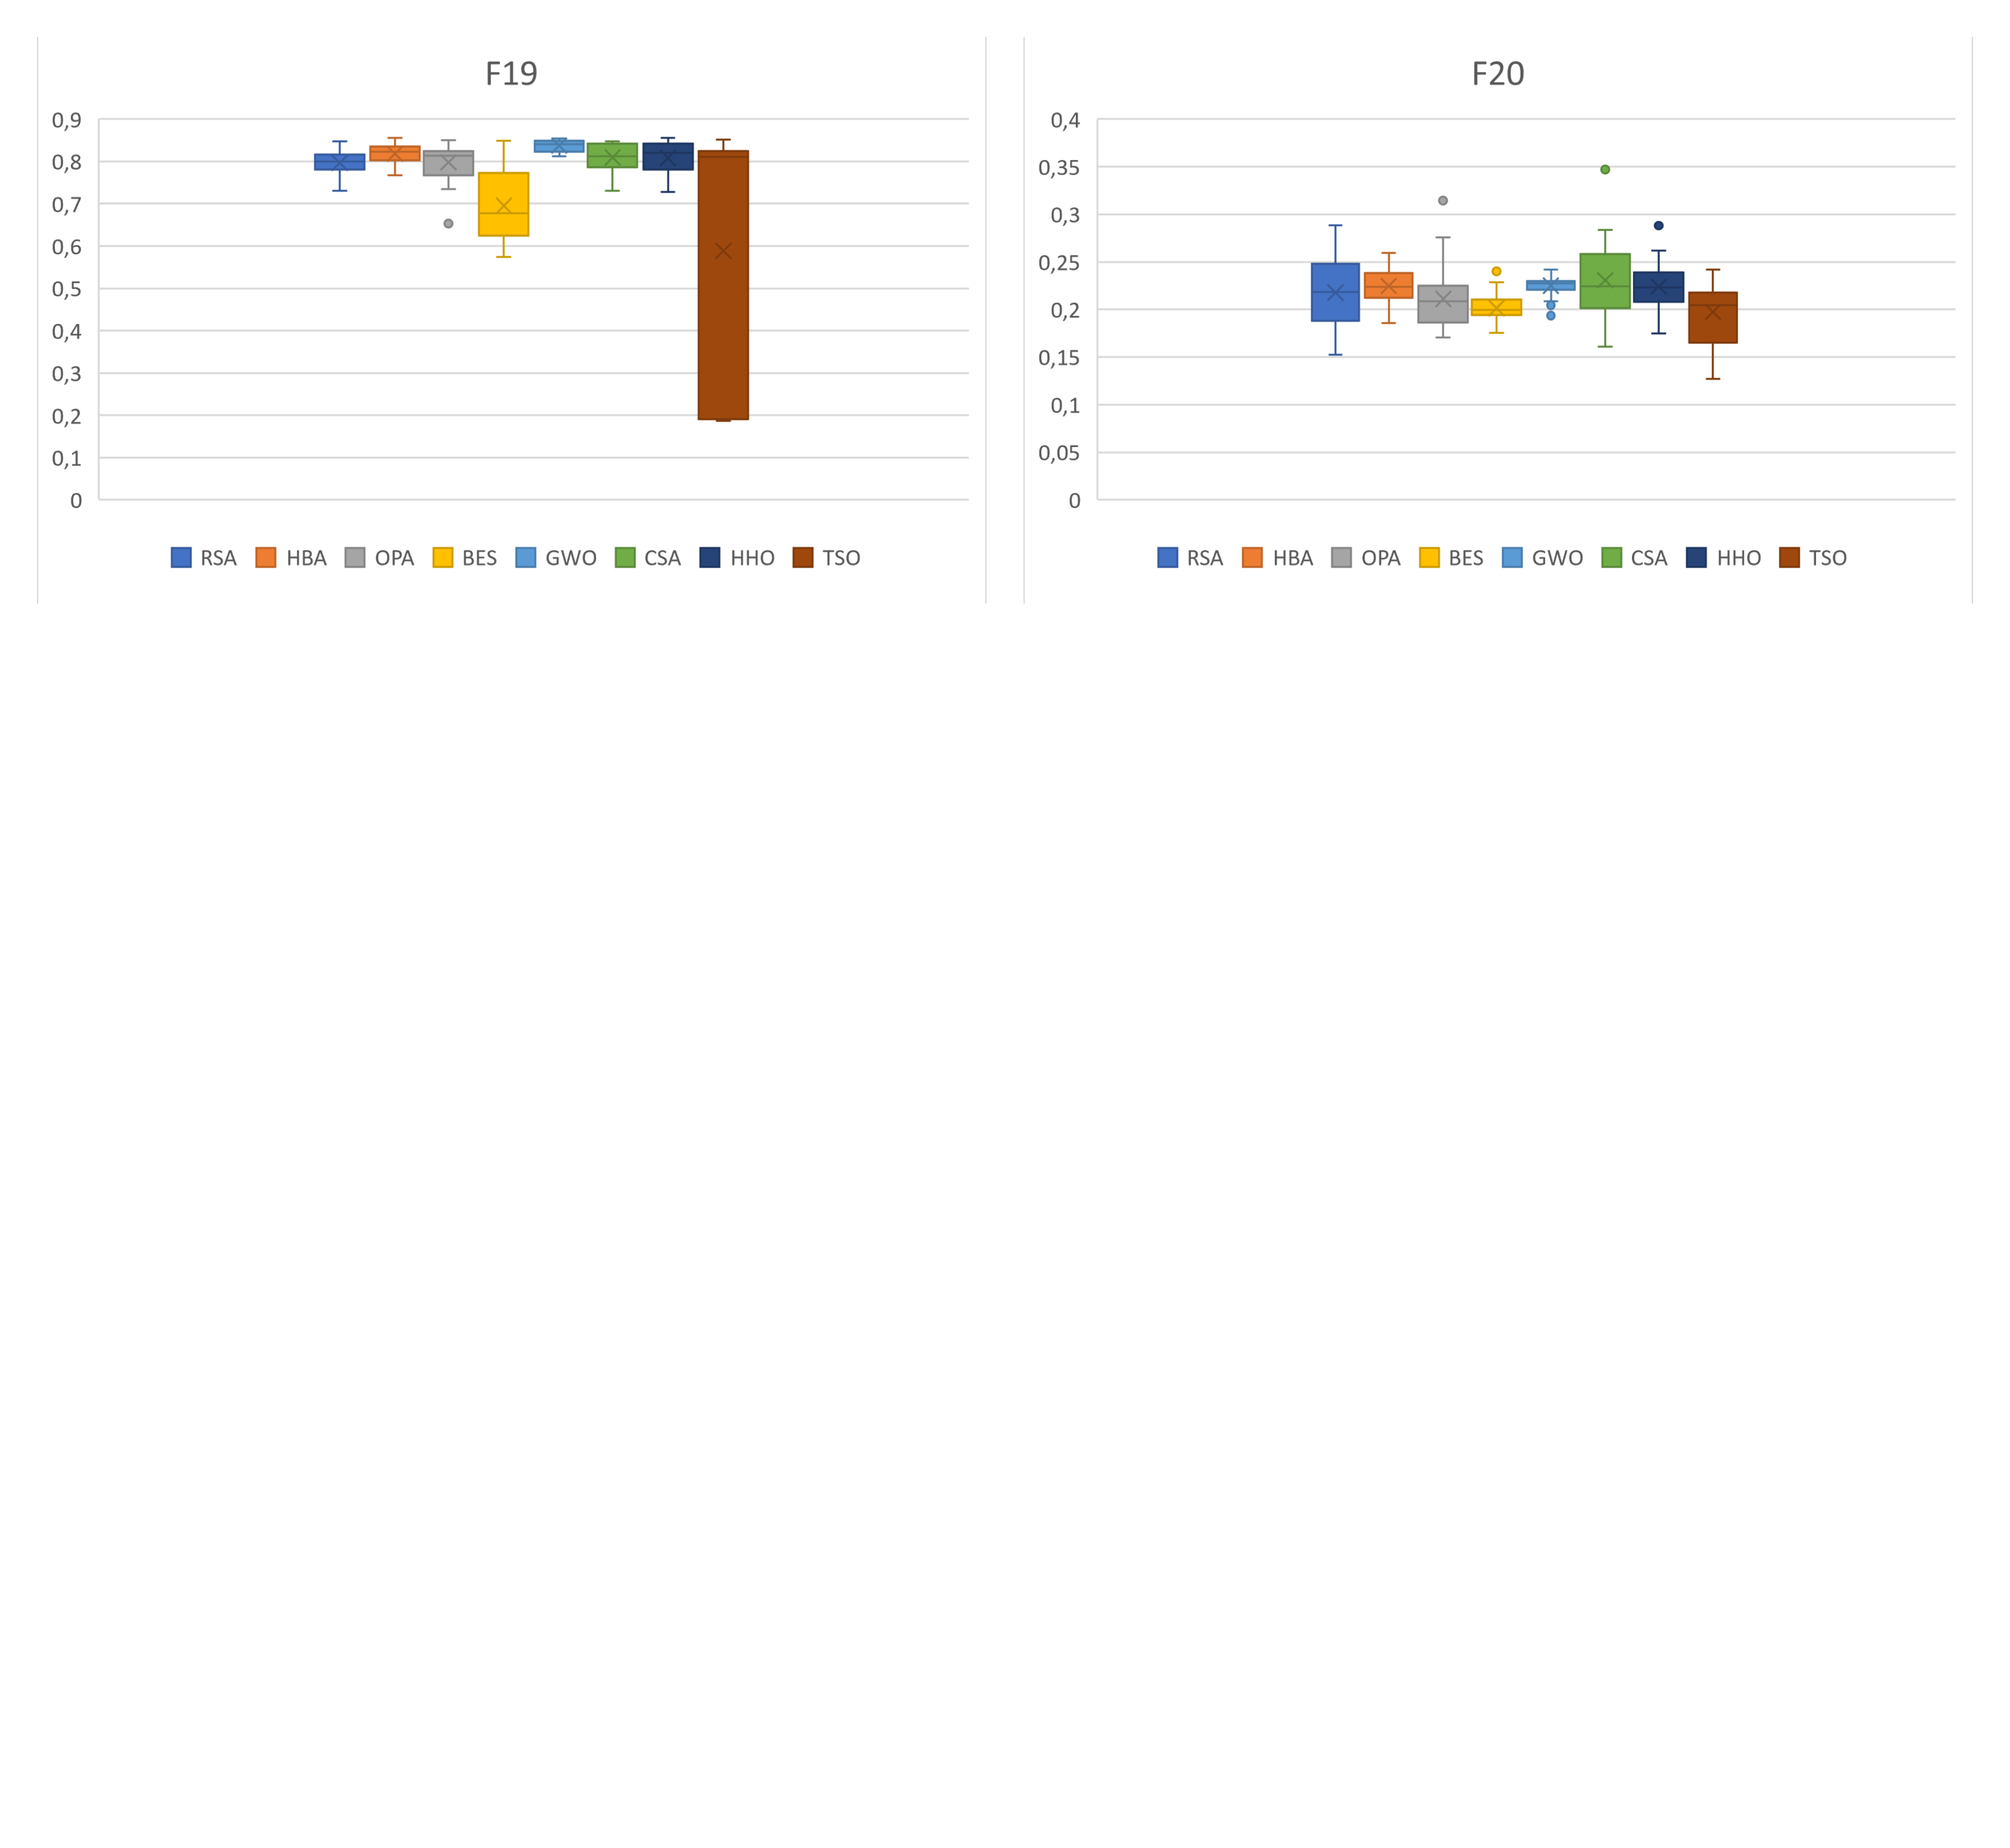
\includegraphics[width=\linewidth]{SSIM/Kapur/Dim8/SSIM_Dim8_Kapur_19_20.png}
		\vspace{-120pt} % Ajusta este valor según sea necesario
	\end{subfigure}
	\caption{Boxplot de los valores SSIM por cada imagen en la dimensión 8, desde la imagen 1 hasta la imagen 20,Función Entropía de Kapur}
	\label{fig:imagenes}    
\end{figure}
\subsubsection{Dimensión 9}
\begin{itemize}
\item RSA: Muestra una consistencia relativamente buena en todas las métricas, con medianas en el rango medio y variabilidad moderada. No sobresale particularmente en ninguna de las métricas, pero tampoco está en el extremo inferior.

\item HBA: Similar a RSA, HBA tiene un rendimiento medio con variabilidad moderada en todas las métricas. No muestra extremos en términos de rendimiento, lo cual podría hacerlo un algoritmo confiable en términos de predecibilidad.

\item OPA: Este algoritmo tiene un rango intercuartílico más amplio en algunas métricas, indicando una mayor variabilidad. Aunque su rendimiento no es el más bajo, la inconsistencia en los resultados podría ser una preocupación.

\item BES: Consistentemente tiene un rendimiento inferior en todas las métricas examinadas, con las medianas más bajas. Esto indica que BES podría no ser adecuado para aplicaciones en la dimensión 9 que requieren un alto rendimiento en estas métricas.

\item GWO: Tiene un buen rendimiento en general, particularmente en las métricas F11 y F16, aunque presenta algunos valores atípicos. La variabilidad es moderada, lo que sugiere que es un algoritmo bastante robusto en esta dimensión.

\item CSA: Muestra un rendimiento medio a bueno con variabilidad moderada en todas las métricas. No es el mejor en ninguna de las métricas, pero su rendimiento es generalmente estable.

\item HHO: Presenta resultados consistentes y medianas que indican un rendimiento medio. Similar a CSA, no tiene el mejor ni el peor rendimiento, manteniéndose en un rango medio en todas las métricas.

\item TSO: A pesar de tener la mediana más alta en la métrica F16, su rendimiento es altamente variable, como lo indican los rangos intercuartílicos grandes en varias métricas. Esto sugiere que, aunque tiene el potencial de alcanzar un alto rendimiento, su comportamiento puede ser impredecible.

\end{itemize}
\noindent En resumen, mientras que BES parece ser el menos adecuado en la dimensión 9 en base a estas métricas, GWO y CSA muestran un buen equilibrio de rendimiento y consistencia. TSO, aunque a veces alcanza altos valores, su variabilidad puede ser problemática. RSA, HBA, y HHO parecen ser opciones intermedias en términos de rendimiento y estabilidad.

%% Boxplot de los valores SSIM por cada imagen en la dimensión 9, desde la imagen 11 hasta la imagen 20,Función Entropía de Kapur
\begin{figure}
	\centering
	
	\begin{subfigure}{0.4\textwidth}
		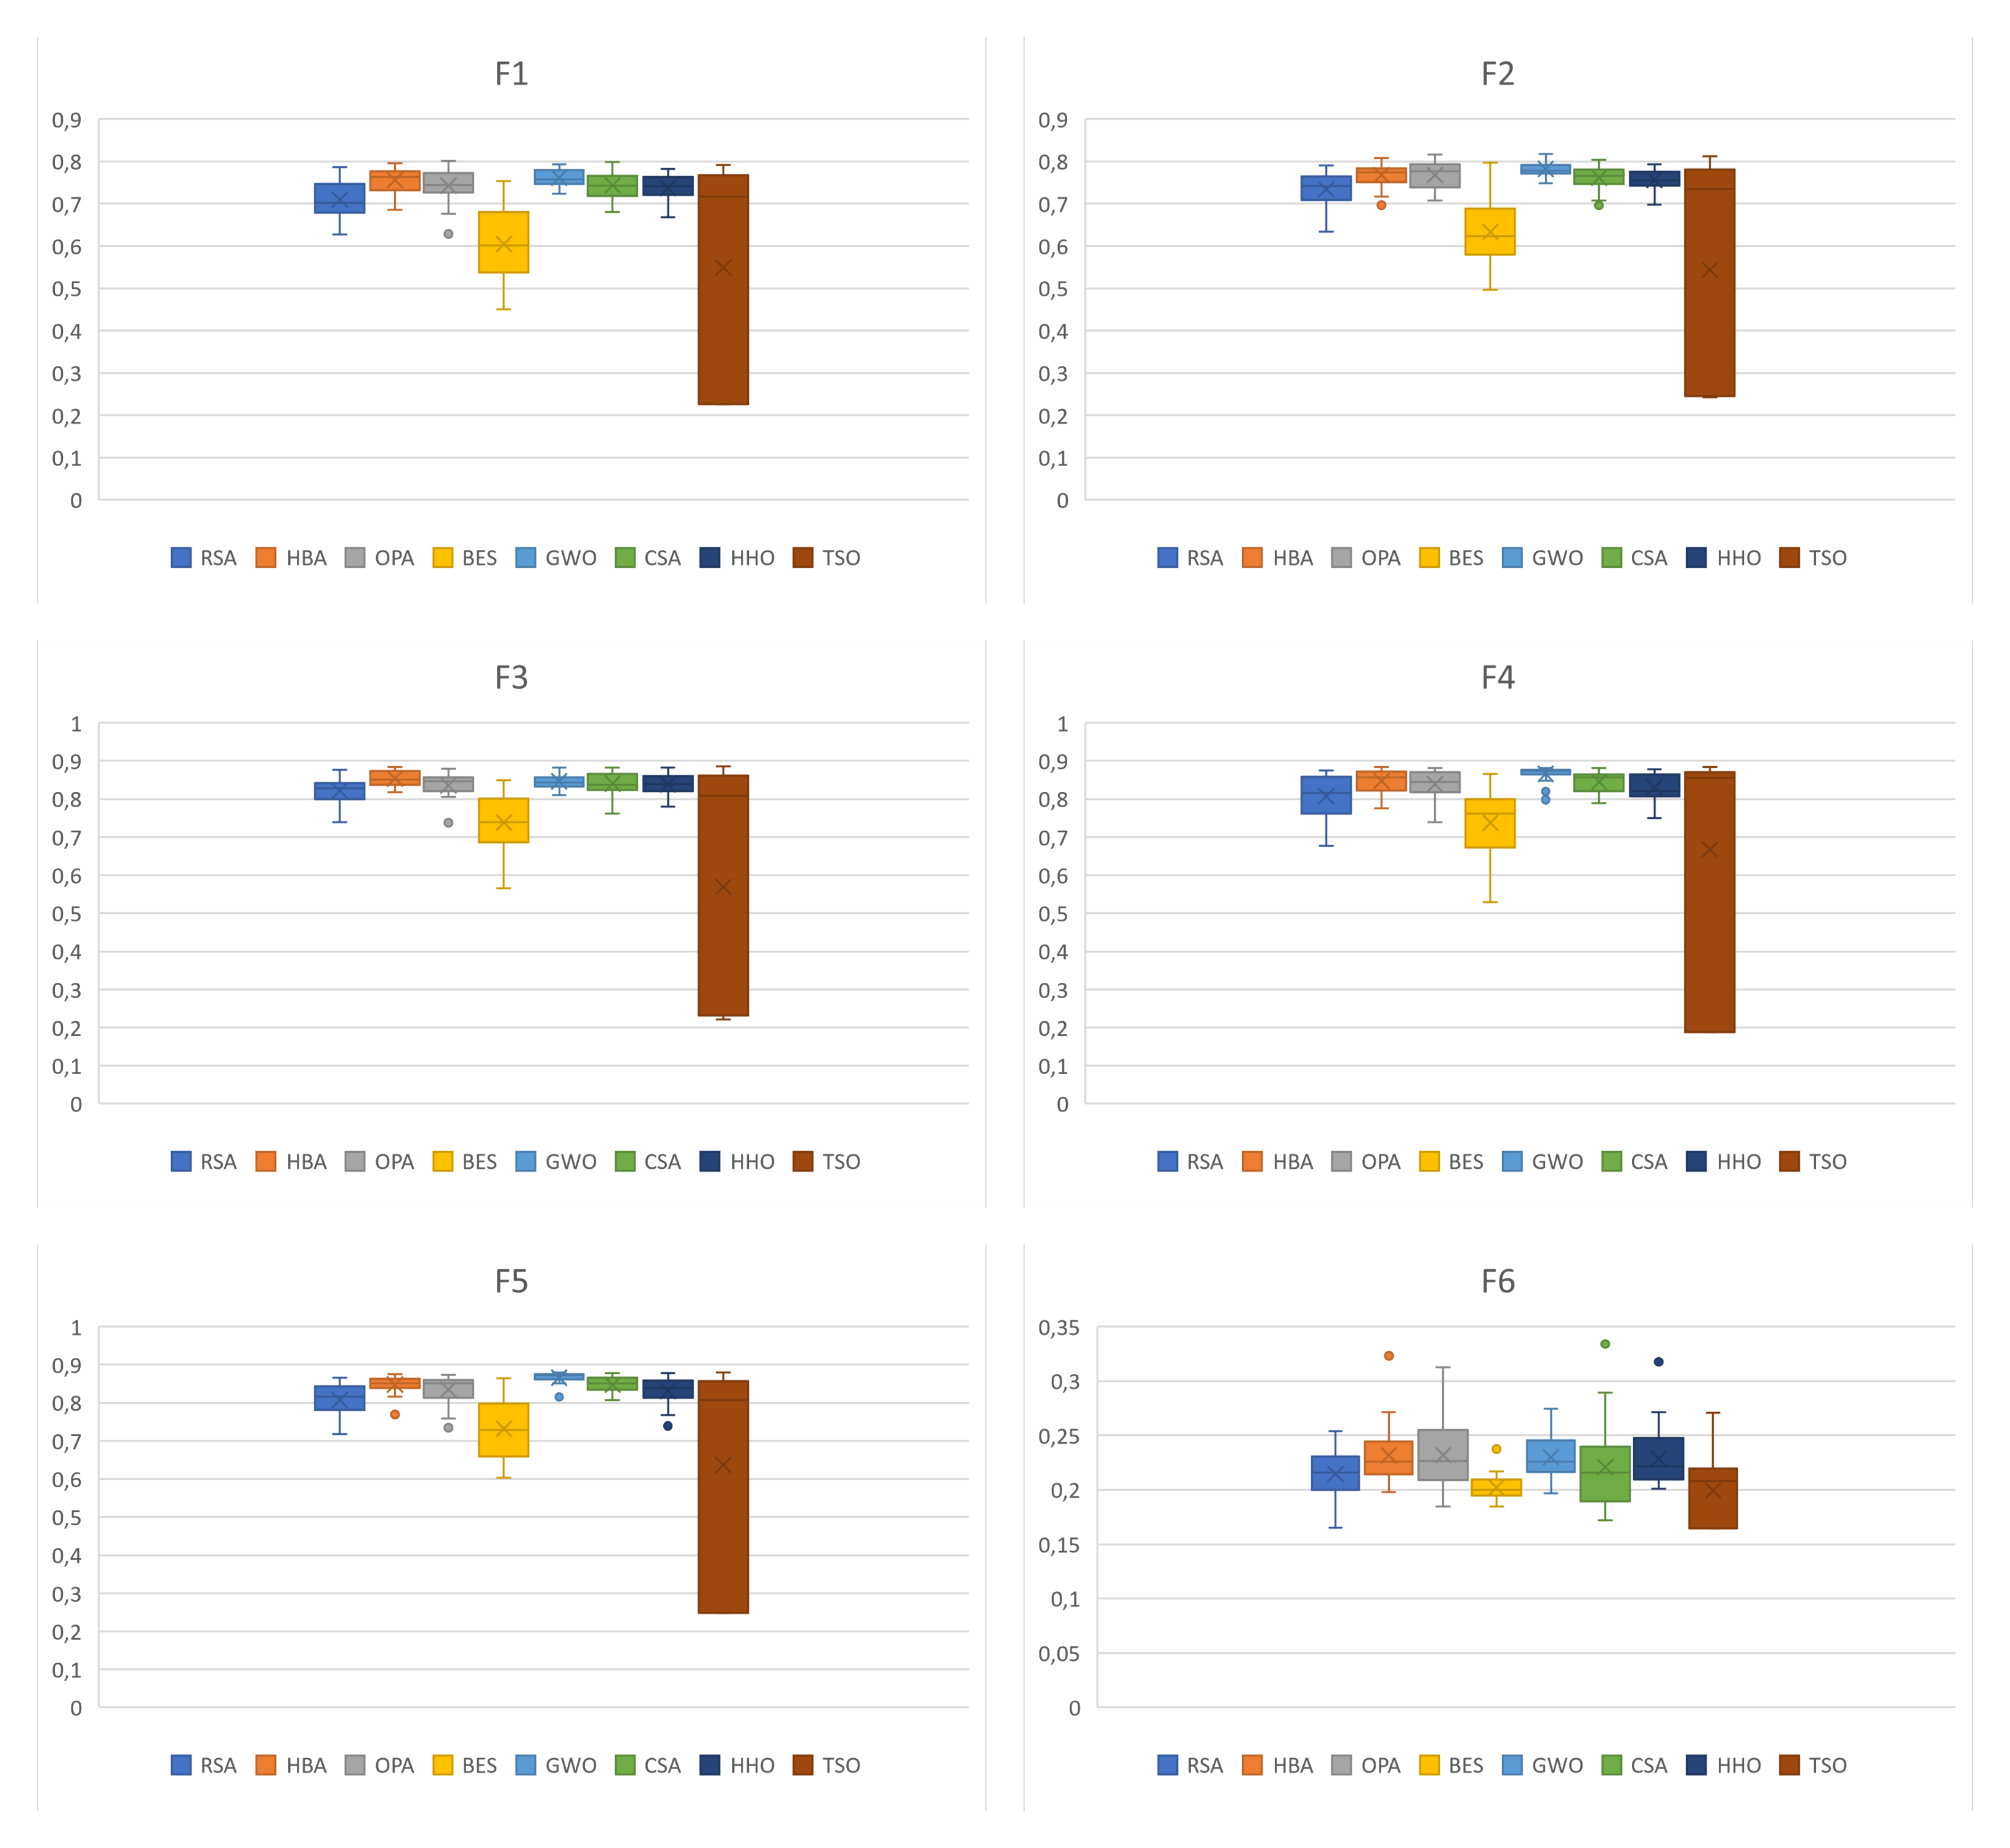
\includegraphics[width=\linewidth]{SSIM/Kapur/Dim9/SSIM_Dim9_Kapur_1_6.png}
	\end{subfigure}
	
	\begin{subfigure}{0.4\textwidth}
		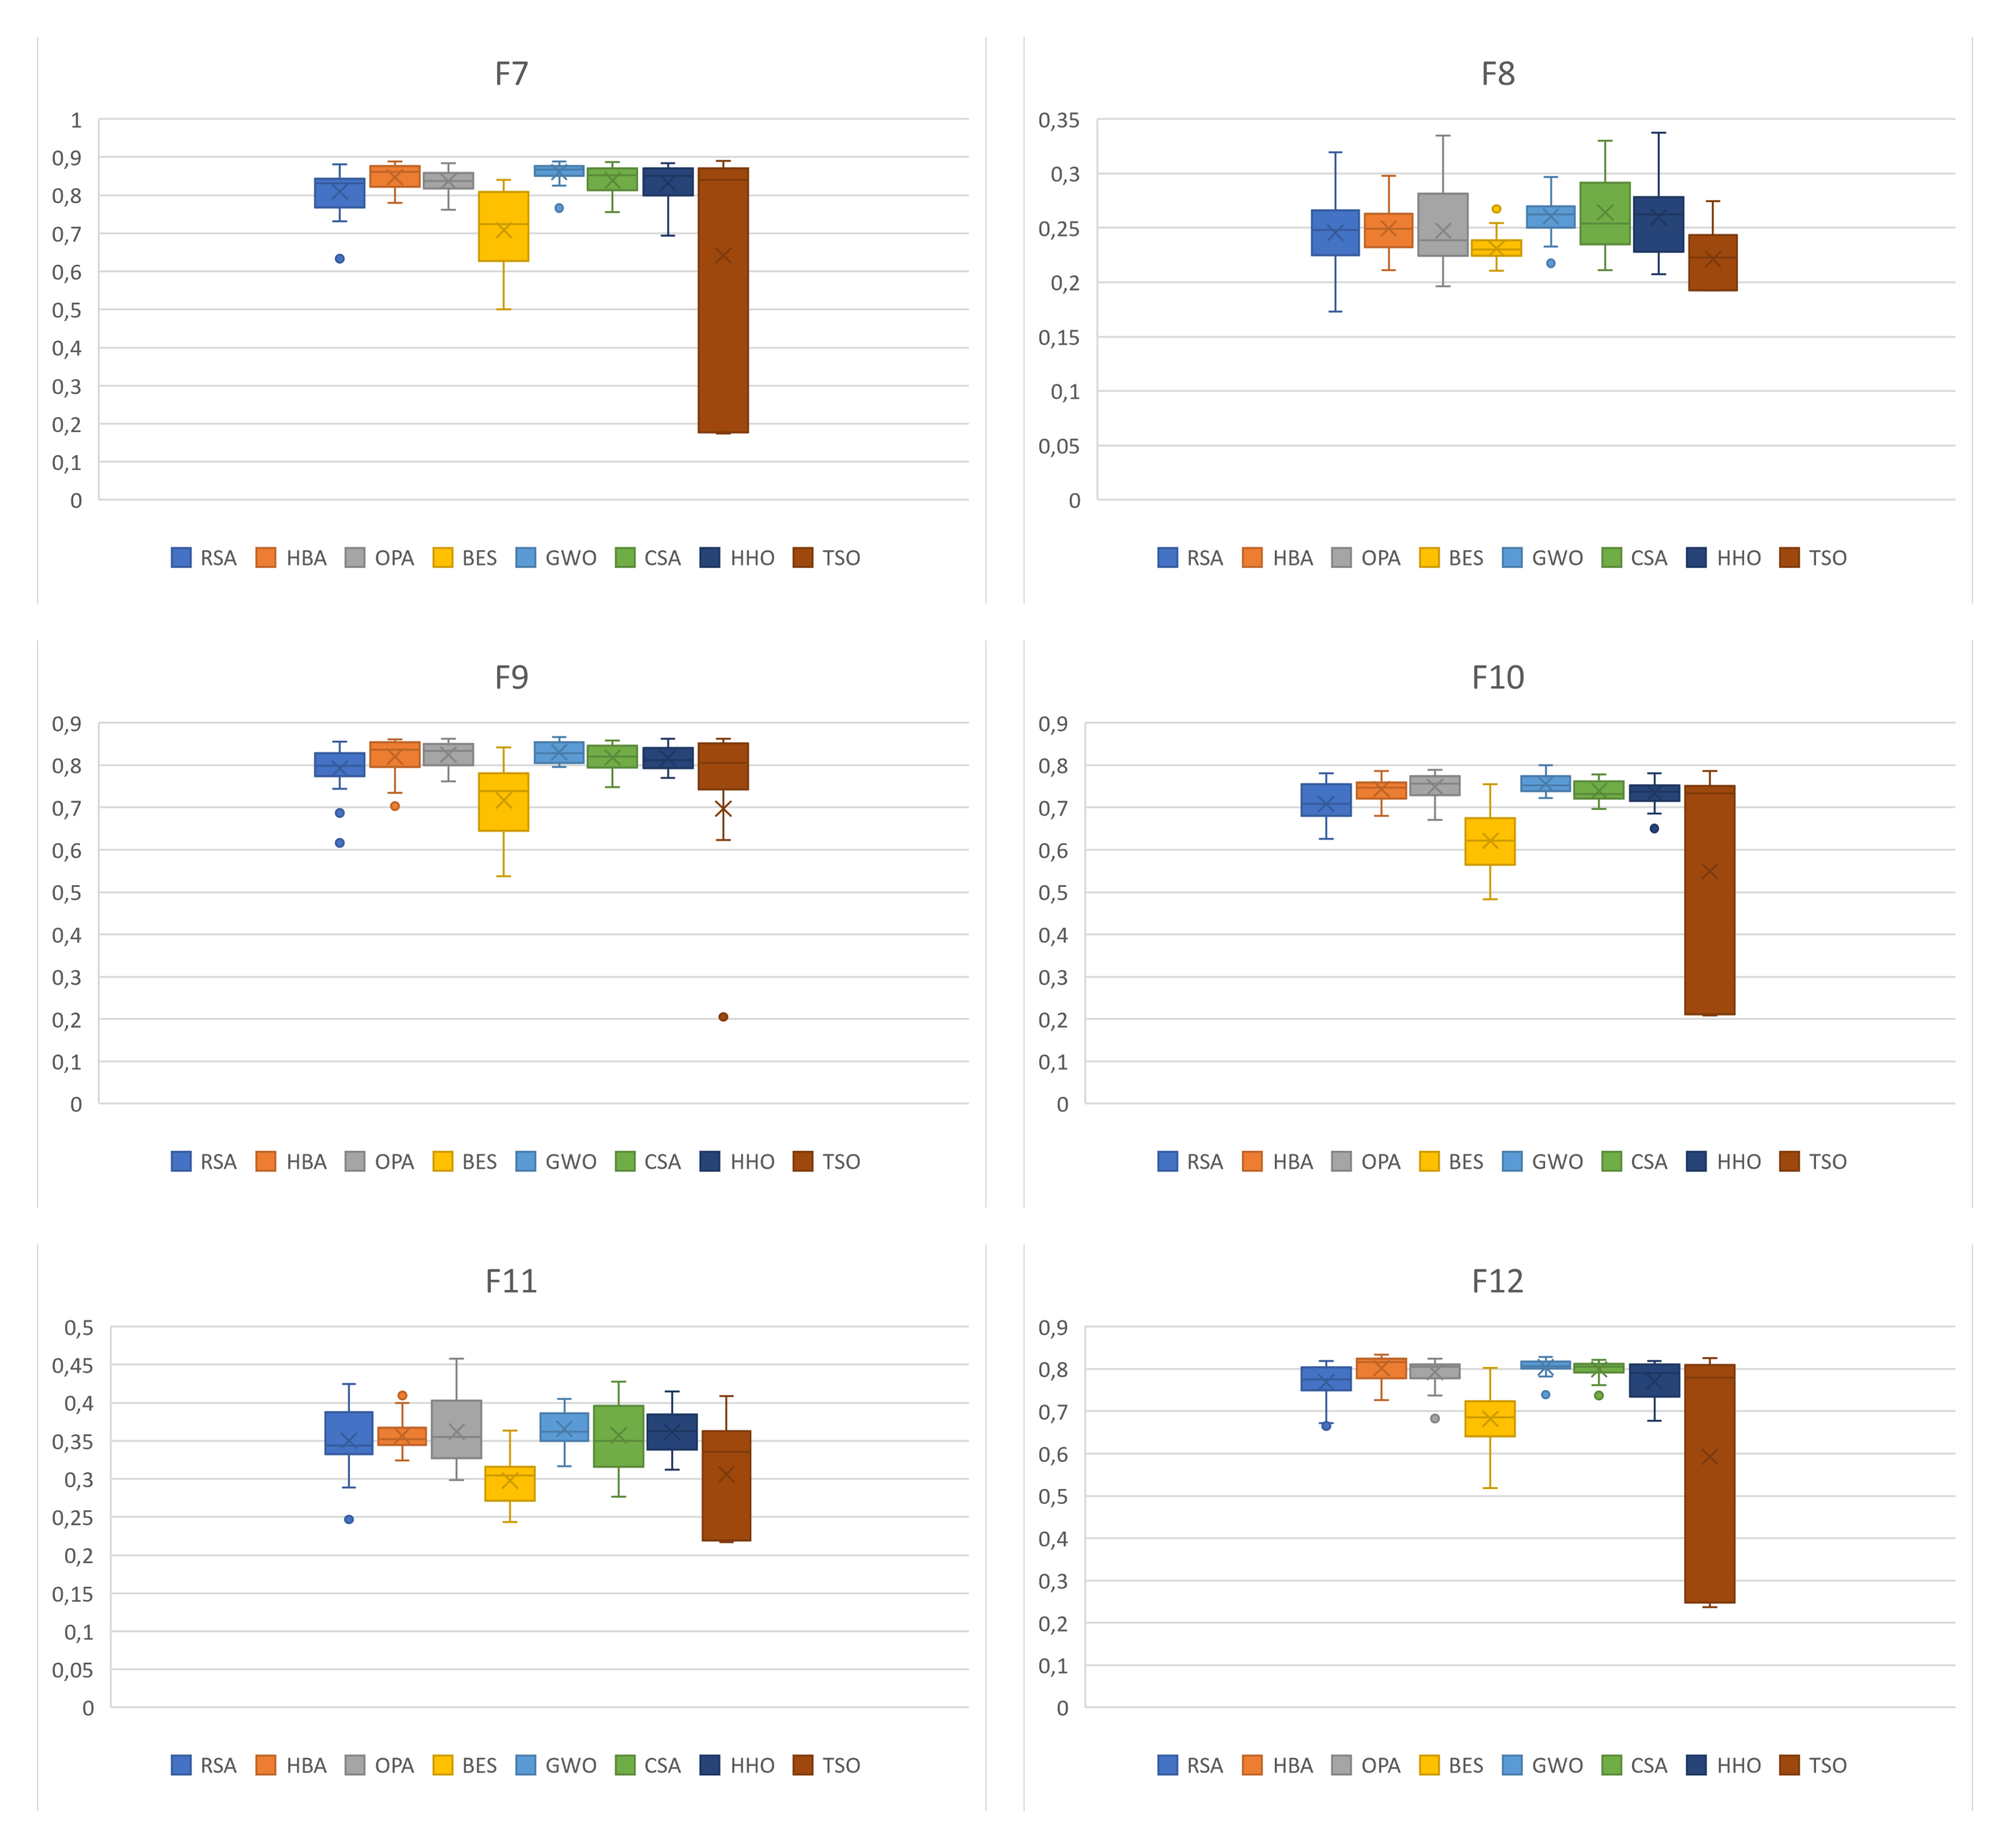
\includegraphics[width=\linewidth]{SSIM/Kapur/Dim9/SSIM_Dim9_Kapur_7_12.png}
	\end{subfigure}
	\begin{subfigure}{0.4\textwidth}
		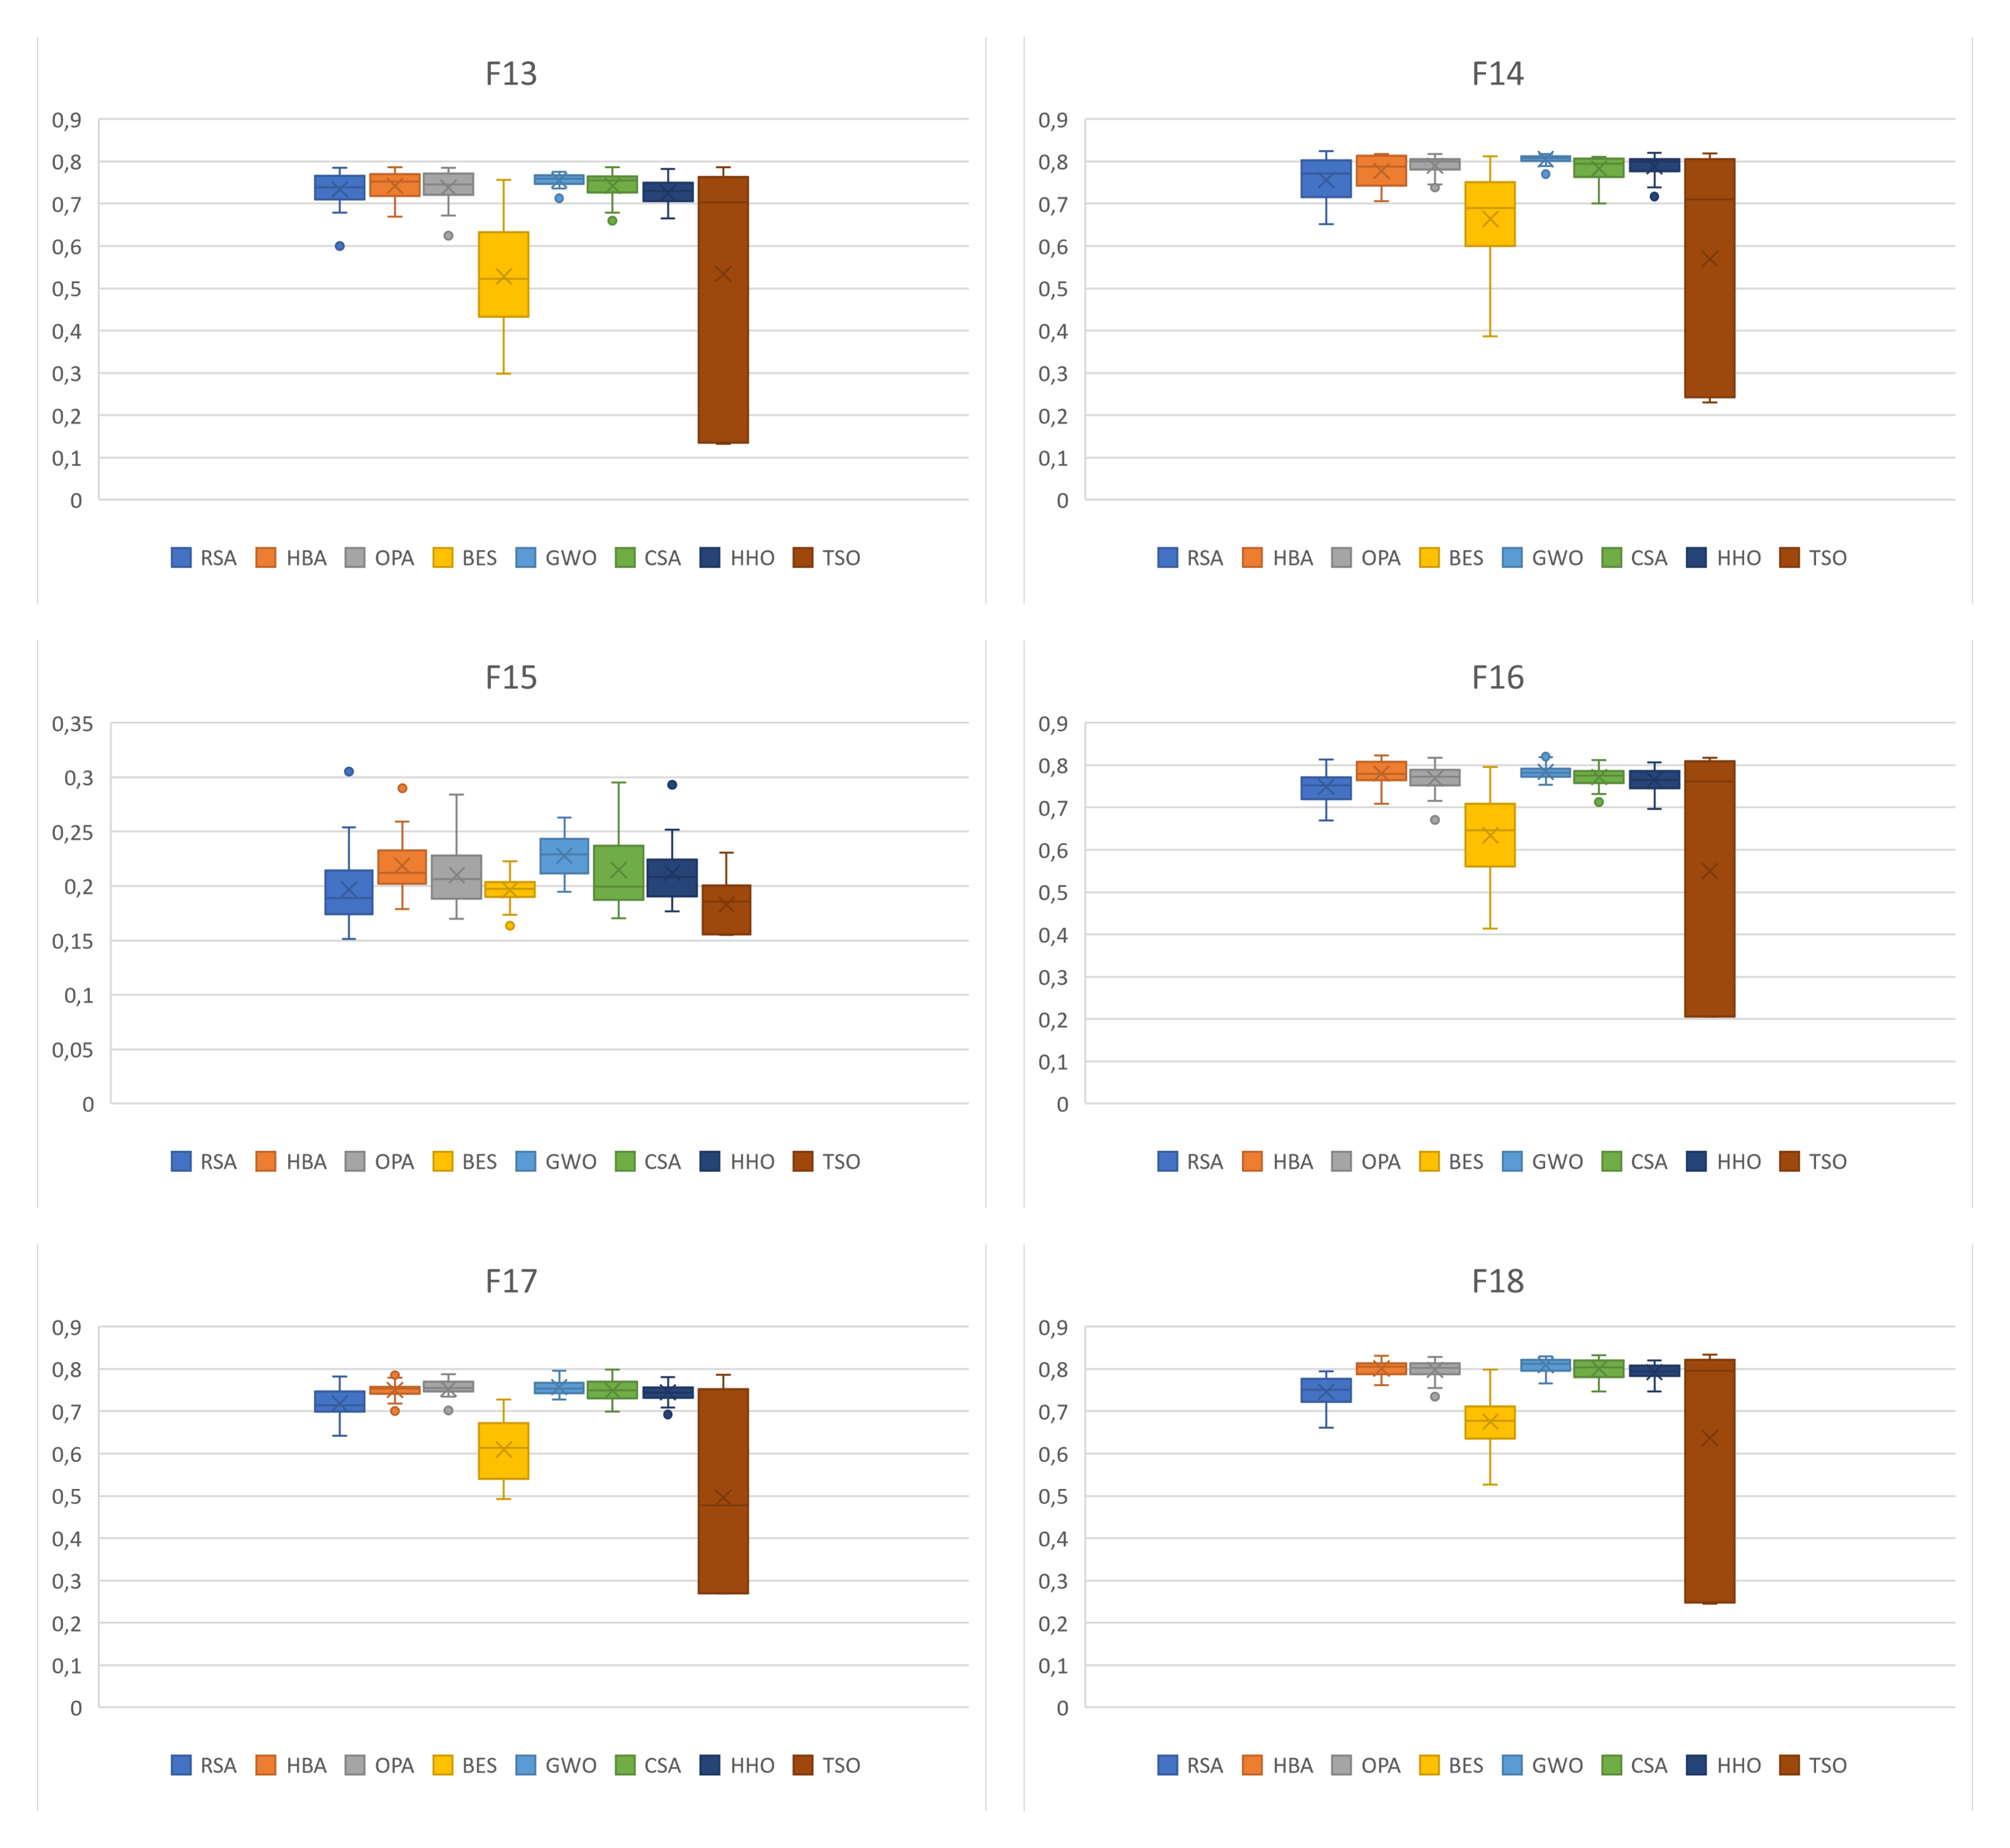
\includegraphics[width=\linewidth]{SSIM/Kapur/Dim9/SSIM_Dim9_Kapur_13_18.png}
		%\vspace{-150pt} % Ajusta este valor según sea necesario
	\end{subfigure}   
	\begin{subfigure}{0.4\textwidth}
		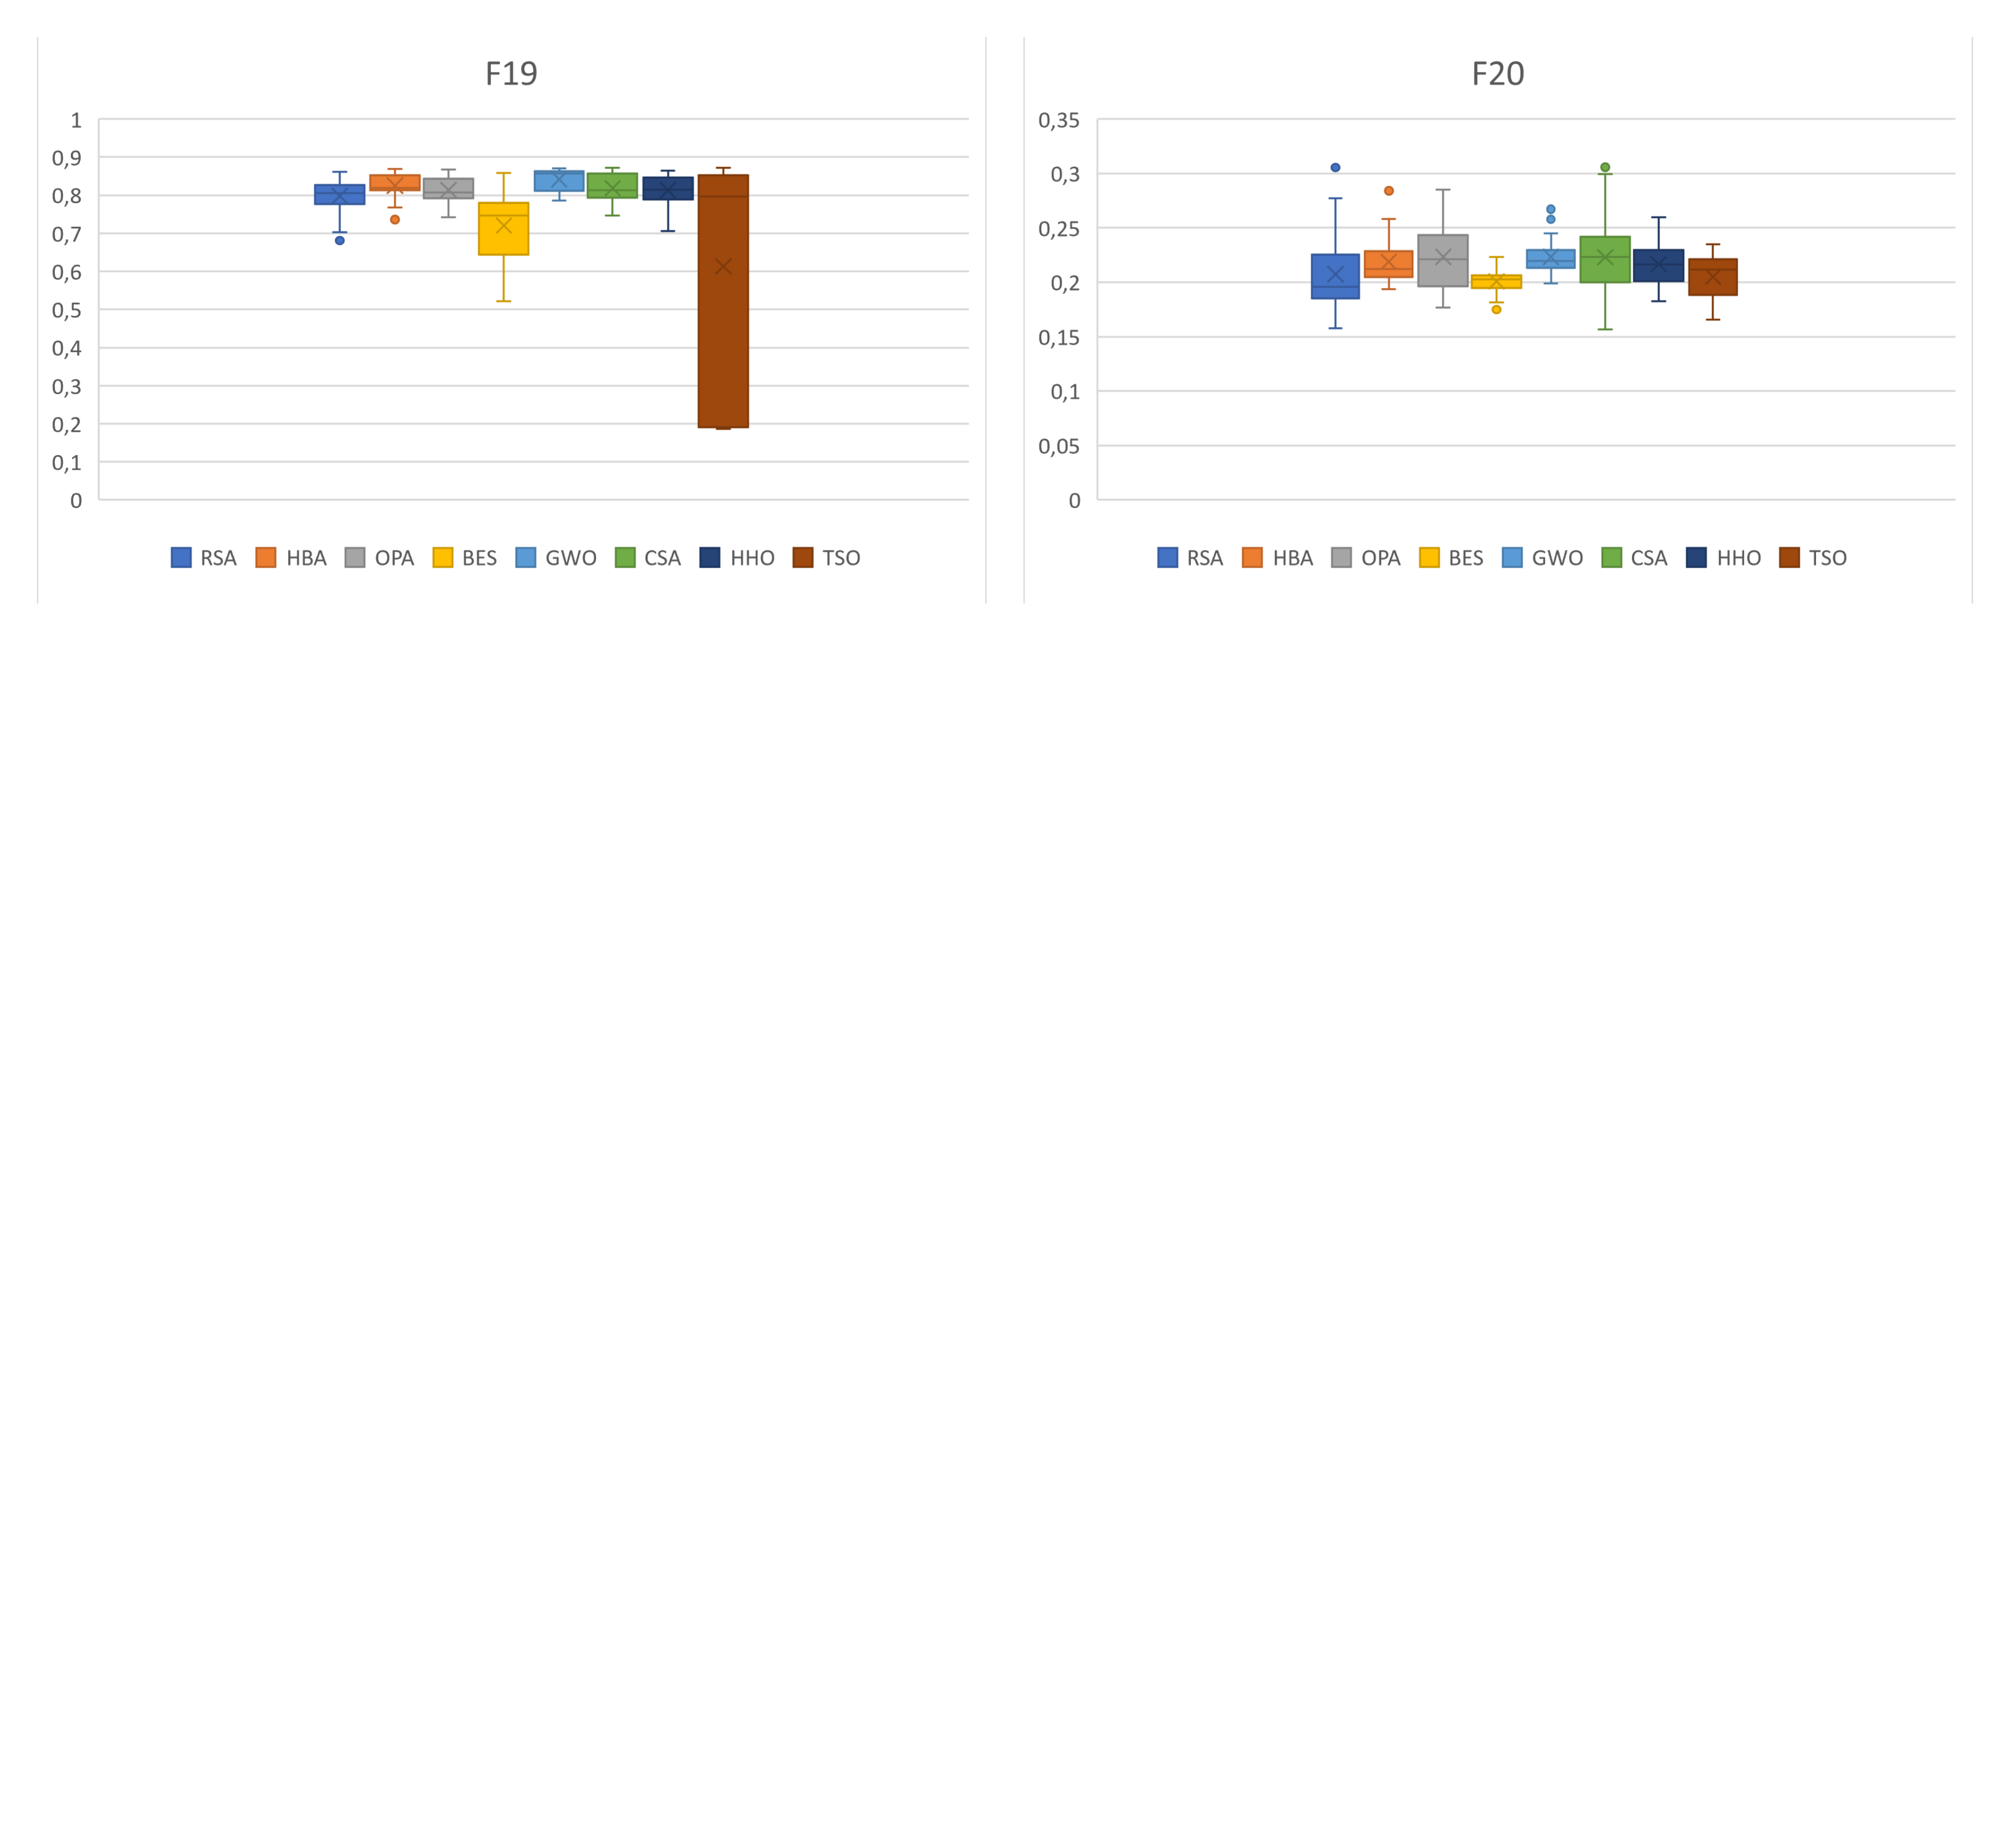
\includegraphics[width=\linewidth]{SSIM/Kapur/Dim9/SSIM_Dim9_Kapur_19_20.png}
		\vspace{-120pt} % Ajusta este valor según sea necesario
	\end{subfigure}
	\caption{Boxplot de los valores SSIM por cada imagen en la dimensión 9, desde la imagen 11 hasta la imagen 20,Función Entropía de Kapur}
	\label{fig:imagenes}    
\end{figure}
\subsection{Resultados Función Fitness Otsu}
\subsubsection{Dimensión 7}
\begin{itemize}
	\item RSA: Este algoritmo mostró un rendimiento inferior. Particularmente en F20, tenía la mediana más baja y valores atípicos significativos, indicando un rendimiento inconsistente y a menudo inferior a los demás.
	
	\item HBA: Presentó un rendimiento promedio a bueno, aunque con una variabilidad considerable en algunos casos. No fue el más destacado en ninguna función específica pero mantuvo una posición media en la mayoría de ellas.
	
	\item OPA: Registró resultados promedio con una consistencia aceptable. No tuvo los valores más altos, pero tampoco mostró una variabilidad extrema, lo que sugiere un rendimiento fiable.
	
	\item BES: Este algoritmo demostró un nivel de consistencia razonablemente bueno en las pruebas, manteniendo posiciones intermedias sin una gran cantidad de valores atípicos, lo que indica una robustez aceptable.
	
	\item CSA: Con resultados mixtos, este algoritmo mostró una consistencia regular y se mantuvo en un rango medio en la mayoría de las evaluaciones.
	
	\item HHO: Ofreció un buen rendimiento, especialmente en F19 y F20, con medianas altas y cajas estrechas que sugieren un alto nivel de consistencia y fiabilidad.
	
	\item GWO: Destacó consistentemente como uno de los algoritmos de mejor rendimiento en todas las funciones de fitness analizadas. En particular, fue el mejor en F8 y mantuvo un alto nivel de consistencia con resultados robustos en las demás funciones, lo que indica que es un algoritmo de optimización muy eficaz y confiable.
	
	\item TSO: Aunque tuvo un rendimiento variado, se destacó particularmente en F19 y F20, donde mostró las medianas más altas. A pesar de algunos valores atípicos, su rendimiento general fue uno de los mejores, lo que lo convierte en un algoritmo digno de consideración en problemas de optimización complejos.
	
\end{itemize}
\noindent En resumen, mientras que GWO y TSO se destacaron por su alto rendimiento, cada algoritmo tiene sus propias fortalezas y debilidades. GWO demostró ser el más consistente y eficaz en general, mientras que TSO mostró ser capaz de alcanzar los mejores valores de fitness en ciertas instancias, aunque con una variabilidad más notable
%Dimension 7
\begin{figure}
	\centering
	
	\begin{subfigure}{0.4\textwidth}
		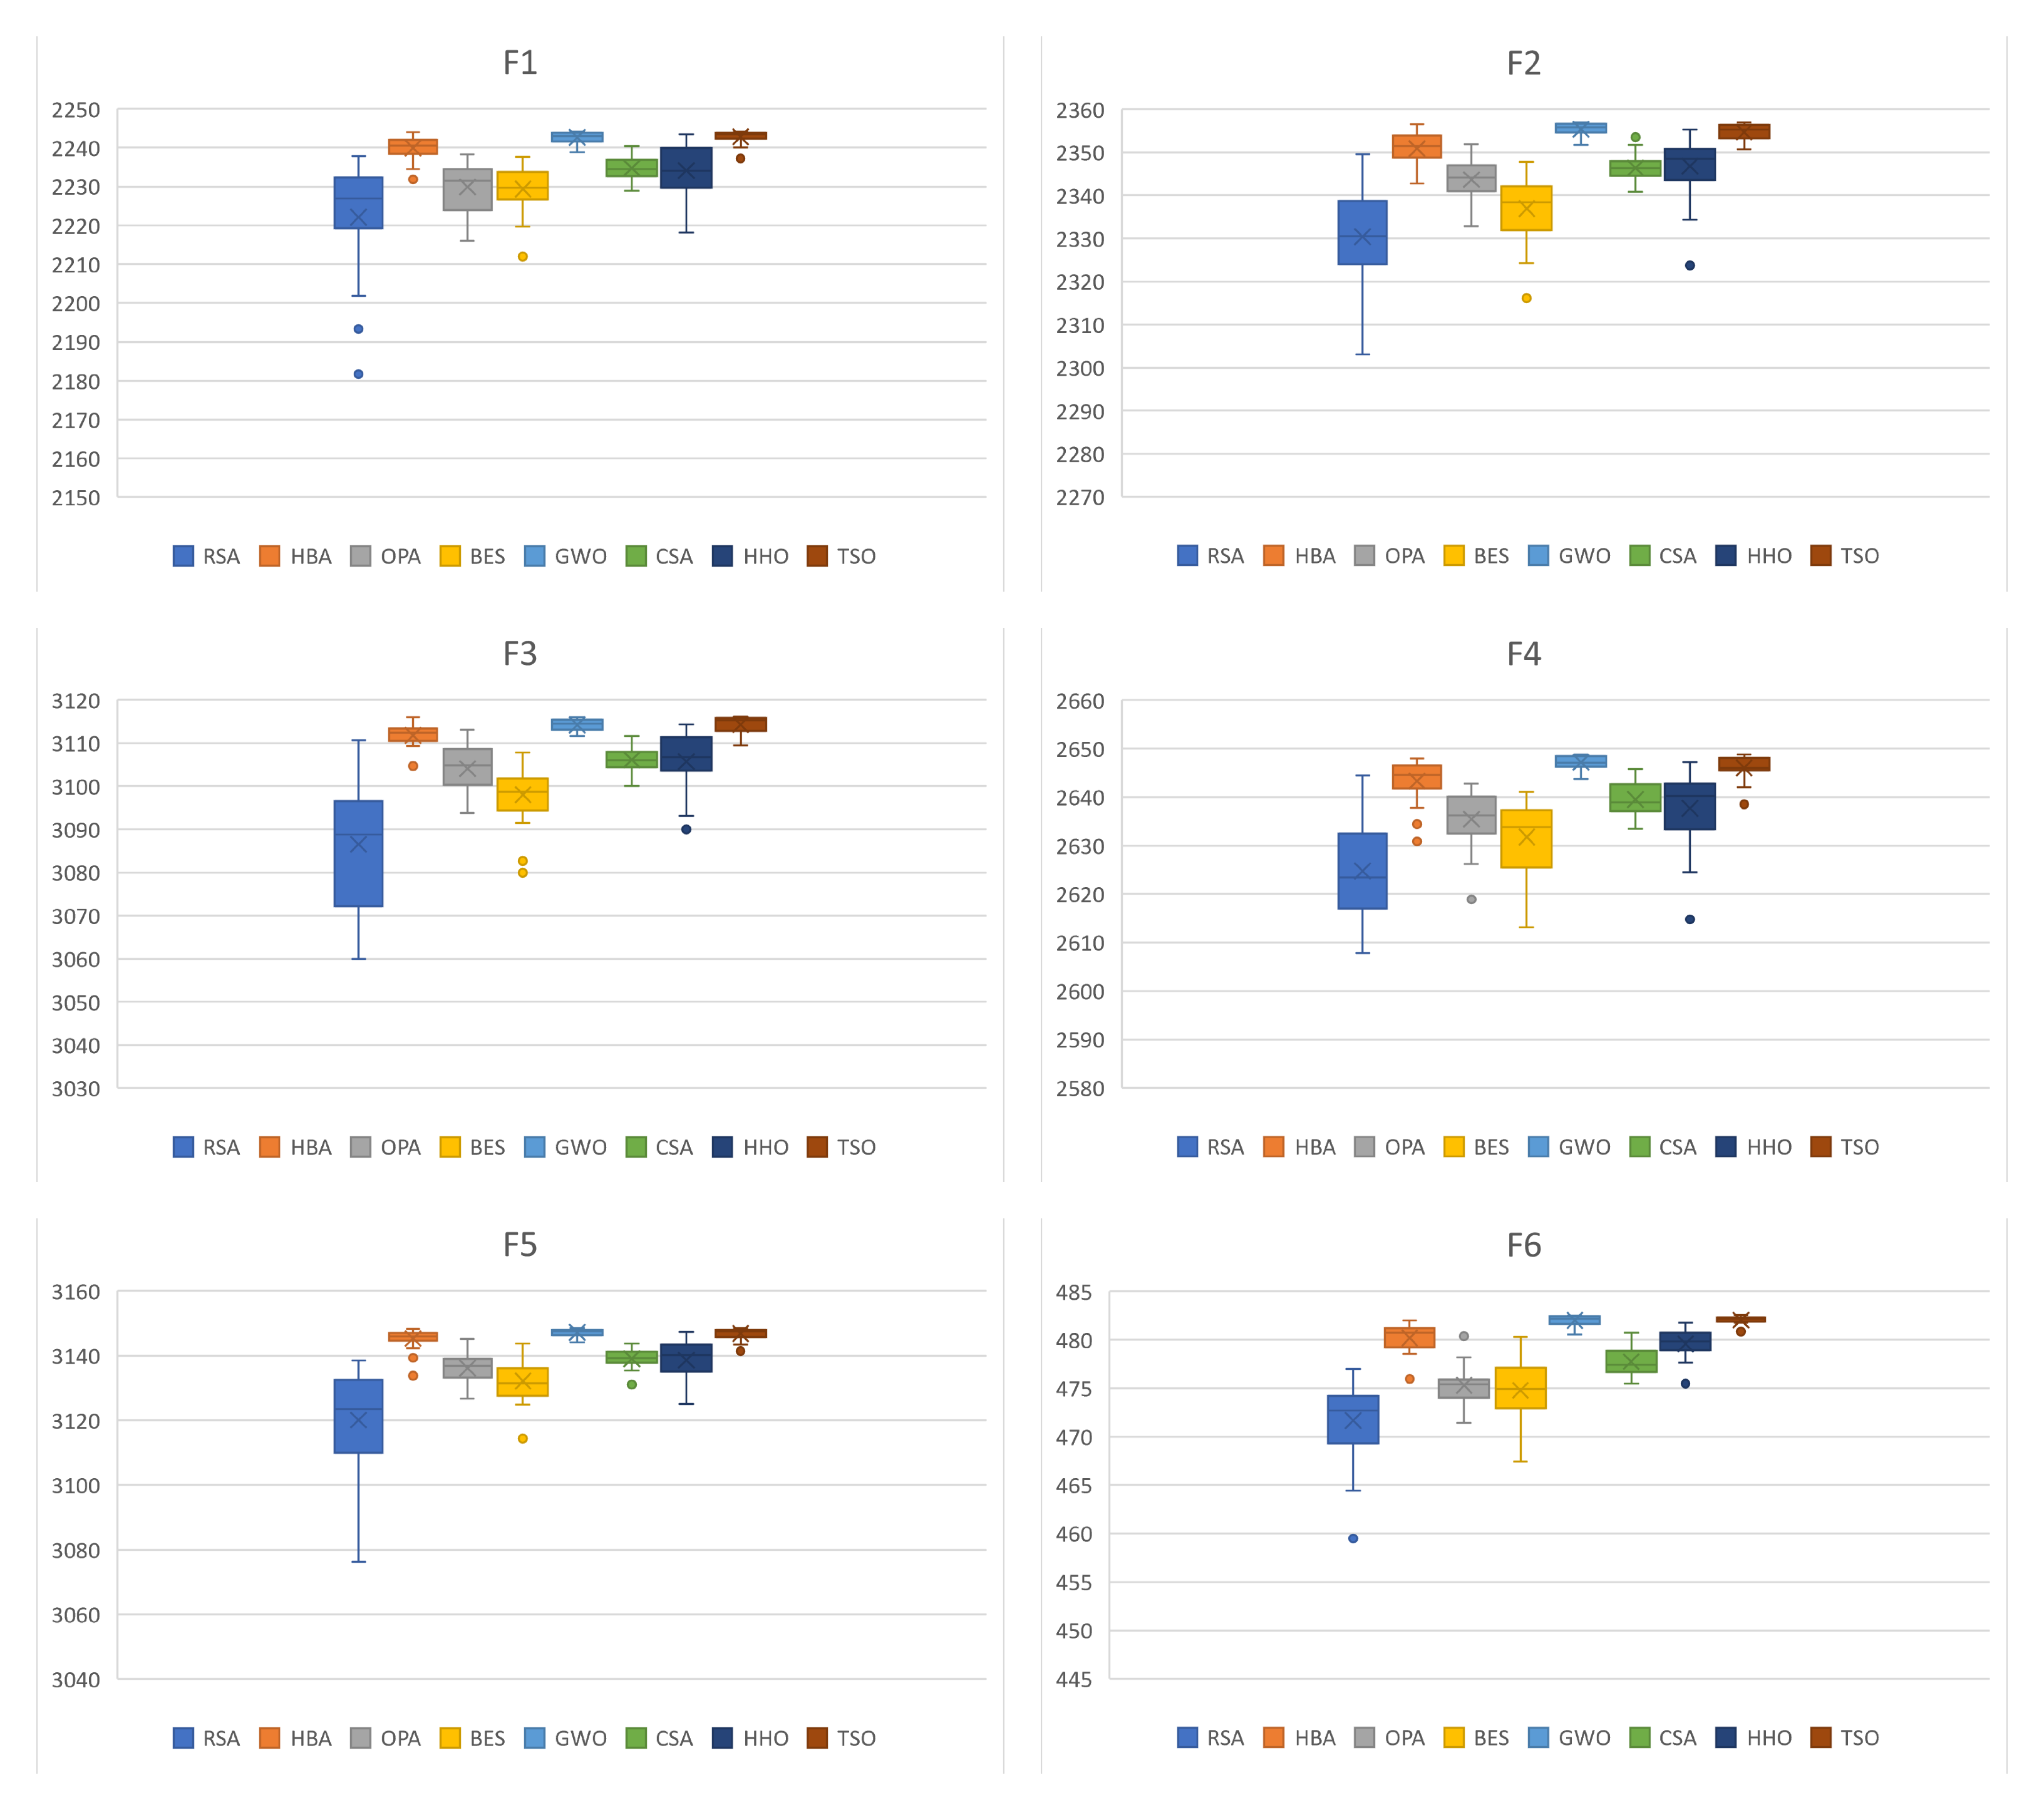
\includegraphics[width=\linewidth]{Fitness/Otsu/Boxplot_Dim7/BoxPlots_1-6_Dim7.png}
	\end{subfigure}
	
	\begin{subfigure}{0.4\textwidth}
		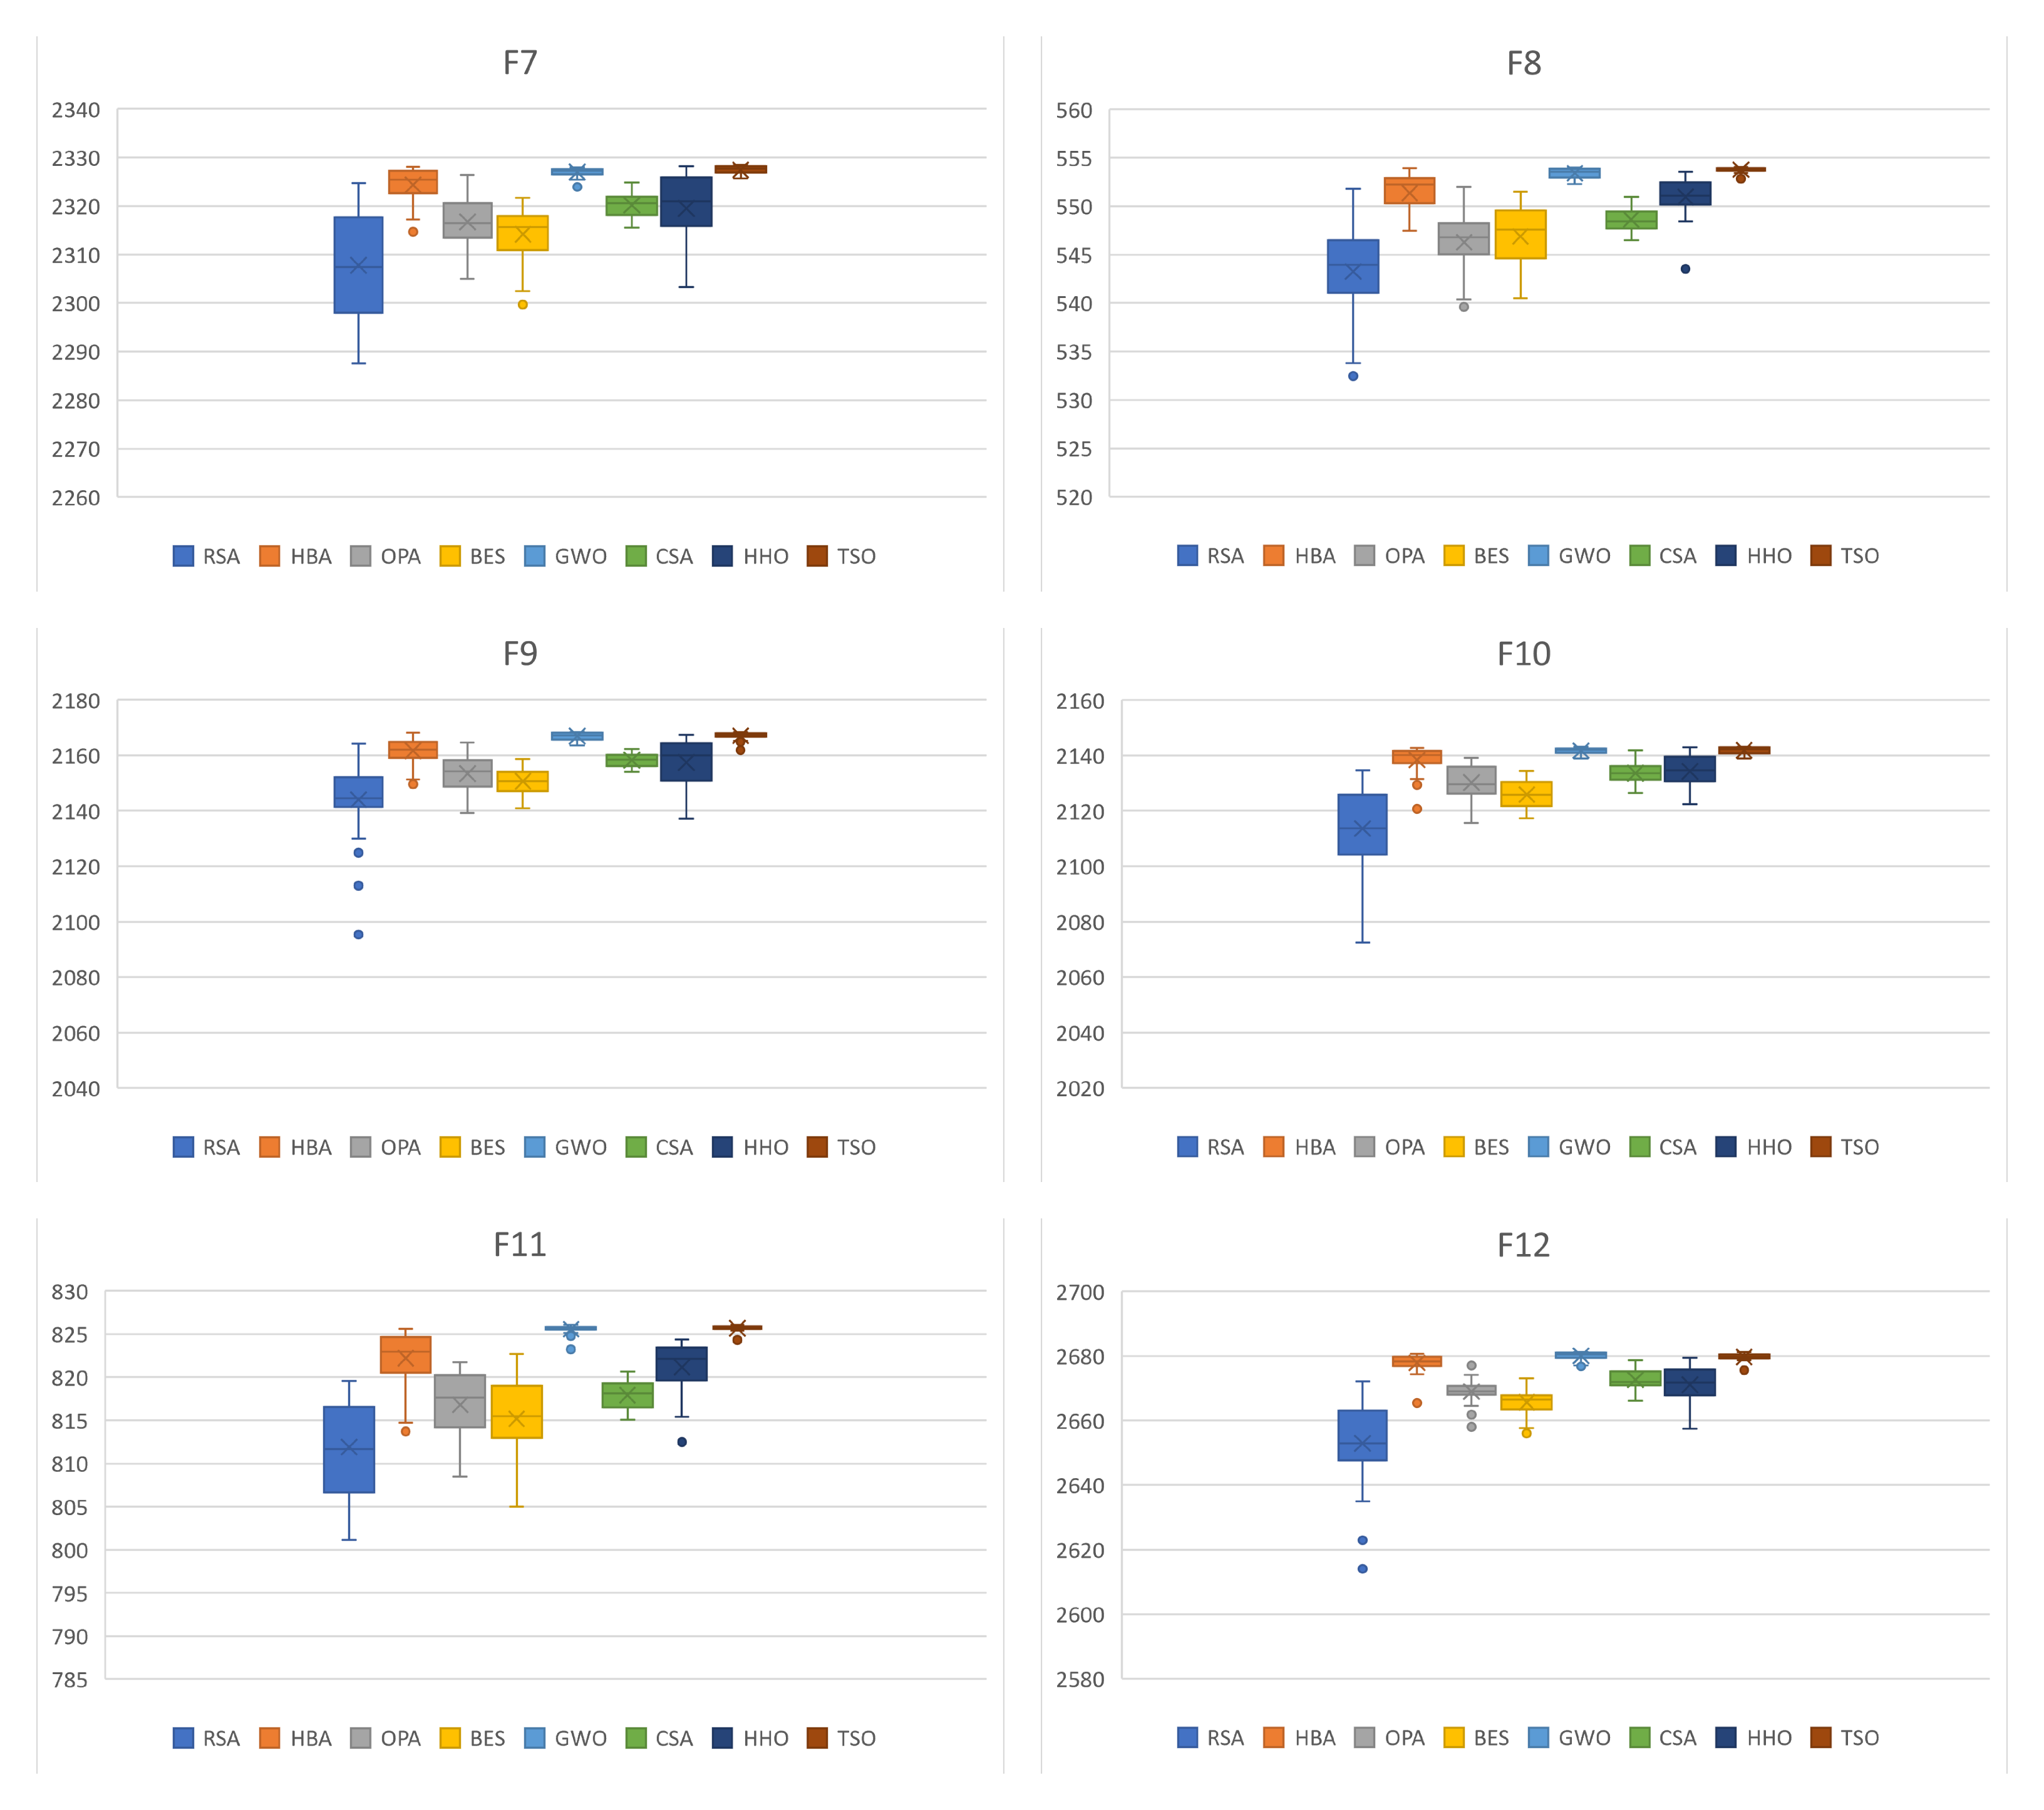
\includegraphics[width=\linewidth]{Fitness/Otsu/Boxplot_Dim7/BoxPlots_7-12_Dim7.png}
	\end{subfigure}
	\begin{subfigure}{0.4\textwidth}
		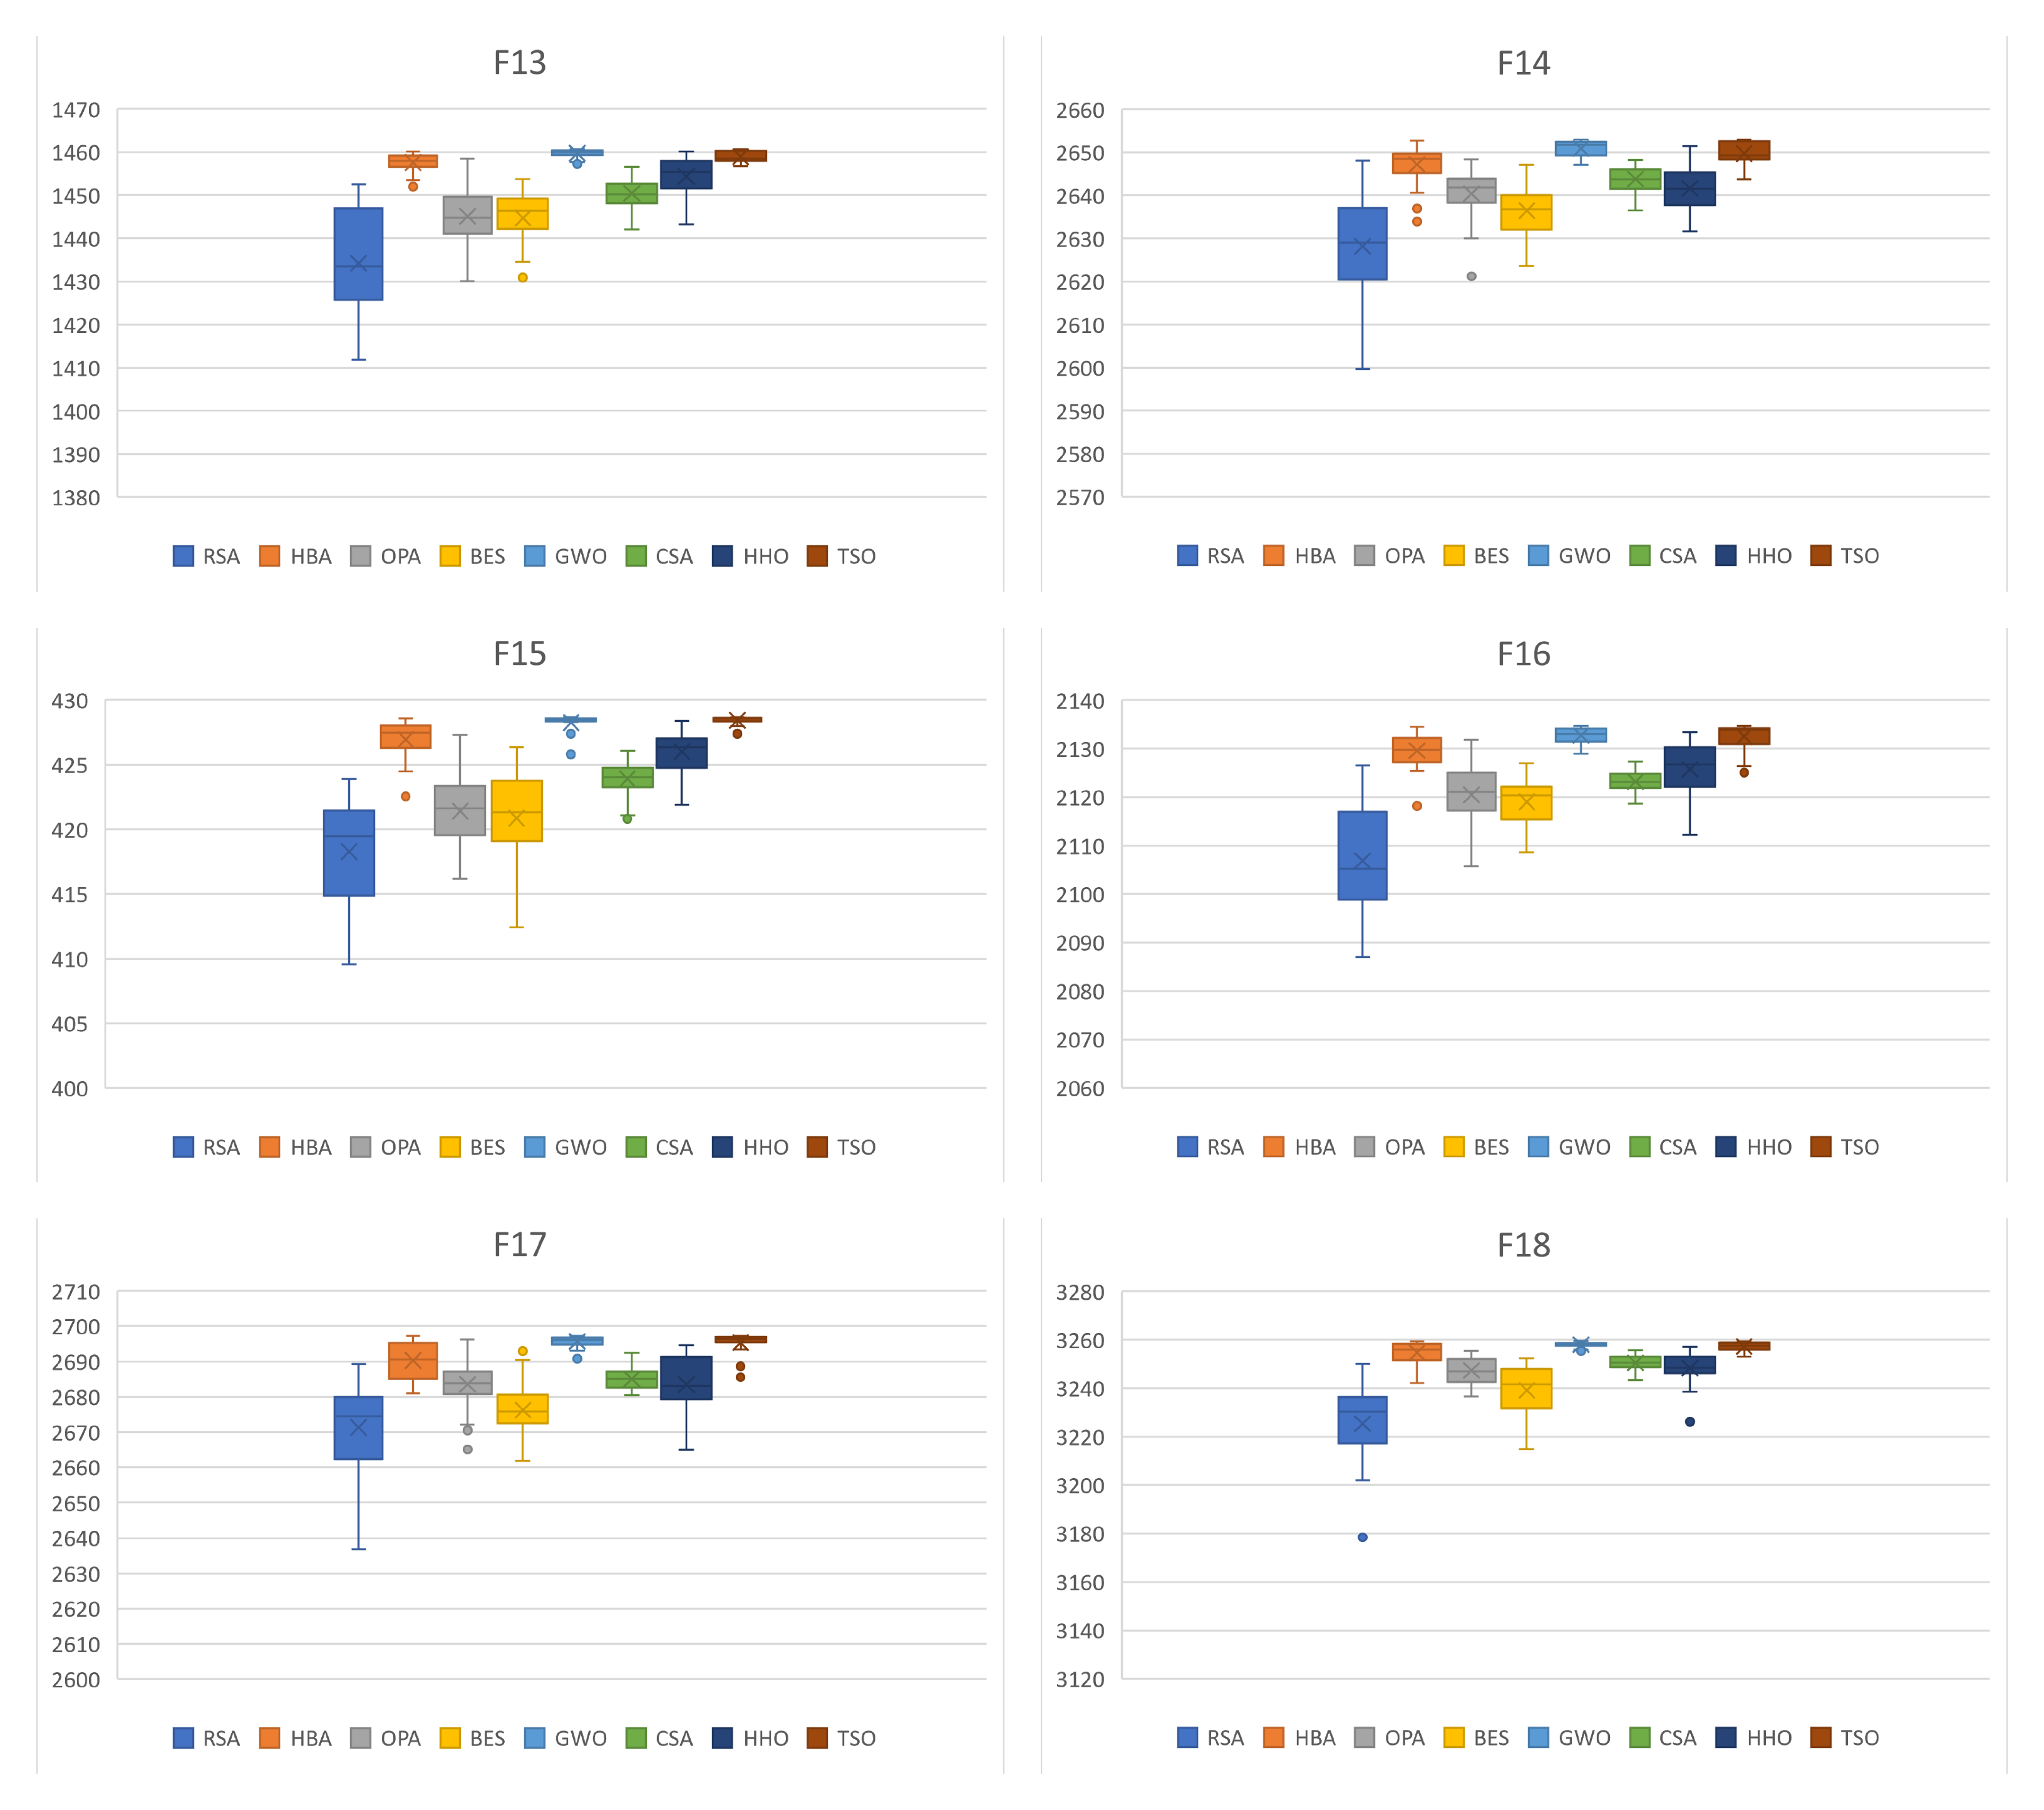
\includegraphics[width=\linewidth]{Fitness/Otsu/Boxplot_Dim7/BoxPlots_13-18_Dim7.png}
	\end{subfigure}
	\begin{subfigure}{0.4\textwidth}
		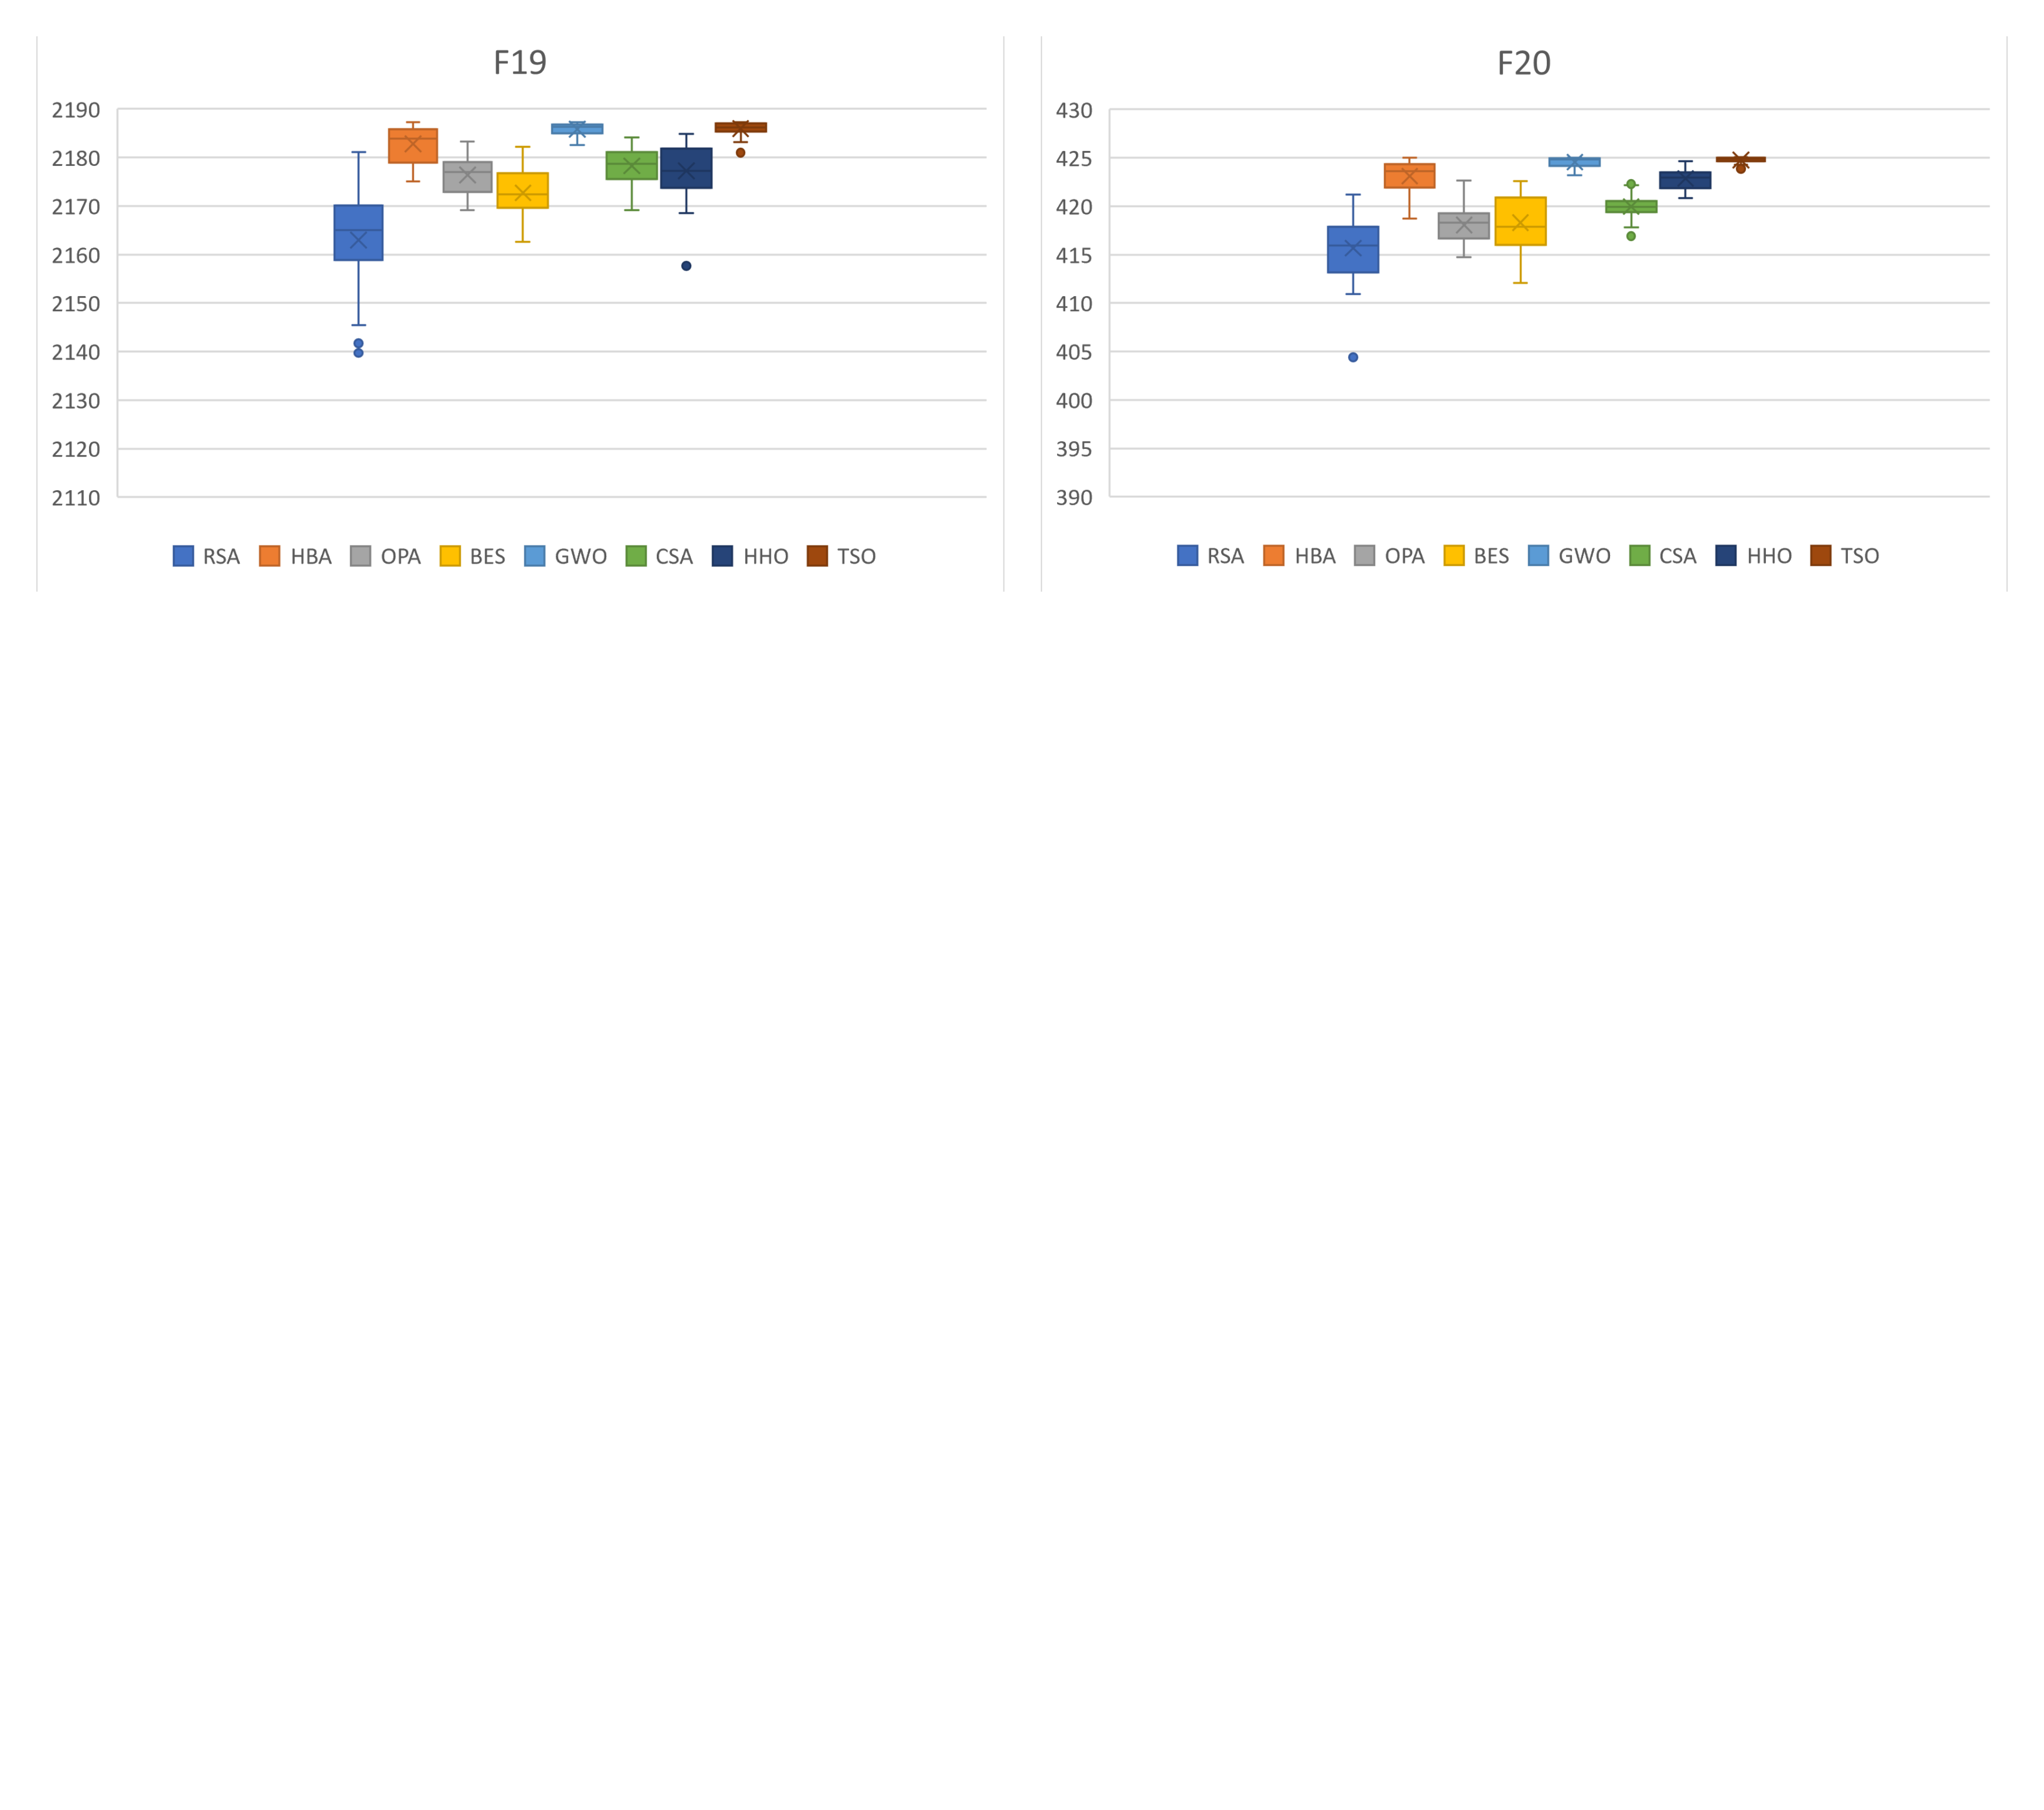
\includegraphics[width=\linewidth]{Fitness/Otsu/Boxplot_Dim7/BoxPlots_19-20_Dim7.png}
		\vspace{-120pt} % Ajusta este valor según sea necesario
	\end{subfigure}
	\caption{Boxplot de los valores Fitness por cada imagen en la dimensión 7, desde la imagen 1 hasta la imagen 20,Función Objetivo Otsu}
	\label{fig:imagenes}    
\end{figure}
\subsubsection{Dimensión 8}
\begin{itemize}
	\item RSA: Su rendimiento varía considerablemente. Aunque en algunos casos se acerca a un rendimiento medio bueno, también ha mostrado ser susceptible a resultados muy variables. No se destaca como el mejor ni el peor consistentemente.
	
	\item HBA: Este algoritmo ha mostrado un rendimiento promedio. Aunque no es consistentemente el mejor o el peor, su rendimiento tiende a estar en un rango medio sin extremos marcados.
	
	\item OPA: Generalmente, OPA ha mostrado un rendimiento medio con una variabilidad moderada. No ha presentado los mejores resultados, pero tampoco los peores, ubicándose frecuentemente en un rango intermedio.
	
	\item BES: Tiene un rendimiento variable pero tiende a situarse en un rango medio. No ha demostrado ser el mejor ni el peor, aunque ocasionalmente presenta resultados subóptimos.
	
	\item GWO: Este algoritmo se ha destacado en varios de los boxplots como uno de los que tiene el mejor rendimiento, con medianas bajas y dispersión reducida, lo que indica resultados buenos y consistentes.
	
	\item CSA: CSA también ha mostrado un rendimiento bueno y consistente, con medianas bajas y poca dispersión, aunque no siempre tan destacado como GWO.
	
	\item HHO: Generalmente tiene un buen rendimiento, aunque en algunas mostró una mediana ligeramente más alta comparada con los mejores. Se puede considerar que tiene un rendimiento intermedio a bueno.
	
	\item TSO: En la mayoría de los boxplots, TSO ha mostrado tener el peor rendimiento, con medianas altas y una dispersión que indica resultados menos óptimos y mayor variabilidad.
	
\end{itemize}
\noindent Mejor Rendimiento: GWO se destaca consistentemente como el algoritmo con el mejor rendimiento.
Rendimiento Intermedio: HHO muestra un rendimiento generalmente bueno, pero no alcanza la consistencia del mejor algoritmo, ubicándose en un nivel intermedio.
% Dimension 8
\begin{figure}
	\centering
	
	\begin{subfigure}{0.4\textwidth}
		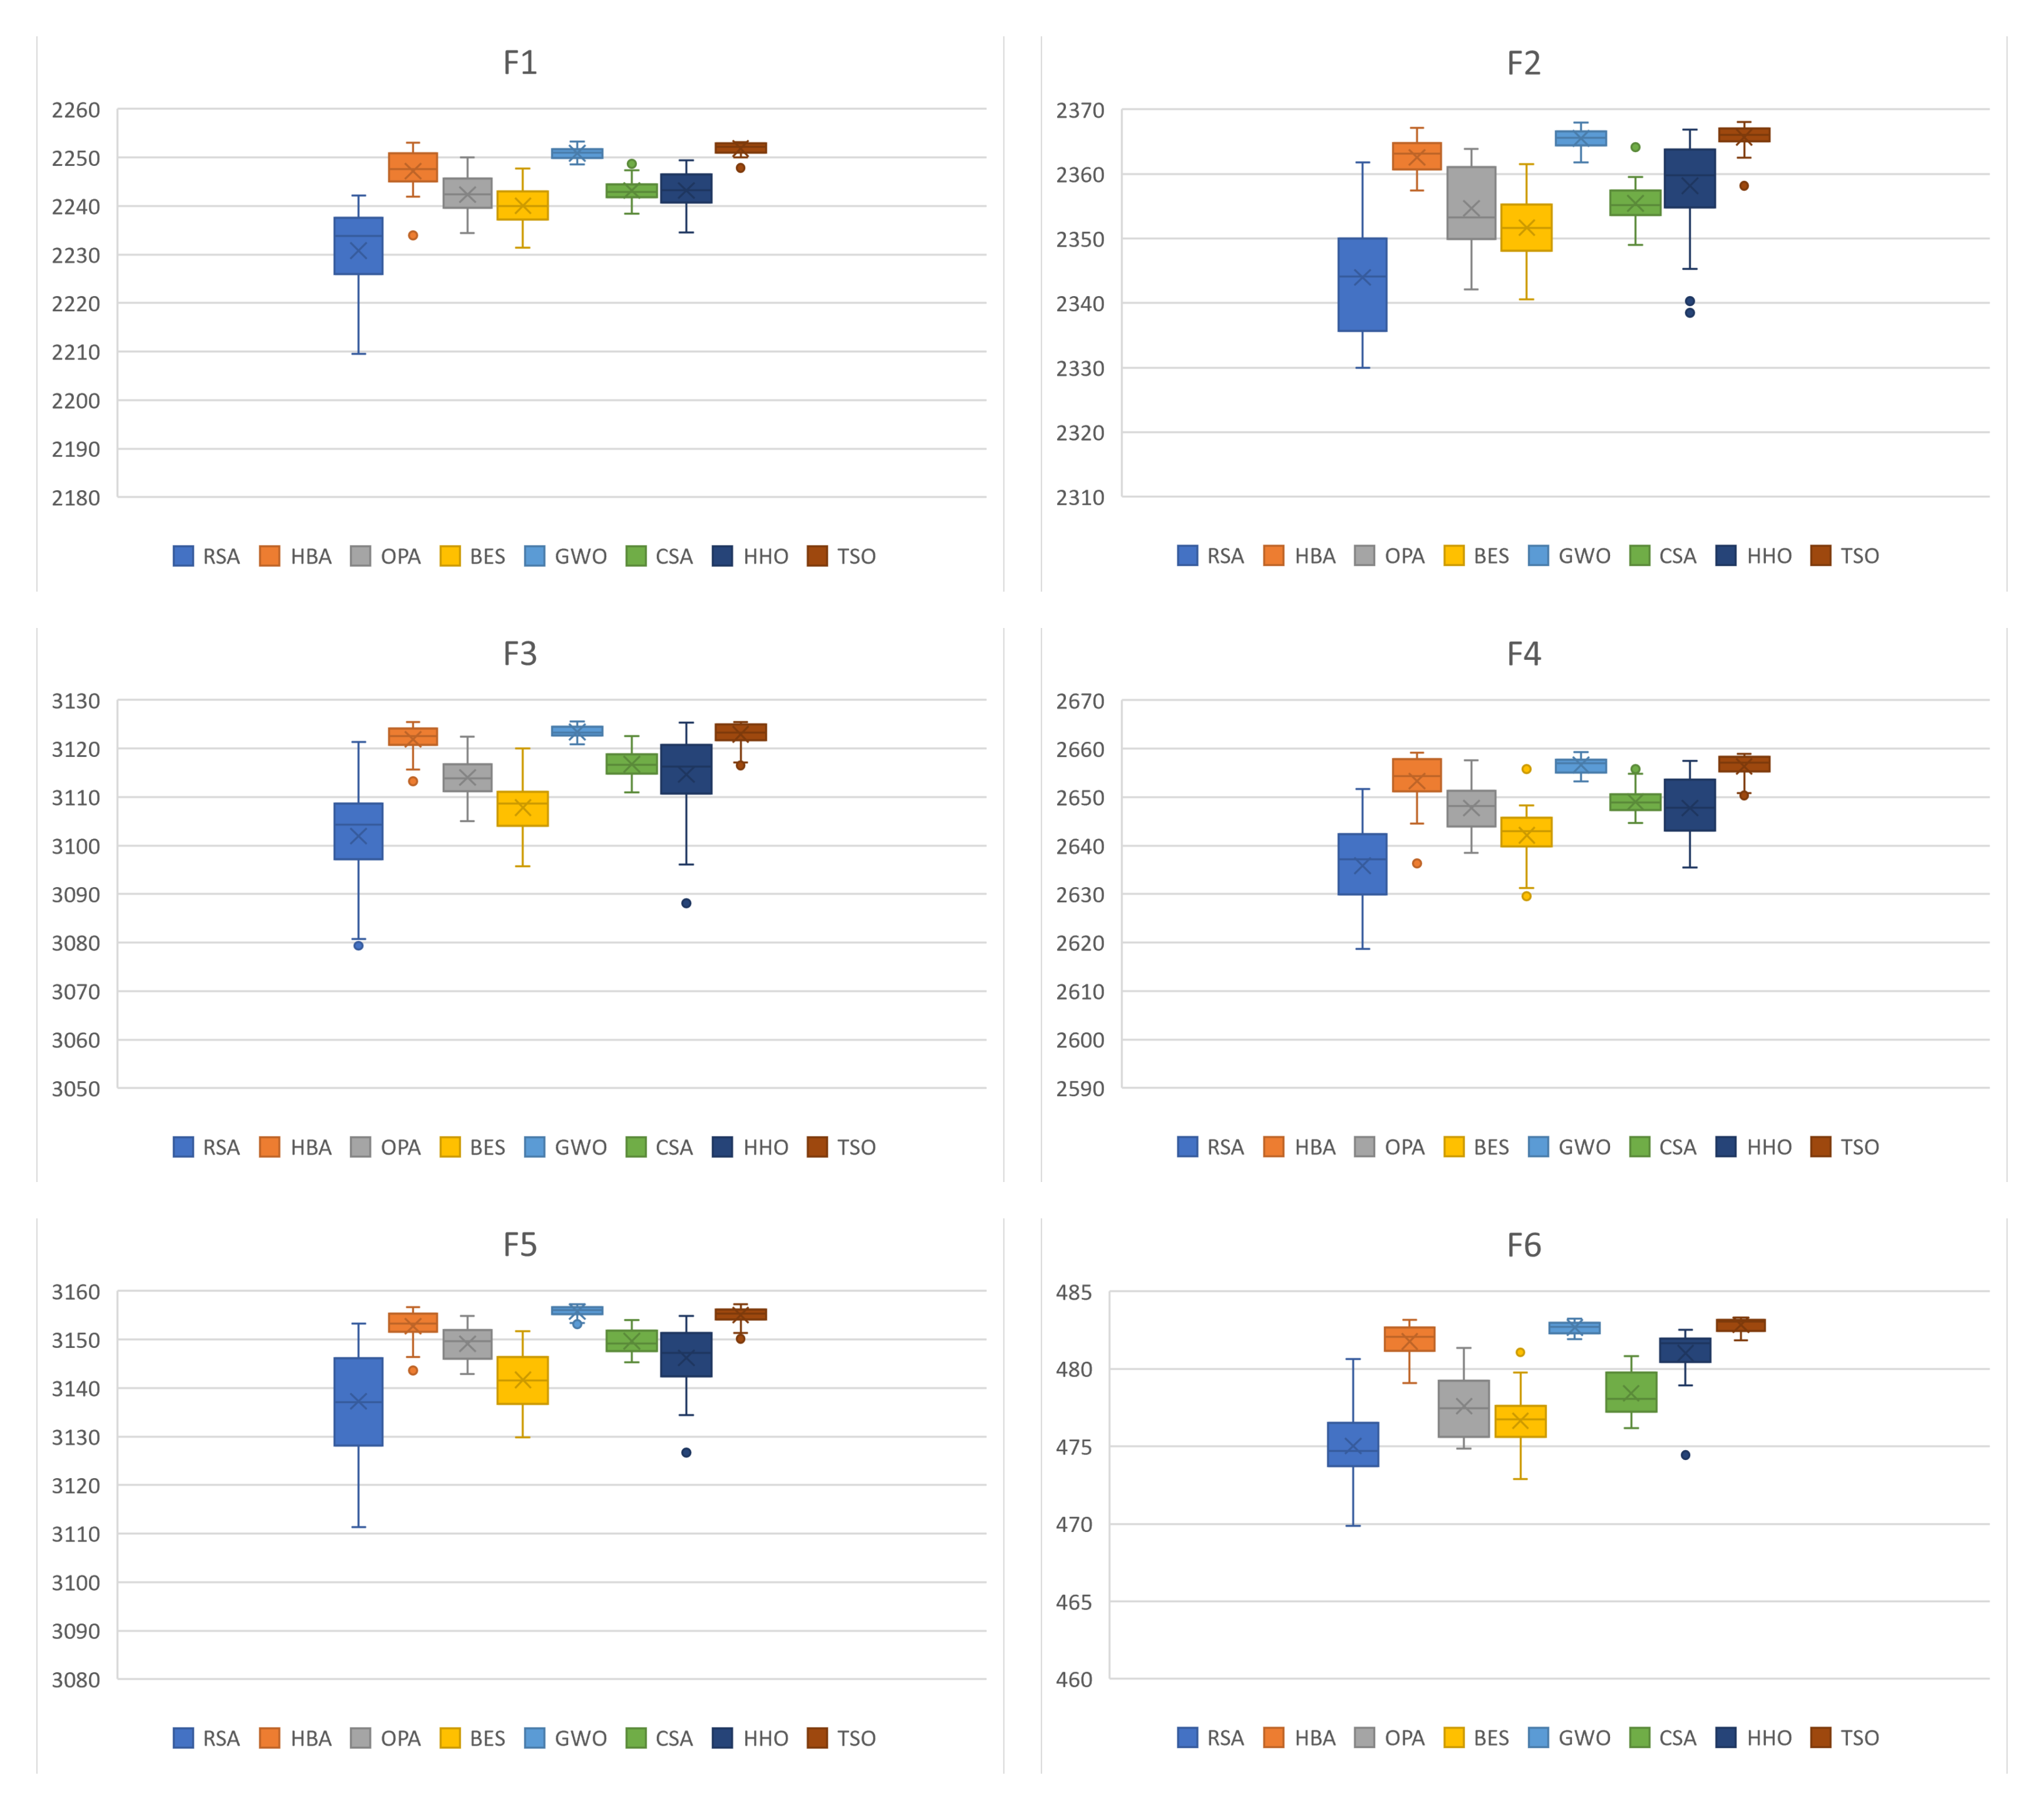
\includegraphics[width=\linewidth]{Fitness/Otsu/Boxplot_Dim8/BoxPlots_1-6_Dim8.png}
	\end{subfigure}
	
	\begin{subfigure}{0.4\textwidth}
		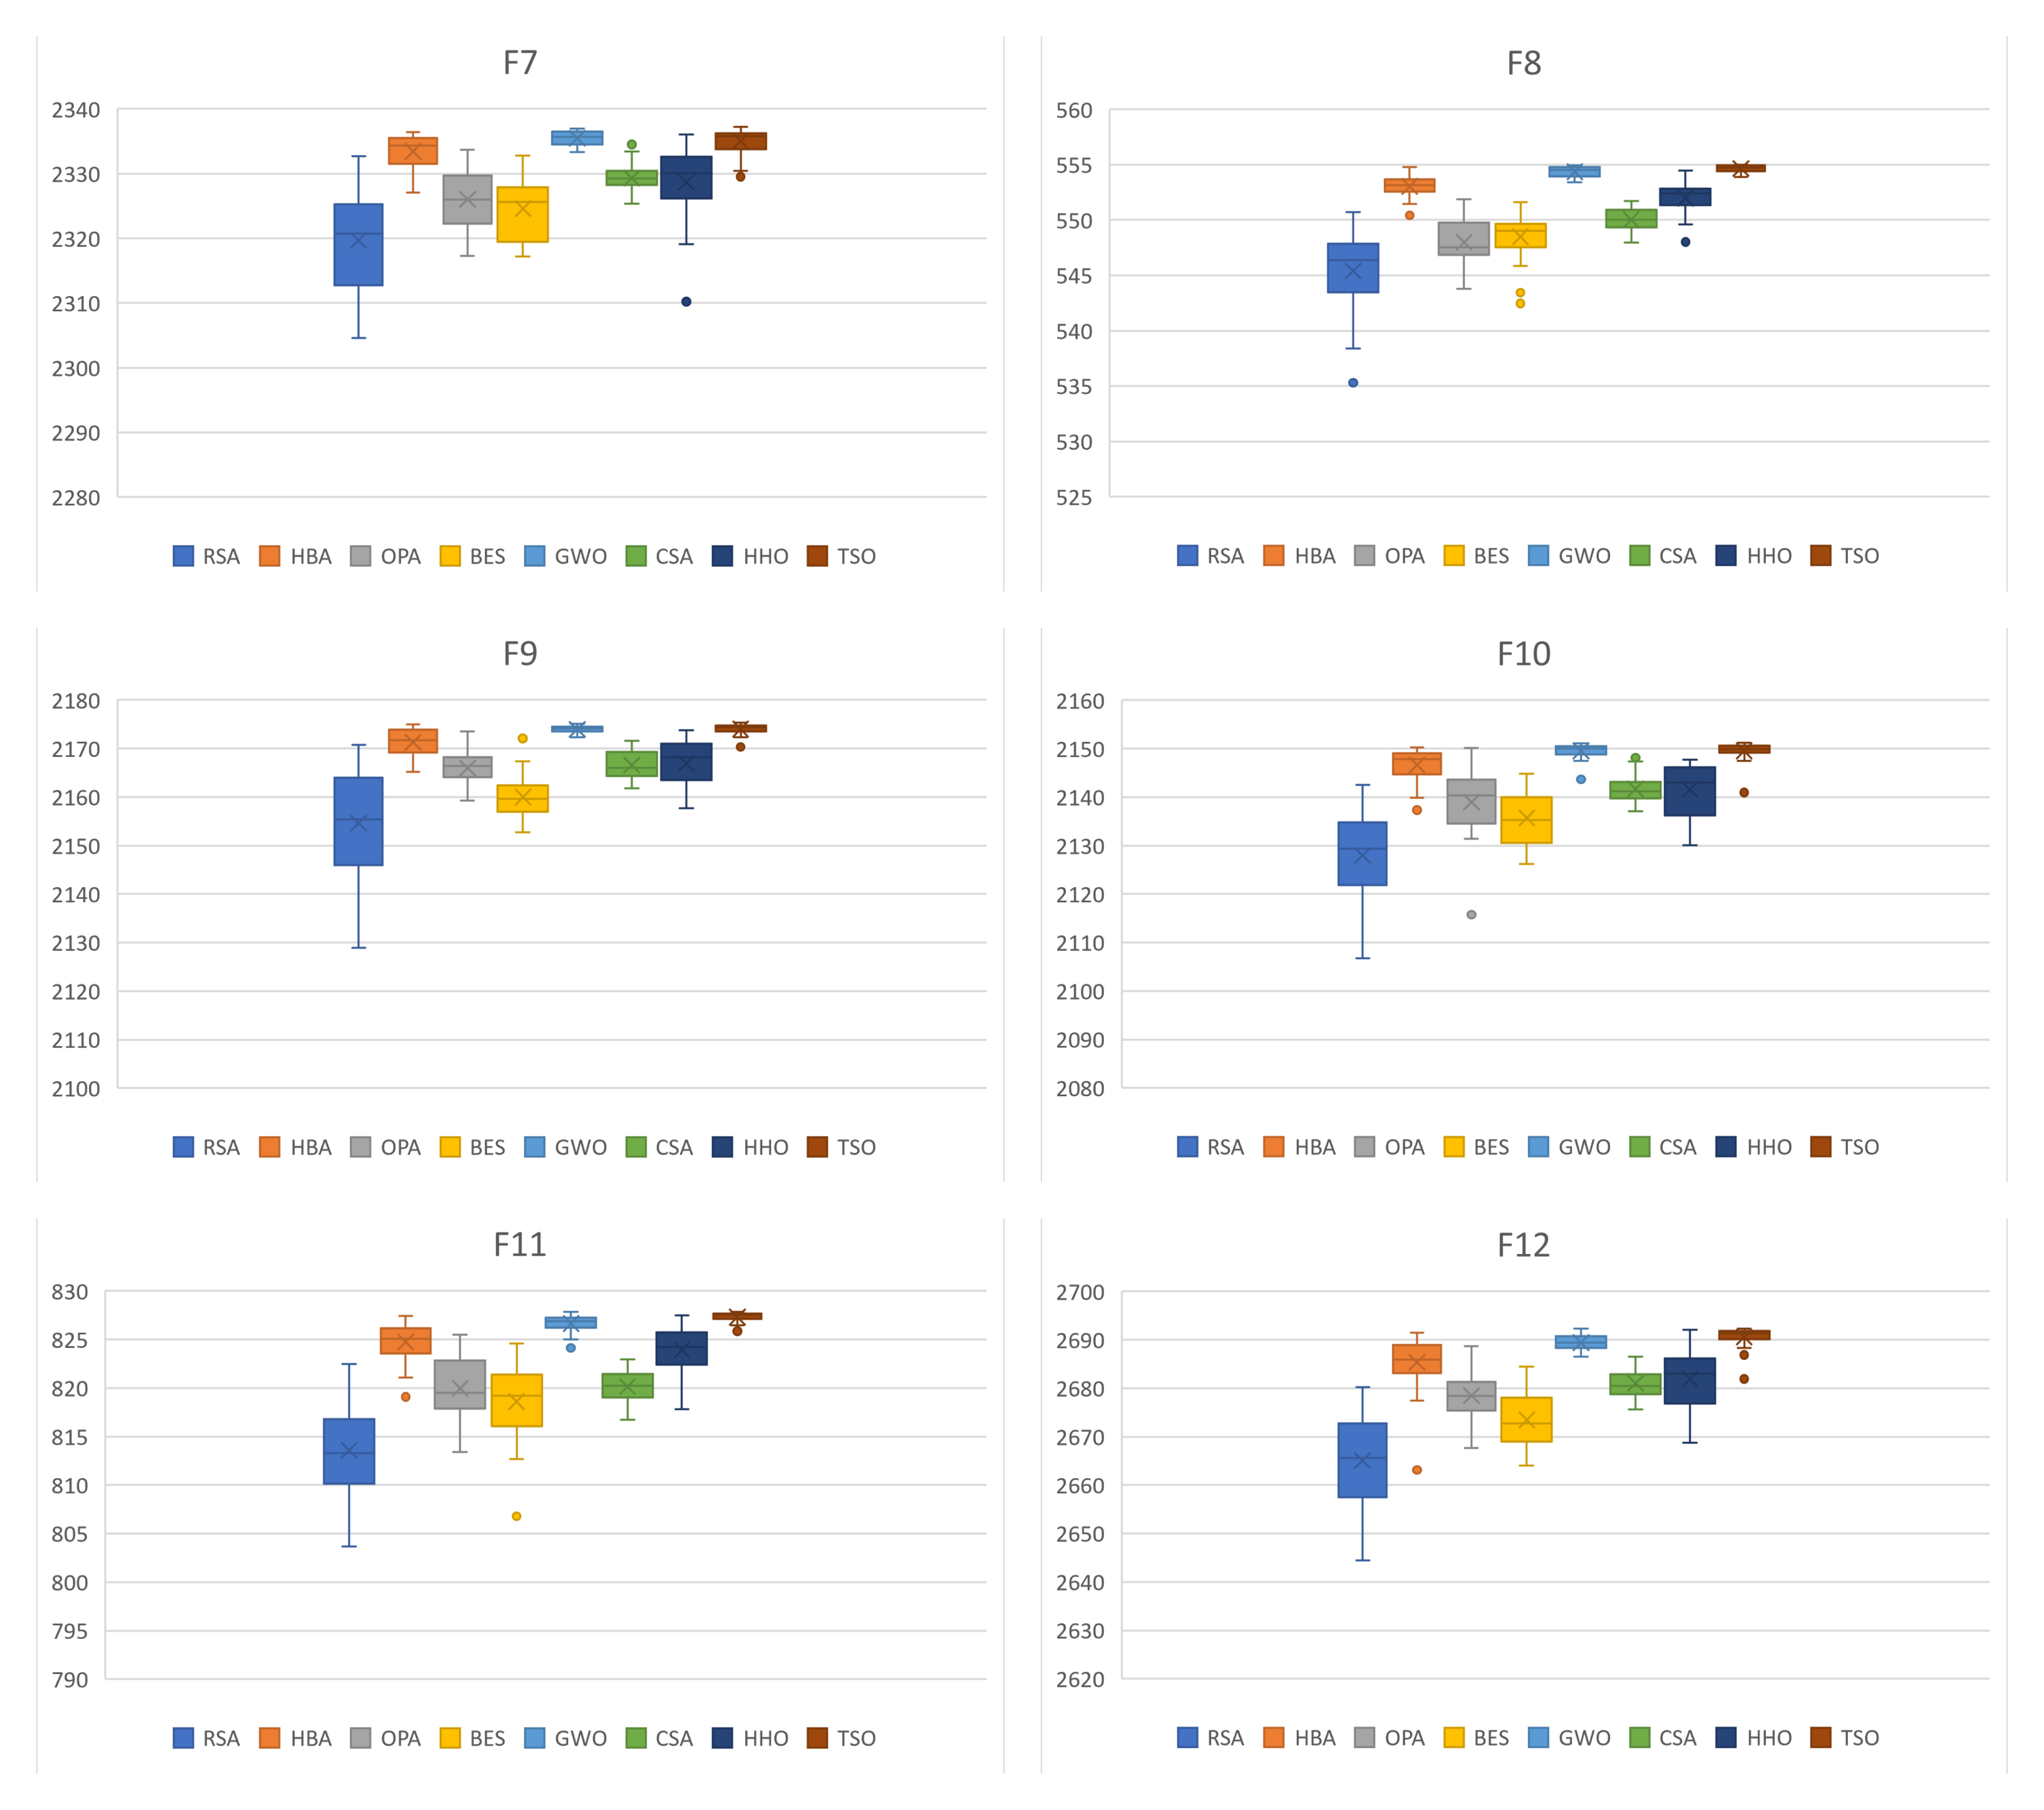
\includegraphics[width=\linewidth]{Fitness/Otsu/BoxPlot_Dim8/BoxPlots_7-12_Dim8.png}
	\end{subfigure}
	\begin{subfigure}{0.4\textwidth}
		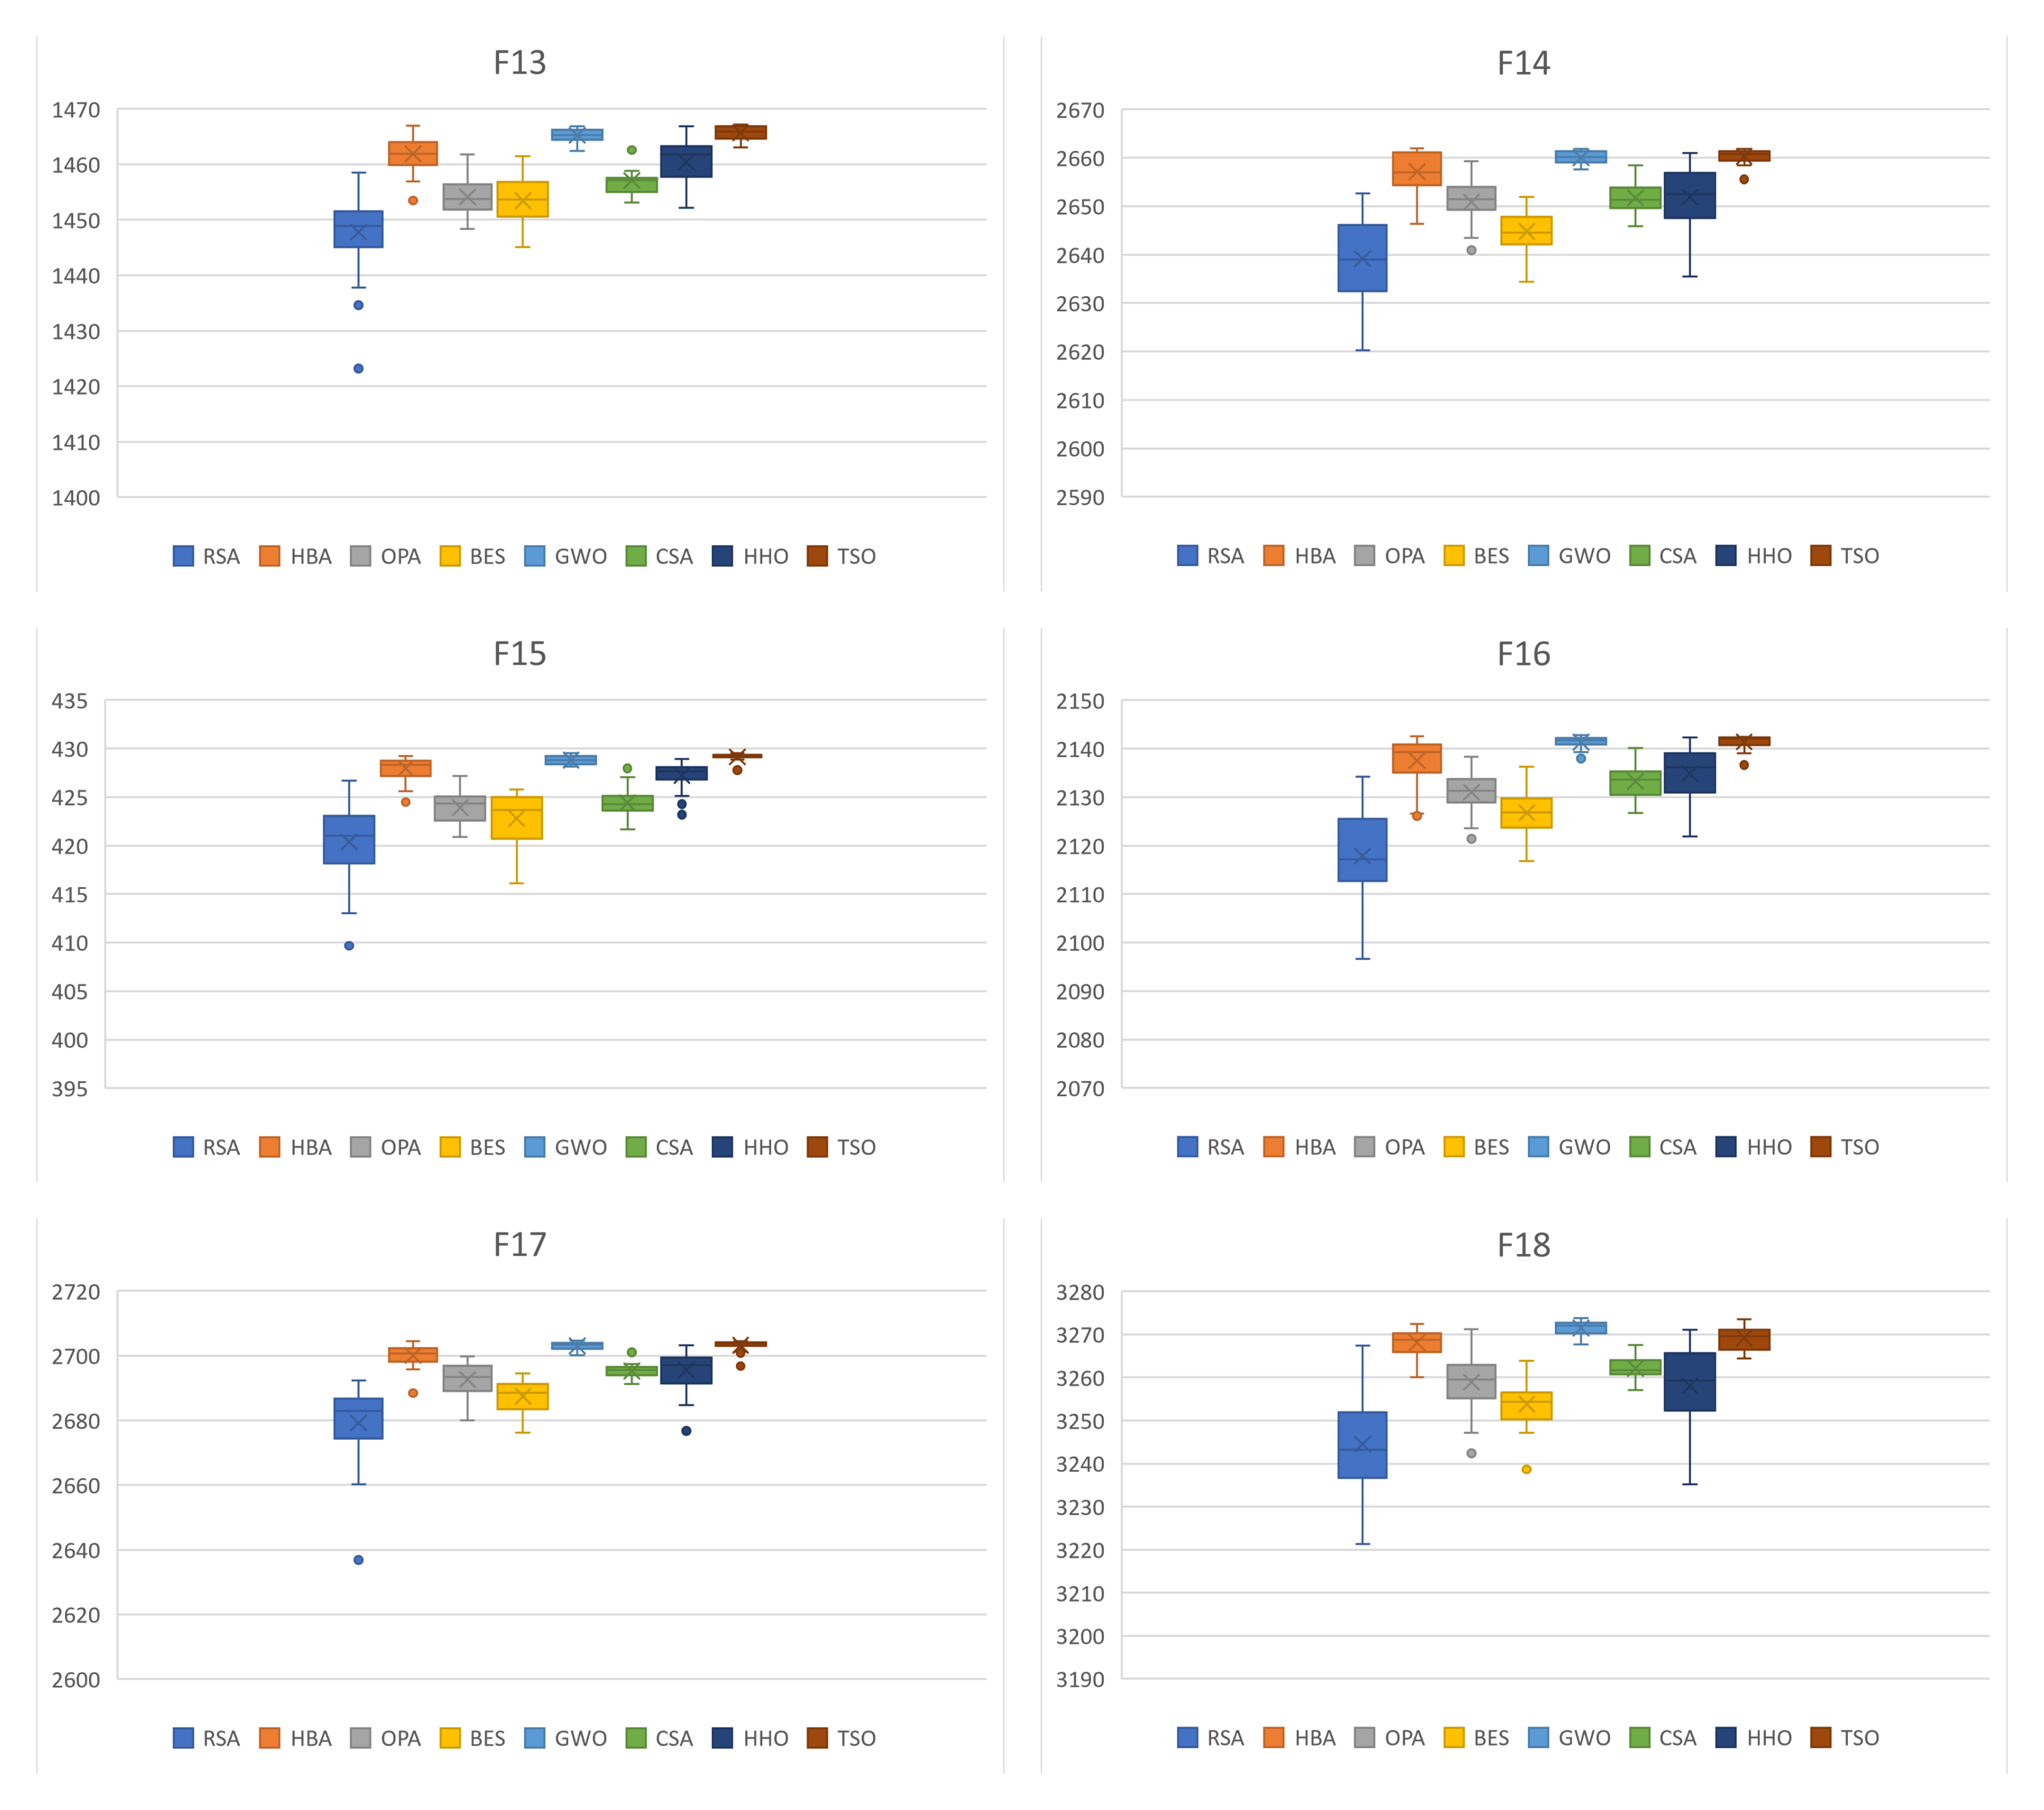
\includegraphics[width=\linewidth]{Fitness/Otsu/Boxplot_Dim8/BoxPlots_13-18_Dim8.png}
	\end{subfigure}
	\begin{subfigure}{0.4\textwidth}
		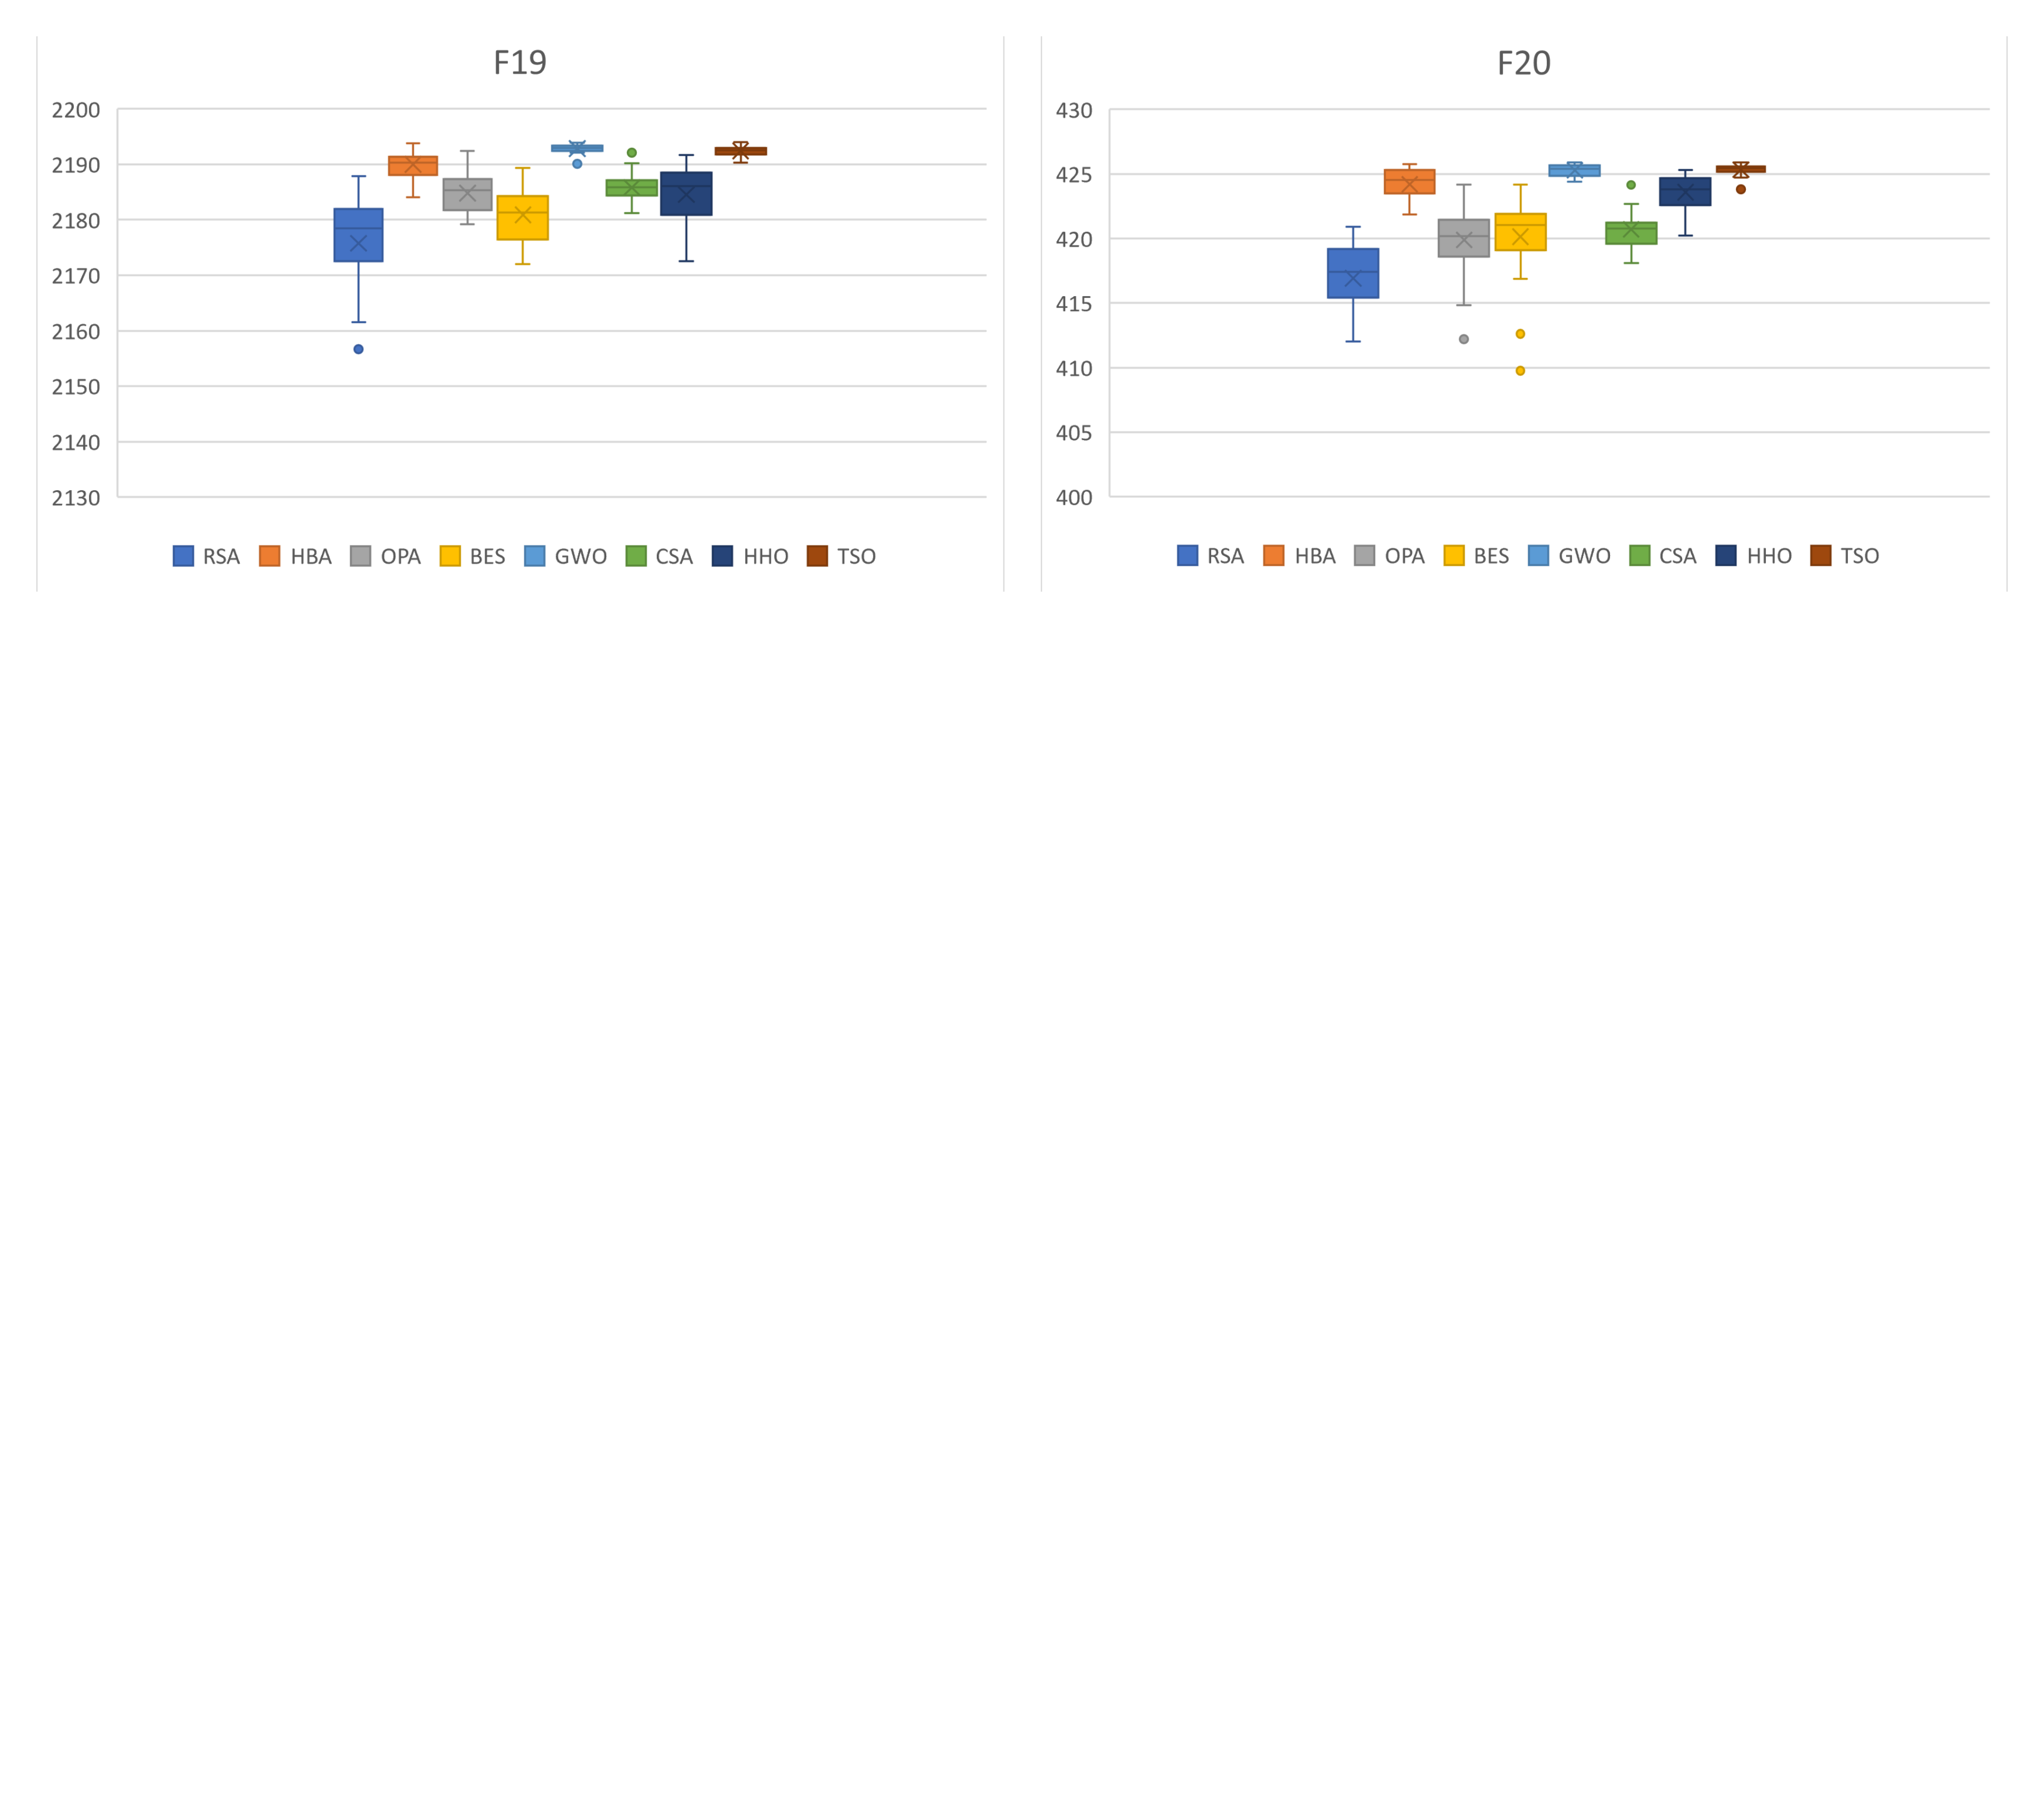
\includegraphics[width=\linewidth]{Fitness/Otsu/Boxplot_Dim8/BoxPlots_19-20_Dim8.png}
		\vspace{-120pt} % Ajusta este valor según sea necesario
	\end{subfigure}
	\caption{Boxplot de los valores Fitness por cada imagen en la dimensión 8, desde la imagen 1 hasta la imagen 20,Función Objetivo Otsu}
	\label{fig:imagenes}    
\end{figure}
\subsubsection{Dimensión 9}
\begin{itemize}
	\item GWO ha mostrado un rendimiento sobresaliente a través de las diferentes figuras. Posee una mediana consistentemente alta y una variabilidad baja, lo cual indica un rendimiento eficaz y consistente en la segmentación de imágenes.
	
	\item Algoritmos como CSA y TSO han mostrado resultados buenos y consistentes en varias figuras, pero con un rango de rendimiento que generalmente se encuentra entre el mejor y el peor, indicando un rendimiento medio.
	HBA y OPA también se encuentran en esta categoría, ya que no han tenido la consistencia o los valores de mediana más altos de GWO, pero aún así han superado a los algoritmos de peor rendimiento.
	Peor rendimiento:
	
	\item El RSA ha demostrado tener el peor rendimiento en la mayoría de las figuras analizadas, con la mediana más baja y una mayor variabilidad en los resultados.
	
\end{itemize}
% Dimension 9
\begin{figure}
	\centering
	
	\begin{subfigure}{0.4\textwidth}
		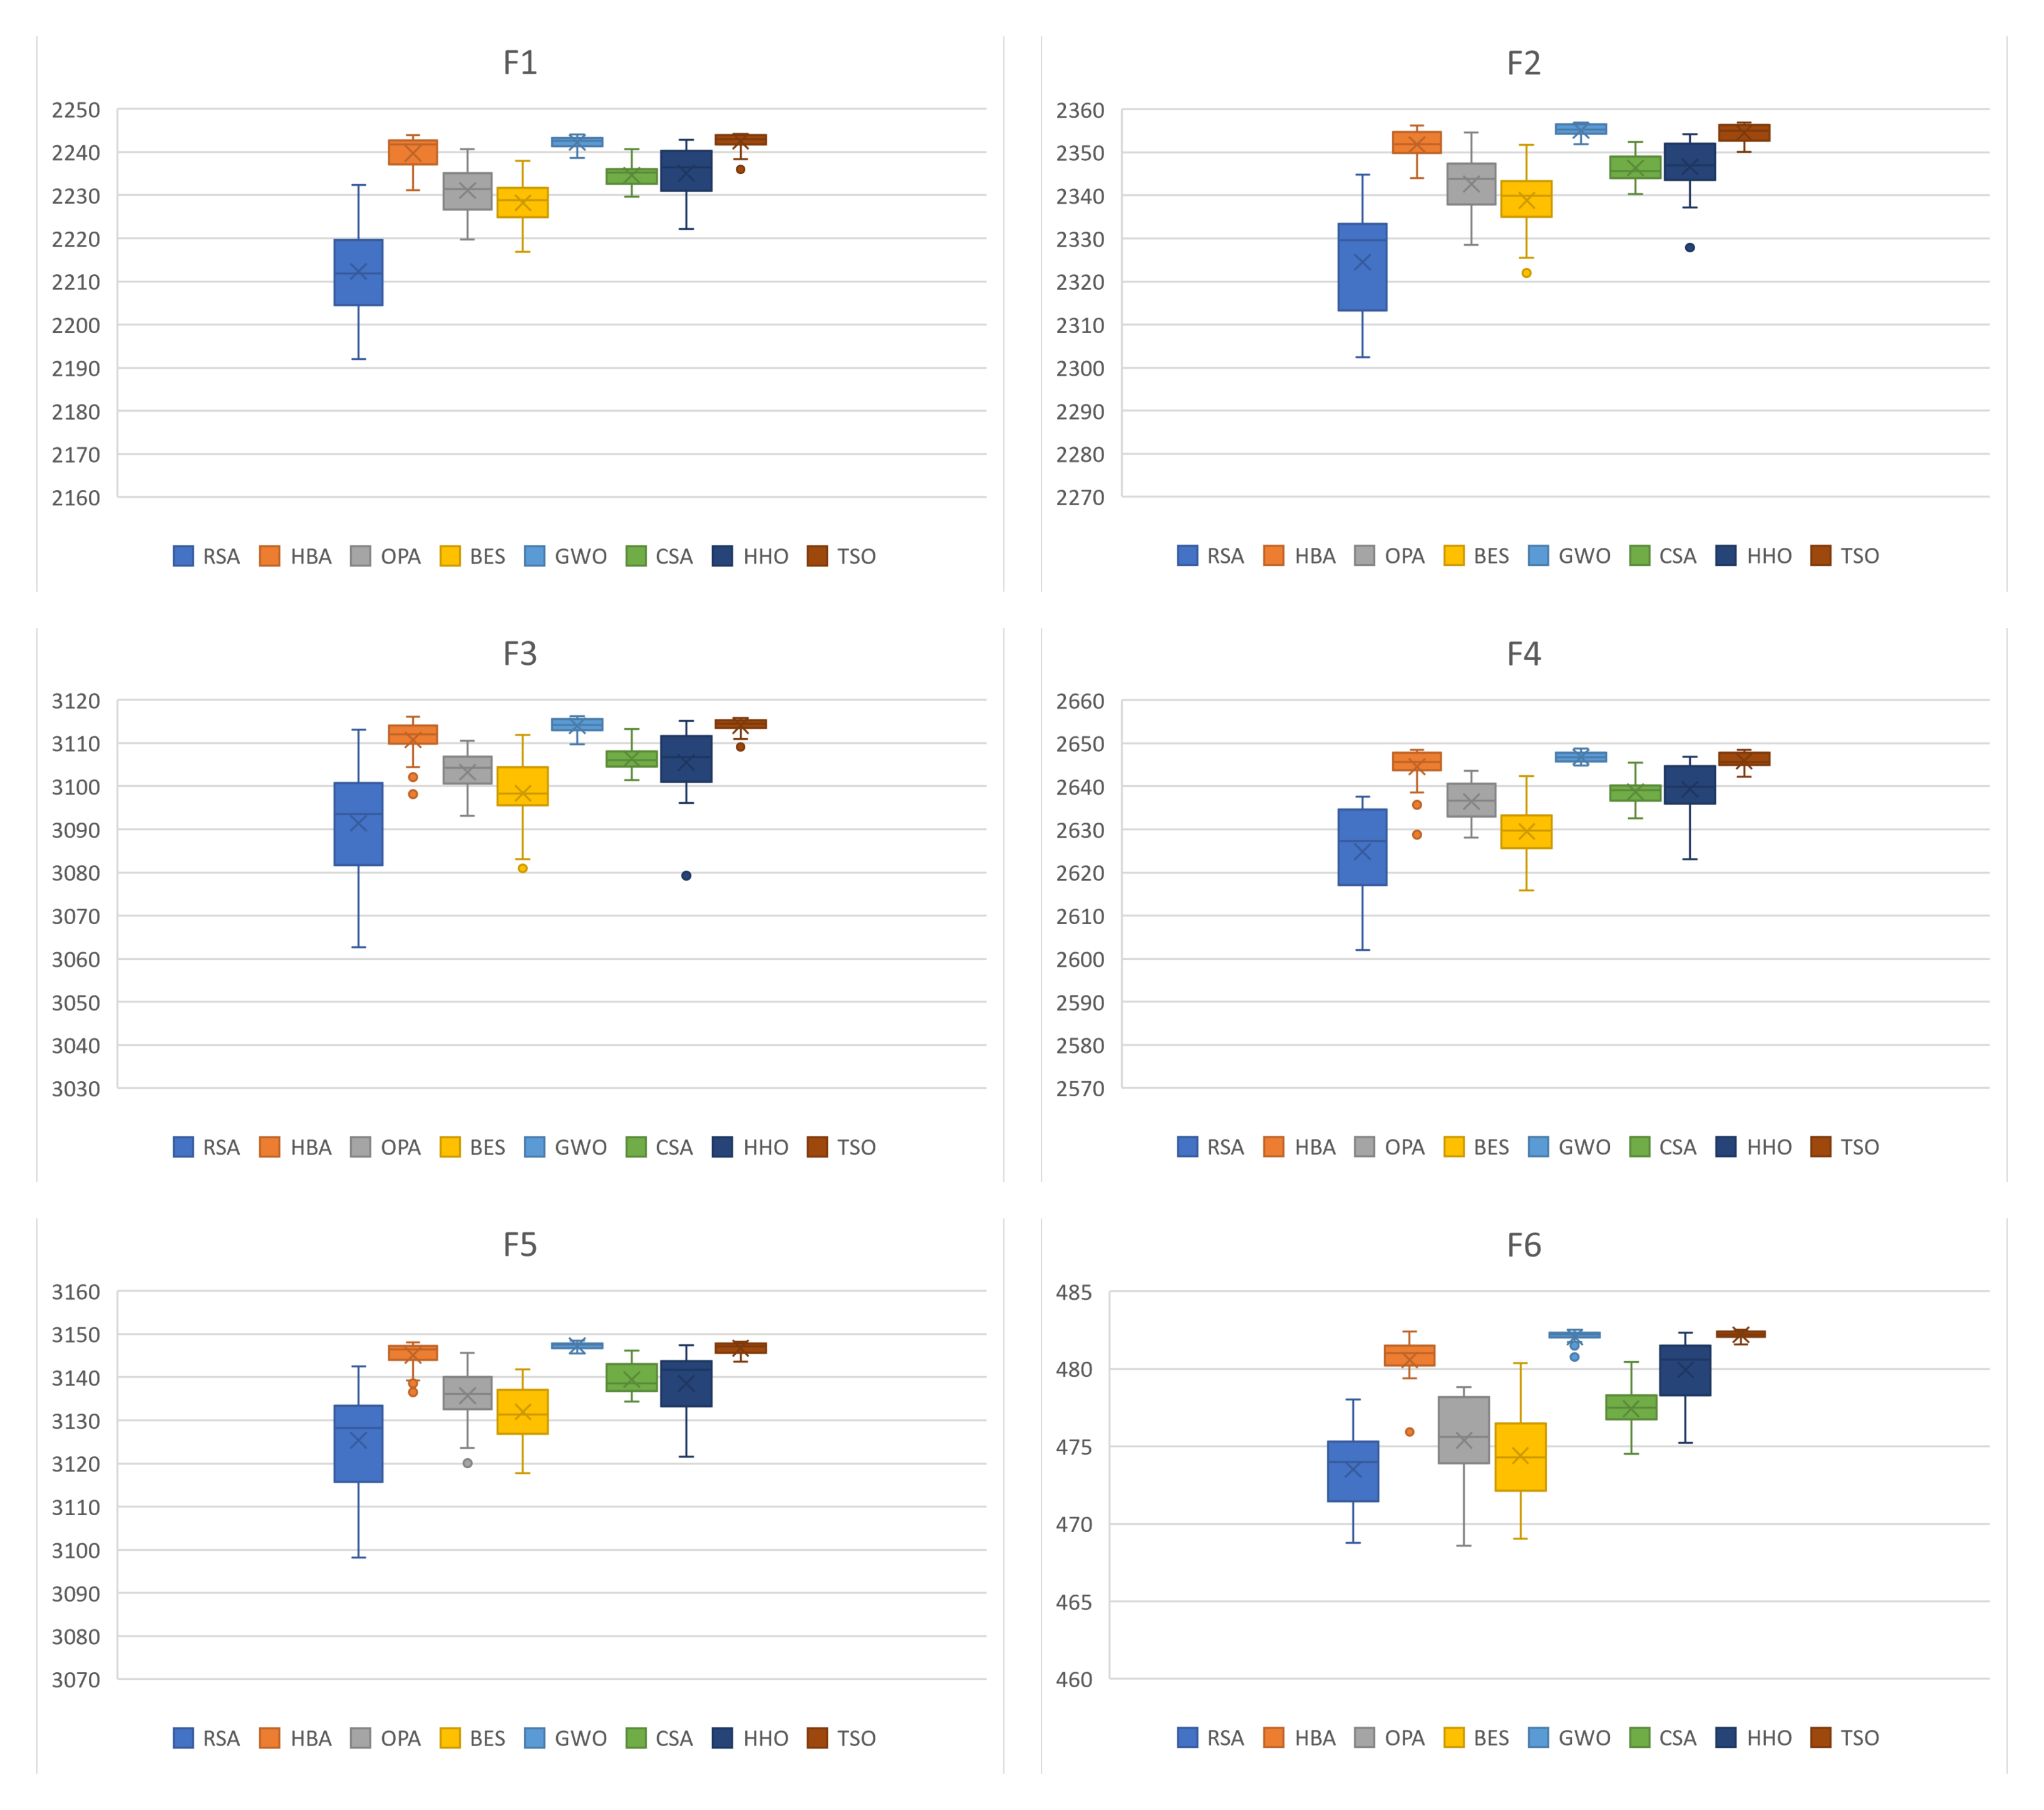
\includegraphics[width=\linewidth]{Fitness/Otsu/Boxplot_Dim9/BoxPlots_1-6_Dim9.png}
	\end{subfigure}
	
	\begin{subfigure}{0.4\textwidth}
		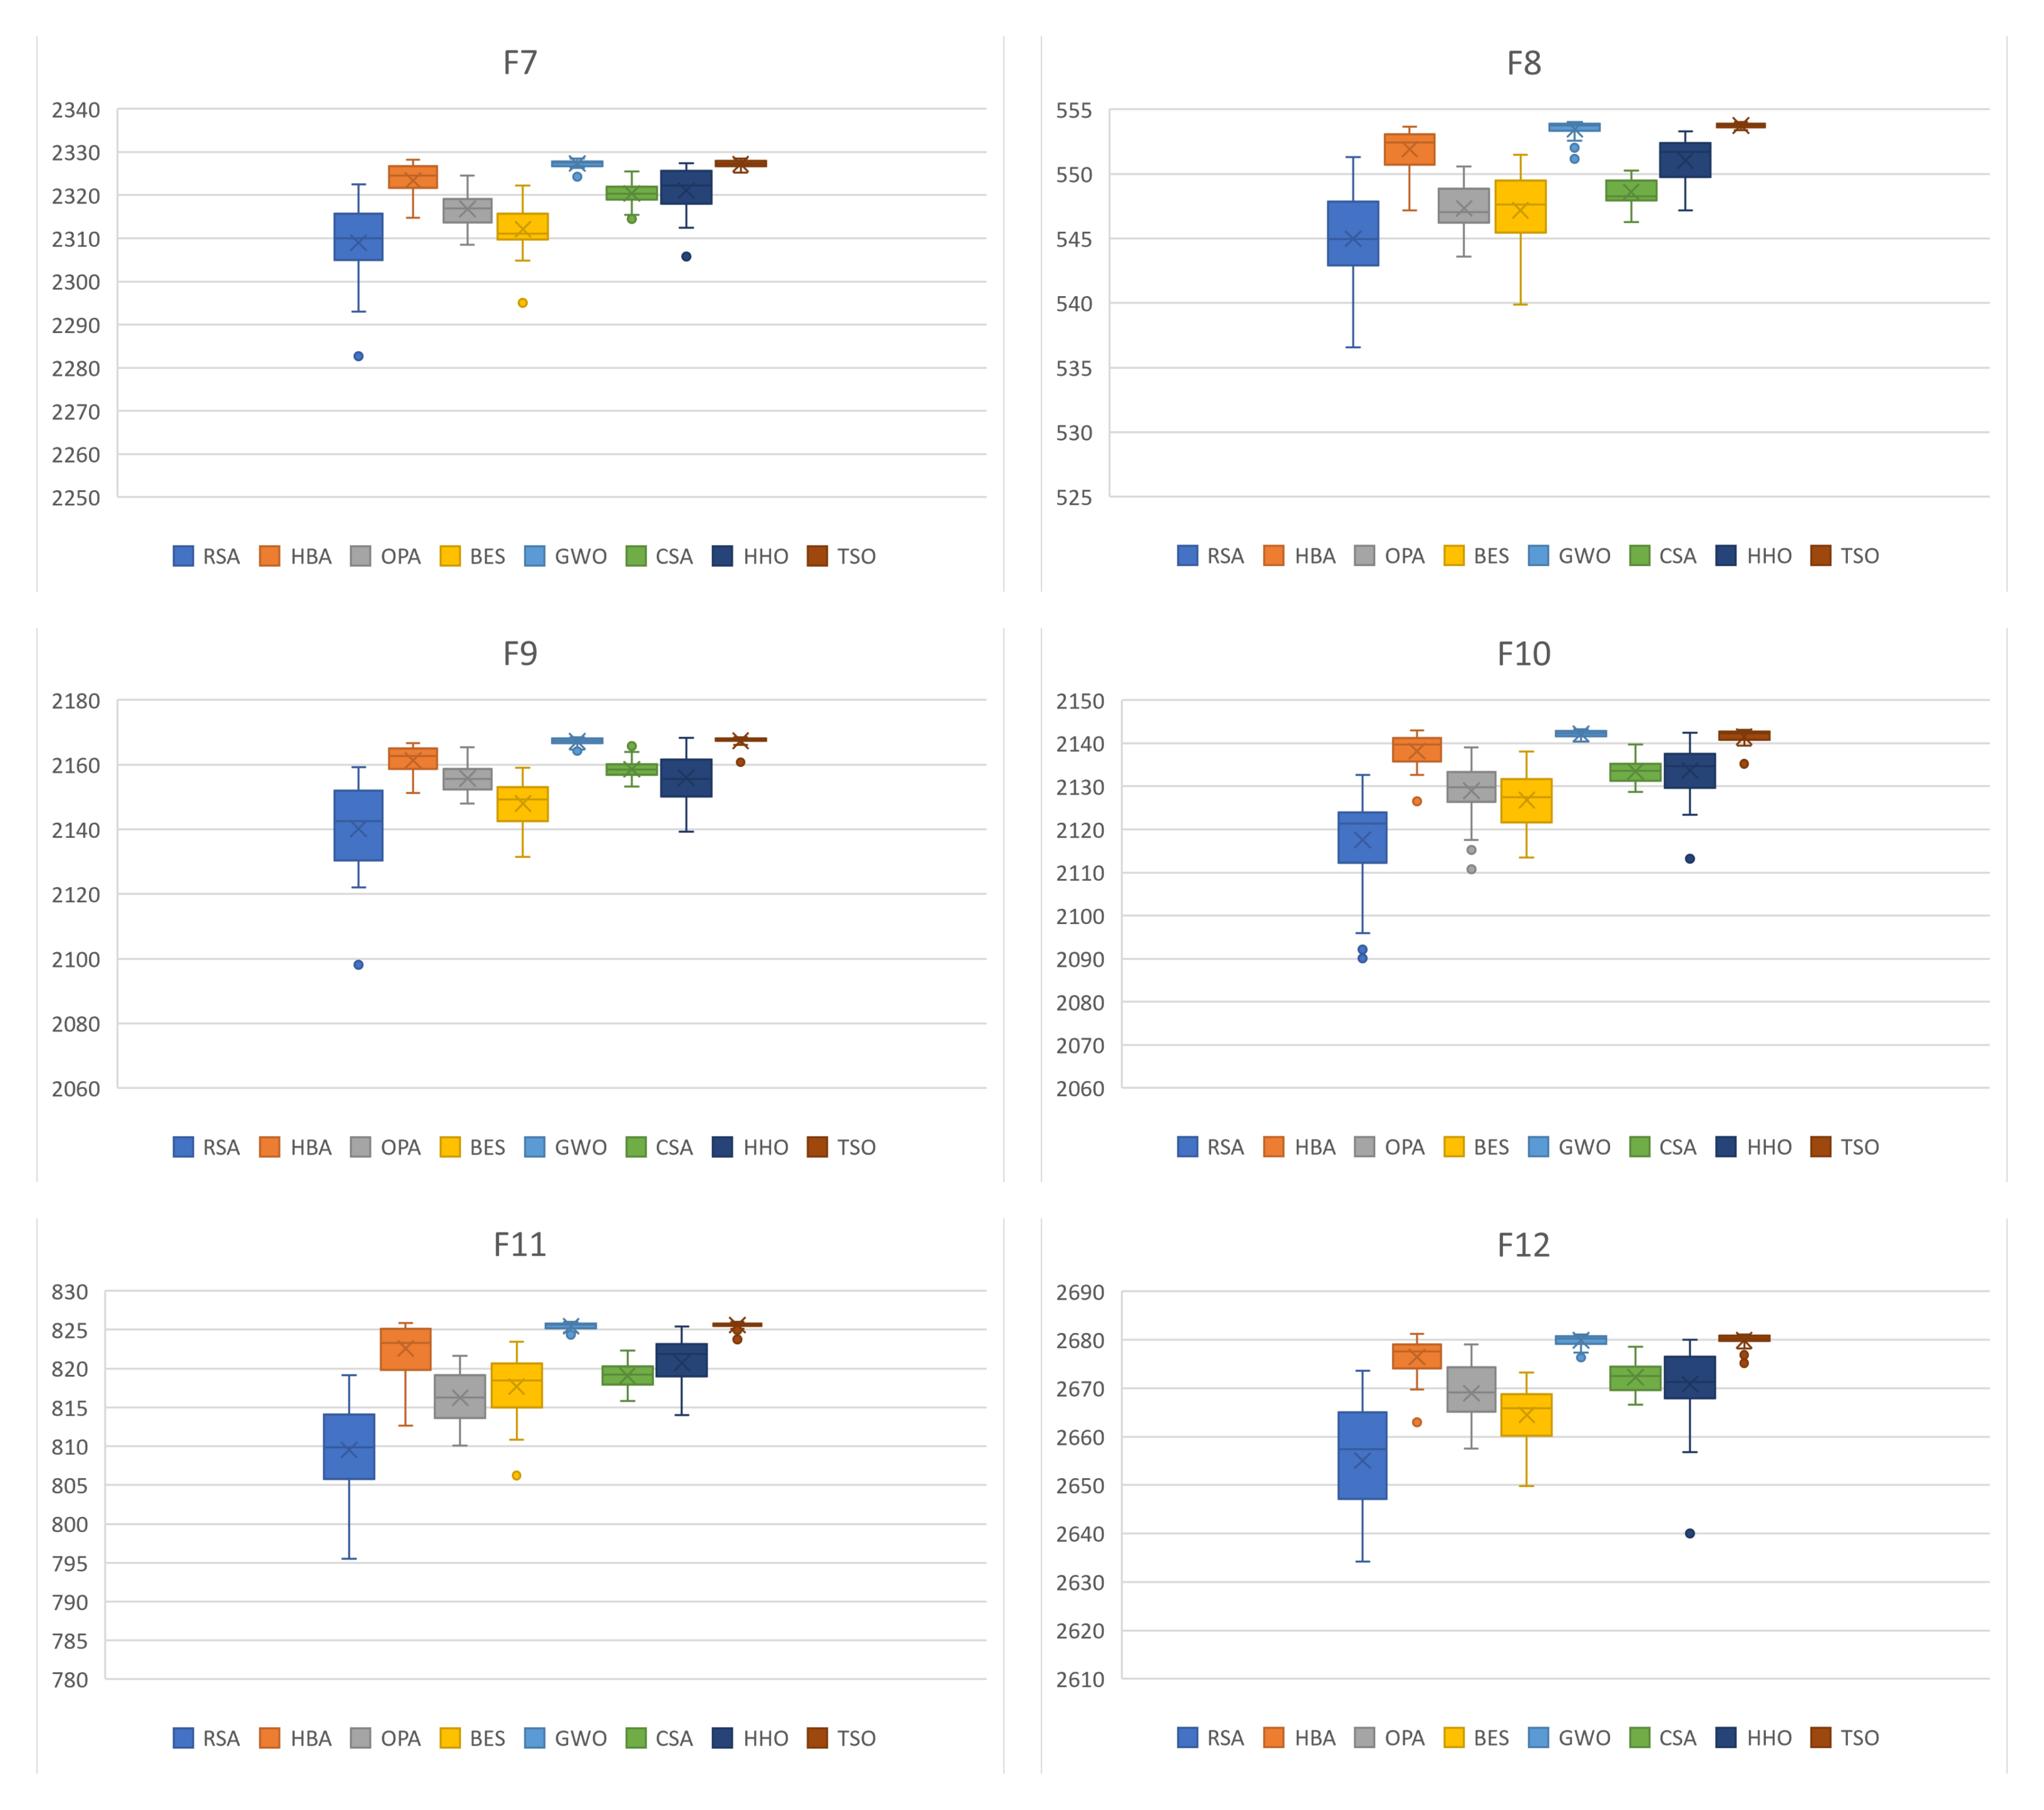
\includegraphics[width=\linewidth]{Fitness/Otsu/Boxplot_Dim9/BoxPlots_7-12_Dim9.png}
	\end{subfigure}
	\begin{subfigure}{0.4\textwidth}
		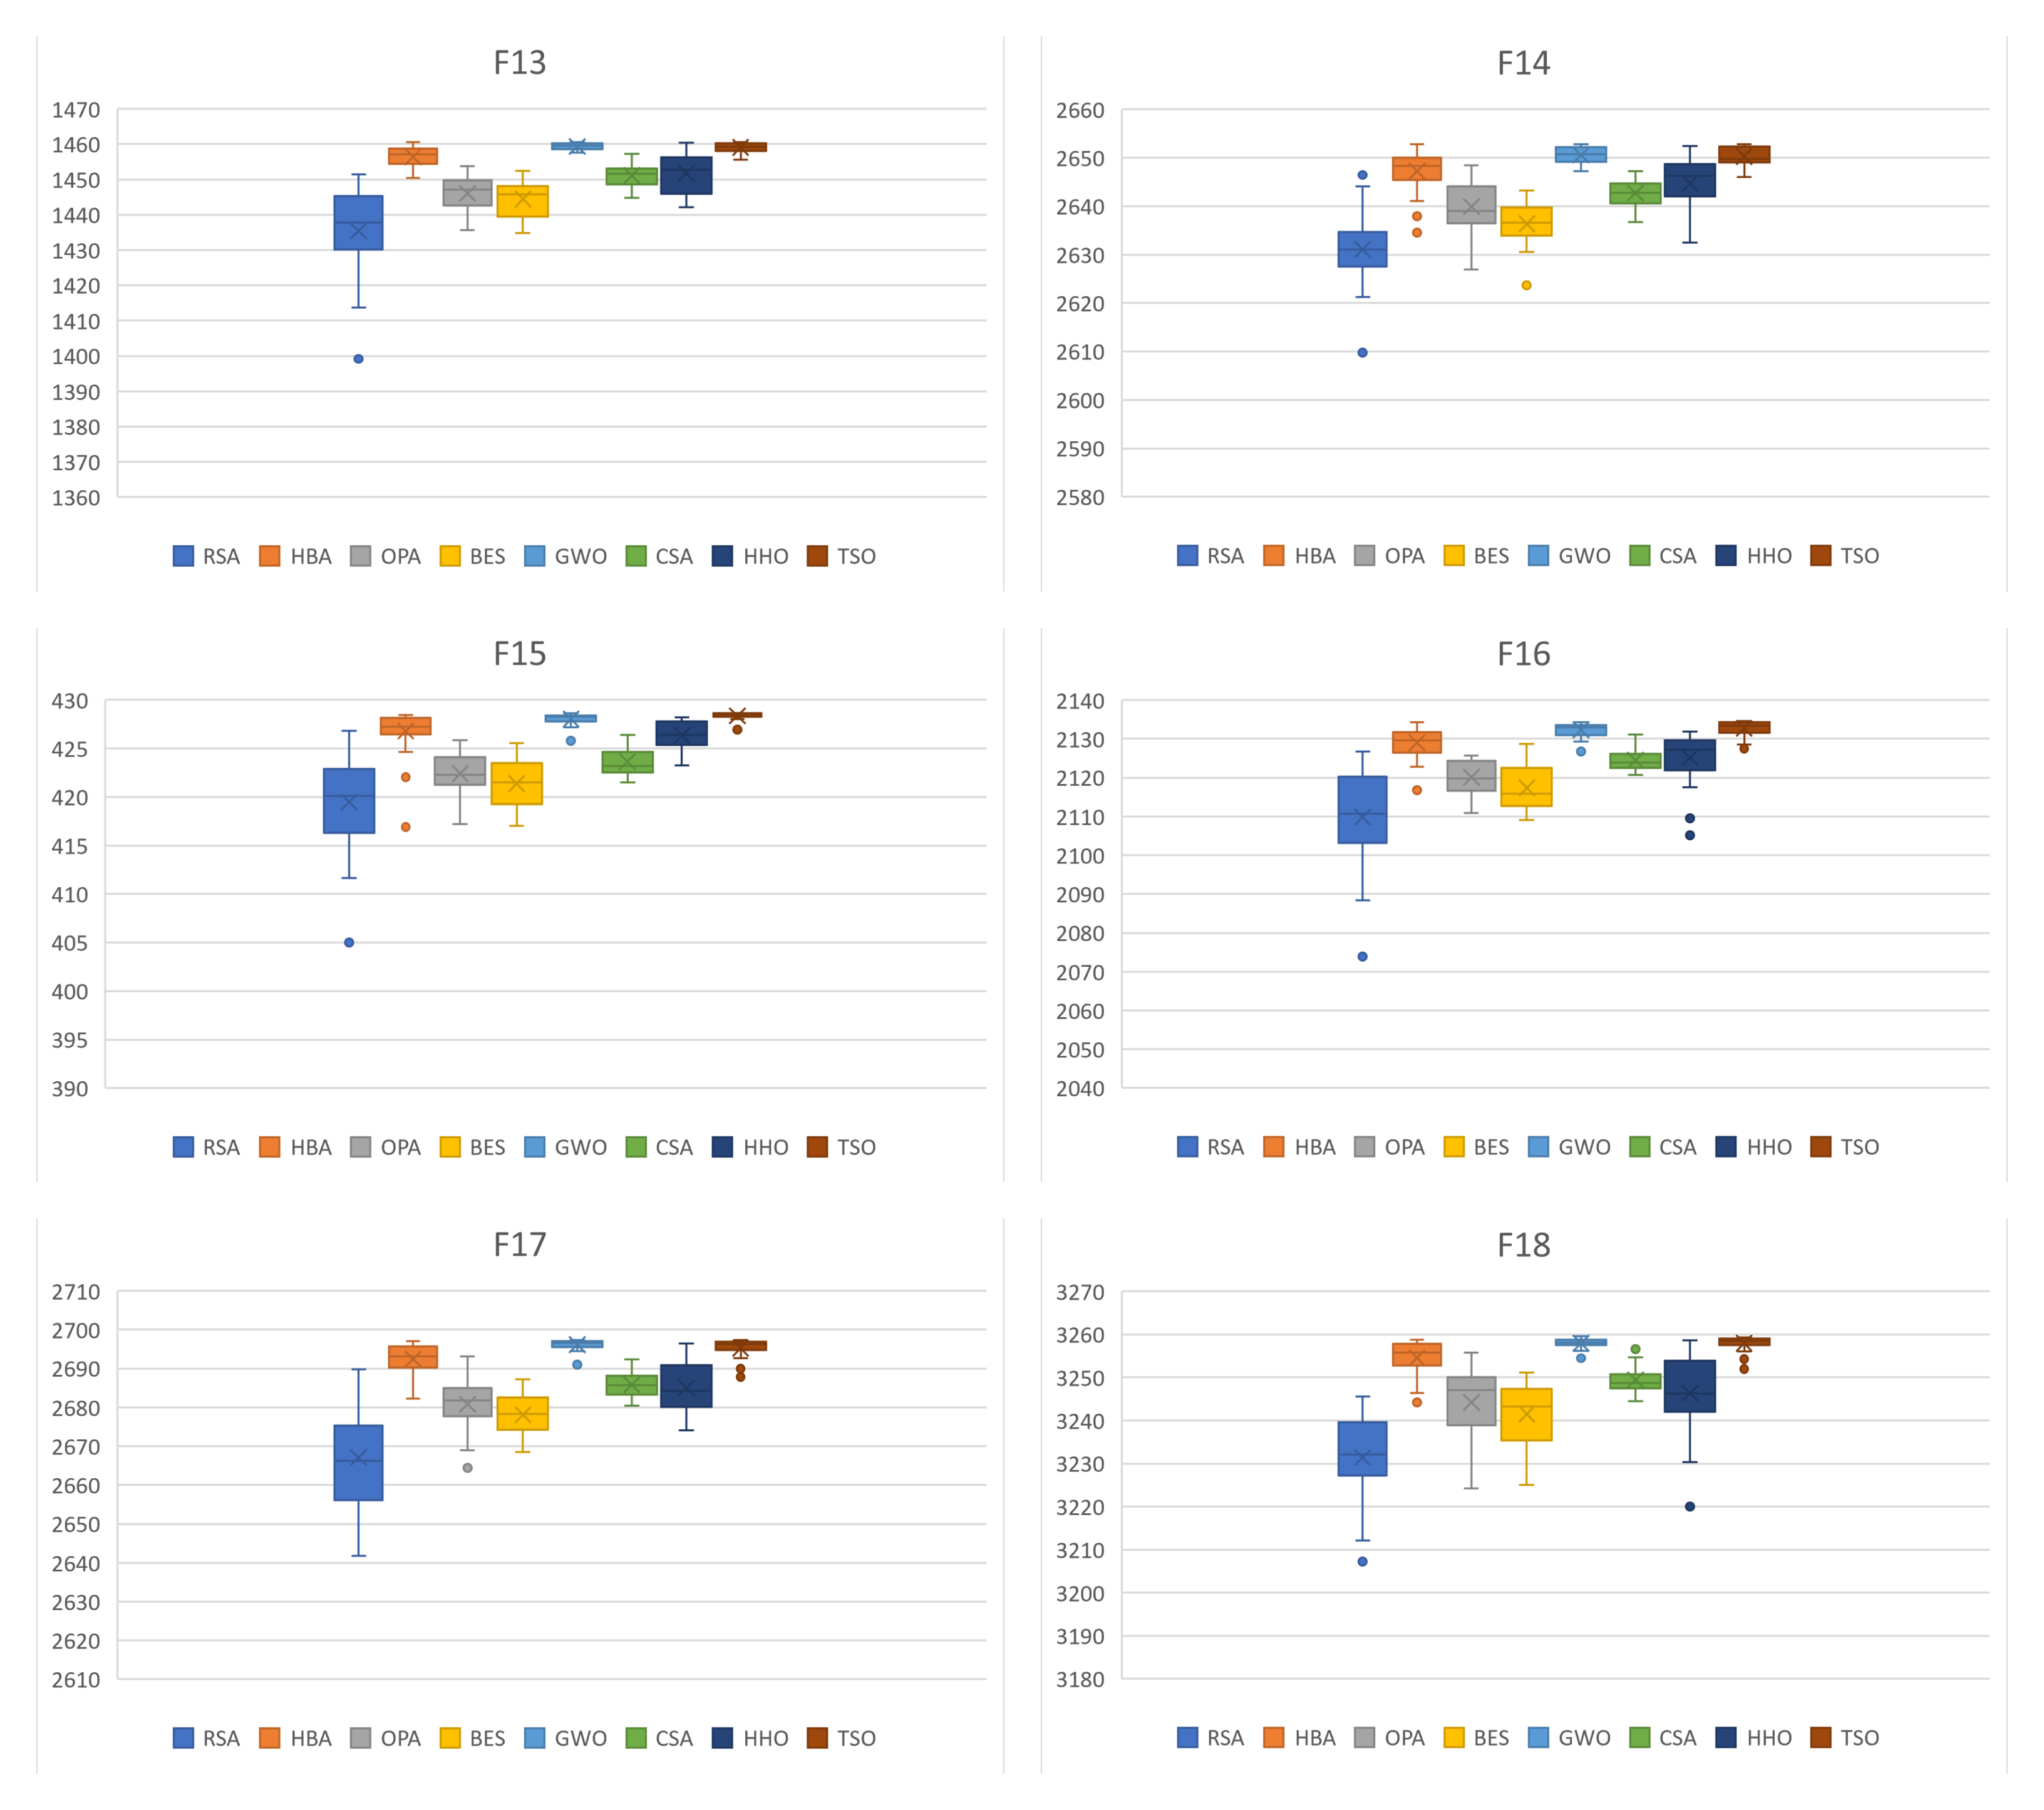
\includegraphics[width=\linewidth]{Fitness/Otsu/Boxplot_Dim9/BoxPlots_13-18_Dim9.png}
	\end{subfigure}
	\begin{subfigure}{0.4\textwidth}
		\includegraphics[width=\linewidth]{Fitness/Otsu/Boxplot_Dim9/BoxPlots_19-20_Dim9.png}
		\vspace{-120pt} % Ajusta este valor según sea necesario
	\end{subfigure}
	\caption{Boxplot de los valores Fitness por cada imagen en la dimensión 9, desde la imagen 1 hasta la imagen 20,Función Objetivo Otsu}
	\label{fig:imagenes}    
\end{figure}

\subsection{Resultados Función PSNR Otsu}
\subsubsection{Dimensión 7}
\begin{itemize}
\item El RSA muestra una mediana en un nivel medio comparado con los demás algoritmos y un rango intercuartílico estrecho, lo que sugiere consistencia en la calidad de las imágenes.
Sin embargo, la presencia de valores atípicos altos sugiere que en algunas instancias, puede alcanzar una calidad excepcionalmente alta.

\item HBA tiene una mediana ligeramente superior a la de RSA, indicando un rendimiento medio en general. No obstante, su rango intercuartílico es más amplio y tiene varios valores atípicos en el extremo inferior, lo que puede indicar una menor consistencia en comparación con RSA.
\item OPA presenta una mediana comparable a la de HBA, pero con un rango intercuartílico más amplio, lo que indica una mayor variabilidad en la calidad de reconstrucción de las imágenes. Los valores atípicos bajos sugieren que puede haber instancias de rendimiento significativamente peor.

\item BES tiene la mediana más baja entre los primeros cuatro algoritmos, con un rango intercuartílico muy amplio, lo que indica una alta variabilidad en la calidad de las imágenes. La presencia de un valor atípico muy alto indica que bajo ciertas condiciones podría alcanzar una calidad muy alta, aunque estos casos parecen ser excepcionales.

\item El algoritmo GWO muestra una mediana que está entre las más altas y un IQR estrecho, lo que sugiere una buena consistencia en la calidad de reconstrucción de las imágenes. La ausencia de valores atípicos indica que su rendimiento es predecible y confiable.

\item CSA presenta resultados muy similares a GWO, con una mediana alta y un rango intercuartílico estrecho, lo que sugiere un rendimiento consistente y confiable. La presencia de un único valor atípico bajo no afecta significativamente su evaluación general.

\item HHO tiene una mediana más baja comparada con GWO y CSA, y un rango intercuartílico mediano. Esto sugiere un rendimiento generalmente bueno pero con una variabilidad más alta que los líderes (GWO y CSA).
\item TSO tiene la mediana más baja de todos, lo que indica el rendimiento más bajo en términos de calidad de imagen. A pesar de tener un rango intercuartílico estrecho, los valores atípicos altos sugieren que puede haber casos aislados de buen rendimiento, pero no son suficientes para elevar su evaluación general.
\end{itemize}

\noindent En general el mejor rendimiento: GWO y CSA son los algoritmos con el mejor rendimiento, mostrando medianas altas y consistencia en los resultados del PSNR, mientras que RSA, HBA y OPA tienen un rendimiento medio con una variabilidad más alta en sus resultados y BES y TSO se encuentran en el extremo inferior de rendimiento, con TSO como el que tiene el rendimiento más bajo debido a su baja mediana de PSNR. BES, aunque tiene un rendimiento medio-bajo, tiene la posibilidad de alcanzar resultados altos de forma atípica.
% Dimension 7 PSNR OTSU
\begin{figure}
	\centering
	\begin{subfigure}{0.4\textwidth}
		\includegraphics[width=\linewidth]{PSNR/Otsu/Dim7/PSNR_Dim7_Otsu_1_6.png}
	\end{subfigure}
	
	\begin{subfigure}{0.4\textwidth}
		\includegraphics[width=\linewidth]{PSNR/Otsu/Dim7/PSNR_Dim7_Otsu_7_12.png}
	\end{subfigure}
	\begin{subfigure}{0.4\textwidth}
		\includegraphics[width=\linewidth]{PSNR/Otsu/Dim7/PSNR_Dim7_Otsu_13_18.png}
	\end{subfigure}
	\begin{subfigure}{0.4\textwidth}
		\includegraphics[width=\linewidth]{PSNR/Otsu/Dim7/PSNR_Dim7_Otsu_19_20.png}
		\vspace{-120pt} % Ajusta este valor según sea necesario
	\end{subfigure}
	\caption{Boxplot de los valores PSNR por cada imagen en la dimensión 7, desde la imagen 1 hasta la imagen 20,Función Objetivo Otsu}
	\label{fig:imagenes}    
\end{figure}
\subsubsection{Dimensión 8}
\begin{itemize}
\item RSA la mediana está por debajo de 20, con varios valores atípicos por encima de la caja. La variabilidad es considerable, indicada por el rango intercuartílico (la altura de la caja) y los bigotes extensos. Esto sugiere que el RSA tiene un rendimiento inconsistente.

\item HBA con una mediana ligeramente superior a la del RSA y menos valores atípicos. La caja y los bigotes indican una variabilidad similar al RSA. La presencia de valores atípicos hacia abajo sugiere que el HBA puede tener casos donde el rendimiento es significativamente peor que el promedio.

\item OPA tiene una mediana cercana a 20 y una variabilidad moderada, con menos valores atípicos que RSA y HBA. Esto indica un rendimiento más consistente pero aún con fluctuaciones.

\item BES presenta la mediana más baja, lo que sugiere un rendimiento promedio inferior. Tiene una alta variabilidad y el mayor número de valores atípicos, lo que indica que su rendimiento puede ser bastante impredecible.

\item GWO se observa una mediana alrededor de los 20 con una de las variabilidades más bajas y sin valores atípicos, lo que sugiere que GWO tiene un rendimiento consistente y predecible.

\item CSA presenta una mediana similar a GWO y también una baja variabilidad, lo que indica un rendimiento consistente. Tiene un valor atípico, pero en general parece ser una opción confiable.

\item HHO con una mediana en el mismo rango que GWO y CSA, y una variabilidad ligeramente mayor, el HHO sigue siendo un algoritmo con buen rendimiento. La presencia de valores atípicos indica que puede tener casos de rendimiento tanto muy buenos como malos.

\item TSO a pesar de tener la media y la mediana más alta, se observa que tiene una variabilidad significativa, lo que indica que mientras que algunos de sus resultados son muy buenos, otros pueden ser mucho más bajos. La presencia de un valor atípico extremo hacia abajo sugiere que en ciertos casos, su rendimiento puede ser considerablemente peor que el promedio.
\end{itemize}
\noindent Al revisar detenidamente, los algoritmos GWO, CSA y HHO muestran un rendimiento más consistente y predecible que TSO, a pesar de que este último tiene valores máximos más altos. Esto se debe a su variabilidad comparativamente alta y presencia de valores atípicos. Para aplicaciones donde la consistencia es tan importante como la calidad máxima, GWO, CSA y HHO pueden ser preferibles. BES, con la variabilidad más alta y la mediana más baja, parece ser el menos deseable. La elección del algoritmo debería basarse en el equilibrio entre la calidad promedio deseada de la reconstrucción de imagen y la tolerancia a la variabilidad en los resultados.
% Dimension 8 PSNR OTSU
\begin{figure}
	\centering
	\begin{subfigure}{0.4\textwidth}
		\includegraphics[width=\linewidth]{PSNR/Otsu/Dim8/PSNR_Dim8_Otsu_1_6.png}
	\end{subfigure}
	
	\begin{subfigure}{0.4\textwidth}
		\includegraphics[width=\linewidth]{PSNR/Otsu/Dim8/PSNR_Dim8_Otsu_7_12.png}
	\end{subfigure}
	\begin{subfigure}{0.4\textwidth}
		\includegraphics[width=\linewidth]{PSNR/Otsu/Dim8/PSNR_Dim8_Otsu_13_18.png}
	\end{subfigure}
	\begin{subfigure}{0.4\textwidth}
		\includegraphics[width=\linewidth]{PSNR/Otsu/Dim8/PSNR_Dim8_Otsu_19_20.png}
		\vspace{-120pt} % Ajusta este valor según sea necesario
	\end{subfigure}
	\caption{Boxplot de los valores PSNR por cada imagen en la dimensión 8, desde la imagen 1 hasta la imagen 20,Función Objetivo Otsu}
	\label{fig:imagenes}    
\end{figure}

\subsubsection{Dimensión 9}
\begin{itemize}
\item RSA tiende a una variabilidad moderada. Esto sugiere un rendimiento generalmente confiable y consistente en diferentes imágenes.
\item HBA Muestra una mediana ligeramente variable, generalmente en el rango medio bajo, Su rendimiento es menos consistente que el de RSA.
\item OPA presenta medianas similares a las de HBA, con variabilidades moderadas a altas y algunos valores atípicos. Esto indica un rendimiento medio con cierta inconsistencia.
\item BES tiene las medianas más bajas y alta variabilidad en todos los conjuntos de datos, lo que indica un rendimiento generalmente inferior y poco fiable.
\item GWO muestra medianas consistentemente altas y variabilidades moderadas sin muchos valores atípicos. Esto sugiere que GWO es generalmente robusto y confiable.
\item CSA Tiene medianas altas y las variabilidades más bajas en la mayoría de los conjuntos de datos. CSA parece ofrecer el equilibrio más consistente entre calidad y fiabilidad.
\item HHO presenta un comportamiento similar a GWO y CSA, con medianas altas y variabilidad moderada a baja. Es otro algoritmo robusto y confiable.
\item TSO Aunque en un caso (F7) TSO mostró la mediana más alta, en general su rendimiento es muy variable, con la mayor dispersión en todos los conjuntos de datos. Esto indica que mientras tiene el potencial de lograr una alta calidad de reconstrucción, su rendimiento es inconsistente.
	
\end{itemize}
\noindent En General CSA y HHO parecen ser los más consistentes a través de los diferentes conjuntos de datos, ofreciendo un buen equilibrio entre alta calidad de reconstrucción y baja variabilidad.

\noindent Mejor rendimiento promedio GWO también ofrece un buen rendimiento, pero con ligeramente más variabilidad que CSA y HHO.

\noindent Inconsistencia TSO, a pesar de tener un buen rendimiento en algunos casos, es el más inconsistente, lo que puede ser problemático en aplicaciones donde la fiabilidad es crítica.

\noindent Menor rendimiento BES parece ser el menos confiable y el que tiene un rendimiento más bajo en promedio.
% Dimension 9 PSNR OTSU
\begin{figure}
	\centering
	\begin{subfigure}{0.4\textwidth}
		\includegraphics[width=\linewidth]{PSNR/Otsu/Dim9/PSNR_Dim9_Otsu_1_6.png}
	\end{subfigure}
	
	\begin{subfigure}{0.4\textwidth}
		\includegraphics[width=\linewidth]{PSNR/Otsu/Dim9/PSNR_Dim9_Otsu_7_12.png}
	\end{subfigure}
	\begin{subfigure}{0.4\textwidth}
		\includegraphics[width=\linewidth]{PSNR/Otsu/Dim9/PSNR_Dim9_Otsu_13_18.png}
	\end{subfigure}
	\begin{subfigure}{0.4\textwidth}
		\includegraphics[width=\linewidth]{PSNR/Otsu/Dim9/PSNR_Dim9_Otsu_19_20.png}
		\vspace{-120pt} % Ajusta este valor según sea necesario
	\end{subfigure}
	\caption{Boxplot de los valores PSNR por cada imagen en la dimensión 9, desde la imagen 1 hasta la imagen 20,Función Objetivo Otsu}
	\label{fig:imagenes}    
\end{figure}

\subsection{Resultados Función SSIM Otsu}
\subsubsection{Dimensión 7}
\begin{itemize}
\item TSO: Mostró un buen rendimiento, lo cual sugiere que es el mejor algoritmo en esta métrica. Sin embargo, para F6, TSO fue uno de los peores, con un rendimiento bajo y una gran variabilidad, lo que sugiere una inconsistencia en su efectividad.
	
\item GWO: Consistentemente muestra un rendimiento fuerte, aunque con algo de variabilidad. GWO se considera entre los mejores algoritmos basándonos en estas métricas.
	
\item OPA: Exhibe un buen rendimiento en la dimensión 7 para la métrica F6, pero no se destacó tanto en la dimensión 9 ni en la métrica F16. Sin embargo, mantiene un rendimiento medio a alto en general.
	
\item BES: Parece ser el peor algoritmo, con la mediana más baja en varias métricas y dimensiones. Aunque sus resultados son algo consistentes, tienden a estar en el extremo inferior del rendimiento.
	
\item RSA, HBA, CSA, y HHO: Estos algoritmos generalmente muestran un rendimiento medio. No lideran ni rezagan significativamente en ninguna de las métricas, lo que indica una efectividad consistente y confiable, aunque sin sobresalir.

\end{itemize}
\noindent 	En resumen, GWO se destaca como el mejor algoritmo general, mostrando fuerte rendimiento y consistencia en la mayoría de las métricas. BES es el peor, y TSO, aunque se destaca en algunas métricas, su rendimiento es inconsistente. RSA, HBA, CSA y HHO ofrecen un rendimiento medio, haciendo de ellos opciones equilibradas.
% Dimension 7 SSIM OTSU
\begin{figure}
	\centering
	\begin{subfigure}{0.4\textwidth}
		\includegraphics[width=\linewidth]{SSIM/Otsu/Dim7/SSIM_Dim7_Otsu_1_6.png}
	\end{subfigure}
	
	\begin{subfigure}{0.4\textwidth}
		\includegraphics[width=\linewidth]{SSIM/Otsu/Dim7/SSIM_Dim7_Otsu_7_12.png}
	\end{subfigure}
	\begin{subfigure}{0.4\textwidth}
		\includegraphics[width=\linewidth]{SSIM/Otsu/Dim7/SSIM_Dim7_Otsu_13_18.png}
	\end{subfigure}
	\begin{subfigure}{0.4\textwidth}
		\includegraphics[width=\linewidth]{SSIM/Otsu/Dim7/SSIM_Dim7_Otsu_19_20.png}
		\vspace{-120pt} % Ajusta este valor según sea necesario
	\end{subfigure}
	\caption{Boxplot de los valores SSIM por cada imagen en la dimensión 7, desde la imagen 1 hasta la imagen 20,Función Objetivo Otsu}
	\label{fig:imagenes}    
\end{figure}
\subsubsection{Dimensión 8}
\begin{itemize}
\item TSO: Aunque tuvo un excelente rendimiento en la métrica F13, su desempeño fue más bajo en F20 y varió significativamente en F16, lo que sugiere que TSO puede ser muy eficaz en ciertas métricas mientras que en otras puede no ser tan confiable.
	
\item GWO: Consistentemente mostró un rendimiento fuerte y estable en todas las métricas, lo que lo destaca como uno de los mejores algoritmos en términos de rendimiento y consistencia.
	
\item BES: Tendió a tener un rendimiento inferior en todas las métricas, lo que lo coloca consistentemente como uno de los algoritmos con peor rendimiento en la dimensión 8.
	
\item RSA, HBA, OPA: Estos algoritmos mostraron un rendimiento medio y consistente en todas las métricas, sin destacar particularmente ni por alto ni por bajo rendimiento, lo que los hace fiables para un rendimiento general predecible.
	
\item CSA y HHO: Al igual que RSA, HBA y OPA, CSA y HHO tienen un rendimiento medio con variabilidad moderada, situándolos en una posición intermedia fiable en comparación con los demás.
	
\end{itemize}
\noindent En resumen, GWO se destaca como el mejor algoritmo general debido a su alto rendimiento y consistencia a lo largo de las diferentes métricas. BES se identifica como el peor, con un rendimiento consistentemente bajo. RSA, HBA, OPA, CSA y HHO ofrecen un rendimiento intermedio, sin mostrar variabilidad extrema y proporcionando resultados estables. TSO, aunque mostró un alto rendimiento en una métrica, su variabilidad en el rendimiento sugiere que puede no ser confiable en todas las situaciones.
% Dimension 8 SSIM OTSU
\begin{figure}
	\centering
	\begin{subfigure}{0.4\textwidth}
		\includegraphics[width=\linewidth]{SSIM/Otsu/Dim8/SSIM_Dim8_Otsu_1_6.png}
	\end{subfigure}
	
	\begin{subfigure}{0.4\textwidth}
		\includegraphics[width=\linewidth]{SSIM/Otsu/Dim8/SSIM_Dim8_Otsu_7_12.png}
	\end{subfigure}
	\begin{subfigure}{0.4\textwidth}
		\includegraphics[width=\linewidth]{SSIM/Otsu/Dim8/SSIM_Dim8_Otsu_13_18.png}
	\end{subfigure}
	\begin{subfigure}{0.4\textwidth}
		\includegraphics[width=\linewidth]{SSIM/Otsu/Dim8/SSIM_Dim8_Otsu_19_20.png}
		\vspace{-120pt} % Ajusta este valor según sea necesario
	\end{subfigure}
	\caption{Boxplot de los valores SSIM por cada imagen en la dimensión 8, desde la imagen 1 hasta la imagen 20,Función Objetivo Otsu}
	\label{fig:imagenes}    
\end{figure}
\subsubsection{Dimensión 9}
\begin{itemize}
\item TSO: Exhibió un rendimiento destacado en algunas imagenes con la mediana más alta, lo que sugiere un alto rendimiento. Sin embargo, en otras imágenes, TSO mostró la mediana más baja, indicando un rendimiento inferior. Esta disparidad en el rendimiento sugiere que TSO puede ser muy efectivo en ciertas condiciones pero no de manera uniforme.
	
\item GWO: Se mantuvo con un rendimiento medio-alto en todas las métricas evaluadas. Mostró una mediana alta en F13 y un rendimiento consistente en F16 y F20, sugiriendo que es un algoritmo robusto y confiable en la dimensión 9.
	
\item BES: Consistentemente se encontró en el extremo inferior del rendimiento en las métricas F13 y F16 y mostró una mediana baja en F20, aunque no la más baja. Esto indica que BES generalmente no es tan eficaz en la dimensión 9 en comparación con otros algoritmos.
	
\item RSA, HBA, OPA: Estos algoritmos mostraron un rendimiento medio en todas las métricas, sin destacar ni por alto ni por bajo rendimiento. Sus rangos intercuartílicos sugieren una variabilidad moderada y resultados predecibles.
	
\item CSA, HHO: Ambos también exhibieron un rendimiento medio en todas las métricas. Con rangos intercuartílicos no muy amplios, estos algoritmos parecen ofrecer una buena consistencia en sus resultados, lo que los hace confiables para un rendimiento estable.

\end{itemize}
\noindent En resumen, GWO se destaca como el más consistente y uno de los mejores algoritmos en la dimensión 9, ofreciendo un buen rendimiento en todas las métricas evaluadas. TSO tiene un rendimiento variable. BES parece tener un rendimiento consistentemente más bajo. RSA, HBA, OPA, CSA y HHO ofrecen un rendimiento medio y constituyen opciones equilibradas y fiables para la optimización en la dimensión 9.
% Dimension 9 SSIM OTSU
\begin{figure}
	\centering
	\begin{subfigure}{0.4\textwidth}
		\includegraphics[width=\linewidth]{SSIM/Otsu/Dim9/SSIM_Dim9_Otsu_1_6.png}
	\end{subfigure}
	
	\begin{subfigure}{0.4\textwidth}
		\includegraphics[width=\linewidth]{SSIM/Otsu/Dim9/SSIM_Dim9_Otsu_7_12.png}
	\end{subfigure}
	\begin{subfigure}{0.4\textwidth}
		\includegraphics[width=\linewidth]{SSIM/Otsu/Dim9/SSIM_Dim9_Otsu_13_18.png}
	\end{subfigure}
	\begin{subfigure}{0.4\textwidth}
		\includegraphics[width=\linewidth]{SSIM/Otsu/Dim9/SSIM_Dim9_Otsu_19_20.png}
		\vspace{-120pt} % Ajusta este valor según sea necesario
	\end{subfigure}
	\caption{Boxplot de los valores SSIM por cada imagen en la dimensión 9, desde la imagen 1 hasta la imagen 20,Función Objetivo Otsu}
	\label{fig:imagenes}    
\end{figure}

\subsection{Comparación bajo la métrica fitness}
%% Analisis de la tabla 1 
\noindent En un análisis de algoritmos sobre distintas imágenes en la Tabla~\ref{tab:anexoA}, se observó que el valor medio del fitness aumenta con la dimensión K (de 7 a 9), sugiriendo una mejor exploración del espacio de búsqueda en dimensiones más altas. GWO, HBA y TSO mostraron un mayor fitness medio, destacando su habilidad para manejar complejidades crecientes. La baja variabilidad en el rendimiento de GWO, indicada por su desviación estándar, revela su consistencia en diferentes dimensiones.

\noindent En análisis específicos, GWO y TSO sobresalieron en rendimiento, particularmente en dimensiones altas, mientras que HBA mostró mejoras notables. Sin embargo, la alta variabilidad en el rendimiento de RSA sugiere inconsistencia, especialmente en dimensiones mayores.

\noindent Por lo tanto, GWO, TSO y HBA son eficientes en dimensiones altas y GWO se distingue por su consistencia en diferentes dimensiones. La eficacia varía según las características de cada imagen, destacando la importancia de seleccionar la dimensión adecuada para equilibrar precisión y complejidad computacional, evitando el sobreajuste en problemas de optimización.


%%%% Análisis BoxPlot figuras 3, 4 y 5
\noindent Los boxplots  de la Figura \ref{fig:imagenesfitnessbox} representan el fitness de ocho técnicas aplicadas a cuatro imágenes distintas. GWO destaca consistentemente con valores medianos altos, indicando un buen rendimiento. TSO muestra una variabilidad considerable en todas las imágenes excepto la Imagen 3, lo que podría implicar inconsistencia o sensibilidad a las características de la imagen. HBA tiene un rendimiento destacado en la Imagen 1, pero es más variable en otras. BES y OPA generalmente muestran valores medianos más bajos, sugiriendo un rendimiento menos óptimo. La técnica CSA exhibe consistencia en todas las imágenes, como lo denota su menor dispersión.

\begin{figure}[!htb]
	\centering
	\includegraphics[width=0.5\textwidth]{Fitness/Kapur/Rank_Kapur_Fitness.png}
	\caption{Promedio de Rank métrica fitness por dimensión K y funcion objetivo entropia de Kapur}
	\label{fig:Fitness_Kapur_Kank}
\end{figure}
\noindent Análisis del grafico ~\ref{fig:Fitness_Kapur_Kank}
\noindent GWO (Gray Wolf Optimizer): Consistentemente tiene los valores de ranking más bajos en todas las dimensiones, lo que indica que es el algoritmo mejor ranqueado y por lo tanto el más eficaz según esta métrica fitness.

\noindent TSO: Muestra una mejora significativa al moverse de la dimensión 7 a la 8 y 9, donde su ranking se vuelve más bajo, indicando un mejor rendimiento en dimensiones más altas.

\noindent RSA y HBA: Estos algoritmos tienen rankings altos en todas las dimensiones, lo que sugiere un rendimiento menos eficaz en comparación con otros algoritmos.

\noindent OPA: Tiene un rendimiento medio-bajo en todas las dimensiones, manteniendo un ranking relativamente constante.

\noindent BES: Aunque tiene un ranking alto en la dimensión 7, muestra una mejora en la dimensión 8 y 9, pero aún así se mantiene como uno de los menos eficaces.

\noindent CSA y HHO: Presentan un rendimiento intermedio, con rankings que varían poco entre las dimensiones, lo que sugiere una eficacia consistente en diferentes dimensiones.

\noindent El mejor algoritmo según este análisis ~\ref{fig:Fitness_Kapur_Kank} es GWO, que mantiene el ranking más bajo en todas las dimensiones. TSO parece ser el más variable, con una mejoría notable al aumentar la dimensión. RSA y HBA están en el extremo inferior, indicando un rendimiento menos satisfactorio en esta métrica específica. Los algoritmos CSA y HHO representan opciones de rendimiento intermedio.
\begin{figure}[!htb]
	\centering
	\includegraphics[width=0.5\textwidth]{Fitness/Otsu/Rank_Otsu_Fitness.png}
	\caption{Promedio de Rank métrica fitness por dimensión K y funcion objetivo Otsu}
	\label{fig:Fitness_Otsu_Kank}
\end{figure}
\noindent El gráfico basado en su rendimiento en la métrica de fitness con la función objetivo de Otsu en tres dimensiones diferentes (7, 8 y 9) ~\ref{fig:Fitness_Otsu_Kank}.

\noindent GWO (Gray Wolf Optimizer): Es consistentemente el algoritmo con el ranking más bajo en todas las dimensiones, lo que indica que es el más eficaz y el mejor ranqueado según la métrica de fitness para la función objetivo de Otsu.

\noindent TSO: Presenta una mejora en el ranking al pasar de la dimensión 7 a la 8 y 9, manteniendo una posición como uno de los algoritmos mejor ranqueados.

\noindent RSA y HBA: Estos algoritmos tienen el ranking más alto en todas las dimensiones, lo que sugiere que son los menos eficaces según esta métrica de fitness.

\noindent OPA: Mantiene un ranking medio-bajo en todas las dimensiones, con una ligera variación pero sin cambios significativos.

\noindent BES: Aunque tiene un ranking alto en la dimensión 7, mejora ligeramente en las dimensiones 8 y 9, pero sigue siendo uno de los menos eficaces.

\noindent CSA y HHO: Exhiben un rendimiento intermedio, con rankings que varían poco entre las dimensiones y muestran una eficacia consistente.

\noindent En resumen, GWO se destaca como el algoritmo más eficaz en todas las dimensiones para la métrica de fitness con la función objetivo de Otsu. TSO también muestra un alto rendimiento, especialmente en dimensiones más altas. RSA y HBA parecen ser los menos eficaces en esta tarea. OPA, BES, CSA y HHO se sitúan en un rango medio, con CSA y HHO mostrando una mayor consistencia en todas las dimensiones.

\begin{table*}[]
	\centering
	\caption{Test de Friedman perimétrica fitness, Función Objetivo Entropía de Kapur.} 
	\begin{tabular}{|llll|llllllll|}
		\hline
		\multicolumn{4}{|c|}{\#} & \multicolumn{8}{c|}{Rank} \\ \hline
		\multicolumn{1}{|l|}{img} & \multicolumn{1}{l|}{Dimension} & \multicolumn{1}{l|}{Friedman Stat} & P Value    & \multicolumn{1}{l|}{RSA} & \multicolumn{1}{l|}{HBA} & \multicolumn{1}{l|}{OPA} & \multicolumn{1}{l|}{BES} & \multicolumn{1}{l|}{GWO}        & \multicolumn{1}{l|}{CSA} & \multicolumn{1}{l|}{HHO} & TSO                    \\ \hline 
		
		\multicolumn{1}{|l|}{1}   & \multicolumn{1}{l|}{7}         & \multicolumn{1}{l|}{161,8777778}   & 1,2911E-31 & \multicolumn{1}{l|}{8}   & \multicolumn{1}{l|}{3}   & \multicolumn{1}{l|}{6}   & \multicolumn{1}{l|}{7}   & \multicolumn{1}{l|}{\textbf{1}} & \multicolumn{1}{l|}{4}   & \multicolumn{1}{l|}{5}   & 2                      \\ \hline
		\multicolumn{1}{|l|}{1}   & \multicolumn{1}{l|}{8}         & \multicolumn{1}{l|}{137,6555556}   & 1,5745E-26 & \multicolumn{1}{l|}{8}   & \multicolumn{1}{l|}{3}   & \multicolumn{1}{l|}{5}   & \multicolumn{1}{l|}{7}   & \multicolumn{1}{l|}{\textbf{1}} & \multicolumn{1}{l|}{4}   & \multicolumn{1}{l|}{6}   & 2                      \\ \hline
		\multicolumn{1}{|l|}{1}   & \multicolumn{1}{l|}{9}         & \multicolumn{1}{l|}{146,7666667}   & 1,9377E-28 & \multicolumn{1}{l|}{8}   & \multicolumn{1}{l|}{3}   & \multicolumn{1}{l|}{5}   & \multicolumn{1}{l|}{7}   & \multicolumn{1}{l|}{\textbf{1}} & \multicolumn{1}{l|}{4}   & \multicolumn{1}{l|}{6}   & 2                      \\ \hline
		\multicolumn{1}{|l|}{2}   & \multicolumn{1}{l|}{7}         & \multicolumn{1}{l|}{145,2222222}   & 4,0863E-28 & \multicolumn{1}{l|}{8}   & \multicolumn{1}{l|}{3}   & \multicolumn{1}{l|}{6}   & \multicolumn{1}{l|}{7}   & \multicolumn{1}{l|}{\textbf{1}} & \multicolumn{1}{l|}{5}   & \multicolumn{1}{l|}{4}   & 2                      \\ \hline
		\multicolumn{1}{|l|}{2}   & \multicolumn{1}{l|}{8}         & \multicolumn{1}{l|}{140,7111111}   & 3,6068E-27 & \multicolumn{1}{l|}{8}   & \multicolumn{1}{l|}{3}   & \multicolumn{1}{l|}{5}   & \multicolumn{1}{l|}{7}   & \multicolumn{1}{l|}{\textbf{1}} & \multicolumn{1}{l|}{4}   & \multicolumn{1}{l|}{6}   & 2                      \\ \hline
		\multicolumn{1}{|l|}{2}   & \multicolumn{1}{l|}{9}         & \multicolumn{1}{l|}{131,8}         & 2,6434E-25 & \multicolumn{1}{l|}{8}   & \multicolumn{1}{l|}{3}   & \multicolumn{1}{l|}{6}   & \multicolumn{1}{l|}{7}   & \multicolumn{1}{l|}{\textbf{1}} & \multicolumn{1}{l|}{5}   & \multicolumn{1}{l|}{4}   & 2                      \\ \hline
		\multicolumn{1}{|l|}{3}   & \multicolumn{1}{l|}{7}         & \multicolumn{1}{l|}{159,2222222}   & 4,676E-31  & \multicolumn{1}{l|}{8}   & \multicolumn{1}{l|}{3}   & \multicolumn{1}{l|}{6}   & \multicolumn{1}{l|}{7}   & \multicolumn{1}{l|}{\textbf{1}} & \multicolumn{1}{l|}{4}   & \multicolumn{1}{l|}{5}   & 2                      \\ \hline
		\multicolumn{1}{|l|}{3}   & \multicolumn{1}{l|}{8}         & \multicolumn{1}{l|}{146,1444444}   & 2,6173E-28 & \multicolumn{1}{l|}{8}   & \multicolumn{1}{l|}{3}   & \multicolumn{1}{l|}{6}   & \multicolumn{1}{l|}{7}   & \multicolumn{1}{l|}{\textbf{1}} & \multicolumn{1}{l|}{4}   & \multicolumn{1}{l|}{5}   & 2                      \\ \hline
		\multicolumn{1}{|l|}{3}   & \multicolumn{1}{l|}{9}         & \multicolumn{1}{l|}{119,1222222}   & 1,167E-22  & \multicolumn{1}{l|}{8}   & \multicolumn{1}{l|}{3}   & \multicolumn{1}{l|}{6}   & \multicolumn{1}{l|}{7}   & \multicolumn{1}{l|}{\textbf{1}} & \multicolumn{1}{l|}{4}   & \multicolumn{1}{l|}{5}   & 2                      \\ \hline
		\multicolumn{1}{|l|}{4}   & \multicolumn{1}{l|}{7}         & \multicolumn{1}{l|}{142,4888889}   & 1,5294E-27 & \multicolumn{1}{l|}{8}   & \multicolumn{1}{l|}{3}   & \multicolumn{1}{l|}{6}   & \multicolumn{1}{l|}{7}   & \multicolumn{1}{l|}{\textbf{1}} & \multicolumn{1}{l|}{5}   & \multicolumn{1}{l|}{4}   & 2                      \\ \hline
		\multicolumn{1}{|l|}{4}   & \multicolumn{1}{l|}{9}         & \multicolumn{1}{l|}{155,5222222}   & 2,8062E-30 & \multicolumn{1}{l|}{8}   & \multicolumn{1}{l|}{3}   & \multicolumn{1}{l|}{5}   & \multicolumn{1}{l|}{7}   & \multicolumn{1}{l|}{\textbf{1}} & \multicolumn{1}{l|}{4}   & \multicolumn{1}{l|}{6}   & 2                      \\ \hline
		\multicolumn{1}{|l|}{4}   & \multicolumn{1}{l|}{8}         & \multicolumn{1}{l|}{150,8333333}   & 2,7133E-29 & \multicolumn{1}{l|}{8}   & \multicolumn{1}{l|}{3}   & \multicolumn{1}{l|}{6}   & \multicolumn{1}{l|}{7}   & \multicolumn{1}{l|}{2}          & \multicolumn{1}{l|}{5}   & \multicolumn{1}{l|}{4}   & \textbf{1}             \\ \hline
		\multicolumn{1}{|l|}{5}   & \multicolumn{1}{l|}{7}         & \multicolumn{1}{l|}{119,3333333}   & 1,0547E-22 & \multicolumn{1}{l|}{8}   & \multicolumn{1}{l|}{3}   & \multicolumn{1}{l|}{6}   & \multicolumn{1}{l|}{7}   & \multicolumn{1}{l|}{\textbf{1}} & \multicolumn{1}{l|}{5}   & \multicolumn{1}{l|}{4}   & 2                      \\ \hline
		\multicolumn{1}{|l|}{5}   & \multicolumn{1}{l|}{8}         & \multicolumn{1}{l|}{133,9222222}   & 9,515E-26  & \multicolumn{1}{l|}{8}   & \multicolumn{1}{l|}{3}   & \multicolumn{1}{l|}{5}   & \multicolumn{1}{l|}{7}   & \multicolumn{1}{l|}{\textbf{1}} & \multicolumn{1}{l|}{4}   & \multicolumn{1}{l|}{6}   & 2                      \\ \hline
		\multicolumn{1}{|l|}{5}   & \multicolumn{1}{l|}{9}         & \multicolumn{1}{l|}{137,4555556}   & 1,7339E-26 & \multicolumn{1}{l|}{8}   & \multicolumn{1}{l|}{3}   & \multicolumn{1}{l|}{6}   & \multicolumn{1}{l|}{7}   & \multicolumn{1}{l|}{\textbf{1}} & \multicolumn{1}{l|}{4}   & \multicolumn{1}{l|}{5}   & 2                      \\ \hline
		\multicolumn{1}{|l|}{6}   & \multicolumn{1}{l|}{7}         & \multicolumn{1}{l|}{169,9444444}   & 2,5791E-33 & \multicolumn{1}{l|}{8}   & \multicolumn{1}{l|}{3}   & \multicolumn{1}{l|}{5}   & \multicolumn{1}{l|}{7}   & \multicolumn{1}{l|}{\textbf{1}} & \multicolumn{1}{l|}{6}   & \multicolumn{1}{l|}{4}   & 2                      \\ \hline
		\multicolumn{1}{|l|}{6}   & \multicolumn{1}{l|}{8}         & \multicolumn{1}{l|}{172,7}         & 6,7664E-34 & \multicolumn{1}{l|}{8}   & \multicolumn{1}{l|}{3}   & \multicolumn{1}{l|}{5}   & \multicolumn{1}{l|}{7}   & \multicolumn{1}{l|}{2}          & \multicolumn{1}{l|}{6}   & \multicolumn{1}{l|}{4}   & \textbf{1}             \\ \hline
		\multicolumn{1}{|l|}{6}   & \multicolumn{1}{l|}{9}         & \multicolumn{1}{l|}{175,7555556}   & 1,5335E-34 & \multicolumn{1}{l|}{7}   & \multicolumn{1}{l|}{3}   & \multicolumn{1}{l|}{5}   & \multicolumn{1}{l|}{8}   & \multicolumn{1}{l|}{2}          & \multicolumn{1}{l|}{6}   & \multicolumn{1}{l|}{4}   & \textbf{1}             \\ \hline
		\multicolumn{1}{|l|}{7}   & \multicolumn{1}{l|}{7}         & \multicolumn{1}{l|}{155,9111111}   & 2,3246E-30 & \multicolumn{1}{l|}{8}   & \multicolumn{1}{l|}{3}   & \multicolumn{1}{l|}{5}   & \multicolumn{1}{l|}{7}   & \multicolumn{1}{l|}{\textbf{1}} & \multicolumn{1}{l|}{4}   & \multicolumn{1}{l|}{6}   & 2                      \\ \hline
		\multicolumn{1}{|l|}{7}   & \multicolumn{1}{l|}{8}         & \multicolumn{1}{l|}{148,8444444}   & 7,0983E-29 & \multicolumn{1}{l|}{8}   & \multicolumn{1}{l|}{3}   & \multicolumn{1}{l|}{6}   & \multicolumn{1}{l|}{7}   & \multicolumn{1}{l|}{\textbf{1}} & \multicolumn{1}{l|}{4}   & \multicolumn{1}{l|}{5}   & 2                      \\ \hline
		\multicolumn{1}{|l|}{7}   & \multicolumn{1}{l|}{9}         & \multicolumn{1}{l|}{123,5444444}   & 1,3987E-23 & \multicolumn{1}{l|}{8}   & \multicolumn{1}{l|}{3}   & \multicolumn{1}{l|}{5}   & \multicolumn{1}{l|}{7}   & \multicolumn{1}{l|}{\textbf{1}} & \multicolumn{1}{l|}{4}   & \multicolumn{1}{l|}{6}   & 2                      \\ \hline
		\multicolumn{1}{|l|}{8}   & \multicolumn{1}{l|}{7}         & \multicolumn{1}{l|}{177,1666667}   & 7,724E-35  & \multicolumn{1}{l|}{8}   & \multicolumn{1}{l|}{3}   & \multicolumn{1}{l|}{6}   & \multicolumn{1}{l|}{7}   & \multicolumn{1}{l|}{\textbf{1}} & \multicolumn{1}{l|}{5}   & \multicolumn{1}{l|}{4}   & 2                      \\ \hline
		\multicolumn{1}{|l|}{8}   & \multicolumn{1}{l|}{8}         & \multicolumn{1}{l|}{175,5222222}   & 1,7176E-34 & \multicolumn{1}{l|}{8}   & \multicolumn{1}{l|}{3}   & \multicolumn{1}{l|}{6}   & \multicolumn{1}{l|}{7}   & \multicolumn{1}{l|}{2}          & \multicolumn{1}{l|}{5}   & \multicolumn{1}{l|}{4}   & \textbf{1}             \\ \hline
		\multicolumn{1}{|l|}{8}   & \multicolumn{1}{l|}{9}         & \multicolumn{1}{l|}{168,8444444}   & 4,399E-33  & \multicolumn{1}{l|}{8}   & \multicolumn{1}{l|}{3}   & \multicolumn{1}{l|}{5}   & \multicolumn{1}{l|}{7}   & \multicolumn{1}{l|}{2}          & \multicolumn{1}{l|}{6}   & \multicolumn{1}{l|}{4}   & \textbf{1}             \\ \hline
		\multicolumn{1}{|l|}{9}   & \multicolumn{1}{l|}{7}         & \multicolumn{1}{l|}{155,4222222}   & 2,9454E-30 & \multicolumn{1}{l|}{8}   & \multicolumn{1}{l|}{3}   & \multicolumn{1}{l|}{6}   & \multicolumn{1}{l|}{7}   & \multicolumn{1}{l|}{\textbf{1}} & \multicolumn{1}{l|}{4}   & \multicolumn{1}{l|}{5}   & 2                      \\ \hline
		\multicolumn{1}{|l|}{9}   & \multicolumn{1}{l|}{8}         & \multicolumn{1}{l|}{156,1888889}   & 2,032E-30  & \multicolumn{1}{l|}{8}   & \multicolumn{1}{l|}{3}   & \multicolumn{1}{l|}{6}   & \multicolumn{1}{l|}{7}   & \multicolumn{1}{l|}{\textbf{1}} & \multicolumn{1}{l|}{4}   & \multicolumn{1}{l|}{5}   & 2                      \\ \hline
		\multicolumn{1}{|l|}{9}   & \multicolumn{1}{l|}{9}         & \multicolumn{1}{l|}{118,1777778}   & 1,8351E-22 & \multicolumn{1}{l|}{8}   & \multicolumn{1}{l|}{3}   & \multicolumn{1}{l|}{6}   & \multicolumn{1}{l|}{7}   & \multicolumn{1}{l|}{\textbf{1}} & \multicolumn{1}{l|}{4}   & \multicolumn{1}{l|}{5}   & 2                      \\ \hline
		\multicolumn{1}{|l|}{10}  & \multicolumn{1}{l|}{7}         & \multicolumn{1}{l|}{146,2222222}   & 2,5207E-28 & \multicolumn{1}{l|}{8}   & \multicolumn{1}{l|}{3}   & \multicolumn{1}{l|}{6}   & \multicolumn{1}{l|}{7}   & \multicolumn{1}{l|}{\textbf{1}} & \multicolumn{1}{l|}{4}   & \multicolumn{1}{l|}{5}   & 2                      \\ \hline
		\multicolumn{1}{|l|}{10}  & \multicolumn{1}{l|}{8}         & \multicolumn{1}{l|}{155,5888889}   & 2,717E-30  & \multicolumn{1}{l|}{8}   & \multicolumn{1}{l|}{3}   & \multicolumn{1}{l|}{5}   & \multicolumn{1}{l|}{7}   & \multicolumn{1}{l|}{\textbf{1}} & \multicolumn{1}{l|}{4}   & \multicolumn{1}{l|}{6}   & 2                      \\ \hline
		\multicolumn{1}{|l|}{10}  & \multicolumn{1}{l|}{9}         & \multicolumn{1}{l|}{151,8}         & 1,6999E-29 & \multicolumn{1}{l|}{8}   & \multicolumn{1}{l|}{3}   & \multicolumn{1}{l|}{4}   & \multicolumn{1}{l|}{7}   & \multicolumn{1}{l|}{\textbf{1}} & \multicolumn{1}{l|}{5}   & \multicolumn{1}{l|}{6}   & 2                      \\ \hline
		\multicolumn{1}{|l|}{11}  & \multicolumn{1}{l|}{7}         & \multicolumn{1}{l|}{173,2222222}   & 5,2505E-34 & \multicolumn{1}{l|}{8}   & \multicolumn{1}{l|}{3}   & \multicolumn{1}{l|}{6}   & \multicolumn{1}{l|}{7}   & \multicolumn{1}{l|}{\textbf{1}} & \multicolumn{1}{l|}{5}   & \multicolumn{1}{l|}{4}   & 2                      \\ \hline
		\multicolumn{1}{|l|}{11}  & \multicolumn{1}{l|}{8}         & \multicolumn{1}{l|}{176,3444444}   & 1,1518E-34 & \multicolumn{1}{l|}{8}   & \multicolumn{1}{l|}{3}   & \multicolumn{1}{l|}{6}   & \multicolumn{1}{l|}{7}   & \multicolumn{1}{l|}{\textbf{1}} & \multicolumn{1}{l|}{5}   & \multicolumn{1}{l|}{4}   & 2                      \\ \hline
		\multicolumn{1}{|l|}{11}  & \multicolumn{1}{l|}{9}         & \multicolumn{1}{l|}{181,8444444}   & 7,9442E-36 & \multicolumn{1}{l|}{8}   & \multicolumn{1}{l|}{3}   & \multicolumn{1}{l|}{6}   & \multicolumn{1}{l|}{7}   & \multicolumn{1}{l|}{2}          & \multicolumn{1}{l|}{5}   & \multicolumn{1}{l|}{4}   & \textbf{1}             \\ \hline
		\multicolumn{1}{|l|}{12}  & \multicolumn{1}{l|}{7}         & \multicolumn{1}{l|}{145,3777778}   & 3,7905E-28 & \multicolumn{1}{l|}{8}   & \multicolumn{1}{l|}{3}   & \multicolumn{1}{l|}{6}   & \multicolumn{1}{l|}{7}   & \multicolumn{1}{l|}{\textbf{1}} & \multicolumn{1}{l|}{5}   & \multicolumn{1}{l|}{4}   & 2                      \\ \hline
		\multicolumn{1}{|l|}{12}  & \multicolumn{1}{l|}{8}         & \multicolumn{1}{l|}{145,9333333}   & 2,8983E-28 & \multicolumn{1}{l|}{8}   & \multicolumn{1}{l|}{3}   & \multicolumn{1}{l|}{6}   & \multicolumn{1}{l|}{7}   & \multicolumn{1}{l|}{\textbf{1}} & \multicolumn{1}{l|}{4}   & \multicolumn{1}{l|}{5}   & 2                      \\ \hline
		\multicolumn{1}{|l|}{12}  & \multicolumn{1}{l|}{9}         & \multicolumn{1}{l|}{129,3444444}   & 8,6155E-25 & \multicolumn{1}{l|}{8}   & \multicolumn{1}{l|}{3}   & \multicolumn{1}{l|}{5}   & \multicolumn{1}{l|}{7}   & \multicolumn{1}{l|}{\textbf{1}} & \multicolumn{1}{l|}{4}   & \multicolumn{1}{l|}{6}   & 2                      \\ \hline
		\multicolumn{1}{|l|}{13}  & \multicolumn{1}{l|}{7}         & \multicolumn{1}{l|}{145,0555556}   & 4,4288E-28 & \multicolumn{1}{l|}{8}   & \multicolumn{1}{l|}{3}   & \multicolumn{1}{l|}{6}   & \multicolumn{1}{l|}{7}   & \multicolumn{1}{l|}{\textbf{1}} & \multicolumn{1}{l|}{4}   & \multicolumn{1}{l|}{5}   & 2                      \\ \hline
		\multicolumn{1}{|l|}{13}  & \multicolumn{1}{l|}{8}         & \multicolumn{1}{l|}{147,0888889}   & 1,6583E-28 & \multicolumn{1}{l|}{8}   & \multicolumn{1}{l|}{3}   & \multicolumn{1}{l|}{5}   & \multicolumn{1}{l|}{7}   & \multicolumn{1}{l|}{\textbf{1}} & \multicolumn{1}{l|}{4}   & \multicolumn{1}{l|}{6}   & 2                      \\ \hline
		\multicolumn{1}{|l|}{13}  & \multicolumn{1}{l|}{9}         & \multicolumn{1}{l|}{144,0222222}   & 7,2949E-28 & \multicolumn{1}{l|}{8}   & \multicolumn{1}{l|}{3}   & \multicolumn{1}{l|}{6}   & \multicolumn{1}{l|}{7}   & \multicolumn{1}{l|}{\textbf{1}} & \multicolumn{1}{l|}{4}   & \multicolumn{1}{l|}{5}   & 2                      \\ \hline
		\multicolumn{1}{|l|}{14}  & \multicolumn{1}{l|}{7}         & \multicolumn{1}{l|}{142,8111111}   & 1,3091E-27 & \multicolumn{1}{l|}{8}   & \multicolumn{1}{l|}{3}   & \multicolumn{1}{l|}{6}   & \multicolumn{1}{l|}{7}   & \multicolumn{1}{l|}{\textbf{1}} & \multicolumn{1}{l|}{4}   & \multicolumn{1}{l|}{5}   & 2                      \\ \hline
		\multicolumn{1}{|l|}{14}  & \multicolumn{1}{l|}{8}         & \multicolumn{1}{l|}{136,1222222}   & 3,297E-26  & \multicolumn{1}{l|}{8}   & \multicolumn{1}{l|}{3}   & \multicolumn{1}{l|}{6}   & \multicolumn{1}{l|}{7}   & \multicolumn{1}{l|}{\textbf{1}} & \multicolumn{1}{l|}{4}   & \multicolumn{1}{l|}{5}   & 2                      \\ \hline
		\multicolumn{1}{|l|}{14}  & \multicolumn{1}{l|}{9}         & \multicolumn{1}{l|}{131,4888889}   & 3,0704E-25 & \multicolumn{1}{l|}{8}   & \multicolumn{1}{l|}{3}   & \multicolumn{1}{l|}{6}   & \multicolumn{1}{l|}{7}   & \multicolumn{1}{l|}{\textbf{1}} & \multicolumn{1}{l|}{4}   & \multicolumn{1}{l|}{5}   & 2                      \\ \hline
		\multicolumn{1}{|l|}{15}  & \multicolumn{1}{l|}{7}         & \multicolumn{1}{l|}{175,2888889}   & 1,9238E-34 & \multicolumn{1}{l|}{8}   & \multicolumn{1}{l|}{3}   & \multicolumn{1}{l|}{5}   & \multicolumn{1}{l|}{7}   & \multicolumn{1}{l|}{2}          & \multicolumn{1}{l|}{6}   & \multicolumn{1}{l|}{4}   & \textbf{1}             \\ \hline
		\multicolumn{1}{|l|}{15}  & \multicolumn{1}{l|}{8}         & \multicolumn{1}{l|}{174,5666667}   & 2,7325E-34 & \multicolumn{1}{l|}{8}   & \multicolumn{1}{l|}{3}   & \multicolumn{1}{l|}{5}   & \multicolumn{1}{l|}{7}   & \multicolumn{1}{l|}{2}          & \multicolumn{1}{l|}{6}   & \multicolumn{1}{l|}{4}   & \textbf{1}             \\ \hline
		\multicolumn{1}{|l|}{15}  & \multicolumn{1}{l|}{9}         & \multicolumn{1}{l|}{173,1555556}   & 5,4233E-34 & \multicolumn{1}{l|}{8}   & \multicolumn{1}{l|}{3}   & \multicolumn{1}{l|}{5}   & \multicolumn{1}{l|}{7}   & \multicolumn{1}{l|}{2}          & \multicolumn{1}{l|}{6}   & \multicolumn{1}{l|}{4}   & \textbf{1}             \\ \hline
		\multicolumn{1}{|l|}{16}  & \multicolumn{1}{l|}{7}         & \multicolumn{1}{l|}{144,9444444}   & 4,673E-28  & \multicolumn{1}{l|}{8}   & \multicolumn{1}{l|}{3}   & \multicolumn{1}{l|}{6}   & \multicolumn{1}{l|}{7}   & \multicolumn{1}{l|}{\textbf{1}} & \multicolumn{1}{l|}{5}   & \multicolumn{1}{l|}{4}   & 2                      \\ \hline
		\multicolumn{1}{|l|}{16}  & \multicolumn{1}{l|}{8}         & \multicolumn{1}{l|}{150,4111111}   & 3,3279E-29 & \multicolumn{1}{l|}{8}   & \multicolumn{1}{l|}{3}   & \multicolumn{1}{l|}{6}   & \multicolumn{1}{l|}{7}   & \multicolumn{1}{l|}{\textbf{1}} & \multicolumn{1}{l|}{4}   & \multicolumn{1}{l|}{5}   & 2                      \\ \hline
		\multicolumn{1}{|l|}{16}  & \multicolumn{1}{l|}{9}         & \multicolumn{1}{l|}{135,6}         & 4,2404E-26 & \multicolumn{1}{l|}{8}   & \multicolumn{1}{l|}{3}   & \multicolumn{1}{l|}{5}   & \multicolumn{1}{l|}{7}   & \multicolumn{1}{l|}{\textbf{1}} & \multicolumn{1}{l|}{4}   & \multicolumn{1}{l|}{6}   & 2                      \\ \hline
		\multicolumn{1}{|l|}{17}  & \multicolumn{1}{l|}{7}         & \multicolumn{1}{l|}{151,3555556}   & 2,1076E-29 & \multicolumn{1}{l|}{8}   & \multicolumn{1}{l|}{3}   & \multicolumn{1}{l|}{6}   & \multicolumn{1}{l|}{7}   & \multicolumn{1}{l|}{\textbf{1}} & \multicolumn{1}{l|}{4}   & \multicolumn{1}{l|}{5}   & 2                      \\ \hline
		\multicolumn{1}{|l|}{17}  & \multicolumn{1}{l|}{8}         & \multicolumn{1}{l|}{143,2555556}   & 1,0563E-27 & \multicolumn{1}{l|}{8}   & \multicolumn{1}{l|}{3}   & \multicolumn{1}{l|}{6}   & \multicolumn{1}{l|}{7}   & \multicolumn{1}{l|}{\textbf{1}} & \multicolumn{1}{l|}{4}   & \multicolumn{1}{l|}{5}   & 2                      \\ \hline
		\multicolumn{1}{|l|}{17}  & \multicolumn{1}{l|}{9}         & \multicolumn{1}{l|}{146,0888889}   & 2,6885E-28 & \multicolumn{1}{l|}{8}   & \multicolumn{1}{l|}{3}   & \multicolumn{1}{l|}{6}   & \multicolumn{1}{l|}{7}   & \multicolumn{1}{l|}{\textbf{1}} & \multicolumn{1}{l|}{4}   & \multicolumn{1}{l|}{5}   & 2                      \\ \hline
		\multicolumn{1}{|l|}{18}  & \multicolumn{1}{l|}{7}         & \multicolumn{1}{l|}{164,1777778}   & 4,233E-32  & \multicolumn{1}{l|}{8}   & \multicolumn{1}{l|}{3}   & \multicolumn{1}{l|}{6}   & \multicolumn{1}{l|}{7}   & \multicolumn{1}{l|}{\textbf{1}} & \multicolumn{1}{l|}{5}   & \multicolumn{1}{l|}{4}   & 2                      \\ \hline
		\multicolumn{1}{|l|}{18}  & \multicolumn{1}{l|}{8}         & \multicolumn{1}{l|}{142,6333333}   & 1,4264E-27 & \multicolumn{1}{l|}{8}   & \multicolumn{1}{l|}{3}   & \multicolumn{1}{l|}{6}   & \multicolumn{1}{l|}{7}   & \multicolumn{1}{l|}{\textbf{1}} & \multicolumn{1}{l|}{5}   & \multicolumn{1}{l|}{4}   & 2                      \\ \hline
		\multicolumn{1}{|l|}{18}  & \multicolumn{1}{l|}{9}         & \multicolumn{1}{l|}{133,5333333}   & 1,1475E-25 & \multicolumn{1}{l|}{8}   & \multicolumn{1}{l|}{3}   & \multicolumn{1}{l|}{5}   & \multicolumn{1}{l|}{7}   & \multicolumn{1}{l|}{\textbf{1}} & \multicolumn{1}{l|}{4}   & \multicolumn{1}{l|}{6}   & 2                      \\ \hline
		\multicolumn{1}{|l|}{19}  & \multicolumn{1}{l|}{7}         & \multicolumn{1}{l|}{135,4777778}   & 4,4976E-26 & \multicolumn{1}{l|}{8}   & \multicolumn{1}{l|}{3}   & \multicolumn{1}{l|}{6}   & \multicolumn{1}{l|}{7}   & \multicolumn{1}{l|}{\textbf{1}} & \multicolumn{1}{l|}{4}   & \multicolumn{1}{l|}{5}   & 2                      \\ \hline
		\multicolumn{1}{|l|}{19}  & \multicolumn{1}{l|}{8}         & \multicolumn{1}{l|}{142,0222222}   & 1,9158E-27 & \multicolumn{1}{l|}{8}   & \multicolumn{1}{l|}{3}   & \multicolumn{1}{l|}{6}   & \multicolumn{1}{l|}{7}   & \multicolumn{1}{l|}{\textbf{1}} & \multicolumn{1}{l|}{4}   & \multicolumn{1}{l|}{5}   & 2                      \\ \hline
		\multicolumn{1}{|l|}{19}  & \multicolumn{1}{l|}{9}         & \multicolumn{1}{l|}{148,4}         & 8,7996E-29 & \multicolumn{1}{l|}{8}   & \multicolumn{1}{l|}{3}   & \multicolumn{1}{l|}{5}   & \multicolumn{1}{l|}{7}   & \multicolumn{1}{l|}{\textbf{1}} & \multicolumn{1}{l|}{4}   & \multicolumn{1}{l|}{6}   & 2                      \\ \hline
		\multicolumn{1}{|l|}{20}  & \multicolumn{1}{l|}{7}         & \multicolumn{1}{l|}{177,2222222}   & 7,5182E-35 & \multicolumn{1}{l|}{8}   & \multicolumn{1}{l|}{3}   & \multicolumn{1}{l|}{5}   & \multicolumn{1}{l|}{7}   & \multicolumn{1}{l|}{2}          & \multicolumn{1}{l|}{6}   & \multicolumn{1}{l|}{4}   & \textbf{1}             \\ \hline
		\multicolumn{1}{|l|}{20}  & \multicolumn{1}{l|}{8}         & \multicolumn{1}{l|}{173,2555556}   & 5,1662E-34 & \multicolumn{1}{l|}{8}   & \multicolumn{1}{l|}{3}   & \multicolumn{1}{l|}{5}   & \multicolumn{1}{l|}{7}   & \multicolumn{1}{l|}{2}          & \multicolumn{1}{l|}{6}   & \multicolumn{1}{l|}{4}   & \textbf{1}             \\ \hline
		\multicolumn{1}{|l|}{20}  & \multicolumn{1}{l|}{9}         & \multicolumn{1}{l|}{177,4444444}   & 6,7484E-35 & \multicolumn{1}{l|}{8}   & \multicolumn{1}{l|}{3}   & \multicolumn{1}{l|}{5}   & \multicolumn{1}{l|}{7}   & \multicolumn{1}{l|}{2}          & \multicolumn{1}{l|}{6}   & \multicolumn{1}{l|}{4}   & \textbf{1}             \\ \hline
	\end{tabular}
	\label{tab:tabla1.1}
\end{table*}


\begin{table*}[]
	\centering
	\caption{Test de Friedman parametrica fitness, Función Objetivo Otsu}
	\begin{tabular}{|llll|llllllll|}
		\hline
		\multicolumn{4}{|c|}{\#} & \multicolumn{8}{c|}{Rank} \\ \hline
		\multicolumn{1}{|l|}{img} & \multicolumn{1}{l|}{Dimension} & \multicolumn{1}{l|}{Friedman Stat} & P Value    & \multicolumn{1}{l|}{RSA} & \multicolumn{1}{l|}{HBA} & \multicolumn{1}{l|}{OPA} & \multicolumn{1}{l|}{BES} & \multicolumn{1}{l|}{GWO}        & \multicolumn{1}{l|}{CSA} & \multicolumn{1}{l|}{HHO} & TSO                    \\ \hline 
		\multicolumn{1}{|l|}{1}   & \multicolumn{1}{l|}{7}         & \multicolumn{1}{l|}{147,266667}    & 1,5218E-28 & \multicolumn{1}{l|}{8}   & \multicolumn{1}{l|}{3}   & \multicolumn{1}{l|}{6}   & \multicolumn{1}{l|}{7}   & \multicolumn{1}{l|}{2}          & \multicolumn{1}{l|}{4}   & \multicolumn{1}{l|}{5}   & \textbf{1}             \\ \hline
		\multicolumn{1}{|l|}{1}   & \multicolumn{1}{l|}{8}         & \multicolumn{1}{l|}{155}           & 3,6133E-30 & \multicolumn{1}{l|}{8}   & \multicolumn{1}{l|}{3}   & \multicolumn{1}{l|}{6}   & \multicolumn{1}{l|}{7}   & \multicolumn{1}{l|}{2}          & \multicolumn{1}{l|}{5}   & \multicolumn{1}{l|}{4}   & \textbf{1}             \\ \hline
		\multicolumn{1}{|l|}{1}   & \multicolumn{1}{l|}{9}         & \multicolumn{1}{l|}{162,944444}    & 7,698E-32  & \multicolumn{1}{l|}{8}   & \multicolumn{1}{l|}{3}   & \multicolumn{1}{l|}{6}   & \multicolumn{1}{l|}{7}   & \multicolumn{1}{l|}{2}          & \multicolumn{1}{l|}{5}   & \multicolumn{1}{l|}{4}   & \textbf{1}             \\ \hline
		\multicolumn{1}{|l|}{2}   & \multicolumn{1}{l|}{7}         & \multicolumn{1}{l|}{163,911111}    & 4,8174E-32 & \multicolumn{1}{l|}{8}   & \multicolumn{1}{l|}{3}   & \multicolumn{1}{l|}{6}   & \multicolumn{1}{l|}{7}   & \multicolumn{1}{l|}{\textbf{1}} & \multicolumn{1}{l|}{5}   & \multicolumn{1}{l|}{4}   & 2                      \\ \hline
		\multicolumn{1}{|l|}{2}   & \multicolumn{1}{l|}{9}         & \multicolumn{1}{l|}{165,1}         & 2,7064E-32 & \multicolumn{1}{l|}{8}   & \multicolumn{1}{l|}{3}   & \multicolumn{1}{l|}{6}   & \multicolumn{1}{l|}{7}   & \multicolumn{1}{l|}{\textbf{1}} & \multicolumn{1}{l|}{5}   & \multicolumn{1}{l|}{4}   & 2                      \\ \hline
		\multicolumn{1}{|l|}{2}   & \multicolumn{1}{l|}{8}         & \multicolumn{1}{l|}{147,033333}    & 1,7034E-28 & \multicolumn{1}{l|}{8}   & \multicolumn{1}{l|}{3}   & \multicolumn{1}{l|}{6}   & \multicolumn{1}{l|}{7}   & \multicolumn{1}{l|}{2}          & \multicolumn{1}{l|}{5}   & \multicolumn{1}{l|}{4}   & \textbf{1}             \\ \hline
		\multicolumn{1}{|l|}{3}   & \multicolumn{1}{l|}{8}         & \multicolumn{1}{l|}{151,9}         & 1,6196E-29 & \multicolumn{1}{l|}{8}   & \multicolumn{1}{l|}{3}   & \multicolumn{1}{l|}{6}   & \multicolumn{1}{l|}{7}   & \multicolumn{1}{l|}{\textbf{1}} & \multicolumn{1}{l|}{4}   & \multicolumn{1}{l|}{5}   & 2                      \\ \hline
		\multicolumn{1}{|l|}{3}   & \multicolumn{1}{l|}{7}         & \multicolumn{1}{l|}{158,588889}    & 6,3551E-31 & \multicolumn{1}{l|}{8}   & \multicolumn{1}{l|}{3}   & \multicolumn{1}{l|}{6}   & \multicolumn{1}{l|}{7}   & \multicolumn{1}{l|}{2}          & \multicolumn{1}{l|}{4}   & \multicolumn{1}{l|}{5}   & \textbf{1}             \\ \hline
		\multicolumn{1}{|l|}{3}   & \multicolumn{1}{l|}{9}         & \multicolumn{1}{l|}{143,022222}    & 1,1823E-27 & \multicolumn{1}{l|}{8}   & \multicolumn{1}{l|}{3}   & \multicolumn{1}{l|}{6}   & \multicolumn{1}{l|}{7}   & \multicolumn{1}{l|}{2}          & \multicolumn{1}{l|}{4}   & \multicolumn{1}{l|}{5}   & \textbf{1}             \\ \hline
		\multicolumn{1}{|l|}{4}   & \multicolumn{1}{l|}{7}         & \multicolumn{1}{l|}{150,333333}    & 3,4555E-29 & \multicolumn{1}{l|}{8}   & \multicolumn{1}{l|}{3}   & \multicolumn{1}{l|}{6}   & \multicolumn{1}{l|}{7}   & \multicolumn{1}{l|}{\textbf{1}} & \multicolumn{1}{l|}{4}   & \multicolumn{1}{l|}{5}   & 2                      \\ \hline
		\multicolumn{1}{|l|}{4}   & \multicolumn{1}{l|}{8}         & \multicolumn{1}{l|}{139,044444}    & 8,0591E-27 & \multicolumn{1}{l|}{8}   & \multicolumn{1}{l|}{3}   & \multicolumn{1}{l|}{5}   & \multicolumn{1}{l|}{7}   & \multicolumn{1}{l|}{\textbf{1}} & \multicolumn{1}{l|}{4}   & \multicolumn{1}{l|}{6}   & 2                      \\ \hline
		\multicolumn{1}{|l|}{4}   & \multicolumn{1}{l|}{9}         & \multicolumn{1}{l|}{157,711111}    & 9,7226E-31 & \multicolumn{1}{l|}{8}   & \multicolumn{1}{l|}{3}   & \multicolumn{1}{l|}{6}   & \multicolumn{1}{l|}{7}   & \multicolumn{1}{l|}{\textbf{1}} & \multicolumn{1}{l|}{5}   & \multicolumn{1}{l|}{4}   & 2                      \\ \hline
		\multicolumn{1}{|l|}{5}   & \multicolumn{1}{l|}{7}         & \multicolumn{1}{l|}{166,5}         & 1,3723E-32 & \multicolumn{1}{l|}{8}   & \multicolumn{1}{l|}{3}   & \multicolumn{1}{l|}{6}   & \multicolumn{1}{l|}{7}   & \multicolumn{1}{l|}{\textbf{1}} & \multicolumn{1}{l|}{4}   & \multicolumn{1}{l|}{5}   & 2                      \\ \hline
		\multicolumn{1}{|l|}{5}   & \multicolumn{1}{l|}{8}         & \multicolumn{1}{l|}{150,555556}    & 3,1034E-29 & \multicolumn{1}{l|}{8}   & \multicolumn{1}{l|}{3}   & \multicolumn{1}{l|}{5}   & \multicolumn{1}{l|}{7}   & \multicolumn{1}{l|}{\textbf{1}} & \multicolumn{1}{l|}{4}   & \multicolumn{1}{l|}{6}   & 2                      \\ \hline
		\multicolumn{1}{|l|}{5}   & \multicolumn{1}{l|}{9}         & \multicolumn{1}{l|}{152,922222}    & 9,8771E-30 & \multicolumn{1}{l|}{8}   & \multicolumn{1}{l|}{3}   & \multicolumn{1}{l|}{6}   & \multicolumn{1}{l|}{7}   & \multicolumn{1}{l|}{\textbf{1}} & \multicolumn{1}{l|}{4}   & \multicolumn{1}{l|}{5}   & 2                      \\ \hline
		\multicolumn{1}{|l|}{6}   & \multicolumn{1}{l|}{7}         & \multicolumn{1}{l|}{179,888889}    & 2,0563E-35 & \multicolumn{1}{l|}{8}   & \multicolumn{1}{l|}{3}   & \multicolumn{1}{l|}{6}   & \multicolumn{1}{l|}{7}   & \multicolumn{1}{l|}{2}          & \multicolumn{1}{l|}{5}   & \multicolumn{1}{l|}{4}   & \textbf{1}             \\ \hline
		\multicolumn{1}{|l|}{6}   & \multicolumn{1}{l|}{8}         & \multicolumn{1}{l|}{172,311111}    & 8,1731E-34 & \multicolumn{1}{l|}{8}   & \multicolumn{1}{l|}{3}   & \multicolumn{1}{l|}{6}   & \multicolumn{1}{l|}{7}   & \multicolumn{1}{l|}{2}          & \multicolumn{1}{l|}{5}   & \multicolumn{1}{l|}{4}   & \textbf{1}             \\ \hline
		\multicolumn{1}{|l|}{6}   & \multicolumn{1}{l|}{9}         & \multicolumn{1}{l|}{174,655556}    & 2,617E-34  & \multicolumn{1}{l|}{8}   & \multicolumn{1}{l|}{3}   & \multicolumn{1}{l|}{6}   & \multicolumn{1}{l|}{7}   & \multicolumn{1}{l|}{2}          & \multicolumn{1}{l|}{5}   & \multicolumn{1}{l|}{4}   & \textbf{1}             \\ \hline
		\multicolumn{1}{|l|}{7}   & \multicolumn{1}{l|}{8}         & \multicolumn{1}{l|}{149,744444}    & 4,5939E-29 & \multicolumn{1}{l|}{8}   & \multicolumn{1}{l|}{3}   & \multicolumn{1}{l|}{6}   & \multicolumn{1}{l|}{7}   & \multicolumn{1}{l|}{\textbf{1}} & \multicolumn{1}{l|}{4}   & \multicolumn{1}{l|}{5}   & 2                      \\ \hline
		\multicolumn{1}{|l|}{7}   & \multicolumn{1}{l|}{9}         & \multicolumn{1}{l|}{156,955556}    & 1,4019E-30 & \multicolumn{1}{l|}{8}   & \multicolumn{1}{l|}{3}   & \multicolumn{1}{l|}{6}   & \multicolumn{1}{l|}{7}   & \multicolumn{1}{l|}{\textbf{1}} & \multicolumn{1}{l|}{5}   & \multicolumn{1}{l|}{4}   & 2                      \\ \hline
		\multicolumn{1}{|l|}{7}   & \multicolumn{1}{l|}{7}         & \multicolumn{1}{l|}{142,188889}    & 1,7677E-27 & \multicolumn{1}{l|}{8}   & \multicolumn{1}{l|}{3}   & \multicolumn{1}{l|}{6}   & \multicolumn{1}{l|}{7}   & \multicolumn{1}{l|}{2}          & \multicolumn{1}{l|}{4}   & \multicolumn{1}{l|}{5}   & \textbf{1}             \\ \hline
		\multicolumn{1}{|l|}{8}   & \multicolumn{1}{l|}{7}         & \multicolumn{1}{l|}{164,266667}    & 4,0544E-32 & \multicolumn{1}{l|}{8}   & \multicolumn{1}{l|}{3}   & \multicolumn{1}{l|}{7}   & \multicolumn{1}{l|}{6}   & \multicolumn{1}{l|}{2}          & \multicolumn{1}{l|}{5}   & \multicolumn{1}{l|}{4}   & \textbf{1}             \\ \hline
		\multicolumn{1}{|l|}{8}   & \multicolumn{1}{l|}{8}         & \multicolumn{1}{l|}{180,911111}    & 1,2508E-35 & \multicolumn{1}{l|}{8}   & \multicolumn{1}{l|}{3}   & \multicolumn{1}{l|}{7}   & \multicolumn{1}{l|}{6}   & \multicolumn{1}{l|}{2}          & \multicolumn{1}{l|}{5}   & \multicolumn{1}{l|}{4}   & \textbf{1}             \\ \hline
		\multicolumn{1}{|l|}{8}   & \multicolumn{1}{l|}{9}         & \multicolumn{1}{l|}{165,188889}    & 2,5922E-32 & \multicolumn{1}{l|}{8}   & \multicolumn{1}{l|}{3}   & \multicolumn{1}{l|}{6}   & \multicolumn{1}{l|}{7}   & \multicolumn{1}{l|}{2}          & \multicolumn{1}{l|}{5}   & \multicolumn{1}{l|}{4}   & \textbf{1}             \\ \hline
		\multicolumn{1}{|l|}{9}   & \multicolumn{1}{l|}{7}         & \multicolumn{1}{l|}{144,3}         & 6,3792E-28 & \multicolumn{1}{l|}{8}   & \multicolumn{1}{l|}{3}   & \multicolumn{1}{l|}{6}   & \multicolumn{1}{l|}{7}   & \multicolumn{1}{l|}{2}          & \multicolumn{1}{l|}{4}   & \multicolumn{1}{l|}{5}   & \textbf{1}             \\ \hline
		\multicolumn{1}{|l|}{9}   & \multicolumn{1}{l|}{8}         & \multicolumn{1}{l|}{158,744444}    & 5,8938E-31 & \multicolumn{1}{l|}{8}   & \multicolumn{1}{l|}{3}   & \multicolumn{1}{l|}{6}   & \multicolumn{1}{l|}{7}   & \multicolumn{1}{l|}{2}          & \multicolumn{1}{l|}{5}   & \multicolumn{1}{l|}{4}   & \textbf{1}             \\ \hline
		\multicolumn{1}{|l|}{9}   & \multicolumn{1}{l|}{9}         & \multicolumn{1}{l|}{153,522222}    & 7,3882E-30 & \multicolumn{1}{l|}{8}   & \multicolumn{1}{l|}{3}   & \multicolumn{1}{l|}{6}   & \multicolumn{1}{l|}{7}   & \multicolumn{1}{l|}{2}          & \multicolumn{1}{l|}{4}   & \multicolumn{1}{l|}{5}   & \textbf{1}             \\ \hline
		\multicolumn{1}{|l|}{10}  & \multicolumn{1}{l|}{8}         & \multicolumn{1}{l|}{153,422222}    & 7,7545E-30 & \multicolumn{1}{l|}{8}   & \multicolumn{1}{l|}{3}   & \multicolumn{1}{l|}{6}   & \multicolumn{1}{l|}{7}   & \multicolumn{1}{l|}{\textbf{1}} & \multicolumn{1}{l|}{4}   & \multicolumn{1}{l|}{5}   & 2                      \\ \hline
		\multicolumn{1}{|l|}{10}  & \multicolumn{1}{l|}{9}         & \multicolumn{1}{l|}{151,222222}    & 2,248E-29  & \multicolumn{1}{l|}{8}   & \multicolumn{1}{l|}{3}   & \multicolumn{1}{l|}{6}   & \multicolumn{1}{l|}{7}   & \multicolumn{1}{l|}{\textbf{1}} & \multicolumn{1}{l|}{5}   & \multicolumn{1}{l|}{4}   & 2                      \\ \hline
		\multicolumn{1}{|l|}{10}  & \multicolumn{1}{l|}{7}         & \multicolumn{1}{l|}{151,833333}    & 1,6727E-29 & \multicolumn{1}{l|}{8}   & \multicolumn{1}{l|}{3}   & \multicolumn{1}{l|}{6}   & \multicolumn{1}{l|}{7}   & \multicolumn{1}{l|}{2}          & \multicolumn{1}{l|}{5}   & \multicolumn{1}{l|}{4}   & \textbf{1}             \\ \hline
		\multicolumn{1}{|l|}{11}  & \multicolumn{1}{l|}{7}         & \multicolumn{1}{l|}{163,955556}    & 4,7147E-32 & \multicolumn{1}{l|}{8}   & \multicolumn{1}{l|}{3}   & \multicolumn{1}{l|}{6}   & \multicolumn{1}{l|}{7}   & \multicolumn{1}{l|}{2}          & \multicolumn{1}{l|}{5}   & \multicolumn{1}{l|}{4}   & \textbf{1}             \\ \hline
		\multicolumn{1}{|l|}{11}  & \multicolumn{1}{l|}{8}         & \multicolumn{1}{l|}{173,711111}    & 4,1406E-34 & \multicolumn{1}{l|}{8}   & \multicolumn{1}{l|}{3}   & \multicolumn{1}{l|}{6}   & \multicolumn{1}{l|}{7}   & \multicolumn{1}{l|}{2}          & \multicolumn{1}{l|}{5}   & \multicolumn{1}{l|}{4}   & \textbf{1}             \\ \hline
		\multicolumn{1}{|l|}{11}  & \multicolumn{1}{l|}{9}         & \multicolumn{1}{l|}{161,644444}    & 1,4457E-31 & \multicolumn{1}{l|}{8}   & \multicolumn{1}{l|}{3}   & \multicolumn{1}{l|}{7}   & \multicolumn{1}{l|}{6}   & \multicolumn{1}{l|}{2}          & \multicolumn{1}{l|}{5}   & \multicolumn{1}{l|}{4}   & \textbf{1}             \\ \hline
		\multicolumn{1}{|l|}{12}  & \multicolumn{1}{l|}{7}         & \multicolumn{1}{l|}{160,977778}    & 1,9972E-31 & \multicolumn{1}{l|}{8}   & \multicolumn{1}{l|}{3}   & \multicolumn{1}{l|}{6}   & \multicolumn{1}{l|}{7}   & \multicolumn{1}{l|}{\textbf{1}} & \multicolumn{1}{l|}{4}   & \multicolumn{1}{l|}{5}   & 2                      \\ \hline
		\multicolumn{1}{|l|}{12}  & \multicolumn{1}{l|}{8}         & \multicolumn{1}{l|}{162,788889}    & 8,301E-32  & \multicolumn{1}{l|}{8}   & \multicolumn{1}{l|}{3}   & \multicolumn{1}{l|}{6}   & \multicolumn{1}{l|}{7}   & \multicolumn{1}{l|}{2}          & \multicolumn{1}{l|}{5}   & \multicolumn{1}{l|}{4}   & \textbf{1}             \\ \hline
		\multicolumn{1}{|l|}{12}  & \multicolumn{1}{l|}{9}         & \multicolumn{1}{l|}{155,444444}    & 2,9138E-30 & \multicolumn{1}{l|}{8}   & \multicolumn{1}{l|}{3}   & \multicolumn{1}{l|}{6}   & \multicolumn{1}{l|}{7}   & \multicolumn{1}{l|}{2}          & \multicolumn{1}{l|}{4}   & \multicolumn{1}{l|}{5}   & \textbf{1}             \\ \hline
		\multicolumn{1}{|l|}{13}  & \multicolumn{1}{l|}{7}         & \multicolumn{1}{l|}{163,311111}    & 6,4442E-32 & \multicolumn{1}{l|}{8}   & \multicolumn{1}{l|}{3}   & \multicolumn{1}{l|}{6}   & \multicolumn{1}{l|}{7}   & \multicolumn{1}{l|}{\textbf{1}} & \multicolumn{1}{l|}{5}   & \multicolumn{1}{l|}{4}   & 2                      \\ \hline
		\multicolumn{1}{|l|}{13}  & \multicolumn{1}{l|}{9}         & \multicolumn{1}{l|}{161,977778}    & 1,23E-31   & \multicolumn{1}{l|}{8}   & \multicolumn{1}{l|}{3}   & \multicolumn{1}{l|}{6}   & \multicolumn{1}{l|}{7}   & \multicolumn{1}{l|}{\textbf{1}} & \multicolumn{1}{l|}{5}   & \multicolumn{1}{l|}{4}   & 2                      \\ \hline
		\multicolumn{1}{|l|}{13}  & \multicolumn{1}{l|}{8}         & \multicolumn{1}{l|}{158,922222}    & 5,4075E-31 & \multicolumn{1}{l|}{8}   & \multicolumn{1}{l|}{3}   & \multicolumn{1}{l|}{6}   & \multicolumn{1}{l|}{7}   & \multicolumn{1}{l|}{2}          & \multicolumn{1}{l|}{5}   & \multicolumn{1}{l|}{4}   & \textbf{1}             \\ \hline
		\multicolumn{1}{|l|}{14}  & \multicolumn{1}{l|}{7}         & \multicolumn{1}{l|}{146,744444}    & 1,9586E-28 & \multicolumn{1}{l|}{8}   & \multicolumn{1}{l|}{3}   & \multicolumn{1}{l|}{6}   & \multicolumn{1}{l|}{7}   & \multicolumn{1}{l|}{\textbf{1}} & \multicolumn{1}{l|}{4}   & \multicolumn{1}{l|}{5}   & 2                      \\ \hline
		\multicolumn{1}{|l|}{14}  & \multicolumn{1}{l|}{9}         & \multicolumn{1}{l|}{154,8}         & 3,9807E-30 & \multicolumn{1}{l|}{8}   & \multicolumn{1}{l|}{3}   & \multicolumn{1}{l|}{6}   & \multicolumn{1}{l|}{7}   & \multicolumn{1}{l|}{\textbf{1}} & \multicolumn{1}{l|}{5}   & \multicolumn{1}{l|}{4}   & 2                      \\ \hline
		\multicolumn{1}{|l|}{14}  & \multicolumn{1}{l|}{8}         & \multicolumn{1}{l|}{166,466667}    & 1,3947E-32 & \multicolumn{1}{l|}{8}   & \multicolumn{1}{l|}{3}   & \multicolumn{1}{l|}{6}   & \multicolumn{1}{l|}{7}   & \multicolumn{1}{l|}{2}          & \multicolumn{1}{l|}{5}   & \multicolumn{1}{l|}{4}   & \textbf{1}             \\ \hline
		\multicolumn{1}{|l|}{15}  & \multicolumn{1}{l|}{7}         & \multicolumn{1}{l|}{172,444444}    & 7,6606E-34 & \multicolumn{1}{l|}{8}   & \multicolumn{1}{l|}{3}   & \multicolumn{1}{l|}{6}   & \multicolumn{1}{l|}{7}   & \multicolumn{1}{l|}{2}          & \multicolumn{1}{l|}{5}   & \multicolumn{1}{l|}{4}   & \textbf{1}             \\ \hline
		\multicolumn{1}{|l|}{15}  & \multicolumn{1}{l|}{8}         & \multicolumn{1}{l|}{170,666667}    & 1,8163E-33 & \multicolumn{1}{l|}{8}   & \multicolumn{1}{l|}{3}   & \multicolumn{1}{l|}{6}   & \multicolumn{1}{l|}{7}   & \multicolumn{1}{l|}{2}          & \multicolumn{1}{l|}{5}   & \multicolumn{1}{l|}{4}   & \textbf{1}             \\ \hline
		\multicolumn{1}{|l|}{15}  & \multicolumn{1}{l|}{9}         & \multicolumn{1}{l|}{162,722222}    & 8,5737E-32 & \multicolumn{1}{l|}{8}   & \multicolumn{1}{l|}{3}   & \multicolumn{1}{l|}{6}   & \multicolumn{1}{l|}{7}   & \multicolumn{1}{l|}{2}          & \multicolumn{1}{l|}{5}   & \multicolumn{1}{l|}{4}   & \textbf{1}             \\ \hline
		\multicolumn{1}{|l|}{16}  & \multicolumn{1}{l|}{7}         & \multicolumn{1}{l|}{165,4}         & 2,3399E-32 & \multicolumn{1}{l|}{8}   & \multicolumn{1}{l|}{3}   & \multicolumn{1}{l|}{6}   & \multicolumn{1}{l|}{7}   & \multicolumn{1}{l|}{\textbf{1}} & \multicolumn{1}{l|}{5}   & \multicolumn{1}{l|}{4}   & 2                      \\ \hline
		\multicolumn{1}{|l|}{16}  & \multicolumn{1}{l|}{8}         & \multicolumn{1}{l|}{153,888889}    & 6,1869E-30 & \multicolumn{1}{l|}{8}   & \multicolumn{1}{l|}{3}   & \multicolumn{1}{l|}{6}   & \multicolumn{1}{l|}{7}   & \multicolumn{1}{l|}{2}          & \multicolumn{1}{l|}{5}   & \multicolumn{1}{l|}{4}   & \textbf{1}             \\ \hline
		\multicolumn{1}{|l|}{16}  & \multicolumn{1}{l|}{9}         & \multicolumn{1}{l|}{156,266667}    & 1,9569E-30 & \multicolumn{1}{l|}{8}   & \multicolumn{1}{l|}{3}   & \multicolumn{1}{l|}{6}   & \multicolumn{1}{l|}{7}   & \multicolumn{1}{l|}{2}          & \multicolumn{1}{l|}{5}   & \multicolumn{1}{l|}{4}   & \textbf{1}             \\ \hline
		\multicolumn{1}{|l|}{17}  & \multicolumn{1}{l|}{7}         & \multicolumn{1}{l|}{144,388889}    & 6,1111E-28 & \multicolumn{1}{l|}{8}   & \multicolumn{1}{l|}{3}   & \multicolumn{1}{l|}{5}   & \multicolumn{1}{l|}{7}   & \multicolumn{1}{l|}{\textbf{1}} & \multicolumn{1}{l|}{4}   & \multicolumn{1}{l|}{6}   & 2                      \\ \hline
		\multicolumn{1}{|l|}{17}  & \multicolumn{1}{l|}{9}         & \multicolumn{1}{l|}{158,533333}    & 6,5285E-31 & \multicolumn{1}{l|}{8}   & \multicolumn{1}{l|}{3}   & \multicolumn{1}{l|}{6}   & \multicolumn{1}{l|}{7}   & \multicolumn{1}{l|}{\textbf{1}} & \multicolumn{1}{l|}{4}   & \multicolumn{1}{l|}{5}   & 2                      \\ \hline
		\multicolumn{1}{|l|}{17}  & \multicolumn{1}{l|}{8}         & \multicolumn{1}{l|}{171,833333}    & 1,0308E-33 & \multicolumn{1}{l|}{8}   & \multicolumn{1}{l|}{3}   & \multicolumn{1}{l|}{6}   & \multicolumn{1}{l|}{7}   & \multicolumn{1}{l|}{2}          & \multicolumn{1}{l|}{5}   & \multicolumn{1}{l|}{4}   & \textbf{1}             \\ \hline
		\multicolumn{1}{|l|}{18}  & \multicolumn{1}{l|}{7}         & \multicolumn{1}{l|}{162,2}         & 1,1044E-31 & \multicolumn{1}{l|}{8}   & \multicolumn{1}{l|}{3}   & \multicolumn{1}{l|}{6}   & \multicolumn{1}{l|}{7}   & \multicolumn{1}{l|}{\textbf{1}} & \multicolumn{1}{l|}{4}   & \multicolumn{1}{l|}{5}   & 2                      \\ \hline
		\multicolumn{1}{|l|}{18}  & \multicolumn{1}{l|}{8}         & \multicolumn{1}{l|}{148,888889}    & 6,9474E-29 & \multicolumn{1}{l|}{8}   & \multicolumn{1}{l|}{3}   & \multicolumn{1}{l|}{5}   & \multicolumn{1}{l|}{7}   & \multicolumn{1}{l|}{\textbf{1}} & \multicolumn{1}{l|}{4}   & \multicolumn{1}{l|}{6}   & 2                      \\ \hline
		\multicolumn{1}{|l|}{18}  & \multicolumn{1}{l|}{9}         & \multicolumn{1}{l|}{154,3}         & 5,0706E-30 & \multicolumn{1}{l|}{8}   & \multicolumn{1}{l|}{3}   & \multicolumn{1}{l|}{6}   & \multicolumn{1}{l|}{7}   & \multicolumn{1}{l|}{2}          & \multicolumn{1}{l|}{4}   & \multicolumn{1}{l|}{5}   & \textbf{1}             \\ \hline
		\multicolumn{1}{|l|}{19}  & \multicolumn{1}{l|}{8}         & \multicolumn{1}{l|}{152,266667}    & 1,3564E-29 & \multicolumn{1}{l|}{8}   & \multicolumn{1}{l|}{3}   & \multicolumn{1}{l|}{5}   & \multicolumn{1}{l|}{7}   & \multicolumn{1}{l|}{\textbf{1}} & \multicolumn{1}{l|}{4}   & \multicolumn{1}{l|}{6}   & 2                      \\ \hline
		\multicolumn{1}{|l|}{19}  & \multicolumn{1}{l|}{9}         & \multicolumn{1}{l|}{155,566667}    & 2,7464E-30 & \multicolumn{1}{l|}{8}   & \multicolumn{1}{l|}{3}   & \multicolumn{1}{l|}{6}   & \multicolumn{1}{l|}{7}   & \multicolumn{1}{l|}{\textbf{1}} & \multicolumn{1}{l|}{5}   & \multicolumn{1}{l|}{4}   & 2                      \\ \hline
		\multicolumn{1}{|l|}{19}  & \multicolumn{1}{l|}{7}         & \multicolumn{1}{l|}{154,288889}    & 5,098E-30  & \multicolumn{1}{l|}{8}   & \multicolumn{1}{l|}{3}   & \multicolumn{1}{l|}{6}   & \multicolumn{1}{l|}{7}   & \multicolumn{1}{l|}{2}          & \multicolumn{1}{l|}{4}   & \multicolumn{1}{l|}{5}   & \textbf{1}             \\ \hline
		\multicolumn{1}{|l|}{20}  & \multicolumn{1}{l|}{7}         & \multicolumn{1}{l|}{174,522222}    & 2,7921E-34 & \multicolumn{1}{l|}{8}   & \multicolumn{1}{l|}{3}   & \multicolumn{1}{l|}{7}   & \multicolumn{1}{l|}{6}   & \multicolumn{1}{l|}{2}          & \multicolumn{1}{l|}{5}   & \multicolumn{1}{l|}{4}   & \textbf{1}             \\ \hline
		\multicolumn{1}{|l|}{20}  & \multicolumn{1}{l|}{8}         & \multicolumn{1}{l|}{165,077778}    & 2,7358E-32 & \multicolumn{1}{l|}{8}   & \multicolumn{1}{l|}{3}   & \multicolumn{1}{l|}{7}   & \multicolumn{1}{l|}{6}   & \multicolumn{1}{l|}{2}          & \multicolumn{1}{l|}{5}   & \multicolumn{1}{l|}{4}   & \textbf{1}             \\ \hline
		\multicolumn{1}{|l|}{20}  & \multicolumn{1}{l|}{9}         & \multicolumn{1}{l|}{161,933333}    & 1,2568E-31 & \multicolumn{1}{l|}{8}   & \multicolumn{1}{l|}{3}   & \multicolumn{1}{l|}{7}   & \multicolumn{1}{l|}{6}   & \multicolumn{1}{l|}{2}          & \multicolumn{1}{l|}{5}   & \multicolumn{1}{l|}{4}   & \textbf{1}             \\ \hline
	\end{tabular}
	\label{tab:tabla1.2}
\end{table*}


%%% ANALISIS TABLA TEST FRIEDMAN FITNESS
\noindent El análisis de la Tabla~\ref{tab:tabla1.1} basada en el Test de Friedman se enfoca en comparar el rendimiento de distintos algoritmos aplicados a diferentes imágenes, utilizando la métrica de "fitness". La tabla evalúa algoritmos como RSA, HBA, OPA, BES, GWO, CSA, HHO y TSO en imágenes etiquetadas de Img 1 a Img 4. Se consideran tres dimensiones, identificados como K=7, K=8 y K=9, bajo los cuales se ejecutan estos algoritmos.

\noindent Los valores de Chi-square en la tabla son altos para todos los algoritmos y condiciones, indicando una variabilidad significativa en el rendimiento entre ellos. Los p-values asociados son extremadamente bajos (1.11e-16), sugiriendo que las diferencias en rendimiento son estadísticamente significativas.

\noindent El "rank" (rango) es el indicador clave del rendimiento: un rango más alto implica un mejor desempeño. GWO y TSO muestran consistentemente los rangos más altos en todas las imágenes y condiciones, lo que indica su superioridad en rendimiento. Por otro lado, algoritmos como RSA y HBA exhiben mayor variabilidad en sus rangos, lo que sugiere una sensibilidad a las características específicas de cada imagen.

\noindent La tabla no muestra una tendencia clara que favorezca un valor específico de K a través de los diferentes algoritmos. Esto sugiere que la elección del parámetro K puede no ser determinante en el desempeño general o que su efecto es específico para cada algoritmo.

\noindent En general, la tabla proporciona una comparación estadística exhaustiva del rendimiento de varios algoritmos bajo distintas condiciones. Los algoritmos GWO y TSO destacan por su rendimiento superior en las pruebas realizadas. La tabla es útil para entender qué algoritmos son más efectivos en general y cómo este rendimiento puede variar en función de las condiciones específicas y las características de las imágenes.

\noindent El resumen de la tabla se ilustra en la Figura \ref{fig:fig510}, en dónde destacan los resultados en rango de los algoritmos GWO y TSO.


\begin{figure}
	\centering
	\begin{subfigure}{0.5\textwidth}
		\includegraphics[width=\linewidth]{Fitness/Kapur/CNV/CNV_Kapur.png}
		%\vspace{-150pt} % Ajusta este valor según sea necesario
	\end{subfigure}
	\caption{Curvas de convergencia de los algoritmos de funcion objetivo Entropia de Kapur, 7,8,9 dimensiones respectivamente}
	\label{fig:imagenes}    
\end{figure}


\begin{figure}
	\centering
	\begin{subfigure}{0.5\textwidth}
		\includegraphics[width=\linewidth]{Fitness/Otsu/CNV/CNV_Otsu.png}
		%\vspace{-150pt} % Ajusta este valor según sea necesario
	\end{subfigure}
	\caption{Curvas de convergencia de los algoritmos de funcion objetivo Otsu, 7,8,9 dimensiones respectivamente}
	\label{fig:imagenes}    
\end{figure}


\subsection{Comparación bajo la métrica PSNR}
\noindent En un análisis de algoritmos usando PSNR en la Tabla~\ref{tab:anexoB}, se encontraron diferencias significativas en la preservación de la calidad de la imagen, con variaciones en la desviación estándar (std) reflejando la consistencia del rendimiento de cada algoritmo. GWO y HBA mostraron altos valores de PSNR en varias dimensiones, indicando mejor calidad de imagen y consistencia. Sin embargo, algoritmos como BES y TSO exhibieron una alta desviación estándar, señalando rendimiento inconsistente.

\noindent Para Imagen 1, GWO y HBA destacaron en K=7, mientras que GWO mantuvo un alto PSNR en K=8 y K=9. En Imagen 2, GWO y HBA ofrecieron mejor calidad, pero TSO mostró alta variabilidad. En Imagen 3, GWO y HBA sobresalieron ligeramente en K=9, y para Imagen 4, presentaron mejores resultados, con TSO mostrando baja calidad en K=9.

\noindent Por lo tanto, existe una variabilidad significativa en la calidad de imagen entre los algoritmos, sin una tendencia clara de cómo la dimensión K afecta el PSNR. Algoritmos como GWO y HBA, que combinan alta calidad de imagen (PSNR alto) y baja variabilidad (desviación estándar baja), pueden ser preferibles para preservar la calidad de la imagen con consistencia.

%%%%Analisis boxplot PSNR

\begin{figure}[htbp]
	\centering
	\includegraphics[width=0.5\textwidth]{PSNR/Kapur/Rank_Kapur_PSNR.png}
	\caption{Promedio de Rank métrica PSNR por dimensión K., función objetivo Entropia de Kapur}
	\label{fig:PSNR_Kapur_Rank}
\end{figure}

\noindent El gráfico ~\ref{fig:PSNR_Kapur_Rank}  muestra el ranking promedio de diferentes algoritmos bioinspirados basado en la métrica PSNR (Peak Signal-to-Noise Ratio) para tres dimensiones distintas (7, 8 y 9), utilizando la función objetivo de la entropía de Kapur. Vamos a analizar el rendimiento de cada algoritmo:

\noindent GWO (Gray Wolf Optimizer): Continúa manteniendo el ranking más bajo en todas las dimensiones, lo que indica que es el algoritmo con el mejor rendimiento en la métrica PSNR para esta función objetivo.

\noindent HBA: Tiene el segundo ranking más bajo y muestra una mejora significativa al pasar de la dimensión 7 a las dimensiones 8 y 9. Esto sugiere que HBA se desempeña mejor en espacios de búsqueda de mayor dimensión bajo esta métrica.

\noindent OPA: Exhibe una mejora en el ranking al pasar de la dimensión 7 a la 9, indicando un mejor rendimiento en dimensiones más altas.

\noindent BES: Posee el ranking más alto en todas las dimensiones, lo que sugiere que es el algoritmo con el peor rendimiento en la métrica PSNR para la entropía de Kapur.

\noindent CSA y HHO: Ambos muestran rankings intermedios, con CSA mostrando una ligera mejora y HHO mostrando una ligera disminución al aumentar la dimensión. Ambos algoritmos ofrecen un rendimiento consistente en diferentes dimensiones.

\noindent TSO: Tiene un ranking alto en todas las dimensiones, lo que sugiere un rendimiento menor en la métrica PSNR comparado con otros algoritmos.

\noindent RSA: Muestra una variación en su ranking al cambiar de dimensiones, pero se mantiene en un rango medio-alto, lo que indica un rendimiento menos eficaz.

\noindent En resumen, GWO se destaca como el algoritmo más eficaz según la métrica PSNR en todas las dimensiones consideradas. HBA y OPA mejoran con dimensiones más altas, mientras que BES y TSO se encuentran en el extremo inferior del rendimiento. CSA y HHO muestran un rendimiento medio y consistente en todas las dimensiones.


\begin{figure}[htbp]
	\centering
	\includegraphics[width=0.5\textwidth]{PSNR/Otsu/Rank_Otsu_PSNR.png}
	\caption{Promedio de Rank métrica PSNR por dimensión K., función objetivo de Otsu}
	\label{fig:PSNR_Otsu_Rank}
\end{figure}
\noindent El gráfico  ~\ref{fig:PSNR_Otsu_Rank} basado en la métrica PSNR (Peak Signal-to-Noise Ratio) para tres dimensiones distintas (7, 8 y 9), utilizando la función objetivo de Otsu. Aquí está el análisis del rendimiento de cada algoritmo:

\noindent GWO (Gray Wolf Optimizer): Muestra los valores de ranking más bajos en todas las dimensiones, lo que indica que es el algoritmo más efectivo según la métrica PSNR con la función objetivo de Otsu.

\noindent BES: Posee el ranking más alto en las dimensiones 7 y 8, con una ligera mejora en la dimensión 9. Aun así, se considera el algoritmo con el peor rendimiento en la métrica PSNR para esta función objetivo.

\noindent TSO: Mantiene un ranking alto y constante en todas las dimensiones, lo que sugiere un rendimiento menor en la métrica PSNR comparado con otros algoritmos.

\noindent CSA: Exhibe una mejora en su ranking al pasar de la dimensión 7 a la 9, indicando un mejor rendimiento en espacios de búsqueda de mayor dimensión.

\noindent HHO: Su ranking varía ligeramente, pero se mantiene en un rango medio-alto en todas las dimensiones, lo que indica un rendimiento menos eficaz en la métrica PSNR.

\noindent RSA, HBA y OPA: Todos muestran variaciones en su ranking al cambiar de dimensiones. OPA mejora notablemente, mientras que RSA y HBA tienen un rendimiento medio con una tendencia a empeorar ligeramente en dimensiones más altas.

\noindent En resumen, GWO se destaca como el algoritmo más eficaz según la métrica PSNR en todas las dimensiones. BES se encuentra en el extremo inferior del rendimiento, y TSO se mantiene con un rendimiento menor. CSA muestra una mejora con dimensiones más altas, mientras que HHO, RSA y HBA presentan un rendimiento medio, con OPA mostrando la mayor mejora al aumentar la dimensión.



%%% ANALISIS TABLA TEST FRIEDMAN PSNR
\noindent La Tabla~\ref{tab:tabla2} proporciona un análisis estadístico basado en el Test de Friedman para evaluar varios algoritmos de optimización en la maximización de la entropía de Kapur en la segmentación de imágenes médicas, usando la métrica PSNR. Los algoritmos incluyen RSA, HBA, OPA, BES, GWO, CSA, HHO y TSO, y se prueban bajo tres condiciones (K=7, K=8, K=9) en cuatro imágenes distintas.

\noindent Los valores de Chi-square indican variabilidad en los resultados de los algoritmos, y los p-values extremadamente bajos (en su mayoría menores a 1e-08) confirman la significancia estadística de estas diferencias. El "rank" asignado refleja el rendimiento de los algoritmos, donde un rango más alto significa mejor desempeño. HBA y GWO se destacan por tener consistentemente altos rangos, indicando su eficacia superior en la tarea especificada.

\noindent La tabla muestra que el rendimiento varía no solo entre los algoritmos, sino también entre diferentes imágenes y condiciones K. Esto sugiere que la elección del algoritmo más efectivo puede depender de la imagen específica y menos del valor de K.

\noindent Este análisis detallado ayuda a identificar los algoritmos más efectivos para la segmentación de imágenes médicas utilizando la entropía de Kapur, con HBA y GWO sobresaliendo en general. Este conocimiento es fundamental para guiar la selección de algoritmos en aplicaciones prácticas y futuras investigaciones en este campo.

\noindent El resumen de la tabla se ilustra en la Figura \ref{fig:fig511}, en dónde destacan los resultados en rango de los algoritmos GWO, CSA, HBA y OPA.


\begin{table*}[]
	\centering
	\caption{Test de Friedman para metrica PSNR, Función Objetivo Entropía de Kapur}
	\begin{tabular}{|llll|llllllll|}
		\hline
		\multicolumn{4}{|c|}{\#} & \multicolumn{8}{c|}{Rank} \\ \hline
		\multicolumn{1}{|l|}{img} & \multicolumn{1}{l|}{Dimension} & \multicolumn{1}{l|}{Friedman Stat} & P Value    & \multicolumn{1}{l|}{RSA} & \multicolumn{1}{l|}{HBA}        & \multicolumn{1}{l|}{OPA}        & \multicolumn{1}{l|}{BES} & \multicolumn{1}{l|}{GWO}        & \multicolumn{1}{l|}{CSA}        & \multicolumn{1}{l|}{HHO}        & TSO                    \\ \hline 
		\multicolumn{1}{|l|}{1}   & \multicolumn{1}{l|}{7}         & \multicolumn{1}{l|}{66,4111111}    & 7,8231E-12 & \multicolumn{1}{l|}{5}   & \multicolumn{1}{l|}{2}          & \multicolumn{1}{l|}{\textbf{1}} & \multicolumn{1}{l|}{7}   & \multicolumn{1}{l|}{6}          & \multicolumn{1}{l|}{4}          & \multicolumn{1}{l|}{3}          & 8                      \\ \hline
		\multicolumn{1}{|l|}{1}   & \multicolumn{1}{l|}{8}         & \multicolumn{1}{l|}{36,1333333}    & 6,8412E-06 & \multicolumn{1}{l|}{4}   & \multicolumn{1}{l|}{\textbf{1}} & \multicolumn{1}{l|}{5}          & \multicolumn{1}{l|}{7}   & \multicolumn{1}{l|}{3}          & \multicolumn{1}{l|}{6}          & \multicolumn{1}{l|}{2}          & 8                      \\ \hline
		\multicolumn{1}{|l|}{1}   & \multicolumn{1}{l|}{9}         & \multicolumn{1}{l|}{34,9333333}    & 1,1512E-05 & \multicolumn{1}{l|}{6}   & \multicolumn{1}{l|}{\textbf{1}} & \multicolumn{1}{l|}{2}          & \multicolumn{1}{l|}{7}   & \multicolumn{1}{l|}{4}          & \multicolumn{1}{l|}{3}          & \multicolumn{1}{l|}{5}          & 8                      \\ \hline
		\multicolumn{1}{|l|}{2}   & \multicolumn{1}{l|}{7}         & \multicolumn{1}{l|}{62,4666667}    & 4,8475E-11 & \multicolumn{1}{l|}{4}   & \multicolumn{1}{l|}{3}          & \multicolumn{1}{l|}{\textbf{1}} & \multicolumn{1}{l|}{8}   & \multicolumn{1}{l|}{5}          & \multicolumn{1}{l|}{2}          & \multicolumn{1}{l|}{6}          & 7                      \\ \hline
		\multicolumn{1}{|l|}{2}   & \multicolumn{1}{l|}{8}         & \multicolumn{1}{l|}{43,7555556}    & 2,3831E-07 & \multicolumn{1}{l|}{4}   & \multicolumn{1}{l|}{\textbf{1}} & \multicolumn{1}{l|}{3}          & \multicolumn{1}{l|}{7}   & \multicolumn{1}{l|}{2}          & \multicolumn{1}{l|}{5}          & \multicolumn{1}{l|}{6}          & 8                      \\ \hline
		\multicolumn{1}{|l|}{2}   & \multicolumn{1}{l|}{9}         & \multicolumn{1}{l|}{44,6777778}    & 1,5794E-07 & \multicolumn{1}{l|}{6}   & \multicolumn{1}{l|}{3}          & \multicolumn{1}{l|}{\textbf{1}} & \multicolumn{1}{l|}{7}   & \multicolumn{1}{l|}{2}          & \multicolumn{1}{l|}{4}          & \multicolumn{1}{l|}{5}          & 8                      \\ \hline
		\multicolumn{1}{|l|}{3}   & \multicolumn{1}{l|}{7}         & \multicolumn{1}{l|}{61,5666667}    & 7,3401E-11 & \multicolumn{1}{l|}{6}   & \multicolumn{1}{l|}{2}          & \multicolumn{1}{l|}{5}          & \multicolumn{1}{l|}{8}   & \multicolumn{1}{l|}{\textbf{1}} & \multicolumn{1}{l|}{3}          & \multicolumn{1}{l|}{4}          & 7                      \\ \hline
		\multicolumn{1}{|l|}{3}   & \multicolumn{1}{l|}{8}         & \multicolumn{1}{l|}{31,5111111}    & 5,0028E-05 & \multicolumn{1}{l|}{6}   & \multicolumn{1}{l|}{2}          & \multicolumn{1}{l|}{5}          & \multicolumn{1}{l|}{7}   & \multicolumn{1}{l|}{3}          & \multicolumn{1}{l|}{\textbf{1}} & \multicolumn{1}{l|}{4}          & 8                      \\ \hline
		\multicolumn{1}{|l|}{3}   & \multicolumn{1}{l|}{9}         & \multicolumn{1}{l|}{40,1333333}    & 1,1869E-06 & \multicolumn{1}{l|}{6}   & \multicolumn{1}{l|}{\textbf{1}} & \multicolumn{1}{l|}{5}          & \multicolumn{1}{l|}{7}   & \multicolumn{1}{l|}{4}          & \multicolumn{1}{l|}{2}          & \multicolumn{1}{l|}{3}          & 8                      \\ \hline
		\multicolumn{1}{|l|}{4}   & \multicolumn{1}{l|}{7}         & \multicolumn{1}{l|}{46,4222222}    & 7,2345E-08 & \multicolumn{1}{l|}{6}   & \multicolumn{1}{l|}{\textbf{1}} & \multicolumn{1}{l|}{4}          & \multicolumn{1}{l|}{7}   & \multicolumn{1}{l|}{2}          & \multicolumn{1}{l|}{3}          & \multicolumn{1}{l|}{5}          & 8                      \\ \hline
		\multicolumn{1}{|l|}{4}   & \multicolumn{1}{l|}{8}         & \multicolumn{1}{l|}{60,5555556}    & 1,1692E-10 & \multicolumn{1}{l|}{6}   & \multicolumn{1}{l|}{2}          & \multicolumn{1}{l|}{3}          & \multicolumn{1}{l|}{7}   & \multicolumn{1}{l|}{4}          & \multicolumn{1}{l|}{\textbf{1}} & \multicolumn{1}{l|}{5}          & 8                      \\ \hline
		\multicolumn{1}{|l|}{4}   & \multicolumn{1}{l|}{9}         & \multicolumn{1}{l|}{55,1444444}    & 1,3958E-09 & \multicolumn{1}{l|}{6}   & \multicolumn{1}{l|}{2}          & \multicolumn{1}{l|}{4}          & \multicolumn{1}{l|}{7}   & \multicolumn{1}{l|}{\textbf{1}} & \multicolumn{1}{l|}{3}          & \multicolumn{1}{l|}{5}          & 8                      \\ \hline
		\multicolumn{1}{|l|}{5}   & \multicolumn{1}{l|}{7}         & \multicolumn{1}{l|}{58,3111111}    & 3,2783E-10 & \multicolumn{1}{l|}{4}   & \multicolumn{1}{l|}{\textbf{1}} & \multicolumn{1}{l|}{3}          & \multicolumn{1}{l|}{7}   & \multicolumn{1}{l|}{5}          & \multicolumn{1}{l|}{6}          & \multicolumn{1}{l|}{2}          & 8                      \\ \hline
		\multicolumn{1}{|l|}{5}   & \multicolumn{1}{l|}{8}         & \multicolumn{1}{l|}{63,8444444}    & 2,566E-11  & \multicolumn{1}{l|}{3}   & \multicolumn{1}{l|}{\textbf{1}} & \multicolumn{1}{l|}{2}          & \multicolumn{1}{l|}{7}   & \multicolumn{1}{l|}{5}          & \multicolumn{1}{l|}{6}          & \multicolumn{1}{l|}{4}          & 8                      \\ \hline
		\multicolumn{1}{|l|}{5}   & \multicolumn{1}{l|}{9}         & \multicolumn{1}{l|}{51,3444444}    & 7,86E-09   & \multicolumn{1}{l|}{6}   & \multicolumn{1}{l|}{2}          & \multicolumn{1}{l|}{3}          & \multicolumn{1}{l|}{7}   & \multicolumn{1}{l|}{\textbf{1}} & \multicolumn{1}{l|}{4}          & \multicolumn{1}{l|}{5}          & 8                      \\ \hline
		\multicolumn{1}{|l|}{6}   & \multicolumn{1}{l|}{7}         & \multicolumn{1}{l|}{75,6888889}    & 1,0391E-13 & \multicolumn{1}{l|}{6}   & \multicolumn{1}{l|}{3}          & \multicolumn{1}{l|}{5}          & \multicolumn{1}{l|}{8}   & \multicolumn{1}{l|}{\textbf{1}} & \multicolumn{1}{l|}{2}          & \multicolumn{1}{l|}{4}          & 7                      \\ \hline
		\multicolumn{1}{|l|}{6}   & \multicolumn{1}{l|}{8}         & \multicolumn{1}{l|}{75,1444444}    & 1,3405E-13 & \multicolumn{1}{l|}{6}   & \multicolumn{1}{l|}{4}          & \multicolumn{1}{l|}{3}          & \multicolumn{1}{l|}{8}   & \multicolumn{1}{l|}{\textbf{1}} & \multicolumn{1}{l|}{2}          & \multicolumn{1}{l|}{5}          & 7                      \\ \hline
		\multicolumn{1}{|l|}{6}   & \multicolumn{1}{l|}{9}         & \multicolumn{1}{l|}{98,3777778}    & 2,3324E-18 & \multicolumn{1}{l|}{6}   & \multicolumn{1}{l|}{3}          & \multicolumn{1}{l|}{\textbf{1}} & \multicolumn{1}{l|}{8}   & \multicolumn{1}{l|}{2}          & \multicolumn{1}{l|}{4}          & \multicolumn{1}{l|}{5}          & 7                      \\ \hline
		\multicolumn{1}{|l|}{7}   & \multicolumn{1}{l|}{7}         & \multicolumn{1}{l|}{37}            & 4,6907E-06 & \multicolumn{1}{l|}{6}   & \multicolumn{1}{l|}{\textbf{1}} & \multicolumn{1}{l|}{5}          & \multicolumn{1}{l|}{8}   & \multicolumn{1}{l|}{3}          & \multicolumn{1}{l|}{2}          & \multicolumn{1}{l|}{4}          & 7                      \\ \hline
		\multicolumn{1}{|l|}{7}   & \multicolumn{1}{l|}{8}         & \multicolumn{1}{l|}{59,4666667}    & 1,9288E-10 & \multicolumn{1}{l|}{6}   & \multicolumn{1}{l|}{4}          & \multicolumn{1}{l|}{2}          & \multicolumn{1}{l|}{7}   & \multicolumn{1}{l|}{\textbf{1}} & \multicolumn{1}{l|}{3}          & \multicolumn{1}{l|}{5}          & 8                      \\ \hline
		\multicolumn{1}{|l|}{7}   & \multicolumn{1}{l|}{9}         & \multicolumn{1}{l|}{51,2222222}    & 8,3077E-09 & \multicolumn{1}{l|}{6}   & \multicolumn{1}{l|}{3}          & \multicolumn{1}{l|}{2}          & \multicolumn{1}{l|}{8}   & \multicolumn{1}{l|}{\textbf{1}} & \multicolumn{1}{l|}{4}          & \multicolumn{1}{l|}{5}          & 7                      \\ \hline
		\multicolumn{1}{|l|}{8}   & \multicolumn{1}{l|}{7}         & \multicolumn{1}{l|}{75,5333333}    & 1,1175E-13 & \multicolumn{1}{l|}{6}   & \multicolumn{1}{l|}{4}          & \multicolumn{1}{l|}{3}          & \multicolumn{1}{l|}{8}   & \multicolumn{1}{l|}{\textbf{1}} & \multicolumn{1}{l|}{2}          & \multicolumn{1}{l|}{5}          & 7                      \\ \hline
		\multicolumn{1}{|l|}{8}   & \multicolumn{1}{l|}{8}         & \multicolumn{1}{l|}{85,2666667}    & 1,1561E-15 & \multicolumn{1}{l|}{6}   & \multicolumn{1}{l|}{4}          & \multicolumn{1}{l|}{2}          & \multicolumn{1}{l|}{8}   & \multicolumn{1}{l|}{\textbf{1}} & \multicolumn{1}{l|}{3}          & \multicolumn{1}{l|}{5}          & 7                      \\ \hline
		\multicolumn{1}{|l|}{8}   & \multicolumn{1}{l|}{9}         & \multicolumn{1}{l|}{97,9222222}    & 2,896E-18  & \multicolumn{1}{l|}{6}   & \multicolumn{1}{l|}{4}          & \multicolumn{1}{l|}{5}          & \multicolumn{1}{l|}{8}   & \multicolumn{1}{l|}{\textbf{1}} & \multicolumn{1}{l|}{2}          & \multicolumn{1}{l|}{3}          & 7                      \\ \hline
		\multicolumn{1}{|l|}{9}   & \multicolumn{1}{l|}{7}         & \multicolumn{1}{l|}{66,4222222}    & 7,7829E-12 & \multicolumn{1}{l|}{6}   & \multicolumn{1}{l|}{5}          & \multicolumn{1}{l|}{3}          & \multicolumn{1}{l|}{7}   & \multicolumn{1}{l|}{\textbf{1}} & \multicolumn{1}{l|}{2}          & \multicolumn{1}{l|}{4}          & 8                      \\ \hline
		\multicolumn{1}{|l|}{9}   & \multicolumn{1}{l|}{8}         & \multicolumn{1}{l|}{51,1555556}    & 8,5625E-09 & \multicolumn{1}{l|}{6}   & \multicolumn{1}{l|}{4}          & \multicolumn{1}{l|}{3}          & \multicolumn{1}{l|}{8}   & \multicolumn{1}{l|}{\textbf{1}} & \multicolumn{1}{l|}{2}          & \multicolumn{1}{l|}{5}          & 7                      \\ \hline
		\multicolumn{1}{|l|}{9}   & \multicolumn{1}{l|}{9}         & \multicolumn{1}{l|}{35,3666667}    & 9,5423E-06 & \multicolumn{1}{l|}{6}   & \multicolumn{1}{l|}{3}          & \multicolumn{1}{l|}{4}          & \multicolumn{1}{l|}{8}   & \multicolumn{1}{l|}{\textbf{1}} & \multicolumn{1}{l|}{2}          & \multicolumn{1}{l|}{5}          & 7                      \\ \hline
		\multicolumn{1}{|l|}{10}  & \multicolumn{1}{l|}{7}         & \multicolumn{1}{l|}{33,6222222}    & 2,0267E-05 & \multicolumn{1}{l|}{6}   & \multicolumn{1}{l|}{\textbf{1}} & \multicolumn{1}{l|}{3}          & \multicolumn{1}{l|}{7}   & \multicolumn{1}{l|}{4}          & \multicolumn{1}{l|}{5}          & \multicolumn{1}{l|}{2}          & 8                      \\ \hline
		\multicolumn{1}{|l|}{10}  & \multicolumn{1}{l|}{8}         & \multicolumn{1}{l|}{41,4}          & 6,7831E-07 & \multicolumn{1}{l|}{3}   & \multicolumn{1}{l|}{2}          & \multicolumn{1}{l|}{6}          & \multicolumn{1}{l|}{7}   & \multicolumn{1}{l|}{4}          & \multicolumn{1}{l|}{\textbf{1}} & \multicolumn{1}{l|}{5}          & 8                      \\ \hline
		\multicolumn{1}{|l|}{10}  & \multicolumn{1}{l|}{9}         & \multicolumn{1}{l|}{36,2444444}    & 6,5185E-06 & \multicolumn{1}{l|}{6}   & \multicolumn{1}{l|}{2}          & \multicolumn{1}{l|}{\textbf{1}} & \multicolumn{1}{l|}{7}   & \multicolumn{1}{l|}{3}          & \multicolumn{1}{l|}{4}          & \multicolumn{1}{l|}{5}          & 8                      \\ \hline
		\multicolumn{1}{|l|}{11}  & \multicolumn{1}{l|}{7}         & \multicolumn{1}{l|}{76,6333333}    & 6,6785E-14 & \multicolumn{1}{l|}{6}   & \multicolumn{1}{l|}{5}          & \multicolumn{1}{l|}{2}          & \multicolumn{1}{l|}{8}   & \multicolumn{1}{l|}{3}          & \multicolumn{1}{l|}{\textbf{1}} & \multicolumn{1}{l|}{4}          & 7                      \\ \hline
		\multicolumn{1}{|l|}{11}  & \multicolumn{1}{l|}{8}         & \multicolumn{1}{l|}{84,1333333}    & 1,972E-15  & \multicolumn{1}{l|}{6}   & \multicolumn{1}{l|}{4}          & \multicolumn{1}{l|}{3}          & \multicolumn{1}{l|}{8}   & \multicolumn{1}{l|}{2}          & \multicolumn{1}{l|}{\textbf{1}} & \multicolumn{1}{l|}{5}          & 7                      \\ \hline
		\multicolumn{1}{|l|}{11}  & \multicolumn{1}{l|}{9}         & \multicolumn{1}{l|}{74,9111111}    & 1,495E-13  & \multicolumn{1}{l|}{5}   & \multicolumn{1}{l|}{4}          & \multicolumn{1}{l|}{\textbf{1}} & \multicolumn{1}{l|}{8}   & \multicolumn{1}{l|}{2}          & \multicolumn{1}{l|}{3}          & \multicolumn{1}{l|}{6}          & 7                      \\ \hline
		\multicolumn{1}{|l|}{12}  & \multicolumn{1}{l|}{7}         & \multicolumn{1}{l|}{43,8111111}    & 2,3248E-07 & \multicolumn{1}{l|}{6}   & \multicolumn{1}{l|}{\textbf{1}} & \multicolumn{1}{l|}{2}          & \multicolumn{1}{l|}{7}   & \multicolumn{1}{l|}{3}          & \multicolumn{1}{l|}{5}          & \multicolumn{1}{l|}{4}          & 8                      \\ \hline
		\multicolumn{1}{|l|}{12}  & \multicolumn{1}{l|}{8}         & \multicolumn{1}{l|}{49,0555556}    & 2,2128E-08 & \multicolumn{1}{l|}{6}   & \multicolumn{1}{l|}{\textbf{1}} & \multicolumn{1}{l|}{2}          & \multicolumn{1}{l|}{7}   & \multicolumn{1}{l|}{4}          & \multicolumn{1}{l|}{5}          & \multicolumn{1}{l|}{3}          & 8                      \\ \hline
		\multicolumn{1}{|l|}{12}  & \multicolumn{1}{l|}{9}         & \multicolumn{1}{l|}{49,1111111}    & 2,158E-08  & \multicolumn{1}{l|}{5}   & \multicolumn{1}{l|}{\textbf{1}} & \multicolumn{1}{l|}{4}          & \multicolumn{1}{l|}{7}   & \multicolumn{1}{l|}{3}          & \multicolumn{1}{l|}{2}          & \multicolumn{1}{l|}{6}          & 8                      \\ \hline
		\multicolumn{1}{|l|}{13}  & \multicolumn{1}{l|}{7}         & \multicolumn{1}{l|}{45,8222222}    & 9,4666E-08 & \multicolumn{1}{l|}{6}   & \multicolumn{1}{l|}{2}          & \multicolumn{1}{l|}{5}          & \multicolumn{1}{l|}{7}   & \multicolumn{1}{l|}{\textbf{1}} & \multicolumn{1}{l|}{3}          & \multicolumn{1}{l|}{4}          & 8                      \\ \hline
		\multicolumn{1}{|l|}{13}  & \multicolumn{1}{l|}{8}         & \multicolumn{1}{l|}{52,9}          & 3,8796E-09 & \multicolumn{1}{l|}{6}   & \multicolumn{1}{l|}{2}          & \multicolumn{1}{l|}{\textbf{1}} & \multicolumn{1}{l|}{7}   & \multicolumn{1}{l|}{3}          & \multicolumn{1}{l|}{5}          & \multicolumn{1}{l|}{4}          & 8                      \\ \hline
		\multicolumn{1}{|l|}{13}  & \multicolumn{1}{l|}{9}         & \multicolumn{1}{l|}{60,2}          & 1,3769E-10 & \multicolumn{1}{l|}{5}   & \multicolumn{1}{l|}{4}          & \multicolumn{1}{l|}{3}          & \multicolumn{1}{l|}{8}   & \multicolumn{1}{l|}{2}          & \multicolumn{1}{l|}{\textbf{1}} & \multicolumn{1}{l|}{6}          & 7                      \\ \hline
		\multicolumn{1}{|l|}{14}  & \multicolumn{1}{l|}{7}         & \multicolumn{1}{l|}{38,7333333}    & 2,1972E-06 & \multicolumn{1}{l|}{5}   & \multicolumn{1}{l|}{\textbf{1}} & \multicolumn{1}{l|}{2}          & \multicolumn{1}{l|}{7}   & \multicolumn{1}{l|}{4}          & \multicolumn{1}{l|}{6}          & \multicolumn{1}{l|}{3}          & 8                      \\ \hline
		\multicolumn{1}{|l|}{14}  & \multicolumn{1}{l|}{8}         & \multicolumn{1}{l|}{30,1555556}    & 8,8919E-05 & \multicolumn{1}{l|}{4}   & \multicolumn{1}{l|}{3}          & \multicolumn{1}{l|}{\textbf{1}} & \multicolumn{1}{l|}{7}   & \multicolumn{1}{l|}{2}          & \multicolumn{1}{l|}{6}          & \multicolumn{1}{l|}{5}          & 8                      \\ \hline
		\multicolumn{1}{|l|}{14}  & \multicolumn{1}{l|}{9}         & \multicolumn{1}{l|}{35,9}          & 7,5711E-06 & \multicolumn{1}{l|}{4}   & \multicolumn{1}{l|}{5}          & \multicolumn{1}{l|}{3}          & \multicolumn{1}{l|}{7}   & \multicolumn{1}{l|}{2}          & \multicolumn{1}{l|}{6}          & \multicolumn{1}{l|}{\textbf{1}} & 8                      \\ \hline
		\multicolumn{1}{|l|}{15}  & \multicolumn{1}{l|}{7}         & \multicolumn{1}{l|}{74,4222222}    & 1,8788E-13 & \multicolumn{1}{l|}{6}   & \multicolumn{1}{l|}{3}          & \multicolumn{1}{l|}{\textbf{1}} & \multicolumn{1}{l|}{8}   & \multicolumn{1}{l|}{2}          & \multicolumn{1}{l|}{4}          & \multicolumn{1}{l|}{5}          & 7                      \\ \hline
		\multicolumn{1}{|l|}{15}  & \multicolumn{1}{l|}{8}         & \multicolumn{1}{l|}{84,3222222}    & 1,8041E-15 & \multicolumn{1}{l|}{6}   & \multicolumn{1}{l|}{3}          & \multicolumn{1}{l|}{5}          & \multicolumn{1}{l|}{8}   & \multicolumn{1}{l|}{2}          & \multicolumn{1}{l|}{\textbf{1}} & \multicolumn{1}{l|}{4}          & 7                      \\ \hline
		\multicolumn{1}{|l|}{15}  & \multicolumn{1}{l|}{9}         & \multicolumn{1}{l|}{97,3}          & 3,8916E-18 & \multicolumn{1}{l|}{6}   & \multicolumn{1}{l|}{3}          & \multicolumn{1}{l|}{4}          & \multicolumn{1}{l|}{8}   & \multicolumn{1}{l|}{\textbf{1}} & \multicolumn{1}{l|}{2}          & \multicolumn{1}{l|}{5}          & 7                      \\ \hline
		\multicolumn{1}{|l|}{16}  & \multicolumn{1}{l|}{7}         & \multicolumn{1}{l|}{29,2555556}    & 0,00012996 & \multicolumn{1}{l|}{6}   & \multicolumn{1}{l|}{3}          & \multicolumn{1}{l|}{\textbf{1}} & \multicolumn{1}{l|}{8}   & \multicolumn{1}{l|}{2}          & \multicolumn{1}{l|}{4}          & \multicolumn{1}{l|}{5}          & 7                      \\ \hline
		\multicolumn{1}{|l|}{16}  & \multicolumn{1}{l|}{8}         & \multicolumn{1}{l|}{40,4666667}    & 1,0246E-06 & \multicolumn{1}{l|}{5}   & \multicolumn{1}{l|}{2}          & \multicolumn{1}{l|}{4}          & \multicolumn{1}{l|}{7}   & \multicolumn{1}{l|}{\textbf{1}} & \multicolumn{1}{l|}{3}          & \multicolumn{1}{l|}{6}          & 8                      \\ \hline
		\multicolumn{1}{|l|}{16}  & \multicolumn{1}{l|}{9}         & \multicolumn{1}{l|}{42,8}          & 3,6457E-07 & \multicolumn{1}{l|}{6}   & \multicolumn{1}{l|}{\textbf{1}} & \multicolumn{1}{l|}{4}          & \multicolumn{1}{l|}{7}   & \multicolumn{1}{l|}{2}          & \multicolumn{1}{l|}{3}          & \multicolumn{1}{l|}{5}          & 8                      \\ \hline
		\multicolumn{1}{|l|}{17}  & \multicolumn{1}{l|}{7}         & \multicolumn{1}{l|}{43,7888889}    & 2,3479E-07 & \multicolumn{1}{l|}{5}   & \multicolumn{1}{l|}{\textbf{1}} & \multicolumn{1}{l|}{3}          & \multicolumn{1}{l|}{8}   & \multicolumn{1}{l|}{2}          & \multicolumn{1}{l|}{6}          & \multicolumn{1}{l|}{4}          & 7                      \\ \hline
		\multicolumn{1}{|l|}{17}  & \multicolumn{1}{l|}{8}         & \multicolumn{1}{l|}{52,3666667}    & 4,9433E-09 & \multicolumn{1}{l|}{6}   & \multicolumn{1}{l|}{4}          & \multicolumn{1}{l|}{\textbf{1}} & \multicolumn{1}{l|}{8}   & \multicolumn{1}{l|}{3}          & \multicolumn{1}{l|}{2}          & \multicolumn{1}{l|}{5}          & 7                      \\ \hline
		\multicolumn{1}{|l|}{17}  & \multicolumn{1}{l|}{9}         & \multicolumn{1}{l|}{72,6222222}    & 4,3541E-13 & \multicolumn{1}{l|}{6}   & \multicolumn{1}{l|}{4}          & \multicolumn{1}{l|}{\textbf{1}} & \multicolumn{1}{l|}{7}   & \multicolumn{1}{l|}{3}          & \multicolumn{1}{l|}{2}          & \multicolumn{1}{l|}{5}          & 8                      \\ \hline
		\multicolumn{1}{|l|}{18}  & \multicolumn{1}{l|}{7}         & \multicolumn{1}{l|}{64,9222222}    & 1,5589E-11 & \multicolumn{1}{l|}{6}   & \multicolumn{1}{l|}{4}          & \multicolumn{1}{l|}{\textbf{1}} & \multicolumn{1}{l|}{8}   & \multicolumn{1}{l|}{2}          & \multicolumn{1}{l|}{3}          & \multicolumn{1}{l|}{5}          & 7                      \\ \hline
		\multicolumn{1}{|l|}{18}  & \multicolumn{1}{l|}{8}         & \multicolumn{1}{l|}{37,6444444}    & 3,5401E-06 & \multicolumn{1}{l|}{5}   & \multicolumn{1}{l|}{3}          & \multicolumn{1}{l|}{\textbf{1}} & \multicolumn{1}{l|}{8}   & \multicolumn{1}{l|}{4}          & \multicolumn{1}{l|}{2}          & \multicolumn{1}{l|}{6}          & 7                      \\ \hline
		\multicolumn{1}{|l|}{18}  & \multicolumn{1}{l|}{9}         & \multicolumn{1}{l|}{47,5555556}    & 4,3487E-08 & \multicolumn{1}{l|}{6}   & \multicolumn{1}{l|}{2}          & \multicolumn{1}{l|}{\textbf{1}} & \multicolumn{1}{l|}{8}   & \multicolumn{1}{l|}{3}          & \multicolumn{1}{l|}{4}          & \multicolumn{1}{l|}{5}          & 7                      \\ \hline
		\multicolumn{1}{|l|}{19}  & \multicolumn{1}{l|}{7}         & \multicolumn{1}{l|}{59,2333333}    & 2,147E-10  & \multicolumn{1}{l|}{6}   & \multicolumn{1}{l|}{4}          & \multicolumn{1}{l|}{5}          & \multicolumn{1}{l|}{7}   & \multicolumn{1}{l|}{\textbf{1}} & \multicolumn{1}{l|}{2}          & \multicolumn{1}{l|}{3}          & 8                      \\ \hline
		\multicolumn{1}{|l|}{19}  & \multicolumn{1}{l|}{8}         & \multicolumn{1}{l|}{64,3111111}    & 2,0681E-11 & \multicolumn{1}{l|}{4}   & \multicolumn{1}{l|}{2}          & \multicolumn{1}{l|}{6}          & \multicolumn{1}{l|}{8}   & \multicolumn{1}{l|}{\textbf{1}} & \multicolumn{1}{l|}{3}          & \multicolumn{1}{l|}{5}          & 7                      \\ \hline
		\multicolumn{1}{|l|}{19}  & \multicolumn{1}{l|}{9}         & \multicolumn{1}{l|}{35,7222222}    & 8,1787E-06 & \multicolumn{1}{l|}{6}   & \multicolumn{1}{l|}{2}          & \multicolumn{1}{l|}{4}          & \multicolumn{1}{l|}{7}   & \multicolumn{1}{l|}{\textbf{1}} & \multicolumn{1}{l|}{3}          & \multicolumn{1}{l|}{5}          & 8                      \\ \hline
		\multicolumn{1}{|l|}{20}  & \multicolumn{1}{l|}{7}         & \multicolumn{1}{l|}{72,9888889}    & 3,6694E-13 & \multicolumn{1}{l|}{6}   & \multicolumn{1}{l|}{2}          & \multicolumn{1}{l|}{5}          & \multicolumn{1}{l|}{8}   & \multicolumn{1}{l|}{\textbf{1}} & \multicolumn{1}{l|}{3}          & \multicolumn{1}{l|}{4}          & 7                      \\ \hline
		\multicolumn{1}{|l|}{20}  & \multicolumn{1}{l|}{8}         & \multicolumn{1}{l|}{89,0222222}    & 1,9642E-16 & \multicolumn{1}{l|}{6}   & \multicolumn{1}{l|}{3}          & \multicolumn{1}{l|}{4}          & \multicolumn{1}{l|}{8}   & \multicolumn{1}{l|}{2}          & \multicolumn{1}{l|}{\textbf{1}} & \multicolumn{1}{l|}{5}          & 7                      \\ \hline
		\multicolumn{1}{|l|}{20}  & \multicolumn{1}{l|}{9}         & \multicolumn{1}{l|}{80,6888889}    & 9,9673E-15 & \multicolumn{1}{l|}{6}   & \multicolumn{1}{l|}{4}          & \multicolumn{1}{l|}{2}          & \multicolumn{1}{l|}{8}   & \multicolumn{1}{l|}{3}          & \multicolumn{1}{l|}{\textbf{1}} & \multicolumn{1}{l|}{5}          & 7                      \\ \hline
	\end{tabular}
\end{table*}

%\caption{Test de Friedman para métrica PSNR, Función Objetivo Otsu}
\begin{table*}[]
	\centering
	\caption{Test de Friedman para métrica PSNR, Función Objetivo Otsu}
	\begin{tabular}{|llll|llllllll|}
		\hline
		\multicolumn{4}{|c|}{\#} & \multicolumn{8}{c|}{Rank} \\ \hline
		\multicolumn{1}{|l|}{img} & \multicolumn{1}{l|}{Dimension} & \multicolumn{1}{l|}{Friedman Stat} & P Value    & \multicolumn{1}{l|}{RSA}        & \multicolumn{1}{l|}{HBA}        & \multicolumn{1}{l|}{OPA}        & \multicolumn{1}{l|}{BES} & \multicolumn{1}{l|}{GWO}        & \multicolumn{1}{l|}{CSA}        & \multicolumn{1}{l|}{HHO} & TSO                    \\ \hline 
		\multicolumn{1}{|l|}{1}   & \multicolumn{1}{l|}{7}         & \multicolumn{1}{l|}{41,7777778}    & 5,7382E-07 & \multicolumn{1}{l|}{2}          & \multicolumn{1}{l|}{6}          & \multicolumn{1}{l|}{\textbf{1}} & \multicolumn{1}{l|}{8}   & \multicolumn{1}{l|}{4}          & \multicolumn{1}{l|}{3}          & \multicolumn{1}{l|}{5}   & 7                      \\ \hline
		\multicolumn{1}{|l|}{1}   & \multicolumn{1}{l|}{8}         & \multicolumn{1}{l|}{57,7222222}    & 4,2943E-10 & \multicolumn{1}{l|}{2}          & \multicolumn{1}{l|}{4}          & \multicolumn{1}{l|}{\textbf{1}} & \multicolumn{1}{l|}{7}   & \multicolumn{1}{l|}{3}          & \multicolumn{1}{l|}{5}          & \multicolumn{1}{l|}{6}   & 8                      \\ \hline
		\multicolumn{1}{|l|}{1}   & \multicolumn{1}{l|}{9}         & \multicolumn{1}{l|}{34,5444444}    & 1,3619E-05 & \multicolumn{1}{l|}{2}          & \multicolumn{1}{l|}{3}          & \multicolumn{1}{l|}{\textbf{1}} & \multicolumn{1}{l|}{7}   & \multicolumn{1}{l|}{4}          & \multicolumn{1}{l|}{5}          & \multicolumn{1}{l|}{6}   & 8                      \\ \hline
		\multicolumn{1}{|l|}{2}   & \multicolumn{1}{l|}{7}         & \multicolumn{1}{l|}{35,4444444}    & 9,2259E-06 & \multicolumn{1}{l|}{\textbf{1}} & \multicolumn{1}{l|}{3}          & \multicolumn{1}{l|}{4}          & \multicolumn{1}{l|}{8}   & \multicolumn{1}{l|}{2}          & \multicolumn{1}{l|}{6}          & \multicolumn{1}{l|}{5}   & 7                      \\ \hline
		\multicolumn{1}{|l|}{2}   & \multicolumn{1}{l|}{8}         & \multicolumn{1}{l|}{56,9666667}    & 6,0696E-10 & \multicolumn{1}{l|}{\textbf{1}} & \multicolumn{1}{l|}{5}          & \multicolumn{1}{l|}{3}          & \multicolumn{1}{l|}{7}   & \multicolumn{1}{l|}{6}          & \multicolumn{1}{l|}{2}          & \multicolumn{1}{l|}{4}   & 8                      \\ \hline
		\multicolumn{1}{|l|}{2}   & \multicolumn{1}{l|}{9}         & \multicolumn{1}{l|}{32,0222222}    & 4,0232E-05 & \multicolumn{1}{l|}{3}          & \multicolumn{1}{l|}{\textbf{1}} & \multicolumn{1}{l|}{6}          & \multicolumn{1}{l|}{8}   & \multicolumn{1}{l|}{2}          & \multicolumn{1}{l|}{5}          & \multicolumn{1}{l|}{4}   & 7                      \\ \hline
		\multicolumn{1}{|l|}{3}   & \multicolumn{1}{l|}{7}         & \multicolumn{1}{l|}{66,5}          & 7,5073E-12 & \multicolumn{1}{l|}{4}          & \multicolumn{1}{l|}{5}          & \multicolumn{1}{l|}{3}          & \multicolumn{1}{l|}{7}   & \multicolumn{1}{l|}{\textbf{1}} & \multicolumn{1}{l|}{2}          & \multicolumn{1}{l|}{6}   & 8                      \\ \hline
		\multicolumn{1}{|l|}{3}   & \multicolumn{1}{l|}{8}         & \multicolumn{1}{l|}{37,6222222}    & 3,5747E-06 & \multicolumn{1}{l|}{2}          & \multicolumn{1}{l|}{5}          & \multicolumn{1}{l|}{\textbf{1}} & \multicolumn{1}{l|}{8}   & \multicolumn{1}{l|}{3}          & \multicolumn{1}{l|}{4}          & \multicolumn{1}{l|}{6}   & 7                      \\ \hline
		\multicolumn{1}{|l|}{3}   & \multicolumn{1}{l|}{9}         & \multicolumn{1}{l|}{55,5666667}    & 1,1511E-09 & \multicolumn{1}{l|}{6}          & \multicolumn{1}{l|}{5}          & \multicolumn{1}{l|}{3}          & \multicolumn{1}{l|}{8}   & \multicolumn{1}{l|}{\textbf{1}} & \multicolumn{1}{l|}{2}          & \multicolumn{1}{l|}{4}   & 7                      \\ \hline
		\multicolumn{1}{|l|}{4}   & \multicolumn{1}{l|}{7}         & \multicolumn{1}{l|}{53,0888889}    & 3,5603E-09 & \multicolumn{1}{l|}{6}          & \multicolumn{1}{l|}{3}          & \multicolumn{1}{l|}{5}          & \multicolumn{1}{l|}{8}   & \multicolumn{1}{l|}{\textbf{1}} & \multicolumn{1}{l|}{2}          & \multicolumn{1}{l|}{4}   & 7                      \\ \hline
		\multicolumn{1}{|l|}{4}   & \multicolumn{1}{l|}{8}         & \multicolumn{1}{l|}{29,5111111}    & 0,0001167  & \multicolumn{1}{l|}{5}          & \multicolumn{1}{l|}{3}          & \multicolumn{1}{l|}{\textbf{1}} & \multicolumn{1}{l|}{7}   & \multicolumn{1}{l|}{4}          & \multicolumn{1}{l|}{2}          & \multicolumn{1}{l|}{6}   & 8                      \\ \hline
		\multicolumn{1}{|l|}{4}   & \multicolumn{1}{l|}{9}         & \multicolumn{1}{l|}{49,1}          & 2,1689E-08 & \multicolumn{1}{l|}{5}          & \multicolumn{1}{l|}{2}          & \multicolumn{1}{l|}{\textbf{1}} & \multicolumn{1}{l|}{7}   & \multicolumn{1}{l|}{3}          & \multicolumn{1}{l|}{4}          & \multicolumn{1}{l|}{6}   & 8                      \\ \hline
		\multicolumn{1}{|l|}{5}   & \multicolumn{1}{l|}{7}         & \multicolumn{1}{l|}{54,0666667}    & 2,2816E-09 & \multicolumn{1}{l|}{5}          & \multicolumn{1}{l|}{4}          & \multicolumn{1}{l|}{2}          & \multicolumn{1}{l|}{7}   & \multicolumn{1}{l|}{\textbf{1}} & \multicolumn{1}{l|}{3}          & \multicolumn{1}{l|}{6}   & 8                      \\ \hline
		\multicolumn{1}{|l|}{5}   & \multicolumn{1}{l|}{8}         & \multicolumn{1}{l|}{51,5}          & 7,3249E-09 & \multicolumn{1}{l|}{6}          & \multicolumn{1}{l|}{4}          & \multicolumn{1}{l|}{2}          & \multicolumn{1}{l|}{8}   & \multicolumn{1}{l|}{3}          & \multicolumn{1}{l|}{\textbf{1}} & \multicolumn{1}{l|}{5}   & 7                      \\ \hline
		\multicolumn{1}{|l|}{5}   & \multicolumn{1}{l|}{9}         & \multicolumn{1}{l|}{59,1}          & 2,2826E-10 & \multicolumn{1}{l|}{6}          & \multicolumn{1}{l|}{3}          & \multicolumn{1}{l|}{4}          & \multicolumn{1}{l|}{8}   & \multicolumn{1}{l|}{\textbf{1}} & \multicolumn{1}{l|}{2}          & \multicolumn{1}{l|}{5}   & 7                      \\ \hline
		\multicolumn{1}{|l|}{6}   & \multicolumn{1}{l|}{7}         & \multicolumn{1}{l|}{81,5444444}    & 6,6675E-15 & \multicolumn{1}{l|}{6}          & \multicolumn{1}{l|}{3}          & \multicolumn{1}{l|}{4}          & \multicolumn{1}{l|}{8}   & \multicolumn{1}{l|}{\textbf{1}} & \multicolumn{1}{l|}{2}          & \multicolumn{1}{l|}{5}   & 7                      \\ \hline
		\multicolumn{1}{|l|}{6}   & \multicolumn{1}{l|}{8}         & \multicolumn{1}{l|}{93,4}          & 2,4747E-17 & \multicolumn{1}{l|}{6}          & \multicolumn{1}{l|}{3}          & \multicolumn{1}{l|}{4}          & \multicolumn{1}{l|}{8}   & \multicolumn{1}{l|}{\textbf{1}} & \multicolumn{1}{l|}{2}          & \multicolumn{1}{l|}{5}   & 7                      \\ \hline
		\multicolumn{1}{|l|}{6}   & \multicolumn{1}{l|}{9}         & \multicolumn{1}{l|}{93,9666667}    & 1,8919E-17 & \multicolumn{1}{l|}{7}          & \multicolumn{1}{l|}{2}          & \multicolumn{1}{l|}{4}          & \multicolumn{1}{l|}{8}   & \multicolumn{1}{l|}{\textbf{1}} & \multicolumn{1}{l|}{3}          & \multicolumn{1}{l|}{5}   & 6                      \\ \hline
		\multicolumn{1}{|l|}{7}   & \multicolumn{1}{l|}{7}         & \multicolumn{1}{l|}{62,1}          & 5,7405E-11 & \multicolumn{1}{l|}{6}          & \multicolumn{1}{l|}{5}          & \multicolumn{1}{l|}{3}          & \multicolumn{1}{l|}{7}   & \multicolumn{1}{l|}{2}          & \multicolumn{1}{l|}{\textbf{1}} & \multicolumn{1}{l|}{4}   & 8                      \\ \hline
		\multicolumn{1}{|l|}{7}   & \multicolumn{1}{l|}{8}         & \multicolumn{1}{l|}{43,6444444}    & 2,504E-07  & \multicolumn{1}{l|}{4}          & \multicolumn{1}{l|}{5}          & \multicolumn{1}{l|}{\textbf{1}} & \multicolumn{1}{l|}{7}   & \multicolumn{1}{l|}{2}          & \multicolumn{1}{l|}{3}          & \multicolumn{1}{l|}{6}   & 8                      \\ \hline
		\multicolumn{1}{|l|}{7}   & \multicolumn{1}{l|}{9}         & \multicolumn{1}{l|}{57,8666667}    & 4,0192E-10 & \multicolumn{1}{l|}{6}          & \multicolumn{1}{l|}{2}          & \multicolumn{1}{l|}{5}          & \multicolumn{1}{l|}{7}   & \multicolumn{1}{l|}{3}          & \multicolumn{1}{l|}{\textbf{1}} & \multicolumn{1}{l|}{4}   & 8                      \\ \hline
		\multicolumn{1}{|l|}{8}   & \multicolumn{1}{l|}{7}         & \multicolumn{1}{l|}{79,2555556}    & 1,9537E-14 & \multicolumn{1}{l|}{4}          & \multicolumn{1}{l|}{3}          & \multicolumn{1}{l|}{6}          & \multicolumn{1}{l|}{8}   & \multicolumn{1}{l|}{\textbf{1}} & \multicolumn{1}{l|}{2}          & \multicolumn{1}{l|}{5}   & 7                      \\ \hline
		\multicolumn{1}{|l|}{8}   & \multicolumn{1}{l|}{8}         & \multicolumn{1}{l|}{104,855556}    & 1,0691E-19 & \multicolumn{1}{l|}{6}          & \multicolumn{1}{l|}{3}          & \multicolumn{1}{l|}{4}          & \multicolumn{1}{l|}{8}   & \multicolumn{1}{l|}{\textbf{1}} & \multicolumn{1}{l|}{2}          & \multicolumn{1}{l|}{5}   & 7                      \\ \hline
		\multicolumn{1}{|l|}{8}   & \multicolumn{1}{l|}{9}         & \multicolumn{1}{l|}{81,4}          & 7,1359E-15 & \multicolumn{1}{l|}{6}          & \multicolumn{1}{l|}{2}          & \multicolumn{1}{l|}{4}          & \multicolumn{1}{l|}{8}   & \multicolumn{1}{l|}{\textbf{1}} & \multicolumn{1}{l|}{3}          & \multicolumn{1}{l|}{5}   & 7                      \\ \hline
		\multicolumn{1}{|l|}{9}   & \multicolumn{1}{l|}{7}         & \multicolumn{1}{l|}{66,4444444}    & 7,7031E-12 & \multicolumn{1}{l|}{6}          & \multicolumn{1}{l|}{4}          & \multicolumn{1}{l|}{2}          & \multicolumn{1}{l|}{8}   & \multicolumn{1}{l|}{3}          & \multicolumn{1}{l|}{\textbf{1}} & \multicolumn{1}{l|}{5}   & 7                      \\ \hline
		\multicolumn{1}{|l|}{9}   & \multicolumn{1}{l|}{8}         & \multicolumn{1}{l|}{75,4222222}    & 1,1772E-13 & \multicolumn{1}{l|}{5}          & \multicolumn{1}{l|}{4}          & \multicolumn{1}{l|}{\textbf{1}} & \multicolumn{1}{l|}{8}   & \multicolumn{1}{l|}{2}          & \multicolumn{1}{l|}{3}          & \multicolumn{1}{l|}{6}   & 7                      \\ \hline
		\multicolumn{1}{|l|}{9}   & \multicolumn{1}{l|}{9}         & \multicolumn{1}{l|}{73,3}          & 3,1734E-13 & \multicolumn{1}{l|}{4}          & \multicolumn{1}{l|}{5}          & \multicolumn{1}{l|}{\textbf{1}} & \multicolumn{1}{l|}{8}   & \multicolumn{1}{l|}{2}          & \multicolumn{1}{l|}{3}          & \multicolumn{1}{l|}{6}   & 7                      \\ \hline
		\multicolumn{1}{|l|}{10}  & \multicolumn{1}{l|}{7}         & \multicolumn{1}{l|}{37,7444444}    & 3,3887E-06 & \multicolumn{1}{l|}{\textbf{1}} & \multicolumn{1}{l|}{5}          & \multicolumn{1}{l|}{3}          & \multicolumn{1}{l|}{7}   & \multicolumn{1}{l|}{2}          & \multicolumn{1}{l|}{4}          & \multicolumn{1}{l|}{6}   & 8                      \\ \hline
		\multicolumn{1}{|l|}{10}  & \multicolumn{1}{l|}{8}         & \multicolumn{1}{l|}{35,9444444}    & 7,4264E-06 & \multicolumn{1}{l|}{\textbf{1}} & \multicolumn{1}{l|}{4}          & \multicolumn{1}{l|}{2}          & \multicolumn{1}{l|}{8}   & \multicolumn{1}{l|}{5}          & \multicolumn{1}{l|}{3}          & \multicolumn{1}{l|}{6}   & 7                      \\ \hline
		\multicolumn{1}{|l|}{10}  & \multicolumn{1}{l|}{9}         & \multicolumn{1}{l|}{50,2888889}    & 1,2676E-08 & \multicolumn{1}{l|}{4}          & \multicolumn{1}{l|}{5}          & \multicolumn{1}{l|}{\textbf{1}} & \multicolumn{1}{l|}{7}   & \multicolumn{1}{l|}{2}          & \multicolumn{1}{l|}{3}          & \multicolumn{1}{l|}{6}   & 8                      \\ \hline
		\multicolumn{1}{|l|}{11}  & \multicolumn{1}{l|}{7}         & \multicolumn{1}{l|}{74,8888889}    & 1,5106E-13 & \multicolumn{1}{l|}{6}          & \multicolumn{1}{l|}{4}          & \multicolumn{1}{l|}{3}          & \multicolumn{1}{l|}{8}   & \multicolumn{1}{l|}{\textbf{1}} & \multicolumn{1}{l|}{2}          & \multicolumn{1}{l|}{5}   & 7                      \\ \hline
		\multicolumn{1}{|l|}{11}  & \multicolumn{1}{l|}{8}         & \multicolumn{1}{l|}{81,4777778}    & 6,8797E-15 & \multicolumn{1}{l|}{6}          & \multicolumn{1}{l|}{4}          & \multicolumn{1}{l|}{3}          & \multicolumn{1}{l|}{8}   & \multicolumn{1}{l|}{\textbf{1}} & \multicolumn{1}{l|}{2}          & \multicolumn{1}{l|}{5}   & 7                      \\ \hline
		\multicolumn{1}{|l|}{11}  & \multicolumn{1}{l|}{9}         & \multicolumn{1}{l|}{76,4888889}    & 7,1458E-14 & \multicolumn{1}{l|}{6}          & \multicolumn{1}{l|}{3}          & \multicolumn{1}{l|}{4}          & \multicolumn{1}{l|}{8}   & \multicolumn{1}{l|}{\textbf{1}} & \multicolumn{1}{l|}{2}          & \multicolumn{1}{l|}{5}   & 7                      \\ \hline
		\multicolumn{1}{|l|}{12}  & \multicolumn{1}{l|}{7}         & \multicolumn{1}{l|}{51,7777778}    & 6,4579E-09 & \multicolumn{1}{l|}{5}          & \multicolumn{1}{l|}{4}          & \multicolumn{1}{l|}{2}          & \multicolumn{1}{l|}{7}   & \multicolumn{1}{l|}{\textbf{1}} & \multicolumn{1}{l|}{3}          & \multicolumn{1}{l|}{6}   & 8                      \\ \hline
		\multicolumn{1}{|l|}{12}  & \multicolumn{1}{l|}{8}         & \multicolumn{1}{l|}{32,3111111}    & 3,5561E-05 & \multicolumn{1}{l|}{5}          & \multicolumn{1}{l|}{2}          & \multicolumn{1}{l|}{\textbf{1}} & \multicolumn{1}{l|}{7}   & \multicolumn{1}{l|}{6}          & \multicolumn{1}{l|}{3}          & \multicolumn{1}{l|}{4}   & 8                      \\ \hline
		\multicolumn{1}{|l|}{12}  & \multicolumn{1}{l|}{9}         & \multicolumn{1}{l|}{22,3777778}    & 0,002186   & \multicolumn{1}{l|}{6}          & \multicolumn{1}{l|}{3}          & \multicolumn{1}{l|}{\textbf{1}} & \multicolumn{1}{l|}{7}   & \multicolumn{1}{l|}{2}          & \multicolumn{1}{l|}{5}          & \multicolumn{1}{l|}{4}   & 8                      \\ \hline
		\multicolumn{1}{|l|}{13}  & \multicolumn{1}{l|}{7}         & \multicolumn{1}{l|}{75,4}          & 1,1895E-13 & \multicolumn{1}{l|}{\textbf{1}} & \multicolumn{1}{l|}{5}          & \multicolumn{1}{l|}{2}          & \multicolumn{1}{l|}{8}   & \multicolumn{1}{l|}{4}          & \multicolumn{1}{l|}{3}          & \multicolumn{1}{l|}{6}   & 7                      \\ \hline
		\multicolumn{1}{|l|}{13}  & \multicolumn{1}{l|}{8}         & \multicolumn{1}{l|}{60,0333333}    & 1,4866E-10 & \multicolumn{1}{l|}{\textbf{1}} & \multicolumn{1}{l|}{4}          & \multicolumn{1}{l|}{2}          & \multicolumn{1}{l|}{8}   & \multicolumn{1}{l|}{5}          & \multicolumn{1}{l|}{3}          & \multicolumn{1}{l|}{6}   & 7                      \\ \hline
		\multicolumn{1}{|l|}{13}  & \multicolumn{1}{l|}{9}         & \multicolumn{1}{l|}{80,4777778}    & 1,1006E-14 & \multicolumn{1}{l|}{\textbf{1}} & \multicolumn{1}{l|}{5}          & \multicolumn{1}{l|}{2}          & \multicolumn{1}{l|}{8}   & \multicolumn{1}{l|}{3}          & \multicolumn{1}{l|}{4}          & \multicolumn{1}{l|}{6}   & 7                      \\ \hline
		\multicolumn{1}{|l|}{14}  & \multicolumn{1}{l|}{7}         & \multicolumn{1}{l|}{40,6888889}    & 9,289E-07  & \multicolumn{1}{l|}{6}          & \multicolumn{1}{l|}{2}          & \multicolumn{1}{l|}{\textbf{1}} & \multicolumn{1}{l|}{7}   & \multicolumn{1}{l|}{5}          & \multicolumn{1}{l|}{4}          & \multicolumn{1}{l|}{3}   & 8                      \\ \hline
		\multicolumn{1}{|l|}{14}  & \multicolumn{1}{l|}{8}         & \multicolumn{1}{l|}{49,1888889}    & 2,0836E-08 & \multicolumn{1}{l|}{6}          & \multicolumn{1}{l|}{2}          & \multicolumn{1}{l|}{\textbf{1}} & \multicolumn{1}{l|}{8}   & \multicolumn{1}{l|}{5}          & \multicolumn{1}{l|}{4}          & \multicolumn{1}{l|}{3}   & 7                      \\ \hline
		\multicolumn{1}{|l|}{14}  & \multicolumn{1}{l|}{9}         & \multicolumn{1}{l|}{76,8333333}    & 6,0814E-14 & \multicolumn{1}{l|}{4}          & \multicolumn{1}{l|}{5}          & \multicolumn{1}{l|}{\textbf{1}} & \multicolumn{1}{l|}{8}   & \multicolumn{1}{l|}{6}          & \multicolumn{1}{l|}{3}          & \multicolumn{1}{l|}{2}   & 7                      \\ \hline
		\multicolumn{1}{|l|}{15}  & \multicolumn{1}{l|}{7}         & \multicolumn{1}{l|}{81,4333333}    & 7,025E-15  & \multicolumn{1}{l|}{6}          & \multicolumn{1}{l|}{3}          & \multicolumn{1}{l|}{5}          & \multicolumn{1}{l|}{8}   & \multicolumn{1}{l|}{\textbf{1}} & \multicolumn{1}{l|}{2}          & \multicolumn{1}{l|}{4}   & 7                      \\ \hline
		\multicolumn{1}{|l|}{15}  & \multicolumn{1}{l|}{8}         & \multicolumn{1}{l|}{95,5111111}    & 9,0961E-18 & \multicolumn{1}{l|}{6}          & \multicolumn{1}{l|}{3}          & \multicolumn{1}{l|}{4}          & \multicolumn{1}{l|}{8}   & \multicolumn{1}{l|}{\textbf{1}} & \multicolumn{1}{l|}{2}          & \multicolumn{1}{l|}{5}   & 7                      \\ \hline
		\multicolumn{1}{|l|}{15}  & \multicolumn{1}{l|}{9}         & \multicolumn{1}{l|}{88,8888889}    & 2,0919E-16 & \multicolumn{1}{l|}{5}          & \multicolumn{1}{l|}{4}          & \multicolumn{1}{l|}{3}          & \multicolumn{1}{l|}{8}   & \multicolumn{1}{l|}{\textbf{1}} & \multicolumn{1}{l|}{2}          & \multicolumn{1}{l|}{6}   & 7                      \\ \hline
		\multicolumn{1}{|l|}{16}  & \multicolumn{1}{l|}{7}         & \multicolumn{1}{l|}{72,2777778}    & 5,1129E-13 & \multicolumn{1}{l|}{2}          & \multicolumn{1}{l|}{4}          & \multicolumn{1}{l|}{\textbf{1}} & \multicolumn{1}{l|}{7}   & \multicolumn{1}{l|}{5}          & \multicolumn{1}{l|}{3}          & \multicolumn{1}{l|}{6}   & 8                      \\ \hline
		\multicolumn{1}{|l|}{16}  & \multicolumn{1}{l|}{8}         & \multicolumn{1}{l|}{88,2222222}    & 2,8663E-16 & \multicolumn{1}{l|}{\textbf{1}} & \multicolumn{1}{l|}{5}          & \multicolumn{1}{l|}{2}          & \multicolumn{1}{l|}{7}   & \multicolumn{1}{l|}{4}          & \multicolumn{1}{l|}{3}          & \multicolumn{1}{l|}{6}   & 8                      \\ \hline
		\multicolumn{1}{|l|}{16}  & \multicolumn{1}{l|}{9}         & \multicolumn{1}{l|}{76,5777778}    & 6,8545E-14 & \multicolumn{1}{l|}{2}          & \multicolumn{1}{l|}{3}          & \multicolumn{1}{l|}{\textbf{1}} & \multicolumn{1}{l|}{7}   & \multicolumn{1}{l|}{6}          & \multicolumn{1}{l|}{4}          & \multicolumn{1}{l|}{5}   & 8                      \\ \hline
		\multicolumn{1}{|l|}{17}  & \multicolumn{1}{l|}{7}         & \multicolumn{1}{l|}{34,8888889}    & 1,1735E-05 & \multicolumn{1}{l|}{3}          & \multicolumn{1}{l|}{4}          & \multicolumn{1}{l|}{5}          & \multicolumn{1}{l|}{8}   & \multicolumn{1}{l|}{\textbf{1}} & \multicolumn{1}{l|}{2}          & \multicolumn{1}{l|}{6}   & 7                      \\ \hline
		\multicolumn{1}{|l|}{17}  & \multicolumn{1}{l|}{8}         & \multicolumn{1}{l|}{55,3}          & 1,3002E-09 & \multicolumn{1}{l|}{5}          & \multicolumn{1}{l|}{6}          & \multicolumn{1}{l|}{2}          & \multicolumn{1}{l|}{7}   & \multicolumn{1}{l|}{3}          & \multicolumn{1}{l|}{\textbf{1}} & \multicolumn{1}{l|}{4}   & 8                      \\ \hline
		\multicolumn{1}{|l|}{17}  & \multicolumn{1}{l|}{9}         & \multicolumn{1}{l|}{38,4666667}    & 2,4699E-06 & \multicolumn{1}{l|}{5}          & \multicolumn{1}{l|}{4}          & \multicolumn{1}{l|}{\textbf{1}} & \multicolumn{1}{l|}{7}   & \multicolumn{1}{l|}{2}          & \multicolumn{1}{l|}{3}          & \multicolumn{1}{l|}{6}   & 8                      \\ \hline
		\multicolumn{1}{|l|}{18}  & \multicolumn{1}{l|}{7}         & \multicolumn{1}{l|}{31,0666667}    & 6,0438E-05 & \multicolumn{1}{l|}{4}          & \multicolumn{1}{l|}{6}          & \multicolumn{1}{l|}{3}          & \multicolumn{1}{l|}{7}   & \multicolumn{1}{l|}{2}          & \multicolumn{1}{l|}{\textbf{1}} & \multicolumn{1}{l|}{5}   & 8                      \\ \hline
		\multicolumn{1}{|l|}{18}  & \multicolumn{1}{l|}{8}         & \multicolumn{1}{l|}{56,6666667}    & 6,9626E-10 & \multicolumn{1}{l|}{5}          & \multicolumn{1}{l|}{4}          & \multicolumn{1}{l|}{\textbf{1}} & \multicolumn{1}{l|}{7}   & \multicolumn{1}{l|}{2}          & \multicolumn{1}{l|}{3}          & \multicolumn{1}{l|}{6}   & 8                      \\ \hline
		\multicolumn{1}{|l|}{18}  & \multicolumn{1}{l|}{9}         & \multicolumn{1}{l|}{61,2444444}    & 8,5146E-11 & \multicolumn{1}{l|}{4}          & \multicolumn{1}{l|}{5}          & \multicolumn{1}{l|}{3}          & \multicolumn{1}{l|}{7}   & \multicolumn{1}{l|}{\textbf{1}} & \multicolumn{1}{l|}{2}          & \multicolumn{1}{l|}{6}   & 8                      \\ \hline
		\multicolumn{1}{|l|}{19}  & \multicolumn{1}{l|}{7}         & \multicolumn{1}{l|}{28,1555556}    & 0,00020607 & \multicolumn{1}{l|}{6}          & \multicolumn{1}{l|}{3}          & \multicolumn{1}{l|}{5}          & \multicolumn{1}{l|}{8}   & \multicolumn{1}{l|}{\textbf{1}} & \multicolumn{1}{l|}{2}          & \multicolumn{1}{l|}{4}   & 7                      \\ \hline
		\multicolumn{1}{|l|}{19}  & \multicolumn{1}{l|}{8}         & \multicolumn{1}{l|}{46,1555556}    & 8,1533E-08 & \multicolumn{1}{l|}{4}          & \multicolumn{1}{l|}{3}          & \multicolumn{1}{l|}{5}          & \multicolumn{1}{l|}{8}   & \multicolumn{1}{l|}{\textbf{1}} & \multicolumn{1}{l|}{2}          & \multicolumn{1}{l|}{6}   & 7                      \\ \hline
		\multicolumn{1}{|l|}{19}  & \multicolumn{1}{l|}{9}         & \multicolumn{1}{l|}{34,0777778}    & 1,6657E-05 & \multicolumn{1}{l|}{5}          & \multicolumn{1}{l|}{3}          & \multicolumn{1}{l|}{\textbf{1}} & \multicolumn{1}{l|}{7}   & \multicolumn{1}{l|}{2}          & \multicolumn{1}{l|}{4}          & \multicolumn{1}{l|}{6}   & 8                      \\ \hline
		\multicolumn{1}{|l|}{20}  & \multicolumn{1}{l|}{7}         & \multicolumn{1}{l|}{76,1888889}    & 8,2232E-14 & \multicolumn{1}{l|}{6}          & \multicolumn{1}{l|}{4}          & \multicolumn{1}{l|}{3}          & \multicolumn{1}{l|}{8}   & \multicolumn{1}{l|}{\textbf{1}} & \multicolumn{1}{l|}{2}          & \multicolumn{1}{l|}{5}   & 7                      \\ \hline
		\multicolumn{1}{|l|}{20}  & \multicolumn{1}{l|}{8}         & \multicolumn{1}{l|}{93,4333333}    & 2,436E-17  & \multicolumn{1}{l|}{6}          & \multicolumn{1}{l|}{4}          & \multicolumn{1}{l|}{2}          & \multicolumn{1}{l|}{8}   & \multicolumn{1}{l|}{\textbf{1}} & \multicolumn{1}{l|}{3}          & \multicolumn{1}{l|}{5}   & 7                      \\ \hline
		\multicolumn{1}{|l|}{20}  & \multicolumn{1}{l|}{9}         & \multicolumn{1}{l|}{93,2444444}    & 2,664E-17  & \multicolumn{1}{l|}{6}          & \multicolumn{1}{l|}{3}          & \multicolumn{1}{l|}{5}          & \multicolumn{1}{l|}{8}   & \multicolumn{1}{l|}{\textbf{1}} & \multicolumn{1}{l|}{2}          & \multicolumn{1}{l|}{4}   & 7                      \\ \hline
	\end{tabular}
\end{table*}


\subsection{Comparación bajo la métrica SSIM}

%%analisis tabla 3
\noindent Los algoritmos de optimización en la Tabla~\ref{tab:anexoC} exhiben variabilidad en la preservación de la estructura de imágenes, medida a través del SSIM, con diferencias notables en rendimiento y consistencia entre ellos. GWO, HBA y OPA destacan por altos valores de SSIM, indicando una mejor preservación estructural en todas las dimensiones, especialmente en K=9. TSO presenta alta variabilidad, reflejada en una desviación estándar elevada. La variación de la dimensión K afecta el SSIM, pero no de manera uniforme entre los algoritmos. En general, GWO, HBA y OPA son preferibles para mantener la calidad estructural de las imágenes, mostrando consistencia en su rendimiento a través de las diferentes dimensiones.

%%analisis BoxPlot SSIM
\noindent Los boxplots de la Figura \ref{fig:imagenesSSIMbox} representan los valores de SSIM para varias técnicas de optimización en cuatro imágenes distintas. En general, las técnicas exhiben una mediana de SSIM relativamente alta, lo que sugiere una adecuada preservación de la estructura de las imágenes. Sin embargo, BES presenta una mediana significativamente más baja en las Imágenes 1 y 3, lo que indica un rendimiento inferior. La técnica TSO muestra una dispersión de resultados más amplia, especialmente en la Imagen 1, lo que podría reflejar una inconsistencia en la preservación de la estructura de la imagen. GWO, HHO y CSA muestran una menor variabilidad y medianas más altas, indicando un rendimiento más robusto y consistente en la preservación de las características estructurales de las imágenes.


\begin{figure}[!htb]
	\centering
	\includegraphics[width=0.5\textwidth]{SSIM/Kapur/Rank_Kapur_SSIM.png}
	\caption{Promedio de Rank métrica SSIM por dimensión K., función objetivo Entropia de Kapur}
	\label{fig:SSIM_Kapur_Rank}
\end{figure}
\noindent El gráfico ~\ref{fig:SSIM_Kapur_Rank} muestra el ranking promedio de los 8 algoritmos bioinspirados basado en la métrica SSIM (Structural Similarity Index Measure) para tres dimensiones distintas (7, 8 y 9), utilizando la función objetivo de entropía de Kapur. Vamos a interpretar el rendimiento de cada algoritmo:

\noindent GWO (Gray Wolf Optimizer): Continúa manteniendo el ranking más bajo en todas las dimensiones, lo que indica que es el algoritmo más efectivo según la métrica SSIM con la función objetivo de entropía de Kapur.

\noindent HBA: Presenta una mejora significativa en su ranking al pasar de la dimensión 7 a la 9, lo que sugiere una mayor efectividad en espacios de búsqueda de mayor dimensión bajo esta métrica.

\noindent OPA: Muestra una tendencia de mejora al aumentar la dimensión, lo que indica un rendimiento mejor en dimensiones más altas.

\noindent BES: Tiene un ranking alto en todas las dimensiones, lo que sugiere un rendimiento menos eficaz en la métrica SSIM para esta función objetivo.

\noindent CSA: Su ranking varía ligeramente pero se mantiene en un rango medio en todas las dimensiones, lo que indica un rendimiento medio y consistente.

\noindent HHO: Presenta una variación en su ranking al cambiar de dimensiones, mejorando ligeramente al aumentar la dimensión.

\noindent TSO: Mantiene un ranking alto y constante en todas las dimensiones, lo que sugiere un rendimiento menor en la métrica SSIM comparado con otros algoritmos.

\noindent RSA: Exhibe una disminución en el ranking al pasar de la dimensión 7 a la 9, lo que sugiere un rendimiento menos efectivo en dimensiones más altas.

\noindent En resumen, GWO se destaca como el algoritmo más eficaz según la métrica SSIM en todas las dimensiones. BES y TSO se encuentran en el extremo inferior del rendimiento, y HBA muestra una mejora notable con el aumento de la dimensión. OPA mejora su rendimiento al aumentar la dimensión, mientras que CSA y HHO ofrecen un rendimiento medio y consistente. RSA parece tener un rendimiento menos efectivo a medida que aumenta la dimensión.

\begin{figure}[!htb]
	\centering
	\includegraphics[width=0.5\textwidth]{SSIM/Otsu/Rank_Otsu_SSIM.png}
	\caption{Promedio de Rank métrica SSIM por dimensión K., función objetivo de Otsu}
	\label{fig:SSIM_Otsu_Rank}
\end{figure}
\noindent El gráfico ~\ref{fig:SSIM_Otsu_Rank} muestra el ranking promedio de los 8 algoritmos bioinspirados basado en la métrica SSIM (Structural Similarity Index Measure) para tres dimensiones distintas (7, 8 y 9), utilizando la función objetivo de Otsu. Vamos a analizar el rendimiento de cada algoritmo:

\noindent GWO (Gray Wolf Optimizer): Muestra consistentemente los valores de ranking más bajos en todas las dimensiones, lo que indica que es el algoritmo más efectivo según la métrica SSIM con la función objetivo de Otsu.

\noindent HBA: Exhibe una mejora en su ranking al pasar de la dimensión 7 a la 9, lo que sugiere un mejor rendimiento en espacios de búsqueda de mayor dimensión bajo esta métrica.

\noindent OPA: Muestra una mejora en el ranking al pasar de la dimensión 7 a la 8 y 9, indicando un mejor rendimiento en dimensiones más altas.

\noindent BES: Tiene un ranking alto en todas las dimensiones, lo que sugiere un rendimiento menos eficaz en la métrica SSIM para esta función objetivo.

\noindent CSA: Su ranking varía ligeramente pero muestra una tendencia a empeorar al aumentar la dimensión, lo que indica un rendimiento medio y consistente en la dimensión 7 y 8, pero menor en la dimensión 9.

\noindent HHO: Presenta una variación en su ranking al cambiar de dimensiones, mejorando su posición al aumentar la dimensión.

\noindent TSO: Mantiene un ranking alto y constante en todas las dimensiones, lo que sugiere un rendimiento menor en la métrica SSIM comparado con otros algoritmos.

\noindent RSA: Exhibe una disminución en el ranking al pasar de la dimensión 7 a la 9, lo que sugiere un rendimiento menos efectivo en dimensiones más altas.

\noindent En resumen, GWO se destaca como el algoritmo más eficaz según la métrica SSIM en todas las dimensiones consideradas. BES y TSO se encuentran en el extremo inferior del rendimiento. HBA y OPA mejoran con el aumento de la dimensión, mientras que CSA muestra un rendimiento medio y consistente en las dimensiones 7 y 8, pero disminuye en la 9. HHO mejora su rendimiento en dimensiones más altas, mientras que RSA parece tener un rendimiento menos efectivo a medida que aumenta la dimensión


%%% ANALISIS TABLA TEST FRIEDMAN SSIM
\noindent La Tabla~\ref{tab:tabla3} proporciona un análisis basado en el Test de Friedman para evaluar el rendimiento de varios algoritmos de optimización en términos de la métrica SSIM, esencial en la segmentación de imágenes. Los algoritmos evaluados incluyen RSA, HBA, OPA, BES, GWO, CSA, HHO y TSO, aplicados bajo tres condiciones (K=7, K=8, K=9) en cuatro imágenes diferentes. 

\noindent Los resultados muestran una variabilidad significativa en el rendimiento de estos algoritmos, como lo indican los valores de Chi-square y los extremadamente bajos p-values, confirmando diferencias estadísticamente significativas. Un aspecto destacado es el rendimiento superior del algoritmo GWO, que consistentemente muestra los rangos más altos en casi todas las imágenes y condiciones, indicando su eficacia en la mejora de la calidad de imagen según SSIM. 

\noindent La variabilidad de los resultados entre diferentes imágenes sugiere que la eficacia de los algoritmos puede depender de características específicas de las imágenes. Además, no se observa una preferencia clara por un valor específico de K, lo que sugiere que la elección de este parámetro puede ser menos crítica que la selección del algoritmo en sí. Este análisis proporciona una guía valiosa para seleccionar algoritmos de optimización en aplicaciones de segmentación de imágenes, destacando a GWO como una opción robusta para mejorar la calidad de imagen medida por SSIM.

\noindent El resumen de la tabla se ilustra en la Figura \ref{fig:fig512}, en dónde destacan los resultados en rango de los algoritmos GWO, HBA y OPA.
%	\caption{Test de Friedmann para Métrica SSIM, Función Objetivo de Entropía de Kapur}
\begin{table*}[]
	\centering
	\caption{Test de Friedmann para Métrica SSIM, Función Objetivo de Entropía de Kapur}
	\begin{tabular}{|llll|llllllll|}
		\hline
		\multicolumn{4}{|c|}{\#} & \multicolumn{8}{c|}{Rank} \\ \hline
		\multicolumn{1}{|l|}{img} & \multicolumn{1}{l|}{Dimension} & \multicolumn{1}{l|}{Friedman Stat} & P Value    & \multicolumn{1}{l|}{RSA} & \multicolumn{1}{l|}{HBA}        & \multicolumn{1}{l|}{OPA}        & \multicolumn{1}{l|}{BES} & \multicolumn{1}{l|}{GWO}        & \multicolumn{1}{l|}{CSA}        & \multicolumn{1}{l|}{HHO}        & TSO                    \\ \hline                                                                                                                                                                       
		\multicolumn{1}{|l|}{1}   & \multicolumn{1}{l|}{7}         & \multicolumn{1}{l|}{78,7333333}    & 2,4961E-14 & \multicolumn{1}{l|}{6}   & \multicolumn{1}{l|}{\textbf{1}} & \multicolumn{1}{l|}{2}          & \multicolumn{1}{l|}{7}   & \multicolumn{1}{l|}{3}          & \multicolumn{1}{l|}{5}          & \multicolumn{1}{l|}{4}          & 8                      \\ \hline
		\multicolumn{1}{|l|}{1}   & \multicolumn{1}{l|}{8}         & \multicolumn{1}{l|}{57,7444444}    & 4,2508E-10 & \multicolumn{1}{l|}{6}   & \multicolumn{1}{l|}{2}          & \multicolumn{1}{l|}{4}          & \multicolumn{1}{l|}{7}   & \multicolumn{1}{l|}{\textbf{1}} & \multicolumn{1}{l|}{5}          & \multicolumn{1}{l|}{3}          & 8                      \\ \hline
		\multicolumn{1}{|l|}{1}   & \multicolumn{1}{l|}{9}         & \multicolumn{1}{l|}{71,4333333}    & 7,5795E-13 & \multicolumn{1}{l|}{6}   & \multicolumn{1}{l|}{2}          & \multicolumn{1}{l|}{4}          & \multicolumn{1}{l|}{7}   & \multicolumn{1}{l|}{\textbf{1}} & \multicolumn{1}{l|}{3}          & \multicolumn{1}{l|}{5}          & 8                      \\ \hline
		\multicolumn{1}{|l|}{2}   & \multicolumn{1}{l|}{7}         & \multicolumn{1}{l|}{91,8666667}    & 5,1157E-17 & \multicolumn{1}{l|}{6}   & \multicolumn{1}{l|}{4}          & \multicolumn{1}{l|}{2}          & \multicolumn{1}{l|}{7}   & \multicolumn{1}{l|}{\textbf{1}} & \multicolumn{1}{l|}{3}          & \multicolumn{1}{l|}{5}          & 8                      \\ \hline
		\multicolumn{1}{|l|}{2}   & \multicolumn{1}{l|}{8}         & \multicolumn{1}{l|}{71,0777778}    & 8,9451E-13 & \multicolumn{1}{l|}{6}   & \multicolumn{1}{l|}{2}          & \multicolumn{1}{l|}{4}          & \multicolumn{1}{l|}{7}   & \multicolumn{1}{l|}{\textbf{1}} & \multicolumn{1}{l|}{3}          & \multicolumn{1}{l|}{5}          & 8                      \\ \hline
		\multicolumn{1}{|l|}{2}   & \multicolumn{1}{l|}{9}         & \multicolumn{1}{l|}{69,2111111}    & 2,1324E-12 & \multicolumn{1}{l|}{6}   & \multicolumn{1}{l|}{3}          & \multicolumn{1}{l|}{2}          & \multicolumn{1}{l|}{7}   & \multicolumn{1}{l|}{\textbf{1}} & \multicolumn{1}{l|}{4}          & \multicolumn{1}{l|}{5}          & 8                      \\ \hline
		\multicolumn{1}{|l|}{3}   & \multicolumn{1}{l|}{7}         & \multicolumn{1}{l|}{80,4222222}    & 1,1297E-14 & \multicolumn{1}{l|}{6}   & \multicolumn{1}{l|}{2}          & \multicolumn{1}{l|}{4}          & \multicolumn{1}{l|}{7}   & \multicolumn{1}{l|}{\textbf{1}} & \multicolumn{1}{l|}{3}          & \multicolumn{1}{l|}{5}          & 8                      \\ \hline
		\multicolumn{1}{|l|}{3}   & \multicolumn{1}{l|}{8}         & \multicolumn{1}{l|}{63,9555556}    & 2,4376E-11 & \multicolumn{1}{l|}{6}   & \multicolumn{1}{l|}{3}          & \multicolumn{1}{l|}{5}          & \multicolumn{1}{l|}{7}   & \multicolumn{1}{l|}{\textbf{1}} & \multicolumn{1}{l|}{2}          & \multicolumn{1}{l|}{4}          & 8                      \\ \hline
		\multicolumn{1}{|l|}{3}   & \multicolumn{1}{l|}{9}         & \multicolumn{1}{l|}{58,0555556}    & 3,6859E-10 & \multicolumn{1}{l|}{6}   & \multicolumn{1}{l|}{\textbf{1}} & \multicolumn{1}{l|}{5}          & \multicolumn{1}{l|}{7}   & \multicolumn{1}{l|}{2}          & \multicolumn{1}{l|}{3}          & \multicolumn{1}{l|}{4}          & 8                      \\ \hline
		\multicolumn{1}{|l|}{4}   & \multicolumn{1}{l|}{7}         & \multicolumn{1}{l|}{63,6}          & 2,8728E-11 & \multicolumn{1}{l|}{6}   & \multicolumn{1}{l|}{2}          & \multicolumn{1}{l|}{4}          & \multicolumn{1}{l|}{7}   & \multicolumn{1}{l|}{\textbf{1}} & \multicolumn{1}{l|}{3}          & \multicolumn{1}{l|}{5}          & 8                      \\ \hline
		\multicolumn{1}{|l|}{4}   & \multicolumn{1}{l|}{8}         & \multicolumn{1}{l|}{65,7333333}    & 1,0709E-11 & \multicolumn{1}{l|}{6}   & \multicolumn{1}{l|}{2}          & \multicolumn{1}{l|}{5}          & \multicolumn{1}{l|}{7}   & \multicolumn{1}{l|}{\textbf{1}} & \multicolumn{1}{l|}{4}          & \multicolumn{1}{l|}{3}          & 8                      \\ \hline
		\multicolumn{1}{|l|}{4}   & \multicolumn{1}{l|}{9}         & \multicolumn{1}{l|}{64,6555556}    & 1,7636E-11 & \multicolumn{1}{l|}{6}   & \multicolumn{1}{l|}{2}          & \multicolumn{1}{l|}{4}          & \multicolumn{1}{l|}{7}   & \multicolumn{1}{l|}{\textbf{1}} & \multicolumn{1}{l|}{3}          & \multicolumn{1}{l|}{5}          & 8                      \\ \hline
		\multicolumn{1}{|l|}{5}   & \multicolumn{1}{l|}{7}         & \multicolumn{1}{l|}{74,6333333}    & 1,7023E-13 & \multicolumn{1}{l|}{6}   & \multicolumn{1}{l|}{\textbf{1}} & \multicolumn{1}{l|}{5}          & \multicolumn{1}{l|}{7}   & \multicolumn{1}{l|}{2}          & \multicolumn{1}{l|}{3}          & \multicolumn{1}{l|}{4}          & 8                      \\ \hline
		\multicolumn{1}{|l|}{5}   & \multicolumn{1}{l|}{8}         & \multicolumn{1}{l|}{72,7}          & 4,1989E-13 & \multicolumn{1}{l|}{6}   & \multicolumn{1}{l|}{2}          & \multicolumn{1}{l|}{4}          & \multicolumn{1}{l|}{7}   & \multicolumn{1}{l|}{\textbf{1}} & \multicolumn{1}{l|}{3}          & \multicolumn{1}{l|}{5}          & 8                      \\ \hline
		\multicolumn{1}{|l|}{5}   & \multicolumn{1}{l|}{9}         & \multicolumn{1}{l|}{82,7555556}    & 3,7721E-15 & \multicolumn{1}{l|}{6}   & \multicolumn{1}{l|}{2}          & \multicolumn{1}{l|}{4}          & \multicolumn{1}{l|}{7}   & \multicolumn{1}{l|}{\textbf{1}} & \multicolumn{1}{l|}{3}          & \multicolumn{1}{l|}{5}          & 8                      \\ \hline
		\multicolumn{1}{|l|}{6}   & \multicolumn{1}{l|}{7}         & \multicolumn{1}{l|}{51,7777778}    & 6,4579E-09 & \multicolumn{1}{l|}{6}   & \multicolumn{1}{l|}{2}          & \multicolumn{1}{l|}{5}          & \multicolumn{1}{l|}{7}   & \multicolumn{1}{l|}{3}          & \multicolumn{1}{l|}{4}          & \multicolumn{1}{l|}{\textbf{1}} & 8                      \\ \hline
		\multicolumn{1}{|l|}{6}   & \multicolumn{1}{l|}{8}         & \multicolumn{1}{l|}{41,2444444}    & 7,2664E-07 & \multicolumn{1}{l|}{6}   & \multicolumn{1}{l|}{3}          & \multicolumn{1}{l|}{\textbf{1}} & \multicolumn{1}{l|}{8}   & \multicolumn{1}{l|}{2}          & \multicolumn{1}{l|}{4}          & \multicolumn{1}{l|}{5}          & 7                      \\ \hline
		\multicolumn{1}{|l|}{6}   & \multicolumn{1}{l|}{9}         & \multicolumn{1}{l|}{49,6666667}    & 1,6793E-08 & \multicolumn{1}{l|}{6}   & \multicolumn{1}{l|}{2}          & \multicolumn{1}{l|}{\textbf{1}} & \multicolumn{1}{l|}{7}   & \multicolumn{1}{l|}{3}          & \multicolumn{1}{l|}{5}          & \multicolumn{1}{l|}{4}          & 8                      \\ \hline
		\multicolumn{1}{|l|}{7}   & \multicolumn{1}{l|}{7}         & \multicolumn{1}{l|}{50,9555556}    & 9,3744E-09 & \multicolumn{1}{l|}{6}   & \multicolumn{1}{l|}{2}          & \multicolumn{1}{l|}{5}          & \multicolumn{1}{l|}{8}   & \multicolumn{1}{l|}{\textbf{1}} & \multicolumn{1}{l|}{4}          & \multicolumn{1}{l|}{3}          & 7                      \\ \hline
		\multicolumn{1}{|l|}{7}   & \multicolumn{1}{l|}{8}         & \multicolumn{1}{l|}{96,3444444}    & 6,1254E-18 & \multicolumn{1}{l|}{6}   & \multicolumn{1}{l|}{4}          & \multicolumn{1}{l|}{3}          & \multicolumn{1}{l|}{7}   & \multicolumn{1}{l|}{\textbf{1}} & \multicolumn{1}{l|}{2}          & \multicolumn{1}{l|}{5}          & 8                      \\ \hline
		\multicolumn{1}{|l|}{7}   & \multicolumn{1}{l|}{9}         & \multicolumn{1}{l|}{65,2111111}    & 1,3638E-11 & \multicolumn{1}{l|}{6}   & \multicolumn{1}{l|}{2}          & \multicolumn{1}{l|}{4}          & \multicolumn{1}{l|}{7}   & \multicolumn{1}{l|}{\textbf{1}} & \multicolumn{1}{l|}{3}          & \multicolumn{1}{l|}{5}          & 8                      \\ \hline
		\multicolumn{1}{|l|}{8}   & \multicolumn{1}{l|}{7}         & \multicolumn{1}{l|}{22,6}          & 0,00200054 & \multicolumn{1}{l|}{6}   & \multicolumn{1}{l|}{\textbf{1}} & \multicolumn{1}{l|}{5}          & \multicolumn{1}{l|}{8}   & \multicolumn{1}{l|}{2}          & \multicolumn{1}{l|}{4}          & \multicolumn{1}{l|}{3}          & 7                      \\ \hline
		\multicolumn{1}{|l|}{8}   & \multicolumn{1}{l|}{8}         & \multicolumn{1}{l|}{65,1222222}    & 1,4211E-11 & \multicolumn{1}{l|}{8}   & \multicolumn{1}{l|}{4}          & \multicolumn{1}{l|}{3}          & \multicolumn{1}{l|}{7}   & \multicolumn{1}{l|}{\textbf{1}} & \multicolumn{1}{l|}{5}          & \multicolumn{1}{l|}{2}          & 6                      \\ \hline
		\multicolumn{1}{|l|}{8}   & \multicolumn{1}{l|}{9}         & \multicolumn{1}{l|}{41,7777778}    & 5,7382E-07 & \multicolumn{1}{l|}{6}   & \multicolumn{1}{l|}{4}          & \multicolumn{1}{l|}{5}          & \multicolumn{1}{l|}{7}   & \multicolumn{1}{l|}{2}          & \multicolumn{1}{l|}{\textbf{1}} & \multicolumn{1}{l|}{3}          & 8                      \\ \hline
		\multicolumn{1}{|l|}{9}   & \multicolumn{1}{l|}{7}         & \multicolumn{1}{l|}{63,7222222}    & 2,7151E-11 & \multicolumn{1}{l|}{6}   & \multicolumn{1}{l|}{2}          & \multicolumn{1}{l|}{4}          & \multicolumn{1}{l|}{7}   & \multicolumn{1}{l|}{\textbf{1}} & \multicolumn{1}{l|}{3}          & \multicolumn{1}{l|}{5}          & 8                      \\ \hline
		\multicolumn{1}{|l|}{9}   & \multicolumn{1}{l|}{8}         & \multicolumn{1}{l|}{56,7111111}    & 6,8225E-10 & \multicolumn{1}{l|}{6}   & \multicolumn{1}{l|}{3}          & \multicolumn{1}{l|}{4}          & \multicolumn{1}{l|}{7}   & \multicolumn{1}{l|}{\textbf{1}} & \multicolumn{1}{l|}{2}          & \multicolumn{1}{l|}{5}          & 8                      \\ \hline
		\multicolumn{1}{|l|}{9}   & \multicolumn{1}{l|}{9}         & \multicolumn{1}{l|}{51,5222222}    & 7,2515E-09 & \multicolumn{1}{l|}{6}   & \multicolumn{1}{l|}{3}          & \multicolumn{1}{l|}{2}          & \multicolumn{1}{l|}{7}   & \multicolumn{1}{l|}{\textbf{1}} & \multicolumn{1}{l|}{4}          & \multicolumn{1}{l|}{5}          & 8                      \\ \hline
		\multicolumn{1}{|l|}{10}  & \multicolumn{1}{l|}{7}         & \multicolumn{1}{l|}{64,4888889}    & 1,9049E-11 & \multicolumn{1}{l|}{6}   & \multicolumn{1}{l|}{\textbf{1}} & \multicolumn{1}{l|}{5}          & \multicolumn{1}{l|}{7}   & \multicolumn{1}{l|}{2}          & \multicolumn{1}{l|}{3}          & \multicolumn{1}{l|}{4}          & 8                      \\ \hline
		\multicolumn{1}{|l|}{10}  & \multicolumn{1}{l|}{8}         & \multicolumn{1}{l|}{80,5666667}    & 1,0556E-14 & \multicolumn{1}{l|}{6}   & \multicolumn{1}{l|}{2}          & \multicolumn{1}{l|}{5}          & \multicolumn{1}{l|}{7}   & \multicolumn{1}{l|}{\textbf{1}} & \multicolumn{1}{l|}{3}          & \multicolumn{1}{l|}{4}          & 8                      \\ \hline
		\multicolumn{1}{|l|}{10}  & \multicolumn{1}{l|}{9}         & \multicolumn{1}{l|}{60,3777778}    & 1,2688E-10 & \multicolumn{1}{l|}{6}   & \multicolumn{1}{l|}{3}          & \multicolumn{1}{l|}{2}          & \multicolumn{1}{l|}{7}   & \multicolumn{1}{l|}{\textbf{1}} & \multicolumn{1}{l|}{4}          & \multicolumn{1}{l|}{5}          & 8                      \\ \hline
		\multicolumn{1}{|l|}{11}  & \multicolumn{1}{l|}{7}         & \multicolumn{1}{l|}{65,8222222}    & 1,0277E-11 & \multicolumn{1}{l|}{6}   & \multicolumn{1}{l|}{5}          & \multicolumn{1}{l|}{3}          & \multicolumn{1}{l|}{8}   & \multicolumn{1}{l|}{2}          & \multicolumn{1}{l|}{\textbf{1}} & \multicolumn{1}{l|}{4}          & 7                      \\ \hline
		\multicolumn{1}{|l|}{11}  & \multicolumn{1}{l|}{8}         & \multicolumn{1}{l|}{72,3888889}    & 4,8547E-13 & \multicolumn{1}{l|}{6}   & \multicolumn{1}{l|}{3}          & \multicolumn{1}{l|}{4}          & \multicolumn{1}{l|}{8}   & \multicolumn{1}{l|}{\textbf{1}} & \multicolumn{1}{l|}{2}          & \multicolumn{1}{l|}{5}          & 7                      \\ \hline
		\multicolumn{1}{|l|}{11}  & \multicolumn{1}{l|}{9}         & \multicolumn{1}{l|}{51,2666667}    & 8,142E-09  & \multicolumn{1}{l|}{6}   & \multicolumn{1}{l|}{5}          & \multicolumn{1}{l|}{2}          & \multicolumn{1}{l|}{8}   & \multicolumn{1}{l|}{\textbf{1}} & \multicolumn{1}{l|}{4}          & \multicolumn{1}{l|}{3}          & 7                      \\ \hline
		\multicolumn{1}{|l|}{12}  & \multicolumn{1}{l|}{7}         & \multicolumn{1}{l|}{63,5}          & 3,0086E-11 & \multicolumn{1}{l|}{6}   & \multicolumn{1}{l|}{3}          & \multicolumn{1}{l|}{\textbf{1}} & \multicolumn{1}{l|}{7}   & \multicolumn{1}{l|}{4}          & \multicolumn{1}{l|}{2}          & \multicolumn{1}{l|}{5}          & 8                      \\ \hline
		\multicolumn{1}{|l|}{12}  & \multicolumn{1}{l|}{8}         & \multicolumn{1}{l|}{84,6333333}    & 1,5581E-15 & \multicolumn{1}{l|}{6}   & \multicolumn{1}{l|}{4}          & \multicolumn{1}{l|}{5}          & \multicolumn{1}{l|}{7}   & \multicolumn{1}{l|}{\textbf{1}} & \multicolumn{1}{l|}{3}          & \multicolumn{1}{l|}{2}          & 8                      \\ \hline
		\multicolumn{1}{|l|}{12}  & \multicolumn{1}{l|}{9}         & \multicolumn{1}{l|}{67,2555556}    & 5,2883E-12 & \multicolumn{1}{l|}{6}   & \multicolumn{1}{l|}{2}          & \multicolumn{1}{l|}{4}          & \multicolumn{1}{l|}{7}   & \multicolumn{1}{l|}{\textbf{1}} & \multicolumn{1}{l|}{3}          & \multicolumn{1}{l|}{5}          & 8                      \\ \hline
		\multicolumn{1}{|l|}{13}  & \multicolumn{1}{l|}{7}         & \multicolumn{1}{l|}{74,4222222}    & 1,8788E-13 & \multicolumn{1}{l|}{6}   & \multicolumn{1}{l|}{2}          & \multicolumn{1}{l|}{5}          & \multicolumn{1}{l|}{7}   & \multicolumn{1}{l|}{\textbf{1}} & \multicolumn{1}{l|}{3}          & \multicolumn{1}{l|}{4}          & 8                      \\ \hline
		\multicolumn{1}{|l|}{13}  & \multicolumn{1}{l|}{8}         & \multicolumn{1}{l|}{65,1777778}    & 1,3851E-11 & \multicolumn{1}{l|}{6}   & \multicolumn{1}{l|}{2}          & \multicolumn{1}{l|}{3}          & \multicolumn{1}{l|}{7}   & \multicolumn{1}{l|}{\textbf{1}} & \multicolumn{1}{l|}{4}          & \multicolumn{1}{l|}{5}          & 8                      \\ \hline
		\multicolumn{1}{|l|}{13}  & \multicolumn{1}{l|}{9}         & \multicolumn{1}{l|}{65,5444444}    & 1,1688E-11 & \multicolumn{1}{l|}{5}   & \multicolumn{1}{l|}{2}          & \multicolumn{1}{l|}{4}          & \multicolumn{1}{l|}{8}   & \multicolumn{1}{l|}{\textbf{1}} & \multicolumn{1}{l|}{3}          & \multicolumn{1}{l|}{6}          & 7                      \\ \hline
		\multicolumn{1}{|l|}{14}  & \multicolumn{1}{l|}{7}         & \multicolumn{1}{l|}{49,5444444}    & 1,7746E-08 & \multicolumn{1}{l|}{6}   & \multicolumn{1}{l|}{\textbf{1}} & \multicolumn{1}{l|}{3}          & \multicolumn{1}{l|}{7}   & \multicolumn{1}{l|}{2}          & \multicolumn{1}{l|}{4}          & \multicolumn{1}{l|}{5}          & 8                      \\ \hline
		\multicolumn{1}{|l|}{14}  & \multicolumn{1}{l|}{8}         & \multicolumn{1}{l|}{72,8333333}    & 3,9456E-13 & \multicolumn{1}{l|}{6}   & \multicolumn{1}{l|}{3}          & \multicolumn{1}{l|}{2}          & \multicolumn{1}{l|}{7}   & \multicolumn{1}{l|}{\textbf{1}} & \multicolumn{1}{l|}{5}          & \multicolumn{1}{l|}{4}          & 8                      \\ \hline
		\multicolumn{1}{|l|}{14}  & \multicolumn{1}{l|}{9}         & \multicolumn{1}{l|}{58,9444444}    & 2,4516E-10 & \multicolumn{1}{l|}{6}   & \multicolumn{1}{l|}{5}          & \multicolumn{1}{l|}{2}          & \multicolumn{1}{l|}{7}   & \multicolumn{1}{l|}{\textbf{1}} & \multicolumn{1}{l|}{4}          & \multicolumn{1}{l|}{3}          & 8                      \\ \hline
		\multicolumn{1}{|l|}{15}  & \multicolumn{1}{l|}{7}         & \multicolumn{1}{l|}{41,2555556}    & 7,2308E-07 & \multicolumn{1}{l|}{6}   & \multicolumn{1}{l|}{2}          & \multicolumn{1}{l|}{\textbf{1}} & \multicolumn{1}{l|}{8}   & \multicolumn{1}{l|}{5}          & \multicolumn{1}{l|}{4}          & \multicolumn{1}{l|}{3}          & 7                      \\ \hline
		\multicolumn{1}{|l|}{15}  & \multicolumn{1}{l|}{8}         & \multicolumn{1}{l|}{49,4777778}    & 1,8289E-08 & \multicolumn{1}{l|}{5}   & \multicolumn{1}{l|}{4}          & \multicolumn{1}{l|}{6}          & \multicolumn{1}{l|}{8}   & \multicolumn{1}{l|}{2}          & \multicolumn{1}{l|}{\textbf{1}} & \multicolumn{1}{l|}{3}          & 7                      \\ \hline
		\multicolumn{1}{|l|}{15}  & \multicolumn{1}{l|}{9}         & \multicolumn{1}{l|}{50,6777778}    & 1,0631E-08 & \multicolumn{1}{l|}{6}   & \multicolumn{1}{l|}{2}          & \multicolumn{1}{l|}{5}          & \multicolumn{1}{l|}{7}   & \multicolumn{1}{l|}{\textbf{1}} & \multicolumn{1}{l|}{3}          & \multicolumn{1}{l|}{4}          & 8                      \\ \hline
		\multicolumn{1}{|l|}{16}  & \multicolumn{1}{l|}{7}         & \multicolumn{1}{l|}{62,2222222}    & 5,4259E-11 & \multicolumn{1}{l|}{6}   & \multicolumn{1}{l|}{2}          & \multicolumn{1}{l|}{3}          & \multicolumn{1}{l|}{8}   & \multicolumn{1}{l|}{\textbf{1}} & \multicolumn{1}{l|}{4}          & \multicolumn{1}{l|}{5}          & 7                      \\ \hline
		\multicolumn{1}{|l|}{16}  & \multicolumn{1}{l|}{8}         & \multicolumn{1}{l|}{57,1333333}    & 5,6237E-10 & \multicolumn{1}{l|}{6}   & \multicolumn{1}{l|}{3}          & \multicolumn{1}{l|}{4}          & \multicolumn{1}{l|}{7}   & \multicolumn{1}{l|}{\textbf{1}} & \multicolumn{1}{l|}{2}          & \multicolumn{1}{l|}{5}          & 8                      \\ \hline
		\multicolumn{1}{|l|}{16}  & \multicolumn{1}{l|}{9}         & \multicolumn{1}{l|}{51,4111111}    & 7,6261E-09 & \multicolumn{1}{l|}{6}   & \multicolumn{1}{l|}{2}          & \multicolumn{1}{l|}{4}          & \multicolumn{1}{l|}{7}   & \multicolumn{1}{l|}{\textbf{1}} & \multicolumn{1}{l|}{3}          & \multicolumn{1}{l|}{5}          & 8                      \\ \hline
		\multicolumn{1}{|l|}{17}  & \multicolumn{1}{l|}{7}         & \multicolumn{1}{l|}{85,4888889}    & 1,0411E-15 & \multicolumn{1}{l|}{6}   & \multicolumn{1}{l|}{2}          & \multicolumn{1}{l|}{5}          & \multicolumn{1}{l|}{7}   & \multicolumn{1}{l|}{\textbf{1}} & \multicolumn{1}{l|}{3}          & \multicolumn{1}{l|}{4}          & 8                      \\ \hline
		\multicolumn{1}{|l|}{17}  & \multicolumn{1}{l|}{8}         & \multicolumn{1}{l|}{91,2111111}    & 6,9768E-17 & \multicolumn{1}{l|}{6}   & \multicolumn{1}{l|}{3}          & \multicolumn{1}{l|}{4}          & \multicolumn{1}{l|}{8}   & \multicolumn{1}{l|}{\textbf{1}} & \multicolumn{1}{l|}{2}          & \multicolumn{1}{l|}{5}          & 7                      \\ \hline
		\multicolumn{1}{|l|}{17}  & \multicolumn{1}{l|}{9}         & \multicolumn{1}{l|}{88,5555556}    & 2,4487E-16 & \multicolumn{1}{l|}{6}   & \multicolumn{1}{l|}{3}          & \multicolumn{1}{l|}{2}          & \multicolumn{1}{l|}{7}   & \multicolumn{1}{l|}{\textbf{1}} & \multicolumn{1}{l|}{4}          & \multicolumn{1}{l|}{5}          & 8                      \\ \hline
		\multicolumn{1}{|l|}{18}  & \multicolumn{1}{l|}{7}         & \multicolumn{1}{l|}{97,0777778}    & 4,3247E-18 & \multicolumn{1}{l|}{6}   & \multicolumn{1}{l|}{2}          & \multicolumn{1}{l|}{5}          & \multicolumn{1}{l|}{7}   & \multicolumn{1}{l|}{\textbf{1}} & \multicolumn{1}{l|}{3}          & \multicolumn{1}{l|}{4}          & 8                      \\ \hline
		\multicolumn{1}{|l|}{18}  & \multicolumn{1}{l|}{8}         & \multicolumn{1}{l|}{95,0111111}    & 1,1531E-17 & \multicolumn{1}{l|}{6}   & \multicolumn{1}{l|}{2}          & \multicolumn{1}{l|}{4}          & \multicolumn{1}{l|}{7}   & \multicolumn{1}{l|}{\textbf{1}} & \multicolumn{1}{l|}{3}          & \multicolumn{1}{l|}{5}          & 8                      \\ \hline
		\multicolumn{1}{|l|}{18}  & \multicolumn{1}{l|}{9}         & \multicolumn{1}{l|}{89,1888889}    & 1,8154E-16 & \multicolumn{1}{l|}{6}   & \multicolumn{1}{l|}{2}          & \multicolumn{1}{l|}{4}          & \multicolumn{1}{l|}{7}   & \multicolumn{1}{l|}{\textbf{1}} & \multicolumn{1}{l|}{3}          & \multicolumn{1}{l|}{5}          & 8                      \\ \hline
		\multicolumn{1}{|l|}{19}  & \multicolumn{1}{l|}{7}         & \multicolumn{1}{l|}{78,7333333}    & 2,4961E-14 & \multicolumn{1}{l|}{6}   & \multicolumn{1}{l|}{2}          & \multicolumn{1}{l|}{5}          & \multicolumn{1}{l|}{7}   & \multicolumn{1}{l|}{\textbf{1}} & \multicolumn{1}{l|}{3}          & \multicolumn{1}{l|}{4}          & 8                      \\ \hline
		\multicolumn{1}{|l|}{19}  & \multicolumn{1}{l|}{8}         & \multicolumn{1}{l|}{58,4888889}    & 3,0216E-10 & \multicolumn{1}{l|}{6}   & \multicolumn{1}{l|}{2}          & \multicolumn{1}{l|}{5}          & \multicolumn{1}{l|}{7}   & \multicolumn{1}{l|}{\textbf{1}} & \multicolumn{1}{l|}{3}          & \multicolumn{1}{l|}{4}          & 8                      \\ \hline
		\multicolumn{1}{|l|}{19}  & \multicolumn{1}{l|}{9}         & \multicolumn{1}{l|}{49,1333333}    & 2,1365E-08 & \multicolumn{1}{l|}{6}   & \multicolumn{1}{l|}{2}          & \multicolumn{1}{l|}{4}          & \multicolumn{1}{l|}{7}   & \multicolumn{1}{l|}{\textbf{1}} & \multicolumn{1}{l|}{3}          & \multicolumn{1}{l|}{5}          & 8                      \\ \hline
		\multicolumn{1}{|l|}{20}  & \multicolumn{1}{l|}{7}         & \multicolumn{1}{l|}{44,8444444}    & 1,4661E-07 & \multicolumn{1}{l|}{6}   & \multicolumn{1}{l|}{2}          & \multicolumn{1}{l|}{5}          & \multicolumn{1}{l|}{7}   & \multicolumn{1}{l|}{3}          & \multicolumn{1}{l|}{4}          & \multicolumn{1}{l|}{\textbf{1}} & 8                      \\ \hline
		\multicolumn{1}{|l|}{20}  & \multicolumn{1}{l|}{8}         & \multicolumn{1}{l|}{42,6888889}    & 3,8302E-07 & \multicolumn{1}{l|}{5}   & \multicolumn{1}{l|}{3}          & \multicolumn{1}{l|}{6}          & \multicolumn{1}{l|}{7}   & \multicolumn{1}{l|}{2}          & \multicolumn{1}{l|}{\textbf{1}} & \multicolumn{1}{l|}{4}          & 8                      \\ \hline
		\multicolumn{1}{|l|}{20}  & \multicolumn{1}{l|}{9}         & \multicolumn{1}{l|}{26,1222222}    & 0,00047896 & \multicolumn{1}{l|}{6}   & \multicolumn{1}{l|}{4}          & \multicolumn{1}{l|}{\textbf{1}} & \multicolumn{1}{l|}{8}   & \multicolumn{1}{l|}{2}          & \multicolumn{1}{l|}{3}          & \multicolumn{1}{l|}{5}          & 7                      \\ \hline
	\end{tabular}
\end{table*}

%\caption{Test de Friedmann para métrica SSIM, Función Objetivo Otsu}

\begin{table*}[]
	\centering
	\caption{Test de Friedmann para métrica SSIM, Función Objetivo Otsu}
	\begin{tabular}{|llll|llllllll|}
		\hline
		\multicolumn{4}{|c|}{\#} & \multicolumn{8}{c|}{Rank} \\ \hline
		\multicolumn{1}{|l|}{img} & \multicolumn{1}{l|}{Dimension} & \multicolumn{1}{l|}{Friedman Stat} & P Value    & \multicolumn{1}{l|}{RSA} & \multicolumn{1}{l|}{HBA}        & \multicolumn{1}{l|}{OPA}        & \multicolumn{1}{l|}{BES}        & \multicolumn{1}{l|}{GWO}        & \multicolumn{1}{l|}{CSA}        & \multicolumn{1}{l|}{HHO} & TSO                    \\ \hline
		\multicolumn{1}{|l|}{1}   & \multicolumn{1}{l|}{7}         & \multicolumn{1}{l|}{37,7777778}    & 3,3396E-06 & \multicolumn{1}{l|}{3}   & \multicolumn{1}{l|}{4}          & \multicolumn{1}{l|}{\textbf{1}} & \multicolumn{1}{l|}{8}          & \multicolumn{1}{l|}{2}          & \multicolumn{1}{l|}{6}          & \multicolumn{1}{l|}{5}   & 7                      \\ \hline
		\multicolumn{1}{|l|}{1}   & \multicolumn{1}{l|}{8}         & \multicolumn{1}{l|}{64,9111111}    & 1,567E-11  & \multicolumn{1}{l|}{6}   & \multicolumn{1}{l|}{3}          & \multicolumn{1}{l|}{2}          & \multicolumn{1}{l|}{7}          & \multicolumn{1}{l|}{\textbf{1}} & \multicolumn{1}{l|}{4}          & \multicolumn{1}{l|}{5}   & 8                      \\ \hline
		\multicolumn{1}{|l|}{1}   & \multicolumn{1}{l|}{9}         & \multicolumn{1}{l|}{51,7777778}    & 6,4579E-09 & \multicolumn{1}{l|}{6}   & \multicolumn{1}{l|}{2}          & \multicolumn{1}{l|}{\textbf{1}} & \multicolumn{1}{l|}{7}          & \multicolumn{1}{l|}{3}          & \multicolumn{1}{l|}{4}          & \multicolumn{1}{l|}{5}   & 8                      \\ \hline
		\multicolumn{1}{|l|}{2}   & \multicolumn{1}{l|}{7}         & \multicolumn{1}{l|}{58,6}          & 2,8714E-10 & \multicolumn{1}{l|}{6}   & \multicolumn{1}{l|}{2}          & \multicolumn{1}{l|}{5}          & \multicolumn{1}{l|}{7}          & \multicolumn{1}{l|}{\textbf{1}} & \multicolumn{1}{l|}{3}          & \multicolumn{1}{l|}{4}   & 8                      \\ \hline
		\multicolumn{1}{|l|}{2}   & \multicolumn{1}{l|}{8}         & \multicolumn{1}{l|}{65,3333333}    & 1,2888E-11 & \multicolumn{1}{l|}{6}   & \multicolumn{1}{l|}{2}          & \multicolumn{1}{l|}{4}          & \multicolumn{1}{l|}{7}          & \multicolumn{1}{l|}{\textbf{1}} & \multicolumn{1}{l|}{5}          & \multicolumn{1}{l|}{3}   & 8                      \\ \hline
		\multicolumn{1}{|l|}{2}   & \multicolumn{1}{l|}{9}         & \multicolumn{1}{l|}{67,2333333}    & 5,3431E-12 & \multicolumn{1}{l|}{6}   & \multicolumn{1}{l|}{2}          & \multicolumn{1}{l|}{5}          & \multicolumn{1}{l|}{7}          & \multicolumn{1}{l|}{\textbf{1}} & \multicolumn{1}{l|}{4}          & \multicolumn{1}{l|}{3}   & 8                      \\ \hline
		\multicolumn{1}{|l|}{3}   & \multicolumn{1}{l|}{7}         & \multicolumn{1}{l|}{78,3777778}    & 2,949E-14  & \multicolumn{1}{l|}{6}   & \multicolumn{1}{l|}{4}          & \multicolumn{1}{l|}{3}          & \multicolumn{1}{l|}{7}          & \multicolumn{1}{l|}{\textbf{1}} & \multicolumn{1}{l|}{2}          & \multicolumn{1}{l|}{5}   & 8                      \\ \hline
		\multicolumn{1}{|l|}{3}   & \multicolumn{1}{l|}{8}         & \multicolumn{1}{l|}{47,0111111}    & 5,5542E-08 & \multicolumn{1}{l|}{5}   & \multicolumn{1}{l|}{3}          & \multicolumn{1}{l|}{\textbf{1}} & \multicolumn{1}{l|}{7}          & \multicolumn{1}{l|}{2}          & \multicolumn{1}{l|}{4}          & \multicolumn{1}{l|}{6}   & 8                      \\ \hline
		\multicolumn{1}{|l|}{3}   & \multicolumn{1}{l|}{9}         & \multicolumn{1}{l|}{80,9888889}    & 8,6569E-15 & \multicolumn{1}{l|}{6}   & \multicolumn{1}{l|}{3}          & \multicolumn{1}{l|}{4}          & \multicolumn{1}{l|}{7}          & \multicolumn{1}{l|}{\textbf{1}} & \multicolumn{1}{l|}{2}          & \multicolumn{1}{l|}{5}   & 8                      \\ \hline
		\multicolumn{1}{|l|}{4}   & \multicolumn{1}{l|}{7}         & \multicolumn{1}{l|}{61,6}          & 7,2283E-11 & \multicolumn{1}{l|}{6}   & \multicolumn{1}{l|}{2}          & \multicolumn{1}{l|}{5}          & \multicolumn{1}{l|}{7}          & \multicolumn{1}{l|}{\textbf{1}} & \multicolumn{1}{l|}{3}          & \multicolumn{1}{l|}{4}   & 8                      \\ \hline
		\multicolumn{1}{|l|}{4}   & \multicolumn{1}{l|}{8}         & \multicolumn{1}{l|}{25,0444444}    & 0,00074516 & \multicolumn{1}{l|}{6}   & \multicolumn{1}{l|}{4}          & \multicolumn{1}{l|}{\textbf{1}} & \multicolumn{1}{l|}{7}          & \multicolumn{1}{l|}{3}          & \multicolumn{1}{l|}{2}          & \multicolumn{1}{l|}{5}   & 8                      \\ \hline
		\multicolumn{1}{|l|}{4}   & \multicolumn{1}{l|}{9}         & \multicolumn{1}{l|}{58,5333333}    & 2,9606E-10 & \multicolumn{1}{l|}{5}   & \multicolumn{1}{l|}{\textbf{1}} & \multicolumn{1}{l|}{2}          & \multicolumn{1}{l|}{7}          & \multicolumn{1}{l|}{3}          & \multicolumn{1}{l|}{4}          & \multicolumn{1}{l|}{6}   & 8                      \\ \hline
		\multicolumn{1}{|l|}{5}   & \multicolumn{1}{l|}{7}         & \multicolumn{1}{l|}{75,1222222}    & 1,3545E-13 & \multicolumn{1}{l|}{6}   & \multicolumn{1}{l|}{3}          & \multicolumn{1}{l|}{4}          & \multicolumn{1}{l|}{7}          & \multicolumn{1}{l|}{\textbf{1}} & \multicolumn{1}{l|}{2}          & \multicolumn{1}{l|}{5}   & 8                      \\ \hline
		\multicolumn{1}{|l|}{5}   & \multicolumn{1}{l|}{8}         & \multicolumn{1}{l|}{70,4}          & 1,2265E-12 & \multicolumn{1}{l|}{6}   & \multicolumn{1}{l|}{3}          & \multicolumn{1}{l|}{2}          & \multicolumn{1}{l|}{7}          & \multicolumn{1}{l|}{\textbf{1}} & \multicolumn{1}{l|}{4}          & \multicolumn{1}{l|}{5}   & 8                      \\ \hline
		\multicolumn{1}{|l|}{5}   & \multicolumn{1}{l|}{9}         & \multicolumn{1}{l|}{75,4888889}    & 1,141E-13  & \multicolumn{1}{l|}{6}   & \multicolumn{1}{l|}{2}          & \multicolumn{1}{l|}{3}          & \multicolumn{1}{l|}{7}          & \multicolumn{1}{l|}{\textbf{1}} & \multicolumn{1}{l|}{4}          & \multicolumn{1}{l|}{5}   & 8                      \\ \hline
		\multicolumn{1}{|l|}{6}   & \multicolumn{1}{l|}{7}         & \multicolumn{1}{l|}{31,5333333}    & 4,9557E-05 & \multicolumn{1}{l|}{8}   & \multicolumn{1}{l|}{6}          & \multicolumn{1}{l|}{7}          & \multicolumn{1}{l|}{\textbf{1}} & \multicolumn{1}{l|}{3}          & \multicolumn{1}{l|}{2}          & \multicolumn{1}{l|}{5}   & 4                      \\ \hline
		\multicolumn{1}{|l|}{6}   & \multicolumn{1}{l|}{8}         & \multicolumn{1}{l|}{35,7555556}    & 8,0612E-06 & \multicolumn{1}{l|}{8}   & \multicolumn{1}{l|}{4}          & \multicolumn{1}{l|}{5}          & \multicolumn{1}{l|}{2}          & \multicolumn{1}{l|}{3}          & \multicolumn{1}{l|}{\textbf{1}} & \multicolumn{1}{l|}{6}   & 7                      \\ \hline
		\multicolumn{1}{|l|}{6}   & \multicolumn{1}{l|}{9}         & \multicolumn{1}{l|}{29,0666667}    & 0,00014069 & \multicolumn{1}{l|}{8}   & \multicolumn{1}{l|}{4}          & \multicolumn{1}{l|}{7}          & \multicolumn{1}{l|}{\textbf{1}} & \multicolumn{1}{l|}{3}          & \multicolumn{1}{l|}{6}          & \multicolumn{1}{l|}{5}   & 2                      \\ \hline
		\multicolumn{1}{|l|}{7}   & \multicolumn{1}{l|}{7}         & \multicolumn{1}{l|}{60,2}          & 1,3769E-10 & \multicolumn{1}{l|}{6}   & \multicolumn{1}{l|}{5}          & \multicolumn{1}{l|}{3}          & \multicolumn{1}{l|}{7}          & \multicolumn{1}{l|}{\textbf{1}} & \multicolumn{1}{l|}{2}          & \multicolumn{1}{l|}{4}   & 8                      \\ \hline
		\multicolumn{1}{|l|}{7}   & \multicolumn{1}{l|}{8}         & \multicolumn{1}{l|}{33,8111111}    & 1,8685E-05 & \multicolumn{1}{l|}{6}   & \multicolumn{1}{l|}{4}          & \multicolumn{1}{l|}{2}          & \multicolumn{1}{l|}{7}          & \multicolumn{1}{l|}{\textbf{1}} & \multicolumn{1}{l|}{3}          & \multicolumn{1}{l|}{5}   & 8                      \\ \hline
		\multicolumn{1}{|l|}{7}   & \multicolumn{1}{l|}{9}         & \multicolumn{1}{l|}{67,7}          & 4,3027E-12 & \multicolumn{1}{l|}{6}   & \multicolumn{1}{l|}{2}          & \multicolumn{1}{l|}{5}          & \multicolumn{1}{l|}{7}          & \multicolumn{1}{l|}{4}          & \multicolumn{1}{l|}{\textbf{1}} & \multicolumn{1}{l|}{3}   & 8                      \\ \hline
		\multicolumn{1}{|l|}{8}   & \multicolumn{1}{l|}{7}         & \multicolumn{1}{l|}{30,5}          & 7,686E-05  & \multicolumn{1}{l|}{3}   & \multicolumn{1}{l|}{6}          & \multicolumn{1}{l|}{7}          & \multicolumn{1}{l|}{\textbf{1}} & \multicolumn{1}{l|}{4}          & \multicolumn{1}{l|}{2}          & \multicolumn{1}{l|}{5}   & 8                      \\ \hline
		\multicolumn{1}{|l|}{8}   & \multicolumn{1}{l|}{8}         & \multicolumn{1}{l|}{26,4222222}    & 0,00042324 & \multicolumn{1}{l|}{7}   & \multicolumn{1}{l|}{4}          & \multicolumn{1}{l|}{8}          & \multicolumn{1}{l|}{3}          & \multicolumn{1}{l|}{2}          & \multicolumn{1}{l|}{\textbf{1}} & \multicolumn{1}{l|}{6}   & 5                      \\ \hline
		\multicolumn{1}{|l|}{8}   & \multicolumn{1}{l|}{9}         & \multicolumn{1}{l|}{23,2444444}    & 0,00154527 & \multicolumn{1}{l|}{3}   & \multicolumn{1}{l|}{6}          & \multicolumn{1}{l|}{4}          & \multicolumn{1}{l|}{\textbf{1}} & \multicolumn{1}{l|}{2}          & \multicolumn{1}{l|}{5}          & \multicolumn{1}{l|}{7}   & 8                      \\ \hline
		\multicolumn{1}{|l|}{9}   & \multicolumn{1}{l|}{7}         & \multicolumn{1}{l|}{72,6333333}    & 4,3315E-13 & \multicolumn{1}{l|}{6}   & \multicolumn{1}{l|}{4}          & \multicolumn{1}{l|}{3}          & \multicolumn{1}{l|}{7}          & \multicolumn{1}{l|}{\textbf{1}} & \multicolumn{1}{l|}{2}          & \multicolumn{1}{l|}{5}   & 8                      \\ \hline
		\multicolumn{1}{|l|}{9}   & \multicolumn{1}{l|}{8}         & \multicolumn{1}{l|}{64,2888889}    & 2,0895E-11 & \multicolumn{1}{l|}{6}   & \multicolumn{1}{l|}{3}          & \multicolumn{1}{l|}{\textbf{1}} & \multicolumn{1}{l|}{7}          & \multicolumn{1}{l|}{2}          & \multicolumn{1}{l|}{4}          & \multicolumn{1}{l|}{5}   & 8                      \\ \hline
		\multicolumn{1}{|l|}{9}   & \multicolumn{1}{l|}{9}         & \multicolumn{1}{l|}{71,5444444}    & 7,197E-13  & \multicolumn{1}{l|}{6}   & \multicolumn{1}{l|}{4}          & \multicolumn{1}{l|}{2}          & \multicolumn{1}{l|}{7}          & \multicolumn{1}{l|}{\textbf{1}} & \multicolumn{1}{l|}{3}          & \multicolumn{1}{l|}{5}   & 8                      \\ \hline
		\multicolumn{1}{|l|}{10}  & \multicolumn{1}{l|}{7}         & \multicolumn{1}{l|}{47,1555556}    & 5,2053E-08 & \multicolumn{1}{l|}{5}   & \multicolumn{1}{l|}{2}          & \multicolumn{1}{l|}{3}          & \multicolumn{1}{l|}{7}          & \multicolumn{1}{l|}{\textbf{1}} & \multicolumn{1}{l|}{4}          & \multicolumn{1}{l|}{6}   & 8                      \\ \hline
		\multicolumn{1}{|l|}{10}  & \multicolumn{1}{l|}{8}         & \multicolumn{1}{l|}{59,4}          & 1,9888E-10 & \multicolumn{1}{l|}{5}   & \multicolumn{1}{l|}{2}          & \multicolumn{1}{l|}{\textbf{1}} & \multicolumn{1}{l|}{7}          & \multicolumn{1}{l|}{3}          & \multicolumn{1}{l|}{4}          & \multicolumn{1}{l|}{6}   & 8                      \\ \hline
		\multicolumn{1}{|l|}{10}  & \multicolumn{1}{l|}{9}         & \multicolumn{1}{l|}{58,0333333}    & 3,7236E-10 & \multicolumn{1}{l|}{6}   & \multicolumn{1}{l|}{4}          & \multicolumn{1}{l|}{2}          & \multicolumn{1}{l|}{7}          & \multicolumn{1}{l|}{\textbf{1}} & \multicolumn{1}{l|}{3}          & \multicolumn{1}{l|}{5}   & 8                      \\ \hline
		\multicolumn{1}{|l|}{11}  & \multicolumn{1}{l|}{7}         & \multicolumn{1}{l|}{15,0111111}    & 0,03585724 & \multicolumn{1}{l|}{7}   & \multicolumn{1}{l|}{5}          & \multicolumn{1}{l|}{4}          & \multicolumn{1}{l|}{6}          & \multicolumn{1}{l|}{\textbf{1}} & \multicolumn{1}{l|}{2}          & \multicolumn{1}{l|}{3}   & 8                      \\ \hline
		\multicolumn{1}{|l|}{11}  & \multicolumn{1}{l|}{8}         & \multicolumn{1}{l|}{27,6444444}    & 0,00025501 & \multicolumn{1}{l|}{7}   & \multicolumn{1}{l|}{4}          & \multicolumn{1}{l|}{3}          & \multicolumn{1}{l|}{6}          & \multicolumn{1}{l|}{\textbf{1}} & \multicolumn{1}{l|}{2}          & \multicolumn{1}{l|}{5}   & 8                      \\ \hline
		\multicolumn{1}{|l|}{11}  & \multicolumn{1}{l|}{9}         & \multicolumn{1}{l|}{30,4444444}    & 7,869E-05  & \multicolumn{1}{l|}{7}   & \multicolumn{1}{l|}{4}          & \multicolumn{1}{l|}{3}          & \multicolumn{1}{l|}{6}          & \multicolumn{1}{l|}{2}          & \multicolumn{1}{l|}{\textbf{1}} & \multicolumn{1}{l|}{5}   & 8                      \\ \hline
		\multicolumn{1}{|l|}{12}  & \multicolumn{1}{l|}{7}         & \multicolumn{1}{l|}{60,2222222}    & 1,3629E-10 & \multicolumn{1}{l|}{6}   & \multicolumn{1}{l|}{2}          & \multicolumn{1}{l|}{4}          & \multicolumn{1}{l|}{7}          & \multicolumn{1}{l|}{\textbf{1}} & \multicolumn{1}{l|}{3}          & \multicolumn{1}{l|}{5}   & 8                      \\ \hline
		\multicolumn{1}{|l|}{12}  & \multicolumn{1}{l|}{8}         & \multicolumn{1}{l|}{31,4222222}    & 5,1958E-05 & \multicolumn{1}{l|}{6}   & \multicolumn{1}{l|}{3}          & \multicolumn{1}{l|}{\textbf{1}} & \multicolumn{1}{l|}{7}          & \multicolumn{1}{l|}{2}          & \multicolumn{1}{l|}{5}          & \multicolumn{1}{l|}{4}   & 8                      \\ \hline
		\multicolumn{1}{|l|}{12}  & \multicolumn{1}{l|}{9}         & \multicolumn{1}{l|}{38,8444444}    & 2,0926E-06 & \multicolumn{1}{l|}{6}   & \multicolumn{1}{l|}{2}          & \multicolumn{1}{l|}{3}          & \multicolumn{1}{l|}{7}          & \multicolumn{1}{l|}{\textbf{1}} & \multicolumn{1}{l|}{5}          & \multicolumn{1}{l|}{4}   & 8                      \\ \hline
		\multicolumn{1}{|l|}{13}  & \multicolumn{1}{l|}{7}         & \multicolumn{1}{l|}{70,2666667}    & 1,305E-12  & \multicolumn{1}{l|}{5}   & \multicolumn{1}{l|}{4}          & \multicolumn{1}{l|}{3}          & \multicolumn{1}{l|}{8}          & \multicolumn{1}{l|}{\textbf{1}} & \multicolumn{1}{l|}{2}          & \multicolumn{1}{l|}{6}   & 7                      \\ \hline
		\multicolumn{1}{|l|}{13}  & \multicolumn{1}{l|}{8}         & \multicolumn{1}{l|}{56,0777778}    & 9,1141E-10 & \multicolumn{1}{l|}{2}   & \multicolumn{1}{l|}{\textbf{1}} & \multicolumn{1}{l|}{5}          & \multicolumn{1}{l|}{8}          & \multicolumn{1}{l|}{4}          & \multicolumn{1}{l|}{3}          & \multicolumn{1}{l|}{6}   & 7                      \\ \hline
		\multicolumn{1}{|l|}{13}  & \multicolumn{1}{l|}{9}         & \multicolumn{1}{l|}{77,3555556}    & 4,7618E-14 & \multicolumn{1}{l|}{4}   & \multicolumn{1}{l|}{5}          & \multicolumn{1}{l|}{2}          & \multicolumn{1}{l|}{8}          & \multicolumn{1}{l|}{\textbf{1}} & \multicolumn{1}{l|}{3}          & \multicolumn{1}{l|}{6}   & 7                      \\ \hline
		\multicolumn{1}{|l|}{14}  & \multicolumn{1}{l|}{7}         & \multicolumn{1}{l|}{42,9555556}    & 3,4022E-07 & \multicolumn{1}{l|}{6}   & \multicolumn{1}{l|}{\textbf{1}} & \multicolumn{1}{l|}{3}          & \multicolumn{1}{l|}{7}          & \multicolumn{1}{l|}{2}          & \multicolumn{1}{l|}{5}          & \multicolumn{1}{l|}{4}   & 8                      \\ \hline
		\multicolumn{1}{|l|}{14}  & \multicolumn{1}{l|}{8}         & \multicolumn{1}{l|}{58,3555556}    & 3,2122E-10 & \multicolumn{1}{l|}{6}   & \multicolumn{1}{l|}{2}          & \multicolumn{1}{l|}{4}          & \multicolumn{1}{l|}{8}          & \multicolumn{1}{l|}{\textbf{1}} & \multicolumn{1}{l|}{5}          & \multicolumn{1}{l|}{3}   & 7                      \\ \hline
		\multicolumn{1}{|l|}{14}  & \multicolumn{1}{l|}{9}         & \multicolumn{1}{l|}{67,4666667}    & 4,7948E-12 & \multicolumn{1}{l|}{6}   & \multicolumn{1}{l|}{5}          & \multicolumn{1}{l|}{\textbf{1}} & \multicolumn{1}{l|}{8}          & \multicolumn{1}{l|}{2}          & \multicolumn{1}{l|}{4}          & \multicolumn{1}{l|}{3}   & 7                      \\ \hline
		\multicolumn{1}{|l|}{15}  & \multicolumn{1}{l|}{7}         & \multicolumn{1}{l|}{33,9}          & 1,7983E-05 & \multicolumn{1}{l|}{8}   & \multicolumn{1}{l|}{5}          & \multicolumn{1}{l|}{7}          & \multicolumn{1}{l|}{\textbf{1}} & \multicolumn{1}{l|}{3}          & \multicolumn{1}{l|}{2}          & \multicolumn{1}{l|}{6}   & 4                      \\ \hline
		\multicolumn{1}{|l|}{15}  & \multicolumn{1}{l|}{8}         & \multicolumn{1}{l|}{26,3444444}    & 0,00043704 & \multicolumn{1}{l|}{5}   & \multicolumn{1}{l|}{4}          & \multicolumn{1}{l|}{8}          & \multicolumn{1}{l|}{2}          & \multicolumn{1}{l|}{3}          & \multicolumn{1}{l|}{\textbf{1}} & \multicolumn{1}{l|}{7}   & 6                      \\ \hline
		\multicolumn{1}{|l|}{15}  & \multicolumn{1}{l|}{9}         & \multicolumn{1}{l|}{28,4222222}    & 0,00018433 & \multicolumn{1}{l|}{7}   & \multicolumn{1}{l|}{5}          & \multicolumn{1}{l|}{2}          & \multicolumn{1}{l|}{\textbf{1}} & \multicolumn{1}{l|}{3}          & \multicolumn{1}{l|}{4}          & \multicolumn{1}{l|}{6}   & 8                      \\ \hline
		\multicolumn{1}{|l|}{16}  & \multicolumn{1}{l|}{7}         & \multicolumn{1}{l|}{72,4}          & 4,8296E-13 & \multicolumn{1}{l|}{5}   & \multicolumn{1}{l|}{3}          & \multicolumn{1}{l|}{\textbf{1}} & \multicolumn{1}{l|}{7}          & \multicolumn{1}{l|}{4}          & \multicolumn{1}{l|}{2}          & \multicolumn{1}{l|}{6}   & 8                      \\ \hline
		\multicolumn{1}{|l|}{16}  & \multicolumn{1}{l|}{8}         & \multicolumn{1}{l|}{84,5111111}    & 1,6505E-15 & \multicolumn{1}{l|}{2}   & \multicolumn{1}{l|}{5}          & \multicolumn{1}{l|}{\textbf{1}} & \multicolumn{1}{l|}{7}          & \multicolumn{1}{l|}{4}          & \multicolumn{1}{l|}{3}          & \multicolumn{1}{l|}{6}   & 8                      \\ \hline
		\multicolumn{1}{|l|}{16}  & \multicolumn{1}{l|}{9}         & \multicolumn{1}{l|}{68,9777778}    & 2,3767E-12 & \multicolumn{1}{l|}{5}   & \multicolumn{1}{l|}{2}          & \multicolumn{1}{l|}{\textbf{1}} & \multicolumn{1}{l|}{7}          & \multicolumn{1}{l|}{3}          & \multicolumn{1}{l|}{4}          & \multicolumn{1}{l|}{6}   & 8                      \\ \hline
		\multicolumn{1}{|l|}{17}  & \multicolumn{1}{l|}{7}         & \multicolumn{1}{l|}{57,0777778}    & 5,7686E-10 & \multicolumn{1}{l|}{6}   & \multicolumn{1}{l|}{2}          & \multicolumn{1}{l|}{4}          & \multicolumn{1}{l|}{7}          & \multicolumn{1}{l|}{\textbf{1}} & \multicolumn{1}{l|}{5}          & \multicolumn{1}{l|}{3}   & 8                      \\ \hline
		\multicolumn{1}{|l|}{17}  & \multicolumn{1}{l|}{8}         & \multicolumn{1}{l|}{70,6111111}    & 1,1117E-12 & \multicolumn{1}{l|}{6}   & \multicolumn{1}{l|}{4}          & \multicolumn{1}{l|}{5}          & \multicolumn{1}{l|}{7}          & \multicolumn{1}{l|}{\textbf{1}} & \multicolumn{1}{l|}{2}          & \multicolumn{1}{l|}{3}   & 8                      \\ \hline
		\multicolumn{1}{|l|}{17}  & \multicolumn{1}{l|}{9}         & \multicolumn{1}{l|}{62,1111111}    & 5,7112E-11 & \multicolumn{1}{l|}{6}   & \multicolumn{1}{l|}{3}          & \multicolumn{1}{l|}{4}          & \multicolumn{1}{l|}{7}          & \multicolumn{1}{l|}{\textbf{1}} & \multicolumn{1}{l|}{2}          & \multicolumn{1}{l|}{5}   & 8                      \\ \hline
		\multicolumn{1}{|l|}{18}  & \multicolumn{1}{l|}{7}         & \multicolumn{1}{l|}{66,6666667}    & 6,9491E-12 & \multicolumn{1}{l|}{6}   & \multicolumn{1}{l|}{3}          & \multicolumn{1}{l|}{4}          & \multicolumn{1}{l|}{7}          & \multicolumn{1}{l|}{\textbf{1}} & \multicolumn{1}{l|}{2}          & \multicolumn{1}{l|}{5}   & 8                      \\ \hline
		\multicolumn{1}{|l|}{18}  & \multicolumn{1}{l|}{8}         & \multicolumn{1}{l|}{94,3111111}    & 1,6069E-17 & \multicolumn{1}{l|}{6}   & \multicolumn{1}{l|}{2}          & \multicolumn{1}{l|}{3}          & \multicolumn{1}{l|}{7}          & \multicolumn{1}{l|}{\textbf{1}} & \multicolumn{1}{l|}{4}          & \multicolumn{1}{l|}{5}   & 8                      \\ \hline
		\multicolumn{1}{|l|}{18}  & \multicolumn{1}{l|}{9}         & \multicolumn{1}{l|}{86,6777778}    & 5,9424E-16 & \multicolumn{1}{l|}{6}   & \multicolumn{1}{l|}{3}          & \multicolumn{1}{l|}{4}          & \multicolumn{1}{l|}{7}          & \multicolumn{1}{l|}{\textbf{1}} & \multicolumn{1}{l|}{2}          & \multicolumn{1}{l|}{5}   & 8                      \\ \hline
		\multicolumn{1}{|l|}{19}  & \multicolumn{1}{l|}{7}         & \multicolumn{1}{l|}{41,1555556}    & 7,5578E-07 & \multicolumn{1}{l|}{6}   & \multicolumn{1}{l|}{3}          & \multicolumn{1}{l|}{5}          & \multicolumn{1}{l|}{7}          & \multicolumn{1}{l|}{\textbf{1}} & \multicolumn{1}{l|}{4}          & \multicolumn{1}{l|}{2}   & 8                      \\ \hline
		\multicolumn{1}{|l|}{19}  & \multicolumn{1}{l|}{8}         & \multicolumn{1}{l|}{50,1777778}    & 1,3329E-08 & \multicolumn{1}{l|}{5}   & \multicolumn{1}{l|}{\textbf{1}} & \multicolumn{1}{l|}{6}          & \multicolumn{1}{l|}{8}          & \multicolumn{1}{l|}{3}          & \multicolumn{1}{l|}{2}          & \multicolumn{1}{l|}{4}   & 7                      \\ \hline
		\multicolumn{1}{|l|}{19}  & \multicolumn{1}{l|}{9}         & \multicolumn{1}{l|}{37,7222222}    & 3,4218E-06 & \multicolumn{1}{l|}{6}   & \multicolumn{1}{l|}{2}          & \multicolumn{1}{l|}{4}          & \multicolumn{1}{l|}{7}          & \multicolumn{1}{l|}{\textbf{1}} & \multicolumn{1}{l|}{5}          & \multicolumn{1}{l|}{3}   & 8                      \\ \hline
		\multicolumn{1}{|l|}{20}  & \multicolumn{1}{l|}{7}         & \multicolumn{1}{l|}{38,6333333}    & 2,2958E-06 & \multicolumn{1}{l|}{2}   & \multicolumn{1}{l|}{7}          & \multicolumn{1}{l|}{3}          & \multicolumn{1}{l|}{\textbf{1}} & \multicolumn{1}{l|}{6}          & \multicolumn{1}{l|}{4}          & \multicolumn{1}{l|}{5}   & 8                      \\ \hline
		\multicolumn{1}{|l|}{20}  & \multicolumn{1}{l|}{8}         & \multicolumn{1}{l|}{39,3666667}    & 1,6636E-06 & \multicolumn{1}{l|}{5}   & \multicolumn{1}{l|}{6}          & \multicolumn{1}{l|}{2}          & \multicolumn{1}{l|}{\textbf{1}} & \multicolumn{1}{l|}{3}          & \multicolumn{1}{l|}{4}          & \multicolumn{1}{l|}{7}   & 8                      \\ \hline
		\multicolumn{1}{|l|}{20}  & \multicolumn{1}{l|}{9}         & \multicolumn{1}{l|}{34,6555556}    & 1,2981E-05 & \multicolumn{1}{l|}{3}   & \multicolumn{1}{l|}{7}          & \multicolumn{1}{l|}{5}          & \multicolumn{1}{l|}{\textbf{1}} & \multicolumn{1}{l|}{4}          & \multicolumn{1}{l|}{2}          & \multicolumn{1}{l|}{6}   & 8                      \\ \hline
	\end{tabular}
\end{table*}




\section{Discusión de resultados} \label{sec:di}

\noindent La investigación sobre la segmentación de imágenes del hueso cortical mediante algoritmos de optimización metaheurísticos ha revelado aspectos fundamentales sobre el desempeño de estas técnicas en un contexto médico altamente especializado. Los resultados obtenidos aportan evidencias significativas sobre la eficacia de estos algoritmos, especialmente el Grey Wolf Optimizer (GWO), en mejorar la calidad y precisión de la segmentación de imágenes de resonancia magnética.

\noindent El análisis de los algoritmos bajo diferentes métricas (fitness, PSNR y SSIM) reveló que, aunque hay variabilidad en el rendimiento entre los algoritmos, algunos se destacan consistentemente. El GWO, por ejemplo, mostró un rendimiento superior en casi todas las métricas y condiciones, lo que sugiere su robustez y adaptabilidad a diferentes tipos de imágenes y requerimientos de segmentación. Esta consistencia es crucial en aplicaciones médicas, donde la precisión y confiabilidad son de suma importancia para diagnósticos y tratamientos efectivos.

\noindent La función fitness, que mide la calidad de la segmentación en términos de un objetivo predefinido, fue especialmente útil para evaluar cómo los algoritmos optimizan el proceso de segmentación. Los resultados mostraron que el GWO y otros algoritmos como Honey Badger Algorithm (HBA) y Tuna Swarm Optimization (TSO) lograron explorar eficazmente el espacio de búsqueda, encontrando soluciones óptimas o cercanas al óptimo en distintas condiciones. Esta capacidad de exploración es fundamental para adaptarse a la variabilidad natural presente en las imágenes médicas.

\noindent En cuanto al PSNR, que mide la relación señal-ruido y por ende la preservación de la calidad de la imagen, los resultados destacaron una vez más la eficacia del GWO y el HBA. Estos algoritmos no solo lograron valores altos de PSNR, sino que también mostraron baja variabilidad en su rendimiento, indicando una consistente preservación de la calidad de imagen a través de diferentes muestras. Esta característica es vital para asegurar que la segmentación no degrade la información esencial contenida en las imágenes médicas.

\noindent El SSIM, que evalúa la similitud estructural entre la imagen segmentada y la original, es otra métrica crítica en la segmentación de imágenes médicas. Los algoritmos que lograron altos valores de SSIM, como el GWO y el HBA, demostraron su capacidad para mantener las características estructurales esenciales de las imágenes, lo que es crucial para aplicaciones médicas donde la precisión de la estructura anatómica es primordial.

\noindent Un hallazgo importante fue la influencia de la dimensión K en el rendimiento de los algoritmos. Aunque se observaron mejoras generales en la calidad de segmentación con el aumento de K, no se encontró una correlación directa y uniforme entre K y el rendimiento del algoritmo. Esto sugiere que la elección de K debe ser cuidadosamente considerada y adaptada a cada situación específica, balanceando la necesidad de precisión con la complejidad computacional.

\noindent La variabilidad en el rendimiento de los algoritmos en diferentes imágenes subraya la importancia de una selección y parametrización cuidadosa del algoritmo para cada tipo de imagen. Esto es especialmente relevante en un entorno clínico, donde las imágenes pueden variar significativamente en términos de calidad, tipo de tejido representado y presencia de patologías.

\noindent En general, los resultados de este estudio son prometedores para la aplicación de algoritmos de optimización metaheurísticos en el campo médico. El rendimiento sobresaliente de ciertos algoritmos en la segmentación precisa del hueso cortical abre nuevas posibilidades para el diagnóstico y tratamiento de enfermedades óseas. Sin embargo, es crucial tener en cuenta las limitaciones y desafíos asociados con la aplicación de estas técnicas, como la necesidad de un ajuste fino y una evaluación detallada para cada caso específico.





\section{Conclusión} \label{sec:co}
% Conclusion

\noindent Esta investigación ofrece una revisión valiosa sobre la aplicabilidad y eficacia de los algoritmos de optimización metaheurísticos en la segmentación de imágenes médicas. Los hallazgos destacan la importancia de seleccionar y ajustar cuidadosamente estos algoritmos para maximizar su potencial en aplicaciones médicas, contribuyendo así a la mejora en la calidad del diagnóstico y tratamiento de enfermedades relacionadas con el hueso cortical.

\noindent Existen diferencias significativas en cuanto a la métrica fitness, el análisis de estadística descriptiva indica que el algoritmo GWO es el que posee una media más alta y una desviación estándar más pequeña, lo que indica una estabilidad en cuanto a sus resultados durante las 30 ejecuciones para todas las imágenes y sus dimensiones. De forma similar, el algoritmo TSO obtuvo resultados bastante similares, pero presenta una desviación estándar mucho mayor que GWO. El test de Friedman entrega evidencia suficente para determinar que el algoritmo GWO presenta una diferencia significativa en rendimiento con respecto al resto de algoritmos.

\noindent Con respecto a la métrica PSNR, el análisis de estadística descriptiva no aporta información relevante para el análisis de desempeño de los algoritmos. Por otro lado, el test de Friedman entrega evidencia suficiente para determinar que los algoritmos GWO, CSA, HBA y OPA, presentaron una diferencia significativa en términos de desempeño con respecto a los demás algoritmos en la métrica PSNR para las 4 imágenes y en todas las dimensiones.

\noindent El análisis de los resultados para la métrica SSIM mediante la estadística descriptiva posiciona al algoritmo GWO como uno de los más estables dado su alta media y su baja desviación estándar. De forma similar, el test de Friedman indica que GWO es el algoritmo que obtuvo el valor de rank más alto, seguido por HBA y OPA, mostrando una diferencia significativa en términos de desempeño en la métrica SSIM. Estos resultados son válidos para todas las imágenes y sus dimensiones.

\noindent Se concluye finalmente que el algoritmo GWO es el que presenta mejor desempeño en aspectos generales. Sin embargo, es necesario destacar que estos resultados están sujetos a la naturaleza de los datos, la complejidad de las imágenes y el contexto para el que se utilice la segmentación de imágenes del hueso cortical de bajo campo mediante el algoritmo GWO.






 \clearpage
%--------------------------------------
\bibliographystyle{IEEEtran}
\bibliography{IEEEabrv,references}

\clearpage
\vspace*{-10pt}
\section{Anexos}
% Resultados de la métrica fitness Función Objetivo Entropía de Kapur
\vspace*{-10pt}
\begin{table*}[t]
	\caption{Resultados de la métrica fitness Función Objetivo Entropía de Kapur}
	\begin{tabular}{|cc|ll|ll|ll|ll|ll|ll|ll|ll|}
		\hline
		\multicolumn{2}{|c|}{\textbf{\#}} & \multicolumn{2}{c|}{\textbf{BES}} & \multicolumn{2}{c|}{\textbf{GWO}} & \multicolumn{2}{c|}{\textbf{CSA}} & \multicolumn{2}{c|}{\textbf{HHO}} & \multicolumn{2}{c|}{\textbf{TSO}} & \multicolumn{2}{c|}{\textbf{RSA}} & \multicolumn{2}{c|}{\textbf{HBA}} & \multicolumn{2}{c|}{\textbf{OPA}} \\ \hline
		\multicolumn{1}{|c|}{\textbf{img}}        & \textbf{K} & \multicolumn{1}{c|}{\textbf{Mean}} & \multicolumn{1}{c|}{\textbf{std}} & \multicolumn{1}{c|}{\textbf{Mean}}  & \multicolumn{1}{c|}{\textbf{std}} & \multicolumn{1}{c|}{\textbf{Mean}} & \multicolumn{1}{c|}{\textbf{std}} & \multicolumn{1}{c|}{\textbf{Mean}} & \multicolumn{1}{c|}{\textbf{std}} & \multicolumn{1}{c|}{\textbf{Mean}}        & \multicolumn{1}{c|}{\textbf{std}} & \multicolumn{1}{c|}{\textbf{Mean}} & \multicolumn{1}{c|}{\textbf{std}} & \multicolumn{1}{c|}{\textbf{Mean}}  & \multicolumn{1}{c|}{\textbf{std}} & \multicolumn{1}{c|}{\textbf{Mean}} & \multicolumn{1}{c|}{\textbf{std}} \\ \hline
		\multicolumn{1}{|c|}{\multirow{3}{*}{1}}  & 7          & \multicolumn{1}{l|}{23.62}         & 0.27                              & \multicolumn{1}{l|}{\textbf{24.26}} & \textbf{0.06}                     & \multicolumn{1}{l|}{23.98}         & 0.09                              & \multicolumn{1}{l|}{23.97}         & 0.20                              & \multicolumn{1}{l|}{24.23}                & 0.08          & \multicolumn{1}{l|}{23.41} & 0.28 & \multicolumn{1}{l|}{24.13}          & 0.14          & \multicolumn{1}{l|}{23.87} & 0.20 \\ \cline{2-18} 
		\multicolumn{1}{|c|}{}                    & 8          & \multicolumn{1}{l|}{25.67}         & 0.35                              & \multicolumn{1}{l|}{\textbf{26.44}} & \textbf{0.10}                     & \multicolumn{1}{l|}{26.01}         & 0.12                              & \multicolumn{1}{l|}{25.96}         & 0.40                              & \multicolumn{1}{l|}{26.36}                & 0.15          & \multicolumn{1}{l|}{25.35} & 0.37 & \multicolumn{1}{l|}{26.16}          & 0.25          & \multicolumn{1}{l|}{25.99} & 0.22 \\ \cline{2-18} 
		\multicolumn{1}{|c|}{}                    & 9          & \multicolumn{1}{l|}{27.44}         & 0.40                              & \multicolumn{1}{l|}{\textbf{28.37}} & \textbf{0.10}                     & \multicolumn{1}{l|}{27.83}         & 0.17                              & \multicolumn{1}{l|}{27.79}         & 0.37                              & \multicolumn{1}{l|}{28.29}                & 0.22          & \multicolumn{1}{l|}{26.95} & 0.41 & \multicolumn{1}{l|}{28.15}          & 0.25          & \multicolumn{1}{l|}{27.81} & 0.28 \\ \hline
		\multicolumn{1}{|c|}{\multirow{3}{*}{2}}  & 7          & \multicolumn{1}{l|}{24.09}         & 0.23                              & \multicolumn{1}{l|}{\textbf{24.70}} & \textbf{0.06}                     & \multicolumn{1}{l|}{24.37}         & 0.09                              & \multicolumn{1}{l|}{24.39}         & 0.21                              & \multicolumn{1}{l|}{24.65}                & 0.13          & \multicolumn{1}{l|}{23.91} & 0.37 & \multicolumn{1}{l|}{24.49}          & 0.27          & \multicolumn{1}{l|}{24.35} & 0.17 \\ \cline{2-18} 
		\multicolumn{1}{|c|}{}                    & 8          & \multicolumn{1}{l|}{25.99}         & 0.41                              & \multicolumn{1}{l|}{\textbf{26.87}} & \textbf{0.10}                     & \multicolumn{1}{l|}{26.48}         & 0.14                              & \multicolumn{1}{l|}{26.37}         & 0.32                              & \multicolumn{1}{l|}{26.80}                & 0.14          & \multicolumn{1}{l|}{25.84} & 0.46 & \multicolumn{1}{l|}{26.59}          & 0.24          & \multicolumn{1}{l|}{26.41} & 0.17 \\ \cline{2-18} 
		\multicolumn{1}{|c|}{}                    & 9          & \multicolumn{1}{l|}{27.93}         & 0.38                              & \multicolumn{1}{l|}{\textbf{28.84}} & \textbf{0.11}                     & \multicolumn{1}{l|}{28.31}         & 0.19                              & \multicolumn{1}{l|}{28.34}         & 0.34                              & \multicolumn{1}{l|}{28.75}                & 0.20          & \multicolumn{1}{l|}{27.73} & 0.49 & \multicolumn{1}{l|}{28.58}          & 0.34          & \multicolumn{1}{l|}{28.31} & 0.27 \\ \hline
		\multicolumn{1}{|c|}{\multirow{3}{*}{3}}  & 7          & \multicolumn{1}{l|}{25.86}         & 0.19                              & \multicolumn{1}{l|}{\textbf{26.43}} & \textbf{0.05}                     & \multicolumn{1}{l|}{26.21}         & 0.09                              & \multicolumn{1}{l|}{26.13}         & 0.27                              & \multicolumn{1}{l|}{26.38}                & 0.10          & \multicolumn{1}{l|}{25.68} & 0.33 & \multicolumn{1}{l|}{26.33}          & 0.13          & \multicolumn{1}{l|}{26.05} & 0.16 \\ \cline{2-18} 
		\multicolumn{1}{|c|}{}                    & 8          & \multicolumn{1}{l|}{28.02}         & 0.34                              & \multicolumn{1}{l|}{\textbf{28.74}} & \textbf{0.11}                     & \multicolumn{1}{l|}{28.41}         & 0.12                              & \multicolumn{1}{l|}{28.37}         & 0.27                              & \multicolumn{1}{l|}{28.62}                & 0.15          & \multicolumn{1}{l|}{27.74} & 0.50 & \multicolumn{1}{l|}{28.59}          & 0.16          & \multicolumn{1}{l|}{28.28} & 0.24 \\ \cline{2-18} 
		\multicolumn{1}{|c|}{}                    & 9          & \multicolumn{1}{l|}{30.04}         & 0.32                              & \multicolumn{1}{l|}{\textbf{30.84}} & \textbf{0.12}                     & \multicolumn{1}{l|}{30.49}         & 0.16                              & \multicolumn{1}{l|}{30.46}         & 0.35                              & \multicolumn{1}{l|}{30.80}                & 0.20          & \multicolumn{1}{l|}{29.85} & 0.46 & \multicolumn{1}{l|}{30.69}          & 0.29          & \multicolumn{1}{l|}{30.41} & 0.28 \\ \hline
		\multicolumn{1}{|c|}{\multirow{3}{*}{4}}  & 7          & \multicolumn{1}{l|}{26.02}         & 0.30                              & \multicolumn{1}{l|}{\textbf{26.62}} & 0.08                              & \multicolumn{1}{l|}{26.33}         & \textbf{0.08}                     & \multicolumn{1}{l|}{26.36}         & 0.24                              & \multicolumn{1}{l|}{26.59}                & 0.12          & \multicolumn{1}{l|}{25.72} & 0.33 & \multicolumn{1}{l|}{26.52}          & 0.13          & \multicolumn{1}{l|}{26.29} & 0.18 \\ \cline{2-18} 
		\multicolumn{1}{|c|}{}                    & 8          & \multicolumn{1}{l|}{28.12}         & 0.27                              & \multicolumn{1}{l|}{28.82}          & \textbf{0.07}                     & \multicolumn{1}{l|}{28.54}         & 0.10                              & \multicolumn{1}{l|}{28.54}         & 0.24                              & \multicolumn{1}{l|}{\textbf{28.85}}       & 0.12          & \multicolumn{1}{l|}{27.96} & 0.35 & \multicolumn{1}{l|}{28.68}          & 0.21          & \multicolumn{1}{l|}{28.45} & 0.20 \\ \cline{2-18} 
		\multicolumn{1}{|c|}{}                    & 9          & \multicolumn{1}{l|}{30.12}         & 0.36                              & \multicolumn{1}{l|}{\textbf{30.99}} & \textbf{0.11}                     & \multicolumn{1}{l|}{30.58}         & 0.14                              & \multicolumn{1}{l|}{30.47}         & 0.38                              & \multicolumn{1}{l|}{30.97}                & 0.12          & \multicolumn{1}{l|}{29.62} & 0.47 & \multicolumn{1}{l|}{30.84}          & 0.20          & \multicolumn{1}{l|}{30.56} & 0.20 \\ \hline
		\multicolumn{1}{|c|}{\multirow{3}{*}{5}}  & 7          & \multicolumn{1}{l|}{25.61}         & 0.28                              & \multicolumn{1}{l|}{\textbf{26.34}} & \textbf{0.12}                     & \multicolumn{1}{l|}{26.06}         & 0.13                              & \multicolumn{1}{l|}{26.07}         & 0.21                              & \multicolumn{1}{l|}{26.26}                & 0.22          & \multicolumn{1}{l|}{25.46} & 0.38 & \multicolumn{1}{l|}{26.17}          & 0.20          & \multicolumn{1}{l|}{25.89} & 0.19 \\ \cline{2-18} 
		\multicolumn{1}{|c|}{}                    & 8          & \multicolumn{1}{l|}{27.79}         & 0.33                              & \multicolumn{1}{l|}{\textbf{28.73}} & 0.14                              & \multicolumn{1}{l|}{28.32}         & \textbf{0.13}                     & \multicolumn{1}{l|}{28.08}         & 0.40                              & \multicolumn{1}{l|}{28.56}                & 0.28          & \multicolumn{1}{l|}{27.49} & 0.44 & \multicolumn{1}{l|}{28.39}          & 0.35          & \multicolumn{1}{l|}{28.09} & 0.25 \\ \cline{2-18} 
		\multicolumn{1}{|c|}{}                    & 9          & \multicolumn{1}{l|}{29.73}         & 0.40                              & \multicolumn{1}{l|}{\textbf{30.96}} & \textbf{0.11}                     & \multicolumn{1}{l|}{30.41}         & 0.18                              & \multicolumn{1}{l|}{30.26}         & 0.36                              & \multicolumn{1}{l|}{30.64}                & 0.32          & \multicolumn{1}{l|}{29.44} & 0.58 & \multicolumn{1}{l|}{30.55}          & 0.30          & \multicolumn{1}{l|}{30.24} & 0.32 \\ \hline
		\multicolumn{1}{|c|}{\multirow{3}{*}{6}}  & 7          & \multicolumn{1}{l|}{12.10}         & 0.90                              & \multicolumn{1}{l|}{\textbf{15.51}} & 0.21                              & \multicolumn{1}{l|}{13.10}         & 0.51                              & \multicolumn{1}{l|}{14.56}         & 0.67                              & \multicolumn{1}{l|}{15.46}                & \textbf{0.19} & \multicolumn{1}{l|}{11.71} & 0.97 & \multicolumn{1}{l|}{14.69}          & 0.87          & \multicolumn{1}{l|}{13.49} & 1.02 \\ \cline{2-18} 
		\multicolumn{1}{|c|}{}                    & 8          & \multicolumn{1}{l|}{12.66}         & 0.93                              & \multicolumn{1}{l|}{16.42}          & \textbf{0.34}                     & \multicolumn{1}{l|}{13.73}         & 0.48                              & \multicolumn{1}{l|}{15.34}         & 0.66                              & \multicolumn{1}{l|}{\textbf{16.45}}       & 0.37          & \multicolumn{1}{l|}{12.27} & 1.08 & \multicolumn{1}{l|}{15.74}          & 0.86          & \multicolumn{1}{l|}{14.61} & 0.95 \\ \cline{2-18} 
		\multicolumn{1}{|c|}{}                    & 9          & \multicolumn{1}{l|}{12.90}         & 1.21                              & \multicolumn{1}{l|}{17.26}          & 0.36                              & \multicolumn{1}{l|}{14.27}         & 0.56                              & \multicolumn{1}{l|}{16.05}         & 0.93                              & \multicolumn{1}{l|}{\textbf{17.42}}       & \textbf{0.33} & \multicolumn{1}{l|}{13.02} & 0.89 & \multicolumn{1}{l|}{16.53}          & 0.93          & \multicolumn{1}{l|}{14.86} & 1.15 \\ \hline
		\multicolumn{1}{|c|}{\multirow{3}{*}{7}}  & 7          & \multicolumn{1}{l|}{25.87}         & 0.24                              & \multicolumn{1}{l|}{\textbf{26.48}} & \textbf{0.05}                     & \multicolumn{1}{l|}{26.17}         & 0.10                              & \multicolumn{1}{l|}{26.10}         & 0.19                              & \multicolumn{1}{l|}{26.44}                & 0.08          & \multicolumn{1}{l|}{25.63} & 0.34 & \multicolumn{1}{l|}{26.36}          & 0.15          & \multicolumn{1}{l|}{26.12} & 0.16 \\ \cline{2-18} 
		\multicolumn{1}{|c|}{}                    & 8          & \multicolumn{1}{l|}{27.92}         & 0.29                              & \multicolumn{1}{l|}{\textbf{28.70}} & \textbf{0.05}                     & \multicolumn{1}{l|}{28.40}         & 0.11                              & \multicolumn{1}{l|}{28.34}         & 0.23                              & \multicolumn{1}{l|}{28.66}                & 0.11          & \multicolumn{1}{l|}{27.81} & 0.36 & \multicolumn{1}{l|}{28.46}          & 0.21          & \multicolumn{1}{l|}{28.32} & 0.20 \\ \cline{2-18} 
		\multicolumn{1}{|c|}{}                    & 9          & \multicolumn{1}{l|}{30.00}         & 0.37                              & \multicolumn{1}{l|}{\textbf{30.75}} & \textbf{0.08}                     & \multicolumn{1}{l|}{30.47}         & 0.12                              & \multicolumn{1}{l|}{30.37}         & 0.28                              & \multicolumn{1}{l|}{30.74}                & 0.16          & \multicolumn{1}{l|}{29.73} & 0.62 & \multicolumn{1}{l|}{30.62}          & 0.22          & \multicolumn{1}{l|}{30.46} & 0.22 \\ \hline
		\multicolumn{1}{|c|}{\multirow{3}{*}{8}}  & 7          & \multicolumn{1}{l|}{12.67}         & 1.04                              & \multicolumn{1}{l|}{\textbf{15.92}} & \textbf{0.11}                     & \multicolumn{1}{l|}{13.79}         & 0.66                              & \multicolumn{1}{l|}{15.05}         & 0.60                              & \multicolumn{1}{l|}{15.89}                & 0.12          & \multicolumn{1}{l|}{12.11} & 1.12 & \multicolumn{1}{l|}{15.44}          & 0.47          & \multicolumn{1}{l|}{13.71} & 1.02 \\ \cline{2-18} 
		\multicolumn{1}{|c|}{}                    & 8          & \multicolumn{1}{l|}{13.43}         & 0.90                              & \multicolumn{1}{l|}{16.84}          & 0.34                              & \multicolumn{1}{l|}{14.29}         & 0.46                              & \multicolumn{1}{l|}{15.73}         & 0.89                              & \multicolumn{1}{l|}{\textbf{16.98}}       & \textbf{0.12} & \multicolumn{1}{l|}{12.63} & 0.88 & \multicolumn{1}{l|}{16.29}          & 0.62          & \multicolumn{1}{l|}{14.18} & 1.15 \\ \cline{2-18} 
		\multicolumn{1}{|c|}{}                    & 9          & \multicolumn{1}{l|}{13.71}         & 1.29                              & \multicolumn{1}{l|}{17.55}          & 0.52                              & \multicolumn{1}{l|}{14.81}         & 0.53                              & \multicolumn{1}{l|}{16.73}         & 0.76                              & \multicolumn{1}{l|}{\textbf{17.92}}       & \textbf{0.15} & \multicolumn{1}{l|}{13.46} & 0.88 & \multicolumn{1}{l|}{16.99}          & 0.79          & \multicolumn{1}{l|}{15.06} & 1.34 \\ \hline
		\multicolumn{1}{|c|}{\multirow{3}{*}{9}}  & 7          & \multicolumn{1}{l|}{25.75}         & 0.28                              & \multicolumn{1}{l|}{\textbf{26.38}} & \textbf{0.05}                     & \multicolumn{1}{l|}{26.11}         & 0.08                              & \multicolumn{1}{l|}{26.08}         & 0.21                              & \multicolumn{1}{l|}{26.36}                & 0.07          & \multicolumn{1}{l|}{25.60} & 0.39 & \multicolumn{1}{l|}{26.26}          & 0.13          & \multicolumn{1}{l|}{26.05} & 0.11 \\ \cline{2-18} 
		\multicolumn{1}{|c|}{}                    & 8          & \multicolumn{1}{l|}{27.84}         & 0.30                              & \multicolumn{1}{l|}{\textbf{28.60}} & \textbf{0.06}                     & \multicolumn{1}{l|}{28.34}         & 0.10                              & \multicolumn{1}{l|}{28.27}         & 0.35                              & \multicolumn{1}{l|}{28.59}                & 0.10          & \multicolumn{1}{l|}{27.68} & 0.37 & \multicolumn{1}{l|}{28.42}          & 0.22          & \multicolumn{1}{l|}{28.23} & 0.16 \\ \cline{2-18} 
		\multicolumn{1}{|c|}{}                    & 9          & \multicolumn{1}{l|}{29.97}         & 0.34                              & \multicolumn{1}{l|}{\textbf{30.72}} & \textbf{0.10}                     & \multicolumn{1}{l|}{30.40}         & 0.13                              & \multicolumn{1}{l|}{30.36}         & 0.28                              & \multicolumn{1}{l|}{30.69}                & 0.15          & \multicolumn{1}{l|}{29.71} & 0.56 & \multicolumn{1}{l|}{30.53}          & 0.26          & \multicolumn{1}{l|}{30.36} & 0.15 \\ \hline
		\multicolumn{1}{|c|}{\multirow{3}{*}{10}} & 7          & \multicolumn{1}{l|}{23.77}         & 0.30                              & \multicolumn{1}{l|}{\textbf{24.29}} & \textbf{0.04}                     & \multicolumn{1}{l|}{24.03}         & 0.09                              & \multicolumn{1}{l|}{23.99}         & 0.22                              & \multicolumn{1}{l|}{24.25}                & 0.06          & \multicolumn{1}{l|}{23.24} & 0.60 & \multicolumn{1}{l|}{24.19}          & 0.14          & \multicolumn{1}{l|}{23.95} & 0.17 \\ \cline{2-18} 
		\multicolumn{1}{|c|}{}                    & 8          & \multicolumn{1}{l|}{25.59}         & 0.28                              & \multicolumn{1}{l|}{\textbf{26.44}} & \textbf{0.09}                     & \multicolumn{1}{l|}{26.00}         & 0.16                              & \multicolumn{1}{l|}{25.95}         & 0.37                              & \multicolumn{1}{l|}{26.38}                & 0.13          & \multicolumn{1}{l|}{25.14} & 0.52 & \multicolumn{1}{l|}{26.21}          & 0.22          & \multicolumn{1}{l|}{25.98} & 0.23 \\ \cline{2-18} 
		\multicolumn{1}{|c|}{}                    & 9          & \multicolumn{1}{l|}{27.44}         & 0.32                              & \multicolumn{1}{l|}{\textbf{28.37}} & \textbf{0.11}                     & \multicolumn{1}{l|}{27.87}         & 0.14                              & \multicolumn{1}{l|}{27.77}         & 0.35                              & \multicolumn{1}{l|}{28.33}                & 0.19          & \multicolumn{1}{l|}{26.98} & 0.57 & \multicolumn{1}{l|}{28.06}          & 0.22          & \multicolumn{1}{l|}{27.90} & 0.22 \\ \hline
		\multicolumn{1}{|c|}{\multirow{3}{*}{11}} & 7          & \multicolumn{1}{l|}{15.37}         & 1.10                              & \multicolumn{1}{l|}{\textbf{18.09}} & 0.23                              & \multicolumn{1}{l|}{16.18}         & 0.54                              & \multicolumn{1}{l|}{17.25}         & 0.67                              & \multicolumn{1}{l|}{18.08}                & \textbf{0.11} & \multicolumn{1}{l|}{14.26} & 0.88 & \multicolumn{1}{l|}{17.55}          & 0.74          & \multicolumn{1}{l|}{15.79} & 0.89 \\ \cline{2-18} 
		\multicolumn{1}{|c|}{}                    & 8          & \multicolumn{1}{l|}{16.17}         & 0.78                              & \multicolumn{1}{l|}{\textbf{19.40}} & \textbf{0.11}                     & \multicolumn{1}{l|}{17.09}         & 0.51                              & \multicolumn{1}{l|}{18.20}         & 0.76                              & \multicolumn{1}{l|}{19.40}                & 0.18          & \multicolumn{1}{l|}{15.44} & 1.00 & \multicolumn{1}{l|}{18.54}          & 0.80          & \multicolumn{1}{l|}{16.75} & 0.93 \\ \cline{2-18} 
		\multicolumn{1}{|c|}{}                    & 9          & \multicolumn{1}{l|}{16.90}         & 1.02                              & \multicolumn{1}{l|}{20.52}          & 0.29                              & \multicolumn{1}{l|}{17.81}         & 0.61                              & \multicolumn{1}{l|}{19.32}         & 0.68                              & \multicolumn{1}{l|}{\textbf{20.58}}       & \textbf{0.17} & \multicolumn{1}{l|}{16.04} & 1.06 & \multicolumn{1}{l|}{19.72}          & 0.98          & \multicolumn{1}{l|}{17.45} & 0.85 \\ \hline
		\multicolumn{1}{|c|}{\multirow{3}{*}{12}} & 7          & \multicolumn{1}{l|}{25.20}         & 0.28                              & \multicolumn{1}{l|}{\textbf{25.83}} & 0.11                              & \multicolumn{1}{l|}{25.55}         & \textbf{0.09}                     & \multicolumn{1}{l|}{25.55}         & 0.27                              & \multicolumn{1}{l|}{25.76}                & 0.10          & \multicolumn{1}{l|}{25.02} & 0.27 & \multicolumn{1}{l|}{25.70}          & 0.16          & \multicolumn{1}{l|}{25.49} & 0.18 \\ \cline{2-18} 
		\multicolumn{1}{|c|}{}                    & 8          & \multicolumn{1}{l|}{27.32}         & 0.30                              & \multicolumn{1}{l|}{\textbf{28.10}} & 0.14                              & \multicolumn{1}{l|}{27.77}         & \textbf{0.12}                     & \multicolumn{1}{l|}{27.68}         & 0.34                              & \multicolumn{1}{l|}{28.06}                & 0.17          & \multicolumn{1}{l|}{27.09} & 0.40 & \multicolumn{1}{l|}{27.90}          & 0.21          & \multicolumn{1}{l|}{27.68} & 0.15 \\ \cline{2-18} 
		\multicolumn{1}{|c|}{}                    & 9          & \multicolumn{1}{l|}{29.37}         & 0.29                              & \multicolumn{1}{l|}{\textbf{30.25}} & \textbf{0.17}                     & \multicolumn{1}{l|}{29.89}         & 0.18                              & \multicolumn{1}{l|}{29.72}         & 0.41                              & \multicolumn{1}{l|}{30.22}                & 0.20          & \multicolumn{1}{l|}{29.26} & 0.46 & \multicolumn{1}{l|}{30.01}          & 0.26          & \multicolumn{1}{l|}{29.84} & 0.27 \\ \hline
		\multicolumn{1}{|c|}{\multirow{3}{*}{13}} & 7          & \multicolumn{1}{l|}{24.45}         & 0.30                              & \multicolumn{1}{l|}{\textbf{25.25}} & \textbf{0.07}                     & \multicolumn{1}{l|}{24.83}         & 0.14                              & \multicolumn{1}{l|}{24.73}         & 0.39                              & \multicolumn{1}{l|}{25.16}                & 0.16          & \multicolumn{1}{l|}{24.28} & 0.41 & \multicolumn{1}{l|}{25.07}          & 0.18          & \multicolumn{1}{l|}{24.69} & 0.25 \\ \cline{2-18} 
		\multicolumn{1}{|c|}{}                    & 8          & \multicolumn{1}{l|}{26.36}         & 0.37                              & \multicolumn{1}{l|}{\textbf{27.35}} & \textbf{0.06}                     & \multicolumn{1}{l|}{26.83}         & 0.16                              & \multicolumn{1}{l|}{26.72}         & 0.41                              & \multicolumn{1}{l|}{27.29}                & 0.14          & \multicolumn{1}{l|}{26.03} & 0.55 & \multicolumn{1}{l|}{27.13}          & 0.23          & \multicolumn{1}{l|}{26.82} & 0.26 \\ \cline{2-18} 
		\multicolumn{1}{|c|}{}                    & 9          & \multicolumn{1}{l|}{27.92}         & 0.49                              & \multicolumn{1}{l|}{\textbf{29.31}} & \textbf{0.12}                     & \multicolumn{1}{l|}{28.65}         & 0.19                              & \multicolumn{1}{l|}{28.64}         & 0.35                              & \multicolumn{1}{l|}{29.24}                & 0.20          & \multicolumn{1}{l|}{27.72} & 0.77 & \multicolumn{1}{l|}{28.97}          & 0.32          & \multicolumn{1}{l|}{28.59} & 0.33 \\ \hline
		\multicolumn{1}{|c|}{\multirow{3}{*}{14}} & 7          & \multicolumn{1}{l|}{25.03}         & 0.35                              & \multicolumn{1}{l|}{\textbf{25.62}} & 0.07                              & \multicolumn{1}{l|}{25.40}         & 0.11                              & \multicolumn{1}{l|}{25.32}         & 0.19                              & \multicolumn{1}{l|}{25.61}                & \textbf{0.07} & \multicolumn{1}{l|}{24.87} & 0.36 & \multicolumn{1}{l|}{25.51}          & 0.15          & \multicolumn{1}{l|}{25.23} & 0.16 \\ \cline{2-18} 
		\multicolumn{1}{|c|}{}                    & 8          & \multicolumn{1}{l|}{27.03}         & 0.30                              & \multicolumn{1}{l|}{\textbf{27.93}} & 0.15                              & \multicolumn{1}{l|}{27.58}         & \textbf{0.13}                     & \multicolumn{1}{l|}{27.56}         & 0.25                              & \multicolumn{1}{l|}{27.78}                & 0.17          & \multicolumn{1}{l|}{26.88} & 0.52 & \multicolumn{1}{l|}{27.73}          & 0.27          & \multicolumn{1}{l|}{27.55} & 0.16 \\ \cline{2-18} 
		\multicolumn{1}{|c|}{}                    & 9          & \multicolumn{1}{l|}{29.20}         & 0.47                              & \multicolumn{1}{l|}{\textbf{30.13}} & \textbf{0.10}                     & \multicolumn{1}{l|}{29.72}         & 0.13                              & \multicolumn{1}{l|}{29.69}         & 0.36                              & \multicolumn{1}{l|}{29.95}                & 0.25          & \multicolumn{1}{l|}{28.79} & 0.41 & \multicolumn{1}{l|}{29.80}          & 0.28          & \multicolumn{1}{l|}{29.61} & 0.31 \\ \hline
		\multicolumn{1}{|c|}{\multirow{3}{*}{15}} & 7          & \multicolumn{1}{l|}{11.92}         & 1.00                              & \multicolumn{1}{l|}{15.14}          & 0.21                              & \multicolumn{1}{l|}{12.86}         & 0.46                              & \multicolumn{1}{l|}{14.15}         & 0.67                              & \multicolumn{1}{l|}{\textbf{15.15}}       & \textbf{0.13} & \multicolumn{1}{l|}{11.54} & 0.74 & \multicolumn{1}{l|}{14.53}          & 0.74          & \multicolumn{1}{l|}{13.12} & 0.93 \\ \cline{2-18} 
		\multicolumn{1}{|c|}{}                    & 8          & \multicolumn{1}{l|}{12.47}         & 1.21                              & \multicolumn{1}{l|}{15.89}          & 0.31                              & \multicolumn{1}{l|}{13.29}         & 0.51                              & \multicolumn{1}{l|}{14.96}         & 0.78                              & \multicolumn{1}{l|}{\textbf{16.03}}       & \textbf{0.20} & \multicolumn{1}{l|}{12.13} & 1.03 & \multicolumn{1}{l|}{15.63}          & 0.42          & \multicolumn{1}{l|}{13.93} & 1.07 \\ \cline{2-18} 
		\multicolumn{1}{|c|}{}                    & 9          & \multicolumn{1}{l|}{12.97}         & 0.99                              & \multicolumn{1}{l|}{16.49}          & 0.41                              & \multicolumn{1}{l|}{13.75}         & 0.46                              & \multicolumn{1}{l|}{15.52}         & 0.79                              & \multicolumn{1}{l|}{\textbf{16.82}}       & \textbf{0.28} & \multicolumn{1}{l|}{12.42} & 0.85 & \multicolumn{1}{l|}{16.21}          & 0.52          & \multicolumn{1}{l|}{14.11} & 1.21 \\ \hline
		\multicolumn{1}{|c|}{\multirow{3}{*}{16}} & 7          & \multicolumn{1}{l|}{25.35}         & 0.22                              & \multicolumn{1}{l|}{\textbf{25.91}} & \textbf{0.06}                     & \multicolumn{1}{l|}{25.65}         & 0.10                              & \multicolumn{1}{l|}{25.68}         & 0.20                              & \multicolumn{1}{l|}{25.90}                & 0.09          & \multicolumn{1}{l|}{25.18} & 0.45 & \multicolumn{1}{l|}{25.83}          & 0.12          & \multicolumn{1}{l|}{25.55} & 0.15 \\ \cline{2-18} 
		\multicolumn{1}{|c|}{}                    & 8          & \multicolumn{1}{l|}{27.42}         & 0.30                              & \multicolumn{1}{l|}{\textbf{28.14}} & \textbf{0.11}                     & \multicolumn{1}{l|}{27.81}         & 0.11                              & \multicolumn{1}{l|}{27.76}         & 0.29                              & \multicolumn{1}{l|}{28.12}                & 0.14          & \multicolumn{1}{l|}{27.16} & 0.43 & \multicolumn{1}{l|}{28.03}          & 0.17          & \multicolumn{1}{l|}{27.74} & 0.21 \\ \cline{2-18} 
		\multicolumn{1}{|c|}{}                    & 9          & \multicolumn{1}{l|}{29.28}         & 0.37                              & \multicolumn{1}{l|}{\textbf{30.27}} & \textbf{0.14}                     & \multicolumn{1}{l|}{29.86}         & 0.16                              & \multicolumn{1}{l|}{29.74}         & 0.37                              & \multicolumn{1}{l|}{30.12}                & 0.21          & \multicolumn{1}{l|}{29.14} & 0.51 & \multicolumn{1}{l|}{30.00}          & 0.25          & \multicolumn{1}{l|}{29.79} & 0.27 \\ \hline
		\multicolumn{1}{|c|}{\multirow{3}{*}{17}} & 7          & \multicolumn{1}{l|}{24.14}         & 0.29                              & \multicolumn{1}{l|}{\textbf{24.73}} & \textbf{0.05}                     & \multicolumn{1}{l|}{24.46}         & 0.07                              & \multicolumn{1}{l|}{24.46}         & 0.19                              & \multicolumn{1}{l|}{24.64}                & 0.07          & \multicolumn{1}{l|}{23.79} & 0.47 & \multicolumn{1}{l|}{24.61}          & 0.16          & \multicolumn{1}{l|}{24.27} & 0.19 \\ \cline{2-18} 
		\multicolumn{1}{|c|}{}                    & 8          & \multicolumn{1}{l|}{26.15}         & 0.36                              & \multicolumn{1}{l|}{\textbf{26.92}} & \textbf{0.06}                     & \multicolumn{1}{l|}{26.58}         & 0.10                              & \multicolumn{1}{l|}{26.51}         & 0.23                              & \multicolumn{1}{l|}{26.84}                & 0.14          & \multicolumn{1}{l|}{25.91} & 0.47 & \multicolumn{1}{l|}{26.72}          & 0.21          & \multicolumn{1}{l|}{26.43} & 0.23 \\ \cline{2-18} 
		\multicolumn{1}{|c|}{}                    & 9          & \multicolumn{1}{l|}{28.06}         & 0.34                              & \multicolumn{1}{l|}{\textbf{28.95}} & \textbf{0.11}                     & \multicolumn{1}{l|}{28.56}         & 0.16                              & \multicolumn{1}{l|}{28.50}         & 0.33                              & \multicolumn{1}{l|}{28.90}                & 0.18          & \multicolumn{1}{l|}{27.69} & 0.57 & \multicolumn{1}{l|}{28.70}          & 0.22          & \multicolumn{1}{l|}{28.46} & 0.23 \\ \hline
		\multicolumn{1}{|c|}{\multirow{3}{*}{18}} & 7          & \multicolumn{1}{l|}{24.79}         & 0.19                              & \multicolumn{1}{l|}{\textbf{25.36}} & \textbf{0.06}                     & \multicolumn{1}{l|}{25.12}         & 0.10                              & \multicolumn{1}{l|}{25.12}         & 0.17                              & \multicolumn{1}{l|}{25.31}                & 0.09          & \multicolumn{1}{l|}{24.49} & 0.35 & \multicolumn{1}{l|}{25.25}          & 0.09          & \multicolumn{1}{l|}{24.97} & 0.17 \\ \cline{2-18} 
		\multicolumn{1}{|c|}{}                    & 8          & \multicolumn{1}{l|}{26.82}         & 0.32                              & \multicolumn{1}{l|}{\textbf{27.55}} & \textbf{0.08}                     & \multicolumn{1}{l|}{27.25}         & 0.12                              & \multicolumn{1}{l|}{27.29}         & 0.25                              & \multicolumn{1}{l|}{27.44}                & 0.14          & \multicolumn{1}{l|}{26.44} & 0.46 & \multicolumn{1}{l|}{27.41}          & 0.17          & \multicolumn{1}{l|}{27.18} & 0.20 \\ \cline{2-18} 
		\multicolumn{1}{|c|}{}                    & 9          & \multicolumn{1}{l|}{28.86}         & 0.33                              & \multicolumn{1}{l|}{\textbf{29.59}} & \textbf{0.12}                     & \multicolumn{1}{l|}{29.31}         & 0.14                              & \multicolumn{1}{l|}{29.13}         & 0.27                              & \multicolumn{1}{l|}{29.55}                & 0.19          & \multicolumn{1}{l|}{28.33} & 0.48 & \multicolumn{1}{l|}{29.37}          & 0.23          & \multicolumn{1}{l|}{29.21} & 0.22 \\ \hline
		\multicolumn{1}{|c|}{\multirow{3}{*}{19}} & 7          & \multicolumn{1}{l|}{25.81}         & 0.25                              & \multicolumn{1}{l|}{\textbf{26.35}} & \textbf{0.05}                     & \multicolumn{1}{l|}{26.10}         & 0.09                              & \multicolumn{1}{l|}{26.06}         & 0.18                              & \multicolumn{1}{l|}{26.32}                & 0.09          & \multicolumn{1}{l|}{25.65} & 0.40 & \multicolumn{1}{l|}{26.21}          & 0.15          & \multicolumn{1}{l|}{26.04} & 0.18 \\ \cline{2-18} 
		\multicolumn{1}{|c|}{}                    & 8          & \multicolumn{1}{l|}{27.90}         & 0.30                              & \multicolumn{1}{l|}{\textbf{28.59}} & \textbf{0.06}                     & \multicolumn{1}{l|}{28.28}         & 0.10                              & \multicolumn{1}{l|}{28.24}         & 0.26                              & \multicolumn{1}{l|}{28.50}                & 0.14          & \multicolumn{1}{l|}{27.74} & 0.42 & \multicolumn{1}{l|}{28.49}          & 0.16          & \multicolumn{1}{l|}{28.19} & 0.17 \\ \cline{2-18} 
		\multicolumn{1}{|c|}{}                    & 9          & \multicolumn{1}{l|}{29.90}         & 0.28                              & \multicolumn{1}{l|}{\textbf{30.68}} & \textbf{0.09}                     & \multicolumn{1}{l|}{30.33}         & 0.11                              & \multicolumn{1}{l|}{30.26}         & 0.39                              & \multicolumn{1}{l|}{30.63}                & 0.17          & \multicolumn{1}{l|}{29.60} & 0.45 & \multicolumn{1}{l|}{30.53}          & 0.20          & \multicolumn{1}{l|}{30.29} & 0.20 \\ \hline
		\multicolumn{1}{|c|}{\multirow{3}{*}{20}} & 7          & \multicolumn{1}{l|}{12.40}         & 0.90                              & \multicolumn{1}{l|}{15.24}          & 0.31                              & \multicolumn{1}{l|}{12.86}         & 0.41                              & \multicolumn{1}{l|}{14.20}         & 0.70                              & \multicolumn{1}{l|}{\textbf{15.33}}       & \textbf{0.12} & \multicolumn{1}{l|}{11.21} & 0.76 & \multicolumn{1}{l|}{14.61}          & 0.70          & \multicolumn{1}{l|}{13.32} & 1.03 \\ \cline{2-18} 
		\multicolumn{1}{|c|}{}                    & 8          & \multicolumn{1}{l|}{12.47}         & 0.61                              & \multicolumn{1}{l|}{16.18}          & 0.43                              & \multicolumn{1}{l|}{13.53}         & 0.61                              & \multicolumn{1}{l|}{14.78}         & 1.02                              & \multicolumn{1}{l|}{\textbf{16.19}}       & \textbf{0.31} & \multicolumn{1}{l|}{12.21} & 0.79 & \multicolumn{1}{l|}{15.63}          & 0.69          & \multicolumn{1}{l|}{14.13} & 1.01 \\ \cline{2-18} 
		\multicolumn{1}{|c|}{}                    & 9          & \multicolumn{1}{l|}{12.97}         & 1.02                              & \multicolumn{1}{l|}{16.74}          & 0.39                              & \multicolumn{1}{l|}{13.79}         & 0.47                              & \multicolumn{1}{l|}{15.76}         & 0.97                              & \multicolumn{1}{l|}{\textbf{17.00}}       & \textbf{0.32} & \multicolumn{1}{l|}{12.69} & 1.10 & \multicolumn{1}{l|}{16.44}          & 0.61          & \multicolumn{1}{l|}{14.43} & 1.02 \\ \hline
	\end{tabular}
\end{table*}
%Resultados de la métrica fitness Función Objetivo de Otsu
\begin{table*}[]
	\caption{Resultados de la métrica fitness Función Objetivo de Otsu}
	\begin{tabular}{
			|p{0.2cm}|p{0.2cm}| % Ajusta el ancho de estas columnas como desees
			p{0.8cm}|p{0.4cm}| % Ajusta el ancho de estas columnas como desees
			p{0.8cm}|p{0.4cm}| % Ajusta el ancho de estas columnas como desees
			p{0.8cm}|p{0.4cm}| % Ajusta el ancho de estas columnas como desees
			p{0.8cm}|p{0.4cm}| % Ajusta el ancho de estas columnas como desees
			p{0.8cm}|p{0.4cm}| % Ajusta el ancho de estas columnas como desees
			p{0.8cm}|p{0.4cm}| % Ajusta el ancho de estas columnas como desees
			p{0.8cm}|p{0.4cm}| % Ajusta el ancho de estas columnas como desees
			p{0.8cm}|p{0.4cm}| % Ajusta el ancho de estas columnas como desees
		}
		\hline
		\multicolumn{2}{|c|}{\textbf{\#}} & \multicolumn{2}{c|}{\textbf{BES}} & \multicolumn{2}{c|}{\textbf{GWO}} & \multicolumn{2}{c|}{\textbf{CSA}} & \multicolumn{2}{c|}{\textbf{HHO}} & \multicolumn{2}{c|}{\textbf{TSO}} & \multicolumn{2}{c|}{\textbf{RSA}} & \multicolumn{2}{c|}{\textbf{HBA}} & \multicolumn{2}{c|}{\textbf{OPA}} \\ \hline
		\multicolumn{1}{|c|}{\textbf{img}}                & \multicolumn{1}{c|}{\textbf{K}} & \multicolumn{1}{c|}{\textbf{Mean}} & \multicolumn{1}{c|}{\textbf{std}} & \multicolumn{1}{c|}{\textbf{Mean}}    & \multicolumn{1}{c|}{\textbf{std}} & \multicolumn{1}{c|}{\textbf{Mean}} & \multicolumn{1}{c|}{\textbf{std}} & \multicolumn{1}{c|}{\textbf{Mean}} & \multicolumn{1}{c|}{\textbf{std}} & \multicolumn{1}{c|}{\textbf{Mean}}        & \multicolumn{1}{c|}{\textbf{std}} & \multicolumn{1}{c|}{\textbf{Mean}} & \multicolumn{1}{c|}{\textbf{std}} & \multicolumn{1}{c|}{\textbf{Mean}}    & \multicolumn{1}{c|}{\textbf{std}} & \multicolumn{1}{c|}{\textbf{Mean}} & \multicolumn{1}{c|}{\textbf{std}} \\ \hline
		\multicolumn{1}{|c|}{\multirow{3}{*}{1}}          & 7                               & \multicolumn{1}{l|}{2229.32}       & 5.56                              & \multicolumn{1}{l|}{2242.61}          & \textbf{1.40}                     & \multicolumn{1}{l|}{2234.68}       & 2.98                              & \multicolumn{1}{l|}{2234.12}       & 6.46                              & \multicolumn{1}{l|}{\textbf{2242.79}}     & 1.68                              & \multicolumn{1}{l|}{2222.08}       & 14.13                             & \multicolumn{1}{l|}{2239.95}          & 2.95                              & \multicolumn{1}{l|}{2229.85}       & 6.45                              \\ \cline{2-18} 
		\multicolumn{1}{|c|}{}                            & 8                               & \multicolumn{1}{l|}{2240.01}       & 4.02                              & \multicolumn{1}{l|}{2250.85}          & \textbf{1.21}                     & \multicolumn{1}{l|}{2243.17}       & 2.30                              & \multicolumn{1}{l|}{2243.19}       & 4.21                              & \multicolumn{1}{l|}{\textbf{2251.84}}     & 1.26                              & \multicolumn{1}{l|}{2230.81}       & 8.67                              & \multicolumn{1}{l|}{2247.16}          & 4.15                              & \multicolumn{1}{l|}{2242.31}       & 3.88                              \\ \cline{2-18} 
		\multicolumn{1}{|c|}{}                            & 9                               & \multicolumn{1}{l|}{2228.24}       & 5.26                              & \multicolumn{1}{l|}{2242.23}          & \textbf{1.38}                     & \multicolumn{1}{l|}{2234.61}       & 2.58                              & \multicolumn{1}{l|}{2235.07}       & 5.60                              & \multicolumn{1}{l|}{\textbf{2242.47}}     & 1.96                              & \multicolumn{1}{l|}{2212.32}       & 9.95                              & \multicolumn{1}{l|}{2239.71}          & 3.92                              & \multicolumn{1}{l|}{2231.09}       & 5.54                              \\ \hline
		\multicolumn{1}{|c|}{\multirow{3}{*}{2}}          & 7                               & \multicolumn{1}{l|}{2336.93}       & 7.24                              & \multicolumn{1}{l|}{\textbf{2355.32}} & \textbf{1.38}                     & \multicolumn{1}{l|}{2346.35}       & 2.90                              & \multicolumn{1}{l|}{2346.76}       & 6.62                              & \multicolumn{1}{l|}{2354.70}              & 1.83                              & \multicolumn{1}{l|}{2330.43}       & 10.74                             & \multicolumn{1}{l|}{2350.88}          & 3.54                              & \multicolumn{1}{l|}{2343.67}       & 4.82                              \\ \cline{2-18} 
		\multicolumn{1}{|c|}{}                            & 8                               & \multicolumn{1}{l|}{2351.69}       & 5.07                              & \multicolumn{1}{l|}{2365.50}          & \textbf{1.47}                     & \multicolumn{1}{l|}{2355.42}       & 3.02                              & \multicolumn{1}{l|}{2358.14}       & 7.27                              & \multicolumn{1}{l|}{\textbf{2365.67}}     & 2.09                              & \multicolumn{1}{l|}{2343.99}       & 9.08                              & \multicolumn{1}{l|}{2362.55}          & 2.69                              & \multicolumn{1}{l|}{2354.65}       & 5.95                              \\ \cline{2-18} 
		\multicolumn{1}{|c|}{}                            & 9                               & \multicolumn{1}{l|}{2338.86}       & 6.53                              & \multicolumn{1}{l|}{\textbf{2355.10}} & \textbf{1.47}                     & \multicolumn{1}{l|}{2346.38}       & 3.08                              & \multicolumn{1}{l|}{2346.68}       & 6.08                              & \multicolumn{1}{l|}{2354.53}              & 1.94                              & \multicolumn{1}{l|}{2324.52}       & 11.44                             & \multicolumn{1}{l|}{2351.81}          & 3.32                              & \multicolumn{1}{l|}{2342.64}       & 6.40                              \\ \hline
		\multicolumn{1}{|c|}{\multirow{3}{*}{\textbf{3}}} & \textbf{7}                      & \multicolumn{1}{l|}{3098.05}       & 6.46                              & \multicolumn{1}{l|}{3114.22}          & \textbf{1.29}                     & \multicolumn{1}{l|}{3106.12}       & 2.91                              & \multicolumn{1}{l|}{3105.69}       & 6.96                              & \multicolumn{1}{l|}{\textbf{3114.29}}     & 1.92                              & \multicolumn{1}{l|}{3086.56}       & 14.95                             & \multicolumn{1}{l|}{3111.77}          & 2.87                              & \multicolumn{1}{l|}{3104.08}       & 5.13                              \\ \cline{2-18} 
		\multicolumn{1}{|c|}{}                            & \textbf{8}                      & \multicolumn{1}{l|}{3107.79}       & 5.42                              & \multicolumn{1}{l|}{\textbf{3123.41}} & \textbf{1.24}                     & \multicolumn{1}{l|}{3116.73}       & 2.59                              & \multicolumn{1}{l|}{3114.63}       & 8.22                              & \multicolumn{1}{l|}{3122.89}              & 2.35                              & \multicolumn{1}{l|}{3101.97}       & 10.24                             & \multicolumn{1}{l|}{3121.91}          & 2.83                              & \multicolumn{1}{l|}{3114.04}       & 3.85                              \\ \cline{2-18} 
		\multicolumn{1}{|c|}{}                            & \textbf{9}                      & \multicolumn{1}{l|}{3098.33}       & 7.07                              & \multicolumn{1}{l|}{3114.02}          & \textbf{1.53}                     & \multicolumn{1}{l|}{3106.35}       & 2.71                              & \multicolumn{1}{l|}{3105.52}       & 7.63                              & \multicolumn{1}{l|}{\textbf{3114.04}}     & 1.78                              & \multicolumn{1}{l|}{3091.42}       & 11.80                             & \multicolumn{1}{l|}{3110.76}          & 4.61                              & \multicolumn{1}{l|}{3103.22}       & 4.59                              \\ \hline
		\multicolumn{1}{|c|}{\multirow{3}{*}{4}}          & 7                               & \multicolumn{1}{l|}{2631.77}       & 7.67                              & \multicolumn{1}{l|}{\textbf{2647.14}} & \textbf{1.27}                     & \multicolumn{1}{l|}{2639.47}       & 3.13                              & \multicolumn{1}{l|}{2637.67}       & 7.30                              & \multicolumn{1}{l|}{2646.01}              & 2.57                              & \multicolumn{1}{l|}{2624.76}       & 9.91                              & \multicolumn{1}{l|}{2643.30}          & 4.52                              & \multicolumn{1}{l|}{2635.44}       & 5.57                              \\ \cline{2-18} 
		\multicolumn{1}{|c|}{}                            & 8                               & \multicolumn{1}{l|}{2642.10}       & 5.58                              & \multicolumn{1}{l|}{\textbf{2656.62}} & \textbf{1.65}                     & \multicolumn{1}{l|}{2649.04}       & 2.50                              & \multicolumn{1}{l|}{2647.72}       & 6.21                              & \multicolumn{1}{l|}{2656.30}              & 2.47                              & \multicolumn{1}{l|}{2635.85}       & 8.89                              & \multicolumn{1}{l|}{2653.29}          & 5.42                              & \multicolumn{1}{l|}{2647.74}       & 4.59                              \\ \cline{2-18} 
		\multicolumn{1}{|c|}{}                            & 9                               & \multicolumn{1}{l|}{2629.52}       & 5.98                              & \multicolumn{1}{l|}{\textbf{2646.79}} & \textbf{1.17}                     & \multicolumn{1}{l|}{2638.72}       & 3.03                              & \multicolumn{1}{l|}{2639.31}       & 5.94                              & \multicolumn{1}{l|}{2645.84}              & 1.90                              & \multicolumn{1}{l|}{2624.85}       & 9.98                              & \multicolumn{1}{l|}{2644.54}          & 4.48                              & \multicolumn{1}{l|}{2636.48}       & 4.39                              \\ \hline
		\multicolumn{1}{|c|}{\multirow{3}{*}{5}}          & 7                               & \multicolumn{1}{l|}{3132.09}       & 6.26                              & \multicolumn{1}{l|}{\textbf{3147.20}} & \textbf{0.98}                     & \multicolumn{1}{l|}{3139.05}       & 2.99                              & \multicolumn{1}{l|}{3138.59}       & 6.04                              & \multicolumn{1}{l|}{3146.81}              & 1.69                              & \multicolumn{1}{l|}{3120.10}       & 15.14                             & \multicolumn{1}{l|}{3145.27}          & 2.93                              & \multicolumn{1}{l|}{3136.17}       & 4.01                              \\ \cline{2-18} 
		\multicolumn{1}{|c|}{}                            & 8                               & \multicolumn{1}{l|}{3141.66}       & 5.78                              & \multicolumn{1}{l|}{\textbf{3155.75}} & \textbf{1.16}                     & \multicolumn{1}{l|}{3149.65}       & 2.43                              & \multicolumn{1}{l|}{3146.19}       & 6.62                              & \multicolumn{1}{l|}{3155.02}              & 1.59                              & \multicolumn{1}{l|}{3137.24}       & 10.17                             & \multicolumn{1}{l|}{3152.70}          & 3.22                              & \multicolumn{1}{l|}{3149.09}       & 3.38                              \\ \cline{2-18} 
		\multicolumn{1}{|c|}{}                            & 9                               & \multicolumn{1}{l|}{3131.94}       & 6.47                              & \multicolumn{1}{l|}{\textbf{3147.29}} & \textbf{0.86}                     & \multicolumn{1}{l|}{3139.45}       & 3.26                              & \multicolumn{1}{l|}{3138.57}       & 7.35                              & \multicolumn{1}{l|}{3146.74}              & 1.31                              & \multicolumn{1}{l|}{3125.36}       & 10.55                             & \multicolumn{1}{l|}{3145.10}          & 2.97                              & \multicolumn{1}{l|}{3135.69}       & 5.95                              \\ \hline
		\multicolumn{1}{|c|}{\multirow{3}{*}{6}}          & 7                               & \multicolumn{1}{l|}{474.77}        & 3.42                              & \multicolumn{1}{l|}{482.00}           & 0.50                              & \multicolumn{1}{l|}{477.73}        & 1.37                              & \multicolumn{1}{l|}{479.59}        & 1.44                              & \multicolumn{1}{l|}{\textbf{482.03}}      & \textbf{0.39}                     & \multicolumn{1}{l|}{471.68}        & 3.94                              & \multicolumn{1}{l|}{480.17}           & 1.66                              & \multicolumn{1}{l|}{475.28}        & 1.70                              \\ \cline{2-18} 
		\multicolumn{1}{|c|}{}                            & 8                               & \multicolumn{1}{l|}{476.64}        & 1.79                              & \multicolumn{1}{l|}{482.67}           & \textbf{0.41}                     & \multicolumn{1}{l|}{478.42}        & 1.37                              & \multicolumn{1}{l|}{481.02}        & 1.61                              & \multicolumn{1}{l|}{\textbf{482.84}}      & 0.45                              & \multicolumn{1}{l|}{475.01}        & 2.40                              & \multicolumn{1}{l|}{481.77}           & 1.08                              & \multicolumn{1}{l|}{477.58}        & 1.90                              \\ \cline{2-18} 
		\multicolumn{1}{|c|}{}                            & 9                               & \multicolumn{1}{l|}{474.39}        & 3.02                              & \multicolumn{1}{l|}{482.05}           & 0.50                              & \multicolumn{1}{l|}{477.43}        & 1.33                              & \multicolumn{1}{l|}{479.93}        & 1.97                              & \multicolumn{1}{l|}{\textbf{482.20}}      & \textbf{0.22}                     & \multicolumn{1}{l|}{473.52}        & 2.63                              & \multicolumn{1}{l|}{480.57}           & 1.73                              & \multicolumn{1}{l|}{475.37}        & 3.10                              \\ \hline
		\multicolumn{1}{|c|}{\multirow{3}{*}{7}}          & 7                               & \multicolumn{1}{l|}{2314.20}       & 5.55                              & \multicolumn{1}{l|}{2326.96}          & \textbf{0.89}                     & \multicolumn{1}{l|}{2320.16}       & 2.29                              & \multicolumn{1}{l|}{2319.48}       & 7.35                              & \multicolumn{1}{l|}{\textbf{2327.42}}     & 0.90                              & \multicolumn{1}{l|}{2307.75}       & 10.78                             & \multicolumn{1}{l|}{2324.30}          & 3.52                              & \multicolumn{1}{l|}{2316.72}       & 5.17                              \\ \cline{2-18} 
		\multicolumn{1}{|c|}{}                            & 8                               & \multicolumn{1}{l|}{2324.59}       & 4.36                              & \multicolumn{1}{l|}{\textbf{2335.45}} & \textbf{1.13}                     & \multicolumn{1}{l|}{2329.31}       & 2.18                              & \multicolumn{1}{l|}{2328.66}       & 5.40                              & \multicolumn{1}{l|}{2335.05}              & 2.01                              & \multicolumn{1}{l|}{2319.69}       & 8.21                              & \multicolumn{1}{l|}{2333.41}          & 2.84                              & \multicolumn{1}{l|}{2326.01}       & 4.56                              \\ \cline{2-18} 
		\multicolumn{1}{|c|}{}                            & 9                               & \multicolumn{1}{l|}{2312.13}       & 5.75                              & \multicolumn{1}{l|}{\textbf{2327.30}} & 0.96                              & \multicolumn{1}{l|}{2320.38}       & 2.63                              & \multicolumn{1}{l|}{2321.08}       & 5.23                              & \multicolumn{1}{l|}{2327.21}              & \textbf{0.96}                     & \multicolumn{1}{l|}{2308.99}       & 9.01                              & \multicolumn{1}{l|}{2323.40}          & 4.12                              & \multicolumn{1}{l|}{2316.77}       & 3.94                              \\ \hline
		\multicolumn{1}{|c|}{\multirow{3}{*}{8}}          & 7                               & \multicolumn{1}{l|}{546.87}        & 3.31                              & \multicolumn{1}{l|}{553.40}           & 0.55                              & \multicolumn{1}{l|}{548.62}        & 1.06                              & \multicolumn{1}{l|}{550.96}        & 1.99                              & \multicolumn{1}{l|}{\textbf{553.75}}      & \textbf{0.29}                     & \multicolumn{1}{l|}{543.25}        & 4.26                              & \multicolumn{1}{l|}{551.35}           & 2.07                              & \multicolumn{1}{l|}{546.27}        & 3.32                              \\ \cline{2-18} 
		\multicolumn{1}{|c|}{}                            & 8                               & \multicolumn{1}{l|}{548.50}        & 2.12                              & \multicolumn{1}{l|}{554.35}           & 0.47                              & \multicolumn{1}{l|}{550.01}        & 0.99                              & \multicolumn{1}{l|}{551.97}        & 1.38                              & \multicolumn{1}{l|}{\textbf{554.65}}      & \textbf{0.33}                     & \multicolumn{1}{l|}{545.40}        & 3.82                              & \multicolumn{1}{l|}{553.04}           & 1.03                              & \multicolumn{1}{l|}{548.00}        & 1.93                              \\ \cline{2-18} 
		\multicolumn{1}{|c|}{}                            & 9                               & \multicolumn{1}{l|}{547.17}        & 2.72                              & \multicolumn{1}{l|}{553.45}           & 0.66                              & \multicolumn{1}{l|}{548.60}        & 1.06                              & \multicolumn{1}{l|}{551.03}        & 1.81                              & \multicolumn{1}{l|}{\textbf{553.73}}      & \textbf{0.17}                     & \multicolumn{1}{l|}{544.98}        & 3.82                              & \multicolumn{1}{l|}{551.90}           & 1.66                              & \multicolumn{1}{l|}{547.33}        & 2.00                              \\ \hline
		\multicolumn{1}{|c|}{\multirow{3}{*}{9}}          & 7                               & \multicolumn{1}{l|}{2150.67}       & 4.62                              & \multicolumn{1}{l|}{2166.91}          & 1.39                              & \multicolumn{1}{l|}{2158.31}       & 2.26                              & \multicolumn{1}{l|}{2157.44}       & 7.95                              & \multicolumn{1}{l|}{\textbf{2167.05}}     & \textbf{1.36}                     & \multicolumn{1}{l|}{2144.00}       & 14.02                             & \multicolumn{1}{l|}{2161.72}          & 4.65                              & \multicolumn{1}{l|}{2153.42}       & 6.08                              \\ \cline{2-18} 
		\multicolumn{1}{|c|}{}                            & 8                               & \multicolumn{1}{l|}{2159.98}       & 4.35                              & \multicolumn{1}{l|}{2173.94}          & \textbf{0.72}                     & \multicolumn{1}{l|}{2166.55}       & 2.59                              & \multicolumn{1}{l|}{2166.93}       & 4.82                              & \multicolumn{1}{l|}{\textbf{2173.98}}     & 1.13                              & \multicolumn{1}{l|}{2154.59}       & 11.17                             & \multicolumn{1}{l|}{2171.28}          & 2.66                              & \multicolumn{1}{l|}{2165.96}       & 3.32                              \\ \cline{2-18} 
		\multicolumn{1}{|c|}{}                            & 9                               & \multicolumn{1}{l|}{2147.98}       & 7.13                              & \multicolumn{1}{l|}{2167.17}          & \textbf{1.08}                     & \multicolumn{1}{l|}{2158.61}       & 2.99                              & \multicolumn{1}{l|}{2155.94}       & 7.41                              & \multicolumn{1}{l|}{\textbf{2167.33}}     & 1.65                              & \multicolumn{1}{l|}{2140.14}       & 13.95                             & \multicolumn{1}{l|}{2161.29}          & 4.29                              & \multicolumn{1}{l|}{2155.72}       & 4.18                              \\ \hline
		\multicolumn{1}{|c|}{\multirow{3}{*}{10}}         & 7                               & \multicolumn{1}{l|}{2125.87}       & 4.90                              & \multicolumn{1}{l|}{2141.80}          & \textbf{1.06}                     & \multicolumn{1}{l|}{2133.59}       & 3.60                              & \multicolumn{1}{l|}{2134.30}       & 6.07                              & \multicolumn{1}{l|}{\textbf{2141.86}}     & 1.26                              & \multicolumn{1}{l|}{2113.59}       & 15.28                             & \multicolumn{1}{l|}{2138.43}          & 4.84                              & \multicolumn{1}{l|}{2130.23}       & 5.95                              \\ \cline{2-18} 
		\multicolumn{1}{|c|}{}                            & 8                               & \multicolumn{1}{l|}{2135.71}       & 5.37                              & \multicolumn{1}{l|}{\textbf{2149.55}} & \textbf{1.49}                     & \multicolumn{1}{l|}{2141.68}       & 3.05                              & \multicolumn{1}{l|}{2141.52}       & 5.31                              & \multicolumn{1}{l|}{2149.50}              & 1.92                              & \multicolumn{1}{l|}{2127.96}       & 8.46                              & \multicolumn{1}{l|}{2146.64}          & 3.33                              & \multicolumn{1}{l|}{2138.94}       & 6.57                              \\ \cline{2-18} 
		\multicolumn{1}{|c|}{}                            & 9                               & \multicolumn{1}{l|}{2126.77}       & 6.32                              & \multicolumn{1}{l|}{\textbf{2142.17}} & \textbf{0.75}                     & \multicolumn{1}{l|}{2133.47}       & 2.85                              & \multicolumn{1}{l|}{2133.68}       & 6.26                              & \multicolumn{1}{l|}{2141.49}              & 1.91                              & \multicolumn{1}{l|}{2117.57}       & 11.21                             & \multicolumn{1}{l|}{2138.14}          & 4.16                              & \multicolumn{1}{l|}{2128.94}       & 6.79                              \\ \hline
		\multicolumn{1}{|c|}{\multirow{3}{*}{11}}         & 7                               & \multicolumn{1}{l|}{815.18}        & 4.55                              & \multicolumn{1}{l|}{825.56}           & 0.55                              & \multicolumn{1}{l|}{817.93}        & 1.57                              & \multicolumn{1}{l|}{821.14}        & 2.92                              & \multicolumn{1}{l|}{\textbf{825.67}}      & \textbf{0.37}                     & \multicolumn{1}{l|}{811.92}        & 5.28                              & \multicolumn{1}{l|}{822.19}           & 3.14                              & \multicolumn{1}{l|}{816.80}        & 3.72                              \\ \cline{2-18} 
		\multicolumn{1}{|c|}{}                            & 8                               & \multicolumn{1}{l|}{818.60}        & 3.87                              & \multicolumn{1}{l|}{826.65}           & 0.89                              & \multicolumn{1}{l|}{820.13}        & 1.48                              & \multicolumn{1}{l|}{823.91}        & 2.25                              & \multicolumn{1}{l|}{\textbf{827.30}}      & \textbf{0.53}                     & \multicolumn{1}{l|}{813.59}        & 4.68                              & \multicolumn{1}{l|}{824.73}           & 1.88                              & \multicolumn{1}{l|}{819.97}        & 3.05                              \\ \cline{2-18} 
		\multicolumn{1}{|c|}{}                            & 9                               & \multicolumn{1}{l|}{817.66}        & 3.91                              & \multicolumn{1}{l|}{825.44}           & 0.46                              & \multicolumn{1}{l|}{819.07}        & 1.59                              & \multicolumn{1}{l|}{820.68}        & 3.16                              & \multicolumn{1}{l|}{\textbf{825.60}}      & \textbf{0.45}                     & \multicolumn{1}{l|}{809.53}        & 5.87                              & \multicolumn{1}{l|}{822.59}           & 3.03                              & \multicolumn{1}{l|}{816.26}        & 3.30                              \\ \hline
		\multicolumn{1}{|c|}{\multirow{3}{*}{12}}         & 7                               & \multicolumn{1}{l|}{2665.63}       & 4.60                              & \multicolumn{1}{l|}{\textbf{2680.00}} & 1.28                              & \multicolumn{1}{l|}{2672.63}       & 3.17                              & \multicolumn{1}{l|}{2671.07}       & 5.92                              & \multicolumn{1}{l|}{2679.68}              & \textbf{1.24}                     & \multicolumn{1}{l|}{2652.92}       & 13.57                             & \multicolumn{1}{l|}{2677.81}          & 2.98                              & \multicolumn{1}{l|}{2668.97}       & 4.21                              \\ \cline{2-18} 
		\multicolumn{1}{|c|}{}                            & 8                               & \multicolumn{1}{l|}{2673.44}       & 5.43                              & \multicolumn{1}{l|}{2689.42}          & \textbf{1.59}                     & \multicolumn{1}{l|}{2680.98}       & 2.73                              & \multicolumn{1}{l|}{2681.92}       & 6.02                              & \multicolumn{1}{l|}{\textbf{2690.56}}     & 2.19                              & \multicolumn{1}{l|}{2665.06}       & 8.90                              & \multicolumn{1}{l|}{2685.38}          & 5.53                              & \multicolumn{1}{l|}{2678.49}       & 5.39                              \\ \cline{2-18} 
		\multicolumn{1}{|c|}{}                            & 9                               & \multicolumn{1}{l|}{2664.47}       & 5.71                              & \multicolumn{1}{l|}{2679.86}          & \textbf{1.20}                     & \multicolumn{1}{l|}{2672.25}       & 3.14                              & \multicolumn{1}{l|}{2670.79}       & 7.79                              & \multicolumn{1}{l|}{\textbf{2679.91}}     & 1.41                              & \multicolumn{1}{l|}{2655.04}       & 11.27                             & \multicolumn{1}{l|}{2676.42}          & 3.87                              & \multicolumn{1}{l|}{2668.94}       & 5.93                              \\ \hline
		\multicolumn{1}{|c|}{\multirow{3}{*}{13}}         & 7                               & \multicolumn{1}{l|}{1444.69}       & 5.68                              & \multicolumn{1}{l|}{\textbf{1459.71}} & \textbf{0.91}                     & \multicolumn{1}{l|}{1450.38}       & 3.11                              & \multicolumn{1}{l|}{1454.33}       & 4.77                              & \multicolumn{1}{l|}{1458.91}              & 1.22                              & \multicolumn{1}{l|}{1434.19}       & 11.61                             & \multicolumn{1}{l|}{1457.52}          & 2.22                              & \multicolumn{1}{l|}{1445.08}       & 6.04                              \\ \cline{2-18} 
		\multicolumn{1}{|c|}{}                            & 8                               & \multicolumn{1}{l|}{1453.45}       & 4.24                              & \multicolumn{1}{l|}{1465.21}          & \textbf{1.12}                     & \multicolumn{1}{l|}{1457.10}       & 2.58                              & \multicolumn{1}{l|}{1460.40}       & 3.95                              & \multicolumn{1}{l|}{\textbf{1465.71}}     & 1.26                              & \multicolumn{1}{l|}{1447.77}       & 7.29                              & \multicolumn{1}{l|}{1461.90}          & 2.85                              & \multicolumn{1}{l|}{1454.12}       & 3.30                              \\ \cline{2-18} 
		\multicolumn{1}{|c|}{}                            & 9                               & \multicolumn{1}{l|}{1444.48}       & 5.21                              & \multicolumn{1}{l|}{\textbf{1459.34}} & \textbf{0.96}                     & \multicolumn{1}{l|}{1451.11}       & 3.18                              & \multicolumn{1}{l|}{1451.77}       & 5.58                              & \multicolumn{1}{l|}{1459.05}              & 1.33                              & \multicolumn{1}{l|}{1435.38}       & 12.02                             & \multicolumn{1}{l|}{1456.43}          & 2.78                              & \multicolumn{1}{l|}{1446.07}       & 5.24                              \\ \hline
		\multicolumn{1}{|c|}{\multirow{3}{*}{14}}         & 7                               & \multicolumn{1}{l|}{2636.42}       & 6.20                              & \multicolumn{1}{l|}{\textbf{2650.89}} & \textbf{1.91}                     & \multicolumn{1}{l|}{2643.78}       & 2.78                              & \multicolumn{1}{l|}{2641.60}       & 5.06                              & \multicolumn{1}{l|}{2649.71}              & 2.61                              & \multicolumn{1}{l|}{2628.15}       & 11.78                             & \multicolumn{1}{l|}{2647.17}          & 4.28                              & \multicolumn{1}{l|}{2640.41}       & 5.96                              \\ \cline{2-18} 
		\multicolumn{1}{|c|}{}                            & 8                               & \multicolumn{1}{l|}{2644.78}       & 3.97                              & \multicolumn{1}{l|}{2659.98}          & 1.39                              & \multicolumn{1}{l|}{2651.76}       & 2.80                              & \multicolumn{1}{l|}{2651.84}       & 6.32                              & \multicolumn{1}{l|}{\textbf{2660.27}}     & \textbf{1.34}                     & \multicolumn{1}{l|}{2639.17}       & 8.43                              & \multicolumn{1}{l|}{2657.10}          & 3.71                              & \multicolumn{1}{l|}{2650.83}       & 4.45                              \\ \cline{2-18} 
		\multicolumn{1}{|c|}{}                            & 9                               & \multicolumn{1}{l|}{2636.35}       & 4.18                              & \multicolumn{1}{l|}{\textbf{2650.53}} & \textbf{1.77}                     & \multicolumn{1}{l|}{2642.70}       & 2.79                              & \multicolumn{1}{l|}{2644.68}       & 5.36                              & \multicolumn{1}{l|}{2650.24}              & 2.04                              & \multicolumn{1}{l|}{2631.04}       & 7.75                              & \multicolumn{1}{l|}{2647.24}          & 4.25                              & \multicolumn{1}{l|}{2639.93}       & 4.74                              \\ \hline
		\multicolumn{1}{|c|}{\multirow{3}{*}{15}}         & 7                               & \multicolumn{1}{l|}{420.85}        & 3.44                              & \multicolumn{1}{l|}{428.24}           & 0.58                              & \multicolumn{1}{l|}{423.91}        & 1.24                              & \multicolumn{1}{l|}{426.00}        & 1.56                              & \multicolumn{1}{l|}{\textbf{428.43}}      & \textbf{0.31}                     & \multicolumn{1}{l|}{418.27}        & 3.73                              & \multicolumn{1}{l|}{426.92}           & 1.53                              & \multicolumn{1}{l|}{421.41}        & 2.74                              \\ \cline{2-18} 
		\multicolumn{1}{|c|}{}                            & 8                               & \multicolumn{1}{l|}{422.78}        & 2.70                              & \multicolumn{1}{l|}{428.81}           & 0.44                              & \multicolumn{1}{l|}{424.39}        & 1.37                              & \multicolumn{1}{l|}{427.24}        & 1.35                              & \multicolumn{1}{l|}{\textbf{429.12}}      & \textbf{0.38}                     & \multicolumn{1}{l|}{420.38}        & 4.00                              & \multicolumn{1}{l|}{427.93}           & 1.10                              & \multicolumn{1}{l|}{423.90}        & 1.63                              \\ \cline{2-18} 
		\multicolumn{1}{|c|}{}                            & 9                               & \multicolumn{1}{l|}{421.38}        & 2.44                              & \multicolumn{1}{l|}{428.03}           & 0.56                              & \multicolumn{1}{l|}{423.64}        & 1.31                              & \multicolumn{1}{l|}{426.33}        & 1.49                              & \multicolumn{1}{l|}{\textbf{428.35}}      & \textbf{0.42}                     & \multicolumn{1}{l|}{419.48}        & 4.66                              & \multicolumn{1}{l|}{426.77}           & 2.32                              & \multicolumn{1}{l|}{422.42}        & 2.15                              \\ \hline
		\multicolumn{1}{|c|}{\multirow{3}{*}{16}}         & 7                               & \multicolumn{1}{l|}{2119.02}       & 4.56                              & \multicolumn{1}{l|}{\textbf{2132.70}} & \textbf{1.59}                     & \multicolumn{1}{l|}{2123.18}       & 2.39                              & \multicolumn{1}{l|}{2125.74}       & 5.28                              & \multicolumn{1}{l|}{2132.52}              & 2.50                              & \multicolumn{1}{l|}{2106.89}       & 11.08                             & \multicolumn{1}{l|}{2129.60}          & 3.35                              & \multicolumn{1}{l|}{2120.46}       & 5.90                              \\ \cline{2-18} 
		\multicolumn{1}{|c|}{}                            & 8                               & \multicolumn{1}{l|}{2126.78}       & 4.47                              & \multicolumn{1}{l|}{2141.35}          & \textbf{1.19}                     & \multicolumn{1}{l|}{2133.24}       & 3.26                              & \multicolumn{1}{l|}{2134.82}       & 5.69                              & \multicolumn{1}{l|}{\textbf{2141.38}}     & 1.44                              & \multicolumn{1}{l|}{2117.80}       & 10.68                             & \multicolumn{1}{l|}{2137.53}          & 4.67                              & \multicolumn{1}{l|}{2130.99}       & 4.20                              \\ \cline{2-18} 
		\multicolumn{1}{|c|}{}                            & 9                               & \multicolumn{1}{l|}{2117.37}       & 5.36                              & \multicolumn{1}{l|}{2132.35}          & \textbf{1.76}                     & \multicolumn{1}{l|}{2124.51}       & 2.70                              & \multicolumn{1}{l|}{2125.18}       & 6.36                              & \multicolumn{1}{l|}{\textbf{2132.71}}     & 1.95                              & \multicolumn{1}{l|}{2109.86}       & 12.63                             & \multicolumn{1}{l|}{2129.02}          & 3.93                              & \multicolumn{1}{l|}{2120.13}       & 4.23                              \\ \hline
		\multicolumn{1}{|c|}{\multirow{3}{*}{17}}         & 7                               & \multicolumn{1}{l|}{2676.28}       & 7.84                              & \multicolumn{1}{l|}{\textbf{2695.71}} & \textbf{1.49}                     & \multicolumn{1}{l|}{2685.07}       & 3.00                              & \multicolumn{1}{l|}{2683.48}       & 7.69                              & \multicolumn{1}{l|}{2695.31}              & 2.94                              & \multicolumn{1}{l|}{2671.33}       & 12.93                             & \multicolumn{1}{l|}{2690.30}          & 5.09                              & \multicolumn{1}{l|}{2683.57}       & 6.37                              \\ \cline{2-18} 
		\multicolumn{1}{|c|}{}                            & 8                               & \multicolumn{1}{l|}{2687.43}       & 4.95                              & \multicolumn{1}{l|}{2702.99}          & \textbf{1.24}                     & \multicolumn{1}{l|}{2695.23}       & 1.93                              & \multicolumn{1}{l|}{2695.61}       & 5.81                              & \multicolumn{1}{l|}{\textbf{2703.23}}     & 1.55                              & \multicolumn{1}{l|}{2679.22}       & 11.12                             & \multicolumn{1}{l|}{2700.00}          & 3.22                              & \multicolumn{1}{l|}{2692.58}       & 5.06                              \\ \cline{2-18} 
		\multicolumn{1}{|c|}{}                            & 9                               & \multicolumn{1}{l|}{2678.06}       & 5.66                              & \multicolumn{1}{l|}{\textbf{2696.17}} & \textbf{1.31}                     & \multicolumn{1}{l|}{2685.78}       & 3.19                              & \multicolumn{1}{l|}{2685.08}       & 6.73                              & \multicolumn{1}{l|}{2695.26}              & 2.60                              & \multicolumn{1}{l|}{2667.07}       & 12.61                             & \multicolumn{1}{l|}{2692.48}          & 3.85                              & \multicolumn{1}{l|}{2680.81}       & 6.42                              \\ \hline
		\multicolumn{1}{|c|}{\multirow{3}{*}{18}}         & 7                               & \multicolumn{1}{l|}{3239.15}       & 10.55                             & \multicolumn{1}{l|}{\textbf{3257.94}} & \textbf{0.95}                     & \multicolumn{1}{l|}{3250.46}       & 3.27                              & \multicolumn{1}{l|}{3248.32}       & 6.36                              & \multicolumn{1}{l|}{3257.20}              & 1.76                              & \multicolumn{1}{l|}{3225.32}       & 15.32                             & \multicolumn{1}{l|}{3254.71}          & 4.29                              & \multicolumn{1}{l|}{3247.29}       & 5.01                              \\ \cline{2-18} 
		\multicolumn{1}{|c|}{}                            & 8                               & \multicolumn{1}{l|}{3253.79}       & 5.14                              & \multicolumn{1}{l|}{\textbf{3271.48}} & \textbf{1.73}                     & \multicolumn{1}{l|}{3262.13}       & 2.72                              & \multicolumn{1}{l|}{3258.03}       & 9.54                              & \multicolumn{1}{l|}{3269.16}              & 2.73                              & \multicolumn{1}{l|}{3244.51}       & 10.39                             & \multicolumn{1}{l|}{3268.05}          & 3.33                              & \multicolumn{1}{l|}{3258.92}       & 6.47                              \\ \cline{2-18} 
		\multicolumn{1}{|c|}{}                            & 9                               & \multicolumn{1}{l|}{3241.52}       & 7.35                              & \multicolumn{1}{l|}{3257.93}          & \textbf{1.19}                     & \multicolumn{1}{l|}{3249.42}       & 2.76                              & \multicolumn{1}{l|}{3246.32}       & 9.13                              & \multicolumn{1}{l|}{\textbf{3257.94}}     & 1.61                              & \multicolumn{1}{l|}{3231.34}       & 9.91                              & \multicolumn{1}{l|}{3254.57}          & 4.17                              & \multicolumn{1}{l|}{3244.19}       & 8.56                              \\ \hline
		\multicolumn{1}{|c|}{\multirow{3}{*}{19}}         & 7                               & \multicolumn{1}{l|}{2172.68}       & 4.94                              & \multicolumn{1}{l|}{2185.80}          & 1.38                              & \multicolumn{1}{l|}{2178.26}       & 3.37                              & \multicolumn{1}{l|}{2177.23}       & 5.83                              & \multicolumn{1}{l|}{\textbf{2185.95}}     & \textbf{1.37}                     & \multicolumn{1}{l|}{2162.97}       & 10.28                             & \multicolumn{1}{l|}{2182.76}          & 3.68                              & \multicolumn{1}{l|}{2176.35}       & 4.26                              \\ \cline{2-18} 
		\multicolumn{1}{|c|}{}                            & 8                               & \multicolumn{1}{l|}{2180.89}       & 4.54                              & \multicolumn{1}{l|}{\textbf{2192.85}} & \textbf{0.75}                     & \multicolumn{1}{l|}{2185.79}       & 2.44                              & \multicolumn{1}{l|}{2184.55}       & 5.15                              & \multicolumn{1}{l|}{2192.40}              & 0.98                              & \multicolumn{1}{l|}{2175.76}       & 8.62                              & \multicolumn{1}{l|}{2189.98}          & 2.49                              & \multicolumn{1}{l|}{2184.83}       & 3.69                              \\ \cline{2-18} 
		\multicolumn{1}{|c|}{}                            & 9                               & \multicolumn{1}{l|}{2172.66}       & 6.30                              & \multicolumn{1}{l|}{\textbf{2186.24}} & \textbf{0.94}                     & \multicolumn{1}{l|}{2178.08}       & 2.94                              & \multicolumn{1}{l|}{2179.67}       & 5.32                              & \multicolumn{1}{l|}{2185.48}              & 2.53                              & \multicolumn{1}{l|}{2162.35}       & 11.44                             & \multicolumn{1}{l|}{2183.46}          & 3.61                              & \multicolumn{1}{l|}{2174.58}       & 4.16                              \\ \hline
		\multicolumn{1}{|c|}{\multirow{3}{*}{20}}         & 7                               & \multicolumn{1}{l|}{418.30}        & 2.89                              & \multicolumn{1}{l|}{424.54}           & 0.50                              & \multicolumn{1}{l|}{419.97}        & 1.18                              & \multicolumn{1}{l|}{422.85}        & 1.06                              & \multicolumn{1}{l|}{\textbf{424.76}}      & \textbf{0.35}                     & \multicolumn{1}{l|}{415.67}        & 3.52                              & \multicolumn{1}{l|}{423.11}           & 1.51                              & \multicolumn{1}{l|}{418.07}        & 1.95                              \\ \cline{2-18} 
		\multicolumn{1}{|c|}{}                            & 8                               & \multicolumn{1}{l|}{420.13}        & 3.07                              & \multicolumn{1}{l|}{425.28}           & \textbf{0.46}                     & \multicolumn{1}{l|}{420.69}        & 1.28                              & \multicolumn{1}{l|}{423.58}        & 1.18                              & \multicolumn{1}{l|}{\textbf{425.32}}      & 0.49                              & \multicolumn{1}{l|}{416.92}        & 2.56                              & \multicolumn{1}{l|}{424.19}           & 1.21                              & \multicolumn{1}{l|}{419.88}        & 2.57                              \\ \cline{2-18} 
		\multicolumn{1}{|c|}{}                            & 9                               & \multicolumn{1}{l|}{418.14}        & 2.52                              & \multicolumn{1}{l|}{424.68}           & 0.33                              & \multicolumn{1}{l|}{419.61}        & 1.32                              & \multicolumn{1}{l|}{421.93}        & 2.41                              & \multicolumn{1}{l|}{\textbf{424.90}}      & \textbf{0.18}                     & \multicolumn{1}{l|}{414.90}        & 5.09                              & \multicolumn{1}{l|}{422.48}           & 1.64                              & \multicolumn{1}{l|}{418.06}        & 3.05                              \\ \hline
	\end{tabular}
\end{table*}

%Resultados de la métrica PSNR, Función Objetivo entropía de Kapur
\begin{table*}[]
	\caption{Resultados de la métrica PSNR, Función Objetivo entropía de Kapur}
	\begin{tabular}{|cl|ll|ll|ll|ll|ll|ll|ll|ll|}
		\hline
		\multicolumn{2}{|c|}{\textbf{\#}} & \multicolumn{2}{c|}{\textbf{BES}} & \multicolumn{2}{c|}{\textbf{GWO}} & \multicolumn{2}{c|}{\textbf{CSA}} & \multicolumn{2}{c|}{\textbf{HHO}} & \multicolumn{2}{c|}{\textbf{TSO}} & \multicolumn{2}{c|}{\textbf{RSA}} & \multicolumn{2}{c|}{\textbf{HBA}} & \multicolumn{2}{c|}{\textbf{OPA}} \\ \hline
		\multicolumn{1}{|l|}{\textbf{img}}        & \textbf{k} & \multicolumn{1}{l|}{\textbf{Mean}} & \textbf{std}  & \multicolumn{1}{l|}{\textbf{Mean}}  & \textbf{std}  & \multicolumn{1}{l|}{\textbf{Mean}}  & \textbf{std}  & \multicolumn{1}{l|}{\textbf{Mean}}  & \textbf{std}  & \multicolumn{1}{l|}{\textbf{Mean}}        & \textbf{std} & \multicolumn{1}{l|}{\textbf{Mean}} & \textbf{std} & \multicolumn{1}{l|}{\textbf{Mean}}  & \textbf{std}  & \multicolumn{1}{l|}{\textbf{Mean}}  & \textbf{std}  \\ \hline
		\multicolumn{1}{|c|}{\multirow{3}{*}{1}}  & 7          & \multicolumn{1}{l|}{12.43}         & 4.30          & \multicolumn{1}{l|}{16.59}          & \textbf{1.25} & \multicolumn{1}{l|}{17.29}          & 1.84          & \multicolumn{1}{l|}{17.90}          & 2.17          & \multicolumn{1}{l|}{10.34}                & 7.14  & \multicolumn{1}{l|}{16.84} & 2.81 & \multicolumn{1}{l|}{18.60}          & 2.53          & \multicolumn{1}{l|}{\textbf{19.04}} & 2.11          \\ \cline{2-18} 
		\multicolumn{1}{|c|}{}                    & 8          & \multicolumn{1}{l|}{13.79}         & 4.38          & \multicolumn{1}{l|}{18.15}          & \textbf{1.00} & \multicolumn{1}{l|}{17.58}          & 2.14          & \multicolumn{1}{l|}{18.31}          & 1.73          & \multicolumn{1}{l|}{11.66}                & 7.87  & \multicolumn{1}{l|}{18.08} & 3.48 & \multicolumn{1}{l|}{\textbf{18.61}} & 2.40          & \multicolumn{1}{l|}{17.97}          & 2.28          \\ \cline{2-18} 
		\multicolumn{1}{|c|}{}                    & 9          & \multicolumn{1}{l|}{13.45}         & 5.13          & \multicolumn{1}{l|}{18.36}          & \textbf{1.88} & \multicolumn{1}{l|}{18.37}          & 2.86          & \multicolumn{1}{l|}{18.26}          & 2.23          & \multicolumn{1}{l|}{12.42}                & 8.04  & \multicolumn{1}{l|}{17.91} & 3.29 & \multicolumn{1}{l|}{\textbf{19.13}} & 2.50          & \multicolumn{1}{l|}{19.05}          & 3.29          \\ \hline
		\multicolumn{1}{|c|}{\multirow{3}{*}{2}}  & 7          & \multicolumn{1}{l|}{11.87}         & 3.54          & \multicolumn{1}{l|}{17.46}          & \textbf{1.30} & \multicolumn{1}{l|}{17.91}          & 2.15          & \multicolumn{1}{l|}{17.19}          & 2.12          & \multicolumn{1}{l|}{12.74}                & 6.81  & \multicolumn{1}{l|}{17.70} & 2.99 & \multicolumn{1}{l|}{17.75}          & 2.60          & \multicolumn{1}{l|}{\textbf{18.25}} & 2.19          \\ \cline{2-18} 
		\multicolumn{1}{|c|}{}                    & 8          & \multicolumn{1}{l|}{13.52}         & 4.62          & \multicolumn{1}{l|}{19.08}          & \textbf{1.48} & \multicolumn{1}{l|}{18.25}          & 2.39          & \multicolumn{1}{l|}{17.90}          & 2.20          & \multicolumn{1}{l|}{11.82}                & 7.93  & \multicolumn{1}{l|}{18.33} & 3.04 & \multicolumn{1}{l|}{\textbf{19.59}} & 2.37          & \multicolumn{1}{l|}{18.93}          & 3.02          \\ \cline{2-18} 
		\multicolumn{1}{|c|}{}                    & 9          & \multicolumn{1}{l|}{13.05}         & 4.57          & \multicolumn{1}{l|}{19.39}          & 2.21          & \multicolumn{1}{l|}{19.07}          & 2.35          & \multicolumn{1}{l|}{18.91}          & \textbf{2.11} & \multicolumn{1}{l|}{12.41}                & 8.63  & \multicolumn{1}{l|}{18.39} & 3.11 & \multicolumn{1}{l|}{19.31}          & 2.72          & \multicolumn{1}{l|}{\textbf{20.13}} & 3.69          \\ \hline
		\multicolumn{1}{|c|}{\multirow{3}{*}{3}}  & 7          & \multicolumn{1}{l|}{15.72}         & 4.44          & \multicolumn{1}{l|}{\textbf{23.82}} & \textbf{2.29} & \multicolumn{1}{l|}{22.87}          & 2.59          & \multicolumn{1}{l|}{22.70}          & 2.65          & \multicolumn{1}{l|}{18.18}                & 9.03  & \multicolumn{1}{l|}{20.67} & 3.16 & \multicolumn{1}{l|}{23.26}          & 2.56          & \multicolumn{1}{l|}{22.07}          & 2.61          \\ \cline{2-18} 
		\multicolumn{1}{|c|}{}                    & 8          & \multicolumn{1}{l|}{16.96}         & 5.09          & \multicolumn{1}{l|}{21.86}          & 3.29          & \multicolumn{1}{l|}{\textbf{23.04}} & 3.26          & \multicolumn{1}{l|}{21.83}          & \textbf{2.48} & \multicolumn{1}{l|}{15.30}                & 9.73  & \multicolumn{1}{l|}{21.15} & 3.79 & \multicolumn{1}{l|}{22.25}          & 3.15          & \multicolumn{1}{l|}{21.36}          & 3.03          \\ \cline{2-18} 
		\multicolumn{1}{|c|}{}                    & 9          & \multicolumn{1}{l|}{17.05}         & 4.61          & \multicolumn{1}{l|}{23.03}          & 2.83          & \multicolumn{1}{l|}{23.39}          & 3.22          & \multicolumn{1}{l|}{23.07}          & 2.78          & \multicolumn{1}{l|}{14.35}                & 10.79 & \multicolumn{1}{l|}{22.45} & 3.24 & \multicolumn{1}{l|}{\textbf{24.50}} & \textbf{2.72} & \multicolumn{1}{l|}{22.91}          & 3.69          \\ \hline
		\multicolumn{1}{|c|}{\multirow{3}{*}{4}}  & 7          & \multicolumn{1}{l|}{17.80}         & 4.45          & \multicolumn{1}{l|}{23.02}          & \textbf{0.85} & \multicolumn{1}{l|}{22.93}          & 1.85          & \multicolumn{1}{l|}{22.36}          & 1.88          & \multicolumn{1}{l|}{15.76}                & 9.70  & \multicolumn{1}{l|}{20.74} & 2.57 & \multicolumn{1}{l|}{\textbf{23.17}} & 0.92          & \multicolumn{1}{l|}{22.87}          & 1.53          \\ \cline{2-18} 
		\multicolumn{1}{|c|}{}                    & 8          & \multicolumn{1}{l|}{17.01}         & 5.06          & \multicolumn{1}{l|}{23.70}          & 2.19          & \multicolumn{1}{l|}{\textbf{24.10}} & 2.19          & \multicolumn{1}{l|}{23.29}          & 2.20          & \multicolumn{1}{l|}{14.69}                & 10.60 & \multicolumn{1}{l|}{21.48} & 3.21 & \multicolumn{1}{l|}{23.93}          & 2.59          & \multicolumn{1}{l|}{23.78}          & \textbf{2.04} \\ \cline{2-18} 
		\multicolumn{1}{|c|}{}                    & 9          & \multicolumn{1}{l|}{18.16}         & 4.70          & \multicolumn{1}{l|}{\textbf{26.17}} & \textbf{1.81} & \multicolumn{1}{l|}{24.42}          & 3.24          & \multicolumn{1}{l|}{23.21}          & 2.98          & \multicolumn{1}{l|}{17.46}                & 10.01 & \multicolumn{1}{l|}{21.53} & 4.17 & \multicolumn{1}{l|}{24.50}          & 3.01          & \multicolumn{1}{l|}{23.98}          & 3.36          \\ \hline
		\multicolumn{1}{|c|}{\multirow{3}{*}{5}}  & 7          & \multicolumn{1}{l|}{14.09}         & 3.50          & \multicolumn{1}{l|}{19.58}          & \textbf{0.91} & \multicolumn{1}{l|}{19.49}          & 1.52          & \multicolumn{1}{l|}{20.60}          & 2.57          & \multicolumn{1}{l|}{13.92}                & 7.96  & \multicolumn{1}{l|}{19.98} & 3.20 & \multicolumn{1}{l|}{\textbf{20.79}} & 3.08          & \multicolumn{1}{l|}{20.29}          & 3.23          \\ \cline{2-18} 
		\multicolumn{1}{|c|}{}                    & 8          & \multicolumn{1}{l|}{14.57}         & 4.62          & \multicolumn{1}{l|}{21.40}          & \textbf{1.10} & \multicolumn{1}{l|}{20.49}          & 1.85          & \multicolumn{1}{l|}{21.42}          & 2.29          & \multicolumn{1}{l|}{11.98}                & 9.33  & \multicolumn{1}{l|}{21.50} & 3.61 & \multicolumn{1}{l|}{\textbf{22.36}} & 2.40          & \multicolumn{1}{l|}{21.57}          & 3.18          \\ \cline{2-18} 
		\multicolumn{1}{|c|}{}                    & 9          & \multicolumn{1}{l|}{16.10}         & 5.26          & \multicolumn{1}{l|}{\textbf{24.02}} & \textbf{1.98} & \multicolumn{1}{l|}{22.86}          & 2.84          & \multicolumn{1}{l|}{21.81}          & 3.13          & \multicolumn{1}{l|}{15.90}                & 9.69  & \multicolumn{1}{l|}{20.05} & 3.56 & \multicolumn{1}{l|}{23.29}          & 2.75          & \multicolumn{1}{l|}{23.06}          & 3.04          \\ \hline
		\multicolumn{1}{|c|}{\multirow{3}{*}{6}}  & 7          & \multicolumn{1}{l|}{3.38}          & \textbf{0.38} & \multicolumn{1}{l|}{\textbf{7.58}}  & 0.50          & \multicolumn{1}{l|}{7.38}           & 1.18          & \multicolumn{1}{l|}{7.08}           & 1.29          & \multicolumn{1}{l|}{4.86}                 & 2.94  & \multicolumn{1}{l|}{6.55}  & 1.08 & \multicolumn{1}{l|}{7.14}           & 0.91          & \multicolumn{1}{l|}{7.06}           & 1.47          \\ \cline{2-18} 
		\multicolumn{1}{|c|}{}                    & 8          & \multicolumn{1}{l|}{3.50}          & \textbf{0.63} & \multicolumn{1}{l|}{\textbf{7.70}}  & 0.67          & \multicolumn{1}{l|}{7.63}           & 1.31          & \multicolumn{1}{l|}{6.82}           & 0.99          & \multicolumn{1}{l|}{5.37}                 & 3.10  & \multicolumn{1}{l|}{6.63}  & 1.28 & \multicolumn{1}{l|}{7.36}           & 1.03          & \multicolumn{1}{l|}{7.49}           & 1.18          \\ \cline{2-18} 
		\multicolumn{1}{|c|}{}                    & 9          & \multicolumn{1}{l|}{3.43}          & \textbf{0.52} & \multicolumn{1}{l|}{7.81}           & 0.80          & \multicolumn{1}{l|}{7.60}           & 1.09          & \multicolumn{1}{l|}{7.07}           & 1.00          & \multicolumn{1}{l|}{4.70}                 & 2.93  & \multicolumn{1}{l|}{6.54}  & 1.03 & \multicolumn{1}{l|}{7.71}           & 0.94          & \multicolumn{1}{l|}{\textbf{7.82}}  & 1.14          \\ \hline
		\multicolumn{1}{|c|}{\multirow{3}{*}{7}}  & 7          & \multicolumn{1}{l|}{17.08}         & 5.17          & \multicolumn{1}{l|}{22.73}          & \textbf{0.91} & \multicolumn{1}{l|}{23.06}          & 1.84          & \multicolumn{1}{l|}{22.51}          & 1.60          & \multicolumn{1}{l|}{19.76}                & 7.47  & \multicolumn{1}{l|}{21.38} & 3.22 & \multicolumn{1}{l|}{\textbf{23.33}} & 1.44          & \multicolumn{1}{l|}{22.41}          & 2.30          \\ \cline{2-18} 
		\multicolumn{1}{|c|}{}                    & 8          & \multicolumn{1}{l|}{16.59}         & 4.12          & \multicolumn{1}{l|}{\textbf{24.25}} & \textbf{1.34} & \multicolumn{1}{l|}{23.61}          & 2.21          & \multicolumn{1}{l|}{22.22}          & 2.39          & \multicolumn{1}{l|}{13.64}                & 10.66 & \multicolumn{1}{l|}{22.00} & 2.69 & \multicolumn{1}{l|}{23.52}          & 2.52          & \multicolumn{1}{l|}{23.86}          & 2.21          \\ \cline{2-18} 
		\multicolumn{1}{|c|}{}                    & 9          & \multicolumn{1}{l|}{16.92}         & 4.92          & \multicolumn{1}{l|}{\textbf{25.14}} & \textbf{2.42} & \multicolumn{1}{l|}{23.77}          & 2.95          & \multicolumn{1}{l|}{23.63}          & 3.31          & \multicolumn{1}{l|}{17.08}                & 10.52 & \multicolumn{1}{l|}{22.25} & 3.53 & \multicolumn{1}{l|}{24.90}          & 2.79          & \multicolumn{1}{l|}{24.95}          & 2.60          \\ \hline
		\multicolumn{1}{|c|}{\multirow{3}{*}{8}}  & 7          & \multicolumn{1}{l|}{3.53}          & 0.77          & \multicolumn{1}{l|}{\textbf{7.46}}  & \textbf{0.72} & \multicolumn{1}{l|}{7.27}           & 1.46          & \multicolumn{1}{l|}{6.84}           & 1.06          & \multicolumn{1}{l|}{5.65}                 & 2.68  & \multicolumn{1}{l|}{6.13}  & 0.80 & \multicolumn{1}{l|}{7.18}           & 0.83          & \multicolumn{1}{l|}{7.26}           & 1.50          \\ \cline{2-18} 
		\multicolumn{1}{|c|}{}                    & 8          & \multicolumn{1}{l|}{3.63}          & 0.64          & \multicolumn{1}{l|}{\textbf{7.84}}  & \textbf{0.58} & \multicolumn{1}{l|}{7.30}           & 1.19          & \multicolumn{1}{l|}{7.21}           & 0.96          & \multicolumn{1}{l|}{5.22}                 & 3.00  & \multicolumn{1}{l|}{6.35}  & 0.77 & \multicolumn{1}{l|}{7.25}           & 1.05          & \multicolumn{1}{l|}{7.55}           & 1.46          \\ \cline{2-18} 
		\multicolumn{1}{|c|}{}                    & 9          & \multicolumn{1}{l|}{3.55}          & \textbf{0.53} & \multicolumn{1}{l|}{\textbf{7.78}}  & 0.60          & \multicolumn{1}{l|}{7.74}           & 1.19          & \multicolumn{1}{l|}{7.34}           & 0.89          & \multicolumn{1}{l|}{4.34}                 & 2.74  & \multicolumn{1}{l|}{6.48}  & 1.14 & \multicolumn{1}{l|}{7.09}           & 0.97          & \multicolumn{1}{l|}{7.05}           & 1.00          \\ \hline
		\multicolumn{1}{|c|}{\multirow{3}{*}{9}}  & 7          & \multicolumn{1}{l|}{15.46}         & 4.70          & \multicolumn{1}{l|}{\textbf{23.88}} & \textbf{0.96} & \multicolumn{1}{l|}{23.25}          & 2.08          & \multicolumn{1}{l|}{22.54}          & 2.52          & \multicolumn{1}{l|}{15.09}                & 10.31 & \multicolumn{1}{l|}{20.18} & 2.79 & \multicolumn{1}{l|}{22.29}          & 2.77          & \multicolumn{1}{l|}{23.08}          & 2.38          \\ \cline{2-18} 
		\multicolumn{1}{|c|}{}                    & 8          & \multicolumn{1}{l|}{16.89}         & 4.98          & \multicolumn{1}{l|}{\textbf{25.29}} & \textbf{1.88} & \multicolumn{1}{l|}{24.37}          & 2.70          & \multicolumn{1}{l|}{22.39}          & 3.87          & \multicolumn{1}{l|}{18.43}                & 9.92  & \multicolumn{1}{l|}{21.20} & 4.37 & \multicolumn{1}{l|}{23.14}          & 3.44          & \multicolumn{1}{l|}{23.39}          & 2.63          \\ \cline{2-18} 
		\multicolumn{1}{|c|}{}                    & 9          & \multicolumn{1}{l|}{17.65}         & 4.96          & \multicolumn{1}{l|}{\textbf{24.78}} & 3.23          & \multicolumn{1}{l|}{24.49}          & 3.05          & \multicolumn{1}{l|}{23.69}          & \textbf{2.69} & \multicolumn{1}{l|}{20.41}                & 9.66  & \multicolumn{1}{l|}{22.63} & 3.69 & \multicolumn{1}{l|}{23.73}          & 3.43          & \multicolumn{1}{l|}{23.71}          & 2.89          \\ \hline
		\multicolumn{1}{|c|}{\multirow{3}{*}{10}} & 7          & \multicolumn{1}{l|}{13.79}         & 3.82          & \multicolumn{1}{l|}{17.17}          & \textbf{1.54} & \multicolumn{1}{l|}{17.07}          & 1.64          & \multicolumn{1}{l|}{17.79}          & 2.04          & \multicolumn{1}{l|}{13.44}                & 6.45  & \multicolumn{1}{l|}{16.69} & 3.21 & \multicolumn{1}{l|}{\textbf{18.03}} & 2.08          & \multicolumn{1}{l|}{17.71}          & 2.57          \\ \cline{2-18} 
		\multicolumn{1}{|c|}{}                    & 8          & \multicolumn{1}{l|}{12.66}         & 5.17          & \multicolumn{1}{l|}{18.01}          & \textbf{1.29} & \multicolumn{1}{l|}{\textbf{18.63}} & 2.12          & \multicolumn{1}{l|}{17.86}          & 1.40          & \multicolumn{1}{l|}{10.48}                & 7.91  & \multicolumn{1}{l|}{18.14} & 3.32 & \multicolumn{1}{l|}{18.35}          & 2.35          & \multicolumn{1}{l|}{17.73}          & 2.50          \\ \cline{2-18} 
		\multicolumn{1}{|c|}{}                    & 9          & \multicolumn{1}{l|}{14.20}         & 4.45          & \multicolumn{1}{l|}{18.51}          & 2.08          & \multicolumn{1}{l|}{18.49}          & 2.24          & \multicolumn{1}{l|}{18.47}          & 2.28          & \multicolumn{1}{l|}{12.61}                & 7.87  & \multicolumn{1}{l|}{18.20} & 3.09 & \multicolumn{1}{l|}{18.80}          & \textbf{2.06} & \multicolumn{1}{l|}{\textbf{19.62}} & 2.76          \\ \hline
		\multicolumn{1}{|c|}{\multirow{3}{*}{11}} & 7          & \multicolumn{1}{l|}{4.10}          & 0.65          & \multicolumn{1}{l|}{8.05}           & \textbf{0.41} & \multicolumn{1}{l|}{\textbf{8.38}}  & 1.35          & \multicolumn{1}{l|}{7.85}           & 1.36          & \multicolumn{1}{l|}{6.09}                 & 2.93  & \multicolumn{1}{l|}{7.07}  & 1.17 & \multicolumn{1}{l|}{7.78}           & 0.87          & \multicolumn{1}{l|}{8.14}           & 1.23          \\ \cline{2-18} 
		\multicolumn{1}{|c|}{}                    & 8          & \multicolumn{1}{l|}{3.85}          & \textbf{0.55} & \multicolumn{1}{l|}{8.28}           & 0.64          & \multicolumn{1}{l|}{\textbf{8.54}}  & 1.41          & \multicolumn{1}{l|}{7.38}           & 1.05          & \multicolumn{1}{l|}{5.54}                 & 3.43  & \multicolumn{1}{l|}{7.09}  & 1.41 & \multicolumn{1}{l|}{8.01}           & 1.04          & \multicolumn{1}{l|}{8.27}           & 1.36          \\ \cline{2-18} 
		\multicolumn{1}{|c|}{}                    & 9          & \multicolumn{1}{l|}{3.95}          & \textbf{0.68} & \multicolumn{1}{l|}{8.37}           & 0.75          & \multicolumn{1}{l|}{8.31}           & 1.25          & \multicolumn{1}{l|}{7.54}           & 0.96          & \multicolumn{1}{l|}{6.05}                 & 3.26  & \multicolumn{1}{l|}{7.55}  & 1.40 & \multicolumn{1}{l|}{7.87}           & 1.03          & \multicolumn{1}{l|}{\textbf{8.64}}  & 1.62          \\ \hline
		\multicolumn{1}{|c|}{\multirow{3}{*}{12}} & 7          & \multicolumn{1}{l|}{14.08}         & 4.36          & \multicolumn{1}{l|}{19.45}          & \textbf{1.95} & \multicolumn{1}{l|}{19.31}          & 2.56          & \multicolumn{1}{l|}{19.42}          & 2.93          & \multicolumn{1}{l|}{13.62}                & 8.86  & \multicolumn{1}{l|}{18.97} & 2.41 & \multicolumn{1}{l|}{\textbf{20.05}} & 2.79          & \multicolumn{1}{l|}{19.92}          & 2.69          \\ \cline{2-18} 
		\multicolumn{1}{|c|}{}                    & 8          & \multicolumn{1}{l|}{14.27}         & 4.44          & \multicolumn{1}{l|}{19.81}          & \textbf{1.41} & \multicolumn{1}{l|}{19.76}          & 1.97          & \multicolumn{1}{l|}{20.09}          & 2.34          & \multicolumn{1}{l|}{9.40}                 & 9.14  & \multicolumn{1}{l|}{19.61} & 3.26 & \multicolumn{1}{l|}{\textbf{20.74}} & 3.18          & \multicolumn{1}{l|}{20.14}          & 2.81          \\ \cline{2-18} 
		\multicolumn{1}{|c|}{}                    & 9          & \multicolumn{1}{l|}{15.76}         & 4.09          & \multicolumn{1}{l|}{20.88}          & 1.94          & \multicolumn{1}{l|}{21.33}          & \textbf{1.46} & \multicolumn{1}{l|}{19.90}          & 2.88          & \multicolumn{1}{l|}{13.97}                & 8.92  & \multicolumn{1}{l|}{20.10} & 3.68 & \multicolumn{1}{l|}{\textbf{21.91}} & 3.41          & \multicolumn{1}{l|}{20.74}          & 2.40          \\ \hline
		\multicolumn{1}{|c|}{\multirow{3}{*}{13}} & 7          & \multicolumn{1}{l|}{14.92}         & 4.23          & \multicolumn{1}{l|}{\textbf{20.60}} & \textbf{0.71} & \multicolumn{1}{l|}{19.86}          & 1.53          & \multicolumn{1}{l|}{19.84}          & 1.32          & \multicolumn{1}{l|}{9.70}                 & 9.30  & \multicolumn{1}{l|}{19.45} & 1.90 & \multicolumn{1}{l|}{20.07}          & 1.53          & \multicolumn{1}{l|}{19.60}          & 1.80          \\ \cline{2-18} 
		\multicolumn{1}{|c|}{}                    & 8          & \multicolumn{1}{l|}{13.84}         & 3.93          & \multicolumn{1}{l|}{20.57}          & 1.42          & \multicolumn{1}{l|}{20.31}          & 1.54          & \multicolumn{1}{l|}{20.51}          & \textbf{1.30} & \multicolumn{1}{l|}{12.06}                & 9.68  & \multicolumn{1}{l|}{19.56} & 3.02 & \multicolumn{1}{l|}{20.76}          & 1.48          & \multicolumn{1}{l|}{\textbf{21.14}} & 1.75          \\ \cline{2-18} 
		\multicolumn{1}{|c|}{}                    & 9          & \multicolumn{1}{l|}{14.47}         & 4.11          & \multicolumn{1}{l|}{21.65}          & \textbf{0.62} & \multicolumn{1}{l|}{\textbf{22.04}} & 2.02          & \multicolumn{1}{l|}{21.06}          & 1.37          & \multicolumn{1}{l|}{14.81}                & 9.30  & \multicolumn{1}{l|}{21.22} & 2.35 & \multicolumn{1}{l|}{21.53}          & 2.13          & \multicolumn{1}{l|}{21.56}          & 2.17          \\ \hline
		\multicolumn{1}{|c|}{\multirow{3}{*}{14}} & 7          & \multicolumn{1}{l|}{14.88}         & 4.51          & \multicolumn{1}{l|}{19.37}          & 1.96          & \multicolumn{1}{l|}{18.68}          & \textbf{1.69} & \multicolumn{1}{l|}{20.07}          & 1.80          & \multicolumn{1}{l|}{14.29}                & 8.62  & \multicolumn{1}{l|}{18.90} & 2.86 & \multicolumn{1}{l|}{\textbf{20.39}} & 1.89          & \multicolumn{1}{l|}{20.26}          & 2.22          \\ \cline{2-18} 
		\multicolumn{1}{|c|}{}                    & 8          & \multicolumn{1}{l|}{15.31}         & 4.40          & \multicolumn{1}{l|}{19.84}          & \textbf{0.70} & \multicolumn{1}{l|}{18.81}          & 2.11          & \multicolumn{1}{l|}{19.19}          & 2.04          & \multicolumn{1}{l|}{13.12}                & 8.85  & \multicolumn{1}{l|}{19.34} & 2.90 & \multicolumn{1}{l|}{19.76}          & 2.60          & \multicolumn{1}{l|}{\textbf{20.17}} & 1.92          \\ \cline{2-18} 
		\multicolumn{1}{|c|}{}                    & 9          & \multicolumn{1}{l|}{15.41}         & 5.23          & \multicolumn{1}{l|}{21.37}          & \textbf{1.33} & \multicolumn{1}{l|}{20.15}          & 2.35          & \multicolumn{1}{l|}{\textbf{21.52}} & 1.69          & \multicolumn{1}{l|}{13.77}                & 9.02  & \multicolumn{1}{l|}{20.68} & 2.85 & \multicolumn{1}{l|}{20.68}          & 2.55          & \multicolumn{1}{l|}{20.97}          & 2.20          \\ \hline
		\multicolumn{1}{|c|}{\multirow{3}{*}{15}} & 7          & \multicolumn{1}{l|}{3.20}          & \textbf{0.49} & \multicolumn{1}{l|}{7.60}           & 0.58          & \multicolumn{1}{l|}{7.22}           & 1.21          & \multicolumn{1}{l|}{6.89}           & 0.89          & \multicolumn{1}{l|}{5.55}                 & 3.12  & \multicolumn{1}{l|}{6.59}  & 1.14 & \multicolumn{1}{l|}{7.35}           & 0.78          & \multicolumn{1}{l|}{\textbf{7.76}}  & 1.46          \\ \cline{2-18} 
		\multicolumn{1}{|c|}{}                    & 8          & \multicolumn{1}{l|}{3.31}          & \textbf{0.63} & \multicolumn{1}{l|}{7.93}           & 0.82          & \multicolumn{1}{l|}{\textbf{8.11}}  & 1.37          & \multicolumn{1}{l|}{7.36}           & 0.97          & \multicolumn{1}{l|}{5.76}                 & 2.87  & \multicolumn{1}{l|}{6.57}  & 1.39 & \multicolumn{1}{l|}{7.54}           & 0.98          & \multicolumn{1}{l|}{7.26}           & 0.98          \\ \cline{2-18} 
		\multicolumn{1}{|c|}{}                    & 9          & \multicolumn{1}{l|}{3.50}          & \textbf{0.63} & \multicolumn{1}{l|}{\textbf{8.34}}  & 0.85          & \multicolumn{1}{l|}{7.69}           & 1.31          & \multicolumn{1}{l|}{7.18}           & 0.95          & \multicolumn{1}{l|}{4.44}                 & 3.01  & \multicolumn{1}{l|}{6.79}  & 1.00 & \multicolumn{1}{l|}{7.59}           & 1.17          & \multicolumn{1}{l|}{7.52}           & 1.27          \\ \hline
		\multicolumn{1}{|c|}{\multirow{3}{*}{16}} & 7          & \multicolumn{1}{l|}{15.47}         & 4.90          & \multicolumn{1}{l|}{21.18}          & \textbf{1.54} & \multicolumn{1}{l|}{20.66}          & 2.39          & \multicolumn{1}{l|}{20.36}          & 2.24          & \multicolumn{1}{l|}{17.50}                & 7.93  & \multicolumn{1}{l|}{19.58} & 2.85 & \multicolumn{1}{l|}{20.87}          & 2.38          & \multicolumn{1}{l|}{\textbf{21.27}} & 1.75          \\ \cline{2-18} 
		\multicolumn{1}{|c|}{}                    & 8          & \multicolumn{1}{l|}{14.96}         & 4.79          & \multicolumn{1}{l|}{\textbf{21.30}} & 2.89          & \multicolumn{1}{l|}{20.67}          & 2.37          & \multicolumn{1}{l|}{20.33}          & \textbf{2.22} & \multicolumn{1}{l|}{12.93}                & 9.26  & \multicolumn{1}{l|}{20.48} & 2.77 & \multicolumn{1}{l|}{20.95}          & 2.78          & \multicolumn{1}{l|}{20.66}          & 2.57          \\ \cline{2-18} 
		\multicolumn{1}{|c|}{}                    & 9          & \multicolumn{1}{l|}{14.52}         & 4.24          & \multicolumn{1}{l|}{21.21}          & \textbf{1.91} & \multicolumn{1}{l|}{21.06}          & 1.97          & \multicolumn{1}{l|}{20.79}          & 2.56          & \multicolumn{1}{l|}{13.85}                & 10.11 & \multicolumn{1}{l|}{20.31} & 3.17 & \multicolumn{1}{l|}{\textbf{21.95}} & 2.46          & \multicolumn{1}{l|}{21.01}          & 2.68          \\ \hline
		\multicolumn{1}{|c|}{\multirow{3}{*}{17}} & 7          & \multicolumn{1}{l|}{12.57}         & 3.93          & \multicolumn{1}{l|}{18.15}          & \textbf{0.82} & \multicolumn{1}{l|}{17.67}          & 1.61          & \multicolumn{1}{l|}{18.02}          & 1.73          & \multicolumn{1}{l|}{12.66}                & 7.30  & \multicolumn{1}{l|}{17.85} & 2.98 & \multicolumn{1}{l|}{\textbf{18.58}} & 2.00          & \multicolumn{1}{l|}{18.12}          & 3.07          \\ \cline{2-18} 
		\multicolumn{1}{|c|}{}                    & 8          & \multicolumn{1}{l|}{13.12}         & 4.00          & \multicolumn{1}{l|}{19.52}          & \textbf{1.45} & \multicolumn{1}{l|}{19.63}          & 1.90          & \multicolumn{1}{l|}{18.22}          & 1.94          & \multicolumn{1}{l|}{14.58}                & 7.46  & \multicolumn{1}{l|}{17.75} & 2.98 & \multicolumn{1}{l|}{19.11}          & 2.13          & \multicolumn{1}{l|}{\textbf{19.73}} & 2.41          \\ \cline{2-18} 
		\multicolumn{1}{|c|}{}                    & 9          & \multicolumn{1}{l|}{12.75}         & 4.03          & \multicolumn{1}{l|}{19.43}          & 2.04          & \multicolumn{1}{l|}{19.62}          & 2.43          & \multicolumn{1}{l|}{18.82}          & \textbf{1.93} & \multicolumn{1}{l|}{10.19}                & 7.68  & \multicolumn{1}{l|}{18.73} & 2.90 & \multicolumn{1}{l|}{19.30}          & 2.39          & \multicolumn{1}{l|}{\textbf{20.42}} & 2.89          \\ \hline
		\multicolumn{1}{|c|}{\multirow{3}{*}{18}} & 7          & \multicolumn{1}{l|}{12.07}         & 3.88          & \multicolumn{1}{l|}{20.28}          & 1.99          & \multicolumn{1}{l|}{20.08}          & 2.23          & \multicolumn{1}{l|}{19.53}          & \textbf{1.93} & \multicolumn{1}{l|}{12.45}                & 8.05  & \multicolumn{1}{l|}{17.75} & 3.07 & \multicolumn{1}{l|}{19.99}          & 2.27          & \multicolumn{1}{l|}{\textbf{20.62}} & 2.40          \\ \cline{2-18} 
		\multicolumn{1}{|c|}{}                    & 8          & \multicolumn{1}{l|}{14.55}         & 4.91          & \multicolumn{1}{l|}{20.28}          & 1.76          & \multicolumn{1}{l|}{20.51}          & 2.34          & \multicolumn{1}{l|}{19.02}          & \textbf{1.36} & \multicolumn{1}{l|}{14.76}                & 8.34  & \multicolumn{1}{l|}{19.78} & 2.95 & \multicolumn{1}{l|}{20.45}          & 2.02          & \multicolumn{1}{l|}{\textbf{21.26}} & 2.34          \\ \cline{2-18} 
		\multicolumn{1}{|c|}{}                    & 9          & \multicolumn{1}{l|}{14.37}         & 4.64          & \multicolumn{1}{l|}{20.93}          & 2.56          & \multicolumn{1}{l|}{20.71}          & 2.52          & \multicolumn{1}{l|}{20.49}          & \textbf{2.24} & \multicolumn{1}{l|}{16.00}                & 8.68  & \multicolumn{1}{l|}{18.23} & 3.36 & \multicolumn{1}{l|}{21.08}          & 2.65          & \multicolumn{1}{l|}{\textbf{21.55}} & 3.05          \\ \hline
		\multicolumn{1}{|c|}{\multirow{3}{*}{19}} & 7          & \multicolumn{1}{l|}{17.21}         & 4.51          & \multicolumn{1}{l|}{\textbf{24.01}} & \textbf{1.02} & \multicolumn{1}{l|}{23.77}          & 1.53          & \multicolumn{1}{l|}{22.75}          & 2.14          & \multicolumn{1}{l|}{14.74}                & 9.91  & \multicolumn{1}{l|}{21.52} & 3.09 & \multicolumn{1}{l|}{22.67}          & 2.35          & \multicolumn{1}{l|}{22.28}          & 2.40          \\ \cline{2-18} 
		\multicolumn{1}{|c|}{}                    & 8          & \multicolumn{1}{l|}{16.27}         & 4.23          & \multicolumn{1}{l|}{\textbf{25.12}} & \textbf{1.51} & \multicolumn{1}{l|}{23.45}          & 2.77          & \multicolumn{1}{l|}{22.48}          & 2.97          & \multicolumn{1}{l|}{16.62}                & 11.32 & \multicolumn{1}{l|}{22.55} & 2.73 & \multicolumn{1}{l|}{24.71}          & 2.11          & \multicolumn{1}{l|}{22.44}          & 3.36          \\ \cline{2-18} 
		\multicolumn{1}{|c|}{}                    & 9          & \multicolumn{1}{l|}{17.80}         & 5.00          & \multicolumn{1}{l|}{\textbf{24.67}} & \textbf{2.67} & \multicolumn{1}{l|}{23.24}          & 3.31          & \multicolumn{1}{l|}{22.42}          & 3.28          & \multicolumn{1}{l|}{16.66}                & 10.76 & \multicolumn{1}{l|}{21.67} & 3.85 & \multicolumn{1}{l|}{23.93}          & 2.80          & \multicolumn{1}{l|}{23.05}          & 3.14          \\ \hline
		\multicolumn{1}{|c|}{\multirow{3}{*}{20}} & 7          & \multicolumn{1}{l|}{3.67}          & 1.01          & \multicolumn{1}{l|}{\textbf{7.45}}  & \textbf{0.54} & \multicolumn{1}{l|}{7.16}           & 1.19          & \multicolumn{1}{l|}{7.09}           & 0.82          & \multicolumn{1}{l|}{4.50}                 & 3.04  & \multicolumn{1}{l|}{6.44}  & 1.15 & \multicolumn{1}{l|}{7.36}           & 0.76          & \multicolumn{1}{l|}{6.93}           & 1.17          \\ \cline{2-18} 
		\multicolumn{1}{|c|}{}                    & 8          & \multicolumn{1}{l|}{3.33}          & 0.59          & \multicolumn{1}{l|}{7.52}           & \textbf{0.49} & \multicolumn{1}{l|}{\textbf{7.77}}  & 1.34          & \multicolumn{1}{l|}{6.79}           & 0.72          & \multicolumn{1}{l|}{5.48}                 & 2.85  & \multicolumn{1}{l|}{6.32}  & 1.08 & \multicolumn{1}{l|}{7.35}           & 0.86          & \multicolumn{1}{l|}{7.11}           & 1.36          \\ \cline{2-18} 
		\multicolumn{1}{|c|}{}                    & 9          & \multicolumn{1}{l|}{3.14}          & \textbf{0.52} & \multicolumn{1}{l|}{7.34}           & 0.56          & \multicolumn{1}{l|}{\textbf{7.41}}  & 1.20          & \multicolumn{1}{l|}{6.70}           & 0.87          & \multicolumn{1}{l|}{5.66}                 & 2.59  & \multicolumn{1}{l|}{6.59}  & 1.07 & \multicolumn{1}{l|}{7.17}           & 0.84          & \multicolumn{1}{l|}{7.39}           & 0.87          \\ \hline
	\end{tabular}
\end{table*}
%Resultados de la métrica PSNR, Función Objetivo de Otsu
\begin{table*}[]
	\caption{Resultados de la métrica PSNR, Función Objetivo de Otsu}
	\begin{tabular}{|cl|ll|ll|ll|ll|ll|ll|ll|ll|}
		\hline
		\multicolumn{2}{|c|}{\textbf{\#}} & \multicolumn{2}{c|}{\textbf{BES}} & \multicolumn{2}{c|}{\textbf{GWO}} & \multicolumn{2}{c|}{\textbf{CSA}} & \multicolumn{2}{c|}{\textbf{HHO}} & \multicolumn{2}{c|}{\textbf{TSO}} & \multicolumn{2}{c|}{\textbf{RSA}} & \multicolumn{2}{c|}{\textbf{HBA}} & \multicolumn{2}{c|}{\textbf{OPA}} \\ \hline
		\multicolumn{1}{|l|}{\textbf{img}}        & \textbf{K} & \multicolumn{1}{l|}{\textbf{Mean}} & \textbf{std}  & \multicolumn{1}{l|}{\textbf{Mean}}  & \textbf{std}  & \multicolumn{1}{l|}{\textbf{Mean}}  & \textbf{std}  & \multicolumn{1}{l|}{\textbf{Mean}} & \textbf{std}  & \multicolumn{1}{l|}{\textbf{Mean}}        & \textbf{std} & \multicolumn{1}{l|}{\textbf{Mean}}  & \textbf{std} & \multicolumn{1}{l|}{\textbf{Mean}}  & \textbf{std}  & \multicolumn{1}{l|}{\textbf{Mean}}  & \textbf{std} \\ \hline
		\multicolumn{1}{|c|}{\multirow{3}{*}{1}}  & 7          & \multicolumn{1}{l|}{11,09}         & 3,65          & \multicolumn{1}{l|}{14,61}          & \textbf{0,90} & \multicolumn{1}{l|}{14,82}          & 1,66          & \multicolumn{1}{l|}{14,49}         & 1,67          & \multicolumn{1}{l|}{11,83}                & 5,25 & \multicolumn{1}{l|}{15,46}          & 1,71 & \multicolumn{1}{l|}{14,37}          & 1,39          & \multicolumn{1}{l|}{\textbf{15,66}} & 2,25 \\ \cline{2-18} 
		\multicolumn{1}{|c|}{}                    & 8          & \multicolumn{1}{l|}{11,10}         & 2,46          & \multicolumn{1}{l|}{15,32}          & \textbf{0,85} & \multicolumn{1}{l|}{15,21}          & 1,76          & \multicolumn{1}{l|}{15,00}         & 1,10          & \multicolumn{1}{l|}{9,13}                 & 6,33 & \multicolumn{1}{l|}{15,73}          & 3,40 & \multicolumn{1}{l|}{15,28}          & 1,41          & \multicolumn{1}{l|}{\textbf{15,86}} & 2,06 \\ \cline{2-18} 
		\multicolumn{1}{|c|}{}                    & 9          & \multicolumn{1}{l|}{12,02}         & 4,67          & \multicolumn{1}{l|}{14,71}          & \textbf{1,07} & \multicolumn{1}{l|}{14,61}          & 1,53          & \multicolumn{1}{l|}{14,34}         & 1,46          & \multicolumn{1}{l|}{10,70}                & 5,30 & \multicolumn{1}{l|}{15,19}          & 2,68 & \multicolumn{1}{l|}{14,71}          & 1,23          & \multicolumn{1}{l|}{\textbf{16,04}} & 2,52 \\ \hline
		\multicolumn{1}{|c|}{\multirow{3}{*}{2}}  & 7          & \multicolumn{1}{l|}{10,80}         & 4,27          & \multicolumn{1}{l|}{15,94}          & \textbf{0,65} & \multicolumn{1}{l|}{15,05}          & 1,89          & \multicolumn{1}{l|}{15,12}         & 1,66          & \multicolumn{1}{l|}{11,65}                & 5,96 & \multicolumn{1}{l|}{\textbf{16,16}} & 2,61 & \multicolumn{1}{l|}{15,80}          & 1,06          & \multicolumn{1}{l|}{15,68}          & 2,33 \\ \cline{2-18} 
		\multicolumn{1}{|c|}{}                    & 8          & \multicolumn{1}{l|}{11,17}         & 2,72          & \multicolumn{1}{l|}{15,27}          & \textbf{0,77} & \multicolumn{1}{l|}{16,13}          & 1,91          & \multicolumn{1}{l|}{15,60}         & 1,41          & \multicolumn{1}{l|}{10,24}                & 6,61 & \multicolumn{1}{l|}{\textbf{16,35}} & 2,78 & \multicolumn{1}{l|}{15,58}          & 1,23          & \multicolumn{1}{l|}{15,84}          & 2,18 \\ \cline{2-18} 
		\multicolumn{1}{|c|}{}                    & 9          & \multicolumn{1}{l|}{11,97}         & 4,04          & \multicolumn{1}{l|}{15,99}          & \textbf{0,65} & \multicolumn{1}{l|}{15,16}          & 1,66          & \multicolumn{1}{l|}{15,65}         & 1,37          & \multicolumn{1}{l|}{11,99}                & 5,90 & \multicolumn{1}{l|}{15,71}          & 3,03 & \multicolumn{1}{l|}{\textbf{16,15}} & 0,92          & \multicolumn{1}{l|}{15,06}          & 2,00 \\ \hline
		\multicolumn{1}{|c|}{\multirow{3}{*}{3}}  & 7          & \multicolumn{1}{l|}{13,35}         & 4,44          & \multicolumn{1}{l|}{\textbf{21,79}} & \textbf{1,30} & \multicolumn{1}{l|}{20,42}          & 2,68          & \multicolumn{1}{l|}{19,15}         & 2,70          & \multicolumn{1}{l|}{13,02}                & 8,45 & \multicolumn{1}{l|}{19,70}          & 3,57 & \multicolumn{1}{l|}{19,47}          & 2,57          & \multicolumn{1}{l|}{20,19}          & 2,71 \\ \cline{2-18} 
		\multicolumn{1}{|c|}{}                    & 8          & \multicolumn{1}{l|}{14,47}         & 4,64          & \multicolumn{1}{l|}{20,50}          & \textbf{2,50} & \multicolumn{1}{l|}{20,43}          & 2,79          & \multicolumn{1}{l|}{18,97}         & 3,18          & \multicolumn{1}{l|}{14,66}                & 8,15 & \multicolumn{1}{l|}{20,97}          & 4,10 & \multicolumn{1}{l|}{20,03}          & 3,01          & \multicolumn{1}{l|}{\textbf{21,64}} & 3,82 \\ \cline{2-18} 
		\multicolumn{1}{|c|}{}                    & 9          & \multicolumn{1}{l|}{13,81}         & 4,66          & \multicolumn{1}{l|}{\textbf{21,63}} & \textbf{1,38} & \multicolumn{1}{l|}{20,56}          & 2,49          & \multicolumn{1}{l|}{19,67}         & 2,87          & \multicolumn{1}{l|}{14,55}                & 8,32 & \multicolumn{1}{l|}{18,37}          & 2,87 & \multicolumn{1}{l|}{19,60}          & 2,43          & \multicolumn{1}{l|}{20,35}          & 3,26 \\ \hline
		\multicolumn{1}{|c|}{\multirow{3}{*}{4}}  & 7          & \multicolumn{1}{l|}{12,52}         & 4,34          & \multicolumn{1}{l|}{\textbf{19,90}} & \textbf{1,19} & \multicolumn{1}{l|}{18,95}          & 1,94          & \multicolumn{1}{l|}{18,03}         & 2,61          & \multicolumn{1}{l|}{13,47}                & 7,67 & \multicolumn{1}{l|}{17,83}          & 2,71 & \multicolumn{1}{l|}{18,83}          & 2,14          & \multicolumn{1}{l|}{17,89}          & 2,79 \\ \cline{2-18} 
		\multicolumn{1}{|c|}{}                    & 8          & \multicolumn{1}{l|}{15,18}         & 5,21          & \multicolumn{1}{l|}{18,69}          & \textbf{1,97} & \multicolumn{1}{l|}{18,75}          & 2,46          & \multicolumn{1}{l|}{17,72}         & 2,22          & \multicolumn{1}{l|}{11,27}                & 8,69 & \multicolumn{1}{l|}{18,07}          & 3,18 & \multicolumn{1}{l|}{18,73}          & 2,68          & \multicolumn{1}{l|}{\textbf{19,61}} & 3,31 \\ \cline{2-18} 
		\multicolumn{1}{|c|}{}                    & 9          & \multicolumn{1}{l|}{13,02}         & 4,66          & \multicolumn{1}{l|}{19,07}          & 1,94          & \multicolumn{1}{l|}{18,74}          & 1,94          & \multicolumn{1}{l|}{17,77}         & 2,37          & \multicolumn{1}{l|}{11,79}                & 8,03 & \multicolumn{1}{l|}{18,71}          & 2,19 & \multicolumn{1}{l|}{19,13}          & \textbf{1,74} & \multicolumn{1}{l|}{\textbf{19,30}} & 2,37 \\ \hline
		\multicolumn{1}{|c|}{\multirow{3}{*}{5}}  & 7          & \multicolumn{1}{l|}{14,79}         & 5,21          & \multicolumn{1}{l|}{\textbf{22,33}} & \textbf{2,02} & \multicolumn{1}{l|}{21,61}          & 2,55          & \multicolumn{1}{l|}{19,44}         & 2,33          & \multicolumn{1}{l|}{14,78}                & 8,82 & \multicolumn{1}{l|}{20,09}          & 3,33 & \multicolumn{1}{l|}{20,88}          & 2,90          & \multicolumn{1}{l|}{21,84}          & 2,81 \\ \cline{2-18} 
		\multicolumn{1}{|c|}{}                    & 8          & \multicolumn{1}{l|}{14,66}         & 4,84          & \multicolumn{1}{l|}{22,44}          & 2,85          & \multicolumn{1}{l|}{\textbf{23,16}} & \textbf{2,59} & \multicolumn{1}{l|}{20,70}         & 3,25          & \multicolumn{1}{l|}{16,24}                & 9,24 & \multicolumn{1}{l|}{20,13}          & 3,67 & \multicolumn{1}{l|}{22,31}          & 2,77          & \multicolumn{1}{l|}{22,97}          & 2,73 \\ \cline{2-18} 
		\multicolumn{1}{|c|}{}                    & 9          & \multicolumn{1}{l|}{14,57}         & 4,76          & \multicolumn{1}{l|}{\textbf{22,25}} & \textbf{1,95} & \multicolumn{1}{l|}{21,89}          & 2,53          & \multicolumn{1}{l|}{19,69}         & 2,80          & \multicolumn{1}{l|}{16,43}                & 7,99 & \multicolumn{1}{l|}{18,17}          & 3,01 & \multicolumn{1}{l|}{21,43}          & 2,59          & \multicolumn{1}{l|}{21,33}          & 2,96 \\ \hline
		\multicolumn{1}{|c|}{\multirow{3}{*}{6}}  & 7          & \multicolumn{1}{l|}{3,49}          & 0,87          & \multicolumn{1}{l|}{\textbf{7,17}}  & 0,49          & \multicolumn{1}{l|}{6,85}           & 0,90          & \multicolumn{1}{l|}{6,40}          & 0,52          & \multicolumn{1}{l|}{5,34}                 & 3,05 & \multicolumn{1}{l|}{5,92}           & 1,05 & \multicolumn{1}{l|}{6,55}           & \textbf{0,45} & \multicolumn{1}{l|}{6,43}           & 1,07 \\ \cline{2-18} 
		\multicolumn{1}{|c|}{}                    & 8          & \multicolumn{1}{l|}{3,55}          & 0,82          & \multicolumn{1}{l|}{\textbf{7,51}}  & \textbf{0,34} & \multicolumn{1}{l|}{7,27}           & 1,02          & \multicolumn{1}{l|}{6,42}          & 0,53          & \multicolumn{1}{l|}{5,04}                 & 2,89 & \multicolumn{1}{l|}{6,22}           & 0,75 & \multicolumn{1}{l|}{6,79}           & 0,50          & \multicolumn{1}{l|}{6,74}           & 1,02 \\ \cline{2-18} 
		\multicolumn{1}{|c|}{}                    & 9          & \multicolumn{1}{l|}{3,46}          & 0,76          & \multicolumn{1}{l|}{\textbf{7,32}}  & \textbf{0,47} & \multicolumn{1}{l|}{6,68}           & 0,83          & \multicolumn{1}{l|}{6,40}          & 0,63          & \multicolumn{1}{l|}{5,98}                 & 2,76 & \multicolumn{1}{l|}{5,74}           & 0,71 & \multicolumn{1}{l|}{6,75}           & 0,64          & \multicolumn{1}{l|}{6,48}           & 0,95 \\ \hline
		\multicolumn{1}{|c|}{\multirow{3}{*}{7}}  & 7          & \multicolumn{1}{l|}{13,20}         & 4,39          & \multicolumn{1}{l|}{18,76}          & \textbf{1,63} & \multicolumn{1}{l|}{\textbf{18,86}} & 2,00          & \multicolumn{1}{l|}{18,13}         & 1,69          & \multicolumn{1}{l|}{10,72}                & 7,79 & \multicolumn{1}{l|}{17,47}          & 2,40 & \multicolumn{1}{l|}{17,77}          & 2,12          & \multicolumn{1}{l|}{18,73}          & 2,72 \\ \cline{2-18} 
		\multicolumn{1}{|c|}{}                    & 8          & \multicolumn{1}{l|}{13,98}         & 5,30          & \multicolumn{1}{l|}{18,56}          & 2,17          & \multicolumn{1}{l|}{18,54}          & 2,71          & \multicolumn{1}{l|}{17,62}         & 2,55          & \multicolumn{1}{l|}{10,86}                & 7,95 & \multicolumn{1}{l|}{18,25}          & 2,95 & \multicolumn{1}{l|}{18,08}          & \textbf{1,95} & \multicolumn{1}{l|}{\textbf{19,36}} & 3,17 \\ \cline{2-18} 
		\multicolumn{1}{|c|}{}                    & 9          & \multicolumn{1}{l|}{12,63}         & 3,99          & \multicolumn{1}{l|}{18,16}          & \textbf{1,66} & \multicolumn{1}{l|}{\textbf{18,44}} & 1,75          & \multicolumn{1}{l|}{18,12}         & 1,83          & \multicolumn{1}{l|}{10,92}                & 7,37 & \multicolumn{1}{l|}{17,88}          & 2,51 & \multicolumn{1}{l|}{18,36}          & 1,83          & \multicolumn{1}{l|}{18,03}          & 2,68 \\ \hline
		\multicolumn{1}{|c|}{\multirow{3}{*}{8}}  & 7          & \multicolumn{1}{l|}{3,64}          & 0,69          & \multicolumn{1}{l|}{\textbf{7,22}}  & 0,69          & \multicolumn{1}{l|}{6,95}           & 0,95          & \multicolumn{1}{l|}{6,39}          & \textbf{0,67} & \multicolumn{1}{l|}{5,55}                 & 2,57 & \multicolumn{1}{l|}{6,47}           & 1,26 & \multicolumn{1}{l|}{6,63}           & 0,75          & \multicolumn{1}{l|}{6,17}           & 0,92 \\ \cline{2-18} 
		\multicolumn{1}{|c|}{}                    & 8          & \multicolumn{1}{l|}{3,66}          & 0,69          & \multicolumn{1}{l|}{\textbf{7,74}}  & \textbf{0,57} & \multicolumn{1}{l|}{7,66}           & 1,04          & \multicolumn{1}{l|}{6,30}          & 0,74          & \multicolumn{1}{l|}{5,92}                 & 2,78 & \multicolumn{1}{l|}{6,27}           & 1,02 & \multicolumn{1}{l|}{6,89}           & 0,63          & \multicolumn{1}{l|}{6,40}           & 0,75 \\ \cline{2-18} 
		\multicolumn{1}{|c|}{}                    & 9          & \multicolumn{1}{l|}{3,64}          & 0,61          & \multicolumn{1}{l|}{\textbf{7,43}}  & 0,57          & \multicolumn{1}{l|}{6,76}           & 1,07          & \multicolumn{1}{l|}{6,32}          & \textbf{0,53} & \multicolumn{1}{l|}{4,78}                 & 2,87 & \multicolumn{1}{l|}{6,30}           & 1,09 & \multicolumn{1}{l|}{6,78}           & 0,64          & \multicolumn{1}{l|}{6,47}           & 1,05 \\ \hline
		\multicolumn{1}{|c|}{\multirow{3}{*}{9}}  & 7          & \multicolumn{1}{l|}{10,56}         & 4,25          & \multicolumn{1}{l|}{17,88}          & \textbf{0,67} & \multicolumn{1}{l|}{\textbf{18,36}} & 1,92          & \multicolumn{1}{l|}{16,92}         & 1,85          & \multicolumn{1}{l|}{11,58}                & 6,95 & \multicolumn{1}{l|}{16,49}          & 2,60 & \multicolumn{1}{l|}{17,22}          & 1,68          & \multicolumn{1}{l|}{18,30}          & 2,52 \\ \cline{2-18} 
		\multicolumn{1}{|c|}{}                    & 8          & \multicolumn{1}{l|}{10,61}         & 3,85          & \multicolumn{1}{l|}{18,75}          & 2,25          & \multicolumn{1}{l|}{18,30}          & 2,26          & \multicolumn{1}{l|}{17,31}         & \textbf{2,10} & \multicolumn{1}{l|}{11,71}                & 7,31 & \multicolumn{1}{l|}{17,75}          & 3,10 & \multicolumn{1}{l|}{18,28}          & 2,11          & \multicolumn{1}{l|}{\textbf{19,52}} & 2,64 \\ \cline{2-18} 
		\multicolumn{1}{|c|}{}                    & 9          & \multicolumn{1}{l|}{10,05}         & 3,70          & \multicolumn{1}{l|}{18,03}          & \textbf{0,63} & \multicolumn{1}{l|}{17,96}          & 1,86          & \multicolumn{1}{l|}{16,48}         & 1,95          & \multicolumn{1}{l|}{11,22}                & 7,50 & \multicolumn{1}{l|}{17,52}          & 3,00 & \multicolumn{1}{l|}{16,97}          & 1,97          & \multicolumn{1}{l|}{\textbf{18,53}} & 2,52 \\ \hline
		\multicolumn{1}{|c|}{\multirow{3}{*}{10}} & 7          & \multicolumn{1}{l|}{10,51}         & 3,63          & \multicolumn{1}{l|}{14,90}          & \textbf{0,99} & \multicolumn{1}{l|}{14,67}          & 1,34          & \multicolumn{1}{l|}{13,93}         & 1,52          & \multicolumn{1}{l|}{10,36}                & 6,06 & \multicolumn{1}{l|}{\textbf{15,07}} & 2,91 & \multicolumn{1}{l|}{14,22}          & 1,46          & \multicolumn{1}{l|}{14,86}          & 1,98 \\ \cline{2-18} 
		\multicolumn{1}{|c|}{}                    & 8          & \multicolumn{1}{l|}{10,98}         & 3,32          & \multicolumn{1}{l|}{14,86}          & \textbf{0,94} & \multicolumn{1}{l|}{15,11}          & 2,02          & \multicolumn{1}{l|}{14,86}         & 1,78          & \multicolumn{1}{l|}{12,12}                & 6,28 & \multicolumn{1}{l|}{\textbf{16,31}} & 2,41 & \multicolumn{1}{l|}{15,08}          & 1,66          & \multicolumn{1}{l|}{16,05}          & 2,80 \\ \cline{2-18} 
		\multicolumn{1}{|c|}{}                    & 9          & \multicolumn{1}{l|}{10,43}         & 3,21          & \multicolumn{1}{l|}{15,02}          & \textbf{0,71} & \multicolumn{1}{l|}{14,85}          & 1,37          & \multicolumn{1}{l|}{14,10}         & 1,57          & \multicolumn{1}{l|}{9,92}                 & 6,16 & \multicolumn{1}{l|}{14,79}          & 2,70 & \multicolumn{1}{l|}{14,55}          & 1,29          & \multicolumn{1}{l|}{\textbf{15,52}} & 1,99 \\ \hline
		\multicolumn{1}{|c|}{\multirow{3}{*}{11}} & 7          & \multicolumn{1}{l|}{3,87}          & 0,64          & \multicolumn{1}{l|}{\textbf{7,87}}  & \textbf{0,51} & \multicolumn{1}{l|}{7,40}           & 1,19          & \multicolumn{1}{l|}{7,00}          & 0,61          & \multicolumn{1}{l|}{5,80}                 & 2,66 & \multicolumn{1}{l|}{7,00}           & 1,13 & \multicolumn{1}{l|}{7,16}           & 0,63          & \multicolumn{1}{l|}{7,24}           & 1,01 \\ \cline{2-18} 
		\multicolumn{1}{|c|}{}                    & 8          & \multicolumn{1}{l|}{4,37}          & 1,10          & \multicolumn{1}{l|}{\textbf{8,08}}  & 0,55          & \multicolumn{1}{l|}{7,84}           & 0,96          & \multicolumn{1}{l|}{7,30}          & 0,53          & \multicolumn{1}{l|}{5,40}                 & 2,87 & \multicolumn{1}{l|}{6,64}           & 0,99 & \multicolumn{1}{l|}{7,49}           & \textbf{0,47} & \multicolumn{1}{l|}{7,71}           & 1,09 \\ \cline{2-18} 
		\multicolumn{1}{|c|}{}                    & 9          & \multicolumn{1}{l|}{4,35}          & 1,07          & \multicolumn{1}{l|}{\textbf{7,76}}  & 0,47          & \multicolumn{1}{l|}{7,63}           & 0,93          & \multicolumn{1}{l|}{6,91}          & 0,64          & \multicolumn{1}{l|}{4,63}                 & 2,84 & \multicolumn{1}{l|}{6,87}           & 1,33 & \multicolumn{1}{l|}{7,37}           & \textbf{0,45} & \multicolumn{1}{l|}{7,25}           & 1,17 \\ \hline
		\multicolumn{1}{|c|}{\multirow{3}{*}{12}} & 7          & \multicolumn{1}{l|}{12,02}         & 4,34          & \multicolumn{1}{l|}{\textbf{17,77}} & \textbf{1,39} & \multicolumn{1}{l|}{17,50}          & 2,33          & \multicolumn{1}{l|}{16,65}         & 2,18          & \multicolumn{1}{l|}{7,98}                 & 7,23 & \multicolumn{1}{l|}{16,87}          & 3,09 & \multicolumn{1}{l|}{17,40}          & 1,62          & \multicolumn{1}{l|}{17,64}          & 2,79 \\ \cline{2-18} 
		\multicolumn{1}{|c|}{}                    & 8          & \multicolumn{1}{l|}{13,33}         & 4,87          & \multicolumn{1}{l|}{16,81}          & 1,44          & \multicolumn{1}{l|}{16,98}          & \textbf{1,41} & \multicolumn{1}{l|}{16,90}         & 1,59          & \multicolumn{1}{l|}{12,47}                & 6,28 & \multicolumn{1}{l|}{16,86}          & 3,26 & \multicolumn{1}{l|}{17,13}          & 2,09          & \multicolumn{1}{l|}{\textbf{18,45}} & 3,45 \\ \cline{2-18} 
		\multicolumn{1}{|c|}{}                    & 9          & \multicolumn{1}{l|}{13,56}         & 4,60          & \multicolumn{1}{l|}{17,45}          & \textbf{1,46} & \multicolumn{1}{l|}{16,25}          & 2,02          & \multicolumn{1}{l|}{16,50}         & 2,48          & \multicolumn{1}{l|}{13,11}                & 7,27 & \multicolumn{1}{l|}{16,15}          & 2,86 & \multicolumn{1}{l|}{17,10}          & 2,23          & \multicolumn{1}{l|}{\textbf{17,96}} & 2,38 \\ \hline
		\multicolumn{1}{|c|}{\multirow{3}{*}{13}} & 7          & \multicolumn{1}{l|}{8,12}          & 2,21          & \multicolumn{1}{l|}{13,32}          & \textbf{0,56} & \multicolumn{1}{l|}{13,58}          & 0,99          & \multicolumn{1}{l|}{12,86}         & 1,01          & \multicolumn{1}{l|}{9,47}                 & 5,38 & \multicolumn{1}{l|}{\textbf{13,71}} & 1,84 & \multicolumn{1}{l|}{12,96}          & 0,83          & \multicolumn{1}{l|}{13,60}          & 1,66 \\ \cline{2-18} 
		\multicolumn{1}{|c|}{}                    & 8          & \multicolumn{1}{l|}{8,27}          & 2,32          & \multicolumn{1}{l|}{13,54}          & \textbf{0,73} & \multicolumn{1}{l|}{13,88}          & 1,38          & \multicolumn{1}{l|}{13,52}         & 1,07          & \multicolumn{1}{l|}{10,80}                & 6,07 & \multicolumn{1}{l|}{\textbf{14,49}} & 1,98 & \multicolumn{1}{l|}{13,82}          & 1,12          & \multicolumn{1}{l|}{13,95}          & 1,71 \\ \cline{2-18} 
		\multicolumn{1}{|c|}{}                    & 9          & \multicolumn{1}{l|}{7,44}          & 2,20          & \multicolumn{1}{l|}{13,54}          & \textbf{0,25} & \multicolumn{1}{l|}{13,49}          & 1,04          & \multicolumn{1}{l|}{12,54}         & 1,27          & \multicolumn{1}{l|}{9,08}                 & 5,63 & \multicolumn{1}{l|}{\textbf{13,99}} & 2,14 & \multicolumn{1}{l|}{13,09}          & 0,65          & \multicolumn{1}{l|}{13,83}          & 1,50 \\ \hline
		\multicolumn{1}{|c|}{\multirow{3}{*}{14}} & 7          & \multicolumn{1}{l|}{12,20}         & 4,88          & \multicolumn{1}{l|}{16,53}          & \textbf{1,62} & \multicolumn{1}{l|}{17,03}          & 2,09          & \multicolumn{1}{l|}{17,31}         & 2,25          & \multicolumn{1}{l|}{12,11}                & 7,05 & \multicolumn{1}{l|}{16,47}          & 2,39 & \multicolumn{1}{l|}{17,65}          & 2,19          & \multicolumn{1}{l|}{\textbf{17,66}} & 2,38 \\ \cline{2-18} 
		\multicolumn{1}{|c|}{}                    & 8          & \multicolumn{1}{l|}{12,81}         & 4,34          & \multicolumn{1}{l|}{17,20}          & \textbf{0,67} & \multicolumn{1}{l|}{17,36}          & 2,04          & \multicolumn{1}{l|}{17,41}         & 2,36          & \multicolumn{1}{l|}{14,34}                & 4,87 & \multicolumn{1}{l|}{16,97}          & 2,82 & \multicolumn{1}{l|}{17,69}          & 1,82          & \multicolumn{1}{l|}{\textbf{18,12}} & 2,46 \\ \cline{2-18} 
		\multicolumn{1}{|c|}{}                    & 9          & \multicolumn{1}{l|}{11,60}         & 2,72          & \multicolumn{1}{l|}{16,53}          & \textbf{1,72} & \multicolumn{1}{l|}{17,02}          & 2,03          & \multicolumn{1}{l|}{17,21}         & 2,09          & \multicolumn{1}{l|}{13,29}                & 6,00 & \multicolumn{1}{l|}{16,73}          & 2,34 & \multicolumn{1}{l|}{16,66}          & 1,83          & \multicolumn{1}{l|}{\textbf{18,73}} & 2,51 \\ \hline
		\multicolumn{1}{|c|}{\multirow{3}{*}{15}} & 7          & \multicolumn{1}{l|}{3,30}          & 0,77          & \multicolumn{1}{l|}{\textbf{7,14}}  & 0,53          & \multicolumn{1}{l|}{7,00}           & 1,00          & \multicolumn{1}{l|}{6,33}          & 0,70          & \multicolumn{1}{l|}{5,15}                 & 2,85 & \multicolumn{1}{l|}{5,83}           & 0,84 & \multicolumn{1}{l|}{6,65}           & \textbf{0,50} & \multicolumn{1}{l|}{6,29}           & 0,95 \\ \cline{2-18} 
		\multicolumn{1}{|c|}{}                    & 8          & \multicolumn{1}{l|}{3,49}          & 0,69          & \multicolumn{1}{l|}{\textbf{7,38}}  & 0,66          & \multicolumn{1}{l|}{7,34}           & 1,15          & \multicolumn{1}{l|}{6,50}          & \textbf{0,44} & \multicolumn{1}{l|}{5,12}                 & 2,41 & \multicolumn{1}{l|}{6,32}           & 1,11 & \multicolumn{1}{l|}{6,67}           & 0,57          & \multicolumn{1}{l|}{6,55}           & 0,86 \\ \cline{2-18} 
		\multicolumn{1}{|c|}{}                    & 9          & \multicolumn{1}{l|}{3,42}          & \textbf{0,46} & \multicolumn{1}{l|}{\textbf{7,22}}  & 0,53          & \multicolumn{1}{l|}{7,08}           & 1,14          & \multicolumn{1}{l|}{6,33}          & 0,71          & \multicolumn{1}{l|}{4,32}                 & 2,88 & \multicolumn{1}{l|}{6,35}           & 0,98 & \multicolumn{1}{l|}{6,45}           & 0,66          & \multicolumn{1}{l|}{7,06}           & 1,24 \\ \hline
		\multicolumn{1}{|c|}{\multirow{3}{*}{16}} & 7          & \multicolumn{1}{l|}{9,58}          & 3,26          & \multicolumn{1}{l|}{13,77}          & \textbf{0,54} & \multicolumn{1}{l|}{14,65}          & 1,86          & \multicolumn{1}{l|}{13,77}         & 1,45          & \multicolumn{1}{l|}{8,46}                 & 5,68 & \multicolumn{1}{l|}{14,69}          & 2,14 & \multicolumn{1}{l|}{14,15}          & 1,49          & \multicolumn{1}{l|}{\textbf{16,15}} & 2,70 \\ \cline{2-18} 
		\multicolumn{1}{|c|}{}                    & 8          & \multicolumn{1}{l|}{9,97}          & 3,33          & \multicolumn{1}{l|}{15,01}          & \textbf{0,72} & \multicolumn{1}{l|}{15,48}          & 1,43          & \multicolumn{1}{l|}{14,06}         & 1,04          & \multicolumn{1}{l|}{9,41}                 & 6,00 & \multicolumn{1}{l|}{\textbf{16,24}} & 2,83 & \multicolumn{1}{l|}{14,93}          & 1,61          & \multicolumn{1}{l|}{16,06}          & 2,18 \\ \cline{2-18} 
		\multicolumn{1}{|c|}{}                    & 9          & \multicolumn{1}{l|}{9,69}          & 3,37          & \multicolumn{1}{l|}{13,66}          & \textbf{0,95} & \multicolumn{1}{l|}{14,11}          & 1,56          & \multicolumn{1}{l|}{13,85}         & 1,32          & \multicolumn{1}{l|}{8,36}                 & 5,70 & \multicolumn{1}{l|}{14,55}          & 2,47 & \multicolumn{1}{l|}{14,27}          & 1,59          & \multicolumn{1}{l|}{\textbf{15,96}} & 2,26 \\ \hline
		\multicolumn{1}{|c|}{\multirow{3}{*}{17}} & 7          & \multicolumn{1}{l|}{12,75}         & 3,62          & \multicolumn{1}{l|}{\textbf{16,27}} & \textbf{0,51} & \multicolumn{1}{l|}{16,21}          & 1,71          & \multicolumn{1}{l|}{16,03}         & 1,50          & \multicolumn{1}{l|}{13,23}                & 5,75 & \multicolumn{1}{l|}{16,19}          & 2,00 & \multicolumn{1}{l|}{16,06}          & 1,34          & \multicolumn{1}{l|}{16,05}          & 1,89 \\ \cline{2-18} 
		\multicolumn{1}{|c|}{}                    & 8          & \multicolumn{1}{l|}{12,05}         & 3,01          & \multicolumn{1}{l|}{16,89}          & \textbf{1,41} & \multicolumn{1}{l|}{\textbf{17,36}} & 2,48          & \multicolumn{1}{l|}{16,78}         & 1,87          & \multicolumn{1}{l|}{11,75}                & 6,24 & \multicolumn{1}{l|}{16,46}          & 2,43 & \multicolumn{1}{l|}{16,08}          & 1,95          & \multicolumn{1}{l|}{17,23}          & 2,75 \\ \cline{2-18} 
		\multicolumn{1}{|c|}{}                    & 9          & \multicolumn{1}{l|}{12,99}         & 3,80          & \multicolumn{1}{l|}{16,24}          & \textbf{0,41} & \multicolumn{1}{l|}{16,20}          & 1,30          & \multicolumn{1}{l|}{15,69}         & 1,57          & \multicolumn{1}{l|}{12,98}                & 5,45 & \multicolumn{1}{l|}{15,77}          & 2,90 & \multicolumn{1}{l|}{16,02}          & 1,03          & \multicolumn{1}{l|}{\textbf{17,09}} & 2,30 \\ \hline
		\multicolumn{1}{|c|}{\multirow{3}{*}{18}} & 7          & \multicolumn{1}{l|}{14,01}         & 3,84          & \multicolumn{1}{l|}{18,59}          & 2,50          & \multicolumn{1}{l|}{\textbf{18,84}} & \textbf{1,92} & \multicolumn{1}{l|}{17,62}         & 2,48          & \multicolumn{1}{l|}{12,75}                & 6,50 & \multicolumn{1}{l|}{17,79}          & 3,26 & \multicolumn{1}{l|}{17,21}          & 2,46          & \multicolumn{1}{l|}{17,89}          & 2,58 \\ \cline{2-18} 
		\multicolumn{1}{|c|}{}                    & 8          & \multicolumn{1}{l|}{13,38}         & 3,16          & \multicolumn{1}{l|}{19,04}          & 1,46          & \multicolumn{1}{l|}{18,54}          & 2,06          & \multicolumn{1}{l|}{17,22}         & 1,78          & \multicolumn{1}{l|}{13,16}                & 6,94 & \multicolumn{1}{l|}{17,68}          & 2,59 & \multicolumn{1}{l|}{17,92}          & \textbf{0,59} & \multicolumn{1}{l|}{\textbf{19,13}} & 2,64 \\ \cline{2-18} 
		\multicolumn{1}{|c|}{}                    & 9          & \multicolumn{1}{l|}{14,12}         & 3,60          & \multicolumn{1}{l|}{\textbf{18,44}} & 2,53          & \multicolumn{1}{l|}{18,22}          & 2,46          & \multicolumn{1}{l|}{16,48}         & \textbf{2,17} & \multicolumn{1}{l|}{9,44}                 & 7,08 & \multicolumn{1}{l|}{17,89}          & 2,50 & \multicolumn{1}{l|}{17,11}          & 2,56          & \multicolumn{1}{l|}{17,89}          & 2,35 \\ \hline
		\multicolumn{1}{|c|}{\multirow{3}{*}{19}} & 7          & \multicolumn{1}{l|}{13,14}         & 4,91          & \multicolumn{1}{l|}{\textbf{17,93}} & \textbf{0,66} & \multicolumn{1}{l|}{17,77}          & 2,02          & \multicolumn{1}{l|}{17,23}         & 1,94          & \multicolumn{1}{l|}{13,40}                & 6,93 & \multicolumn{1}{l|}{16,71}          & 2,43 & \multicolumn{1}{l|}{17,23}          & 1,56          & \multicolumn{1}{l|}{17,15}          & 2,23 \\ \cline{2-18} 
		\multicolumn{1}{|c|}{}                    & 8          & \multicolumn{1}{l|}{12,36}         & 4,52          & \multicolumn{1}{l|}{\textbf{19,01}} & \textbf{1,97} & \multicolumn{1}{l|}{18,90}          & 2,32          & \multicolumn{1}{l|}{18,05}         & 2,42          & \multicolumn{1}{l|}{13,68}                & 7,29 & \multicolumn{1}{l|}{18,43}          & 2,80 & \multicolumn{1}{l|}{18,71}          & 2,16          & \multicolumn{1}{l|}{18,37}          & 2,95 \\ \cline{2-18} 
		\multicolumn{1}{|c|}{}                    & 9          & \multicolumn{1}{l|}{14,51}         & 4,51          & \multicolumn{1}{l|}{17,69}          & \textbf{0,51} & \multicolumn{1}{l|}{17,30}          & 1,87          & \multicolumn{1}{l|}{17,12}         & 1,74          & \multicolumn{1}{l|}{11,47}                & 7,35 & \multicolumn{1}{l|}{17,18}          & 2,71 & \multicolumn{1}{l|}{17,48}          & 1,58          & \multicolumn{1}{l|}{\textbf{17,71}} & 2,42 \\ \hline
		\multicolumn{1}{|c|}{\multirow{3}{*}{20}} & 7          & \multicolumn{1}{l|}{3,39}          & 0,96          & \multicolumn{1}{l|}{\textbf{6,82}}  & 0,54          & \multicolumn{1}{l|}{6,69}           & 0,92          & \multicolumn{1}{l|}{6,21}          & 0,63          & \multicolumn{1}{l|}{4,56}                 & 2,58 & \multicolumn{1}{l|}{6,03}           & 1,15 & \multicolumn{1}{l|}{6,25}           & \textbf{0,53} & \multicolumn{1}{l|}{6,46}           & 1,03 \\ \cline{2-18} 
		\multicolumn{1}{|c|}{}                    & 8          & \multicolumn{1}{l|}{3,57}          & 0,71          & \multicolumn{1}{l|}{\textbf{7,39}}  & 0,77          & \multicolumn{1}{l|}{6,72}           & 0,90          & \multicolumn{1}{l|}{6,27}          & \textbf{0,66} & \multicolumn{1}{l|}{4,88}                 & 2,39 & \multicolumn{1}{l|}{6,09}           & 0,99 & \multicolumn{1}{l|}{6,37}           & 0,75          & \multicolumn{1}{l|}{6,79}           & 0,97 \\ \cline{2-18} 
		\multicolumn{1}{|c|}{}                    & 9          & \multicolumn{1}{l|}{3,15}          & 0,66          & \multicolumn{1}{l|}{\textbf{7,04}}  & 0,70          & \multicolumn{1}{l|}{6,77}           & 1,31          & \multicolumn{1}{l|}{6,13}          & 0,78          & \multicolumn{1}{l|}{3,79}                 & 2,73 & \multicolumn{1}{l|}{5,73}           & 0,87 & \multicolumn{1}{l|}{6,20}           & \textbf{0,66} & \multicolumn{1}{l|}{6,08}           & 1,08 \\ \hline
	\end{tabular}
\end{table*}

% Resultados de la métrica SSIM, Función objetivo entropía de Kapur
\begin{table*}[]
	\caption{Resultados de la métrica SSIM, Función objetivo entropía de Kapur}
	\begin{tabular}{|cl|ll|ll|ll|ll|ll|ll|ll|ll|}
		\hline
		\multicolumn{2}{|c|}{\#} & \multicolumn{2}{c|}{BES} & \multicolumn{2}{c|}{GWO} & \multicolumn{2}{c|}{CSA} & \multicolumn{2}{c|}{HHO} & \multicolumn{2}{c|}{TSO} & \multicolumn{2}{c|}{RSA} & \multicolumn{2}{c|}{HBA} & \multicolumn{2}{c|}{OPA} \\ \hline
		\multicolumn{1}{|l|}{img}                 & k & \multicolumn{1}{l|}{Mean} & std           & \multicolumn{1}{l|}{Mean}          & std           & \multicolumn{1}{l|}{Mean}          & std  & \multicolumn{1}{l|}{Mean}          & std  & \multicolumn{1}{l|}{Mean}                 & std  & \multicolumn{1}{l|}{Mean} & std  & \multicolumn{1}{l|}{Mean}          & std           & \multicolumn{1}{l|}{Mean}          & std           \\ \hline
		\multicolumn{1}{|c|}{\multirow{3}{*}{1}}  & 7 & \multicolumn{1}{l|}{0,57} & 0,08          & \multicolumn{1}{l|}{0,72}          & \textbf{0,01} & \multicolumn{1}{l|}{0,71}          & 0,02 & \multicolumn{1}{l|}{0,72}          & 0,03 & \multicolumn{1}{l|}{0,49}                 & 0,24 & \multicolumn{1}{l|}{0,68} & 0,04 & \multicolumn{1}{l|}{\textbf{0,73}} & 0,02          & \multicolumn{1}{l|}{0,72}          & 0,02          \\ \cline{2-18} 
		\multicolumn{1}{|c|}{}                    & 8 & \multicolumn{1}{l|}{0,62} & 0,07          & \multicolumn{1}{l|}{\textbf{0,75}} & \textbf{0,02} & \multicolumn{1}{l|}{0,73}          & 0,03 & \multicolumn{1}{l|}{0,73}          & 0,03 & \multicolumn{1}{l|}{0,53}                 & 0,25 & \multicolumn{1}{l|}{0,70} & 0,04 & \multicolumn{1}{l|}{0,74}          & 0,03          & \multicolumn{1}{l|}{0,73}          & 0,03          \\ \cline{2-18} 
		\multicolumn{1}{|c|}{}                    & 9 & \multicolumn{1}{l|}{0,60} & 0,09          & \multicolumn{1}{l|}{\textbf{0,76}} & \textbf{0,02} & \multicolumn{1}{l|}{0,74}          & 0,03 & \multicolumn{1}{l|}{0,74}          & 0,03 & \multicolumn{1}{l|}{0,55}                 & 0,25 & \multicolumn{1}{l|}{0,71} & 0,04 & \multicolumn{1}{l|}{0,76}          & 0,03          & \multicolumn{1}{l|}{0,74}          & 0,04          \\ \hline
		\multicolumn{1}{|c|}{\multirow{3}{*}{2}}  & 7 & \multicolumn{1}{l|}{0,59} & 0,07          & \multicolumn{1}{l|}{\textbf{0,74}} & \textbf{0,02} & \multicolumn{1}{l|}{0,73}          & 0,03 & \multicolumn{1}{l|}{0,71}          & 0,03 & \multicolumn{1}{l|}{0,57}                 & 0,22 & \multicolumn{1}{l|}{0,70} & 0,03 & \multicolumn{1}{l|}{0,72}          & 0,03          & \multicolumn{1}{l|}{0,73}          & 0,02          \\ \cline{2-18} 
		\multicolumn{1}{|c|}{}                    & 8 & \multicolumn{1}{l|}{0,62} & 0,08          & \multicolumn{1}{l|}{\textbf{0,77}} & 0,02          & \multicolumn{1}{l|}{0,75}          & 0,02 & \multicolumn{1}{l|}{0,74}          & 0,03 & \multicolumn{1}{l|}{0,54}                 & 0,25 & \multicolumn{1}{l|}{0,72} & 0,04 & \multicolumn{1}{l|}{0,76}          & \textbf{0,02} & \multicolumn{1}{l|}{0,75}          & 0,03          \\ \cline{2-18} 
		\multicolumn{1}{|c|}{}                    & 9 & \multicolumn{1}{l|}{0,63} & 0,08          & \multicolumn{1}{l|}{\textbf{0,78}} & \textbf{0,02} & \multicolumn{1}{l|}{0,76}          & 0,03 & \multicolumn{1}{l|}{0,76}          & 0,02 & \multicolumn{1}{l|}{0,54}                 & 0,27 & \multicolumn{1}{l|}{0,73} & 0,04 & \multicolumn{1}{l|}{0,77}          & 0,03          & \multicolumn{1}{l|}{0,77}          & 0,03          \\ \hline
		\multicolumn{1}{|c|}{\multirow{3}{*}{3}}  & 7 & \multicolumn{1}{l|}{0,69} & 0,08          & \multicolumn{1}{l|}{\textbf{0,84}} & \textbf{0,02} & \multicolumn{1}{l|}{0,82}          & 0,03 & \multicolumn{1}{l|}{0,81}          & 0,03 & \multicolumn{1}{l|}{0,68}                 & 0,26 & \multicolumn{1}{l|}{0,78} & 0,03 & \multicolumn{1}{l|}{0,82}          & 0,03          & \multicolumn{1}{l|}{0,81}          & 0,03          \\ \cline{2-18} 
		\multicolumn{1}{|c|}{}                    & 8 & \multicolumn{1}{l|}{0,71} & 0,08          & \multicolumn{1}{l|}{\textbf{0,83}} & \textbf{0,03} & \multicolumn{1}{l|}{0,83}          & 0,03 & \multicolumn{1}{l|}{0,81}          & 0,03 & \multicolumn{1}{l|}{0,62}                 & 0,28 & \multicolumn{1}{l|}{0,80} & 0,05 & \multicolumn{1}{l|}{0,83}          & 0,03          & \multicolumn{1}{l|}{0,81}          & 0,03          \\ \cline{2-18} 
		\multicolumn{1}{|c|}{}                    & 9 & \multicolumn{1}{l|}{0,74} & 0,07          & \multicolumn{1}{l|}{0,85}          & 0,02          & \multicolumn{1}{l|}{0,84}          & 0,03 & \multicolumn{1}{l|}{0,84}          & 0,03 & \multicolumn{1}{l|}{0,57}                 & 0,31 & \multicolumn{1}{l|}{0,82} & 0,04 & \multicolumn{1}{l|}{\textbf{0,85}} & \textbf{0,02} & \multicolumn{1}{l|}{0,84}          & 0,04          \\ \hline
		\multicolumn{1}{|c|}{\multirow{3}{*}{4}}  & 7 & \multicolumn{1}{l|}{0,72} & 0,09          & \multicolumn{1}{l|}{\textbf{0,83}} & 0,02          & \multicolumn{1}{l|}{0,82}          & 0,02 & \multicolumn{1}{l|}{0,81}          & 0,03 & \multicolumn{1}{l|}{0,61}                 & 0,29 & \multicolumn{1}{l|}{0,79} & 0,04 & \multicolumn{1}{l|}{0,82}          & \textbf{0,01} & \multicolumn{1}{l|}{0,82}          & 0,02          \\ \cline{2-18} 
		\multicolumn{1}{|c|}{}                    & 8 & \multicolumn{1}{l|}{0,71} & 0,10          & \multicolumn{1}{l|}{\textbf{0,85}} & \textbf{0,02} & \multicolumn{1}{l|}{0,83}          & 0,03 & \multicolumn{1}{l|}{0,83}          & 0,03 & \multicolumn{1}{l|}{0,57}                 & 0,32 & \multicolumn{1}{l|}{0,80} & 0,04 & \multicolumn{1}{l|}{0,84}          & 0,03          & \multicolumn{1}{l|}{0,83}          & 0,03          \\ \cline{2-18} 
		\multicolumn{1}{|c|}{}                    & 9 & \multicolumn{1}{l|}{0,74} & 0,08          & \multicolumn{1}{l|}{\textbf{0,87}} & \textbf{0,02} & \multicolumn{1}{l|}{0,85}          & 0,03 & \multicolumn{1}{l|}{0,83}          & 0,03 & \multicolumn{1}{l|}{0,67}                 & 0,30 & \multicolumn{1}{l|}{0,81} & 0,05 & \multicolumn{1}{l|}{0,85}          & 0,03          & \multicolumn{1}{l|}{0,84}          & 0,04          \\ \hline
		\multicolumn{1}{|c|}{\multirow{3}{*}{5}}  & 7 & \multicolumn{1}{l|}{0,68} & 0,07          & \multicolumn{1}{l|}{0,81}          & \textbf{0,01} & \multicolumn{1}{l|}{0,80}          & 0,01 & \multicolumn{1}{l|}{0,80}          & 0,03 & \multicolumn{1}{l|}{0,62}                 & 0,25 & \multicolumn{1}{l|}{0,78} & 0,04 & \multicolumn{1}{l|}{\textbf{0,81}} & 0,03          & \multicolumn{1}{l|}{0,80}          & 0,03          \\ \cline{2-18} 
		\multicolumn{1}{|c|}{}                    & 8 & \multicolumn{1}{l|}{0,70} & 0,09          & \multicolumn{1}{l|}{\textbf{0,84}} & \textbf{0,01} & \multicolumn{1}{l|}{0,83}          & 0,02 & \multicolumn{1}{l|}{0,82}          & 0,03 & \multicolumn{1}{l|}{0,54}                 & 0,28 & \multicolumn{1}{l|}{0,80} & 0,05 & \multicolumn{1}{l|}{0,83}          & 0,03          & \multicolumn{1}{l|}{0,82}          & 0,03          \\ \cline{2-18} 
		\multicolumn{1}{|c|}{}                    & 9 & \multicolumn{1}{l|}{0,73} & 0,08          & \multicolumn{1}{l|}{\textbf{0,87}} & \textbf{0,02} & \multicolumn{1}{l|}{0,85}          & 0,02 & \multicolumn{1}{l|}{0,83}          & 0,03 & \multicolumn{1}{l|}{0,64}                 & 0,27 & \multicolumn{1}{l|}{0,81} & 0,04 & \multicolumn{1}{l|}{0,85}          & 0,02          & \multicolumn{1}{l|}{0,83}          & 0,04          \\ \hline
		\multicolumn{1}{|c|}{\multirow{3}{*}{6}}  & 7 & \multicolumn{1}{l|}{0,20} & \textbf{0,01} & \multicolumn{1}{l|}{0,22}          & 0,01          & \multicolumn{1}{l|}{0,22}          & 0,03 & \multicolumn{1}{l|}{\textbf{0,23}} & 0,02 & \multicolumn{1}{l|}{0,19}                 & 0,02 & \multicolumn{1}{l|}{0,21} & 0,04 & \multicolumn{1}{l|}{0,22}          & 0,02          & \multicolumn{1}{l|}{0,21}          & 0,04          \\ \cline{2-18} 
		\multicolumn{1}{|c|}{}                    & 8 & \multicolumn{1}{l|}{0,20} & \textbf{0,01} & \multicolumn{1}{l|}{0,23}          & 0,02          & \multicolumn{1}{l|}{0,22}          & 0,03 & \multicolumn{1}{l|}{0,22}          & 0,02 & \multicolumn{1}{l|}{0,21}                 & 0,03 & \multicolumn{1}{l|}{0,21} & 0,03 & \multicolumn{1}{l|}{0,22}          & 0,02          & \multicolumn{1}{l|}{\textbf{0,23}} & 0,03          \\ \cline{2-18} 
		\multicolumn{1}{|c|}{}                    & 9 & \multicolumn{1}{l|}{0,20} & \textbf{0,01} & \multicolumn{1}{l|}{0,23}          & 0,02          & \multicolumn{1}{l|}{0,22}          & 0,04 & \multicolumn{1}{l|}{0,23}          & 0,03 & \multicolumn{1}{l|}{0,20}                 & 0,03 & \multicolumn{1}{l|}{0,21} & 0,02 & \multicolumn{1}{l|}{0,23}          & 0,03          & \multicolumn{1}{l|}{\textbf{0,23}} & 0,03          \\ \hline
		\multicolumn{1}{|c|}{\multirow{3}{*}{7}}  & 7 & \multicolumn{1}{l|}{0,70} & 0,12          & \multicolumn{1}{l|}{\textbf{0,82}} & 0,02          & \multicolumn{1}{l|}{0,81}          & 0,03 & \multicolumn{1}{l|}{0,81}          & 0,03 & \multicolumn{1}{l|}{0,72}                 & 0,22 & \multicolumn{1}{l|}{0,79} & 0,05 & \multicolumn{1}{l|}{0,82}          & \textbf{0,01} & \multicolumn{1}{l|}{0,81}          & 0,03          \\ \cline{2-18} 
		\multicolumn{1}{|c|}{}                    & 8 & \multicolumn{1}{l|}{0,71} & 0,09          & \multicolumn{1}{l|}{\textbf{0,86}} & \textbf{0,01} & \multicolumn{1}{l|}{0,83}          & 0,03 & \multicolumn{1}{l|}{0,82}          & 0,03 & \multicolumn{1}{l|}{0,54}                 & 0,31 & \multicolumn{1}{l|}{0,81} & 0,04 & \multicolumn{1}{l|}{0,82}          & 0,03          & \multicolumn{1}{l|}{0,83}          & 0,02          \\ \cline{2-18} 
		\multicolumn{1}{|c|}{}                    & 9 & \multicolumn{1}{l|}{0,71} & 0,09          & \multicolumn{1}{l|}{\textbf{0,86}} & \textbf{0,03} & \multicolumn{1}{l|}{0,84}          & 0,04 & \multicolumn{1}{l|}{0,83}          & 0,05 & \multicolumn{1}{l|}{0,64}                 & 0,31 & \multicolumn{1}{l|}{0,81} & 0,05 & \multicolumn{1}{l|}{0,85}          & 0,03          & \multicolumn{1}{l|}{0,84}          & 0,03          \\ \hline
		\multicolumn{1}{|c|}{\multirow{3}{*}{8}}  & 7 & \multicolumn{1}{l|}{0,22} & \textbf{0,01} & \multicolumn{1}{l|}{0,25}          & 0,02          & \multicolumn{1}{l|}{0,24}          & 0,04 & \multicolumn{1}{l|}{0,25}          & 0,03 & \multicolumn{1}{l|}{0,24}                 & 0,04 & \multicolumn{1}{l|}{0,24} & 0,03 & \multicolumn{1}{l|}{\textbf{0,25}} & 0,02          & \multicolumn{1}{l|}{0,24}          & 0,04          \\ \cline{2-18} 
		\multicolumn{1}{|c|}{}                    & 8 & \multicolumn{1}{l|}{0,22} & \textbf{0,01} & \multicolumn{1}{l|}{\textbf{0,27}} & 0,02          & \multicolumn{1}{l|}{0,24}          & 0,03 & \multicolumn{1}{l|}{0,26}          & 0,03 & \multicolumn{1}{l|}{0,23}                 & 0,03 & \multicolumn{1}{l|}{0,22} & 0,03 & \multicolumn{1}{l|}{0,26}          & 0,02          & \multicolumn{1}{l|}{0,26}          & 0,04          \\ \cline{2-18} 
		\multicolumn{1}{|c|}{}                    & 9 & \multicolumn{1}{l|}{0,23} & \textbf{0,01} & \multicolumn{1}{l|}{0,26}          & 0,02          & \multicolumn{1}{l|}{\textbf{0,26}} & 0,03 & \multicolumn{1}{l|}{0,26}          & 0,03 & \multicolumn{1}{l|}{0,22}                 & 0,03 & \multicolumn{1}{l|}{0,25} & 0,03 & \multicolumn{1}{l|}{0,25}          & 0,02          & \multicolumn{1}{l|}{0,25}          & 0,03          \\ \hline
		\multicolumn{1}{|c|}{\multirow{3}{*}{9}}  & 7 & \multicolumn{1}{l|}{0,67} & 0,09          & \multicolumn{1}{l|}{\textbf{0,80}} & \textbf{0,01} & \multicolumn{1}{l|}{0,79}          & 0,02 & \multicolumn{1}{l|}{0,78}          & 0,04 & \multicolumn{1}{l|}{0,57}                 & 0,29 & \multicolumn{1}{l|}{0,75} & 0,04 & \multicolumn{1}{l|}{0,79}          & 0,03          & \multicolumn{1}{l|}{0,78}          & 0,03          \\ \cline{2-18} 
		\multicolumn{1}{|c|}{}                    & 8 & \multicolumn{1}{l|}{0,69} & 0,09          & \multicolumn{1}{l|}{\textbf{0,82}} & \textbf{0,02} & \multicolumn{1}{l|}{0,81}          & 0,03 & \multicolumn{1}{l|}{0,79}          & 0,04 & \multicolumn{1}{l|}{0,66}                 & 0,26 & \multicolumn{1}{l|}{0,77} & 0,05 & \multicolumn{1}{l|}{0,81}          & 0,04          & \multicolumn{1}{l|}{0,80}          & 0,04          \\ \cline{2-18} 
		\multicolumn{1}{|c|}{}                    & 9 & \multicolumn{1}{l|}{0,72} & 0,08          & \multicolumn{1}{l|}{\textbf{0,83}} & \textbf{0,02} & \multicolumn{1}{l|}{0,82}          & 0,03 & \multicolumn{1}{l|}{0,82}          & 0,03 & \multicolumn{1}{l|}{0,70}                 & 0,25 & \multicolumn{1}{l|}{0,79} & 0,05 & \multicolumn{1}{l|}{0,82}          & 0,04          & \multicolumn{1}{l|}{0,83}          & 0,03          \\ \hline
		\multicolumn{1}{|c|}{\multirow{3}{*}{10}} & 7 & \multicolumn{1}{l|}{0,60} & 0,08          & \multicolumn{1}{l|}{0,72}          & \textbf{0,02} & \multicolumn{1}{l|}{0,71}          & 0,02 & \multicolumn{1}{l|}{0,71}          & 0,03 & \multicolumn{1}{l|}{0,57}                 & 0,21 & \multicolumn{1}{l|}{0,66} & 0,05 & \multicolumn{1}{l|}{\textbf{0,72}} & 0,02          & \multicolumn{1}{l|}{0,70}          & 0,03          \\ \cline{2-18} 
		\multicolumn{1}{|c|}{}                    & 8 & \multicolumn{1}{l|}{0,57} & 0,10          & \multicolumn{1}{l|}{\textbf{0,75}} & \textbf{0,02} & \multicolumn{1}{l|}{0,73}          & 0,03 & \multicolumn{1}{l|}{0,73}          & 0,03 & \multicolumn{1}{l|}{0,48}                 & 0,26 & \multicolumn{1}{l|}{0,69} & 0,05 & \multicolumn{1}{l|}{0,73}          & 0,03          & \multicolumn{1}{l|}{0,72}          & 0,03          \\ \cline{2-18} 
		\multicolumn{1}{|c|}{}                    & 9 & \multicolumn{1}{l|}{0,62} & 0,08          & \multicolumn{1}{l|}{\textbf{0,76}} & \textbf{0,02} & \multicolumn{1}{l|}{0,74}          & 0,02 & \multicolumn{1}{l|}{0,73}          & 0,03 & \multicolumn{1}{l|}{0,55}                 & 0,26 & \multicolumn{1}{l|}{0,71} & 0,05 & \multicolumn{1}{l|}{0,74}          & 0,03          & \multicolumn{1}{l|}{0,75}          & 0,03          \\ \hline
		\multicolumn{1}{|c|}{\multirow{3}{*}{11}} & 7 & \multicolumn{1}{l|}{0,29} & 0,02          & \multicolumn{1}{l|}{0,36}          & \textbf{0,01} & \multicolumn{1}{l|}{\textbf{0,36}} & 0,05 & \multicolumn{1}{l|}{0,35}          & 0,03 & \multicolumn{1}{l|}{0,32}                 & 0,06 & \multicolumn{1}{l|}{0,32} & 0,03 & \multicolumn{1}{l|}{0,35}          & 0,02          & \multicolumn{1}{l|}{0,35}          & 0,04          \\ \cline{2-18} 
		\multicolumn{1}{|c|}{}                    & 8 & \multicolumn{1}{l|}{0,29} & 0,03          & \multicolumn{1}{l|}{\textbf{0,36}} & \textbf{0,02} & \multicolumn{1}{l|}{0,36}          & 0,05 & \multicolumn{1}{l|}{0,35}          & 0,03 & \multicolumn{1}{l|}{0,30}                 & 0,07 & \multicolumn{1}{l|}{0,33} & 0,04 & \multicolumn{1}{l|}{0,36}          & 0,02          & \multicolumn{1}{l|}{0,35}          & 0,03          \\ \cline{2-18} 
		\multicolumn{1}{|c|}{}                    & 9 & \multicolumn{1}{l|}{0,30} & 0,03          & \multicolumn{1}{l|}{\textbf{0,37}} & 0,02          & \multicolumn{1}{l|}{0,36}          & 0,04 & \multicolumn{1}{l|}{0,36}          & 0,03 & \multicolumn{1}{l|}{0,31}                 & 0,07 & \multicolumn{1}{l|}{0,35} & 0,04 & \multicolumn{1}{l|}{0,36}          & \textbf{0,02} & \multicolumn{1}{l|}{0,36}          & 0,05          \\ \hline
		\multicolumn{1}{|c|}{\multirow{3}{*}{12}} & 7 & \multicolumn{1}{l|}{0,64} & 0,10          & \multicolumn{1}{l|}{0,75}          & \textbf{0,01} & \multicolumn{1}{l|}{0,76}          & 0,02 & \multicolumn{1}{l|}{0,75}          & 0,03 & \multicolumn{1}{l|}{0,55}                 & 0,24 & \multicolumn{1}{l|}{0,73} & 0,03 & \multicolumn{1}{l|}{0,75}          & 0,03          & \multicolumn{1}{l|}{\textbf{0,76}} & 0,02          \\ \cline{2-18} 
		\multicolumn{1}{|c|}{}                    & 8 & \multicolumn{1}{l|}{0,65} & 0,08          & \multicolumn{1}{l|}{\textbf{0,79}} & \textbf{0,01} & \multicolumn{1}{l|}{0,77}          & 0,02 & \multicolumn{1}{l|}{0,78}          & 0,03 & \multicolumn{1}{l|}{0,44}                 & 0,26 & \multicolumn{1}{l|}{0,74} & 0,04 & \multicolumn{1}{l|}{0,77}          & 0,04          & \multicolumn{1}{l|}{0,77}          & 0,03          \\ \cline{2-18} 
		\multicolumn{1}{|c|}{}                    & 9 & \multicolumn{1}{l|}{0,68} & 0,07          & \multicolumn{1}{l|}{\textbf{0,80}} & \textbf{0,02} & \multicolumn{1}{l|}{0,80}          & 0,02 & \multicolumn{1}{l|}{0,77}          & 0,04 & \multicolumn{1}{l|}{0,59}                 & 0,26 & \multicolumn{1}{l|}{0,77} & 0,04 & \multicolumn{1}{l|}{0,80}          & 0,03          & \multicolumn{1}{l|}{0,79}          & 0,03          \\ \hline
		\multicolumn{1}{|c|}{\multirow{3}{*}{13}} & 7 & \multicolumn{1}{l|}{0,54} & 0,12          & \multicolumn{1}{l|}{\textbf{0,72}} & \textbf{0,01} & \multicolumn{1}{l|}{0,70}          & 0,03 & \multicolumn{1}{l|}{0,69}          & 0,03 & \multicolumn{1}{l|}{0,38}                 & 0,29 & \multicolumn{1}{l|}{0,68} & 0,04 & \multicolumn{1}{l|}{0,70}          & 0,03          & \multicolumn{1}{l|}{0,69}          & 0,04          \\ \cline{2-18} 
		\multicolumn{1}{|c|}{}                    & 8 & \multicolumn{1}{l|}{0,51} & 0,12          & \multicolumn{1}{l|}{\textbf{0,73}} & 0,02          & \multicolumn{1}{l|}{0,71}          & 0,03 & \multicolumn{1}{l|}{0,71}          & 0,03 & \multicolumn{1}{l|}{0,45}                 & 0,29 & \multicolumn{1}{l|}{0,68} & 0,06 & \multicolumn{1}{l|}{0,73}          & \textbf{0,02} & \multicolumn{1}{l|}{0,72}          & 0,03          \\ \cline{2-18} 
		\multicolumn{1}{|c|}{}                    & 9 & \multicolumn{1}{l|}{0,53} & 0,13          & \multicolumn{1}{l|}{\textbf{0,76}} & \textbf{0,02} & \multicolumn{1}{l|}{0,74}          & 0,04 & \multicolumn{1}{l|}{0,72}          & 0,03 & \multicolumn{1}{l|}{0,53}                 & 0,28 & \multicolumn{1}{l|}{0,73} & 0,04 & \multicolumn{1}{l|}{0,74}          & 0,03          & \multicolumn{1}{l|}{0,74}          & 0,04          \\ \hline
		\multicolumn{1}{|c|}{\multirow{3}{*}{14}} & 7 & \multicolumn{1}{l|}{0,65} & 0,08          & \multicolumn{1}{l|}{0,74}          & \textbf{0,01} & \multicolumn{1}{l|}{0,74}          & 0,01 & \multicolumn{1}{l|}{0,74}          & 0,03 & \multicolumn{1}{l|}{0,57}                 & 0,24 & \multicolumn{1}{l|}{0,73} & 0,04 & \multicolumn{1}{l|}{\textbf{0,74}} & 0,03          & \multicolumn{1}{l|}{0,74}          & 0,03          \\ \cline{2-18} 
		\multicolumn{1}{|c|}{}                    & 8 & \multicolumn{1}{l|}{0,66} & 0,08          & \multicolumn{1}{l|}{\textbf{0,78}} & \textbf{0,01} & \multicolumn{1}{l|}{0,75}          & 0,03 & \multicolumn{1}{l|}{0,75}          & 0,03 & \multicolumn{1}{l|}{0,55}                 & 0,25 & \multicolumn{1}{l|}{0,74} & 0,04 & \multicolumn{1}{l|}{0,76}          & 0,04          & \multicolumn{1}{l|}{0,77}          & 0,03          \\ \cline{2-18} 
		\multicolumn{1}{|c|}{}                    & 9 & \multicolumn{1}{l|}{0,66} & 0,11          & \multicolumn{1}{l|}{\textbf{0,81}} & \textbf{0,01} & \multicolumn{1}{l|}{0,78}          & 0,03 & \multicolumn{1}{l|}{0,79}          & 0,03 & \multicolumn{1}{l|}{0,57}                 & 0,26 & \multicolumn{1}{l|}{0,76} & 0,05 & \multicolumn{1}{l|}{0,78}          & 0,04          & \multicolumn{1}{l|}{0,79}          & 0,02          \\ \hline
		\multicolumn{1}{|c|}{\multirow{3}{*}{15}} & 7 & \multicolumn{1}{l|}{0,18} & \textbf{0,01} & \multicolumn{1}{l|}{0,21}          & 0,01          & \multicolumn{1}{l|}{0,21}          & 0,03 & \multicolumn{1}{l|}{0,21}          & 0,02 & \multicolumn{1}{l|}{0,19}                 & 0,04 & \multicolumn{1}{l|}{0,19} & 0,04 & \multicolumn{1}{l|}{0,21}          & 0,02          & \multicolumn{1}{l|}{\textbf{0,21}} & 0,03          \\ \cline{2-18} 
		\multicolumn{1}{|c|}{}                    & 8 & \multicolumn{1}{l|}{0,18} & \textbf{0,01} & \multicolumn{1}{l|}{0,22}          & 0,02          & \multicolumn{1}{l|}{\textbf{0,22}} & 0,04 & \multicolumn{1}{l|}{0,22}          & 0,02 & \multicolumn{1}{l|}{0,19}                 & 0,03 & \multicolumn{1}{l|}{0,21} & 0,03 & \multicolumn{1}{l|}{0,21}          & 0,02          & \multicolumn{1}{l|}{0,21}          & 0,02          \\ \cline{2-18} 
		\multicolumn{1}{|c|}{}                    & 9 & \multicolumn{1}{l|}{0,20} & \textbf{0,01} & \multicolumn{1}{l|}{\textbf{0,23}} & 0,02          & \multicolumn{1}{l|}{0,21}          & 0,04 & \multicolumn{1}{l|}{0,21}          & 0,03 & \multicolumn{1}{l|}{0,18}                 & 0,03 & \multicolumn{1}{l|}{0,20} & 0,03 & \multicolumn{1}{l|}{0,22}          & 0,02          & \multicolumn{1}{l|}{0,21}          & 0,03          \\ \hline
		\multicolumn{1}{|c|}{\multirow{3}{*}{16}} & 7 & \multicolumn{1}{l|}{0,63} & 0,11          & \multicolumn{1}{l|}{\textbf{0,76}} & 0,03          & \multicolumn{1}{l|}{0,75}          & 0,03 & \multicolumn{1}{l|}{0,74}          & 0,03 & \multicolumn{1}{l|}{0,64}                 & 0,22 & \multicolumn{1}{l|}{0,72} & 0,05 & \multicolumn{1}{l|}{0,75}          & 0,03          & \multicolumn{1}{l|}{0,75}          & \textbf{0,02} \\ \cline{2-18} 
		\multicolumn{1}{|c|}{}                    & 8 & \multicolumn{1}{l|}{0,63} & 0,10          & \multicolumn{1}{l|}{\textbf{0,77}} & \textbf{0,03} & \multicolumn{1}{l|}{0,77}          & 0,03 & \multicolumn{1}{l|}{0,75}          & 0,03 & \multicolumn{1}{l|}{0,53}                 & 0,27 & \multicolumn{1}{l|}{0,74} & 0,04 & \multicolumn{1}{l|}{0,76}          & 0,03          & \multicolumn{1}{l|}{0,75}          & 0,03          \\ \cline{2-18} 
		\multicolumn{1}{|c|}{}                    & 9 & \multicolumn{1}{l|}{0,63} & 0,09          & \multicolumn{1}{l|}{\textbf{0,78}} & \textbf{0,02} & \multicolumn{1}{l|}{0,77}          & 0,02 & \multicolumn{1}{l|}{0,76}          & 0,03 & \multicolumn{1}{l|}{0,55}                 & 0,29 & \multicolumn{1}{l|}{0,75} & 0,04 & \multicolumn{1}{l|}{0,78}          & 0,03          & \multicolumn{1}{l|}{0,77}          & 0,03          \\ \hline
		\multicolumn{1}{|c|}{\multirow{3}{*}{17}} & 7 & \multicolumn{1}{l|}{0,59} & 0,07          & \multicolumn{1}{l|}{\textbf{0,73}} & \textbf{0,01} & \multicolumn{1}{l|}{0,72}          & 0,02 & \multicolumn{1}{l|}{0,71}          & 0,02 & \multicolumn{1}{l|}{0,54}                 & 0,21 & \multicolumn{1}{l|}{0,68} & 0,04 & \multicolumn{1}{l|}{0,72}          & 0,02          & \multicolumn{1}{l|}{0,70}          & 0,03          \\ \cline{2-18} 
		\multicolumn{1}{|c|}{}                    & 8 & \multicolumn{1}{l|}{0,61} & 0,07          & \multicolumn{1}{l|}{\textbf{0,76}} & \textbf{0,02} & \multicolumn{1}{l|}{0,74}          & 0,02 & \multicolumn{1}{l|}{0,72}          & 0,02 & \multicolumn{1}{l|}{0,61}                 & 0,21 & \multicolumn{1}{l|}{0,70} & 0,04 & \multicolumn{1}{l|}{0,74}          & 0,02          & \multicolumn{1}{l|}{0,74}          & 0,02          \\ \cline{2-18} 
		\multicolumn{1}{|c|}{}                    & 9 & \multicolumn{1}{l|}{0,61} & 0,07          & \multicolumn{1}{l|}{\textbf{0,76}} & \textbf{0,02} & \multicolumn{1}{l|}{0,75}          & 0,03 & \multicolumn{1}{l|}{0,74}          & 0,02 & \multicolumn{1}{l|}{0,50}                 & 0,23 & \multicolumn{1}{l|}{0,72} & 0,04 & \multicolumn{1}{l|}{0,75}          & 0,02          & \multicolumn{1}{l|}{0,75}          & 0,02          \\ \hline
		\multicolumn{1}{|c|}{\multirow{3}{*}{18}} & 7 & \multicolumn{1}{l|}{0,62} & 0,07          & \multicolumn{1}{l|}{\textbf{0,78}} & 0,02          & \multicolumn{1}{l|}{0,77}          & 0,02 & \multicolumn{1}{l|}{0,77}          & 0,02 & \multicolumn{1}{l|}{0,52}                 & 0,26 & \multicolumn{1}{l|}{0,72} & 0,03 & \multicolumn{1}{l|}{0,77}          & \textbf{0,01} & \multicolumn{1}{l|}{0,76}          & 0,02          \\ \cline{2-18} 
		\multicolumn{1}{|c|}{}                    & 8 & \multicolumn{1}{l|}{0,66} & 0,07          & \multicolumn{1}{l|}{\textbf{0,80}} & \textbf{0,01} & \multicolumn{1}{l|}{0,79}          & 0,01 & \multicolumn{1}{l|}{0,78}          & 0,02 & \multicolumn{1}{l|}{0,61}                 & 0,26 & \multicolumn{1}{l|}{0,75} & 0,03 & \multicolumn{1}{l|}{0,79}          & 0,02          & \multicolumn{1}{l|}{0,79}          & 0,02          \\ \cline{2-18} 
		\multicolumn{1}{|c|}{}                    & 9 & \multicolumn{1}{l|}{0,68} & 0,07          & \multicolumn{1}{l|}{\textbf{0,81}} & \textbf{0,02} & \multicolumn{1}{l|}{0,80}          & 0,02 & \multicolumn{1}{l|}{0,79}          & 0,02 & \multicolumn{1}{l|}{0,64}                 & 0,26 & \multicolumn{1}{l|}{0,75} & 0,04 & \multicolumn{1}{l|}{0,80}          & 0,02          & \multicolumn{1}{l|}{0,80}          & 0,02          \\ \hline
		\multicolumn{1}{|c|}{\multirow{3}{*}{19}} & 7 & \multicolumn{1}{l|}{0,70} & 0,09          & \multicolumn{1}{l|}{\textbf{0,81}} & \textbf{0,02} & \multicolumn{1}{l|}{0,80}          & 0,02 & \multicolumn{1}{l|}{0,80}          & 0,02 & \multicolumn{1}{l|}{0,56}                 & 0,28 & \multicolumn{1}{l|}{0,77} & 0,05 & \multicolumn{1}{l|}{0,80}          & 0,03          & \multicolumn{1}{l|}{0,80}          & 0,03          \\ \cline{2-18} 
		\multicolumn{1}{|c|}{}                    & 8 & \multicolumn{1}{l|}{0,69} & 0,08          & \multicolumn{1}{l|}{\textbf{0,84}} & \textbf{0,01} & \multicolumn{1}{l|}{0,81}          & 0,03 & \multicolumn{1}{l|}{0,81}          & 0,04 & \multicolumn{1}{l|}{0,59}                 & 0,31 & \multicolumn{1}{l|}{0,80} & 0,03 & \multicolumn{1}{l|}{0,82}          & 0,02          & \multicolumn{1}{l|}{0,80}          & 0,04          \\ \cline{2-18} 
		\multicolumn{1}{|c|}{}                    & 9 & \multicolumn{1}{l|}{0,72} & 0,09          & \multicolumn{1}{l|}{\textbf{0,84}} & \textbf{0,03} & \multicolumn{1}{l|}{0,82}          & 0,04 & \multicolumn{1}{l|}{0,81}          & 0,04 & \multicolumn{1}{l|}{0,61}                 & 0,30 & \multicolumn{1}{l|}{0,80} & 0,04 & \multicolumn{1}{l|}{0,83}          & 0,03          & \multicolumn{1}{l|}{0,81}          & 0,03          \\ \hline
		\multicolumn{1}{|c|}{\multirow{3}{*}{20}} & 7 & \multicolumn{1}{l|}{0,20} & \textbf{0,01} & \multicolumn{1}{l|}{0,22}          & 0,02          & \multicolumn{1}{l|}{0,21}          & 0,04 & \multicolumn{1}{l|}{\textbf{0,23}} & 0,03 & \multicolumn{1}{l|}{0,19}                 & 0,03 & \multicolumn{1}{l|}{0,21} & 0,03 & \multicolumn{1}{l|}{0,22}          & 0,02          & \multicolumn{1}{l|}{0,21}          & 0,03          \\ \cline{2-18} 
		\multicolumn{1}{|c|}{}                    & 8 & \multicolumn{1}{l|}{0,20} & 0,01          & \multicolumn{1}{l|}{0,22}          & \textbf{0,01} & \multicolumn{1}{l|}{\textbf{0,23}} & 0,04 & \multicolumn{1}{l|}{0,22}          & 0,03 & \multicolumn{1}{l|}{0,20}                 & 0,03 & \multicolumn{1}{l|}{0,22} & 0,03 & \multicolumn{1}{l|}{0,22}          & 0,02          & \multicolumn{1}{l|}{0,21}          & 0,03          \\ \cline{2-18} 
		\multicolumn{1}{|c|}{}                    & 9 & \multicolumn{1}{l|}{0,20} & \textbf{0,01} & \multicolumn{1}{l|}{0,22}          & 0,02          & \multicolumn{1}{l|}{0,22}          & 0,03 & \multicolumn{1}{l|}{0,22}          & 0,02 & \multicolumn{1}{l|}{0,20}                 & 0,02 & \multicolumn{1}{l|}{0,21} & 0,03 & \multicolumn{1}{l|}{0,22}          & 0,02          & \multicolumn{1}{l|}{\textbf{0,22}} & 0,03          \\ \hline
	\end{tabular}
\end{table*}

% Resultados de la métrica SSIM, Función Objetivo de Otsu
\begin{table*}[]
	\caption{Resultados de la métrica SSIM, Función Objetivo de Otsu}
	\begin{tabular}{|cl|ll|ll|ll|ll|ll|ll|ll|ll|ll|}
		\hline
		\multicolumn{2}{|c|}{\#} & \multicolumn{2}{c|}{BES} & \multicolumn{2}{c|}{GWO} & \multicolumn{2}{c|}{CSA} & \multicolumn{2}{c|}{HHO} & \multicolumn{2}{c|}{TSO} & \multicolumn{2}{c|}{CSA} & \multicolumn{2}{c|}{RSA} & \multicolumn{2}{c|}{HBA} & \multicolumn{2}{c|}{OPA} \\ \hline
		\multicolumn{1}{|l|}{img}                 & k & \multicolumn{1}{l|}{Mean}          & std           & \multicolumn{1}{l|}{Mean}          & std           & \multicolumn{1}{l|}{Mean}          & std           & \multicolumn{1}{l|}{Mean} & std           & \multicolumn{1}{l|}{Mean}                 & std           & \multicolumn{1}{l|}{Mean}          & std           & \multicolumn{1}{l|}{Mean}          & std           & \multicolumn{1}{l|}{Mean}          & std           & \multicolumn{1}{l|}{Mean}          & std           \\ \hline
		\multicolumn{1}{|c|}{\multirow{3}{*}{1}}  & 7 & \multicolumn{1}{l|}{0,56}          & 0,08          & \multicolumn{1}{l|}{0,68}          & \textbf{0,02} & \multicolumn{1}{l|}{0,67}          & 0,04          & \multicolumn{1}{l|}{0,67} & 0,03          & \multicolumn{1}{l|}{0,57}                 & 0,19          & \multicolumn{1}{l|}{0,67}          & 0,04          & \multicolumn{1}{l|}{0,68}          & 0,03          & \multicolumn{1}{l|}{0,67}          & 0,03          & \multicolumn{1}{l|}{\textbf{0,68}} & 0,04          \\ \cline{2-20} 
		\multicolumn{1}{|c|}{}                    & 8 & \multicolumn{1}{l|}{0,59}          & 0,06          & \multicolumn{1}{l|}{\textbf{0,70}} & 0,02          & \multicolumn{1}{l|}{0,69}          & 0,03          & \multicolumn{1}{l|}{0,69} & \textbf{0,02} & \multicolumn{1}{l|}{0,47}                 & 0,22          & \multicolumn{1}{l|}{0,69}          & 0,03          & \multicolumn{1}{l|}{0,68}          & 0,06          & \multicolumn{1}{l|}{0,69}          & 0,03          & \multicolumn{1}{l|}{0,70}          & 0,04          \\ \cline{2-20} 
		\multicolumn{1}{|c|}{}                    & 9 & \multicolumn{1}{l|}{0,57}          & 0,10          & \multicolumn{1}{l|}{0,68}          & 0,03          & \multicolumn{1}{l|}{0,67}          & 0,04          & \multicolumn{1}{l|}{0,67} & 0,03          & \multicolumn{1}{l|}{0,52}                 & 0,20          & \multicolumn{1}{l|}{0,67}          & 0,04          & \multicolumn{1}{l|}{0,67}          & 0,05          & \multicolumn{1}{l|}{0,68}          & \textbf{0,02} & \multicolumn{1}{l|}{\textbf{0,69}} & 0,04          \\ \hline
		\multicolumn{1}{|c|}{\multirow{3}{*}{2}}  & 7 & \multicolumn{1}{l|}{0,56}          & 0,09          & \multicolumn{1}{l|}{\textbf{0,72}} & \textbf{0,02} & \multicolumn{1}{l|}{0,69}          & 0,03          & \multicolumn{1}{l|}{0,69} & 0,03          & \multicolumn{1}{l|}{0,55}                 & 0,21          & \multicolumn{1}{l|}{0,69}          & 0,03          & \multicolumn{1}{l|}{0,68}          & 0,05          & \multicolumn{1}{l|}{0,71}          & 0,03          & \multicolumn{1}{l|}{0,69}          & 0,04          \\ \cline{2-20} 
		\multicolumn{1}{|c|}{}                    & 8 & \multicolumn{1}{l|}{0,60}          & 0,07          & \multicolumn{1}{l|}{\textbf{0,72}} & \textbf{0,01} & \multicolumn{1}{l|}{0,71}          & 0,03          & \multicolumn{1}{l|}{0,71} & 0,02          & \multicolumn{1}{l|}{0,51}                 & 0,23          & \multicolumn{1}{l|}{0,71}          & 0,03          & \multicolumn{1}{l|}{0,70}          & 0,05          & \multicolumn{1}{l|}{0,72}          & 0,01          & \multicolumn{1}{l|}{0,71}          & 0,04          \\ \cline{2-20} 
		\multicolumn{1}{|c|}{}                    & 9 & \multicolumn{1}{l|}{0,59}          & 0,08          & \multicolumn{1}{l|}{\textbf{0,72}} & \textbf{0,02} & \multicolumn{1}{l|}{0,69}          & 0,03          & \multicolumn{1}{l|}{0,69} & 0,04          & \multicolumn{1}{l|}{0,58}                 & 0,21          & \multicolumn{1}{l|}{0,69}          & 0,03          & \multicolumn{1}{l|}{0,67}          & 0,05          & \multicolumn{1}{l|}{0,72}          & 0,02          & \multicolumn{1}{l|}{0,68}          & 0,03          \\ \hline
		\multicolumn{1}{|c|}{\multirow{3}{*}{3}}  & 7 & \multicolumn{1}{l|}{0,66}          & 0,11          & \multicolumn{1}{l|}{\textbf{0,84}} & \textbf{0,01} & \multicolumn{1}{l|}{0,82}          & 0,03          & \multicolumn{1}{l|}{0,80} & 0,03          & \multicolumn{1}{l|}{0,58}                 & 0,28          & \multicolumn{1}{l|}{0,82}          & 0,03          & \multicolumn{1}{l|}{0,79}          & 0,06          & \multicolumn{1}{l|}{0,81}          & 0,03          & \multicolumn{1}{l|}{0,81}          & 0,04          \\ \cline{2-20} 
		\multicolumn{1}{|c|}{}                    & 8 & \multicolumn{1}{l|}{0,69}          & 0,10          & \multicolumn{1}{l|}{0,82}          & \textbf{0,03} & \multicolumn{1}{l|}{0,82}          & 0,03          & \multicolumn{1}{l|}{0,80} & 0,04          & \multicolumn{1}{l|}{0,64}                 & 0,28          & \multicolumn{1}{l|}{0,82}          & 0,03          & \multicolumn{1}{l|}{0,81}          & 0,05          & \multicolumn{1}{l|}{0,82}          & 0,03          & \multicolumn{1}{l|}{\textbf{0,83}} & 0,04          \\ \cline{2-20} 
		\multicolumn{1}{|c|}{}                    & 9 & \multicolumn{1}{l|}{0,66}          & 0,10          & \multicolumn{1}{l|}{\textbf{0,83}} & \textbf{0,02} & \multicolumn{1}{l|}{0,82}          & 0,04          & \multicolumn{1}{l|}{0,81} & 0,04          & \multicolumn{1}{l|}{0,62}                 & 0,27          & \multicolumn{1}{l|}{0,82}          & 0,04          & \multicolumn{1}{l|}{0,78}          & 0,05          & \multicolumn{1}{l|}{0,81}          & 0,03          & \multicolumn{1}{l|}{0,81}          & 0,04          \\ \hline
		\multicolumn{1}{|c|}{\multirow{3}{*}{4}}  & 7 & \multicolumn{1}{l|}{0,62}          & 0,11          & \multicolumn{1}{l|}{\textbf{0,81}} & \textbf{0,02} & \multicolumn{1}{l|}{0,78}          & 0,05          & \multicolumn{1}{l|}{0,77} & 0,06          & \multicolumn{1}{l|}{0,59}                 & 0,27          & \multicolumn{1}{l|}{0,78}          & 0,05          & \multicolumn{1}{l|}{0,75}          & 0,06          & \multicolumn{1}{l|}{0,78}          & 0,05          & \multicolumn{1}{l|}{0,76}          & 0,06          \\ \cline{2-20} 
		\multicolumn{1}{|c|}{}                    & 8 & \multicolumn{1}{l|}{0,69}          & 0,12          & \multicolumn{1}{l|}{0,77}          & \textbf{0,04} & \multicolumn{1}{l|}{0,78}          & 0,05          & \multicolumn{1}{l|}{0,77} & 0,05          & \multicolumn{1}{l|}{0,51}                 & 0,31          & \multicolumn{1}{l|}{0,78}          & 0,05          & \multicolumn{1}{l|}{0,76}          & 0,06          & \multicolumn{1}{l|}{0,77}          & 0,05          & \multicolumn{1}{l|}{\textbf{0,79}} & 0,05          \\ \cline{2-20} 
		\multicolumn{1}{|c|}{}                    & 9 & \multicolumn{1}{l|}{0,63}          & 0,10          & \multicolumn{1}{l|}{0,79}          & 0,05          & \multicolumn{1}{l|}{0,78}          & 0,04          & \multicolumn{1}{l|}{0,77} & 0,05          & \multicolumn{1}{l|}{0,54}                 & 0,29          & \multicolumn{1}{l|}{0,78}          & 0,04          & \multicolumn{1}{l|}{0,77}          & 0,05          & \multicolumn{1}{l|}{\textbf{0,80}} & 0,04          & \multicolumn{1}{l|}{0,79}          & \textbf{0,04} \\ \hline
		\multicolumn{1}{|c|}{\multirow{3}{*}{5}}  & 7 & \multicolumn{1}{l|}{0,69}          & 0,11          & \multicolumn{1}{l|}{\textbf{0,84}} & \textbf{0,02} & \multicolumn{1}{l|}{0,82}          & 0,03          & \multicolumn{1}{l|}{0,80} & 0,03          & \multicolumn{1}{l|}{0,62}                 & 0,27          & \multicolumn{1}{l|}{0,82}          & 0,03          & \multicolumn{1}{l|}{0,79}          & 0,04          & \multicolumn{1}{l|}{0,82}          & 0,02          & \multicolumn{1}{l|}{0,82}          & 0,03          \\ \cline{2-20} 
		\multicolumn{1}{|c|}{}                    & 8 & \multicolumn{1}{l|}{0,70}          & 0,09          & \multicolumn{1}{l|}{\textbf{0,84}} & 0,02          & \multicolumn{1}{l|}{0,83}          & 0,02          & \multicolumn{1}{l|}{0,82} & 0,03          & \multicolumn{1}{l|}{0,65}                 & 0,27          & \multicolumn{1}{l|}{0,83}          & 0,02          & \multicolumn{1}{l|}{0,80}          & 0,05          & \multicolumn{1}{l|}{0,84}          & \textbf{0,02} & \multicolumn{1}{l|}{0,84}          & 0,03          \\ \cline{2-20} 
		\multicolumn{1}{|c|}{}                    & 9 & \multicolumn{1}{l|}{0,69}          & 0,08          & \multicolumn{1}{l|}{\textbf{0,83}} & \textbf{0,02} & \multicolumn{1}{l|}{0,81}          & 0,04          & \multicolumn{1}{l|}{0,81} & 0,03          & \multicolumn{1}{l|}{0,68}                 & 0,24          & \multicolumn{1}{l|}{0,81}          & 0,04          & \multicolumn{1}{l|}{0,78}          & 0,05          & \multicolumn{1}{l|}{0,83}          & 0,02          & \multicolumn{1}{l|}{0,82}          & 0,03          \\ \hline
		\multicolumn{1}{|c|}{\multirow{3}{*}{6}}  & 7 & \multicolumn{1}{l|}{\textbf{0,19}} & 0,02          & \multicolumn{1}{l|}{0,19}          & \textbf{0,01} & \multicolumn{1}{l|}{0,19}          & 0,03          & \multicolumn{1}{l|}{0,18} & 0,01          & \multicolumn{1}{l|}{0,19}                 & 0,04          & \multicolumn{1}{l|}{0,19}          & 0,03          & \multicolumn{1}{l|}{0,17}          & 0,02          & \multicolumn{1}{l|}{0,18}          & 0,01          & \multicolumn{1}{l|}{0,18}          & 0,03          \\ \cline{2-20} 
		\multicolumn{1}{|c|}{}                    & 8 & \multicolumn{1}{l|}{0,20}          & 0,01          & \multicolumn{1}{l|}{0,19}          & 0,01          & \multicolumn{1}{l|}{\textbf{0,20}} & 0,03          & \multicolumn{1}{l|}{0,18} & \textbf{0,01} & \multicolumn{1}{l|}{0,18}                 & 0,03          & \multicolumn{1}{l|}{\textbf{0,20}} & 0,03          & \multicolumn{1}{l|}{0,17}          & 0,02          & \multicolumn{1}{l|}{0,19}          & 0,01          & \multicolumn{1}{l|}{0,19}          & 0,03          \\ \cline{2-20} 
		\multicolumn{1}{|c|}{}                    & 9 & \multicolumn{1}{l|}{\textbf{0,20}} & 0,01          & \multicolumn{1}{l|}{0,19}          & \textbf{0,01} & \multicolumn{1}{l|}{0,18}          & 0,02          & \multicolumn{1}{l|}{0,18} & 0,01          & \multicolumn{1}{l|}{0,19}                 & 0,03          & \multicolumn{1}{l|}{0,18}          & 0,02          & \multicolumn{1}{l|}{0,17}          & 0,03          & \multicolumn{1}{l|}{0,18}          & 0,01          & \multicolumn{1}{l|}{0,18}          & 0,03          \\ \hline
		\multicolumn{1}{|c|}{\multirow{3}{*}{7}}  & 7 & \multicolumn{1}{l|}{0,63}          & 0,11          & \multicolumn{1}{l|}{\textbf{0,79}} & \textbf{0,04} & \multicolumn{1}{l|}{0,78}          & 0,05          & \multicolumn{1}{l|}{0,78} & 0,04          & \multicolumn{1}{l|}{0,51}                 & 0,30          & \multicolumn{1}{l|}{0,78}          & 0,05          & \multicolumn{1}{l|}{0,75}          & 0,06          & \multicolumn{1}{l|}{0,77}          & 0,05          & \multicolumn{1}{l|}{0,78}          & 0,06          \\ \cline{2-20} 
		\multicolumn{1}{|c|}{}                    & 8 & \multicolumn{1}{l|}{0,65}          & 0,13          & \multicolumn{1}{l|}{\textbf{0,78}} & \textbf{0,05} & \multicolumn{1}{l|}{0,77}          & 0,06          & \multicolumn{1}{l|}{0,77} & 0,06          & \multicolumn{1}{l|}{0,51}                 & 0,29          & \multicolumn{1}{l|}{0,77}          & 0,06          & \multicolumn{1}{l|}{0,76}          & 0,07          & \multicolumn{1}{l|}{0,77}          & 0,05          & \multicolumn{1}{l|}{0,78}          & 0,06          \\ \cline{2-20} 
		\multicolumn{1}{|c|}{}                    & 9 & \multicolumn{1}{l|}{0,61}          & 0,11          & \multicolumn{1}{l|}{0,78}          & \textbf{0,04} & \multicolumn{1}{l|}{\textbf{0,78}} & 0,04          & \multicolumn{1}{l|}{0,78} & 0,04          & \multicolumn{1}{l|}{0,52}                 & 0,27          & \multicolumn{1}{l|}{\textbf{0,78}} & 0,04          & \multicolumn{1}{l|}{0,76}          & 0,06          & \multicolumn{1}{l|}{0,78}          & 0,04          & \multicolumn{1}{l|}{0,77}          & 0,06          \\ \hline
		\multicolumn{1}{|c|}{\multirow{3}{*}{8}}  & 7 & \multicolumn{1}{l|}{\textbf{0,23}} & \textbf{0,01} & \multicolumn{1}{l|}{0,21}          & 0,02          & \multicolumn{1}{l|}{0,22}          & 0,03          & \multicolumn{1}{l|}{0,21} & 0,02          & \multicolumn{1}{l|}{0,21}                 & 0,02          & \multicolumn{1}{l|}{0,22}          & 0,03          & \multicolumn{1}{l|}{0,22}          & 0,04          & \multicolumn{1}{l|}{0,21}          & 0,01          & \multicolumn{1}{l|}{0,21}          & 0,02          \\ \cline{2-20} 
		\multicolumn{1}{|c|}{}                    & 8 & \multicolumn{1}{l|}{0,22}          & \textbf{0,02} & \multicolumn{1}{l|}{0,23}          & 0,02          & \multicolumn{1}{l|}{\textbf{0,24}} & 0,03          & \multicolumn{1}{l|}{0,21} & 0,02          & \multicolumn{1}{l|}{0,22}                 & 0,03          & \multicolumn{1}{l|}{\textbf{0,24}} & 0,03          & \multicolumn{1}{l|}{0,21}          & 0,03          & \multicolumn{1}{l|}{0,22}          & 0,02          & \multicolumn{1}{l|}{0,21}          & 0,02          \\ \cline{2-20} 
		\multicolumn{1}{|c|}{}                    & 9 & \multicolumn{1}{l|}{\textbf{0,22}} & 0,01          & \multicolumn{1}{l|}{0,22}          & 0,02          & \multicolumn{1}{l|}{0,21}          & 0,03          & \multicolumn{1}{l|}{0,21} & 0,02          & \multicolumn{1}{l|}{0,20}                 & 0,02          & \multicolumn{1}{l|}{0,21}          & 0,03          & \multicolumn{1}{l|}{0,21}          & 0,04          & \multicolumn{1}{l|}{0,21}          & \textbf{0,01} & \multicolumn{1}{l|}{0,21}          & 0,03          \\ \hline
		\multicolumn{1}{|c|}{\multirow{3}{*}{9}}  & 7 & \multicolumn{1}{l|}{0,55}          & 0,11          & \multicolumn{1}{l|}{\textbf{0,77}} & \textbf{0,02} & \multicolumn{1}{l|}{0,76}          & 0,04          & \multicolumn{1}{l|}{0,74} & 0,04          & \multicolumn{1}{l|}{0,55}                 & 0,25          & \multicolumn{1}{l|}{0,76}          & 0,04          & \multicolumn{1}{l|}{0,71}          & 0,07          & \multicolumn{1}{l|}{0,76}          & 0,04          & \multicolumn{1}{l|}{0,76}          & 0,05          \\ \cline{2-20} 
		\multicolumn{1}{|c|}{}                    & 8 & \multicolumn{1}{l|}{0,57}          & 0,11          & \multicolumn{1}{l|}{0,78}          & 0,05          & \multicolumn{1}{l|}{0,76}          & 0,05          & \multicolumn{1}{l|}{0,75} & \textbf{0,04} & \multicolumn{1}{l|}{0,55}                 & 0,25          & \multicolumn{1}{l|}{0,76}          & 0,05          & \multicolumn{1}{l|}{0,74}          & 0,07          & \multicolumn{1}{l|}{0,77}          & 0,05          & \multicolumn{1}{l|}{\textbf{0,78}} & 0,05          \\ \cline{2-20} 
		\multicolumn{1}{|c|}{}                    & 9 & \multicolumn{1}{l|}{0,54}          & 0,10          & \multicolumn{1}{l|}{\textbf{0,78}} & \textbf{0,01} & \multicolumn{1}{l|}{0,76}          & 0,04          & \multicolumn{1}{l|}{0,74} & 0,04          & \multicolumn{1}{l|}{0,53}                 & 0,27          & \multicolumn{1}{l|}{0,76}          & 0,04          & \multicolumn{1}{l|}{0,73}          & 0,07          & \multicolumn{1}{l|}{0,74}          & 0,05          & \multicolumn{1}{l|}{0,76}          & 0,05          \\ \hline
		\multicolumn{1}{|c|}{\multirow{3}{*}{10}} & 7 & \multicolumn{1}{l|}{0,54}          & 0,09          & \multicolumn{1}{l|}{\textbf{0,68}} & \textbf{0,02} & \multicolumn{1}{l|}{0,66}          & 0,04          & \multicolumn{1}{l|}{0,65} & 0,04          & \multicolumn{1}{l|}{0,50}                 & 0,23          & \multicolumn{1}{l|}{0,66}          & 0,04          & \multicolumn{1}{l|}{0,65}          & 0,06          & \multicolumn{1}{l|}{0,66}          & 0,03          & \multicolumn{1}{l|}{0,66}          & 0,04          \\ \cline{2-20} 
		\multicolumn{1}{|c|}{}                    & 8 & \multicolumn{1}{l|}{0,55}          & 0,09          & \multicolumn{1}{l|}{0,68}          & \textbf{0,02} & \multicolumn{1}{l|}{0,68}          & 0,04          & \multicolumn{1}{l|}{0,68} & 0,04          & \multicolumn{1}{l|}{0,54}                 & 0,21          & \multicolumn{1}{l|}{0,68}          & 0,04          & \multicolumn{1}{l|}{0,68}          & 0,05          & \multicolumn{1}{l|}{0,69}          & 0,03          & \multicolumn{1}{l|}{\textbf{0,70}} & 0,05          \\ \cline{2-20} 
		\multicolumn{1}{|c|}{}                    & 9 & \multicolumn{1}{l|}{0,54}          & 0,07          & \multicolumn{1}{l|}{\textbf{0,68}} & \textbf{0,02} & \multicolumn{1}{l|}{0,67}          & 0,04          & \multicolumn{1}{l|}{0,65} & 0,04          & \multicolumn{1}{l|}{0,48}                 & 0,23          & \multicolumn{1}{l|}{0,67}          & 0,04          & \multicolumn{1}{l|}{0,65}          & 0,05          & \multicolumn{1}{l|}{0,67}          & 0,03          & \multicolumn{1}{l|}{0,68}          & 0,04          \\ \hline
		\multicolumn{1}{|c|}{\multirow{3}{*}{11}} & 7 & \multicolumn{1}{l|}{0,30}          & 0,02          & \multicolumn{1}{l|}{\textbf{0,31}} & \textbf{0,01} & \multicolumn{1}{l|}{0,31}          & 0,03          & \multicolumn{1}{l|}{0,30} & 0,02          & \multicolumn{1}{l|}{0,28}                 & 0,04          & \multicolumn{1}{l|}{0,31}          & 0,03          & \multicolumn{1}{l|}{0,29}          & 0,04          & \multicolumn{1}{l|}{0,30}          & 0,02          & \multicolumn{1}{l|}{0,30}          & 0,03          \\ \cline{2-20} 
		\multicolumn{1}{|c|}{}                    & 8 & \multicolumn{1}{l|}{0,30}          & 0,03          & \multicolumn{1}{l|}{\textbf{0,32}} & 0,02          & \multicolumn{1}{l|}{0,32}          & 0,04          & \multicolumn{1}{l|}{0,31} & 0,02          & \multicolumn{1}{l|}{0,28}                 & 0,05          & \multicolumn{1}{l|}{0,32}          & 0,04          & \multicolumn{1}{l|}{0,30}          & 0,03          & \multicolumn{1}{l|}{0,31}          & \textbf{0,01} & \multicolumn{1}{l|}{0,32}          & 0,04          \\ \cline{2-20} 
		\multicolumn{1}{|c|}{}                    & 9 & \multicolumn{1}{l|}{0,30}          & 0,02          & \multicolumn{1}{l|}{0,31}          & \textbf{0,01} & \multicolumn{1}{l|}{\textbf{0,31}} & 0,03          & \multicolumn{1}{l|}{0,30} & 0,02          & \multicolumn{1}{l|}{0,26}                 & 0,05          & \multicolumn{1}{l|}{\textbf{0,31}} & 0,03          & \multicolumn{1}{l|}{0,29}          & 0,04          & \multicolumn{1}{l|}{0,30}          & 0,01          & \multicolumn{1}{l|}{0,31}          & 0,04          \\ \hline
		\multicolumn{1}{|c|}{\multirow{3}{*}{12}} & 7 & \multicolumn{1}{l|}{0,60}          & 0,12          & \multicolumn{1}{l|}{\textbf{0,76}} & \textbf{0,02} & \multicolumn{1}{l|}{0,74}          & 0,03          & \multicolumn{1}{l|}{0,74} & 0,03          & \multicolumn{1}{l|}{0,43}                 & 0,25          & \multicolumn{1}{l|}{0,74}          & 0,03          & \multicolumn{1}{l|}{0,72}          & 0,06          & \multicolumn{1}{l|}{0,75}          & 0,02          & \multicolumn{1}{l|}{0,74}          & 0,05          \\ \cline{2-20} 
		\multicolumn{1}{|c|}{}                    & 8 & \multicolumn{1}{l|}{0,65}          & 0,10          & \multicolumn{1}{l|}{0,76}          & \textbf{0,02} & \multicolumn{1}{l|}{0,74}          & 0,03          & \multicolumn{1}{l|}{0,75} & 0,02          & \multicolumn{1}{l|}{0,61}                 & 0,21          & \multicolumn{1}{l|}{0,74}          & 0,03          & \multicolumn{1}{l|}{0,71}          & 0,06          & \multicolumn{1}{l|}{0,75}          & 0,03          & \multicolumn{1}{l|}{\textbf{0,76}} & 0,04          \\ \cline{2-20} 
		\multicolumn{1}{|c|}{}                    & 9 & \multicolumn{1}{l|}{0,64}          & 0,10          & \multicolumn{1}{l|}{\textbf{0,75}} & \textbf{0,02} & \multicolumn{1}{l|}{0,73}          & 0,03          & \multicolumn{1}{l|}{0,73} & 0,04          & \multicolumn{1}{l|}{0,59}                 & 0,24          & \multicolumn{1}{l|}{0,73}          & 0,03          & \multicolumn{1}{l|}{0,71}          & 0,06          & \multicolumn{1}{l|}{0,75}          & 0,03          & \multicolumn{1}{l|}{0,74}          & 0,04          \\ \hline
		\multicolumn{1}{|c|}{\multirow{3}{*}{13}} & 7 & \multicolumn{1}{l|}{0,34}          & 0,06          & \multicolumn{1}{l|}{\textbf{0,51}} & \textbf{0,02} & \multicolumn{1}{l|}{0,51}          & 0,04          & \multicolumn{1}{l|}{0,49} & 0,04          & \multicolumn{1}{l|}{0,38}                 & 0,17          & \multicolumn{1}{l|}{0,51}          & 0,04          & \multicolumn{1}{l|}{0,50}          & 0,06          & \multicolumn{1}{l|}{0,50}          & 0,03          & \multicolumn{1}{l|}{0,50}          & 0,05          \\ \cline{2-20} 
		\multicolumn{1}{|c|}{}                    & 8 & \multicolumn{1}{l|}{0,34}          & 0,07          & \multicolumn{1}{l|}{0,52}          & \textbf{0,02} & \multicolumn{1}{l|}{0,52}          & 0,05          & \multicolumn{1}{l|}{0,52} & 0,04          & \multicolumn{1}{l|}{0,43}                 & 0,18          & \multicolumn{1}{l|}{0,52}          & 0,05          & \multicolumn{1}{l|}{0,53}          & 0,06          & \multicolumn{1}{l|}{\textbf{0,53}} & 0,04          & \multicolumn{1}{l|}{0,52}          & 0,05          \\ \cline{2-20} 
		\multicolumn{1}{|c|}{}                    & 9 & \multicolumn{1}{l|}{0,31}          & 0,06          & \multicolumn{1}{l|}{\textbf{0,52}} & \textbf{0,01} & \multicolumn{1}{l|}{0,51}          & 0,04          & \multicolumn{1}{l|}{0,48} & 0,05          & \multicolumn{1}{l|}{0,38}                 & 0,18          & \multicolumn{1}{l|}{0,51}          & 0,04          & \multicolumn{1}{l|}{0,50}          & 0,07          & \multicolumn{1}{l|}{0,50}          & 0,03          & \multicolumn{1}{l|}{0,52}          & 0,05          \\ \hline
		\multicolumn{1}{|c|}{\multirow{3}{*}{14}} & 7 & \multicolumn{1}{l|}{0,60}          & 0,11          & \multicolumn{1}{l|}{0,74}          & \textbf{0,02} & \multicolumn{1}{l|}{0,73}          & 0,03          & \multicolumn{1}{l|}{0,73} & 0,04          & \multicolumn{1}{l|}{0,57}                 & 0,24          & \multicolumn{1}{l|}{0,73}          & 0,03          & \multicolumn{1}{l|}{0,71}          & 0,05          & \multicolumn{1}{l|}{\textbf{0,75}} & 0,03          & \multicolumn{1}{l|}{0,74}          & 0,04          \\ \cline{2-20} 
		\multicolumn{1}{|c|}{}                    & 8 & \multicolumn{1}{l|}{0,62}          & 0,09          & \multicolumn{1}{l|}{\textbf{0,76}} & \textbf{0,01} & \multicolumn{1}{l|}{0,74}          & 0,03          & \multicolumn{1}{l|}{0,75} & 0,03          & \multicolumn{1}{l|}{0,67}                 & 0,18          & \multicolumn{1}{l|}{0,74}          & 0,03          & \multicolumn{1}{l|}{0,72}          & 0,05          & \multicolumn{1}{l|}{0,75}          & 0,03          & \multicolumn{1}{l|}{0,75}          & 0,04          \\ \cline{2-20} 
		\multicolumn{1}{|c|}{}                    & 9 & \multicolumn{1}{l|}{0,60}          & 0,07          & \multicolumn{1}{l|}{0,74}          & \textbf{0,02} & \multicolumn{1}{l|}{0,73}          & 0,03          & \multicolumn{1}{l|}{0,73} & 0,03          & \multicolumn{1}{l|}{0,62}                 & 0,20          & \multicolumn{1}{l|}{0,73}          & 0,03          & \multicolumn{1}{l|}{0,72}          & 0,04          & \multicolumn{1}{l|}{0,73}          & 0,03          & \multicolumn{1}{l|}{\textbf{0,75}} & 0,03          \\ \hline
		\multicolumn{1}{|c|}{\multirow{3}{*}{15}} & 7 & \multicolumn{1}{l|}{\textbf{0,19}} & 0,01          & \multicolumn{1}{l|}{0,18}          & \textbf{0,01} & \multicolumn{1}{l|}{0,18}          & 0,03          & \multicolumn{1}{l|}{0,17} & 0,01          & \multicolumn{1}{l|}{0,17}                 & 0,03          & \multicolumn{1}{l|}{0,18}          & 0,03          & \multicolumn{1}{l|}{0,16}          & 0,02          & \multicolumn{1}{l|}{0,17}          & 0,01          & \multicolumn{1}{l|}{0,17}          & 0,02          \\ \cline{2-20} 
		\multicolumn{1}{|c|}{}                    & 8 & \multicolumn{1}{l|}{0,19}          & 0,01          & \multicolumn{1}{l|}{0,19}          & 0,02          & \multicolumn{1}{l|}{\textbf{0,19}} & 0,03          & \multicolumn{1}{l|}{0,17} & 0,01          & \multicolumn{1}{l|}{0,17}                 & 0,02          & \multicolumn{1}{l|}{\textbf{0,19}} & 0,03          & \multicolumn{1}{l|}{0,18}          & 0,03          & \multicolumn{1}{l|}{0,18}          & \textbf{0,01} & \multicolumn{1}{l|}{0,17}          & 0,02          \\ \cline{2-20} 
		\multicolumn{1}{|c|}{}                    & 9 & \multicolumn{1}{l|}{\textbf{0,19}} & \textbf{0,01} & \multicolumn{1}{l|}{0,18}          & 0,01          & \multicolumn{1}{l|}{0,18}          & 0,03          & \multicolumn{1}{l|}{0,17} & 0,01          & \multicolumn{1}{l|}{0,16}                 & 0,01          & \multicolumn{1}{l|}{0,18}          & 0,03          & \multicolumn{1}{l|}{0,17}          & 0,02          & \multicolumn{1}{l|}{0,17}          & 0,01          & \multicolumn{1}{l|}{0,18}          & 0,03          \\ \hline
		\multicolumn{1}{|c|}{\multirow{3}{*}{16}} & 7 & \multicolumn{1}{l|}{0,51}          & 0,09          & \multicolumn{1}{l|}{0,65}          & \textbf{0,01} & \multicolumn{1}{l|}{0,66}          & 0,04          & \multicolumn{1}{l|}{0,64} & 0,04          & \multicolumn{1}{l|}{0,45}                 & 0,21          & \multicolumn{1}{l|}{0,66}          & 0,04          & \multicolumn{1}{l|}{0,65}          & 0,05          & \multicolumn{1}{l|}{0,65}          & 0,03          & \multicolumn{1}{l|}{\textbf{0,69}} & 0,05          \\ \cline{2-20} 
		\multicolumn{1}{|c|}{}                    & 8 & \multicolumn{1}{l|}{0,52}          & 0,09          & \multicolumn{1}{l|}{0,69}          & \textbf{0,02} & \multicolumn{1}{l|}{0,69}          & 0,03          & \multicolumn{1}{l|}{0,66} & 0,03          & \multicolumn{1}{l|}{0,48}                 & 0,22          & \multicolumn{1}{l|}{0,69}          & 0,03          & \multicolumn{1}{l|}{0,69}          & 0,05          & \multicolumn{1}{l|}{0,68}          & 0,04          & \multicolumn{1}{l|}{\textbf{0,70}} & 0,04          \\ \cline{2-20} 
		\multicolumn{1}{|c|}{}                    & 9 & \multicolumn{1}{l|}{0,51}          & 0,10          & \multicolumn{1}{l|}{0,65}          & \textbf{0,02} & \multicolumn{1}{l|}{0,65}          & 0,04          & \multicolumn{1}{l|}{0,64} & 0,03          & \multicolumn{1}{l|}{0,45}                 & 0,21          & \multicolumn{1}{l|}{0,65}          & 0,04          & \multicolumn{1}{l|}{0,65}          & 0,06          & \multicolumn{1}{l|}{0,66}          & 0,04          & \multicolumn{1}{l|}{\textbf{0,68}} & 0,05          \\ \hline
		\multicolumn{1}{|c|}{\multirow{3}{*}{17}} & 7 & \multicolumn{1}{l|}{0,60}          & 0,06          & \multicolumn{1}{l|}{\textbf{0,70}} & \textbf{0,02} & \multicolumn{1}{l|}{0,68}          & 0,03          & \multicolumn{1}{l|}{0,69} & 0,03          & \multicolumn{1}{l|}{0,59}                 & 0,18          & \multicolumn{1}{l|}{0,68}          & 0,03          & \multicolumn{1}{l|}{0,68}          & 0,04          & \multicolumn{1}{l|}{0,69}          & 0,02          & \multicolumn{1}{l|}{0,69}          & 0,03          \\ \cline{2-20} 
		\multicolumn{1}{|c|}{}                    & 8 & \multicolumn{1}{l|}{0,60}          & 0,06          & \multicolumn{1}{l|}{\textbf{0,71}} & \textbf{0,02} & \multicolumn{1}{l|}{0,71}          & 0,04          & \multicolumn{1}{l|}{0,71} & 0,03          & \multicolumn{1}{l|}{0,54}                 & 0,20          & \multicolumn{1}{l|}{0,71}          & 0,04          & \multicolumn{1}{l|}{0,67}          & 0,04          & \multicolumn{1}{l|}{0,71}          & 0,02          & \multicolumn{1}{l|}{0,70}          & 0,04          \\ \cline{2-20} 
		\multicolumn{1}{|c|}{}                    & 9 & \multicolumn{1}{l|}{0,59}          & 0,07          & \multicolumn{1}{l|}{\textbf{0,70}} & \textbf{0,01} & \multicolumn{1}{l|}{0,70}          & 0,03          & \multicolumn{1}{l|}{0,69} & 0,03          & \multicolumn{1}{l|}{0,59}                 & 0,18          & \multicolumn{1}{l|}{0,70}          & 0,03          & \multicolumn{1}{l|}{0,67}          & 0,05          & \multicolumn{1}{l|}{0,70}          & 0,02          & \multicolumn{1}{l|}{0,69}          & 0,03          \\ \hline
		\multicolumn{1}{|c|}{\multirow{3}{*}{18}} & 7 & \multicolumn{1}{l|}{0,65}          & 0,06          & \multicolumn{1}{l|}{\textbf{0,77}} & 0,03          & \multicolumn{1}{l|}{0,76}          & 0,03          & \multicolumn{1}{l|}{0,75} & 0,03          & \multicolumn{1}{l|}{0,60}                 & 0,22          & \multicolumn{1}{l|}{0,76}          & 0,03          & \multicolumn{1}{l|}{0,73}          & 0,04          & \multicolumn{1}{l|}{0,76}          & \textbf{0,02} & \multicolumn{1}{l|}{0,76}          & 0,03          \\ \cline{2-20} 
		\multicolumn{1}{|c|}{}                    & 8 & \multicolumn{1}{l|}{0,66}          & 0,05          & \multicolumn{1}{l|}{\textbf{0,79}} & \textbf{0,01} & \multicolumn{1}{l|}{0,77}          & 0,02          & \multicolumn{1}{l|}{0,75} & 0,04          & \multicolumn{1}{l|}{0,60}                 & 0,24          & \multicolumn{1}{l|}{0,77}          & 0,02          & \multicolumn{1}{l|}{0,75}          & 0,04          & \multicolumn{1}{l|}{0,78}          & 0,01          & \multicolumn{1}{l|}{0,78}          & 0,02          \\ \cline{2-20} 
		\multicolumn{1}{|c|}{}                    & 9 & \multicolumn{1}{l|}{0,66}          & 0,06          & \multicolumn{1}{l|}{\textbf{0,77}} & 0,03          & \multicolumn{1}{l|}{0,76}          & 0,03          & \multicolumn{1}{l|}{0,74} & \textbf{0,02} & \multicolumn{1}{l|}{0,46}                 & 0,25          & \multicolumn{1}{l|}{0,76}          & 0,03          & \multicolumn{1}{l|}{0,73}          & 0,04          & \multicolumn{1}{l|}{0,76}          & 0,03          & \multicolumn{1}{l|}{0,75}          & 0,03          \\ \hline
		\multicolumn{1}{|c|}{\multirow{3}{*}{19}} & 7 & \multicolumn{1}{l|}{0,62}          & 0,12          & \multicolumn{1}{l|}{\textbf{0,78}} & \textbf{0,01} & \multicolumn{1}{l|}{0,75}          & 0,05          & \multicolumn{1}{l|}{0,75} & 0,04          & \multicolumn{1}{l|}{0,62}                 & 0,26          & \multicolumn{1}{l|}{0,75}          & 0,05          & \multicolumn{1}{l|}{0,71}          & 0,07          & \multicolumn{1}{l|}{0,75}          & 0,05          & \multicolumn{1}{l|}{0,74}          & 0,05          \\ \cline{2-20} 
		\multicolumn{1}{|c|}{}                    & 8 & \multicolumn{1}{l|}{0,60}          & 0,12          & \multicolumn{1}{l|}{0,78}          & 0,05          & \multicolumn{1}{l|}{0,79}          & \textbf{0,04} & \multicolumn{1}{l|}{0,77} & 0,05          & \multicolumn{1}{l|}{0,61}                 & 0,26          & \multicolumn{1}{l|}{0,79}          & \textbf{0,04} & \multicolumn{1}{l|}{0,77}          & 0,05          & \multicolumn{1}{l|}{\textbf{0,79}} & 0,04          & \multicolumn{1}{l|}{0,77}          & 0,06          \\ \cline{2-20} 
		\multicolumn{1}{|c|}{}                    & 9 & \multicolumn{1}{l|}{0,66}          & 0,11          & \multicolumn{1}{l|}{\textbf{0,78}} & \textbf{0,01} & \multicolumn{1}{l|}{0,74}          & 0,04          & \multicolumn{1}{l|}{0,76} & 0,04          & \multicolumn{1}{l|}{0,54}                 & 0,28          & \multicolumn{1}{l|}{0,74}          & 0,04          & \multicolumn{1}{l|}{0,73}          & 0,07          & \multicolumn{1}{l|}{0,76}          & 0,04          & \multicolumn{1}{l|}{0,75}          & 0,06          \\ \hline
		\multicolumn{1}{|c|}{\multirow{3}{*}{20}} & 7 & \multicolumn{1}{l|}{\textbf{0,20}} & 0,01          & \multicolumn{1}{l|}{0,18}          & 0,02          & \multicolumn{1}{l|}{0,18}          & 0,03          & \multicolumn{1}{l|}{0,18} & 0,02          & \multicolumn{1}{l|}{0,17}                 & \textbf{0,01} & \multicolumn{1}{l|}{0,18}          & 0,03          & \multicolumn{1}{l|}{0,18}          & 0,03          & \multicolumn{1}{l|}{0,17}          & 0,01          & \multicolumn{1}{l|}{0,18}          & 0,03          \\ \cline{2-20} 
		\multicolumn{1}{|c|}{}                    & 8 & \multicolumn{1}{l|}{\textbf{0,20}} & \textbf{0,01} & \multicolumn{1}{l|}{0,19}          & 0,02          & \multicolumn{1}{l|}{0,18}          & 0,03          & \multicolumn{1}{l|}{0,18} & 0,02          & \multicolumn{1}{l|}{0,17}                 & 0,01          & \multicolumn{1}{l|}{0,18}          & 0,03          & \multicolumn{1}{l|}{0,18}          & 0,03          & \multicolumn{1}{l|}{0,18}          & 0,01          & \multicolumn{1}{l|}{0,20}          & 0,02          \\ \cline{2-20} 
		\multicolumn{1}{|c|}{}                    & 9 & \multicolumn{1}{l|}{\textbf{0,19}} & 0,01          & \multicolumn{1}{l|}{0,18}          & 0,02          & \multicolumn{1}{l|}{0,19}          & 0,03          & \multicolumn{1}{l|}{0,18} & 0,02          & \multicolumn{1}{l|}{0,17}                 & 0,02          & \multicolumn{1}{l|}{0,19}          & 0,03          & \multicolumn{1}{l|}{0,18}          & 0,02          & \multicolumn{1}{l|}{0,17}          & \textbf{0,01} & \multicolumn{1}{l|}{0,18}          & 0,02          \\ \hline
	\end{tabular}
\end{table*}

% Imagenes segmentadas dimension 7, funcion Kapur
\begin{figure*}[!htb]
	\centering
	\begin{subfigure}[b]{0.13\textwidth}
		\includegraphics[width=\textwidth]{Umbrales/Original.png}
		\caption{Orginal}
		\label{fig:imgOrginal}
	\end{subfigure}
	\begin{subfigure}[b]{0.13\textwidth}
		\includegraphics[width=\textwidth]{Umbrales/kapur/Dim7/RSA_HBA_Dim7_Kapur.png}
		\caption{RSA-HBA}
		\label{fig:imagen1}
	\end{subfigure}
	\begin{subfigure}[b]{0.13\textwidth}
		\includegraphics[width=\textwidth]{Umbrales/kapur/Dim7/OPA_BES_Dim7_Kapur.png}
		\caption{OPA-BES}
		\label{fig:imagen2}
	\end{subfigure}
	\begin{subfigure}[b]{0.13\textwidth}
		\includegraphics[width=\textwidth]{Umbrales/kapur/Dim7/HHO_TSO_Dim7_Kapur.png}
		\caption{HHO-TSO}
		\label{fig:imagen2}
	\end{subfigure}
	\begin{subfigure}[b]{0.13\textwidth}
		\includegraphics[width=\textwidth]{Umbrales/kapur/Dim7/GWO_CSA_Dim7_Kapur.png}
		\caption{GWO-CSA}
		\label{fig:imagen2}
	\end{subfigure}
	
	
	\caption{Resultados de segmentación en 7 dimensiones, Función Objetivo Entropía de Kapur, en el eje x los algoritmos Bioinspirados y el eje y las 20 imágenes del set de pruebas.}
	\label{fig:resultados7dim}
\end{figure*}
% Imagenes segmentadas dimension 7, funcion Otsu
\begin{figure*}[!htb]
	\centering
	\begin{subfigure}[b]{0.13\textwidth}
		\includegraphics[width=\textwidth]{Umbrales/Original.png}
		\caption{Orginal}
		\label{fig:imgOrginal}
	\end{subfigure}
	\begin{subfigure}[b]{0.13\textwidth}
		\includegraphics[width=\textwidth]{Umbrales/Otsu/Dim7/RSA-HBA_Dim7_Otsu.png}
		\caption{RSA-HBA}
		\label{fig:imagen1}
	\end{subfigure}
	\begin{subfigure}[b]{0.13\textwidth}
		\includegraphics[width=\textwidth]{Umbrales/Otsu/Dim7/OPA-BES_Dim7_Otsu.png}
		\caption{OPA-BES}
		\label{fig:imagen2}
	\end{subfigure}
	\begin{subfigure}[b]{0.13\textwidth}
		\includegraphics[width=\textwidth]{Umbrales/Otsu/Dim7/HHO-TSO_Dim7_Otsu.png}
		\caption{HHO-TSO}
		\label{fig:imagen2}
	\end{subfigure}
	\begin{subfigure}[b]{0.13\textwidth}
		\includegraphics[width=\textwidth]{Umbrales/Otsu/Dim7/GWO-CSA_Dim7_Otsu.png}
		\caption{GWO-CSA}
		\label{fig:imagen2}
	\end{subfigure}
	
	
	\caption{Resultados de segmentación en 7 dimensiones, Función Objetivo Otsu, en el eje x los algoritmos Bioinspirados y el eje y las 20 imágenes del set de pruebas.}
	\label{fig:resultados7dim}
\end{figure*}

% Imagenes segmentadas dimension 8, funcion Kapur
\begin{figure*}[!htb]
	\centering
	\begin{subfigure}[b]{0.13\textwidth}
		\includegraphics[width=\textwidth]{Umbrales/Original.png}
		\caption{Orginal}
		\label{fig:imgOrginal}
	\end{subfigure}
	\begin{subfigure}[b]{0.13\textwidth}
		\includegraphics[width=\textwidth]{Umbrales/kapur/Dim8/RSA-HBA_Dim8_Kapur.png}
		\caption{RSA-HBA}
		\label{fig:imagen1}
	\end{subfigure}
	\begin{subfigure}[b]{0.13\textwidth}
		\includegraphics[width=\textwidth]{Umbrales/kapur/Dim8/OPA-BES_Dim8_Kapur.png}
		\caption{OPA-BES}
		\label{fig:imagen2}
	\end{subfigure}
	\begin{subfigure}[b]{0.13\textwidth}
		\includegraphics[width=\textwidth]{Umbrales/kapur/Dim8/HHO-TSO_Dim8_Kapur.png}
		\caption{HHO-TSO}
		\label{fig:imagen2}
	\end{subfigure}
	\begin{subfigure}[b]{0.13\textwidth}
		\includegraphics[width=\textwidth]{Umbrales/kapur/Dim8/GWO-CSA_Dim8_Kapur.png}
		\caption{GWO-CSA}
		\label{fig:imagen2}
	\end{subfigure}
	
	
	\caption{Resultados de segmentación en 8 dimensiones, Función Objetivo Entropía de Kapur, en el eje x los algoritmos Bioinspirados y el eje y las 20 imágenes del set de pruebas.}
	\label{fig:resultados7dim}
\end{figure*}
% Imagenes segmentadas dimension 8, funcion Otsu
\begin{figure*}[!htb]
	\centering
	\begin{subfigure}[b]{0.13\textwidth}
		\includegraphics[width=\textwidth]{Umbrales/Original.png}
		\caption{Orginal}
		\label{fig:imgOrginal}
	\end{subfigure}
	\begin{subfigure}[b]{0.13\textwidth}
		\includegraphics[width=\textwidth]{Umbrales/Otsu/Dim8/RSA-HBA_Dim8_Otsu.png}
		\caption{RSA-HBA}
		\label{fig:imagen1}
	\end{subfigure}
	\begin{subfigure}[b]{0.13\textwidth}
		\includegraphics[width=\textwidth]{Umbrales/Otsu/Dim8/OPA-BES_Dim8_Otsu.png}
		\caption{OPA-BES}
		\label{fig:imagen2}
	\end{subfigure}
	\begin{subfigure}[b]{0.13\textwidth}
		\includegraphics[width=\textwidth]{Umbrales/Otsu/Dim8/HHO-TSO_Dim8_Otsu.png}
		\caption{HHO-TSO}
		\label{fig:imagen2}
	\end{subfigure}
	\begin{subfigure}[b]{0.13\textwidth}
		\includegraphics[width=\textwidth]{Umbrales/Otsu/Dim8/GWO-CSA_Dim8_Otsu.png}
		\caption{GWO-CSA}
		\label{fig:imagen2}
	\end{subfigure}
	
	
	\caption{Resultados de segmentación en 8 dimensiones, Función Objetivo Otsu, en el eje x los algoritmos Bioinspirados y el eje y las 20 imágenes del set de pruebas.}
	\label{fig:resultados7dim}
\end{figure*}

% Imagenes segmentadas dimension 9, funcion Kapur
\begin{figure*}[!htb]
	\centering
	\begin{subfigure}[b]{0.13\textwidth}
		\includegraphics[width=\textwidth]{Umbrales/Original.png}
		\caption{Orginal}
		\label{fig:imgOrginal}
	\end{subfigure}
	\begin{subfigure}[b]{0.13\textwidth}
		\includegraphics[width=\textwidth]{Umbrales/kapur/Dim9/RSA-HBA_Dim9_Kapur.png}
		\caption{RSA-HBA}
		\label{fig:imagen1}
	\end{subfigure}
	\begin{subfigure}[b]{0.13\textwidth}
		\includegraphics[width=\textwidth]{Umbrales/kapur/Dim9/OPA-BES_Dim9_Kapur.png}
		\caption{OPA-BES}
		\label{fig:imagen2}
	\end{subfigure}
	\begin{subfigure}[b]{0.13\textwidth}
		\includegraphics[width=\textwidth]{Umbrales/kapur/Dim9/HHO-TSO_Dim9_Kapur.png}
		\caption{HHO-TSO}
		\label{fig:imagen2}
	\end{subfigure}
	\begin{subfigure}[b]{0.13\textwidth}
		\includegraphics[width=\textwidth]{Umbrales/kapur/Dim9/GWO-CSA_Dim9_Kapur.png}
		\caption{GWO-CSA}
		\label{fig:imagen2}
	\end{subfigure}
	
	
	\caption{Resultados de segmentación en 9 dimensiones, Función Objetivo Entropía de Kapur, en el eje x los algoritmos Bioinspirados y el eje y las 20 imágenes del set de pruebas.}
	\label{fig:resultados7dim}
\end{figure*}

% Imagenes segmentadas dimension 9, funcion Otsu
\begin{figure*}[!htb]
	\centering
	\begin{subfigure}[b]{0.13\textwidth}
		\includegraphics[width=\textwidth]{Umbrales/Original.png}
		\caption{Orginal}
		\label{fig:imgOrginal}
	\end{subfigure}
	\begin{subfigure}[b]{0.13\textwidth}
		\includegraphics[width=\textwidth]{Umbrales/Otsu/Dim9/RSA-HBA_Dim9_Otsu.png}
		\caption{RSA-HBA}
		\label{fig:imagen1}
	\end{subfigure}
	\begin{subfigure}[b]{0.13\textwidth}
		\includegraphics[width=\textwidth]{Umbrales/Otsu/Dim9/OPA-BES_Dim9_Otsu.png}
		\caption{OPA-BES}
		\label{fig:imagen2}
	\end{subfigure}
	\begin{subfigure}[b]{0.13\textwidth}
		\includegraphics[width=\textwidth]{Umbrales/Otsu/Dim9/HHO-TSO_Dim9_Otsu.png}
		\caption{HHO-TSO}
		\label{fig:imagen2}
	\end{subfigure}
	\begin{subfigure}[b]{0.13\textwidth}
		\includegraphics[width=\textwidth]{Umbrales/Otsu/Dim9/GWO-CSA_Dim9_Otsu.png}
		\caption{GWO-CSA}
		\label{fig:imagen2}
	\end{subfigure}
	
	
	\caption{Resultados de segmentación en 9 dimensiones, Función Objetivo Otsu, en el eje x los algoritmos Bioinspirados y el eje y las 20 imágenes del set de pruebas.}
	\label{fig:resultados7dim}
\end{figure*}


\end{document}
